\documentclass[twoside]{book}

% Packages required by doxygen
\usepackage{fixltx2e}
\usepackage{calc}
\usepackage{doxygen}
\usepackage[export]{adjustbox} % also loads graphicx
\usepackage{graphicx}
\usepackage[utf8]{inputenc}
\usepackage{makeidx}
\usepackage{multicol}
\usepackage{multirow}
\PassOptionsToPackage{warn}{textcomp}
\usepackage{textcomp}
\usepackage[nointegrals]{wasysym}
\usepackage[table]{xcolor}

% Font selection
\usepackage[T1]{fontenc}
\usepackage[scaled=.90]{helvet}
\usepackage{courier}
\usepackage{amssymb}
\usepackage{sectsty}
\renewcommand{\familydefault}{\sfdefault}
\allsectionsfont{%
  \fontseries{bc}\selectfont%
  \color{darkgray}%
}
\renewcommand{\DoxyLabelFont}{%
  \fontseries{bc}\selectfont%
  \color{darkgray}%
}
\newcommand{\+}{\discretionary{\mbox{\scriptsize$\hookleftarrow$}}{}{}}

% Page & text layout
\usepackage{geometry}
\geometry{%
  a4paper,%
  top=2.5cm,%
  bottom=2.5cm,%
  left=2.5cm,%
  right=2.5cm%
}
\tolerance=750
\hfuzz=15pt
\hbadness=750
\setlength{\emergencystretch}{15pt}
\setlength{\parindent}{0cm}
\setlength{\parskip}{3ex plus 2ex minus 2ex}
\makeatletter
\renewcommand{\paragraph}{%
  \@startsection{paragraph}{4}{0ex}{-1.0ex}{1.0ex}{%
    \normalfont\normalsize\bfseries\SS@parafont%
  }%
}
\renewcommand{\subparagraph}{%
  \@startsection{subparagraph}{5}{0ex}{-1.0ex}{1.0ex}{%
    \normalfont\normalsize\bfseries\SS@subparafont%
  }%
}
\makeatother

% Headers & footers
\usepackage{fancyhdr}
\pagestyle{fancyplain}
\fancyhead[LE]{\fancyplain{}{\bfseries\thepage}}
\fancyhead[CE]{\fancyplain{}{}}
\fancyhead[RE]{\fancyplain{}{\bfseries\leftmark}}
\fancyhead[LO]{\fancyplain{}{\bfseries\rightmark}}
\fancyhead[CO]{\fancyplain{}{}}
\fancyhead[RO]{\fancyplain{}{\bfseries\thepage}}
\fancyfoot[LE]{\fancyplain{}{}}
\fancyfoot[CE]{\fancyplain{}{}}
\fancyfoot[RE]{\fancyplain{}{\bfseries\scriptsize Generated by Doxygen }}
\fancyfoot[LO]{\fancyplain{}{\bfseries\scriptsize Generated by Doxygen }}
\fancyfoot[CO]{\fancyplain{}{}}
\fancyfoot[RO]{\fancyplain{}{}}
\renewcommand{\footrulewidth}{0.4pt}
\renewcommand{\chaptermark}[1]{%
  \markboth{#1}{}%
}
\renewcommand{\sectionmark}[1]{%
  \markright{\thesection\ #1}%
}

% Indices & bibliography
\usepackage{natbib}
\usepackage[titles]{tocloft}
\setcounter{tocdepth}{3}
\setcounter{secnumdepth}{5}
\makeindex

% Hyperlinks (required, but should be loaded last)
\usepackage{ifpdf}
\ifpdf
  \usepackage[pdftex,pagebackref=true]{hyperref}
\else
  \usepackage[ps2pdf,pagebackref=true]{hyperref}
\fi
\hypersetup{%
  colorlinks=true,%
  linkcolor=blue,%
  citecolor=blue,%
  unicode%
}

% Custom commands
\newcommand{\clearemptydoublepage}{%
  \newpage{\pagestyle{empty}\cleardoublepage}%
}

\usepackage{caption}
\captionsetup{labelsep=space,justification=centering,font={bf},singlelinecheck=off,skip=4pt,position=top}

%===== C O N T E N T S =====

\begin{document}

% Titlepage & ToC
\hypersetup{pageanchor=false,
             bookmarksnumbered=true,
             pdfencoding=unicode
            }
\pagenumbering{roman}
\begin{titlepage}
\vspace*{7cm}
\begin{center}%
{\Large My Project }\\
\vspace*{1cm}
{\large Generated by Doxygen 1.8.11}\\
\end{center}
\end{titlepage}
\clearemptydoublepage
\tableofcontents
\clearemptydoublepage
\pagenumbering{arabic}
\hypersetup{pageanchor=true}

%--- Begin generated contents ---
\chapter{Namespace Index}
\section{Packages}
Here are the packages with brief descriptions (if available)\+:\begin{DoxyCompactList}
\item\contentsline{section}{\hyperlink{namespace_plex_byte}{Plex\+Byte} }{\pageref{namespace_plex_byte}}{}
\item\contentsline{section}{\hyperlink{namespace_plex_byte_1_1_mo_cap}{Plex\+Byte.\+Mo\+Cap} }{\pageref{namespace_plex_byte_1_1_mo_cap}}{}
\item\contentsline{section}{\hyperlink{namespace_plex_byte_1_1_mo_cap_1_1_backend}{Plex\+Byte.\+Mo\+Cap.\+Backend} }{\pageref{namespace_plex_byte_1_1_mo_cap_1_1_backend}}{}
\end{DoxyCompactList}

\chapter{Hierarchical Index}
\section{Class Hierarchy}
This inheritance list is sorted roughly, but not completely, alphabetically\+:\begin{DoxyCompactList}
\item I\+Disposable\begin{DoxyCompactList}
\item \contentsline{section}{Plex\+Byte.\+Mo\+Cap.\+Backend.\+Backend\+Service}{\pageref{class_plex_byte_1_1_mo_cap_1_1_backend_1_1_backend_service}}{}
\end{DoxyCompactList}
\end{DoxyCompactList}

\chapter{Class Index}
\section{Class List}
Here are the classes, structs, unions and interfaces with brief descriptions\+:\begin{DoxyCompactList}
\item\contentsline{section}{\hyperlink{class_plex_byte_1_1_mo_cap_1_1_interactions_1_1_account}{Plex\+Byte.\+Mo\+Cap.\+Interactions.\+Account} }{\pageref{class_plex_byte_1_1_mo_cap_1_1_interactions_1_1_account}}{}
\item\contentsline{section}{\hyperlink{class_plex_byte_1_1_mo_cap_1_1_interactions_1_1_expense}{Plex\+Byte.\+Mo\+Cap.\+Interactions.\+Expense} }{\pageref{class_plex_byte_1_1_mo_cap_1_1_interactions_1_1_expense}}{}
\item\contentsline{section}{\hyperlink{interface_plex_byte_1_1_mo_cap_1_1_interactions_1_1_i_account}{Plex\+Byte.\+Mo\+Cap.\+Interactions.\+I\+Account} }{\pageref{interface_plex_byte_1_1_mo_cap_1_1_interactions_1_1_i_account}}{}
\item\contentsline{section}{\hyperlink{interface_plex_byte_1_1_mo_cap_1_1_interactions_1_1_i_expense}{Plex\+Byte.\+Mo\+Cap.\+Interactions.\+I\+Expense} }{\pageref{interface_plex_byte_1_1_mo_cap_1_1_interactions_1_1_i_expense}}{}
\item\contentsline{section}{\hyperlink{interface_plex_byte_1_1_mo_cap_1_1_interactions_1_1_i_interaction}{Plex\+Byte.\+Mo\+Cap.\+Interactions.\+I\+Interaction} }{\pageref{interface_plex_byte_1_1_mo_cap_1_1_interactions_1_1_i_interaction}}{}
\item\contentsline{section}{\hyperlink{interface_plex_byte_1_1_mo_cap_1_1_interactions_1_1_i_interaction_factory}{Plex\+Byte.\+Mo\+Cap.\+Interactions.\+I\+Interaction\+Factory} }{\pageref{interface_plex_byte_1_1_mo_cap_1_1_interactions_1_1_i_interaction_factory}}{}
\item\contentsline{section}{\hyperlink{class_plex_byte_1_1_mo_cap_1_1_interactions_1_1_interaction}{Plex\+Byte.\+Mo\+Cap.\+Interactions.\+Interaction} }{\pageref{class_plex_byte_1_1_mo_cap_1_1_interactions_1_1_interaction}}{}
\item\contentsline{section}{\hyperlink{class_plex_byte_1_1_mo_cap_1_1_interactions_1_1_interaction_event_args}{Plex\+Byte.\+Mo\+Cap.\+Interactions.\+Interaction\+Event\+Args} }{\pageref{class_plex_byte_1_1_mo_cap_1_1_interactions_1_1_interaction_event_args}}{}
\item\contentsline{section}{\hyperlink{class_plex_byte_1_1_mo_cap_1_1_interactions_1_1_interaction_factory}{Plex\+Byte.\+Mo\+Cap.\+Interactions.\+Interaction\+Factory} }{\pageref{class_plex_byte_1_1_mo_cap_1_1_interactions_1_1_interaction_factory}}{}
\item\contentsline{section}{\hyperlink{interface_plex_byte_1_1_mo_cap_1_1_interactions_1_1_i_object_factory}{Plex\+Byte.\+Mo\+Cap.\+Interactions.\+I\+Object\+Factory} }{\pageref{interface_plex_byte_1_1_mo_cap_1_1_interactions_1_1_i_object_factory}}{}
\item\contentsline{section}{\hyperlink{interface_plex_byte_1_1_mo_cap_1_1_interactions_1_1_i_project}{Plex\+Byte.\+Mo\+Cap.\+Interactions.\+I\+Project} }{\pageref{interface_plex_byte_1_1_mo_cap_1_1_interactions_1_1_i_project}}{}
\item\contentsline{section}{\hyperlink{interface_plex_byte_1_1_mo_cap_1_1_interactions_1_1_i_survey}{Plex\+Byte.\+Mo\+Cap.\+Interactions.\+I\+Survey} }{\pageref{interface_plex_byte_1_1_mo_cap_1_1_interactions_1_1_i_survey}}{}
\item\contentsline{section}{\hyperlink{interface_plex_byte_1_1_mo_cap_1_1_interactions_1_1_i_survey_option}{Plex\+Byte.\+Mo\+Cap.\+Interactions.\+I\+Survey\+Option} \\*The survey option interface }{\pageref{interface_plex_byte_1_1_mo_cap_1_1_interactions_1_1_i_survey_option}}{}
\item\contentsline{section}{\hyperlink{interface_plex_byte_1_1_mo_cap_1_1_interactions_1_1_i_task}{Plex\+Byte.\+Mo\+Cap.\+Interactions.\+I\+Task} }{\pageref{interface_plex_byte_1_1_mo_cap_1_1_interactions_1_1_i_task}}{}
\item\contentsline{section}{\hyperlink{interface_plex_byte_1_1_mo_cap_1_1_interactions_1_1_i_timeslice}{Plex\+Byte.\+Mo\+Cap.\+Interactions.\+I\+Timeslice} }{\pageref{interface_plex_byte_1_1_mo_cap_1_1_interactions_1_1_i_timeslice}}{}
\item\contentsline{section}{\hyperlink{interface_plex_byte_1_1_mo_cap_1_1_interactions_1_1_i_vote}{Plex\+Byte.\+Mo\+Cap.\+Interactions.\+I\+Vote} \\*The vote interface }{\pageref{interface_plex_byte_1_1_mo_cap_1_1_interactions_1_1_i_vote}}{}
\item\contentsline{section}{\hyperlink{class_plex_byte_1_1_mo_cap_1_1_interactions_1_1_object_factory}{Plex\+Byte.\+Mo\+Cap.\+Interactions.\+Object\+Factory} }{\pageref{class_plex_byte_1_1_mo_cap_1_1_interactions_1_1_object_factory}}{}
\item\contentsline{section}{\hyperlink{class_plex_byte_1_1_mo_cap_1_1_interactions_1_1_project}{Plex\+Byte.\+Mo\+Cap.\+Interactions.\+Project} }{\pageref{class_plex_byte_1_1_mo_cap_1_1_interactions_1_1_project}}{}
\item\contentsline{section}{\hyperlink{class_plex_byte_1_1_mo_cap_1_1_interactions_1_1_survey}{Plex\+Byte.\+Mo\+Cap.\+Interactions.\+Survey} }{\pageref{class_plex_byte_1_1_mo_cap_1_1_interactions_1_1_survey}}{}
\item\contentsline{section}{\hyperlink{class_plex_byte_1_1_mo_cap_1_1_interactions_1_1_survey_option}{Plex\+Byte.\+Mo\+Cap.\+Interactions.\+Survey\+Option} \\*The survey option class, which hold the option text }{\pageref{class_plex_byte_1_1_mo_cap_1_1_interactions_1_1_survey_option}}{}
\item\contentsline{section}{\hyperlink{class_plex_byte_1_1_mo_cap_1_1_interactions_1_1_task}{Plex\+Byte.\+Mo\+Cap.\+Interactions.\+Task} }{\pageref{class_plex_byte_1_1_mo_cap_1_1_interactions_1_1_task}}{}
\item\contentsline{section}{\hyperlink{class_plex_byte_1_1_mo_cap_1_1_interactions_1_1_timeslice}{Plex\+Byte.\+Mo\+Cap.\+Interactions.\+Timeslice} }{\pageref{class_plex_byte_1_1_mo_cap_1_1_interactions_1_1_timeslice}}{}
\item\contentsline{section}{\hyperlink{class_plex_byte_1_1_mo_cap_1_1_interactions_1_1_vote}{Plex\+Byte.\+Mo\+Cap.\+Interactions.\+Vote} \\*This class holds information about a users choice, containing the user and his choice selected }{\pageref{class_plex_byte_1_1_mo_cap_1_1_interactions_1_1_vote}}{}
\end{DoxyCompactList}

\chapter{File Index}
\section{File List}
Here is a list of all files with brief descriptions\+:\begin{DoxyCompactList}
\item\contentsline{section}{D\+:/\+Users/\+Christian\+B/\+Documents/\+\_\+\+H\+F Infomatik/\+Git\+Hub\+\_\+\+Repos/\+Mo\+Cap/\+Plex\+Byte.\+Mo\+Cap/\+Plex\+Byte.\+Mo\+Cap.\+Backend/\hyperlink{_backend_service_8cs}{Backend\+Service.\+cs} }{\pageref{_backend_service_8cs}}{}
\end{DoxyCompactList}

\chapter{Namespace Documentation}
\hypertarget{namespace_plex_byte}{}\section{Plex\+Byte Namespace Reference}
\label{namespace_plex_byte}\index{Plex\+Byte@{Plex\+Byte}}
\subsection*{Namespaces}
\begin{DoxyCompactItemize}
\item 
namespace \hyperlink{namespace_plex_byte_1_1_mo_cap}{Mo\+Cap}
\end{DoxyCompactItemize}

\hypertarget{namespace_plex_byte_1_1_mo_cap}{}\section{Plex\+Byte.\+Mo\+Cap Namespace Reference}
\label{namespace_plex_byte_1_1_mo_cap}\index{Plex\+Byte.\+Mo\+Cap@{Plex\+Byte.\+Mo\+Cap}}
\subsection*{Namespaces}
\begin{DoxyCompactItemize}
\item 
namespace \hyperlink{namespace_plex_byte_1_1_mo_cap_1_1_win_forms}{Win\+Forms}
\end{DoxyCompactItemize}

\hypertarget{namespace_plex_byte_1_1_mo_cap_1_1_interactions}{}\section{Plex\+Byte.\+Mo\+Cap.\+Interactions Namespace Reference}
\label{namespace_plex_byte_1_1_mo_cap_1_1_interactions}\index{Plex\+Byte.\+Mo\+Cap.\+Interactions@{Plex\+Byte.\+Mo\+Cap.\+Interactions}}
\subsection*{Classes}
\begin{DoxyCompactItemize}
\item 
class \hyperlink{class_plex_byte_1_1_mo_cap_1_1_interactions_1_1_account}{Account}
\item 
class \hyperlink{class_plex_byte_1_1_mo_cap_1_1_interactions_1_1_expense}{Expense}
\item 
interface \hyperlink{interface_plex_byte_1_1_mo_cap_1_1_interactions_1_1_i_account}{I\+Account}
\item 
interface \hyperlink{interface_plex_byte_1_1_mo_cap_1_1_interactions_1_1_i_expense}{I\+Expense}
\item 
interface \hyperlink{interface_plex_byte_1_1_mo_cap_1_1_interactions_1_1_i_interaction}{I\+Interaction}
\item 
interface \hyperlink{interface_plex_byte_1_1_mo_cap_1_1_interactions_1_1_i_interaction_factory}{I\+Interaction\+Factory}
\item 
class \hyperlink{class_plex_byte_1_1_mo_cap_1_1_interactions_1_1_interaction}{Interaction}
\item 
class \hyperlink{class_plex_byte_1_1_mo_cap_1_1_interactions_1_1_interaction_event_args}{Interaction\+Event\+Args}
\item 
class \hyperlink{class_plex_byte_1_1_mo_cap_1_1_interactions_1_1_interaction_factory}{Interaction\+Factory}
\item 
interface \hyperlink{interface_plex_byte_1_1_mo_cap_1_1_interactions_1_1_i_object_factory}{I\+Object\+Factory}
\item 
interface \hyperlink{interface_plex_byte_1_1_mo_cap_1_1_interactions_1_1_i_project}{I\+Project}
\item 
interface \hyperlink{interface_plex_byte_1_1_mo_cap_1_1_interactions_1_1_i_survey}{I\+Survey}
\item 
interface \hyperlink{interface_plex_byte_1_1_mo_cap_1_1_interactions_1_1_i_survey_option}{I\+Survey\+Option}
\begin{DoxyCompactList}\small\item\em The survey option interface \end{DoxyCompactList}\item 
interface \hyperlink{interface_plex_byte_1_1_mo_cap_1_1_interactions_1_1_i_task}{I\+Task}
\item 
interface \hyperlink{interface_plex_byte_1_1_mo_cap_1_1_interactions_1_1_i_timeslice}{I\+Timeslice}
\item 
interface \hyperlink{interface_plex_byte_1_1_mo_cap_1_1_interactions_1_1_i_vote}{I\+Vote}
\begin{DoxyCompactList}\small\item\em The vote interface \end{DoxyCompactList}\item 
class \hyperlink{class_plex_byte_1_1_mo_cap_1_1_interactions_1_1_object_factory}{Object\+Factory}
\item 
class \hyperlink{class_plex_byte_1_1_mo_cap_1_1_interactions_1_1_project}{Project}
\item 
class \hyperlink{class_plex_byte_1_1_mo_cap_1_1_interactions_1_1_survey}{Survey}
\item 
class \hyperlink{class_plex_byte_1_1_mo_cap_1_1_interactions_1_1_survey_option}{Survey\+Option}
\begin{DoxyCompactList}\small\item\em The survey option class, which hold the option text \end{DoxyCompactList}\item 
class \hyperlink{class_plex_byte_1_1_mo_cap_1_1_interactions_1_1_task}{Task}
\item 
class \hyperlink{class_plex_byte_1_1_mo_cap_1_1_interactions_1_1_timeslice}{Timeslice}
\item 
class \hyperlink{class_plex_byte_1_1_mo_cap_1_1_interactions_1_1_vote}{Vote}
\begin{DoxyCompactList}\small\item\em This class holds information about a users choice, containing the user and his choice selected \end{DoxyCompactList}\end{DoxyCompactItemize}
\subsection*{Enumerations}
\begin{DoxyCompactItemize}
\item 
enum \hyperlink{namespace_plex_byte_1_1_mo_cap_1_1_interactions_aa78ff2ea1c7ea92537cb6b3552b6a7da}{Interaction\+Attributes} \{ \\*
\hyperlink{namespace_plex_byte_1_1_mo_cap_1_1_interactions_aa78ff2ea1c7ea92537cb6b3552b6a7daaa10fd73f3ddd28f1e63ab772e0e204cd}{Interaction\+Attributes.\+Created\+Date\+Time}, 
\hyperlink{namespace_plex_byte_1_1_mo_cap_1_1_interactions_aa78ff2ea1c7ea92537cb6b3552b6a7daa88c28c0fe268a710416759f5dffc06be}{Interaction\+Attributes.\+End\+Date\+Time}, 
\hyperlink{namespace_plex_byte_1_1_mo_cap_1_1_interactions_aa78ff2ea1c7ea92537cb6b3552b6a7daa186152e397e1f2c77bd57fcb46acedf3}{Interaction\+Attributes.\+Start\+Date\+Time}, 
\hyperlink{namespace_plex_byte_1_1_mo_cap_1_1_interactions_aa78ff2ea1c7ea92537cb6b3552b6a7daa0205bd44391ac41fa714e1d718993bbe}{Interaction\+Attributes.\+Is\+Active}, 
\\*
\hyperlink{namespace_plex_byte_1_1_mo_cap_1_1_interactions_aa78ff2ea1c7ea92537cb6b3552b6a7daab6f4a2ec6356bbd56d49f2096bf9d3d3}{Interaction\+Attributes.\+Owner}, 
\hyperlink{namespace_plex_byte_1_1_mo_cap_1_1_interactions_aa78ff2ea1c7ea92537cb6b3552b6a7daa46a2a41cc6e552044816a2d04634545d}{Interaction\+Attributes.\+State}, 
\hyperlink{namespace_plex_byte_1_1_mo_cap_1_1_interactions_aa78ff2ea1c7ea92537cb6b3552b6a7daa9dffbf69ffba8bc38bc4e01abf4b1675}{Interaction\+Attributes.\+Text}, 
\hyperlink{namespace_plex_byte_1_1_mo_cap_1_1_interactions_aa78ff2ea1c7ea92537cb6b3552b6a7daaa1fa27779242b4902f7ae3bdd5c6d508}{Interaction\+Attributes.\+Type}, 
\\*
\hyperlink{namespace_plex_byte_1_1_mo_cap_1_1_interactions_aa78ff2ea1c7ea92537cb6b3552b6a7daa13bdab490cf0aa0bec1e26512f03f383}{Interaction\+Attributes.\+Vote\+List}, 
\hyperlink{namespace_plex_byte_1_1_mo_cap_1_1_interactions_aa78ff2ea1c7ea92537cb6b3552b6a7daa722212420bfcea4162c4c64e339e8e52}{Interaction\+Attributes.\+Option\+List}, 
\hyperlink{namespace_plex_byte_1_1_mo_cap_1_1_interactions_aa78ff2ea1c7ea92537cb6b3552b6a7daa02b034071e3c602d1ca1e6762b01fd08}{Interaction\+Attributes.\+User\+List}, 
\hyperlink{namespace_plex_byte_1_1_mo_cap_1_1_interactions_aa78ff2ea1c7ea92537cb6b3552b6a7daa46b5f8c58b679b4243cbdb5749642c86}{Interaction\+Attributes.\+Progress}, 
\\*
\hyperlink{namespace_plex_byte_1_1_mo_cap_1_1_interactions_aa78ff2ea1c7ea92537cb6b3552b6a7daa822bead6c149ffacbe7a12c44c3958ed}{Interaction\+Attributes.\+Budget}, 
\hyperlink{namespace_plex_byte_1_1_mo_cap_1_1_interactions_aa78ff2ea1c7ea92537cb6b3552b6a7daafeadb1427974216b9cce2d063b99f676}{Interaction\+Attributes.\+Used\+Budget}, 
\hyperlink{namespace_plex_byte_1_1_mo_cap_1_1_interactions_aa78ff2ea1c7ea92537cb6b3552b6a7daae797bfc09ca332460143a197adc82069}{Interaction\+Attributes.\+Used\+Duration}, 
\hyperlink{namespace_plex_byte_1_1_mo_cap_1_1_interactions_aa78ff2ea1c7ea92537cb6b3552b6a7daab3f0f2eb7b25831c4e3f1d6fb7d48130}{Interaction\+Attributes.\+Task\+List}, 
\\*
\hyperlink{namespace_plex_byte_1_1_mo_cap_1_1_interactions_aa78ff2ea1c7ea92537cb6b3552b6a7daaf698bdcd42e8985484f12fc4245a4843}{Interaction\+Attributes.\+Survey\+List}, 
\hyperlink{namespace_plex_byte_1_1_mo_cap_1_1_interactions_aa78ff2ea1c7ea92537cb6b3552b6a7daa3547319d6f4e11ac104fe2012b8c99c4}{Interaction\+Attributes.\+Member\+List}, 
\hyperlink{namespace_plex_byte_1_1_mo_cap_1_1_interactions_aa78ff2ea1c7ea92537cb6b3552b6a7daa1a7f5ee14da52a7231b80e347f1fe0eb}{Interaction\+Attributes.\+Invitation\+List}, 
\hyperlink{namespace_plex_byte_1_1_mo_cap_1_1_interactions_aa78ff2ea1c7ea92537cb6b3552b6a7daa113e3eedabaf9be2bd854295eaccdd14}{Interaction\+Attributes.\+Expense\+List}, 
\\*
\hyperlink{namespace_plex_byte_1_1_mo_cap_1_1_interactions_aa78ff2ea1c7ea92537cb6b3552b6a7daa689202409e48743b914713f96d93947c}{Interaction\+Attributes.\+Value}, 
\hyperlink{namespace_plex_byte_1_1_mo_cap_1_1_interactions_aa78ff2ea1c7ea92537cb6b3552b6a7daa66f490bdfc85644a16c74931405eff12}{Interaction\+Attributes.\+Timeslice\+List}, 
\hyperlink{namespace_plex_byte_1_1_mo_cap_1_1_interactions_aa78ff2ea1c7ea92537cb6b3552b6a7daad6d7c5a3f130174a472f0768c912a796}{Interaction\+Attributes.\+Receipt}
 \}
\item 
enum \hyperlink{namespace_plex_byte_1_1_mo_cap_1_1_interactions_afcb673d9186608b6bd3b187179aedc8a}{Interaction\+State} \{ \\*
\hyperlink{namespace_plex_byte_1_1_mo_cap_1_1_interactions_afcb673d9186608b6bd3b187179aedc8aa7b2f31b90fe1c2cc33a52233c1925df3}{Interaction\+State.\+Queued}, 
\hyperlink{namespace_plex_byte_1_1_mo_cap_1_1_interactions_afcb673d9186608b6bd3b187179aedc8aa4d3d769b812b6faa6b76e1a8abaece2d}{Interaction\+State.\+Active}, 
\hyperlink{namespace_plex_byte_1_1_mo_cap_1_1_interactions_afcb673d9186608b6bd3b187179aedc8aa8f3d10eb21bd36347c258679eba9e92b}{Interaction\+State.\+Finished}, 
\hyperlink{namespace_plex_byte_1_1_mo_cap_1_1_interactions_afcb673d9186608b6bd3b187179aedc8aa24fe48030f7d3097d5882535b04c3fa8}{Interaction\+State.\+Expired}, 
\\*
\hyperlink{namespace_plex_byte_1_1_mo_cap_1_1_interactions_afcb673d9186608b6bd3b187179aedc8aaa149e85a44aeec9140e92733d9ed694e}{Interaction\+State.\+Cancelled}
 \}
\item 
enum \hyperlink{namespace_plex_byte_1_1_mo_cap_1_1_interactions_a6e7bea333446664bbce2bb296db25e31}{Interaction\+Type} \+: int \{ \\*
\hyperlink{namespace_plex_byte_1_1_mo_cap_1_1_interactions_a6e7bea333446664bbce2bb296db25e31a9fd9f9ccd630cd4b6894051c35710572}{Interaction\+Type.\+Survey}, 
\hyperlink{namespace_plex_byte_1_1_mo_cap_1_1_interactions_a6e7bea333446664bbce2bb296db25e31aeaeb30f9f18e0c50b178676f3eaef45f}{Interaction\+Type.\+Task}, 
\hyperlink{namespace_plex_byte_1_1_mo_cap_1_1_interactions_a6e7bea333446664bbce2bb296db25e31a9e727fdd3aec8274f46685441900280d}{Interaction\+Type.\+Project}, 
\hyperlink{namespace_plex_byte_1_1_mo_cap_1_1_interactions_a6e7bea333446664bbce2bb296db25e31a7bf48cb939975c27a0d9cfa99c6f3461}{Interaction\+Type.\+Expense}, 
\\*
\hyperlink{namespace_plex_byte_1_1_mo_cap_1_1_interactions_a6e7bea333446664bbce2bb296db25e31a72906614067bd9545cfa9b677c55d144}{Interaction\+Type.\+Timeslice}, 
\hyperlink{namespace_plex_byte_1_1_mo_cap_1_1_interactions_a6e7bea333446664bbce2bb296db25e31a08bd40c7543007ad06e4fce31618f6ec}{Interaction\+Type.\+Account}
 \}
\end{DoxyCompactItemize}
\subsection*{Functions}
\begin{DoxyCompactItemize}
\item 
delegate void \hyperlink{namespace_plex_byte_1_1_mo_cap_1_1_interactions_a7c03c08c6f524b34193985c455985f1f}{Expense\+Add} (object sender, \hyperlink{class_plex_byte_1_1_mo_cap_1_1_interactions_1_1_interaction_event_args}{Interaction\+Event\+Args} e)
\item 
delegate void \hyperlink{namespace_plex_byte_1_1_mo_cap_1_1_interactions_a600557b92ababd90f6a91c524998565a}{Timeslice\+Add} (object sender, \hyperlink{class_plex_byte_1_1_mo_cap_1_1_interactions_1_1_interaction_event_args}{Interaction\+Event\+Args} e)
\item 
delegate void \hyperlink{namespace_plex_byte_1_1_mo_cap_1_1_interactions_ac81ac3321ab2b018c75ad2c18ec15b9e}{Complete} (object sender, \hyperlink{class_plex_byte_1_1_mo_cap_1_1_interactions_1_1_interaction_event_args}{Interaction\+Event\+Args} e)
\item 
delegate void \hyperlink{namespace_plex_byte_1_1_mo_cap_1_1_interactions_a490186f613e46adce26244f3b2c78a58}{Modify} (object sender, \hyperlink{class_plex_byte_1_1_mo_cap_1_1_interactions_1_1_interaction_event_args}{Interaction\+Event\+Args} e)
\item 
delegate void \hyperlink{namespace_plex_byte_1_1_mo_cap_1_1_interactions_af2ff213e81451f96fc74bfad114cecde}{State\+Change} (object sender, \hyperlink{class_plex_byte_1_1_mo_cap_1_1_interactions_1_1_interaction_event_args}{Interaction\+Event\+Args} e)
\item 
delegate void \hyperlink{namespace_plex_byte_1_1_mo_cap_1_1_interactions_aef92e5d1e9d0a246188e890e95317f08}{User\+Invite} (object sender, \hyperlink{class_plex_byte_1_1_mo_cap_1_1_interactions_1_1_interaction_event_args}{Interaction\+Event\+Args} e)
\item 
delegate void \hyperlink{namespace_plex_byte_1_1_mo_cap_1_1_interactions_a16841bb191709e7941fc1acb4d96f24f}{User\+Add} (object sender, \hyperlink{class_plex_byte_1_1_mo_cap_1_1_interactions_1_1_interaction_event_args}{Interaction\+Event\+Args} e)
\item 
delegate void \hyperlink{namespace_plex_byte_1_1_mo_cap_1_1_interactions_a7dea125552945356069febe97eb72332}{User\+Ban} (object sender, \hyperlink{class_plex_byte_1_1_mo_cap_1_1_interactions_1_1_interaction_event_args}{Interaction\+Event\+Args} e)
\item 
delegate void \hyperlink{namespace_plex_byte_1_1_mo_cap_1_1_interactions_a5781fa40219fb39dbb38d341dc2a988a}{Leave} (object sender, \hyperlink{class_plex_byte_1_1_mo_cap_1_1_interactions_1_1_interaction_event_args}{Interaction\+Event\+Args} e)
\item 
delegate void \hyperlink{namespace_plex_byte_1_1_mo_cap_1_1_interactions_a15d0878ea4e4b99061b0424143eb2ce5}{Task\+Add} (object sender, \hyperlink{class_plex_byte_1_1_mo_cap_1_1_interactions_1_1_interaction_event_args}{Interaction\+Event\+Args} e)
\item 
delegate void \hyperlink{namespace_plex_byte_1_1_mo_cap_1_1_interactions_a1900501fc00150a42afd117937b7e88e}{Survey\+Add} (object sender, \hyperlink{class_plex_byte_1_1_mo_cap_1_1_interactions_1_1_interaction_event_args}{Interaction\+Event\+Args} e)
\end{DoxyCompactItemize}


\subsection{Enumeration Type Documentation}
\index{Plex\+Byte\+::\+Mo\+Cap\+::\+Interactions@{Plex\+Byte\+::\+Mo\+Cap\+::\+Interactions}!Interaction\+Attributes@{Interaction\+Attributes}}
\index{Interaction\+Attributes@{Interaction\+Attributes}!Plex\+Byte\+::\+Mo\+Cap\+::\+Interactions@{Plex\+Byte\+::\+Mo\+Cap\+::\+Interactions}}
\subsubsection[{\texorpdfstring{Interaction\+Attributes}{InteractionAttributes}}]{\setlength{\rightskip}{0pt plus 5cm}enum {\bf Plex\+Byte.\+Mo\+Cap.\+Interactions.\+Interaction\+Attributes}\hspace{0.3cm}{\ttfamily [strong]}}\hypertarget{namespace_plex_byte_1_1_mo_cap_1_1_interactions_aa78ff2ea1c7ea92537cb6b3552b6a7da}{}\label{namespace_plex_byte_1_1_mo_cap_1_1_interactions_aa78ff2ea1c7ea92537cb6b3552b6a7da}
\begin{Desc}
\item[Enumerator]\par
\begin{description}
\index{Created\+Date\+Time@{Created\+Date\+Time}!Plex\+Byte\+::\+Mo\+Cap\+::\+Interactions@{Plex\+Byte\+::\+Mo\+Cap\+::\+Interactions}}\index{Plex\+Byte\+::\+Mo\+Cap\+::\+Interactions@{Plex\+Byte\+::\+Mo\+Cap\+::\+Interactions}!Created\+Date\+Time@{Created\+Date\+Time}}\item[{\em 
Created\+Date\+Time\hypertarget{namespace_plex_byte_1_1_mo_cap_1_1_interactions_aa78ff2ea1c7ea92537cb6b3552b6a7daaa10fd73f3ddd28f1e63ab772e0e204cd}{}\label{namespace_plex_byte_1_1_mo_cap_1_1_interactions_aa78ff2ea1c7ea92537cb6b3552b6a7daaa10fd73f3ddd28f1e63ab772e0e204cd}
}]\index{End\+Date\+Time@{End\+Date\+Time}!Plex\+Byte\+::\+Mo\+Cap\+::\+Interactions@{Plex\+Byte\+::\+Mo\+Cap\+::\+Interactions}}\index{Plex\+Byte\+::\+Mo\+Cap\+::\+Interactions@{Plex\+Byte\+::\+Mo\+Cap\+::\+Interactions}!End\+Date\+Time@{End\+Date\+Time}}\item[{\em 
End\+Date\+Time\hypertarget{namespace_plex_byte_1_1_mo_cap_1_1_interactions_aa78ff2ea1c7ea92537cb6b3552b6a7daa88c28c0fe268a710416759f5dffc06be}{}\label{namespace_plex_byte_1_1_mo_cap_1_1_interactions_aa78ff2ea1c7ea92537cb6b3552b6a7daa88c28c0fe268a710416759f5dffc06be}
}]\index{Start\+Date\+Time@{Start\+Date\+Time}!Plex\+Byte\+::\+Mo\+Cap\+::\+Interactions@{Plex\+Byte\+::\+Mo\+Cap\+::\+Interactions}}\index{Plex\+Byte\+::\+Mo\+Cap\+::\+Interactions@{Plex\+Byte\+::\+Mo\+Cap\+::\+Interactions}!Start\+Date\+Time@{Start\+Date\+Time}}\item[{\em 
Start\+Date\+Time\hypertarget{namespace_plex_byte_1_1_mo_cap_1_1_interactions_aa78ff2ea1c7ea92537cb6b3552b6a7daa186152e397e1f2c77bd57fcb46acedf3}{}\label{namespace_plex_byte_1_1_mo_cap_1_1_interactions_aa78ff2ea1c7ea92537cb6b3552b6a7daa186152e397e1f2c77bd57fcb46acedf3}
}]\index{Is\+Active@{Is\+Active}!Plex\+Byte\+::\+Mo\+Cap\+::\+Interactions@{Plex\+Byte\+::\+Mo\+Cap\+::\+Interactions}}\index{Plex\+Byte\+::\+Mo\+Cap\+::\+Interactions@{Plex\+Byte\+::\+Mo\+Cap\+::\+Interactions}!Is\+Active@{Is\+Active}}\item[{\em 
Is\+Active\hypertarget{namespace_plex_byte_1_1_mo_cap_1_1_interactions_aa78ff2ea1c7ea92537cb6b3552b6a7daa0205bd44391ac41fa714e1d718993bbe}{}\label{namespace_plex_byte_1_1_mo_cap_1_1_interactions_aa78ff2ea1c7ea92537cb6b3552b6a7daa0205bd44391ac41fa714e1d718993bbe}
}]\index{Owner@{Owner}!Plex\+Byte\+::\+Mo\+Cap\+::\+Interactions@{Plex\+Byte\+::\+Mo\+Cap\+::\+Interactions}}\index{Plex\+Byte\+::\+Mo\+Cap\+::\+Interactions@{Plex\+Byte\+::\+Mo\+Cap\+::\+Interactions}!Owner@{Owner}}\item[{\em 
Owner\hypertarget{namespace_plex_byte_1_1_mo_cap_1_1_interactions_aa78ff2ea1c7ea92537cb6b3552b6a7daab6f4a2ec6356bbd56d49f2096bf9d3d3}{}\label{namespace_plex_byte_1_1_mo_cap_1_1_interactions_aa78ff2ea1c7ea92537cb6b3552b6a7daab6f4a2ec6356bbd56d49f2096bf9d3d3}
}]\index{State@{State}!Plex\+Byte\+::\+Mo\+Cap\+::\+Interactions@{Plex\+Byte\+::\+Mo\+Cap\+::\+Interactions}}\index{Plex\+Byte\+::\+Mo\+Cap\+::\+Interactions@{Plex\+Byte\+::\+Mo\+Cap\+::\+Interactions}!State@{State}}\item[{\em 
State\hypertarget{namespace_plex_byte_1_1_mo_cap_1_1_interactions_aa78ff2ea1c7ea92537cb6b3552b6a7daa46a2a41cc6e552044816a2d04634545d}{}\label{namespace_plex_byte_1_1_mo_cap_1_1_interactions_aa78ff2ea1c7ea92537cb6b3552b6a7daa46a2a41cc6e552044816a2d04634545d}
}]\index{Text@{Text}!Plex\+Byte\+::\+Mo\+Cap\+::\+Interactions@{Plex\+Byte\+::\+Mo\+Cap\+::\+Interactions}}\index{Plex\+Byte\+::\+Mo\+Cap\+::\+Interactions@{Plex\+Byte\+::\+Mo\+Cap\+::\+Interactions}!Text@{Text}}\item[{\em 
Text\hypertarget{namespace_plex_byte_1_1_mo_cap_1_1_interactions_aa78ff2ea1c7ea92537cb6b3552b6a7daa9dffbf69ffba8bc38bc4e01abf4b1675}{}\label{namespace_plex_byte_1_1_mo_cap_1_1_interactions_aa78ff2ea1c7ea92537cb6b3552b6a7daa9dffbf69ffba8bc38bc4e01abf4b1675}
}]\index{Type@{Type}!Plex\+Byte\+::\+Mo\+Cap\+::\+Interactions@{Plex\+Byte\+::\+Mo\+Cap\+::\+Interactions}}\index{Plex\+Byte\+::\+Mo\+Cap\+::\+Interactions@{Plex\+Byte\+::\+Mo\+Cap\+::\+Interactions}!Type@{Type}}\item[{\em 
Type\hypertarget{namespace_plex_byte_1_1_mo_cap_1_1_interactions_aa78ff2ea1c7ea92537cb6b3552b6a7daaa1fa27779242b4902f7ae3bdd5c6d508}{}\label{namespace_plex_byte_1_1_mo_cap_1_1_interactions_aa78ff2ea1c7ea92537cb6b3552b6a7daaa1fa27779242b4902f7ae3bdd5c6d508}
}]\index{Vote\+List@{Vote\+List}!Plex\+Byte\+::\+Mo\+Cap\+::\+Interactions@{Plex\+Byte\+::\+Mo\+Cap\+::\+Interactions}}\index{Plex\+Byte\+::\+Mo\+Cap\+::\+Interactions@{Plex\+Byte\+::\+Mo\+Cap\+::\+Interactions}!Vote\+List@{Vote\+List}}\item[{\em 
Vote\+List\hypertarget{namespace_plex_byte_1_1_mo_cap_1_1_interactions_aa78ff2ea1c7ea92537cb6b3552b6a7daa13bdab490cf0aa0bec1e26512f03f383}{}\label{namespace_plex_byte_1_1_mo_cap_1_1_interactions_aa78ff2ea1c7ea92537cb6b3552b6a7daa13bdab490cf0aa0bec1e26512f03f383}
}]\index{Option\+List@{Option\+List}!Plex\+Byte\+::\+Mo\+Cap\+::\+Interactions@{Plex\+Byte\+::\+Mo\+Cap\+::\+Interactions}}\index{Plex\+Byte\+::\+Mo\+Cap\+::\+Interactions@{Plex\+Byte\+::\+Mo\+Cap\+::\+Interactions}!Option\+List@{Option\+List}}\item[{\em 
Option\+List\hypertarget{namespace_plex_byte_1_1_mo_cap_1_1_interactions_aa78ff2ea1c7ea92537cb6b3552b6a7daa722212420bfcea4162c4c64e339e8e52}{}\label{namespace_plex_byte_1_1_mo_cap_1_1_interactions_aa78ff2ea1c7ea92537cb6b3552b6a7daa722212420bfcea4162c4c64e339e8e52}
}]\index{User\+List@{User\+List}!Plex\+Byte\+::\+Mo\+Cap\+::\+Interactions@{Plex\+Byte\+::\+Mo\+Cap\+::\+Interactions}}\index{Plex\+Byte\+::\+Mo\+Cap\+::\+Interactions@{Plex\+Byte\+::\+Mo\+Cap\+::\+Interactions}!User\+List@{User\+List}}\item[{\em 
User\+List\hypertarget{namespace_plex_byte_1_1_mo_cap_1_1_interactions_aa78ff2ea1c7ea92537cb6b3552b6a7daa02b034071e3c602d1ca1e6762b01fd08}{}\label{namespace_plex_byte_1_1_mo_cap_1_1_interactions_aa78ff2ea1c7ea92537cb6b3552b6a7daa02b034071e3c602d1ca1e6762b01fd08}
}]\index{Progress@{Progress}!Plex\+Byte\+::\+Mo\+Cap\+::\+Interactions@{Plex\+Byte\+::\+Mo\+Cap\+::\+Interactions}}\index{Plex\+Byte\+::\+Mo\+Cap\+::\+Interactions@{Plex\+Byte\+::\+Mo\+Cap\+::\+Interactions}!Progress@{Progress}}\item[{\em 
Progress\hypertarget{namespace_plex_byte_1_1_mo_cap_1_1_interactions_aa78ff2ea1c7ea92537cb6b3552b6a7daa46b5f8c58b679b4243cbdb5749642c86}{}\label{namespace_plex_byte_1_1_mo_cap_1_1_interactions_aa78ff2ea1c7ea92537cb6b3552b6a7daa46b5f8c58b679b4243cbdb5749642c86}
}]\index{Budget@{Budget}!Plex\+Byte\+::\+Mo\+Cap\+::\+Interactions@{Plex\+Byte\+::\+Mo\+Cap\+::\+Interactions}}\index{Plex\+Byte\+::\+Mo\+Cap\+::\+Interactions@{Plex\+Byte\+::\+Mo\+Cap\+::\+Interactions}!Budget@{Budget}}\item[{\em 
Budget\hypertarget{namespace_plex_byte_1_1_mo_cap_1_1_interactions_aa78ff2ea1c7ea92537cb6b3552b6a7daa822bead6c149ffacbe7a12c44c3958ed}{}\label{namespace_plex_byte_1_1_mo_cap_1_1_interactions_aa78ff2ea1c7ea92537cb6b3552b6a7daa822bead6c149ffacbe7a12c44c3958ed}
}]\index{Used\+Budget@{Used\+Budget}!Plex\+Byte\+::\+Mo\+Cap\+::\+Interactions@{Plex\+Byte\+::\+Mo\+Cap\+::\+Interactions}}\index{Plex\+Byte\+::\+Mo\+Cap\+::\+Interactions@{Plex\+Byte\+::\+Mo\+Cap\+::\+Interactions}!Used\+Budget@{Used\+Budget}}\item[{\em 
Used\+Budget\hypertarget{namespace_plex_byte_1_1_mo_cap_1_1_interactions_aa78ff2ea1c7ea92537cb6b3552b6a7daafeadb1427974216b9cce2d063b99f676}{}\label{namespace_plex_byte_1_1_mo_cap_1_1_interactions_aa78ff2ea1c7ea92537cb6b3552b6a7daafeadb1427974216b9cce2d063b99f676}
}]\index{Used\+Duration@{Used\+Duration}!Plex\+Byte\+::\+Mo\+Cap\+::\+Interactions@{Plex\+Byte\+::\+Mo\+Cap\+::\+Interactions}}\index{Plex\+Byte\+::\+Mo\+Cap\+::\+Interactions@{Plex\+Byte\+::\+Mo\+Cap\+::\+Interactions}!Used\+Duration@{Used\+Duration}}\item[{\em 
Used\+Duration\hypertarget{namespace_plex_byte_1_1_mo_cap_1_1_interactions_aa78ff2ea1c7ea92537cb6b3552b6a7daae797bfc09ca332460143a197adc82069}{}\label{namespace_plex_byte_1_1_mo_cap_1_1_interactions_aa78ff2ea1c7ea92537cb6b3552b6a7daae797bfc09ca332460143a197adc82069}
}]\index{Task\+List@{Task\+List}!Plex\+Byte\+::\+Mo\+Cap\+::\+Interactions@{Plex\+Byte\+::\+Mo\+Cap\+::\+Interactions}}\index{Plex\+Byte\+::\+Mo\+Cap\+::\+Interactions@{Plex\+Byte\+::\+Mo\+Cap\+::\+Interactions}!Task\+List@{Task\+List}}\item[{\em 
Task\+List\hypertarget{namespace_plex_byte_1_1_mo_cap_1_1_interactions_aa78ff2ea1c7ea92537cb6b3552b6a7daab3f0f2eb7b25831c4e3f1d6fb7d48130}{}\label{namespace_plex_byte_1_1_mo_cap_1_1_interactions_aa78ff2ea1c7ea92537cb6b3552b6a7daab3f0f2eb7b25831c4e3f1d6fb7d48130}
}]\index{Survey\+List@{Survey\+List}!Plex\+Byte\+::\+Mo\+Cap\+::\+Interactions@{Plex\+Byte\+::\+Mo\+Cap\+::\+Interactions}}\index{Plex\+Byte\+::\+Mo\+Cap\+::\+Interactions@{Plex\+Byte\+::\+Mo\+Cap\+::\+Interactions}!Survey\+List@{Survey\+List}}\item[{\em 
Survey\+List\hypertarget{namespace_plex_byte_1_1_mo_cap_1_1_interactions_aa78ff2ea1c7ea92537cb6b3552b6a7daaf698bdcd42e8985484f12fc4245a4843}{}\label{namespace_plex_byte_1_1_mo_cap_1_1_interactions_aa78ff2ea1c7ea92537cb6b3552b6a7daaf698bdcd42e8985484f12fc4245a4843}
}]\index{Member\+List@{Member\+List}!Plex\+Byte\+::\+Mo\+Cap\+::\+Interactions@{Plex\+Byte\+::\+Mo\+Cap\+::\+Interactions}}\index{Plex\+Byte\+::\+Mo\+Cap\+::\+Interactions@{Plex\+Byte\+::\+Mo\+Cap\+::\+Interactions}!Member\+List@{Member\+List}}\item[{\em 
Member\+List\hypertarget{namespace_plex_byte_1_1_mo_cap_1_1_interactions_aa78ff2ea1c7ea92537cb6b3552b6a7daa3547319d6f4e11ac104fe2012b8c99c4}{}\label{namespace_plex_byte_1_1_mo_cap_1_1_interactions_aa78ff2ea1c7ea92537cb6b3552b6a7daa3547319d6f4e11ac104fe2012b8c99c4}
}]\index{Invitation\+List@{Invitation\+List}!Plex\+Byte\+::\+Mo\+Cap\+::\+Interactions@{Plex\+Byte\+::\+Mo\+Cap\+::\+Interactions}}\index{Plex\+Byte\+::\+Mo\+Cap\+::\+Interactions@{Plex\+Byte\+::\+Mo\+Cap\+::\+Interactions}!Invitation\+List@{Invitation\+List}}\item[{\em 
Invitation\+List\hypertarget{namespace_plex_byte_1_1_mo_cap_1_1_interactions_aa78ff2ea1c7ea92537cb6b3552b6a7daa1a7f5ee14da52a7231b80e347f1fe0eb}{}\label{namespace_plex_byte_1_1_mo_cap_1_1_interactions_aa78ff2ea1c7ea92537cb6b3552b6a7daa1a7f5ee14da52a7231b80e347f1fe0eb}
}]\index{Expense\+List@{Expense\+List}!Plex\+Byte\+::\+Mo\+Cap\+::\+Interactions@{Plex\+Byte\+::\+Mo\+Cap\+::\+Interactions}}\index{Plex\+Byte\+::\+Mo\+Cap\+::\+Interactions@{Plex\+Byte\+::\+Mo\+Cap\+::\+Interactions}!Expense\+List@{Expense\+List}}\item[{\em 
Expense\+List\hypertarget{namespace_plex_byte_1_1_mo_cap_1_1_interactions_aa78ff2ea1c7ea92537cb6b3552b6a7daa113e3eedabaf9be2bd854295eaccdd14}{}\label{namespace_plex_byte_1_1_mo_cap_1_1_interactions_aa78ff2ea1c7ea92537cb6b3552b6a7daa113e3eedabaf9be2bd854295eaccdd14}
}]\index{Value@{Value}!Plex\+Byte\+::\+Mo\+Cap\+::\+Interactions@{Plex\+Byte\+::\+Mo\+Cap\+::\+Interactions}}\index{Plex\+Byte\+::\+Mo\+Cap\+::\+Interactions@{Plex\+Byte\+::\+Mo\+Cap\+::\+Interactions}!Value@{Value}}\item[{\em 
Value\hypertarget{namespace_plex_byte_1_1_mo_cap_1_1_interactions_aa78ff2ea1c7ea92537cb6b3552b6a7daa689202409e48743b914713f96d93947c}{}\label{namespace_plex_byte_1_1_mo_cap_1_1_interactions_aa78ff2ea1c7ea92537cb6b3552b6a7daa689202409e48743b914713f96d93947c}
}]\index{Timeslice\+List@{Timeslice\+List}!Plex\+Byte\+::\+Mo\+Cap\+::\+Interactions@{Plex\+Byte\+::\+Mo\+Cap\+::\+Interactions}}\index{Plex\+Byte\+::\+Mo\+Cap\+::\+Interactions@{Plex\+Byte\+::\+Mo\+Cap\+::\+Interactions}!Timeslice\+List@{Timeslice\+List}}\item[{\em 
Timeslice\+List\hypertarget{namespace_plex_byte_1_1_mo_cap_1_1_interactions_aa78ff2ea1c7ea92537cb6b3552b6a7daa66f490bdfc85644a16c74931405eff12}{}\label{namespace_plex_byte_1_1_mo_cap_1_1_interactions_aa78ff2ea1c7ea92537cb6b3552b6a7daa66f490bdfc85644a16c74931405eff12}
}]\index{Receipt@{Receipt}!Plex\+Byte\+::\+Mo\+Cap\+::\+Interactions@{Plex\+Byte\+::\+Mo\+Cap\+::\+Interactions}}\index{Plex\+Byte\+::\+Mo\+Cap\+::\+Interactions@{Plex\+Byte\+::\+Mo\+Cap\+::\+Interactions}!Receipt@{Receipt}}\item[{\em 
Receipt\hypertarget{namespace_plex_byte_1_1_mo_cap_1_1_interactions_aa78ff2ea1c7ea92537cb6b3552b6a7daad6d7c5a3f130174a472f0768c912a796}{}\label{namespace_plex_byte_1_1_mo_cap_1_1_interactions_aa78ff2ea1c7ea92537cb6b3552b6a7daad6d7c5a3f130174a472f0768c912a796}
}]\end{description}
\end{Desc}


Definition at line 7 of file Interaction\+Attributes.\+cs.

\index{Plex\+Byte\+::\+Mo\+Cap\+::\+Interactions@{Plex\+Byte\+::\+Mo\+Cap\+::\+Interactions}!Interaction\+State@{Interaction\+State}}
\index{Interaction\+State@{Interaction\+State}!Plex\+Byte\+::\+Mo\+Cap\+::\+Interactions@{Plex\+Byte\+::\+Mo\+Cap\+::\+Interactions}}
\subsubsection[{\texorpdfstring{Interaction\+State}{InteractionState}}]{\setlength{\rightskip}{0pt plus 5cm}enum {\bf Plex\+Byte.\+Mo\+Cap.\+Interactions.\+Interaction\+State}\hspace{0.3cm}{\ttfamily [strong]}}\hypertarget{namespace_plex_byte_1_1_mo_cap_1_1_interactions_afcb673d9186608b6bd3b187179aedc8a}{}\label{namespace_plex_byte_1_1_mo_cap_1_1_interactions_afcb673d9186608b6bd3b187179aedc8a}
\begin{Desc}
\item[Enumerator]\par
\begin{description}
\index{Queued@{Queued}!Plex\+Byte\+::\+Mo\+Cap\+::\+Interactions@{Plex\+Byte\+::\+Mo\+Cap\+::\+Interactions}}\index{Plex\+Byte\+::\+Mo\+Cap\+::\+Interactions@{Plex\+Byte\+::\+Mo\+Cap\+::\+Interactions}!Queued@{Queued}}\item[{\em 
Queued\hypertarget{namespace_plex_byte_1_1_mo_cap_1_1_interactions_afcb673d9186608b6bd3b187179aedc8aa7b2f31b90fe1c2cc33a52233c1925df3}{}\label{namespace_plex_byte_1_1_mo_cap_1_1_interactions_afcb673d9186608b6bd3b187179aedc8aa7b2f31b90fe1c2cc33a52233c1925df3}
}]\index{Active@{Active}!Plex\+Byte\+::\+Mo\+Cap\+::\+Interactions@{Plex\+Byte\+::\+Mo\+Cap\+::\+Interactions}}\index{Plex\+Byte\+::\+Mo\+Cap\+::\+Interactions@{Plex\+Byte\+::\+Mo\+Cap\+::\+Interactions}!Active@{Active}}\item[{\em 
Active\hypertarget{namespace_plex_byte_1_1_mo_cap_1_1_interactions_afcb673d9186608b6bd3b187179aedc8aa4d3d769b812b6faa6b76e1a8abaece2d}{}\label{namespace_plex_byte_1_1_mo_cap_1_1_interactions_afcb673d9186608b6bd3b187179aedc8aa4d3d769b812b6faa6b76e1a8abaece2d}
}]\index{Finished@{Finished}!Plex\+Byte\+::\+Mo\+Cap\+::\+Interactions@{Plex\+Byte\+::\+Mo\+Cap\+::\+Interactions}}\index{Plex\+Byte\+::\+Mo\+Cap\+::\+Interactions@{Plex\+Byte\+::\+Mo\+Cap\+::\+Interactions}!Finished@{Finished}}\item[{\em 
Finished\hypertarget{namespace_plex_byte_1_1_mo_cap_1_1_interactions_afcb673d9186608b6bd3b187179aedc8aa8f3d10eb21bd36347c258679eba9e92b}{}\label{namespace_plex_byte_1_1_mo_cap_1_1_interactions_afcb673d9186608b6bd3b187179aedc8aa8f3d10eb21bd36347c258679eba9e92b}
}]\index{Expired@{Expired}!Plex\+Byte\+::\+Mo\+Cap\+::\+Interactions@{Plex\+Byte\+::\+Mo\+Cap\+::\+Interactions}}\index{Plex\+Byte\+::\+Mo\+Cap\+::\+Interactions@{Plex\+Byte\+::\+Mo\+Cap\+::\+Interactions}!Expired@{Expired}}\item[{\em 
Expired\hypertarget{namespace_plex_byte_1_1_mo_cap_1_1_interactions_afcb673d9186608b6bd3b187179aedc8aa24fe48030f7d3097d5882535b04c3fa8}{}\label{namespace_plex_byte_1_1_mo_cap_1_1_interactions_afcb673d9186608b6bd3b187179aedc8aa24fe48030f7d3097d5882535b04c3fa8}
}]\index{Cancelled@{Cancelled}!Plex\+Byte\+::\+Mo\+Cap\+::\+Interactions@{Plex\+Byte\+::\+Mo\+Cap\+::\+Interactions}}\index{Plex\+Byte\+::\+Mo\+Cap\+::\+Interactions@{Plex\+Byte\+::\+Mo\+Cap\+::\+Interactions}!Cancelled@{Cancelled}}\item[{\em 
Cancelled\hypertarget{namespace_plex_byte_1_1_mo_cap_1_1_interactions_afcb673d9186608b6bd3b187179aedc8aaa149e85a44aeec9140e92733d9ed694e}{}\label{namespace_plex_byte_1_1_mo_cap_1_1_interactions_afcb673d9186608b6bd3b187179aedc8aaa149e85a44aeec9140e92733d9ed694e}
}]\end{description}
\end{Desc}


Definition at line 7 of file Interaction\+State.\+cs.

\index{Plex\+Byte\+::\+Mo\+Cap\+::\+Interactions@{Plex\+Byte\+::\+Mo\+Cap\+::\+Interactions}!Interaction\+Type@{Interaction\+Type}}
\index{Interaction\+Type@{Interaction\+Type}!Plex\+Byte\+::\+Mo\+Cap\+::\+Interactions@{Plex\+Byte\+::\+Mo\+Cap\+::\+Interactions}}
\subsubsection[{\texorpdfstring{Interaction\+Type}{InteractionType}}]{\setlength{\rightskip}{0pt plus 5cm}enum {\bf Plex\+Byte.\+Mo\+Cap.\+Interactions.\+Interaction\+Type} \+: int\hspace{0.3cm}{\ttfamily [strong]}}\hypertarget{namespace_plex_byte_1_1_mo_cap_1_1_interactions_a6e7bea333446664bbce2bb296db25e31}{}\label{namespace_plex_byte_1_1_mo_cap_1_1_interactions_a6e7bea333446664bbce2bb296db25e31}
\begin{Desc}
\item[Enumerator]\par
\begin{description}
\index{Survey@{Survey}!Plex\+Byte\+::\+Mo\+Cap\+::\+Interactions@{Plex\+Byte\+::\+Mo\+Cap\+::\+Interactions}}\index{Plex\+Byte\+::\+Mo\+Cap\+::\+Interactions@{Plex\+Byte\+::\+Mo\+Cap\+::\+Interactions}!Survey@{Survey}}\item[{\em 
Survey\hypertarget{namespace_plex_byte_1_1_mo_cap_1_1_interactions_a6e7bea333446664bbce2bb296db25e31a9fd9f9ccd630cd4b6894051c35710572}{}\label{namespace_plex_byte_1_1_mo_cap_1_1_interactions_a6e7bea333446664bbce2bb296db25e31a9fd9f9ccd630cd4b6894051c35710572}
}]\index{Task@{Task}!Plex\+Byte\+::\+Mo\+Cap\+::\+Interactions@{Plex\+Byte\+::\+Mo\+Cap\+::\+Interactions}}\index{Plex\+Byte\+::\+Mo\+Cap\+::\+Interactions@{Plex\+Byte\+::\+Mo\+Cap\+::\+Interactions}!Task@{Task}}\item[{\em 
Task\hypertarget{namespace_plex_byte_1_1_mo_cap_1_1_interactions_a6e7bea333446664bbce2bb296db25e31aeaeb30f9f18e0c50b178676f3eaef45f}{}\label{namespace_plex_byte_1_1_mo_cap_1_1_interactions_a6e7bea333446664bbce2bb296db25e31aeaeb30f9f18e0c50b178676f3eaef45f}
}]\index{Project@{Project}!Plex\+Byte\+::\+Mo\+Cap\+::\+Interactions@{Plex\+Byte\+::\+Mo\+Cap\+::\+Interactions}}\index{Plex\+Byte\+::\+Mo\+Cap\+::\+Interactions@{Plex\+Byte\+::\+Mo\+Cap\+::\+Interactions}!Project@{Project}}\item[{\em 
Project\hypertarget{namespace_plex_byte_1_1_mo_cap_1_1_interactions_a6e7bea333446664bbce2bb296db25e31a9e727fdd3aec8274f46685441900280d}{}\label{namespace_plex_byte_1_1_mo_cap_1_1_interactions_a6e7bea333446664bbce2bb296db25e31a9e727fdd3aec8274f46685441900280d}
}]\index{Expense@{Expense}!Plex\+Byte\+::\+Mo\+Cap\+::\+Interactions@{Plex\+Byte\+::\+Mo\+Cap\+::\+Interactions}}\index{Plex\+Byte\+::\+Mo\+Cap\+::\+Interactions@{Plex\+Byte\+::\+Mo\+Cap\+::\+Interactions}!Expense@{Expense}}\item[{\em 
Expense\hypertarget{namespace_plex_byte_1_1_mo_cap_1_1_interactions_a6e7bea333446664bbce2bb296db25e31a7bf48cb939975c27a0d9cfa99c6f3461}{}\label{namespace_plex_byte_1_1_mo_cap_1_1_interactions_a6e7bea333446664bbce2bb296db25e31a7bf48cb939975c27a0d9cfa99c6f3461}
}]\index{Timeslice@{Timeslice}!Plex\+Byte\+::\+Mo\+Cap\+::\+Interactions@{Plex\+Byte\+::\+Mo\+Cap\+::\+Interactions}}\index{Plex\+Byte\+::\+Mo\+Cap\+::\+Interactions@{Plex\+Byte\+::\+Mo\+Cap\+::\+Interactions}!Timeslice@{Timeslice}}\item[{\em 
Timeslice\hypertarget{namespace_plex_byte_1_1_mo_cap_1_1_interactions_a6e7bea333446664bbce2bb296db25e31a72906614067bd9545cfa9b677c55d144}{}\label{namespace_plex_byte_1_1_mo_cap_1_1_interactions_a6e7bea333446664bbce2bb296db25e31a72906614067bd9545cfa9b677c55d144}
}]\index{Account@{Account}!Plex\+Byte\+::\+Mo\+Cap\+::\+Interactions@{Plex\+Byte\+::\+Mo\+Cap\+::\+Interactions}}\index{Plex\+Byte\+::\+Mo\+Cap\+::\+Interactions@{Plex\+Byte\+::\+Mo\+Cap\+::\+Interactions}!Account@{Account}}\item[{\em 
Account\hypertarget{namespace_plex_byte_1_1_mo_cap_1_1_interactions_a6e7bea333446664bbce2bb296db25e31a08bd40c7543007ad06e4fce31618f6ec}{}\label{namespace_plex_byte_1_1_mo_cap_1_1_interactions_a6e7bea333446664bbce2bb296db25e31a08bd40c7543007ad06e4fce31618f6ec}
}]\end{description}
\end{Desc}


Definition at line 14 of file Interaction\+Type.\+cs.



\subsection{Function Documentation}
\index{Plex\+Byte\+::\+Mo\+Cap\+::\+Interactions@{Plex\+Byte\+::\+Mo\+Cap\+::\+Interactions}!Complete@{Complete}}
\index{Complete@{Complete}!Plex\+Byte\+::\+Mo\+Cap\+::\+Interactions@{Plex\+Byte\+::\+Mo\+Cap\+::\+Interactions}}
\subsubsection[{\texorpdfstring{Complete(object sender, Interaction\+Event\+Args e)}{Complete(object sender, InteractionEventArgs e)}}]{\setlength{\rightskip}{0pt plus 5cm}delegate void Plex\+Byte.\+Mo\+Cap.\+Interactions.\+Complete (
\begin{DoxyParamCaption}
\item[{object}]{sender, }
\item[{{\bf Interaction\+Event\+Args}}]{e}
\end{DoxyParamCaption}
)}\hypertarget{namespace_plex_byte_1_1_mo_cap_1_1_interactions_ac81ac3321ab2b018c75ad2c18ec15b9e}{}\label{namespace_plex_byte_1_1_mo_cap_1_1_interactions_ac81ac3321ab2b018c75ad2c18ec15b9e}
\index{Plex\+Byte\+::\+Mo\+Cap\+::\+Interactions@{Plex\+Byte\+::\+Mo\+Cap\+::\+Interactions}!Expense\+Add@{Expense\+Add}}
\index{Expense\+Add@{Expense\+Add}!Plex\+Byte\+::\+Mo\+Cap\+::\+Interactions@{Plex\+Byte\+::\+Mo\+Cap\+::\+Interactions}}
\subsubsection[{\texorpdfstring{Expense\+Add(object sender, Interaction\+Event\+Args e)}{ExpenseAdd(object sender, InteractionEventArgs e)}}]{\setlength{\rightskip}{0pt plus 5cm}delegate void Plex\+Byte.\+Mo\+Cap.\+Interactions.\+Expense\+Add (
\begin{DoxyParamCaption}
\item[{object}]{sender, }
\item[{{\bf Interaction\+Event\+Args}}]{e}
\end{DoxyParamCaption}
)}\hypertarget{namespace_plex_byte_1_1_mo_cap_1_1_interactions_a7c03c08c6f524b34193985c455985f1f}{}\label{namespace_plex_byte_1_1_mo_cap_1_1_interactions_a7c03c08c6f524b34193985c455985f1f}
\index{Plex\+Byte\+::\+Mo\+Cap\+::\+Interactions@{Plex\+Byte\+::\+Mo\+Cap\+::\+Interactions}!Leave@{Leave}}
\index{Leave@{Leave}!Plex\+Byte\+::\+Mo\+Cap\+::\+Interactions@{Plex\+Byte\+::\+Mo\+Cap\+::\+Interactions}}
\subsubsection[{\texorpdfstring{Leave(object sender, Interaction\+Event\+Args e)}{Leave(object sender, InteractionEventArgs e)}}]{\setlength{\rightskip}{0pt plus 5cm}delegate void Plex\+Byte.\+Mo\+Cap.\+Interactions.\+Leave (
\begin{DoxyParamCaption}
\item[{object}]{sender, }
\item[{{\bf Interaction\+Event\+Args}}]{e}
\end{DoxyParamCaption}
)}\hypertarget{namespace_plex_byte_1_1_mo_cap_1_1_interactions_a5781fa40219fb39dbb38d341dc2a988a}{}\label{namespace_plex_byte_1_1_mo_cap_1_1_interactions_a5781fa40219fb39dbb38d341dc2a988a}
\index{Plex\+Byte\+::\+Mo\+Cap\+::\+Interactions@{Plex\+Byte\+::\+Mo\+Cap\+::\+Interactions}!Modify@{Modify}}
\index{Modify@{Modify}!Plex\+Byte\+::\+Mo\+Cap\+::\+Interactions@{Plex\+Byte\+::\+Mo\+Cap\+::\+Interactions}}
\subsubsection[{\texorpdfstring{Modify(object sender, Interaction\+Event\+Args e)}{Modify(object sender, InteractionEventArgs e)}}]{\setlength{\rightskip}{0pt plus 5cm}delegate void Plex\+Byte.\+Mo\+Cap.\+Interactions.\+Modify (
\begin{DoxyParamCaption}
\item[{object}]{sender, }
\item[{{\bf Interaction\+Event\+Args}}]{e}
\end{DoxyParamCaption}
)}\hypertarget{namespace_plex_byte_1_1_mo_cap_1_1_interactions_a490186f613e46adce26244f3b2c78a58}{}\label{namespace_plex_byte_1_1_mo_cap_1_1_interactions_a490186f613e46adce26244f3b2c78a58}
\index{Plex\+Byte\+::\+Mo\+Cap\+::\+Interactions@{Plex\+Byte\+::\+Mo\+Cap\+::\+Interactions}!State\+Change@{State\+Change}}
\index{State\+Change@{State\+Change}!Plex\+Byte\+::\+Mo\+Cap\+::\+Interactions@{Plex\+Byte\+::\+Mo\+Cap\+::\+Interactions}}
\subsubsection[{\texorpdfstring{State\+Change(object sender, Interaction\+Event\+Args e)}{StateChange(object sender, InteractionEventArgs e)}}]{\setlength{\rightskip}{0pt plus 5cm}delegate void Plex\+Byte.\+Mo\+Cap.\+Interactions.\+State\+Change (
\begin{DoxyParamCaption}
\item[{object}]{sender, }
\item[{{\bf Interaction\+Event\+Args}}]{e}
\end{DoxyParamCaption}
)}\hypertarget{namespace_plex_byte_1_1_mo_cap_1_1_interactions_af2ff213e81451f96fc74bfad114cecde}{}\label{namespace_plex_byte_1_1_mo_cap_1_1_interactions_af2ff213e81451f96fc74bfad114cecde}
\index{Plex\+Byte\+::\+Mo\+Cap\+::\+Interactions@{Plex\+Byte\+::\+Mo\+Cap\+::\+Interactions}!Survey\+Add@{Survey\+Add}}
\index{Survey\+Add@{Survey\+Add}!Plex\+Byte\+::\+Mo\+Cap\+::\+Interactions@{Plex\+Byte\+::\+Mo\+Cap\+::\+Interactions}}
\subsubsection[{\texorpdfstring{Survey\+Add(object sender, Interaction\+Event\+Args e)}{SurveyAdd(object sender, InteractionEventArgs e)}}]{\setlength{\rightskip}{0pt plus 5cm}delegate void Plex\+Byte.\+Mo\+Cap.\+Interactions.\+Survey\+Add (
\begin{DoxyParamCaption}
\item[{object}]{sender, }
\item[{{\bf Interaction\+Event\+Args}}]{e}
\end{DoxyParamCaption}
)}\hypertarget{namespace_plex_byte_1_1_mo_cap_1_1_interactions_a1900501fc00150a42afd117937b7e88e}{}\label{namespace_plex_byte_1_1_mo_cap_1_1_interactions_a1900501fc00150a42afd117937b7e88e}
\index{Plex\+Byte\+::\+Mo\+Cap\+::\+Interactions@{Plex\+Byte\+::\+Mo\+Cap\+::\+Interactions}!Task\+Add@{Task\+Add}}
\index{Task\+Add@{Task\+Add}!Plex\+Byte\+::\+Mo\+Cap\+::\+Interactions@{Plex\+Byte\+::\+Mo\+Cap\+::\+Interactions}}
\subsubsection[{\texorpdfstring{Task\+Add(object sender, Interaction\+Event\+Args e)}{TaskAdd(object sender, InteractionEventArgs e)}}]{\setlength{\rightskip}{0pt plus 5cm}delegate void Plex\+Byte.\+Mo\+Cap.\+Interactions.\+Task\+Add (
\begin{DoxyParamCaption}
\item[{object}]{sender, }
\item[{{\bf Interaction\+Event\+Args}}]{e}
\end{DoxyParamCaption}
)}\hypertarget{namespace_plex_byte_1_1_mo_cap_1_1_interactions_a15d0878ea4e4b99061b0424143eb2ce5}{}\label{namespace_plex_byte_1_1_mo_cap_1_1_interactions_a15d0878ea4e4b99061b0424143eb2ce5}
\index{Plex\+Byte\+::\+Mo\+Cap\+::\+Interactions@{Plex\+Byte\+::\+Mo\+Cap\+::\+Interactions}!Timeslice\+Add@{Timeslice\+Add}}
\index{Timeslice\+Add@{Timeslice\+Add}!Plex\+Byte\+::\+Mo\+Cap\+::\+Interactions@{Plex\+Byte\+::\+Mo\+Cap\+::\+Interactions}}
\subsubsection[{\texorpdfstring{Timeslice\+Add(object sender, Interaction\+Event\+Args e)}{TimesliceAdd(object sender, InteractionEventArgs e)}}]{\setlength{\rightskip}{0pt plus 5cm}delegate void Plex\+Byte.\+Mo\+Cap.\+Interactions.\+Timeslice\+Add (
\begin{DoxyParamCaption}
\item[{object}]{sender, }
\item[{{\bf Interaction\+Event\+Args}}]{e}
\end{DoxyParamCaption}
)}\hypertarget{namespace_plex_byte_1_1_mo_cap_1_1_interactions_a600557b92ababd90f6a91c524998565a}{}\label{namespace_plex_byte_1_1_mo_cap_1_1_interactions_a600557b92ababd90f6a91c524998565a}
\index{Plex\+Byte\+::\+Mo\+Cap\+::\+Interactions@{Plex\+Byte\+::\+Mo\+Cap\+::\+Interactions}!User\+Add@{User\+Add}}
\index{User\+Add@{User\+Add}!Plex\+Byte\+::\+Mo\+Cap\+::\+Interactions@{Plex\+Byte\+::\+Mo\+Cap\+::\+Interactions}}
\subsubsection[{\texorpdfstring{User\+Add(object sender, Interaction\+Event\+Args e)}{UserAdd(object sender, InteractionEventArgs e)}}]{\setlength{\rightskip}{0pt plus 5cm}delegate void Plex\+Byte.\+Mo\+Cap.\+Interactions.\+User\+Add (
\begin{DoxyParamCaption}
\item[{object}]{sender, }
\item[{{\bf Interaction\+Event\+Args}}]{e}
\end{DoxyParamCaption}
)}\hypertarget{namespace_plex_byte_1_1_mo_cap_1_1_interactions_a16841bb191709e7941fc1acb4d96f24f}{}\label{namespace_plex_byte_1_1_mo_cap_1_1_interactions_a16841bb191709e7941fc1acb4d96f24f}
\index{Plex\+Byte\+::\+Mo\+Cap\+::\+Interactions@{Plex\+Byte\+::\+Mo\+Cap\+::\+Interactions}!User\+Ban@{User\+Ban}}
\index{User\+Ban@{User\+Ban}!Plex\+Byte\+::\+Mo\+Cap\+::\+Interactions@{Plex\+Byte\+::\+Mo\+Cap\+::\+Interactions}}
\subsubsection[{\texorpdfstring{User\+Ban(object sender, Interaction\+Event\+Args e)}{UserBan(object sender, InteractionEventArgs e)}}]{\setlength{\rightskip}{0pt plus 5cm}delegate void Plex\+Byte.\+Mo\+Cap.\+Interactions.\+User\+Ban (
\begin{DoxyParamCaption}
\item[{object}]{sender, }
\item[{{\bf Interaction\+Event\+Args}}]{e}
\end{DoxyParamCaption}
)}\hypertarget{namespace_plex_byte_1_1_mo_cap_1_1_interactions_a7dea125552945356069febe97eb72332}{}\label{namespace_plex_byte_1_1_mo_cap_1_1_interactions_a7dea125552945356069febe97eb72332}
\index{Plex\+Byte\+::\+Mo\+Cap\+::\+Interactions@{Plex\+Byte\+::\+Mo\+Cap\+::\+Interactions}!User\+Invite@{User\+Invite}}
\index{User\+Invite@{User\+Invite}!Plex\+Byte\+::\+Mo\+Cap\+::\+Interactions@{Plex\+Byte\+::\+Mo\+Cap\+::\+Interactions}}
\subsubsection[{\texorpdfstring{User\+Invite(object sender, Interaction\+Event\+Args e)}{UserInvite(object sender, InteractionEventArgs e)}}]{\setlength{\rightskip}{0pt plus 5cm}delegate void Plex\+Byte.\+Mo\+Cap.\+Interactions.\+User\+Invite (
\begin{DoxyParamCaption}
\item[{object}]{sender, }
\item[{{\bf Interaction\+Event\+Args}}]{e}
\end{DoxyParamCaption}
)}\hypertarget{namespace_plex_byte_1_1_mo_cap_1_1_interactions_aef92e5d1e9d0a246188e890e95317f08}{}\label{namespace_plex_byte_1_1_mo_cap_1_1_interactions_aef92e5d1e9d0a246188e890e95317f08}

\chapter{Class Documentation}
\hypertarget{class_plex_byte_1_1_mo_cap_1_1_interactions_1_1_account}{}\section{Plex\+Byte.\+Mo\+Cap.\+Interactions.\+Account Class Reference}
\label{class_plex_byte_1_1_mo_cap_1_1_interactions_1_1_account}\index{Plex\+Byte.\+Mo\+Cap.\+Interactions.\+Account@{Plex\+Byte.\+Mo\+Cap.\+Interactions.\+Account}}
Inheritance diagram for Plex\+Byte.\+Mo\+Cap.\+Interactions.\+Account\+:\begin{figure}[H]
\begin{center}
\leavevmode
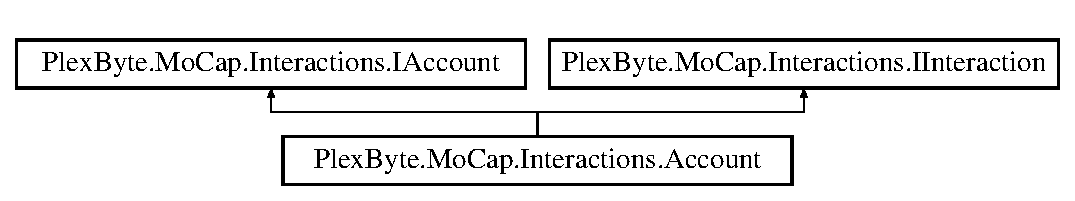
\includegraphics[height=2.000000cm]{class_plex_byte_1_1_mo_cap_1_1_interactions_1_1_account}
\end{center}
\end{figure}
\subsection*{Public Member Functions}
\begin{DoxyCompactItemize}
\item 
\hyperlink{class_plex_byte_1_1_mo_cap_1_1_interactions_1_1_account_a067473555d22524f93c988371c7ae0b8}{Account} (string p\+Id, string p\+Text, I\+User p\+Creator)
\begin{DoxyCompactList}\small\item\em Constructor of the class \end{DoxyCompactList}\item 
\hyperlink{class_plex_byte_1_1_mo_cap_1_1_interactions_1_1_account_a2143d30349b9dce3d6e154ac51a34829}{Account} (string p\+Id, string p\+Text, List$<$ \hyperlink{interface_plex_byte_1_1_mo_cap_1_1_interactions_1_1_i_expense}{I\+Expense} $>$ p\+Expense\+List, List$<$ \hyperlink{interface_plex_byte_1_1_mo_cap_1_1_interactions_1_1_i_timeslice}{I\+Timeslice} $>$ p\+Timeslice\+List, I\+User p\+Creator)
\begin{DoxyCompactList}\small\item\em Constructor of the class \end{DoxyCompactList}\item 
virtual void \hyperlink{class_plex_byte_1_1_mo_cap_1_1_interactions_1_1_account_a697e062e9b46c58922cbdce34b8e1574}{On\+Complete} (\hyperlink{class_plex_byte_1_1_mo_cap_1_1_interactions_1_1_interaction_event_args}{Interaction\+Event\+Args} p\+Event\+Args)
\begin{DoxyCompactList}\small\item\em This method raises the corresponding event in case subscribers are registered \end{DoxyCompactList}\item 
virtual void \hyperlink{class_plex_byte_1_1_mo_cap_1_1_interactions_1_1_account_a8b3878783c7aa0648adc8633e98e7f4e}{On\+Modify} (\hyperlink{class_plex_byte_1_1_mo_cap_1_1_interactions_1_1_interaction_event_args}{Interaction\+Event\+Args} p\+Event\+Args)
\begin{DoxyCompactList}\small\item\em This method raises the corresponding event in case subscribers are registered \end{DoxyCompactList}\item 
virtual void \hyperlink{class_plex_byte_1_1_mo_cap_1_1_interactions_1_1_account_aea5d67faea2dcce6ed0deff84274e9ad}{On\+State\+Changed} (\hyperlink{class_plex_byte_1_1_mo_cap_1_1_interactions_1_1_interaction_event_args}{Interaction\+Event\+Args} p\+Event\+Args)
\begin{DoxyCompactList}\small\item\em This method raises the corresponding event in case subscribers are registered \end{DoxyCompactList}\item 
virtual void \hyperlink{class_plex_byte_1_1_mo_cap_1_1_interactions_1_1_account_a85ea096cc8598da7ec635311e20c77f4}{On\+Expense\+Added} (\hyperlink{class_plex_byte_1_1_mo_cap_1_1_interactions_1_1_interaction_event_args}{Interaction\+Event\+Args} p\+Event\+Args)
\begin{DoxyCompactList}\small\item\em This method raises the corresponding event in case subscribers are registered \end{DoxyCompactList}\item 
virtual void \hyperlink{class_plex_byte_1_1_mo_cap_1_1_interactions_1_1_account_a978de8f575c4f196808d37836c960202}{On\+Timeslice\+Added} (\hyperlink{class_plex_byte_1_1_mo_cap_1_1_interactions_1_1_interaction_event_args}{Interaction\+Event\+Args} p\+Event\+Args)
\begin{DoxyCompactList}\small\item\em This method raises the corresponding event in case subscribers are registered \end{DoxyCompactList}\item 
virtual void \hyperlink{class_plex_byte_1_1_mo_cap_1_1_interactions_1_1_account_a7220958b8470021790726ae8e68078a5}{Change\+Owner} (I\+User p\+User)
\begin{DoxyCompactList}\small\item\em This method changes the owner of the project and raises the modified event if the owner is different used to create a secound project-\/admin \end{DoxyCompactList}\item 
virtual void \hyperlink{class_plex_byte_1_1_mo_cap_1_1_interactions_1_1_account_aa599051753ac017c4fa2613fa16be415}{Change\+Is\+Active} (bool p\+Active)
\begin{DoxyCompactList}\small\item\em This method changes the active flag of the object. This can occure if the item expired, finished or was cancelled. It will raise the Modified event once changed \end{DoxyCompactList}\item 
virtual void \hyperlink{class_plex_byte_1_1_mo_cap_1_1_interactions_1_1_account_a3dadb5bcabffdec7afad04af7c94e2f0}{Change\+State} (\hyperlink{namespace_plex_byte_1_1_mo_cap_1_1_interactions_afcb673d9186608b6bd3b187179aedc8a}{Interaction\+State} p\+State)
\begin{DoxyCompactList}\small\item\em Changes the state of this interaction and thus causes the state\+C\+Hanged event to be fired \end{DoxyCompactList}\item 
void \hyperlink{class_plex_byte_1_1_mo_cap_1_1_interactions_1_1_account_a0f69931bd1d21cb3692f0f08918247bd}{Add\+Expense} (\hyperlink{interface_plex_byte_1_1_mo_cap_1_1_interactions_1_1_i_expense}{I\+Expense} p\+Expense)
\begin{DoxyCompactList}\small\item\em Adds a \char`\"{}expense\char`\"{} to the expenselist \end{DoxyCompactList}\item 
void \hyperlink{class_plex_byte_1_1_mo_cap_1_1_interactions_1_1_account_a28d01e56bb3fc78f30f4ed5f259c0e17}{Add\+Timeslice} (\hyperlink{interface_plex_byte_1_1_mo_cap_1_1_interactions_1_1_i_timeslice}{I\+Timeslice} p\+Timeslice)
\begin{DoxyCompactList}\small\item\em Adds a \char`\"{}timeslice\char`\"{} to the timeslicelist \end{DoxyCompactList}\item 
void \hyperlink{class_plex_byte_1_1_mo_cap_1_1_interactions_1_1_account_a84d71e01b4a2a2483b52bc67635499ed}{Delete\+Expense} (\hyperlink{interface_plex_byte_1_1_mo_cap_1_1_interactions_1_1_i_expense}{I\+Expense} p\+Expense)
\begin{DoxyCompactList}\small\item\em Deletes a \char`\"{}expense\char`\"{} object if it exists in the expenselist \end{DoxyCompactList}\item 
void \hyperlink{class_plex_byte_1_1_mo_cap_1_1_interactions_1_1_account_a3baea063609ff894849c852c249a3c7a}{Edit\+Timeslice} (\hyperlink{interface_plex_byte_1_1_mo_cap_1_1_interactions_1_1_i_timeslice}{I\+Timeslice} p\+Timeslice, \hyperlink{interface_plex_byte_1_1_mo_cap_1_1_interactions_1_1_i_timeslice}{I\+Timeslice} p\+New\+Timeslice)
\begin{DoxyCompactList}\small\item\em To edit the timeslice the old one is removed and a new is being created \end{DoxyCompactList}\item 
void \hyperlink{class_plex_byte_1_1_mo_cap_1_1_interactions_1_1_account_a8b8d09b65d60431bdbbef7d3aed6a72b}{Delete\+Timeslice} (\hyperlink{interface_plex_byte_1_1_mo_cap_1_1_interactions_1_1_i_timeslice}{I\+Timeslice} p\+Timeslice)
\begin{DoxyCompactList}\small\item\em Deletes a \char`\"{}timeslice\char`\"{} object if it exists in the timeslicelist \end{DoxyCompactList}\item 
decimal \hyperlink{class_plex_byte_1_1_mo_cap_1_1_interactions_1_1_account_a44cddcf32dbd3ce31fc012104f25e9f8}{User\+Expense} (I\+User p\+User)
\begin{DoxyCompactList}\small\item\em Returns the overall expenses of an User in the project \end{DoxyCompactList}\item 
int \hyperlink{class_plex_byte_1_1_mo_cap_1_1_interactions_1_1_account_a77706a7728657fb56f5f5dc85bd738f4}{User\+Timeslice} (I\+User p\+User)
\begin{DoxyCompactList}\small\item\em Returns the overall time of an User in the project \end{DoxyCompactList}\end{DoxyCompactItemize}
\subsection*{Properties}
\begin{DoxyCompactItemize}
\item 
string \hyperlink{class_plex_byte_1_1_mo_cap_1_1_interactions_1_1_account_a803b3019d6baa78793eeb56e9033028a}{Id}\hspace{0.3cm}{\ttfamily  \mbox{[}get\mbox{]}}
\begin{DoxyCompactList}\small\item\em The unique id of the account \end{DoxyCompactList}\item 
Date\+Time \hyperlink{class_plex_byte_1_1_mo_cap_1_1_interactions_1_1_account_a5e26981bffb5bdee06beb50888553ec0}{Start\+Date\+Time}\hspace{0.3cm}{\ttfamily  \mbox{[}get, set\mbox{]}}
\begin{DoxyCompactList}\small\item\em The date and time this account becomes active and can be worked on. As long as this date is not reached the state will remain queued and no work can be performed on the account as longs as it is in state queued \end{DoxyCompactList}\item 
Date\+Time \hyperlink{class_plex_byte_1_1_mo_cap_1_1_interactions_1_1_account_a15dfe505b42a142c4a4fc0ec93ab7fba}{End\+Date\+Time}\hspace{0.3cm}{\ttfamily  \mbox{[}get, set\mbox{]}}
\begin{DoxyCompactList}\small\item\em The date and time this account should be finished. If this date is reached the state will change to expired \end{DoxyCompactList}\item 
Date\+Time \hyperlink{class_plex_byte_1_1_mo_cap_1_1_interactions_1_1_account_a5479e6c738ee5788378895820d71e24a}{Created\+Date\+Time}\hspace{0.3cm}{\ttfamily  \mbox{[}get\mbox{]}}
\begin{DoxyCompactList}\small\item\em The date and time the account was created \end{DoxyCompactList}\item 
Date\+Time \hyperlink{class_plex_byte_1_1_mo_cap_1_1_interactions_1_1_account_af8af891d5ca86bc5aec5403339aefa76}{Modified\+Date\+Time}\hspace{0.3cm}{\ttfamily  \mbox{[}get, set\mbox{]}}
\begin{DoxyCompactList}\small\item\em The date and time the account was last modified \end{DoxyCompactList}\item 
bool \hyperlink{class_plex_byte_1_1_mo_cap_1_1_interactions_1_1_account_adce5e94f1e2ca7340805ad6f601ebe5f}{Is\+Active}\hspace{0.3cm}{\ttfamily  \mbox{[}get\mbox{]}}
\begin{DoxyCompactList}\small\item\em Flag indicating whether or not the account can be worked on \end{DoxyCompactList}\item 
string \hyperlink{class_plex_byte_1_1_mo_cap_1_1_interactions_1_1_account_a271c6c603f997216f42f290de1dc89eb}{Text}\hspace{0.3cm}{\ttfamily  \mbox{[}get, set\mbox{]}}
\begin{DoxyCompactList}\small\item\em The text of this account (description) \end{DoxyCompactList}\item 
\hyperlink{namespace_plex_byte_1_1_mo_cap_1_1_interactions_a6e7bea333446664bbce2bb296db25e31}{Interaction\+Type} \hyperlink{class_plex_byte_1_1_mo_cap_1_1_interactions_1_1_account_ab8c590e09224e5015e66019cec50280c}{Type}\hspace{0.3cm}{\ttfamily  \mbox{[}get\mbox{]}}
\begin{DoxyCompactList}\small\item\em The type of interaction (will be always account) \end{DoxyCompactList}\item 
I\+User \hyperlink{class_plex_byte_1_1_mo_cap_1_1_interactions_1_1_account_ab04766b742ba744b403e1e24f702b0d1}{Creator}\hspace{0.3cm}{\ttfamily  \mbox{[}get\mbox{]}}
\begin{DoxyCompactList}\small\item\em The user that created the account \end{DoxyCompactList}\item 
I\+User \hyperlink{class_plex_byte_1_1_mo_cap_1_1_interactions_1_1_account_a36d8ba4726f5289eabc6173ad9e910d6}{Owner}\hspace{0.3cm}{\ttfamily  \mbox{[}get, set\mbox{]}}
\begin{DoxyCompactList}\small\item\em The user currently owning the account \end{DoxyCompactList}\item 
\hyperlink{namespace_plex_byte_1_1_mo_cap_1_1_interactions_afcb673d9186608b6bd3b187179aedc8a}{Interaction\+State} \hyperlink{class_plex_byte_1_1_mo_cap_1_1_interactions_1_1_account_aed386d136f63df4fedd54b91c609512e}{State}\hspace{0.3cm}{\ttfamily  \mbox{[}get\mbox{]}}
\begin{DoxyCompactList}\small\item\em The state of the account \end{DoxyCompactList}\item 
List$<$ \hyperlink{interface_plex_byte_1_1_mo_cap_1_1_interactions_1_1_i_expense}{I\+Expense} $>$ \hyperlink{class_plex_byte_1_1_mo_cap_1_1_interactions_1_1_account_a01eaa284f3668b214462e51ef13b7fd8}{Expense\+List}\hspace{0.3cm}{\ttfamily  \mbox{[}get\mbox{]}}
\begin{DoxyCompactList}\small\item\em A list of all expense-\/objects \end{DoxyCompactList}\item 
List$<$ \hyperlink{interface_plex_byte_1_1_mo_cap_1_1_interactions_1_1_i_timeslice}{I\+Timeslice} $>$ \hyperlink{class_plex_byte_1_1_mo_cap_1_1_interactions_1_1_account_a0a45c7a5a420fde27cfc1c008a7023f1}{Timeslice\+List}\hspace{0.3cm}{\ttfamily  \mbox{[}get\mbox{]}}
\begin{DoxyCompactList}\small\item\em A list of all timeslice-\/objects \end{DoxyCompactList}\end{DoxyCompactItemize}
\subsection*{Events}
\begin{DoxyCompactItemize}
\item 
\hyperlink{namespace_plex_byte_1_1_mo_cap_1_1_interactions_ac81ac3321ab2b018c75ad2c18ec15b9e}{Complete} \hyperlink{class_plex_byte_1_1_mo_cap_1_1_interactions_1_1_account_a2d975974095e091d66e21cfa2d28b9ab}{Completed}
\item 
\hyperlink{namespace_plex_byte_1_1_mo_cap_1_1_interactions_a490186f613e46adce26244f3b2c78a58}{Modify} \hyperlink{class_plex_byte_1_1_mo_cap_1_1_interactions_1_1_account_a79a653b390e022a26200899b77c276cf}{Modified}
\item 
\hyperlink{namespace_plex_byte_1_1_mo_cap_1_1_interactions_af2ff213e81451f96fc74bfad114cecde}{State\+Change} \hyperlink{class_plex_byte_1_1_mo_cap_1_1_interactions_1_1_account_a0a0a49e58be6492cce544f8a6009dc52}{State\+Changed}
\item 
\hyperlink{namespace_plex_byte_1_1_mo_cap_1_1_interactions_a7c03c08c6f524b34193985c455985f1f}{Expense\+Add} \hyperlink{class_plex_byte_1_1_mo_cap_1_1_interactions_1_1_account_ad96bd65da3c69c282a266761593c7cd7}{Expense\+Added}
\item 
\hyperlink{namespace_plex_byte_1_1_mo_cap_1_1_interactions_a600557b92ababd90f6a91c524998565a}{Timeslice\+Add} \hyperlink{class_plex_byte_1_1_mo_cap_1_1_interactions_1_1_account_a10f5bed89fdad33cafcb018e3f4f7bd8}{Timeslice\+Added}
\end{DoxyCompactItemize}


\subsection{Detailed Description}


Definition at line 11 of file Account.\+cs.



\subsection{Constructor \& Destructor Documentation}
\index{Plex\+Byte\+::\+Mo\+Cap\+::\+Interactions\+::\+Account@{Plex\+Byte\+::\+Mo\+Cap\+::\+Interactions\+::\+Account}!Account@{Account}}
\index{Account@{Account}!Plex\+Byte\+::\+Mo\+Cap\+::\+Interactions\+::\+Account@{Plex\+Byte\+::\+Mo\+Cap\+::\+Interactions\+::\+Account}}
\subsubsection[{\texorpdfstring{Account(string p\+Id, string p\+Text, I\+User p\+Creator)}{Account(string pId, string pText, IUser pCreator)}}]{\setlength{\rightskip}{0pt plus 5cm}Plex\+Byte.\+Mo\+Cap.\+Interactions.\+Account.\+Account (
\begin{DoxyParamCaption}
\item[{string}]{p\+Id, }
\item[{string}]{p\+Text, }
\item[{I\+User}]{p\+Creator}
\end{DoxyParamCaption}
)}\hypertarget{class_plex_byte_1_1_mo_cap_1_1_interactions_1_1_account_a067473555d22524f93c988371c7ae0b8}{}\label{class_plex_byte_1_1_mo_cap_1_1_interactions_1_1_account_a067473555d22524f93c988371c7ae0b8}


Constructor of the class 


\begin{DoxyParams}{Parameters}
{\em p\+Id} & \\
\hline
{\em p\+Text} & \\
\hline
{\em p\+Creator} & \\
\hline
\end{DoxyParams}


Definition at line 95 of file Account.\+cs.

\index{Plex\+Byte\+::\+Mo\+Cap\+::\+Interactions\+::\+Account@{Plex\+Byte\+::\+Mo\+Cap\+::\+Interactions\+::\+Account}!Account@{Account}}
\index{Account@{Account}!Plex\+Byte\+::\+Mo\+Cap\+::\+Interactions\+::\+Account@{Plex\+Byte\+::\+Mo\+Cap\+::\+Interactions\+::\+Account}}
\subsubsection[{\texorpdfstring{Account(string p\+Id, string p\+Text, List$<$ I\+Expense $>$ p\+Expense\+List, List$<$ I\+Timeslice $>$ p\+Timeslice\+List, I\+User p\+Creator)}{Account(string pId, string pText, List< IExpense > pExpenseList, List< ITimeslice > pTimesliceList, IUser pCreator)}}]{\setlength{\rightskip}{0pt plus 5cm}Plex\+Byte.\+Mo\+Cap.\+Interactions.\+Account.\+Account (
\begin{DoxyParamCaption}
\item[{string}]{p\+Id, }
\item[{string}]{p\+Text, }
\item[{List$<$ {\bf I\+Expense} $>$}]{p\+Expense\+List, }
\item[{List$<$ {\bf I\+Timeslice} $>$}]{p\+Timeslice\+List, }
\item[{I\+User}]{p\+Creator}
\end{DoxyParamCaption}
)}\hypertarget{class_plex_byte_1_1_mo_cap_1_1_interactions_1_1_account_a2143d30349b9dce3d6e154ac51a34829}{}\label{class_plex_byte_1_1_mo_cap_1_1_interactions_1_1_account_a2143d30349b9dce3d6e154ac51a34829}


Constructor of the class 


\begin{DoxyParams}{Parameters}
{\em p\+Id} & \\
\hline
{\em p\+Text} & \\
\hline
{\em p\+Enable\+Balance} & \\
\hline
{\em p\+Enable\+Survey} & \\
\hline
{\em p\+Creator} & \\
\hline
{\em p\+Member\+List} & \\
\hline
{\em p\+Invitation\+List} & \\
\hline
\end{DoxyParams}


Definition at line 115 of file Account.\+cs.



\subsection{Member Function Documentation}
\index{Plex\+Byte\+::\+Mo\+Cap\+::\+Interactions\+::\+Account@{Plex\+Byte\+::\+Mo\+Cap\+::\+Interactions\+::\+Account}!Add\+Expense@{Add\+Expense}}
\index{Add\+Expense@{Add\+Expense}!Plex\+Byte\+::\+Mo\+Cap\+::\+Interactions\+::\+Account@{Plex\+Byte\+::\+Mo\+Cap\+::\+Interactions\+::\+Account}}
\subsubsection[{\texorpdfstring{Add\+Expense(\+I\+Expense p\+Expense)}{AddExpense(IExpense pExpense)}}]{\setlength{\rightskip}{0pt plus 5cm}void Plex\+Byte.\+Mo\+Cap.\+Interactions.\+Account.\+Add\+Expense (
\begin{DoxyParamCaption}
\item[{{\bf I\+Expense}}]{p\+Expense}
\end{DoxyParamCaption}
)}\hypertarget{class_plex_byte_1_1_mo_cap_1_1_interactions_1_1_account_a0f69931bd1d21cb3692f0f08918247bd}{}\label{class_plex_byte_1_1_mo_cap_1_1_interactions_1_1_account_a0f69931bd1d21cb3692f0f08918247bd}


Adds a \char`\"{}expense\char`\"{} to the expenselist 


\begin{DoxyParams}{Parameters}
{\em p\+Expense} & \\
\hline
\end{DoxyParams}


Implements \hyperlink{interface_plex_byte_1_1_mo_cap_1_1_interactions_1_1_i_account_a824d1d5e807efd91b8b5297c17615181}{Plex\+Byte.\+Mo\+Cap.\+Interactions.\+I\+Account}.



Definition at line 223 of file Account.\+cs.

\index{Plex\+Byte\+::\+Mo\+Cap\+::\+Interactions\+::\+Account@{Plex\+Byte\+::\+Mo\+Cap\+::\+Interactions\+::\+Account}!Add\+Timeslice@{Add\+Timeslice}}
\index{Add\+Timeslice@{Add\+Timeslice}!Plex\+Byte\+::\+Mo\+Cap\+::\+Interactions\+::\+Account@{Plex\+Byte\+::\+Mo\+Cap\+::\+Interactions\+::\+Account}}
\subsubsection[{\texorpdfstring{Add\+Timeslice(\+I\+Timeslice p\+Timeslice)}{AddTimeslice(ITimeslice pTimeslice)}}]{\setlength{\rightskip}{0pt plus 5cm}void Plex\+Byte.\+Mo\+Cap.\+Interactions.\+Account.\+Add\+Timeslice (
\begin{DoxyParamCaption}
\item[{{\bf I\+Timeslice}}]{p\+Timeslice}
\end{DoxyParamCaption}
)}\hypertarget{class_plex_byte_1_1_mo_cap_1_1_interactions_1_1_account_a28d01e56bb3fc78f30f4ed5f259c0e17}{}\label{class_plex_byte_1_1_mo_cap_1_1_interactions_1_1_account_a28d01e56bb3fc78f30f4ed5f259c0e17}


Adds a \char`\"{}timeslice\char`\"{} to the timeslicelist 


\begin{DoxyParams}{Parameters}
{\em p\+Timeslice} & \\
\hline
\end{DoxyParams}


Implements \hyperlink{interface_plex_byte_1_1_mo_cap_1_1_interactions_1_1_i_account_a32338193fc2a47546efe36dc370b6c1a}{Plex\+Byte.\+Mo\+Cap.\+Interactions.\+I\+Account}.



Definition at line 235 of file Account.\+cs.

\index{Plex\+Byte\+::\+Mo\+Cap\+::\+Interactions\+::\+Account@{Plex\+Byte\+::\+Mo\+Cap\+::\+Interactions\+::\+Account}!Change\+Is\+Active@{Change\+Is\+Active}}
\index{Change\+Is\+Active@{Change\+Is\+Active}!Plex\+Byte\+::\+Mo\+Cap\+::\+Interactions\+::\+Account@{Plex\+Byte\+::\+Mo\+Cap\+::\+Interactions\+::\+Account}}
\subsubsection[{\texorpdfstring{Change\+Is\+Active(bool p\+Active)}{ChangeIsActive(bool pActive)}}]{\setlength{\rightskip}{0pt plus 5cm}virtual void Plex\+Byte.\+Mo\+Cap.\+Interactions.\+Account.\+Change\+Is\+Active (
\begin{DoxyParamCaption}
\item[{bool}]{p\+Active}
\end{DoxyParamCaption}
)\hspace{0.3cm}{\ttfamily [virtual]}}\hypertarget{class_plex_byte_1_1_mo_cap_1_1_interactions_1_1_account_aa599051753ac017c4fa2613fa16be415}{}\label{class_plex_byte_1_1_mo_cap_1_1_interactions_1_1_account_aa599051753ac017c4fa2613fa16be415}


This method changes the active flag of the object. This can occure if the item expired, finished or was cancelled. It will raise the Modified event once changed 


\begin{DoxyParams}{Parameters}
{\em p\+Active} & \\
\hline
\end{DoxyParams}


Implements \hyperlink{interface_plex_byte_1_1_mo_cap_1_1_interactions_1_1_i_interaction_ac2d9f47a1139b931939e8cff07153aba}{Plex\+Byte.\+Mo\+Cap.\+Interactions.\+I\+Interaction}.



Definition at line 193 of file Account.\+cs.

\index{Plex\+Byte\+::\+Mo\+Cap\+::\+Interactions\+::\+Account@{Plex\+Byte\+::\+Mo\+Cap\+::\+Interactions\+::\+Account}!Change\+Owner@{Change\+Owner}}
\index{Change\+Owner@{Change\+Owner}!Plex\+Byte\+::\+Mo\+Cap\+::\+Interactions\+::\+Account@{Plex\+Byte\+::\+Mo\+Cap\+::\+Interactions\+::\+Account}}
\subsubsection[{\texorpdfstring{Change\+Owner(\+I\+User p\+User)}{ChangeOwner(IUser pUser)}}]{\setlength{\rightskip}{0pt plus 5cm}virtual void Plex\+Byte.\+Mo\+Cap.\+Interactions.\+Account.\+Change\+Owner (
\begin{DoxyParamCaption}
\item[{I\+User}]{p\+User}
\end{DoxyParamCaption}
)\hspace{0.3cm}{\ttfamily [virtual]}}\hypertarget{class_plex_byte_1_1_mo_cap_1_1_interactions_1_1_account_a7220958b8470021790726ae8e68078a5}{}\label{class_plex_byte_1_1_mo_cap_1_1_interactions_1_1_account_a7220958b8470021790726ae8e68078a5}


This method changes the owner of the project and raises the modified event if the owner is different used to create a secound project-\/admin 


\begin{DoxyParams}{Parameters}
{\em p\+User} & \\
\hline
\end{DoxyParams}


Implements \hyperlink{interface_plex_byte_1_1_mo_cap_1_1_interactions_1_1_i_interaction_a7e3b0a67dc7d176877b8b94922a9bb52}{Plex\+Byte.\+Mo\+Cap.\+Interactions.\+I\+Interaction}.



Definition at line 177 of file Account.\+cs.

\index{Plex\+Byte\+::\+Mo\+Cap\+::\+Interactions\+::\+Account@{Plex\+Byte\+::\+Mo\+Cap\+::\+Interactions\+::\+Account}!Change\+State@{Change\+State}}
\index{Change\+State@{Change\+State}!Plex\+Byte\+::\+Mo\+Cap\+::\+Interactions\+::\+Account@{Plex\+Byte\+::\+Mo\+Cap\+::\+Interactions\+::\+Account}}
\subsubsection[{\texorpdfstring{Change\+State(\+Interaction\+State p\+State)}{ChangeState(InteractionState pState)}}]{\setlength{\rightskip}{0pt plus 5cm}virtual void Plex\+Byte.\+Mo\+Cap.\+Interactions.\+Account.\+Change\+State (
\begin{DoxyParamCaption}
\item[{{\bf Interaction\+State}}]{p\+State}
\end{DoxyParamCaption}
)\hspace{0.3cm}{\ttfamily [virtual]}}\hypertarget{class_plex_byte_1_1_mo_cap_1_1_interactions_1_1_account_a3dadb5bcabffdec7afad04af7c94e2f0}{}\label{class_plex_byte_1_1_mo_cap_1_1_interactions_1_1_account_a3dadb5bcabffdec7afad04af7c94e2f0}


Changes the state of this interaction and thus causes the state\+C\+Hanged event to be fired 


\begin{DoxyParams}{Parameters}
{\em p\+State} & \\
\hline
\end{DoxyParams}


Implements \hyperlink{interface_plex_byte_1_1_mo_cap_1_1_interactions_1_1_i_interaction_a10beb35eb6061878469b5a6cd5431b32}{Plex\+Byte.\+Mo\+Cap.\+Interactions.\+I\+Interaction}.



Definition at line 208 of file Account.\+cs.

\index{Plex\+Byte\+::\+Mo\+Cap\+::\+Interactions\+::\+Account@{Plex\+Byte\+::\+Mo\+Cap\+::\+Interactions\+::\+Account}!Delete\+Expense@{Delete\+Expense}}
\index{Delete\+Expense@{Delete\+Expense}!Plex\+Byte\+::\+Mo\+Cap\+::\+Interactions\+::\+Account@{Plex\+Byte\+::\+Mo\+Cap\+::\+Interactions\+::\+Account}}
\subsubsection[{\texorpdfstring{Delete\+Expense(\+I\+Expense p\+Expense)}{DeleteExpense(IExpense pExpense)}}]{\setlength{\rightskip}{0pt plus 5cm}void Plex\+Byte.\+Mo\+Cap.\+Interactions.\+Account.\+Delete\+Expense (
\begin{DoxyParamCaption}
\item[{{\bf I\+Expense}}]{p\+Expense}
\end{DoxyParamCaption}
)}\hypertarget{class_plex_byte_1_1_mo_cap_1_1_interactions_1_1_account_a84d71e01b4a2a2483b52bc67635499ed}{}\label{class_plex_byte_1_1_mo_cap_1_1_interactions_1_1_account_a84d71e01b4a2a2483b52bc67635499ed}


Deletes a \char`\"{}expense\char`\"{} object if it exists in the expenselist 


\begin{DoxyParams}{Parameters}
{\em p\+Expense} & \\
\hline
\end{DoxyParams}


Implements \hyperlink{interface_plex_byte_1_1_mo_cap_1_1_interactions_1_1_i_account_aa16e3839c2d7eeb4b18dd883ba913533}{Plex\+Byte.\+Mo\+Cap.\+Interactions.\+I\+Account}.



Definition at line 247 of file Account.\+cs.

\index{Plex\+Byte\+::\+Mo\+Cap\+::\+Interactions\+::\+Account@{Plex\+Byte\+::\+Mo\+Cap\+::\+Interactions\+::\+Account}!Delete\+Timeslice@{Delete\+Timeslice}}
\index{Delete\+Timeslice@{Delete\+Timeslice}!Plex\+Byte\+::\+Mo\+Cap\+::\+Interactions\+::\+Account@{Plex\+Byte\+::\+Mo\+Cap\+::\+Interactions\+::\+Account}}
\subsubsection[{\texorpdfstring{Delete\+Timeslice(\+I\+Timeslice p\+Timeslice)}{DeleteTimeslice(ITimeslice pTimeslice)}}]{\setlength{\rightskip}{0pt plus 5cm}void Plex\+Byte.\+Mo\+Cap.\+Interactions.\+Account.\+Delete\+Timeslice (
\begin{DoxyParamCaption}
\item[{{\bf I\+Timeslice}}]{p\+Timeslice}
\end{DoxyParamCaption}
)}\hypertarget{class_plex_byte_1_1_mo_cap_1_1_interactions_1_1_account_a8b8d09b65d60431bdbbef7d3aed6a72b}{}\label{class_plex_byte_1_1_mo_cap_1_1_interactions_1_1_account_a8b8d09b65d60431bdbbef7d3aed6a72b}


Deletes a \char`\"{}timeslice\char`\"{} object if it exists in the timeslicelist 


\begin{DoxyParams}{Parameters}
{\em p\+Timeslice} & \\
\hline
\end{DoxyParams}


Implements \hyperlink{interface_plex_byte_1_1_mo_cap_1_1_interactions_1_1_i_account_a28f21a9fd3584256cc0f5eeb41477e06}{Plex\+Byte.\+Mo\+Cap.\+Interactions.\+I\+Account}.



Definition at line 278 of file Account.\+cs.

\index{Plex\+Byte\+::\+Mo\+Cap\+::\+Interactions\+::\+Account@{Plex\+Byte\+::\+Mo\+Cap\+::\+Interactions\+::\+Account}!Edit\+Timeslice@{Edit\+Timeslice}}
\index{Edit\+Timeslice@{Edit\+Timeslice}!Plex\+Byte\+::\+Mo\+Cap\+::\+Interactions\+::\+Account@{Plex\+Byte\+::\+Mo\+Cap\+::\+Interactions\+::\+Account}}
\subsubsection[{\texorpdfstring{Edit\+Timeslice(\+I\+Timeslice p\+Timeslice, I\+Timeslice p\+New\+Timeslice)}{EditTimeslice(ITimeslice pTimeslice, ITimeslice pNewTimeslice)}}]{\setlength{\rightskip}{0pt plus 5cm}void Plex\+Byte.\+Mo\+Cap.\+Interactions.\+Account.\+Edit\+Timeslice (
\begin{DoxyParamCaption}
\item[{{\bf I\+Timeslice}}]{p\+Timeslice, }
\item[{{\bf I\+Timeslice}}]{p\+New\+Timeslice}
\end{DoxyParamCaption}
)}\hypertarget{class_plex_byte_1_1_mo_cap_1_1_interactions_1_1_account_a3baea063609ff894849c852c249a3c7a}{}\label{class_plex_byte_1_1_mo_cap_1_1_interactions_1_1_account_a3baea063609ff894849c852c249a3c7a}


To edit the timeslice the old one is removed and a new is being created 


\begin{DoxyParams}{Parameters}
{\em P\+Timeslice} & \\
\hline
\end{DoxyParams}


Implements \hyperlink{interface_plex_byte_1_1_mo_cap_1_1_interactions_1_1_i_account_ad71ce3f0f04ba8c3563a2e7d1b53378d}{Plex\+Byte.\+Mo\+Cap.\+Interactions.\+I\+Account}.



Definition at line 262 of file Account.\+cs.

\index{Plex\+Byte\+::\+Mo\+Cap\+::\+Interactions\+::\+Account@{Plex\+Byte\+::\+Mo\+Cap\+::\+Interactions\+::\+Account}!On\+Complete@{On\+Complete}}
\index{On\+Complete@{On\+Complete}!Plex\+Byte\+::\+Mo\+Cap\+::\+Interactions\+::\+Account@{Plex\+Byte\+::\+Mo\+Cap\+::\+Interactions\+::\+Account}}
\subsubsection[{\texorpdfstring{On\+Complete(\+Interaction\+Event\+Args p\+Event\+Args)}{OnComplete(InteractionEventArgs pEventArgs)}}]{\setlength{\rightskip}{0pt plus 5cm}virtual void Plex\+Byte.\+Mo\+Cap.\+Interactions.\+Account.\+On\+Complete (
\begin{DoxyParamCaption}
\item[{{\bf Interaction\+Event\+Args}}]{p\+Event\+Args}
\end{DoxyParamCaption}
)\hspace{0.3cm}{\ttfamily [virtual]}}\hypertarget{class_plex_byte_1_1_mo_cap_1_1_interactions_1_1_account_a697e062e9b46c58922cbdce34b8e1574}{}\label{class_plex_byte_1_1_mo_cap_1_1_interactions_1_1_account_a697e062e9b46c58922cbdce34b8e1574}


This method raises the corresponding event in case subscribers are registered 


\begin{DoxyParams}{Parameters}
{\em p\+Event\+Args} & \\
\hline
\end{DoxyParams}


Implements \hyperlink{interface_plex_byte_1_1_mo_cap_1_1_interactions_1_1_i_interaction_a9f32d6c1c2f2ae60dabb274f62128447}{Plex\+Byte.\+Mo\+Cap.\+Interactions.\+I\+Interaction}.



Definition at line 127 of file Account.\+cs.

\index{Plex\+Byte\+::\+Mo\+Cap\+::\+Interactions\+::\+Account@{Plex\+Byte\+::\+Mo\+Cap\+::\+Interactions\+::\+Account}!On\+Expense\+Added@{On\+Expense\+Added}}
\index{On\+Expense\+Added@{On\+Expense\+Added}!Plex\+Byte\+::\+Mo\+Cap\+::\+Interactions\+::\+Account@{Plex\+Byte\+::\+Mo\+Cap\+::\+Interactions\+::\+Account}}
\subsubsection[{\texorpdfstring{On\+Expense\+Added(\+Interaction\+Event\+Args p\+Event\+Args)}{OnExpenseAdded(InteractionEventArgs pEventArgs)}}]{\setlength{\rightskip}{0pt plus 5cm}virtual void Plex\+Byte.\+Mo\+Cap.\+Interactions.\+Account.\+On\+Expense\+Added (
\begin{DoxyParamCaption}
\item[{{\bf Interaction\+Event\+Args}}]{p\+Event\+Args}
\end{DoxyParamCaption}
)\hspace{0.3cm}{\ttfamily [virtual]}}\hypertarget{class_plex_byte_1_1_mo_cap_1_1_interactions_1_1_account_a85ea096cc8598da7ec635311e20c77f4}{}\label{class_plex_byte_1_1_mo_cap_1_1_interactions_1_1_account_a85ea096cc8598da7ec635311e20c77f4}


This method raises the corresponding event in case subscribers are registered 


\begin{DoxyParams}{Parameters}
{\em p\+Event\+Args} & \\
\hline
\end{DoxyParams}


Definition at line 154 of file Account.\+cs.

\index{Plex\+Byte\+::\+Mo\+Cap\+::\+Interactions\+::\+Account@{Plex\+Byte\+::\+Mo\+Cap\+::\+Interactions\+::\+Account}!On\+Modify@{On\+Modify}}
\index{On\+Modify@{On\+Modify}!Plex\+Byte\+::\+Mo\+Cap\+::\+Interactions\+::\+Account@{Plex\+Byte\+::\+Mo\+Cap\+::\+Interactions\+::\+Account}}
\subsubsection[{\texorpdfstring{On\+Modify(\+Interaction\+Event\+Args p\+Event\+Args)}{OnModify(InteractionEventArgs pEventArgs)}}]{\setlength{\rightskip}{0pt plus 5cm}virtual void Plex\+Byte.\+Mo\+Cap.\+Interactions.\+Account.\+On\+Modify (
\begin{DoxyParamCaption}
\item[{{\bf Interaction\+Event\+Args}}]{p\+Event\+Args}
\end{DoxyParamCaption}
)\hspace{0.3cm}{\ttfamily [virtual]}}\hypertarget{class_plex_byte_1_1_mo_cap_1_1_interactions_1_1_account_a8b3878783c7aa0648adc8633e98e7f4e}{}\label{class_plex_byte_1_1_mo_cap_1_1_interactions_1_1_account_a8b3878783c7aa0648adc8633e98e7f4e}


This method raises the corresponding event in case subscribers are registered 


\begin{DoxyParams}{Parameters}
{\em p\+Event\+Args} & \\
\hline
\end{DoxyParams}


Implements \hyperlink{interface_plex_byte_1_1_mo_cap_1_1_interactions_1_1_i_interaction_af4fac42d753ae7f9652541542b8961c6}{Plex\+Byte.\+Mo\+Cap.\+Interactions.\+I\+Interaction}.



Definition at line 136 of file Account.\+cs.

\index{Plex\+Byte\+::\+Mo\+Cap\+::\+Interactions\+::\+Account@{Plex\+Byte\+::\+Mo\+Cap\+::\+Interactions\+::\+Account}!On\+State\+Changed@{On\+State\+Changed}}
\index{On\+State\+Changed@{On\+State\+Changed}!Plex\+Byte\+::\+Mo\+Cap\+::\+Interactions\+::\+Account@{Plex\+Byte\+::\+Mo\+Cap\+::\+Interactions\+::\+Account}}
\subsubsection[{\texorpdfstring{On\+State\+Changed(\+Interaction\+Event\+Args p\+Event\+Args)}{OnStateChanged(InteractionEventArgs pEventArgs)}}]{\setlength{\rightskip}{0pt plus 5cm}virtual void Plex\+Byte.\+Mo\+Cap.\+Interactions.\+Account.\+On\+State\+Changed (
\begin{DoxyParamCaption}
\item[{{\bf Interaction\+Event\+Args}}]{p\+Event\+Args}
\end{DoxyParamCaption}
)\hspace{0.3cm}{\ttfamily [virtual]}}\hypertarget{class_plex_byte_1_1_mo_cap_1_1_interactions_1_1_account_aea5d67faea2dcce6ed0deff84274e9ad}{}\label{class_plex_byte_1_1_mo_cap_1_1_interactions_1_1_account_aea5d67faea2dcce6ed0deff84274e9ad}


This method raises the corresponding event in case subscribers are registered 


\begin{DoxyParams}{Parameters}
{\em p\+Event\+Args} & \\
\hline
\end{DoxyParams}


Implements \hyperlink{interface_plex_byte_1_1_mo_cap_1_1_interactions_1_1_i_interaction_a5250247fb5f22a633e22d7f8dc946c4d}{Plex\+Byte.\+Mo\+Cap.\+Interactions.\+I\+Interaction}.



Definition at line 145 of file Account.\+cs.

\index{Plex\+Byte\+::\+Mo\+Cap\+::\+Interactions\+::\+Account@{Plex\+Byte\+::\+Mo\+Cap\+::\+Interactions\+::\+Account}!On\+Timeslice\+Added@{On\+Timeslice\+Added}}
\index{On\+Timeslice\+Added@{On\+Timeslice\+Added}!Plex\+Byte\+::\+Mo\+Cap\+::\+Interactions\+::\+Account@{Plex\+Byte\+::\+Mo\+Cap\+::\+Interactions\+::\+Account}}
\subsubsection[{\texorpdfstring{On\+Timeslice\+Added(\+Interaction\+Event\+Args p\+Event\+Args)}{OnTimesliceAdded(InteractionEventArgs pEventArgs)}}]{\setlength{\rightskip}{0pt plus 5cm}virtual void Plex\+Byte.\+Mo\+Cap.\+Interactions.\+Account.\+On\+Timeslice\+Added (
\begin{DoxyParamCaption}
\item[{{\bf Interaction\+Event\+Args}}]{p\+Event\+Args}
\end{DoxyParamCaption}
)\hspace{0.3cm}{\ttfamily [virtual]}}\hypertarget{class_plex_byte_1_1_mo_cap_1_1_interactions_1_1_account_a978de8f575c4f196808d37836c960202}{}\label{class_plex_byte_1_1_mo_cap_1_1_interactions_1_1_account_a978de8f575c4f196808d37836c960202}


This method raises the corresponding event in case subscribers are registered 


\begin{DoxyParams}{Parameters}
{\em p\+Event\+Args} & \\
\hline
\end{DoxyParams}


Definition at line 163 of file Account.\+cs.

\index{Plex\+Byte\+::\+Mo\+Cap\+::\+Interactions\+::\+Account@{Plex\+Byte\+::\+Mo\+Cap\+::\+Interactions\+::\+Account}!User\+Expense@{User\+Expense}}
\index{User\+Expense@{User\+Expense}!Plex\+Byte\+::\+Mo\+Cap\+::\+Interactions\+::\+Account@{Plex\+Byte\+::\+Mo\+Cap\+::\+Interactions\+::\+Account}}
\subsubsection[{\texorpdfstring{User\+Expense(\+I\+User p\+User)}{UserExpense(IUser pUser)}}]{\setlength{\rightskip}{0pt plus 5cm}decimal Plex\+Byte.\+Mo\+Cap.\+Interactions.\+Account.\+User\+Expense (
\begin{DoxyParamCaption}
\item[{I\+User}]{p\+User}
\end{DoxyParamCaption}
)}\hypertarget{class_plex_byte_1_1_mo_cap_1_1_interactions_1_1_account_a44cddcf32dbd3ce31fc012104f25e9f8}{}\label{class_plex_byte_1_1_mo_cap_1_1_interactions_1_1_account_a44cddcf32dbd3ce31fc012104f25e9f8}


Returns the overall expenses of an User in the project 


\begin{DoxyParams}{Parameters}
{\em p\+User} & \\
\hline
\end{DoxyParams}
\begin{DoxyReturn}{Returns}
decimal \+\_\+user\+Value
\end{DoxyReturn}


Implements \hyperlink{interface_plex_byte_1_1_mo_cap_1_1_interactions_1_1_i_account_a4a1424e01898012e5457d777006b2a49}{Plex\+Byte.\+Mo\+Cap.\+Interactions.\+I\+Account}.



Definition at line 294 of file Account.\+cs.

\index{Plex\+Byte\+::\+Mo\+Cap\+::\+Interactions\+::\+Account@{Plex\+Byte\+::\+Mo\+Cap\+::\+Interactions\+::\+Account}!User\+Timeslice@{User\+Timeslice}}
\index{User\+Timeslice@{User\+Timeslice}!Plex\+Byte\+::\+Mo\+Cap\+::\+Interactions\+::\+Account@{Plex\+Byte\+::\+Mo\+Cap\+::\+Interactions\+::\+Account}}
\subsubsection[{\texorpdfstring{User\+Timeslice(\+I\+User p\+User)}{UserTimeslice(IUser pUser)}}]{\setlength{\rightskip}{0pt plus 5cm}int Plex\+Byte.\+Mo\+Cap.\+Interactions.\+Account.\+User\+Timeslice (
\begin{DoxyParamCaption}
\item[{I\+User}]{p\+User}
\end{DoxyParamCaption}
)}\hypertarget{class_plex_byte_1_1_mo_cap_1_1_interactions_1_1_account_a77706a7728657fb56f5f5dc85bd738f4}{}\label{class_plex_byte_1_1_mo_cap_1_1_interactions_1_1_account_a77706a7728657fb56f5f5dc85bd738f4}


Returns the overall time of an User in the project 


\begin{DoxyParams}{Parameters}
{\em p\+User} & \\
\hline
\end{DoxyParams}
\begin{DoxyReturn}{Returns}
int \+\_\+user\+Time
\end{DoxyReturn}


Implements \hyperlink{interface_plex_byte_1_1_mo_cap_1_1_interactions_1_1_i_account_a75c8a9171f868234d85ced97117b1b8b}{Plex\+Byte.\+Mo\+Cap.\+Interactions.\+I\+Account}.



Definition at line 311 of file Account.\+cs.



\subsection{Property Documentation}
\index{Plex\+Byte\+::\+Mo\+Cap\+::\+Interactions\+::\+Account@{Plex\+Byte\+::\+Mo\+Cap\+::\+Interactions\+::\+Account}!Created\+Date\+Time@{Created\+Date\+Time}}
\index{Created\+Date\+Time@{Created\+Date\+Time}!Plex\+Byte\+::\+Mo\+Cap\+::\+Interactions\+::\+Account@{Plex\+Byte\+::\+Mo\+Cap\+::\+Interactions\+::\+Account}}
\subsubsection[{\texorpdfstring{Created\+Date\+Time}{CreatedDateTime}}]{\setlength{\rightskip}{0pt plus 5cm}Date\+Time Plex\+Byte.\+Mo\+Cap.\+Interactions.\+Account.\+Created\+Date\+Time\hspace{0.3cm}{\ttfamily [get]}}\hypertarget{class_plex_byte_1_1_mo_cap_1_1_interactions_1_1_account_a5479e6c738ee5788378895820d71e24a}{}\label{class_plex_byte_1_1_mo_cap_1_1_interactions_1_1_account_a5479e6c738ee5788378895820d71e24a}


The date and time the account was created 



Definition at line 31 of file Account.\+cs.

\index{Plex\+Byte\+::\+Mo\+Cap\+::\+Interactions\+::\+Account@{Plex\+Byte\+::\+Mo\+Cap\+::\+Interactions\+::\+Account}!Creator@{Creator}}
\index{Creator@{Creator}!Plex\+Byte\+::\+Mo\+Cap\+::\+Interactions\+::\+Account@{Plex\+Byte\+::\+Mo\+Cap\+::\+Interactions\+::\+Account}}
\subsubsection[{\texorpdfstring{Creator}{Creator}}]{\setlength{\rightskip}{0pt plus 5cm}I\+User Plex\+Byte.\+Mo\+Cap.\+Interactions.\+Account.\+Creator\hspace{0.3cm}{\ttfamily [get]}}\hypertarget{class_plex_byte_1_1_mo_cap_1_1_interactions_1_1_account_ab04766b742ba744b403e1e24f702b0d1}{}\label{class_plex_byte_1_1_mo_cap_1_1_interactions_1_1_account_ab04766b742ba744b403e1e24f702b0d1}


The user that created the account 



Definition at line 51 of file Account.\+cs.

\index{Plex\+Byte\+::\+Mo\+Cap\+::\+Interactions\+::\+Account@{Plex\+Byte\+::\+Mo\+Cap\+::\+Interactions\+::\+Account}!End\+Date\+Time@{End\+Date\+Time}}
\index{End\+Date\+Time@{End\+Date\+Time}!Plex\+Byte\+::\+Mo\+Cap\+::\+Interactions\+::\+Account@{Plex\+Byte\+::\+Mo\+Cap\+::\+Interactions\+::\+Account}}
\subsubsection[{\texorpdfstring{End\+Date\+Time}{EndDateTime}}]{\setlength{\rightskip}{0pt plus 5cm}Date\+Time Plex\+Byte.\+Mo\+Cap.\+Interactions.\+Account.\+End\+Date\+Time\hspace{0.3cm}{\ttfamily [get]}, {\ttfamily [set]}}\hypertarget{class_plex_byte_1_1_mo_cap_1_1_interactions_1_1_account_a15dfe505b42a142c4a4fc0ec93ab7fba}{}\label{class_plex_byte_1_1_mo_cap_1_1_interactions_1_1_account_a15dfe505b42a142c4a4fc0ec93ab7fba}


The date and time this account should be finished. If this date is reached the state will change to expired 



Definition at line 27 of file Account.\+cs.

\index{Plex\+Byte\+::\+Mo\+Cap\+::\+Interactions\+::\+Account@{Plex\+Byte\+::\+Mo\+Cap\+::\+Interactions\+::\+Account}!Expense\+List@{Expense\+List}}
\index{Expense\+List@{Expense\+List}!Plex\+Byte\+::\+Mo\+Cap\+::\+Interactions\+::\+Account@{Plex\+Byte\+::\+Mo\+Cap\+::\+Interactions\+::\+Account}}
\subsubsection[{\texorpdfstring{Expense\+List}{ExpenseList}}]{\setlength{\rightskip}{0pt plus 5cm}List$<${\bf I\+Expense}$>$ Plex\+Byte.\+Mo\+Cap.\+Interactions.\+Account.\+Expense\+List\hspace{0.3cm}{\ttfamily [get]}}\hypertarget{class_plex_byte_1_1_mo_cap_1_1_interactions_1_1_account_a01eaa284f3668b214462e51ef13b7fd8}{}\label{class_plex_byte_1_1_mo_cap_1_1_interactions_1_1_account_a01eaa284f3668b214462e51ef13b7fd8}


A list of all expense-\/objects 



Definition at line 63 of file Account.\+cs.

\index{Plex\+Byte\+::\+Mo\+Cap\+::\+Interactions\+::\+Account@{Plex\+Byte\+::\+Mo\+Cap\+::\+Interactions\+::\+Account}!Id@{Id}}
\index{Id@{Id}!Plex\+Byte\+::\+Mo\+Cap\+::\+Interactions\+::\+Account@{Plex\+Byte\+::\+Mo\+Cap\+::\+Interactions\+::\+Account}}
\subsubsection[{\texorpdfstring{Id}{Id}}]{\setlength{\rightskip}{0pt plus 5cm}string Plex\+Byte.\+Mo\+Cap.\+Interactions.\+Account.\+Id\hspace{0.3cm}{\ttfamily [get]}}\hypertarget{class_plex_byte_1_1_mo_cap_1_1_interactions_1_1_account_a803b3019d6baa78793eeb56e9033028a}{}\label{class_plex_byte_1_1_mo_cap_1_1_interactions_1_1_account_a803b3019d6baa78793eeb56e9033028a}


The unique id of the account 



Definition at line 18 of file Account.\+cs.

\index{Plex\+Byte\+::\+Mo\+Cap\+::\+Interactions\+::\+Account@{Plex\+Byte\+::\+Mo\+Cap\+::\+Interactions\+::\+Account}!Is\+Active@{Is\+Active}}
\index{Is\+Active@{Is\+Active}!Plex\+Byte\+::\+Mo\+Cap\+::\+Interactions\+::\+Account@{Plex\+Byte\+::\+Mo\+Cap\+::\+Interactions\+::\+Account}}
\subsubsection[{\texorpdfstring{Is\+Active}{IsActive}}]{\setlength{\rightskip}{0pt plus 5cm}bool Plex\+Byte.\+Mo\+Cap.\+Interactions.\+Account.\+Is\+Active\hspace{0.3cm}{\ttfamily [get]}}\hypertarget{class_plex_byte_1_1_mo_cap_1_1_interactions_1_1_account_adce5e94f1e2ca7340805ad6f601ebe5f}{}\label{class_plex_byte_1_1_mo_cap_1_1_interactions_1_1_account_adce5e94f1e2ca7340805ad6f601ebe5f}


Flag indicating whether or not the account can be worked on 



Definition at line 39 of file Account.\+cs.

\index{Plex\+Byte\+::\+Mo\+Cap\+::\+Interactions\+::\+Account@{Plex\+Byte\+::\+Mo\+Cap\+::\+Interactions\+::\+Account}!Modified\+Date\+Time@{Modified\+Date\+Time}}
\index{Modified\+Date\+Time@{Modified\+Date\+Time}!Plex\+Byte\+::\+Mo\+Cap\+::\+Interactions\+::\+Account@{Plex\+Byte\+::\+Mo\+Cap\+::\+Interactions\+::\+Account}}
\subsubsection[{\texorpdfstring{Modified\+Date\+Time}{ModifiedDateTime}}]{\setlength{\rightskip}{0pt plus 5cm}Date\+Time Plex\+Byte.\+Mo\+Cap.\+Interactions.\+Account.\+Modified\+Date\+Time\hspace{0.3cm}{\ttfamily [get]}, {\ttfamily [set]}}\hypertarget{class_plex_byte_1_1_mo_cap_1_1_interactions_1_1_account_af8af891d5ca86bc5aec5403339aefa76}{}\label{class_plex_byte_1_1_mo_cap_1_1_interactions_1_1_account_af8af891d5ca86bc5aec5403339aefa76}


The date and time the account was last modified 



Definition at line 35 of file Account.\+cs.

\index{Plex\+Byte\+::\+Mo\+Cap\+::\+Interactions\+::\+Account@{Plex\+Byte\+::\+Mo\+Cap\+::\+Interactions\+::\+Account}!Owner@{Owner}}
\index{Owner@{Owner}!Plex\+Byte\+::\+Mo\+Cap\+::\+Interactions\+::\+Account@{Plex\+Byte\+::\+Mo\+Cap\+::\+Interactions\+::\+Account}}
\subsubsection[{\texorpdfstring{Owner}{Owner}}]{\setlength{\rightskip}{0pt plus 5cm}I\+User Plex\+Byte.\+Mo\+Cap.\+Interactions.\+Account.\+Owner\hspace{0.3cm}{\ttfamily [get]}, {\ttfamily [set]}}\hypertarget{class_plex_byte_1_1_mo_cap_1_1_interactions_1_1_account_a36d8ba4726f5289eabc6173ad9e910d6}{}\label{class_plex_byte_1_1_mo_cap_1_1_interactions_1_1_account_a36d8ba4726f5289eabc6173ad9e910d6}


The user currently owning the account 



Definition at line 55 of file Account.\+cs.

\index{Plex\+Byte\+::\+Mo\+Cap\+::\+Interactions\+::\+Account@{Plex\+Byte\+::\+Mo\+Cap\+::\+Interactions\+::\+Account}!Start\+Date\+Time@{Start\+Date\+Time}}
\index{Start\+Date\+Time@{Start\+Date\+Time}!Plex\+Byte\+::\+Mo\+Cap\+::\+Interactions\+::\+Account@{Plex\+Byte\+::\+Mo\+Cap\+::\+Interactions\+::\+Account}}
\subsubsection[{\texorpdfstring{Start\+Date\+Time}{StartDateTime}}]{\setlength{\rightskip}{0pt plus 5cm}Date\+Time Plex\+Byte.\+Mo\+Cap.\+Interactions.\+Account.\+Start\+Date\+Time\hspace{0.3cm}{\ttfamily [get]}, {\ttfamily [set]}}\hypertarget{class_plex_byte_1_1_mo_cap_1_1_interactions_1_1_account_a5e26981bffb5bdee06beb50888553ec0}{}\label{class_plex_byte_1_1_mo_cap_1_1_interactions_1_1_account_a5e26981bffb5bdee06beb50888553ec0}


The date and time this account becomes active and can be worked on. As long as this date is not reached the state will remain queued and no work can be performed on the account as longs as it is in state queued 



Definition at line 23 of file Account.\+cs.

\index{Plex\+Byte\+::\+Mo\+Cap\+::\+Interactions\+::\+Account@{Plex\+Byte\+::\+Mo\+Cap\+::\+Interactions\+::\+Account}!State@{State}}
\index{State@{State}!Plex\+Byte\+::\+Mo\+Cap\+::\+Interactions\+::\+Account@{Plex\+Byte\+::\+Mo\+Cap\+::\+Interactions\+::\+Account}}
\subsubsection[{\texorpdfstring{State}{State}}]{\setlength{\rightskip}{0pt plus 5cm}{\bf Interaction\+State} Plex\+Byte.\+Mo\+Cap.\+Interactions.\+Account.\+State\hspace{0.3cm}{\ttfamily [get]}}\hypertarget{class_plex_byte_1_1_mo_cap_1_1_interactions_1_1_account_aed386d136f63df4fedd54b91c609512e}{}\label{class_plex_byte_1_1_mo_cap_1_1_interactions_1_1_account_aed386d136f63df4fedd54b91c609512e}


The state of the account 



Definition at line 59 of file Account.\+cs.

\index{Plex\+Byte\+::\+Mo\+Cap\+::\+Interactions\+::\+Account@{Plex\+Byte\+::\+Mo\+Cap\+::\+Interactions\+::\+Account}!Text@{Text}}
\index{Text@{Text}!Plex\+Byte\+::\+Mo\+Cap\+::\+Interactions\+::\+Account@{Plex\+Byte\+::\+Mo\+Cap\+::\+Interactions\+::\+Account}}
\subsubsection[{\texorpdfstring{Text}{Text}}]{\setlength{\rightskip}{0pt plus 5cm}string Plex\+Byte.\+Mo\+Cap.\+Interactions.\+Account.\+Text\hspace{0.3cm}{\ttfamily [get]}, {\ttfamily [set]}}\hypertarget{class_plex_byte_1_1_mo_cap_1_1_interactions_1_1_account_a271c6c603f997216f42f290de1dc89eb}{}\label{class_plex_byte_1_1_mo_cap_1_1_interactions_1_1_account_a271c6c603f997216f42f290de1dc89eb}


The text of this account (description) 



Definition at line 43 of file Account.\+cs.

\index{Plex\+Byte\+::\+Mo\+Cap\+::\+Interactions\+::\+Account@{Plex\+Byte\+::\+Mo\+Cap\+::\+Interactions\+::\+Account}!Timeslice\+List@{Timeslice\+List}}
\index{Timeslice\+List@{Timeslice\+List}!Plex\+Byte\+::\+Mo\+Cap\+::\+Interactions\+::\+Account@{Plex\+Byte\+::\+Mo\+Cap\+::\+Interactions\+::\+Account}}
\subsubsection[{\texorpdfstring{Timeslice\+List}{TimesliceList}}]{\setlength{\rightskip}{0pt plus 5cm}List$<${\bf I\+Timeslice}$>$ Plex\+Byte.\+Mo\+Cap.\+Interactions.\+Account.\+Timeslice\+List\hspace{0.3cm}{\ttfamily [get]}}\hypertarget{class_plex_byte_1_1_mo_cap_1_1_interactions_1_1_account_a0a45c7a5a420fde27cfc1c008a7023f1}{}\label{class_plex_byte_1_1_mo_cap_1_1_interactions_1_1_account_a0a45c7a5a420fde27cfc1c008a7023f1}


A list of all timeslice-\/objects 



Definition at line 67 of file Account.\+cs.

\index{Plex\+Byte\+::\+Mo\+Cap\+::\+Interactions\+::\+Account@{Plex\+Byte\+::\+Mo\+Cap\+::\+Interactions\+::\+Account}!Type@{Type}}
\index{Type@{Type}!Plex\+Byte\+::\+Mo\+Cap\+::\+Interactions\+::\+Account@{Plex\+Byte\+::\+Mo\+Cap\+::\+Interactions\+::\+Account}}
\subsubsection[{\texorpdfstring{Type}{Type}}]{\setlength{\rightskip}{0pt plus 5cm}{\bf Interaction\+Type} Plex\+Byte.\+Mo\+Cap.\+Interactions.\+Account.\+Type\hspace{0.3cm}{\ttfamily [get]}}\hypertarget{class_plex_byte_1_1_mo_cap_1_1_interactions_1_1_account_ab8c590e09224e5015e66019cec50280c}{}\label{class_plex_byte_1_1_mo_cap_1_1_interactions_1_1_account_ab8c590e09224e5015e66019cec50280c}


The type of interaction (will be always account) 



Definition at line 47 of file Account.\+cs.



\subsection{Event Documentation}
\index{Plex\+Byte\+::\+Mo\+Cap\+::\+Interactions\+::\+Account@{Plex\+Byte\+::\+Mo\+Cap\+::\+Interactions\+::\+Account}!Completed@{Completed}}
\index{Completed@{Completed}!Plex\+Byte\+::\+Mo\+Cap\+::\+Interactions\+::\+Account@{Plex\+Byte\+::\+Mo\+Cap\+::\+Interactions\+::\+Account}}
\subsubsection[{\texorpdfstring{Completed}{Completed}}]{\setlength{\rightskip}{0pt plus 5cm}{\bf Complete} Plex\+Byte.\+Mo\+Cap.\+Interactions.\+Account.\+Completed}\hypertarget{class_plex_byte_1_1_mo_cap_1_1_interactions_1_1_account_a2d975974095e091d66e21cfa2d28b9ab}{}\label{class_plex_byte_1_1_mo_cap_1_1_interactions_1_1_account_a2d975974095e091d66e21cfa2d28b9ab}


Definition at line 81 of file Account.\+cs.

\index{Plex\+Byte\+::\+Mo\+Cap\+::\+Interactions\+::\+Account@{Plex\+Byte\+::\+Mo\+Cap\+::\+Interactions\+::\+Account}!Expense\+Added@{Expense\+Added}}
\index{Expense\+Added@{Expense\+Added}!Plex\+Byte\+::\+Mo\+Cap\+::\+Interactions\+::\+Account@{Plex\+Byte\+::\+Mo\+Cap\+::\+Interactions\+::\+Account}}
\subsubsection[{\texorpdfstring{Expense\+Added}{ExpenseAdded}}]{\setlength{\rightskip}{0pt plus 5cm}{\bf Expense\+Add} Plex\+Byte.\+Mo\+Cap.\+Interactions.\+Account.\+Expense\+Added}\hypertarget{class_plex_byte_1_1_mo_cap_1_1_interactions_1_1_account_ad96bd65da3c69c282a266761593c7cd7}{}\label{class_plex_byte_1_1_mo_cap_1_1_interactions_1_1_account_ad96bd65da3c69c282a266761593c7cd7}


Definition at line 84 of file Account.\+cs.

\index{Plex\+Byte\+::\+Mo\+Cap\+::\+Interactions\+::\+Account@{Plex\+Byte\+::\+Mo\+Cap\+::\+Interactions\+::\+Account}!Modified@{Modified}}
\index{Modified@{Modified}!Plex\+Byte\+::\+Mo\+Cap\+::\+Interactions\+::\+Account@{Plex\+Byte\+::\+Mo\+Cap\+::\+Interactions\+::\+Account}}
\subsubsection[{\texorpdfstring{Modified}{Modified}}]{\setlength{\rightskip}{0pt plus 5cm}{\bf Modify} Plex\+Byte.\+Mo\+Cap.\+Interactions.\+Account.\+Modified}\hypertarget{class_plex_byte_1_1_mo_cap_1_1_interactions_1_1_account_a79a653b390e022a26200899b77c276cf}{}\label{class_plex_byte_1_1_mo_cap_1_1_interactions_1_1_account_a79a653b390e022a26200899b77c276cf}


Definition at line 82 of file Account.\+cs.

\index{Plex\+Byte\+::\+Mo\+Cap\+::\+Interactions\+::\+Account@{Plex\+Byte\+::\+Mo\+Cap\+::\+Interactions\+::\+Account}!State\+Changed@{State\+Changed}}
\index{State\+Changed@{State\+Changed}!Plex\+Byte\+::\+Mo\+Cap\+::\+Interactions\+::\+Account@{Plex\+Byte\+::\+Mo\+Cap\+::\+Interactions\+::\+Account}}
\subsubsection[{\texorpdfstring{State\+Changed}{StateChanged}}]{\setlength{\rightskip}{0pt plus 5cm}{\bf State\+Change} Plex\+Byte.\+Mo\+Cap.\+Interactions.\+Account.\+State\+Changed}\hypertarget{class_plex_byte_1_1_mo_cap_1_1_interactions_1_1_account_a0a0a49e58be6492cce544f8a6009dc52}{}\label{class_plex_byte_1_1_mo_cap_1_1_interactions_1_1_account_a0a0a49e58be6492cce544f8a6009dc52}


Definition at line 83 of file Account.\+cs.

\index{Plex\+Byte\+::\+Mo\+Cap\+::\+Interactions\+::\+Account@{Plex\+Byte\+::\+Mo\+Cap\+::\+Interactions\+::\+Account}!Timeslice\+Added@{Timeslice\+Added}}
\index{Timeslice\+Added@{Timeslice\+Added}!Plex\+Byte\+::\+Mo\+Cap\+::\+Interactions\+::\+Account@{Plex\+Byte\+::\+Mo\+Cap\+::\+Interactions\+::\+Account}}
\subsubsection[{\texorpdfstring{Timeslice\+Added}{TimesliceAdded}}]{\setlength{\rightskip}{0pt plus 5cm}{\bf Timeslice\+Add} Plex\+Byte.\+Mo\+Cap.\+Interactions.\+Account.\+Timeslice\+Added}\hypertarget{class_plex_byte_1_1_mo_cap_1_1_interactions_1_1_account_a10f5bed89fdad33cafcb018e3f4f7bd8}{}\label{class_plex_byte_1_1_mo_cap_1_1_interactions_1_1_account_a10f5bed89fdad33cafcb018e3f4f7bd8}


Definition at line 85 of file Account.\+cs.



The documentation for this class was generated from the following file\+:\begin{DoxyCompactItemize}
\item 
D\+:/\+Users/\+Christian\+B/\+Documents/\+\_\+\+H\+F Infomatik/\+Git\+Hub\+\_\+\+Repos/\+Mo\+Cap/\+Plex\+Byte.\+Mo\+Cap/\+Plex\+Byte.\+Mo\+Cap.\+Interactions/\hyperlink{_account_8cs}{Account.\+cs}\end{DoxyCompactItemize}

\hypertarget{class_plex_byte_1_1_mo_cap_1_1_interactions_1_1_expense}{}\section{Plex\+Byte.\+Mo\+Cap.\+Interactions.\+Expense Class Reference}
\label{class_plex_byte_1_1_mo_cap_1_1_interactions_1_1_expense}\index{Plex\+Byte.\+Mo\+Cap.\+Interactions.\+Expense@{Plex\+Byte.\+Mo\+Cap.\+Interactions.\+Expense}}
Inheritance diagram for Plex\+Byte.\+Mo\+Cap.\+Interactions.\+Expense\+:\begin{figure}[H]
\begin{center}
\leavevmode
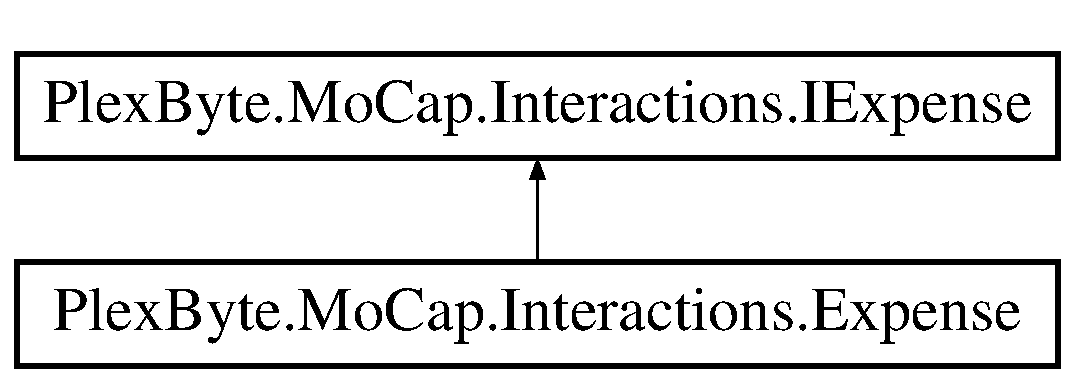
\includegraphics[height=2.000000cm]{class_plex_byte_1_1_mo_cap_1_1_interactions_1_1_expense}
\end{center}
\end{figure}
\subsection*{Public Member Functions}
\begin{DoxyCompactItemize}
\item 
\hyperlink{class_plex_byte_1_1_mo_cap_1_1_interactions_1_1_expense_a2a71f640711b211319c26cf08f86255e}{Expense} (string p\+Id, string p\+Text, I\+User p\+Creator, \hyperlink{interface_plex_byte_1_1_mo_cap_1_1_interactions_1_1_i_interaction}{I\+Interaction} p\+Target)
\begin{DoxyCompactList}\small\item\em Constructor of the class \end{DoxyCompactList}\item 
\hyperlink{class_plex_byte_1_1_mo_cap_1_1_interactions_1_1_expense_a9bb0e412ed6e63676930d4da916e79d6}{Expense} (string p\+Id, string p\+Text, Image p\+Receipt, decimal p\+Value, I\+User p\+Creator, \hyperlink{interface_plex_byte_1_1_mo_cap_1_1_interactions_1_1_i_interaction}{I\+Interaction} p\+Target)
\begin{DoxyCompactList}\small\item\em Constructor of the class \end{DoxyCompactList}\item 
virtual void \hyperlink{class_plex_byte_1_1_mo_cap_1_1_interactions_1_1_expense_a81535f3b98deeaab3e03d190543a4127}{On\+Complete} (\hyperlink{class_plex_byte_1_1_mo_cap_1_1_interactions_1_1_interaction_event_args}{Interaction\+Event\+Args} p\+Event\+Args)
\begin{DoxyCompactList}\small\item\em This method raises the corresponding event in case subscribers are registered \end{DoxyCompactList}\item 
virtual void \hyperlink{class_plex_byte_1_1_mo_cap_1_1_interactions_1_1_expense_a224578edb2ee395588eebd15fcfc29a3}{On\+Modify} (\hyperlink{class_plex_byte_1_1_mo_cap_1_1_interactions_1_1_interaction_event_args}{Interaction\+Event\+Args} p\+Event\+Args)
\begin{DoxyCompactList}\small\item\em This method raises the corresponding event in case subscribers are registered \end{DoxyCompactList}\item 
virtual void \hyperlink{class_plex_byte_1_1_mo_cap_1_1_interactions_1_1_expense_abe824865e6ea9cc7b3d2644e6e0e4069}{On\+State\+Changed} (\hyperlink{class_plex_byte_1_1_mo_cap_1_1_interactions_1_1_interaction_event_args}{Interaction\+Event\+Args} p\+Event\+Args)
\begin{DoxyCompactList}\small\item\em This method raises the corresponding event in case subscribers are registered \end{DoxyCompactList}\item 
void \hyperlink{class_plex_byte_1_1_mo_cap_1_1_interactions_1_1_expense_a33e21b15e70fa450463a5a5197dcfe38}{Add\+Receipt} (Image p\+Receipt)
\begin{DoxyCompactList}\small\item\em Method to add a Receipt to an expense \end{DoxyCompactList}\item 
void \hyperlink{class_plex_byte_1_1_mo_cap_1_1_interactions_1_1_expense_a927ad9089c43c09790083d554b1139f8}{Delete\+Receipt} ()
\begin{DoxyCompactList}\small\item\em Method to remove a Receipt from an expense \end{DoxyCompactList}\item 
void \hyperlink{class_plex_byte_1_1_mo_cap_1_1_interactions_1_1_expense_ace1f3d1404f02fb78583b1709641c2c1}{Edit\+Value} (decimal p\+New\+Value)
\begin{DoxyCompactList}\small\item\em Method to edit the value of an expense \end{DoxyCompactList}\item 
virtual void \hyperlink{class_plex_byte_1_1_mo_cap_1_1_interactions_1_1_expense_a37a7af04bd991bfbfd8619ee3bd35d6c}{Change\+Is\+Active} (bool p\+Active)
\begin{DoxyCompactList}\small\item\em This method changes the active flag of the object. This can occure if the item expired, finished or was cancelled. It will raise the Modified event once changed \end{DoxyCompactList}\item 
virtual void \hyperlink{class_plex_byte_1_1_mo_cap_1_1_interactions_1_1_expense_adae1f2089f4eeb5cfedebc1af1f06b38}{Change\+State} (\hyperlink{namespace_plex_byte_1_1_mo_cap_1_1_interactions_afcb673d9186608b6bd3b187179aedc8a}{Interaction\+State} p\+State)
\begin{DoxyCompactList}\small\item\em Changes the state of this interaction and thus causes the state\+C\+Hanged event to be fired \end{DoxyCompactList}\end{DoxyCompactItemize}
\subsection*{Properties}
\begin{DoxyCompactItemize}
\item 
string \hyperlink{class_plex_byte_1_1_mo_cap_1_1_interactions_1_1_expense_a2ae20b07c4adccd03406f4546e5bcd07}{Id}\hspace{0.3cm}{\ttfamily  \mbox{[}get\mbox{]}}
\begin{DoxyCompactList}\small\item\em The unique id of the expense \end{DoxyCompactList}\item 
Date\+Time \hyperlink{class_plex_byte_1_1_mo_cap_1_1_interactions_1_1_expense_a32dd6eeb1125557a6ea5e749257c89e2}{Created\+Date\+Time}\hspace{0.3cm}{\ttfamily  \mbox{[}get\mbox{]}}
\begin{DoxyCompactList}\small\item\em The date and time the expense was created \end{DoxyCompactList}\item 
Date\+Time \hyperlink{class_plex_byte_1_1_mo_cap_1_1_interactions_1_1_expense_a9c1bd7383b2a3a9cf02c592dce59d172}{Modified\+Date\+Time}\hspace{0.3cm}{\ttfamily  \mbox{[}get\mbox{]}}
\begin{DoxyCompactList}\small\item\em The date and time the expense was last modified \end{DoxyCompactList}\item 
bool \hyperlink{class_plex_byte_1_1_mo_cap_1_1_interactions_1_1_expense_ac7a86fd8d60af2655c03c5c5412d2d94}{Is\+Active}\hspace{0.3cm}{\ttfamily  \mbox{[}get\mbox{]}}
\begin{DoxyCompactList}\small\item\em Flag indicating whether or not the expense can be worked on \end{DoxyCompactList}\item 
string \hyperlink{class_plex_byte_1_1_mo_cap_1_1_interactions_1_1_expense_aaaff43e84721b926a37e0a33f8cf40aa}{Text}\hspace{0.3cm}{\ttfamily  \mbox{[}get, set\mbox{]}}
\begin{DoxyCompactList}\small\item\em The text of this expense (description) \end{DoxyCompactList}\item 
\hyperlink{namespace_plex_byte_1_1_mo_cap_1_1_interactions_a6e7bea333446664bbce2bb296db25e31}{Interaction\+Type} \hyperlink{class_plex_byte_1_1_mo_cap_1_1_interactions_1_1_expense_a3152c1d7bf0ab00c5080ae1c6ff89b78}{Type}\hspace{0.3cm}{\ttfamily  \mbox{[}get\mbox{]}}
\begin{DoxyCompactList}\small\item\em The type of interaction (will be always expense) \end{DoxyCompactList}\item 
\hyperlink{namespace_plex_byte_1_1_mo_cap_1_1_interactions_afcb673d9186608b6bd3b187179aedc8a}{Interaction\+State} \hyperlink{class_plex_byte_1_1_mo_cap_1_1_interactions_1_1_expense_a704e4d179a9908a8a53dfc578a73dedc}{State}\hspace{0.3cm}{\ttfamily  \mbox{[}get\mbox{]}}
\begin{DoxyCompactList}\small\item\em The state of the expense \end{DoxyCompactList}\item 
\hyperlink{interface_plex_byte_1_1_mo_cap_1_1_interactions_1_1_i_interaction}{I\+Interaction} \hyperlink{class_plex_byte_1_1_mo_cap_1_1_interactions_1_1_expense_a6b8ec6c467734c6cfd85368ba289e886}{Target}\hspace{0.3cm}{\ttfamily  \mbox{[}get\mbox{]}}
\begin{DoxyCompactList}\small\item\em The target to which a expense is connected \end{DoxyCompactList}\item 
Image \hyperlink{class_plex_byte_1_1_mo_cap_1_1_interactions_1_1_expense_acb73575488e1faae9d3fd270373c345b}{Receipt}\hspace{0.3cm}{\ttfamily  \mbox{[}get\mbox{]}}
\begin{DoxyCompactList}\small\item\em The image of a receipts from the expense \end{DoxyCompactList}\item 
decimal \hyperlink{class_plex_byte_1_1_mo_cap_1_1_interactions_1_1_expense_a35cdb298490671c1386fef1f1af31f3b}{Value}\hspace{0.3cm}{\ttfamily  \mbox{[}get\mbox{]}}
\begin{DoxyCompactList}\small\item\em The value of the expenses \end{DoxyCompactList}\item 
I\+User \hyperlink{class_plex_byte_1_1_mo_cap_1_1_interactions_1_1_expense_a4cddfba32109480eebc14f394570e61a}{Creator}\hspace{0.3cm}{\ttfamily  \mbox{[}get\mbox{]}}
\begin{DoxyCompactList}\small\item\em The user that created the task \end{DoxyCompactList}\item 
I\+User \hyperlink{class_plex_byte_1_1_mo_cap_1_1_interactions_1_1_expense_ace5418670b51a3c323cc8860e0a16ef6}{User}\hspace{0.3cm}{\ttfamily  \mbox{[}get\mbox{]}}
\begin{DoxyCompactList}\small\item\em The user the expenses belongs to \end{DoxyCompactList}\end{DoxyCompactItemize}
\subsection*{Events}
\begin{DoxyCompactItemize}
\item 
\hyperlink{namespace_plex_byte_1_1_mo_cap_1_1_interactions_ac81ac3321ab2b018c75ad2c18ec15b9e}{Complete} \hyperlink{class_plex_byte_1_1_mo_cap_1_1_interactions_1_1_expense_acd33667c06f7c1c8a3ecb7843c4d37d2}{Completed}
\item 
\hyperlink{namespace_plex_byte_1_1_mo_cap_1_1_interactions_a490186f613e46adce26244f3b2c78a58}{Modify} \hyperlink{class_plex_byte_1_1_mo_cap_1_1_interactions_1_1_expense_a6663b45ef8c6dce85cf2430748d4c3b1}{Modified}
\item 
\hyperlink{namespace_plex_byte_1_1_mo_cap_1_1_interactions_af2ff213e81451f96fc74bfad114cecde}{State\+Change} \hyperlink{class_plex_byte_1_1_mo_cap_1_1_interactions_1_1_expense_a7679bcdaa6ea38ebace9d9ed2013a16a}{State\+Changed}
\end{DoxyCompactItemize}


\subsection{Detailed Description}


Definition at line 13 of file Expense.\+cs.



\subsection{Constructor \& Destructor Documentation}
\index{Plex\+Byte\+::\+Mo\+Cap\+::\+Interactions\+::\+Expense@{Plex\+Byte\+::\+Mo\+Cap\+::\+Interactions\+::\+Expense}!Expense@{Expense}}
\index{Expense@{Expense}!Plex\+Byte\+::\+Mo\+Cap\+::\+Interactions\+::\+Expense@{Plex\+Byte\+::\+Mo\+Cap\+::\+Interactions\+::\+Expense}}
\subsubsection[{\texorpdfstring{Expense(string p\+Id, string p\+Text, I\+User p\+Creator, I\+Interaction p\+Target)}{Expense(string pId, string pText, IUser pCreator, IInteraction pTarget)}}]{\setlength{\rightskip}{0pt plus 5cm}Plex\+Byte.\+Mo\+Cap.\+Interactions.\+Expense.\+Expense (
\begin{DoxyParamCaption}
\item[{string}]{p\+Id, }
\item[{string}]{p\+Text, }
\item[{I\+User}]{p\+Creator, }
\item[{{\bf I\+Interaction}}]{p\+Target}
\end{DoxyParamCaption}
)}\hypertarget{class_plex_byte_1_1_mo_cap_1_1_interactions_1_1_expense_a2a71f640711b211319c26cf08f86255e}{}\label{class_plex_byte_1_1_mo_cap_1_1_interactions_1_1_expense_a2a71f640711b211319c26cf08f86255e}


Constructor of the class 


\begin{DoxyParams}{Parameters}
{\em p\+Id} & \\
\hline
{\em p\+Text} & \\
\hline
{\em p\+Creator} & \\
\hline
\end{DoxyParams}


Definition at line 85 of file Expense.\+cs.

\index{Plex\+Byte\+::\+Mo\+Cap\+::\+Interactions\+::\+Expense@{Plex\+Byte\+::\+Mo\+Cap\+::\+Interactions\+::\+Expense}!Expense@{Expense}}
\index{Expense@{Expense}!Plex\+Byte\+::\+Mo\+Cap\+::\+Interactions\+::\+Expense@{Plex\+Byte\+::\+Mo\+Cap\+::\+Interactions\+::\+Expense}}
\subsubsection[{\texorpdfstring{Expense(string p\+Id, string p\+Text, Image p\+Receipt, decimal p\+Value, I\+User p\+Creator, I\+Interaction p\+Target)}{Expense(string pId, string pText, Image pReceipt, decimal pValue, IUser pCreator, IInteraction pTarget)}}]{\setlength{\rightskip}{0pt plus 5cm}Plex\+Byte.\+Mo\+Cap.\+Interactions.\+Expense.\+Expense (
\begin{DoxyParamCaption}
\item[{string}]{p\+Id, }
\item[{string}]{p\+Text, }
\item[{Image}]{p\+Receipt, }
\item[{decimal}]{p\+Value, }
\item[{I\+User}]{p\+Creator, }
\item[{{\bf I\+Interaction}}]{p\+Target}
\end{DoxyParamCaption}
)}\hypertarget{class_plex_byte_1_1_mo_cap_1_1_interactions_1_1_expense_a9bb0e412ed6e63676930d4da916e79d6}{}\label{class_plex_byte_1_1_mo_cap_1_1_interactions_1_1_expense_a9bb0e412ed6e63676930d4da916e79d6}


Constructor of the class 


\begin{DoxyParams}{Parameters}
{\em p\+Id} & \\
\hline
{\em p\+Text} & \\
\hline
{\em p\+Image\+List} & \\
\hline
{\em p\+Creator} & \\
\hline
\end{DoxyParams}


Definition at line 100 of file Expense.\+cs.



\subsection{Member Function Documentation}
\index{Plex\+Byte\+::\+Mo\+Cap\+::\+Interactions\+::\+Expense@{Plex\+Byte\+::\+Mo\+Cap\+::\+Interactions\+::\+Expense}!Add\+Receipt@{Add\+Receipt}}
\index{Add\+Receipt@{Add\+Receipt}!Plex\+Byte\+::\+Mo\+Cap\+::\+Interactions\+::\+Expense@{Plex\+Byte\+::\+Mo\+Cap\+::\+Interactions\+::\+Expense}}
\subsubsection[{\texorpdfstring{Add\+Receipt(\+Image p\+Receipt)}{AddReceipt(Image pReceipt)}}]{\setlength{\rightskip}{0pt plus 5cm}void Plex\+Byte.\+Mo\+Cap.\+Interactions.\+Expense.\+Add\+Receipt (
\begin{DoxyParamCaption}
\item[{Image}]{p\+Receipt}
\end{DoxyParamCaption}
)}\hypertarget{class_plex_byte_1_1_mo_cap_1_1_interactions_1_1_expense_a33e21b15e70fa450463a5a5197dcfe38}{}\label{class_plex_byte_1_1_mo_cap_1_1_interactions_1_1_expense_a33e21b15e70fa450463a5a5197dcfe38}


Method to add a Receipt to an expense 


\begin{DoxyParams}{Parameters}
{\em p\+Image} & \\
\hline
\end{DoxyParams}


Implements \hyperlink{interface_plex_byte_1_1_mo_cap_1_1_interactions_1_1_i_expense_a8c87ed5e40ba6397f7c7a6b68fea9b01}{Plex\+Byte.\+Mo\+Cap.\+Interactions.\+I\+Expense}.



Definition at line 144 of file Expense.\+cs.

\index{Plex\+Byte\+::\+Mo\+Cap\+::\+Interactions\+::\+Expense@{Plex\+Byte\+::\+Mo\+Cap\+::\+Interactions\+::\+Expense}!Change\+Is\+Active@{Change\+Is\+Active}}
\index{Change\+Is\+Active@{Change\+Is\+Active}!Plex\+Byte\+::\+Mo\+Cap\+::\+Interactions\+::\+Expense@{Plex\+Byte\+::\+Mo\+Cap\+::\+Interactions\+::\+Expense}}
\subsubsection[{\texorpdfstring{Change\+Is\+Active(bool p\+Active)}{ChangeIsActive(bool pActive)}}]{\setlength{\rightskip}{0pt plus 5cm}virtual void Plex\+Byte.\+Mo\+Cap.\+Interactions.\+Expense.\+Change\+Is\+Active (
\begin{DoxyParamCaption}
\item[{bool}]{p\+Active}
\end{DoxyParamCaption}
)\hspace{0.3cm}{\ttfamily [virtual]}}\hypertarget{class_plex_byte_1_1_mo_cap_1_1_interactions_1_1_expense_a37a7af04bd991bfbfd8619ee3bd35d6c}{}\label{class_plex_byte_1_1_mo_cap_1_1_interactions_1_1_expense_a37a7af04bd991bfbfd8619ee3bd35d6c}


This method changes the active flag of the object. This can occure if the item expired, finished or was cancelled. It will raise the Modified event once changed 


\begin{DoxyParams}{Parameters}
{\em p\+Active} & \\
\hline
\end{DoxyParams}


Definition at line 187 of file Expense.\+cs.

\index{Plex\+Byte\+::\+Mo\+Cap\+::\+Interactions\+::\+Expense@{Plex\+Byte\+::\+Mo\+Cap\+::\+Interactions\+::\+Expense}!Change\+State@{Change\+State}}
\index{Change\+State@{Change\+State}!Plex\+Byte\+::\+Mo\+Cap\+::\+Interactions\+::\+Expense@{Plex\+Byte\+::\+Mo\+Cap\+::\+Interactions\+::\+Expense}}
\subsubsection[{\texorpdfstring{Change\+State(\+Interaction\+State p\+State)}{ChangeState(InteractionState pState)}}]{\setlength{\rightskip}{0pt plus 5cm}virtual void Plex\+Byte.\+Mo\+Cap.\+Interactions.\+Expense.\+Change\+State (
\begin{DoxyParamCaption}
\item[{{\bf Interaction\+State}}]{p\+State}
\end{DoxyParamCaption}
)\hspace{0.3cm}{\ttfamily [virtual]}}\hypertarget{class_plex_byte_1_1_mo_cap_1_1_interactions_1_1_expense_adae1f2089f4eeb5cfedebc1af1f06b38}{}\label{class_plex_byte_1_1_mo_cap_1_1_interactions_1_1_expense_adae1f2089f4eeb5cfedebc1af1f06b38}


Changes the state of this interaction and thus causes the state\+C\+Hanged event to be fired 


\begin{DoxyParams}{Parameters}
{\em p\+State} & \\
\hline
\end{DoxyParams}


Definition at line 202 of file Expense.\+cs.

\index{Plex\+Byte\+::\+Mo\+Cap\+::\+Interactions\+::\+Expense@{Plex\+Byte\+::\+Mo\+Cap\+::\+Interactions\+::\+Expense}!Delete\+Receipt@{Delete\+Receipt}}
\index{Delete\+Receipt@{Delete\+Receipt}!Plex\+Byte\+::\+Mo\+Cap\+::\+Interactions\+::\+Expense@{Plex\+Byte\+::\+Mo\+Cap\+::\+Interactions\+::\+Expense}}
\subsubsection[{\texorpdfstring{Delete\+Receipt()}{DeleteReceipt()}}]{\setlength{\rightskip}{0pt plus 5cm}void Plex\+Byte.\+Mo\+Cap.\+Interactions.\+Expense.\+Delete\+Receipt (
\begin{DoxyParamCaption}
{}
\end{DoxyParamCaption}
)}\hypertarget{class_plex_byte_1_1_mo_cap_1_1_interactions_1_1_expense_a927ad9089c43c09790083d554b1139f8}{}\label{class_plex_byte_1_1_mo_cap_1_1_interactions_1_1_expense_a927ad9089c43c09790083d554b1139f8}


Method to remove a Receipt from an expense 


\begin{DoxyParams}{Parameters}
{\em p\+Image} & \\
\hline
\end{DoxyParams}


Implements \hyperlink{interface_plex_byte_1_1_mo_cap_1_1_interactions_1_1_i_expense_ae5c1051bde332fa436e8521070424965}{Plex\+Byte.\+Mo\+Cap.\+Interactions.\+I\+Expense}.



Definition at line 159 of file Expense.\+cs.

\index{Plex\+Byte\+::\+Mo\+Cap\+::\+Interactions\+::\+Expense@{Plex\+Byte\+::\+Mo\+Cap\+::\+Interactions\+::\+Expense}!Edit\+Value@{Edit\+Value}}
\index{Edit\+Value@{Edit\+Value}!Plex\+Byte\+::\+Mo\+Cap\+::\+Interactions\+::\+Expense@{Plex\+Byte\+::\+Mo\+Cap\+::\+Interactions\+::\+Expense}}
\subsubsection[{\texorpdfstring{Edit\+Value(decimal p\+New\+Value)}{EditValue(decimal pNewValue)}}]{\setlength{\rightskip}{0pt plus 5cm}void Plex\+Byte.\+Mo\+Cap.\+Interactions.\+Expense.\+Edit\+Value (
\begin{DoxyParamCaption}
\item[{decimal}]{p\+New\+Value}
\end{DoxyParamCaption}
)}\hypertarget{class_plex_byte_1_1_mo_cap_1_1_interactions_1_1_expense_ace1f3d1404f02fb78583b1709641c2c1}{}\label{class_plex_byte_1_1_mo_cap_1_1_interactions_1_1_expense_ace1f3d1404f02fb78583b1709641c2c1}


Method to edit the value of an expense 


\begin{DoxyParams}{Parameters}
{\em p\+New\+Value} & \\
\hline
\end{DoxyParams}


Implements \hyperlink{interface_plex_byte_1_1_mo_cap_1_1_interactions_1_1_i_expense_aba0d437cd05e76e67fc0cf544c54d85e}{Plex\+Byte.\+Mo\+Cap.\+Interactions.\+I\+Expense}.



Definition at line 174 of file Expense.\+cs.

\index{Plex\+Byte\+::\+Mo\+Cap\+::\+Interactions\+::\+Expense@{Plex\+Byte\+::\+Mo\+Cap\+::\+Interactions\+::\+Expense}!On\+Complete@{On\+Complete}}
\index{On\+Complete@{On\+Complete}!Plex\+Byte\+::\+Mo\+Cap\+::\+Interactions\+::\+Expense@{Plex\+Byte\+::\+Mo\+Cap\+::\+Interactions\+::\+Expense}}
\subsubsection[{\texorpdfstring{On\+Complete(\+Interaction\+Event\+Args p\+Event\+Args)}{OnComplete(InteractionEventArgs pEventArgs)}}]{\setlength{\rightskip}{0pt plus 5cm}virtual void Plex\+Byte.\+Mo\+Cap.\+Interactions.\+Expense.\+On\+Complete (
\begin{DoxyParamCaption}
\item[{{\bf Interaction\+Event\+Args}}]{p\+Event\+Args}
\end{DoxyParamCaption}
)\hspace{0.3cm}{\ttfamily [virtual]}}\hypertarget{class_plex_byte_1_1_mo_cap_1_1_interactions_1_1_expense_a81535f3b98deeaab3e03d190543a4127}{}\label{class_plex_byte_1_1_mo_cap_1_1_interactions_1_1_expense_a81535f3b98deeaab3e03d190543a4127}


This method raises the corresponding event in case subscribers are registered 


\begin{DoxyParams}{Parameters}
{\em p\+Event\+Args} & \\
\hline
\end{DoxyParams}


Definition at line 113 of file Expense.\+cs.

\index{Plex\+Byte\+::\+Mo\+Cap\+::\+Interactions\+::\+Expense@{Plex\+Byte\+::\+Mo\+Cap\+::\+Interactions\+::\+Expense}!On\+Modify@{On\+Modify}}
\index{On\+Modify@{On\+Modify}!Plex\+Byte\+::\+Mo\+Cap\+::\+Interactions\+::\+Expense@{Plex\+Byte\+::\+Mo\+Cap\+::\+Interactions\+::\+Expense}}
\subsubsection[{\texorpdfstring{On\+Modify(\+Interaction\+Event\+Args p\+Event\+Args)}{OnModify(InteractionEventArgs pEventArgs)}}]{\setlength{\rightskip}{0pt plus 5cm}virtual void Plex\+Byte.\+Mo\+Cap.\+Interactions.\+Expense.\+On\+Modify (
\begin{DoxyParamCaption}
\item[{{\bf Interaction\+Event\+Args}}]{p\+Event\+Args}
\end{DoxyParamCaption}
)\hspace{0.3cm}{\ttfamily [virtual]}}\hypertarget{class_plex_byte_1_1_mo_cap_1_1_interactions_1_1_expense_a224578edb2ee395588eebd15fcfc29a3}{}\label{class_plex_byte_1_1_mo_cap_1_1_interactions_1_1_expense_a224578edb2ee395588eebd15fcfc29a3}


This method raises the corresponding event in case subscribers are registered 


\begin{DoxyParams}{Parameters}
{\em p\+Event\+Args} & \\
\hline
\end{DoxyParams}


Definition at line 122 of file Expense.\+cs.

\index{Plex\+Byte\+::\+Mo\+Cap\+::\+Interactions\+::\+Expense@{Plex\+Byte\+::\+Mo\+Cap\+::\+Interactions\+::\+Expense}!On\+State\+Changed@{On\+State\+Changed}}
\index{On\+State\+Changed@{On\+State\+Changed}!Plex\+Byte\+::\+Mo\+Cap\+::\+Interactions\+::\+Expense@{Plex\+Byte\+::\+Mo\+Cap\+::\+Interactions\+::\+Expense}}
\subsubsection[{\texorpdfstring{On\+State\+Changed(\+Interaction\+Event\+Args p\+Event\+Args)}{OnStateChanged(InteractionEventArgs pEventArgs)}}]{\setlength{\rightskip}{0pt plus 5cm}virtual void Plex\+Byte.\+Mo\+Cap.\+Interactions.\+Expense.\+On\+State\+Changed (
\begin{DoxyParamCaption}
\item[{{\bf Interaction\+Event\+Args}}]{p\+Event\+Args}
\end{DoxyParamCaption}
)\hspace{0.3cm}{\ttfamily [virtual]}}\hypertarget{class_plex_byte_1_1_mo_cap_1_1_interactions_1_1_expense_abe824865e6ea9cc7b3d2644e6e0e4069}{}\label{class_plex_byte_1_1_mo_cap_1_1_interactions_1_1_expense_abe824865e6ea9cc7b3d2644e6e0e4069}


This method raises the corresponding event in case subscribers are registered 


\begin{DoxyParams}{Parameters}
{\em p\+Event\+Args} & \\
\hline
\end{DoxyParams}


Definition at line 131 of file Expense.\+cs.



\subsection{Property Documentation}
\index{Plex\+Byte\+::\+Mo\+Cap\+::\+Interactions\+::\+Expense@{Plex\+Byte\+::\+Mo\+Cap\+::\+Interactions\+::\+Expense}!Created\+Date\+Time@{Created\+Date\+Time}}
\index{Created\+Date\+Time@{Created\+Date\+Time}!Plex\+Byte\+::\+Mo\+Cap\+::\+Interactions\+::\+Expense@{Plex\+Byte\+::\+Mo\+Cap\+::\+Interactions\+::\+Expense}}
\subsubsection[{\texorpdfstring{Created\+Date\+Time}{CreatedDateTime}}]{\setlength{\rightskip}{0pt plus 5cm}Date\+Time Plex\+Byte.\+Mo\+Cap.\+Interactions.\+Expense.\+Created\+Date\+Time\hspace{0.3cm}{\ttfamily [get]}}\hypertarget{class_plex_byte_1_1_mo_cap_1_1_interactions_1_1_expense_a32dd6eeb1125557a6ea5e749257c89e2}{}\label{class_plex_byte_1_1_mo_cap_1_1_interactions_1_1_expense_a32dd6eeb1125557a6ea5e749257c89e2}


The date and time the expense was created 



Definition at line 25 of file Expense.\+cs.

\index{Plex\+Byte\+::\+Mo\+Cap\+::\+Interactions\+::\+Expense@{Plex\+Byte\+::\+Mo\+Cap\+::\+Interactions\+::\+Expense}!Creator@{Creator}}
\index{Creator@{Creator}!Plex\+Byte\+::\+Mo\+Cap\+::\+Interactions\+::\+Expense@{Plex\+Byte\+::\+Mo\+Cap\+::\+Interactions\+::\+Expense}}
\subsubsection[{\texorpdfstring{Creator}{Creator}}]{\setlength{\rightskip}{0pt plus 5cm}I\+User Plex\+Byte.\+Mo\+Cap.\+Interactions.\+Expense.\+Creator\hspace{0.3cm}{\ttfamily [get]}}\hypertarget{class_plex_byte_1_1_mo_cap_1_1_interactions_1_1_expense_a4cddfba32109480eebc14f394570e61a}{}\label{class_plex_byte_1_1_mo_cap_1_1_interactions_1_1_expense_a4cddfba32109480eebc14f394570e61a}


The user that created the task 



Definition at line 61 of file Expense.\+cs.

\index{Plex\+Byte\+::\+Mo\+Cap\+::\+Interactions\+::\+Expense@{Plex\+Byte\+::\+Mo\+Cap\+::\+Interactions\+::\+Expense}!Id@{Id}}
\index{Id@{Id}!Plex\+Byte\+::\+Mo\+Cap\+::\+Interactions\+::\+Expense@{Plex\+Byte\+::\+Mo\+Cap\+::\+Interactions\+::\+Expense}}
\subsubsection[{\texorpdfstring{Id}{Id}}]{\setlength{\rightskip}{0pt plus 5cm}string Plex\+Byte.\+Mo\+Cap.\+Interactions.\+Expense.\+Id\hspace{0.3cm}{\ttfamily [get]}}\hypertarget{class_plex_byte_1_1_mo_cap_1_1_interactions_1_1_expense_a2ae20b07c4adccd03406f4546e5bcd07}{}\label{class_plex_byte_1_1_mo_cap_1_1_interactions_1_1_expense_a2ae20b07c4adccd03406f4546e5bcd07}


The unique id of the expense 



Definition at line 21 of file Expense.\+cs.

\index{Plex\+Byte\+::\+Mo\+Cap\+::\+Interactions\+::\+Expense@{Plex\+Byte\+::\+Mo\+Cap\+::\+Interactions\+::\+Expense}!Is\+Active@{Is\+Active}}
\index{Is\+Active@{Is\+Active}!Plex\+Byte\+::\+Mo\+Cap\+::\+Interactions\+::\+Expense@{Plex\+Byte\+::\+Mo\+Cap\+::\+Interactions\+::\+Expense}}
\subsubsection[{\texorpdfstring{Is\+Active}{IsActive}}]{\setlength{\rightskip}{0pt plus 5cm}bool Plex\+Byte.\+Mo\+Cap.\+Interactions.\+Expense.\+Is\+Active\hspace{0.3cm}{\ttfamily [get]}}\hypertarget{class_plex_byte_1_1_mo_cap_1_1_interactions_1_1_expense_ac7a86fd8d60af2655c03c5c5412d2d94}{}\label{class_plex_byte_1_1_mo_cap_1_1_interactions_1_1_expense_ac7a86fd8d60af2655c03c5c5412d2d94}


Flag indicating whether or not the expense can be worked on 



Definition at line 33 of file Expense.\+cs.

\index{Plex\+Byte\+::\+Mo\+Cap\+::\+Interactions\+::\+Expense@{Plex\+Byte\+::\+Mo\+Cap\+::\+Interactions\+::\+Expense}!Modified\+Date\+Time@{Modified\+Date\+Time}}
\index{Modified\+Date\+Time@{Modified\+Date\+Time}!Plex\+Byte\+::\+Mo\+Cap\+::\+Interactions\+::\+Expense@{Plex\+Byte\+::\+Mo\+Cap\+::\+Interactions\+::\+Expense}}
\subsubsection[{\texorpdfstring{Modified\+Date\+Time}{ModifiedDateTime}}]{\setlength{\rightskip}{0pt plus 5cm}Date\+Time Plex\+Byte.\+Mo\+Cap.\+Interactions.\+Expense.\+Modified\+Date\+Time\hspace{0.3cm}{\ttfamily [get]}}\hypertarget{class_plex_byte_1_1_mo_cap_1_1_interactions_1_1_expense_a9c1bd7383b2a3a9cf02c592dce59d172}{}\label{class_plex_byte_1_1_mo_cap_1_1_interactions_1_1_expense_a9c1bd7383b2a3a9cf02c592dce59d172}


The date and time the expense was last modified 



Definition at line 29 of file Expense.\+cs.

\index{Plex\+Byte\+::\+Mo\+Cap\+::\+Interactions\+::\+Expense@{Plex\+Byte\+::\+Mo\+Cap\+::\+Interactions\+::\+Expense}!Receipt@{Receipt}}
\index{Receipt@{Receipt}!Plex\+Byte\+::\+Mo\+Cap\+::\+Interactions\+::\+Expense@{Plex\+Byte\+::\+Mo\+Cap\+::\+Interactions\+::\+Expense}}
\subsubsection[{\texorpdfstring{Receipt}{Receipt}}]{\setlength{\rightskip}{0pt plus 5cm}Image Plex\+Byte.\+Mo\+Cap.\+Interactions.\+Expense.\+Receipt\hspace{0.3cm}{\ttfamily [get]}}\hypertarget{class_plex_byte_1_1_mo_cap_1_1_interactions_1_1_expense_acb73575488e1faae9d3fd270373c345b}{}\label{class_plex_byte_1_1_mo_cap_1_1_interactions_1_1_expense_acb73575488e1faae9d3fd270373c345b}


The image of a receipts from the expense 



Definition at line 53 of file Expense.\+cs.

\index{Plex\+Byte\+::\+Mo\+Cap\+::\+Interactions\+::\+Expense@{Plex\+Byte\+::\+Mo\+Cap\+::\+Interactions\+::\+Expense}!State@{State}}
\index{State@{State}!Plex\+Byte\+::\+Mo\+Cap\+::\+Interactions\+::\+Expense@{Plex\+Byte\+::\+Mo\+Cap\+::\+Interactions\+::\+Expense}}
\subsubsection[{\texorpdfstring{State}{State}}]{\setlength{\rightskip}{0pt plus 5cm}{\bf Interaction\+State} Plex\+Byte.\+Mo\+Cap.\+Interactions.\+Expense.\+State\hspace{0.3cm}{\ttfamily [get]}}\hypertarget{class_plex_byte_1_1_mo_cap_1_1_interactions_1_1_expense_a704e4d179a9908a8a53dfc578a73dedc}{}\label{class_plex_byte_1_1_mo_cap_1_1_interactions_1_1_expense_a704e4d179a9908a8a53dfc578a73dedc}


The state of the expense 



Definition at line 45 of file Expense.\+cs.

\index{Plex\+Byte\+::\+Mo\+Cap\+::\+Interactions\+::\+Expense@{Plex\+Byte\+::\+Mo\+Cap\+::\+Interactions\+::\+Expense}!Target@{Target}}
\index{Target@{Target}!Plex\+Byte\+::\+Mo\+Cap\+::\+Interactions\+::\+Expense@{Plex\+Byte\+::\+Mo\+Cap\+::\+Interactions\+::\+Expense}}
\subsubsection[{\texorpdfstring{Target}{Target}}]{\setlength{\rightskip}{0pt plus 5cm}{\bf I\+Interaction} Plex\+Byte.\+Mo\+Cap.\+Interactions.\+Expense.\+Target\hspace{0.3cm}{\ttfamily [get]}}\hypertarget{class_plex_byte_1_1_mo_cap_1_1_interactions_1_1_expense_a6b8ec6c467734c6cfd85368ba289e886}{}\label{class_plex_byte_1_1_mo_cap_1_1_interactions_1_1_expense_a6b8ec6c467734c6cfd85368ba289e886}


The target to which a expense is connected 



Definition at line 49 of file Expense.\+cs.

\index{Plex\+Byte\+::\+Mo\+Cap\+::\+Interactions\+::\+Expense@{Plex\+Byte\+::\+Mo\+Cap\+::\+Interactions\+::\+Expense}!Text@{Text}}
\index{Text@{Text}!Plex\+Byte\+::\+Mo\+Cap\+::\+Interactions\+::\+Expense@{Plex\+Byte\+::\+Mo\+Cap\+::\+Interactions\+::\+Expense}}
\subsubsection[{\texorpdfstring{Text}{Text}}]{\setlength{\rightskip}{0pt plus 5cm}string Plex\+Byte.\+Mo\+Cap.\+Interactions.\+Expense.\+Text\hspace{0.3cm}{\ttfamily [get]}, {\ttfamily [set]}}\hypertarget{class_plex_byte_1_1_mo_cap_1_1_interactions_1_1_expense_aaaff43e84721b926a37e0a33f8cf40aa}{}\label{class_plex_byte_1_1_mo_cap_1_1_interactions_1_1_expense_aaaff43e84721b926a37e0a33f8cf40aa}


The text of this expense (description) 



Definition at line 37 of file Expense.\+cs.

\index{Plex\+Byte\+::\+Mo\+Cap\+::\+Interactions\+::\+Expense@{Plex\+Byte\+::\+Mo\+Cap\+::\+Interactions\+::\+Expense}!Type@{Type}}
\index{Type@{Type}!Plex\+Byte\+::\+Mo\+Cap\+::\+Interactions\+::\+Expense@{Plex\+Byte\+::\+Mo\+Cap\+::\+Interactions\+::\+Expense}}
\subsubsection[{\texorpdfstring{Type}{Type}}]{\setlength{\rightskip}{0pt plus 5cm}{\bf Interaction\+Type} Plex\+Byte.\+Mo\+Cap.\+Interactions.\+Expense.\+Type\hspace{0.3cm}{\ttfamily [get]}}\hypertarget{class_plex_byte_1_1_mo_cap_1_1_interactions_1_1_expense_a3152c1d7bf0ab00c5080ae1c6ff89b78}{}\label{class_plex_byte_1_1_mo_cap_1_1_interactions_1_1_expense_a3152c1d7bf0ab00c5080ae1c6ff89b78}


The type of interaction (will be always expense) 



Definition at line 41 of file Expense.\+cs.

\index{Plex\+Byte\+::\+Mo\+Cap\+::\+Interactions\+::\+Expense@{Plex\+Byte\+::\+Mo\+Cap\+::\+Interactions\+::\+Expense}!User@{User}}
\index{User@{User}!Plex\+Byte\+::\+Mo\+Cap\+::\+Interactions\+::\+Expense@{Plex\+Byte\+::\+Mo\+Cap\+::\+Interactions\+::\+Expense}}
\subsubsection[{\texorpdfstring{User}{User}}]{\setlength{\rightskip}{0pt plus 5cm}I\+User Plex\+Byte.\+Mo\+Cap.\+Interactions.\+Expense.\+User\hspace{0.3cm}{\ttfamily [get]}}\hypertarget{class_plex_byte_1_1_mo_cap_1_1_interactions_1_1_expense_ace5418670b51a3c323cc8860e0a16ef6}{}\label{class_plex_byte_1_1_mo_cap_1_1_interactions_1_1_expense_ace5418670b51a3c323cc8860e0a16ef6}


The user the expenses belongs to 



Definition at line 65 of file Expense.\+cs.

\index{Plex\+Byte\+::\+Mo\+Cap\+::\+Interactions\+::\+Expense@{Plex\+Byte\+::\+Mo\+Cap\+::\+Interactions\+::\+Expense}!Value@{Value}}
\index{Value@{Value}!Plex\+Byte\+::\+Mo\+Cap\+::\+Interactions\+::\+Expense@{Plex\+Byte\+::\+Mo\+Cap\+::\+Interactions\+::\+Expense}}
\subsubsection[{\texorpdfstring{Value}{Value}}]{\setlength{\rightskip}{0pt plus 5cm}decimal Plex\+Byte.\+Mo\+Cap.\+Interactions.\+Expense.\+Value\hspace{0.3cm}{\ttfamily [get]}}\hypertarget{class_plex_byte_1_1_mo_cap_1_1_interactions_1_1_expense_a35cdb298490671c1386fef1f1af31f3b}{}\label{class_plex_byte_1_1_mo_cap_1_1_interactions_1_1_expense_a35cdb298490671c1386fef1f1af31f3b}


The value of the expenses 



Definition at line 57 of file Expense.\+cs.



\subsection{Event Documentation}
\index{Plex\+Byte\+::\+Mo\+Cap\+::\+Interactions\+::\+Expense@{Plex\+Byte\+::\+Mo\+Cap\+::\+Interactions\+::\+Expense}!Completed@{Completed}}
\index{Completed@{Completed}!Plex\+Byte\+::\+Mo\+Cap\+::\+Interactions\+::\+Expense@{Plex\+Byte\+::\+Mo\+Cap\+::\+Interactions\+::\+Expense}}
\subsubsection[{\texorpdfstring{Completed}{Completed}}]{\setlength{\rightskip}{0pt plus 5cm}{\bf Complete} Plex\+Byte.\+Mo\+Cap.\+Interactions.\+Expense.\+Completed}\hypertarget{class_plex_byte_1_1_mo_cap_1_1_interactions_1_1_expense_acd33667c06f7c1c8a3ecb7843c4d37d2}{}\label{class_plex_byte_1_1_mo_cap_1_1_interactions_1_1_expense_acd33667c06f7c1c8a3ecb7843c4d37d2}


Definition at line 71 of file Expense.\+cs.

\index{Plex\+Byte\+::\+Mo\+Cap\+::\+Interactions\+::\+Expense@{Plex\+Byte\+::\+Mo\+Cap\+::\+Interactions\+::\+Expense}!Modified@{Modified}}
\index{Modified@{Modified}!Plex\+Byte\+::\+Mo\+Cap\+::\+Interactions\+::\+Expense@{Plex\+Byte\+::\+Mo\+Cap\+::\+Interactions\+::\+Expense}}
\subsubsection[{\texorpdfstring{Modified}{Modified}}]{\setlength{\rightskip}{0pt plus 5cm}{\bf Modify} Plex\+Byte.\+Mo\+Cap.\+Interactions.\+Expense.\+Modified}\hypertarget{class_plex_byte_1_1_mo_cap_1_1_interactions_1_1_expense_a6663b45ef8c6dce85cf2430748d4c3b1}{}\label{class_plex_byte_1_1_mo_cap_1_1_interactions_1_1_expense_a6663b45ef8c6dce85cf2430748d4c3b1}


Definition at line 72 of file Expense.\+cs.

\index{Plex\+Byte\+::\+Mo\+Cap\+::\+Interactions\+::\+Expense@{Plex\+Byte\+::\+Mo\+Cap\+::\+Interactions\+::\+Expense}!State\+Changed@{State\+Changed}}
\index{State\+Changed@{State\+Changed}!Plex\+Byte\+::\+Mo\+Cap\+::\+Interactions\+::\+Expense@{Plex\+Byte\+::\+Mo\+Cap\+::\+Interactions\+::\+Expense}}
\subsubsection[{\texorpdfstring{State\+Changed}{StateChanged}}]{\setlength{\rightskip}{0pt plus 5cm}{\bf State\+Change} Plex\+Byte.\+Mo\+Cap.\+Interactions.\+Expense.\+State\+Changed}\hypertarget{class_plex_byte_1_1_mo_cap_1_1_interactions_1_1_expense_a7679bcdaa6ea38ebace9d9ed2013a16a}{}\label{class_plex_byte_1_1_mo_cap_1_1_interactions_1_1_expense_a7679bcdaa6ea38ebace9d9ed2013a16a}


Definition at line 73 of file Expense.\+cs.



The documentation for this class was generated from the following file\+:\begin{DoxyCompactItemize}
\item 
D\+:/\+Users/\+Christian\+B/\+Documents/\+\_\+\+H\+F Infomatik/\+Git\+Hub\+\_\+\+Repos/\+Mo\+Cap/\+Plex\+Byte.\+Mo\+Cap/\+Plex\+Byte.\+Mo\+Cap.\+Interactions/\hyperlink{_expense_8cs}{Expense.\+cs}\end{DoxyCompactItemize}

\hypertarget{interface_plex_byte_1_1_mo_cap_1_1_interactions_1_1_i_account}{}\section{Plex\+Byte.\+Mo\+Cap.\+Interactions.\+I\+Account Interface Reference}
\label{interface_plex_byte_1_1_mo_cap_1_1_interactions_1_1_i_account}\index{Plex\+Byte.\+Mo\+Cap.\+Interactions.\+I\+Account@{Plex\+Byte.\+Mo\+Cap.\+Interactions.\+I\+Account}}
Inheritance diagram for Plex\+Byte.\+Mo\+Cap.\+Interactions.\+I\+Account\+:\begin{figure}[H]
\begin{center}
\leavevmode
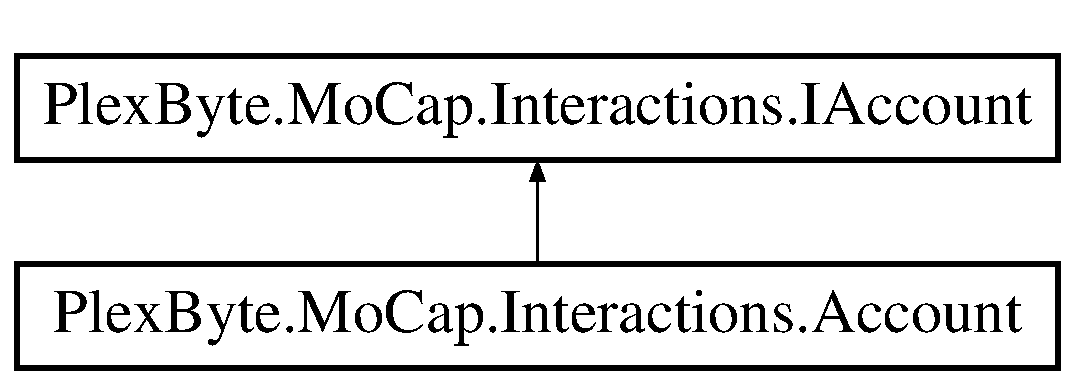
\includegraphics[height=2.000000cm]{interface_plex_byte_1_1_mo_cap_1_1_interactions_1_1_i_account}
\end{center}
\end{figure}
\subsection*{Public Member Functions}
\begin{DoxyCompactItemize}
\item 
void \hyperlink{interface_plex_byte_1_1_mo_cap_1_1_interactions_1_1_i_account_a824d1d5e807efd91b8b5297c17615181}{Add\+Expense} (\hyperlink{interface_plex_byte_1_1_mo_cap_1_1_interactions_1_1_i_expense}{I\+Expense} p\+Expense)
\item 
void \hyperlink{interface_plex_byte_1_1_mo_cap_1_1_interactions_1_1_i_account_a32338193fc2a47546efe36dc370b6c1a}{Add\+Timeslice} (\hyperlink{interface_plex_byte_1_1_mo_cap_1_1_interactions_1_1_i_timeslice}{I\+Timeslice} p\+Timeslice)
\item 
void \hyperlink{interface_plex_byte_1_1_mo_cap_1_1_interactions_1_1_i_account_aa16e3839c2d7eeb4b18dd883ba913533}{Delete\+Expense} (\hyperlink{interface_plex_byte_1_1_mo_cap_1_1_interactions_1_1_i_expense}{I\+Expense} p\+Expense)
\item 
void \hyperlink{interface_plex_byte_1_1_mo_cap_1_1_interactions_1_1_i_account_ad71ce3f0f04ba8c3563a2e7d1b53378d}{Edit\+Timeslice} (\hyperlink{interface_plex_byte_1_1_mo_cap_1_1_interactions_1_1_i_timeslice}{I\+Timeslice} p\+Timeslice, \hyperlink{interface_plex_byte_1_1_mo_cap_1_1_interactions_1_1_i_timeslice}{I\+Timeslice} p\+New\+Timeslice)
\item 
void \hyperlink{interface_plex_byte_1_1_mo_cap_1_1_interactions_1_1_i_account_a28f21a9fd3584256cc0f5eeb41477e06}{Delete\+Timeslice} (\hyperlink{interface_plex_byte_1_1_mo_cap_1_1_interactions_1_1_i_timeslice}{I\+Timeslice} p\+Timeslice)
\item 
decimal \hyperlink{interface_plex_byte_1_1_mo_cap_1_1_interactions_1_1_i_account_a4a1424e01898012e5457d777006b2a49}{User\+Expense} (I\+User p\+User)
\item 
int \hyperlink{interface_plex_byte_1_1_mo_cap_1_1_interactions_1_1_i_account_a75c8a9171f868234d85ced97117b1b8b}{User\+Timeslice} (I\+User p\+User)
\end{DoxyCompactItemize}
\subsection*{Properties}
\begin{DoxyCompactItemize}
\item 
string \hyperlink{interface_plex_byte_1_1_mo_cap_1_1_interactions_1_1_i_account_a5f3422d283ccd4a4913fcba8863fe675}{Id}\hspace{0.3cm}{\ttfamily  \mbox{[}get\mbox{]}}
\item 
List$<$ \hyperlink{interface_plex_byte_1_1_mo_cap_1_1_interactions_1_1_i_expense}{I\+Expense} $>$ \hyperlink{interface_plex_byte_1_1_mo_cap_1_1_interactions_1_1_i_account_ab720da432a5eaf3f694b7914569dd8c7}{Expense\+List}\hspace{0.3cm}{\ttfamily  \mbox{[}get\mbox{]}}
\item 
List$<$ \hyperlink{interface_plex_byte_1_1_mo_cap_1_1_interactions_1_1_i_timeslice}{I\+Timeslice} $>$ \hyperlink{interface_plex_byte_1_1_mo_cap_1_1_interactions_1_1_i_account_a34e6de5df73fd44aa61cfd2492660ed0}{Timeslice\+List}\hspace{0.3cm}{\ttfamily  \mbox{[}get\mbox{]}}
\end{DoxyCompactItemize}
\subsection*{Events}
\begin{DoxyCompactItemize}
\item 
\hyperlink{namespace_plex_byte_1_1_mo_cap_1_1_interactions_a7c03c08c6f524b34193985c455985f1f}{Expense\+Add} \hyperlink{interface_plex_byte_1_1_mo_cap_1_1_interactions_1_1_i_account_a47d037273f3fb8a3a17581b2c243226a}{Expense\+Added}
\item 
\hyperlink{namespace_plex_byte_1_1_mo_cap_1_1_interactions_a600557b92ababd90f6a91c524998565a}{Timeslice\+Add} \hyperlink{interface_plex_byte_1_1_mo_cap_1_1_interactions_1_1_i_account_a7866018e22c1935e5042e418360f855f}{Timeslice\+Added}
\end{DoxyCompactItemize}


\subsection{Detailed Description}


Definition at line 13 of file I\+Account.\+cs.



\subsection{Member Function Documentation}
\index{Plex\+Byte\+::\+Mo\+Cap\+::\+Interactions\+::\+I\+Account@{Plex\+Byte\+::\+Mo\+Cap\+::\+Interactions\+::\+I\+Account}!Add\+Expense@{Add\+Expense}}
\index{Add\+Expense@{Add\+Expense}!Plex\+Byte\+::\+Mo\+Cap\+::\+Interactions\+::\+I\+Account@{Plex\+Byte\+::\+Mo\+Cap\+::\+Interactions\+::\+I\+Account}}
\subsubsection[{\texorpdfstring{Add\+Expense(\+I\+Expense p\+Expense)}{AddExpense(IExpense pExpense)}}]{\setlength{\rightskip}{0pt plus 5cm}void Plex\+Byte.\+Mo\+Cap.\+Interactions.\+I\+Account.\+Add\+Expense (
\begin{DoxyParamCaption}
\item[{{\bf I\+Expense}}]{p\+Expense}
\end{DoxyParamCaption}
)}\hypertarget{interface_plex_byte_1_1_mo_cap_1_1_interactions_1_1_i_account_a824d1d5e807efd91b8b5297c17615181}{}\label{interface_plex_byte_1_1_mo_cap_1_1_interactions_1_1_i_account_a824d1d5e807efd91b8b5297c17615181}


Implemented in \hyperlink{class_plex_byte_1_1_mo_cap_1_1_interactions_1_1_account_a0f69931bd1d21cb3692f0f08918247bd}{Plex\+Byte.\+Mo\+Cap.\+Interactions.\+Account}.

\index{Plex\+Byte\+::\+Mo\+Cap\+::\+Interactions\+::\+I\+Account@{Plex\+Byte\+::\+Mo\+Cap\+::\+Interactions\+::\+I\+Account}!Add\+Timeslice@{Add\+Timeslice}}
\index{Add\+Timeslice@{Add\+Timeslice}!Plex\+Byte\+::\+Mo\+Cap\+::\+Interactions\+::\+I\+Account@{Plex\+Byte\+::\+Mo\+Cap\+::\+Interactions\+::\+I\+Account}}
\subsubsection[{\texorpdfstring{Add\+Timeslice(\+I\+Timeslice p\+Timeslice)}{AddTimeslice(ITimeslice pTimeslice)}}]{\setlength{\rightskip}{0pt plus 5cm}void Plex\+Byte.\+Mo\+Cap.\+Interactions.\+I\+Account.\+Add\+Timeslice (
\begin{DoxyParamCaption}
\item[{{\bf I\+Timeslice}}]{p\+Timeslice}
\end{DoxyParamCaption}
)}\hypertarget{interface_plex_byte_1_1_mo_cap_1_1_interactions_1_1_i_account_a32338193fc2a47546efe36dc370b6c1a}{}\label{interface_plex_byte_1_1_mo_cap_1_1_interactions_1_1_i_account_a32338193fc2a47546efe36dc370b6c1a}


Implemented in \hyperlink{class_plex_byte_1_1_mo_cap_1_1_interactions_1_1_account_a28d01e56bb3fc78f30f4ed5f259c0e17}{Plex\+Byte.\+Mo\+Cap.\+Interactions.\+Account}.

\index{Plex\+Byte\+::\+Mo\+Cap\+::\+Interactions\+::\+I\+Account@{Plex\+Byte\+::\+Mo\+Cap\+::\+Interactions\+::\+I\+Account}!Delete\+Expense@{Delete\+Expense}}
\index{Delete\+Expense@{Delete\+Expense}!Plex\+Byte\+::\+Mo\+Cap\+::\+Interactions\+::\+I\+Account@{Plex\+Byte\+::\+Mo\+Cap\+::\+Interactions\+::\+I\+Account}}
\subsubsection[{\texorpdfstring{Delete\+Expense(\+I\+Expense p\+Expense)}{DeleteExpense(IExpense pExpense)}}]{\setlength{\rightskip}{0pt plus 5cm}void Plex\+Byte.\+Mo\+Cap.\+Interactions.\+I\+Account.\+Delete\+Expense (
\begin{DoxyParamCaption}
\item[{{\bf I\+Expense}}]{p\+Expense}
\end{DoxyParamCaption}
)}\hypertarget{interface_plex_byte_1_1_mo_cap_1_1_interactions_1_1_i_account_aa16e3839c2d7eeb4b18dd883ba913533}{}\label{interface_plex_byte_1_1_mo_cap_1_1_interactions_1_1_i_account_aa16e3839c2d7eeb4b18dd883ba913533}


Implemented in \hyperlink{class_plex_byte_1_1_mo_cap_1_1_interactions_1_1_account_a84d71e01b4a2a2483b52bc67635499ed}{Plex\+Byte.\+Mo\+Cap.\+Interactions.\+Account}.

\index{Plex\+Byte\+::\+Mo\+Cap\+::\+Interactions\+::\+I\+Account@{Plex\+Byte\+::\+Mo\+Cap\+::\+Interactions\+::\+I\+Account}!Delete\+Timeslice@{Delete\+Timeslice}}
\index{Delete\+Timeslice@{Delete\+Timeslice}!Plex\+Byte\+::\+Mo\+Cap\+::\+Interactions\+::\+I\+Account@{Plex\+Byte\+::\+Mo\+Cap\+::\+Interactions\+::\+I\+Account}}
\subsubsection[{\texorpdfstring{Delete\+Timeslice(\+I\+Timeslice p\+Timeslice)}{DeleteTimeslice(ITimeslice pTimeslice)}}]{\setlength{\rightskip}{0pt plus 5cm}void Plex\+Byte.\+Mo\+Cap.\+Interactions.\+I\+Account.\+Delete\+Timeslice (
\begin{DoxyParamCaption}
\item[{{\bf I\+Timeslice}}]{p\+Timeslice}
\end{DoxyParamCaption}
)}\hypertarget{interface_plex_byte_1_1_mo_cap_1_1_interactions_1_1_i_account_a28f21a9fd3584256cc0f5eeb41477e06}{}\label{interface_plex_byte_1_1_mo_cap_1_1_interactions_1_1_i_account_a28f21a9fd3584256cc0f5eeb41477e06}


Implemented in \hyperlink{class_plex_byte_1_1_mo_cap_1_1_interactions_1_1_account_a8b8d09b65d60431bdbbef7d3aed6a72b}{Plex\+Byte.\+Mo\+Cap.\+Interactions.\+Account}.

\index{Plex\+Byte\+::\+Mo\+Cap\+::\+Interactions\+::\+I\+Account@{Plex\+Byte\+::\+Mo\+Cap\+::\+Interactions\+::\+I\+Account}!Edit\+Timeslice@{Edit\+Timeslice}}
\index{Edit\+Timeslice@{Edit\+Timeslice}!Plex\+Byte\+::\+Mo\+Cap\+::\+Interactions\+::\+I\+Account@{Plex\+Byte\+::\+Mo\+Cap\+::\+Interactions\+::\+I\+Account}}
\subsubsection[{\texorpdfstring{Edit\+Timeslice(\+I\+Timeslice p\+Timeslice, I\+Timeslice p\+New\+Timeslice)}{EditTimeslice(ITimeslice pTimeslice, ITimeslice pNewTimeslice)}}]{\setlength{\rightskip}{0pt plus 5cm}void Plex\+Byte.\+Mo\+Cap.\+Interactions.\+I\+Account.\+Edit\+Timeslice (
\begin{DoxyParamCaption}
\item[{{\bf I\+Timeslice}}]{p\+Timeslice, }
\item[{{\bf I\+Timeslice}}]{p\+New\+Timeslice}
\end{DoxyParamCaption}
)}\hypertarget{interface_plex_byte_1_1_mo_cap_1_1_interactions_1_1_i_account_ad71ce3f0f04ba8c3563a2e7d1b53378d}{}\label{interface_plex_byte_1_1_mo_cap_1_1_interactions_1_1_i_account_ad71ce3f0f04ba8c3563a2e7d1b53378d}


Implemented in \hyperlink{class_plex_byte_1_1_mo_cap_1_1_interactions_1_1_account_a3baea063609ff894849c852c249a3c7a}{Plex\+Byte.\+Mo\+Cap.\+Interactions.\+Account}.

\index{Plex\+Byte\+::\+Mo\+Cap\+::\+Interactions\+::\+I\+Account@{Plex\+Byte\+::\+Mo\+Cap\+::\+Interactions\+::\+I\+Account}!User\+Expense@{User\+Expense}}
\index{User\+Expense@{User\+Expense}!Plex\+Byte\+::\+Mo\+Cap\+::\+Interactions\+::\+I\+Account@{Plex\+Byte\+::\+Mo\+Cap\+::\+Interactions\+::\+I\+Account}}
\subsubsection[{\texorpdfstring{User\+Expense(\+I\+User p\+User)}{UserExpense(IUser pUser)}}]{\setlength{\rightskip}{0pt plus 5cm}decimal Plex\+Byte.\+Mo\+Cap.\+Interactions.\+I\+Account.\+User\+Expense (
\begin{DoxyParamCaption}
\item[{I\+User}]{p\+User}
\end{DoxyParamCaption}
)}\hypertarget{interface_plex_byte_1_1_mo_cap_1_1_interactions_1_1_i_account_a4a1424e01898012e5457d777006b2a49}{}\label{interface_plex_byte_1_1_mo_cap_1_1_interactions_1_1_i_account_a4a1424e01898012e5457d777006b2a49}


Implemented in \hyperlink{class_plex_byte_1_1_mo_cap_1_1_interactions_1_1_account_a44cddcf32dbd3ce31fc012104f25e9f8}{Plex\+Byte.\+Mo\+Cap.\+Interactions.\+Account}.

\index{Plex\+Byte\+::\+Mo\+Cap\+::\+Interactions\+::\+I\+Account@{Plex\+Byte\+::\+Mo\+Cap\+::\+Interactions\+::\+I\+Account}!User\+Timeslice@{User\+Timeslice}}
\index{User\+Timeslice@{User\+Timeslice}!Plex\+Byte\+::\+Mo\+Cap\+::\+Interactions\+::\+I\+Account@{Plex\+Byte\+::\+Mo\+Cap\+::\+Interactions\+::\+I\+Account}}
\subsubsection[{\texorpdfstring{User\+Timeslice(\+I\+User p\+User)}{UserTimeslice(IUser pUser)}}]{\setlength{\rightskip}{0pt plus 5cm}int Plex\+Byte.\+Mo\+Cap.\+Interactions.\+I\+Account.\+User\+Timeslice (
\begin{DoxyParamCaption}
\item[{I\+User}]{p\+User}
\end{DoxyParamCaption}
)}\hypertarget{interface_plex_byte_1_1_mo_cap_1_1_interactions_1_1_i_account_a75c8a9171f868234d85ced97117b1b8b}{}\label{interface_plex_byte_1_1_mo_cap_1_1_interactions_1_1_i_account_a75c8a9171f868234d85ced97117b1b8b}


Implemented in \hyperlink{class_plex_byte_1_1_mo_cap_1_1_interactions_1_1_account_a77706a7728657fb56f5f5dc85bd738f4}{Plex\+Byte.\+Mo\+Cap.\+Interactions.\+Account}.



\subsection{Property Documentation}
\index{Plex\+Byte\+::\+Mo\+Cap\+::\+Interactions\+::\+I\+Account@{Plex\+Byte\+::\+Mo\+Cap\+::\+Interactions\+::\+I\+Account}!Expense\+List@{Expense\+List}}
\index{Expense\+List@{Expense\+List}!Plex\+Byte\+::\+Mo\+Cap\+::\+Interactions\+::\+I\+Account@{Plex\+Byte\+::\+Mo\+Cap\+::\+Interactions\+::\+I\+Account}}
\subsubsection[{\texorpdfstring{Expense\+List}{ExpenseList}}]{\setlength{\rightskip}{0pt plus 5cm}List$<${\bf I\+Expense}$>$ Plex\+Byte.\+Mo\+Cap.\+Interactions.\+I\+Account.\+Expense\+List\hspace{0.3cm}{\ttfamily [get]}}\hypertarget{interface_plex_byte_1_1_mo_cap_1_1_interactions_1_1_i_account_ab720da432a5eaf3f694b7914569dd8c7}{}\label{interface_plex_byte_1_1_mo_cap_1_1_interactions_1_1_i_account_ab720da432a5eaf3f694b7914569dd8c7}


Definition at line 21 of file I\+Account.\+cs.

\index{Plex\+Byte\+::\+Mo\+Cap\+::\+Interactions\+::\+I\+Account@{Plex\+Byte\+::\+Mo\+Cap\+::\+Interactions\+::\+I\+Account}!Id@{Id}}
\index{Id@{Id}!Plex\+Byte\+::\+Mo\+Cap\+::\+Interactions\+::\+I\+Account@{Plex\+Byte\+::\+Mo\+Cap\+::\+Interactions\+::\+I\+Account}}
\subsubsection[{\texorpdfstring{Id}{Id}}]{\setlength{\rightskip}{0pt plus 5cm}string Plex\+Byte.\+Mo\+Cap.\+Interactions.\+I\+Account.\+Id\hspace{0.3cm}{\ttfamily [get]}}\hypertarget{interface_plex_byte_1_1_mo_cap_1_1_interactions_1_1_i_account_a5f3422d283ccd4a4913fcba8863fe675}{}\label{interface_plex_byte_1_1_mo_cap_1_1_interactions_1_1_i_account_a5f3422d283ccd4a4913fcba8863fe675}


Definition at line 19 of file I\+Account.\+cs.

\index{Plex\+Byte\+::\+Mo\+Cap\+::\+Interactions\+::\+I\+Account@{Plex\+Byte\+::\+Mo\+Cap\+::\+Interactions\+::\+I\+Account}!Timeslice\+List@{Timeslice\+List}}
\index{Timeslice\+List@{Timeslice\+List}!Plex\+Byte\+::\+Mo\+Cap\+::\+Interactions\+::\+I\+Account@{Plex\+Byte\+::\+Mo\+Cap\+::\+Interactions\+::\+I\+Account}}
\subsubsection[{\texorpdfstring{Timeslice\+List}{TimesliceList}}]{\setlength{\rightskip}{0pt plus 5cm}List$<${\bf I\+Timeslice}$>$ Plex\+Byte.\+Mo\+Cap.\+Interactions.\+I\+Account.\+Timeslice\+List\hspace{0.3cm}{\ttfamily [get]}}\hypertarget{interface_plex_byte_1_1_mo_cap_1_1_interactions_1_1_i_account_a34e6de5df73fd44aa61cfd2492660ed0}{}\label{interface_plex_byte_1_1_mo_cap_1_1_interactions_1_1_i_account_a34e6de5df73fd44aa61cfd2492660ed0}


Definition at line 23 of file I\+Account.\+cs.



\subsection{Event Documentation}
\index{Plex\+Byte\+::\+Mo\+Cap\+::\+Interactions\+::\+I\+Account@{Plex\+Byte\+::\+Mo\+Cap\+::\+Interactions\+::\+I\+Account}!Expense\+Added@{Expense\+Added}}
\index{Expense\+Added@{Expense\+Added}!Plex\+Byte\+::\+Mo\+Cap\+::\+Interactions\+::\+I\+Account@{Plex\+Byte\+::\+Mo\+Cap\+::\+Interactions\+::\+I\+Account}}
\subsubsection[{\texorpdfstring{Expense\+Added}{ExpenseAdded}}]{\setlength{\rightskip}{0pt plus 5cm}{\bf Expense\+Add} Plex\+Byte.\+Mo\+Cap.\+Interactions.\+I\+Account.\+Expense\+Added}\hypertarget{interface_plex_byte_1_1_mo_cap_1_1_interactions_1_1_i_account_a47d037273f3fb8a3a17581b2c243226a}{}\label{interface_plex_byte_1_1_mo_cap_1_1_interactions_1_1_i_account_a47d037273f3fb8a3a17581b2c243226a}


Definition at line 15 of file I\+Account.\+cs.

\index{Plex\+Byte\+::\+Mo\+Cap\+::\+Interactions\+::\+I\+Account@{Plex\+Byte\+::\+Mo\+Cap\+::\+Interactions\+::\+I\+Account}!Timeslice\+Added@{Timeslice\+Added}}
\index{Timeslice\+Added@{Timeslice\+Added}!Plex\+Byte\+::\+Mo\+Cap\+::\+Interactions\+::\+I\+Account@{Plex\+Byte\+::\+Mo\+Cap\+::\+Interactions\+::\+I\+Account}}
\subsubsection[{\texorpdfstring{Timeslice\+Added}{TimesliceAdded}}]{\setlength{\rightskip}{0pt plus 5cm}{\bf Timeslice\+Add} Plex\+Byte.\+Mo\+Cap.\+Interactions.\+I\+Account.\+Timeslice\+Added}\hypertarget{interface_plex_byte_1_1_mo_cap_1_1_interactions_1_1_i_account_a7866018e22c1935e5042e418360f855f}{}\label{interface_plex_byte_1_1_mo_cap_1_1_interactions_1_1_i_account_a7866018e22c1935e5042e418360f855f}


Definition at line 16 of file I\+Account.\+cs.



The documentation for this interface was generated from the following file\+:\begin{DoxyCompactItemize}
\item 
D\+:/\+Users/\+Christian\+B/\+Documents/\+\_\+\+H\+F Infomatik/\+Git\+Hub\+\_\+\+Repos/\+Mo\+Cap/\+Plex\+Byte.\+Mo\+Cap/\+Plex\+Byte.\+Mo\+Cap.\+Interactions/\hyperlink{_i_account_8cs}{I\+Account.\+cs}\end{DoxyCompactItemize}

\hypertarget{interface_plex_byte_1_1_mo_cap_1_1_interactions_1_1_i_expense}{}\section{Plex\+Byte.\+Mo\+Cap.\+Interactions.\+I\+Expense Interface Reference}
\label{interface_plex_byte_1_1_mo_cap_1_1_interactions_1_1_i_expense}\index{Plex\+Byte.\+Mo\+Cap.\+Interactions.\+I\+Expense@{Plex\+Byte.\+Mo\+Cap.\+Interactions.\+I\+Expense}}
Inheritance diagram for Plex\+Byte.\+Mo\+Cap.\+Interactions.\+I\+Expense\+:\begin{figure}[H]
\begin{center}
\leavevmode
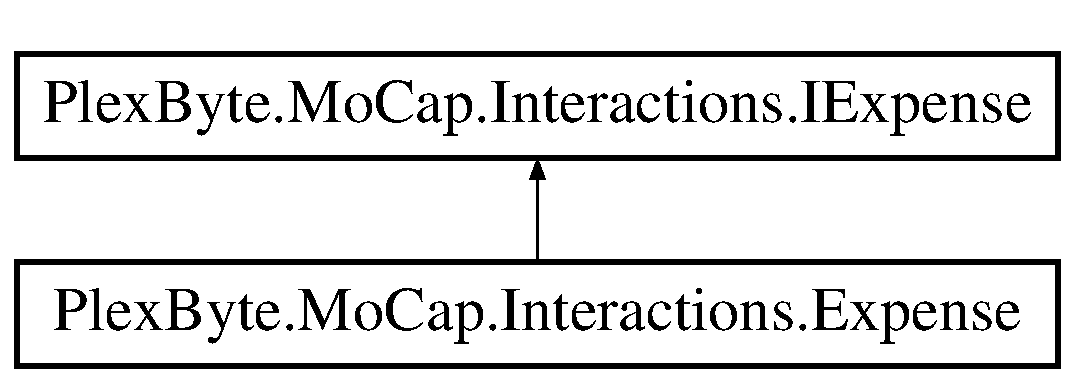
\includegraphics[height=2.000000cm]{interface_plex_byte_1_1_mo_cap_1_1_interactions_1_1_i_expense}
\end{center}
\end{figure}
\subsection*{Public Member Functions}
\begin{DoxyCompactItemize}
\item 
void \hyperlink{interface_plex_byte_1_1_mo_cap_1_1_interactions_1_1_i_expense_a8c87ed5e40ba6397f7c7a6b68fea9b01}{Add\+Receipt} (Image p\+Receipt)
\item 
void \hyperlink{interface_plex_byte_1_1_mo_cap_1_1_interactions_1_1_i_expense_ae5c1051bde332fa436e8521070424965}{Delete\+Receipt} ()
\item 
void \hyperlink{interface_plex_byte_1_1_mo_cap_1_1_interactions_1_1_i_expense_aba0d437cd05e76e67fc0cf544c54d85e}{Edit\+Value} (decimal p\+New\+Value)
\end{DoxyCompactItemize}
\subsection*{Properties}
\begin{DoxyCompactItemize}
\item 
decimal \hyperlink{interface_plex_byte_1_1_mo_cap_1_1_interactions_1_1_i_expense_aca2002cb7567125addc9064daed1d95a}{Value}\hspace{0.3cm}{\ttfamily  \mbox{[}get\mbox{]}}
\item 
System.\+Drawing.\+Image \hyperlink{interface_plex_byte_1_1_mo_cap_1_1_interactions_1_1_i_expense_a164199a26cd05415a6075b64a428d64f}{Receipt}\hspace{0.3cm}{\ttfamily  \mbox{[}get\mbox{]}}
\item 
\hyperlink{interface_plex_byte_1_1_mo_cap_1_1_interactions_1_1_i_interaction}{I\+Interaction} \hyperlink{interface_plex_byte_1_1_mo_cap_1_1_interactions_1_1_i_expense_ad33b05045db2c97941e9e16ae6e643f5}{Target}\hspace{0.3cm}{\ttfamily  \mbox{[}get\mbox{]}}
\item 
I\+User \hyperlink{interface_plex_byte_1_1_mo_cap_1_1_interactions_1_1_i_expense_a3982207fd0c476dae28597cd163de03d}{User}\hspace{0.3cm}{\ttfamily  \mbox{[}get\mbox{]}}
\end{DoxyCompactItemize}


\subsection{Detailed Description}


Definition at line 9 of file I\+Expense.\+cs.



\subsection{Member Function Documentation}
\index{Plex\+Byte\+::\+Mo\+Cap\+::\+Interactions\+::\+I\+Expense@{Plex\+Byte\+::\+Mo\+Cap\+::\+Interactions\+::\+I\+Expense}!Add\+Receipt@{Add\+Receipt}}
\index{Add\+Receipt@{Add\+Receipt}!Plex\+Byte\+::\+Mo\+Cap\+::\+Interactions\+::\+I\+Expense@{Plex\+Byte\+::\+Mo\+Cap\+::\+Interactions\+::\+I\+Expense}}
\subsubsection[{\texorpdfstring{Add\+Receipt(\+Image p\+Receipt)}{AddReceipt(Image pReceipt)}}]{\setlength{\rightskip}{0pt plus 5cm}void Plex\+Byte.\+Mo\+Cap.\+Interactions.\+I\+Expense.\+Add\+Receipt (
\begin{DoxyParamCaption}
\item[{Image}]{p\+Receipt}
\end{DoxyParamCaption}
)}\hypertarget{interface_plex_byte_1_1_mo_cap_1_1_interactions_1_1_i_expense_a8c87ed5e40ba6397f7c7a6b68fea9b01}{}\label{interface_plex_byte_1_1_mo_cap_1_1_interactions_1_1_i_expense_a8c87ed5e40ba6397f7c7a6b68fea9b01}


Implemented in \hyperlink{class_plex_byte_1_1_mo_cap_1_1_interactions_1_1_expense_a33e21b15e70fa450463a5a5197dcfe38}{Plex\+Byte.\+Mo\+Cap.\+Interactions.\+Expense}.

\index{Plex\+Byte\+::\+Mo\+Cap\+::\+Interactions\+::\+I\+Expense@{Plex\+Byte\+::\+Mo\+Cap\+::\+Interactions\+::\+I\+Expense}!Delete\+Receipt@{Delete\+Receipt}}
\index{Delete\+Receipt@{Delete\+Receipt}!Plex\+Byte\+::\+Mo\+Cap\+::\+Interactions\+::\+I\+Expense@{Plex\+Byte\+::\+Mo\+Cap\+::\+Interactions\+::\+I\+Expense}}
\subsubsection[{\texorpdfstring{Delete\+Receipt()}{DeleteReceipt()}}]{\setlength{\rightskip}{0pt plus 5cm}void Plex\+Byte.\+Mo\+Cap.\+Interactions.\+I\+Expense.\+Delete\+Receipt (
\begin{DoxyParamCaption}
{}
\end{DoxyParamCaption}
)}\hypertarget{interface_plex_byte_1_1_mo_cap_1_1_interactions_1_1_i_expense_ae5c1051bde332fa436e8521070424965}{}\label{interface_plex_byte_1_1_mo_cap_1_1_interactions_1_1_i_expense_ae5c1051bde332fa436e8521070424965}


Implemented in \hyperlink{class_plex_byte_1_1_mo_cap_1_1_interactions_1_1_expense_a927ad9089c43c09790083d554b1139f8}{Plex\+Byte.\+Mo\+Cap.\+Interactions.\+Expense}.

\index{Plex\+Byte\+::\+Mo\+Cap\+::\+Interactions\+::\+I\+Expense@{Plex\+Byte\+::\+Mo\+Cap\+::\+Interactions\+::\+I\+Expense}!Edit\+Value@{Edit\+Value}}
\index{Edit\+Value@{Edit\+Value}!Plex\+Byte\+::\+Mo\+Cap\+::\+Interactions\+::\+I\+Expense@{Plex\+Byte\+::\+Mo\+Cap\+::\+Interactions\+::\+I\+Expense}}
\subsubsection[{\texorpdfstring{Edit\+Value(decimal p\+New\+Value)}{EditValue(decimal pNewValue)}}]{\setlength{\rightskip}{0pt plus 5cm}void Plex\+Byte.\+Mo\+Cap.\+Interactions.\+I\+Expense.\+Edit\+Value (
\begin{DoxyParamCaption}
\item[{decimal}]{p\+New\+Value}
\end{DoxyParamCaption}
)}\hypertarget{interface_plex_byte_1_1_mo_cap_1_1_interactions_1_1_i_expense_aba0d437cd05e76e67fc0cf544c54d85e}{}\label{interface_plex_byte_1_1_mo_cap_1_1_interactions_1_1_i_expense_aba0d437cd05e76e67fc0cf544c54d85e}


Implemented in \hyperlink{class_plex_byte_1_1_mo_cap_1_1_interactions_1_1_expense_ace1f3d1404f02fb78583b1709641c2c1}{Plex\+Byte.\+Mo\+Cap.\+Interactions.\+Expense}.



\subsection{Property Documentation}
\index{Plex\+Byte\+::\+Mo\+Cap\+::\+Interactions\+::\+I\+Expense@{Plex\+Byte\+::\+Mo\+Cap\+::\+Interactions\+::\+I\+Expense}!Receipt@{Receipt}}
\index{Receipt@{Receipt}!Plex\+Byte\+::\+Mo\+Cap\+::\+Interactions\+::\+I\+Expense@{Plex\+Byte\+::\+Mo\+Cap\+::\+Interactions\+::\+I\+Expense}}
\subsubsection[{\texorpdfstring{Receipt}{Receipt}}]{\setlength{\rightskip}{0pt plus 5cm}System.\+Drawing.\+Image Plex\+Byte.\+Mo\+Cap.\+Interactions.\+I\+Expense.\+Receipt\hspace{0.3cm}{\ttfamily [get]}}\hypertarget{interface_plex_byte_1_1_mo_cap_1_1_interactions_1_1_i_expense_a164199a26cd05415a6075b64a428d64f}{}\label{interface_plex_byte_1_1_mo_cap_1_1_interactions_1_1_i_expense_a164199a26cd05415a6075b64a428d64f}


Definition at line 13 of file I\+Expense.\+cs.

\index{Plex\+Byte\+::\+Mo\+Cap\+::\+Interactions\+::\+I\+Expense@{Plex\+Byte\+::\+Mo\+Cap\+::\+Interactions\+::\+I\+Expense}!Target@{Target}}
\index{Target@{Target}!Plex\+Byte\+::\+Mo\+Cap\+::\+Interactions\+::\+I\+Expense@{Plex\+Byte\+::\+Mo\+Cap\+::\+Interactions\+::\+I\+Expense}}
\subsubsection[{\texorpdfstring{Target}{Target}}]{\setlength{\rightskip}{0pt plus 5cm}{\bf I\+Interaction} Plex\+Byte.\+Mo\+Cap.\+Interactions.\+I\+Expense.\+Target\hspace{0.3cm}{\ttfamily [get]}}\hypertarget{interface_plex_byte_1_1_mo_cap_1_1_interactions_1_1_i_expense_ad33b05045db2c97941e9e16ae6e643f5}{}\label{interface_plex_byte_1_1_mo_cap_1_1_interactions_1_1_i_expense_ad33b05045db2c97941e9e16ae6e643f5}


Definition at line 15 of file I\+Expense.\+cs.

\index{Plex\+Byte\+::\+Mo\+Cap\+::\+Interactions\+::\+I\+Expense@{Plex\+Byte\+::\+Mo\+Cap\+::\+Interactions\+::\+I\+Expense}!User@{User}}
\index{User@{User}!Plex\+Byte\+::\+Mo\+Cap\+::\+Interactions\+::\+I\+Expense@{Plex\+Byte\+::\+Mo\+Cap\+::\+Interactions\+::\+I\+Expense}}
\subsubsection[{\texorpdfstring{User}{User}}]{\setlength{\rightskip}{0pt plus 5cm}I\+User Plex\+Byte.\+Mo\+Cap.\+Interactions.\+I\+Expense.\+User\hspace{0.3cm}{\ttfamily [get]}}\hypertarget{interface_plex_byte_1_1_mo_cap_1_1_interactions_1_1_i_expense_a3982207fd0c476dae28597cd163de03d}{}\label{interface_plex_byte_1_1_mo_cap_1_1_interactions_1_1_i_expense_a3982207fd0c476dae28597cd163de03d}


Definition at line 17 of file I\+Expense.\+cs.

\index{Plex\+Byte\+::\+Mo\+Cap\+::\+Interactions\+::\+I\+Expense@{Plex\+Byte\+::\+Mo\+Cap\+::\+Interactions\+::\+I\+Expense}!Value@{Value}}
\index{Value@{Value}!Plex\+Byte\+::\+Mo\+Cap\+::\+Interactions\+::\+I\+Expense@{Plex\+Byte\+::\+Mo\+Cap\+::\+Interactions\+::\+I\+Expense}}
\subsubsection[{\texorpdfstring{Value}{Value}}]{\setlength{\rightskip}{0pt plus 5cm}decimal Plex\+Byte.\+Mo\+Cap.\+Interactions.\+I\+Expense.\+Value\hspace{0.3cm}{\ttfamily [get]}}\hypertarget{interface_plex_byte_1_1_mo_cap_1_1_interactions_1_1_i_expense_aca2002cb7567125addc9064daed1d95a}{}\label{interface_plex_byte_1_1_mo_cap_1_1_interactions_1_1_i_expense_aca2002cb7567125addc9064daed1d95a}


Definition at line 11 of file I\+Expense.\+cs.



The documentation for this interface was generated from the following file\+:\begin{DoxyCompactItemize}
\item 
D\+:/\+Users/\+Christian\+B/\+Documents/\+\_\+\+H\+F Infomatik/\+Git\+Hub\+\_\+\+Repos/\+Mo\+Cap/\+Plex\+Byte.\+Mo\+Cap/\+Plex\+Byte.\+Mo\+Cap.\+Interactions/\hyperlink{_i_expense_8cs}{I\+Expense.\+cs}\end{DoxyCompactItemize}

\hypertarget{interface_plex_byte_1_1_mo_cap_1_1_interactions_1_1_i_interaction}{}\section{Plex\+Byte.\+Mo\+Cap.\+Interactions.\+I\+Interaction Interface Reference}
\label{interface_plex_byte_1_1_mo_cap_1_1_interactions_1_1_i_interaction}\index{Plex\+Byte.\+Mo\+Cap.\+Interactions.\+I\+Interaction@{Plex\+Byte.\+Mo\+Cap.\+Interactions.\+I\+Interaction}}
Inheritance diagram for Plex\+Byte.\+Mo\+Cap.\+Interactions.\+I\+Interaction\+:\begin{figure}[H]
\begin{center}
\leavevmode
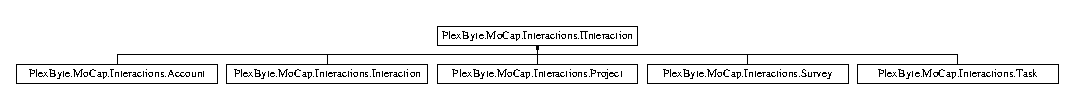
\includegraphics[height=0.899598cm]{interface_plex_byte_1_1_mo_cap_1_1_interactions_1_1_i_interaction}
\end{center}
\end{figure}
\subsection*{Public Member Functions}
\begin{DoxyCompactItemize}
\item 
void \hyperlink{interface_plex_byte_1_1_mo_cap_1_1_interactions_1_1_i_interaction_a9f32d6c1c2f2ae60dabb274f62128447}{On\+Complete} (\hyperlink{class_plex_byte_1_1_mo_cap_1_1_interactions_1_1_interaction_event_args}{Interaction\+Event\+Args} p\+Event\+Args)
\item 
void \hyperlink{interface_plex_byte_1_1_mo_cap_1_1_interactions_1_1_i_interaction_a7e3b0a67dc7d176877b8b94922a9bb52}{Change\+Owner} (I\+User p\+User)
\item 
void \hyperlink{interface_plex_byte_1_1_mo_cap_1_1_interactions_1_1_i_interaction_ac2d9f47a1139b931939e8cff07153aba}{Change\+Is\+Active} (bool p\+Active)
\item 
void \hyperlink{interface_plex_byte_1_1_mo_cap_1_1_interactions_1_1_i_interaction_af4fac42d753ae7f9652541542b8961c6}{On\+Modify} (\hyperlink{class_plex_byte_1_1_mo_cap_1_1_interactions_1_1_interaction_event_args}{Interaction\+Event\+Args} p\+Event\+Args)
\item 
void \hyperlink{interface_plex_byte_1_1_mo_cap_1_1_interactions_1_1_i_interaction_a5250247fb5f22a633e22d7f8dc946c4d}{On\+State\+Changed} (\hyperlink{class_plex_byte_1_1_mo_cap_1_1_interactions_1_1_interaction_event_args}{Interaction\+Event\+Args} p\+Event\+Args)
\item 
void \hyperlink{interface_plex_byte_1_1_mo_cap_1_1_interactions_1_1_i_interaction_a10beb35eb6061878469b5a6cd5431b32}{Change\+State} (\hyperlink{namespace_plex_byte_1_1_mo_cap_1_1_interactions_afcb673d9186608b6bd3b187179aedc8a}{Interaction\+State} p\+State)
\end{DoxyCompactItemize}
\subsection*{Properties}
\begin{DoxyCompactItemize}
\item 
string \hyperlink{interface_plex_byte_1_1_mo_cap_1_1_interactions_1_1_i_interaction_aa3e9cbd6df674752a1746b11c08b9967}{Id}\hspace{0.3cm}{\ttfamily  \mbox{[}get\mbox{]}}
\item 
Date\+Time \hyperlink{interface_plex_byte_1_1_mo_cap_1_1_interactions_1_1_i_interaction_ad7cb75815bcac172e1944418ec2e7e33}{Start\+Date\+Time}\hspace{0.3cm}{\ttfamily  \mbox{[}get, set\mbox{]}}
\item 
Date\+Time \hyperlink{interface_plex_byte_1_1_mo_cap_1_1_interactions_1_1_i_interaction_a555336719848fe4e8e8cec0b651de96e}{End\+Date\+Time}\hspace{0.3cm}{\ttfamily  \mbox{[}get, set\mbox{]}}
\item 
Date\+Time \hyperlink{interface_plex_byte_1_1_mo_cap_1_1_interactions_1_1_i_interaction_ad0df86b8149883cbaa21df6ab2bfa6fc}{Created\+Date\+Time}\hspace{0.3cm}{\ttfamily  \mbox{[}get\mbox{]}}
\item 
Date\+Time \hyperlink{interface_plex_byte_1_1_mo_cap_1_1_interactions_1_1_i_interaction_a4f06f6eef1c8cbdc1f0e1ee48140e17e}{Modified\+Date\+Time}\hspace{0.3cm}{\ttfamily  \mbox{[}get, set\mbox{]}}
\item 
bool \hyperlink{interface_plex_byte_1_1_mo_cap_1_1_interactions_1_1_i_interaction_a6ff177af835714ffd17f27b9016ef131}{Is\+Active}\hspace{0.3cm}{\ttfamily  \mbox{[}get\mbox{]}}
\item 
string \hyperlink{interface_plex_byte_1_1_mo_cap_1_1_interactions_1_1_i_interaction_ab92e9fa8ce447f0468bd4e1fdce4f851}{Text}\hspace{0.3cm}{\ttfamily  \mbox{[}get, set\mbox{]}}
\item 
\hyperlink{namespace_plex_byte_1_1_mo_cap_1_1_interactions_a6e7bea333446664bbce2bb296db25e31}{Interaction\+Type} \hyperlink{interface_plex_byte_1_1_mo_cap_1_1_interactions_1_1_i_interaction_aa8f2e2760f79850529e38d1e84a0a92e}{Type}\hspace{0.3cm}{\ttfamily  \mbox{[}get\mbox{]}}
\item 
I\+User \hyperlink{interface_plex_byte_1_1_mo_cap_1_1_interactions_1_1_i_interaction_a4df2832bccdf71ce16b0eba22e6914f2}{Creator}\hspace{0.3cm}{\ttfamily  \mbox{[}get\mbox{]}}
\item 
I\+User \hyperlink{interface_plex_byte_1_1_mo_cap_1_1_interactions_1_1_i_interaction_aa6fdd0b6da97043e6961ca3ec04e1d94}{Owner}\hspace{0.3cm}{\ttfamily  \mbox{[}get, set\mbox{]}}
\item 
\hyperlink{namespace_plex_byte_1_1_mo_cap_1_1_interactions_afcb673d9186608b6bd3b187179aedc8a}{Interaction\+State} \hyperlink{interface_plex_byte_1_1_mo_cap_1_1_interactions_1_1_i_interaction_a149f0058af52987cef67f429ba756d01}{State}\hspace{0.3cm}{\ttfamily  \mbox{[}get\mbox{]}}
\end{DoxyCompactItemize}
\subsection*{Events}
\begin{DoxyCompactItemize}
\item 
\hyperlink{namespace_plex_byte_1_1_mo_cap_1_1_interactions_ac81ac3321ab2b018c75ad2c18ec15b9e}{Complete} \hyperlink{interface_plex_byte_1_1_mo_cap_1_1_interactions_1_1_i_interaction_a7ebca376ae67dbaab7d8a2659f15aa20}{Completed}
\item 
\hyperlink{namespace_plex_byte_1_1_mo_cap_1_1_interactions_a490186f613e46adce26244f3b2c78a58}{Modify} \hyperlink{interface_plex_byte_1_1_mo_cap_1_1_interactions_1_1_i_interaction_a54b3a6e068719473b4a34d10504766a1}{Modified}
\item 
\hyperlink{namespace_plex_byte_1_1_mo_cap_1_1_interactions_af2ff213e81451f96fc74bfad114cecde}{State\+Change} \hyperlink{interface_plex_byte_1_1_mo_cap_1_1_interactions_1_1_i_interaction_af6cf60a1a30e422da1b7552868c03001}{State\+Changed}
\end{DoxyCompactItemize}


\subsection{Detailed Description}


Definition at line 17 of file I\+Interaction.\+cs.



\subsection{Member Function Documentation}
\index{Plex\+Byte\+::\+Mo\+Cap\+::\+Interactions\+::\+I\+Interaction@{Plex\+Byte\+::\+Mo\+Cap\+::\+Interactions\+::\+I\+Interaction}!Change\+Is\+Active@{Change\+Is\+Active}}
\index{Change\+Is\+Active@{Change\+Is\+Active}!Plex\+Byte\+::\+Mo\+Cap\+::\+Interactions\+::\+I\+Interaction@{Plex\+Byte\+::\+Mo\+Cap\+::\+Interactions\+::\+I\+Interaction}}
\subsubsection[{\texorpdfstring{Change\+Is\+Active(bool p\+Active)}{ChangeIsActive(bool pActive)}}]{\setlength{\rightskip}{0pt plus 5cm}void Plex\+Byte.\+Mo\+Cap.\+Interactions.\+I\+Interaction.\+Change\+Is\+Active (
\begin{DoxyParamCaption}
\item[{bool}]{p\+Active}
\end{DoxyParamCaption}
)}\hypertarget{interface_plex_byte_1_1_mo_cap_1_1_interactions_1_1_i_interaction_ac2d9f47a1139b931939e8cff07153aba}{}\label{interface_plex_byte_1_1_mo_cap_1_1_interactions_1_1_i_interaction_ac2d9f47a1139b931939e8cff07153aba}


Implemented in \hyperlink{class_plex_byte_1_1_mo_cap_1_1_interactions_1_1_project_adcbdd39b8b64051e9bbdfffd25663116}{Plex\+Byte.\+Mo\+Cap.\+Interactions.\+Project}, \hyperlink{class_plex_byte_1_1_mo_cap_1_1_interactions_1_1_task_ae0cb74071fbffd9fa7cd1dba842b6715}{Plex\+Byte.\+Mo\+Cap.\+Interactions.\+Task}, \hyperlink{class_plex_byte_1_1_mo_cap_1_1_interactions_1_1_account_aa599051753ac017c4fa2613fa16be415}{Plex\+Byte.\+Mo\+Cap.\+Interactions.\+Account}, \hyperlink{class_plex_byte_1_1_mo_cap_1_1_interactions_1_1_survey_ab51b78828fafe0eaa305d6c80df91b0f}{Plex\+Byte.\+Mo\+Cap.\+Interactions.\+Survey}, and \hyperlink{class_plex_byte_1_1_mo_cap_1_1_interactions_1_1_interaction_ab58345952cc115beaa62f8e556387b87}{Plex\+Byte.\+Mo\+Cap.\+Interactions.\+Interaction}.

\index{Plex\+Byte\+::\+Mo\+Cap\+::\+Interactions\+::\+I\+Interaction@{Plex\+Byte\+::\+Mo\+Cap\+::\+Interactions\+::\+I\+Interaction}!Change\+Owner@{Change\+Owner}}
\index{Change\+Owner@{Change\+Owner}!Plex\+Byte\+::\+Mo\+Cap\+::\+Interactions\+::\+I\+Interaction@{Plex\+Byte\+::\+Mo\+Cap\+::\+Interactions\+::\+I\+Interaction}}
\subsubsection[{\texorpdfstring{Change\+Owner(\+I\+User p\+User)}{ChangeOwner(IUser pUser)}}]{\setlength{\rightskip}{0pt plus 5cm}void Plex\+Byte.\+Mo\+Cap.\+Interactions.\+I\+Interaction.\+Change\+Owner (
\begin{DoxyParamCaption}
\item[{I\+User}]{p\+User}
\end{DoxyParamCaption}
)}\hypertarget{interface_plex_byte_1_1_mo_cap_1_1_interactions_1_1_i_interaction_a7e3b0a67dc7d176877b8b94922a9bb52}{}\label{interface_plex_byte_1_1_mo_cap_1_1_interactions_1_1_i_interaction_a7e3b0a67dc7d176877b8b94922a9bb52}


Implemented in \hyperlink{class_plex_byte_1_1_mo_cap_1_1_interactions_1_1_project_a4e59d6c532937fb758e055af3fa2da77}{Plex\+Byte.\+Mo\+Cap.\+Interactions.\+Project}, \hyperlink{class_plex_byte_1_1_mo_cap_1_1_interactions_1_1_task_a47eac360e6cf4cd6b84f7445ee4a6a33}{Plex\+Byte.\+Mo\+Cap.\+Interactions.\+Task}, \hyperlink{class_plex_byte_1_1_mo_cap_1_1_interactions_1_1_account_a7220958b8470021790726ae8e68078a5}{Plex\+Byte.\+Mo\+Cap.\+Interactions.\+Account}, \hyperlink{class_plex_byte_1_1_mo_cap_1_1_interactions_1_1_survey_a1c301916ee78db1236c465cd3fe40449}{Plex\+Byte.\+Mo\+Cap.\+Interactions.\+Survey}, and \hyperlink{class_plex_byte_1_1_mo_cap_1_1_interactions_1_1_interaction_a4ef64eb1f5bb5e03d1d5ef5cec52f759}{Plex\+Byte.\+Mo\+Cap.\+Interactions.\+Interaction}.

\index{Plex\+Byte\+::\+Mo\+Cap\+::\+Interactions\+::\+I\+Interaction@{Plex\+Byte\+::\+Mo\+Cap\+::\+Interactions\+::\+I\+Interaction}!Change\+State@{Change\+State}}
\index{Change\+State@{Change\+State}!Plex\+Byte\+::\+Mo\+Cap\+::\+Interactions\+::\+I\+Interaction@{Plex\+Byte\+::\+Mo\+Cap\+::\+Interactions\+::\+I\+Interaction}}
\subsubsection[{\texorpdfstring{Change\+State(\+Interaction\+State p\+State)}{ChangeState(InteractionState pState)}}]{\setlength{\rightskip}{0pt plus 5cm}void Plex\+Byte.\+Mo\+Cap.\+Interactions.\+I\+Interaction.\+Change\+State (
\begin{DoxyParamCaption}
\item[{{\bf Interaction\+State}}]{p\+State}
\end{DoxyParamCaption}
)}\hypertarget{interface_plex_byte_1_1_mo_cap_1_1_interactions_1_1_i_interaction_a10beb35eb6061878469b5a6cd5431b32}{}\label{interface_plex_byte_1_1_mo_cap_1_1_interactions_1_1_i_interaction_a10beb35eb6061878469b5a6cd5431b32}


Implemented in \hyperlink{class_plex_byte_1_1_mo_cap_1_1_interactions_1_1_project_a7a916aeebe04d4dd33765b6127282543}{Plex\+Byte.\+Mo\+Cap.\+Interactions.\+Project}, \hyperlink{class_plex_byte_1_1_mo_cap_1_1_interactions_1_1_task_a42cc4439fb4ab6d4e11f8764b217b46d}{Plex\+Byte.\+Mo\+Cap.\+Interactions.\+Task}, \hyperlink{class_plex_byte_1_1_mo_cap_1_1_interactions_1_1_account_a3dadb5bcabffdec7afad04af7c94e2f0}{Plex\+Byte.\+Mo\+Cap.\+Interactions.\+Account}, \hyperlink{class_plex_byte_1_1_mo_cap_1_1_interactions_1_1_survey_a7f44759a0d2ea7ce7516559fe8a70a94}{Plex\+Byte.\+Mo\+Cap.\+Interactions.\+Survey}, and \hyperlink{class_plex_byte_1_1_mo_cap_1_1_interactions_1_1_interaction_a8a50a69a149da786705b71ee33298afb}{Plex\+Byte.\+Mo\+Cap.\+Interactions.\+Interaction}.

\index{Plex\+Byte\+::\+Mo\+Cap\+::\+Interactions\+::\+I\+Interaction@{Plex\+Byte\+::\+Mo\+Cap\+::\+Interactions\+::\+I\+Interaction}!On\+Complete@{On\+Complete}}
\index{On\+Complete@{On\+Complete}!Plex\+Byte\+::\+Mo\+Cap\+::\+Interactions\+::\+I\+Interaction@{Plex\+Byte\+::\+Mo\+Cap\+::\+Interactions\+::\+I\+Interaction}}
\subsubsection[{\texorpdfstring{On\+Complete(\+Interaction\+Event\+Args p\+Event\+Args)}{OnComplete(InteractionEventArgs pEventArgs)}}]{\setlength{\rightskip}{0pt plus 5cm}void Plex\+Byte.\+Mo\+Cap.\+Interactions.\+I\+Interaction.\+On\+Complete (
\begin{DoxyParamCaption}
\item[{{\bf Interaction\+Event\+Args}}]{p\+Event\+Args}
\end{DoxyParamCaption}
)}\hypertarget{interface_plex_byte_1_1_mo_cap_1_1_interactions_1_1_i_interaction_a9f32d6c1c2f2ae60dabb274f62128447}{}\label{interface_plex_byte_1_1_mo_cap_1_1_interactions_1_1_i_interaction_a9f32d6c1c2f2ae60dabb274f62128447}


Implemented in \hyperlink{class_plex_byte_1_1_mo_cap_1_1_interactions_1_1_task_ab74ee9d89534254215ae13eb91e12227}{Plex\+Byte.\+Mo\+Cap.\+Interactions.\+Task}, \hyperlink{class_plex_byte_1_1_mo_cap_1_1_interactions_1_1_project_a039fdf13ac3d4b2b83cb0f3ce7fb4ca1}{Plex\+Byte.\+Mo\+Cap.\+Interactions.\+Project}, \hyperlink{class_plex_byte_1_1_mo_cap_1_1_interactions_1_1_account_a697e062e9b46c58922cbdce34b8e1574}{Plex\+Byte.\+Mo\+Cap.\+Interactions.\+Account}, \hyperlink{class_plex_byte_1_1_mo_cap_1_1_interactions_1_1_survey_ae9f1ca5ffacd44917eda7458a335cefa}{Plex\+Byte.\+Mo\+Cap.\+Interactions.\+Survey}, and \hyperlink{class_plex_byte_1_1_mo_cap_1_1_interactions_1_1_interaction_a0a837bb8d58f8e2077ba901fadd650a6}{Plex\+Byte.\+Mo\+Cap.\+Interactions.\+Interaction}.

\index{Plex\+Byte\+::\+Mo\+Cap\+::\+Interactions\+::\+I\+Interaction@{Plex\+Byte\+::\+Mo\+Cap\+::\+Interactions\+::\+I\+Interaction}!On\+Modify@{On\+Modify}}
\index{On\+Modify@{On\+Modify}!Plex\+Byte\+::\+Mo\+Cap\+::\+Interactions\+::\+I\+Interaction@{Plex\+Byte\+::\+Mo\+Cap\+::\+Interactions\+::\+I\+Interaction}}
\subsubsection[{\texorpdfstring{On\+Modify(\+Interaction\+Event\+Args p\+Event\+Args)}{OnModify(InteractionEventArgs pEventArgs)}}]{\setlength{\rightskip}{0pt plus 5cm}void Plex\+Byte.\+Mo\+Cap.\+Interactions.\+I\+Interaction.\+On\+Modify (
\begin{DoxyParamCaption}
\item[{{\bf Interaction\+Event\+Args}}]{p\+Event\+Args}
\end{DoxyParamCaption}
)}\hypertarget{interface_plex_byte_1_1_mo_cap_1_1_interactions_1_1_i_interaction_af4fac42d753ae7f9652541542b8961c6}{}\label{interface_plex_byte_1_1_mo_cap_1_1_interactions_1_1_i_interaction_af4fac42d753ae7f9652541542b8961c6}


Implemented in \hyperlink{class_plex_byte_1_1_mo_cap_1_1_interactions_1_1_task_ae9e732dc2f41a35a77dd8e143c8cf9c7}{Plex\+Byte.\+Mo\+Cap.\+Interactions.\+Task}, \hyperlink{class_plex_byte_1_1_mo_cap_1_1_interactions_1_1_project_a3255cca2b9dbe1fc60a39463d33a9c31}{Plex\+Byte.\+Mo\+Cap.\+Interactions.\+Project}, \hyperlink{class_plex_byte_1_1_mo_cap_1_1_interactions_1_1_account_a8b3878783c7aa0648adc8633e98e7f4e}{Plex\+Byte.\+Mo\+Cap.\+Interactions.\+Account}, \hyperlink{class_plex_byte_1_1_mo_cap_1_1_interactions_1_1_survey_a08208db03d7006c21d38e60fa7bd41f9}{Plex\+Byte.\+Mo\+Cap.\+Interactions.\+Survey}, and \hyperlink{class_plex_byte_1_1_mo_cap_1_1_interactions_1_1_interaction_a2f011b1cd2c0e01d8caca6f57c60deec}{Plex\+Byte.\+Mo\+Cap.\+Interactions.\+Interaction}.

\index{Plex\+Byte\+::\+Mo\+Cap\+::\+Interactions\+::\+I\+Interaction@{Plex\+Byte\+::\+Mo\+Cap\+::\+Interactions\+::\+I\+Interaction}!On\+State\+Changed@{On\+State\+Changed}}
\index{On\+State\+Changed@{On\+State\+Changed}!Plex\+Byte\+::\+Mo\+Cap\+::\+Interactions\+::\+I\+Interaction@{Plex\+Byte\+::\+Mo\+Cap\+::\+Interactions\+::\+I\+Interaction}}
\subsubsection[{\texorpdfstring{On\+State\+Changed(\+Interaction\+Event\+Args p\+Event\+Args)}{OnStateChanged(InteractionEventArgs pEventArgs)}}]{\setlength{\rightskip}{0pt plus 5cm}void Plex\+Byte.\+Mo\+Cap.\+Interactions.\+I\+Interaction.\+On\+State\+Changed (
\begin{DoxyParamCaption}
\item[{{\bf Interaction\+Event\+Args}}]{p\+Event\+Args}
\end{DoxyParamCaption}
)}\hypertarget{interface_plex_byte_1_1_mo_cap_1_1_interactions_1_1_i_interaction_a5250247fb5f22a633e22d7f8dc946c4d}{}\label{interface_plex_byte_1_1_mo_cap_1_1_interactions_1_1_i_interaction_a5250247fb5f22a633e22d7f8dc946c4d}


Implemented in \hyperlink{class_plex_byte_1_1_mo_cap_1_1_interactions_1_1_task_a94296d62be4af091fd6a5e9a8a0fde8a}{Plex\+Byte.\+Mo\+Cap.\+Interactions.\+Task}, \hyperlink{class_plex_byte_1_1_mo_cap_1_1_interactions_1_1_project_ad08e79e01889284723d1dda27a3fb9c8}{Plex\+Byte.\+Mo\+Cap.\+Interactions.\+Project}, \hyperlink{class_plex_byte_1_1_mo_cap_1_1_interactions_1_1_account_aea5d67faea2dcce6ed0deff84274e9ad}{Plex\+Byte.\+Mo\+Cap.\+Interactions.\+Account}, \hyperlink{class_plex_byte_1_1_mo_cap_1_1_interactions_1_1_survey_a895f47ec3591749c04dbcfb329d8fae0}{Plex\+Byte.\+Mo\+Cap.\+Interactions.\+Survey}, and \hyperlink{class_plex_byte_1_1_mo_cap_1_1_interactions_1_1_interaction_a644354d266913b9a2917989f25d67050}{Plex\+Byte.\+Mo\+Cap.\+Interactions.\+Interaction}.



\subsection{Property Documentation}
\index{Plex\+Byte\+::\+Mo\+Cap\+::\+Interactions\+::\+I\+Interaction@{Plex\+Byte\+::\+Mo\+Cap\+::\+Interactions\+::\+I\+Interaction}!Created\+Date\+Time@{Created\+Date\+Time}}
\index{Created\+Date\+Time@{Created\+Date\+Time}!Plex\+Byte\+::\+Mo\+Cap\+::\+Interactions\+::\+I\+Interaction@{Plex\+Byte\+::\+Mo\+Cap\+::\+Interactions\+::\+I\+Interaction}}
\subsubsection[{\texorpdfstring{Created\+Date\+Time}{CreatedDateTime}}]{\setlength{\rightskip}{0pt plus 5cm}Date\+Time Plex\+Byte.\+Mo\+Cap.\+Interactions.\+I\+Interaction.\+Created\+Date\+Time\hspace{0.3cm}{\ttfamily [get]}}\hypertarget{interface_plex_byte_1_1_mo_cap_1_1_interactions_1_1_i_interaction_ad0df86b8149883cbaa21df6ab2bfa6fc}{}\label{interface_plex_byte_1_1_mo_cap_1_1_interactions_1_1_i_interaction_ad0df86b8149883cbaa21df6ab2bfa6fc}


Definition at line 29 of file I\+Interaction.\+cs.

\index{Plex\+Byte\+::\+Mo\+Cap\+::\+Interactions\+::\+I\+Interaction@{Plex\+Byte\+::\+Mo\+Cap\+::\+Interactions\+::\+I\+Interaction}!Creator@{Creator}}
\index{Creator@{Creator}!Plex\+Byte\+::\+Mo\+Cap\+::\+Interactions\+::\+I\+Interaction@{Plex\+Byte\+::\+Mo\+Cap\+::\+Interactions\+::\+I\+Interaction}}
\subsubsection[{\texorpdfstring{Creator}{Creator}}]{\setlength{\rightskip}{0pt plus 5cm}I\+User Plex\+Byte.\+Mo\+Cap.\+Interactions.\+I\+Interaction.\+Creator\hspace{0.3cm}{\ttfamily [get]}}\hypertarget{interface_plex_byte_1_1_mo_cap_1_1_interactions_1_1_i_interaction_a4df2832bccdf71ce16b0eba22e6914f2}{}\label{interface_plex_byte_1_1_mo_cap_1_1_interactions_1_1_i_interaction_a4df2832bccdf71ce16b0eba22e6914f2}


Definition at line 39 of file I\+Interaction.\+cs.

\index{Plex\+Byte\+::\+Mo\+Cap\+::\+Interactions\+::\+I\+Interaction@{Plex\+Byte\+::\+Mo\+Cap\+::\+Interactions\+::\+I\+Interaction}!End\+Date\+Time@{End\+Date\+Time}}
\index{End\+Date\+Time@{End\+Date\+Time}!Plex\+Byte\+::\+Mo\+Cap\+::\+Interactions\+::\+I\+Interaction@{Plex\+Byte\+::\+Mo\+Cap\+::\+Interactions\+::\+I\+Interaction}}
\subsubsection[{\texorpdfstring{End\+Date\+Time}{EndDateTime}}]{\setlength{\rightskip}{0pt plus 5cm}Date\+Time Plex\+Byte.\+Mo\+Cap.\+Interactions.\+I\+Interaction.\+End\+Date\+Time\hspace{0.3cm}{\ttfamily [get]}, {\ttfamily [set]}}\hypertarget{interface_plex_byte_1_1_mo_cap_1_1_interactions_1_1_i_interaction_a555336719848fe4e8e8cec0b651de96e}{}\label{interface_plex_byte_1_1_mo_cap_1_1_interactions_1_1_i_interaction_a555336719848fe4e8e8cec0b651de96e}


Definition at line 27 of file I\+Interaction.\+cs.

\index{Plex\+Byte\+::\+Mo\+Cap\+::\+Interactions\+::\+I\+Interaction@{Plex\+Byte\+::\+Mo\+Cap\+::\+Interactions\+::\+I\+Interaction}!Id@{Id}}
\index{Id@{Id}!Plex\+Byte\+::\+Mo\+Cap\+::\+Interactions\+::\+I\+Interaction@{Plex\+Byte\+::\+Mo\+Cap\+::\+Interactions\+::\+I\+Interaction}}
\subsubsection[{\texorpdfstring{Id}{Id}}]{\setlength{\rightskip}{0pt plus 5cm}string Plex\+Byte.\+Mo\+Cap.\+Interactions.\+I\+Interaction.\+Id\hspace{0.3cm}{\ttfamily [get]}}\hypertarget{interface_plex_byte_1_1_mo_cap_1_1_interactions_1_1_i_interaction_aa3e9cbd6df674752a1746b11c08b9967}{}\label{interface_plex_byte_1_1_mo_cap_1_1_interactions_1_1_i_interaction_aa3e9cbd6df674752a1746b11c08b9967}


Definition at line 23 of file I\+Interaction.\+cs.

\index{Plex\+Byte\+::\+Mo\+Cap\+::\+Interactions\+::\+I\+Interaction@{Plex\+Byte\+::\+Mo\+Cap\+::\+Interactions\+::\+I\+Interaction}!Is\+Active@{Is\+Active}}
\index{Is\+Active@{Is\+Active}!Plex\+Byte\+::\+Mo\+Cap\+::\+Interactions\+::\+I\+Interaction@{Plex\+Byte\+::\+Mo\+Cap\+::\+Interactions\+::\+I\+Interaction}}
\subsubsection[{\texorpdfstring{Is\+Active}{IsActive}}]{\setlength{\rightskip}{0pt plus 5cm}bool Plex\+Byte.\+Mo\+Cap.\+Interactions.\+I\+Interaction.\+Is\+Active\hspace{0.3cm}{\ttfamily [get]}}\hypertarget{interface_plex_byte_1_1_mo_cap_1_1_interactions_1_1_i_interaction_a6ff177af835714ffd17f27b9016ef131}{}\label{interface_plex_byte_1_1_mo_cap_1_1_interactions_1_1_i_interaction_a6ff177af835714ffd17f27b9016ef131}


Definition at line 33 of file I\+Interaction.\+cs.

\index{Plex\+Byte\+::\+Mo\+Cap\+::\+Interactions\+::\+I\+Interaction@{Plex\+Byte\+::\+Mo\+Cap\+::\+Interactions\+::\+I\+Interaction}!Modified\+Date\+Time@{Modified\+Date\+Time}}
\index{Modified\+Date\+Time@{Modified\+Date\+Time}!Plex\+Byte\+::\+Mo\+Cap\+::\+Interactions\+::\+I\+Interaction@{Plex\+Byte\+::\+Mo\+Cap\+::\+Interactions\+::\+I\+Interaction}}
\subsubsection[{\texorpdfstring{Modified\+Date\+Time}{ModifiedDateTime}}]{\setlength{\rightskip}{0pt plus 5cm}Date\+Time Plex\+Byte.\+Mo\+Cap.\+Interactions.\+I\+Interaction.\+Modified\+Date\+Time\hspace{0.3cm}{\ttfamily [get]}, {\ttfamily [set]}}\hypertarget{interface_plex_byte_1_1_mo_cap_1_1_interactions_1_1_i_interaction_a4f06f6eef1c8cbdc1f0e1ee48140e17e}{}\label{interface_plex_byte_1_1_mo_cap_1_1_interactions_1_1_i_interaction_a4f06f6eef1c8cbdc1f0e1ee48140e17e}


Definition at line 31 of file I\+Interaction.\+cs.

\index{Plex\+Byte\+::\+Mo\+Cap\+::\+Interactions\+::\+I\+Interaction@{Plex\+Byte\+::\+Mo\+Cap\+::\+Interactions\+::\+I\+Interaction}!Owner@{Owner}}
\index{Owner@{Owner}!Plex\+Byte\+::\+Mo\+Cap\+::\+Interactions\+::\+I\+Interaction@{Plex\+Byte\+::\+Mo\+Cap\+::\+Interactions\+::\+I\+Interaction}}
\subsubsection[{\texorpdfstring{Owner}{Owner}}]{\setlength{\rightskip}{0pt plus 5cm}I\+User Plex\+Byte.\+Mo\+Cap.\+Interactions.\+I\+Interaction.\+Owner\hspace{0.3cm}{\ttfamily [get]}, {\ttfamily [set]}}\hypertarget{interface_plex_byte_1_1_mo_cap_1_1_interactions_1_1_i_interaction_aa6fdd0b6da97043e6961ca3ec04e1d94}{}\label{interface_plex_byte_1_1_mo_cap_1_1_interactions_1_1_i_interaction_aa6fdd0b6da97043e6961ca3ec04e1d94}


Definition at line 41 of file I\+Interaction.\+cs.

\index{Plex\+Byte\+::\+Mo\+Cap\+::\+Interactions\+::\+I\+Interaction@{Plex\+Byte\+::\+Mo\+Cap\+::\+Interactions\+::\+I\+Interaction}!Start\+Date\+Time@{Start\+Date\+Time}}
\index{Start\+Date\+Time@{Start\+Date\+Time}!Plex\+Byte\+::\+Mo\+Cap\+::\+Interactions\+::\+I\+Interaction@{Plex\+Byte\+::\+Mo\+Cap\+::\+Interactions\+::\+I\+Interaction}}
\subsubsection[{\texorpdfstring{Start\+Date\+Time}{StartDateTime}}]{\setlength{\rightskip}{0pt plus 5cm}Date\+Time Plex\+Byte.\+Mo\+Cap.\+Interactions.\+I\+Interaction.\+Start\+Date\+Time\hspace{0.3cm}{\ttfamily [get]}, {\ttfamily [set]}}\hypertarget{interface_plex_byte_1_1_mo_cap_1_1_interactions_1_1_i_interaction_ad7cb75815bcac172e1944418ec2e7e33}{}\label{interface_plex_byte_1_1_mo_cap_1_1_interactions_1_1_i_interaction_ad7cb75815bcac172e1944418ec2e7e33}


Definition at line 25 of file I\+Interaction.\+cs.

\index{Plex\+Byte\+::\+Mo\+Cap\+::\+Interactions\+::\+I\+Interaction@{Plex\+Byte\+::\+Mo\+Cap\+::\+Interactions\+::\+I\+Interaction}!State@{State}}
\index{State@{State}!Plex\+Byte\+::\+Mo\+Cap\+::\+Interactions\+::\+I\+Interaction@{Plex\+Byte\+::\+Mo\+Cap\+::\+Interactions\+::\+I\+Interaction}}
\subsubsection[{\texorpdfstring{State}{State}}]{\setlength{\rightskip}{0pt plus 5cm}{\bf Interaction\+State} Plex\+Byte.\+Mo\+Cap.\+Interactions.\+I\+Interaction.\+State\hspace{0.3cm}{\ttfamily [get]}}\hypertarget{interface_plex_byte_1_1_mo_cap_1_1_interactions_1_1_i_interaction_a149f0058af52987cef67f429ba756d01}{}\label{interface_plex_byte_1_1_mo_cap_1_1_interactions_1_1_i_interaction_a149f0058af52987cef67f429ba756d01}


Definition at line 43 of file I\+Interaction.\+cs.

\index{Plex\+Byte\+::\+Mo\+Cap\+::\+Interactions\+::\+I\+Interaction@{Plex\+Byte\+::\+Mo\+Cap\+::\+Interactions\+::\+I\+Interaction}!Text@{Text}}
\index{Text@{Text}!Plex\+Byte\+::\+Mo\+Cap\+::\+Interactions\+::\+I\+Interaction@{Plex\+Byte\+::\+Mo\+Cap\+::\+Interactions\+::\+I\+Interaction}}
\subsubsection[{\texorpdfstring{Text}{Text}}]{\setlength{\rightskip}{0pt plus 5cm}string Plex\+Byte.\+Mo\+Cap.\+Interactions.\+I\+Interaction.\+Text\hspace{0.3cm}{\ttfamily [get]}, {\ttfamily [set]}}\hypertarget{interface_plex_byte_1_1_mo_cap_1_1_interactions_1_1_i_interaction_ab92e9fa8ce447f0468bd4e1fdce4f851}{}\label{interface_plex_byte_1_1_mo_cap_1_1_interactions_1_1_i_interaction_ab92e9fa8ce447f0468bd4e1fdce4f851}


Definition at line 35 of file I\+Interaction.\+cs.

\index{Plex\+Byte\+::\+Mo\+Cap\+::\+Interactions\+::\+I\+Interaction@{Plex\+Byte\+::\+Mo\+Cap\+::\+Interactions\+::\+I\+Interaction}!Type@{Type}}
\index{Type@{Type}!Plex\+Byte\+::\+Mo\+Cap\+::\+Interactions\+::\+I\+Interaction@{Plex\+Byte\+::\+Mo\+Cap\+::\+Interactions\+::\+I\+Interaction}}
\subsubsection[{\texorpdfstring{Type}{Type}}]{\setlength{\rightskip}{0pt plus 5cm}{\bf Interaction\+Type} Plex\+Byte.\+Mo\+Cap.\+Interactions.\+I\+Interaction.\+Type\hspace{0.3cm}{\ttfamily [get]}}\hypertarget{interface_plex_byte_1_1_mo_cap_1_1_interactions_1_1_i_interaction_aa8f2e2760f79850529e38d1e84a0a92e}{}\label{interface_plex_byte_1_1_mo_cap_1_1_interactions_1_1_i_interaction_aa8f2e2760f79850529e38d1e84a0a92e}


Definition at line 37 of file I\+Interaction.\+cs.



\subsection{Event Documentation}
\index{Plex\+Byte\+::\+Mo\+Cap\+::\+Interactions\+::\+I\+Interaction@{Plex\+Byte\+::\+Mo\+Cap\+::\+Interactions\+::\+I\+Interaction}!Completed@{Completed}}
\index{Completed@{Completed}!Plex\+Byte\+::\+Mo\+Cap\+::\+Interactions\+::\+I\+Interaction@{Plex\+Byte\+::\+Mo\+Cap\+::\+Interactions\+::\+I\+Interaction}}
\subsubsection[{\texorpdfstring{Completed}{Completed}}]{\setlength{\rightskip}{0pt plus 5cm}{\bf Complete} Plex\+Byte.\+Mo\+Cap.\+Interactions.\+I\+Interaction.\+Completed}\hypertarget{interface_plex_byte_1_1_mo_cap_1_1_interactions_1_1_i_interaction_a7ebca376ae67dbaab7d8a2659f15aa20}{}\label{interface_plex_byte_1_1_mo_cap_1_1_interactions_1_1_i_interaction_a7ebca376ae67dbaab7d8a2659f15aa20}


Definition at line 19 of file I\+Interaction.\+cs.

\index{Plex\+Byte\+::\+Mo\+Cap\+::\+Interactions\+::\+I\+Interaction@{Plex\+Byte\+::\+Mo\+Cap\+::\+Interactions\+::\+I\+Interaction}!Modified@{Modified}}
\index{Modified@{Modified}!Plex\+Byte\+::\+Mo\+Cap\+::\+Interactions\+::\+I\+Interaction@{Plex\+Byte\+::\+Mo\+Cap\+::\+Interactions\+::\+I\+Interaction}}
\subsubsection[{\texorpdfstring{Modified}{Modified}}]{\setlength{\rightskip}{0pt plus 5cm}{\bf Modify} Plex\+Byte.\+Mo\+Cap.\+Interactions.\+I\+Interaction.\+Modified}\hypertarget{interface_plex_byte_1_1_mo_cap_1_1_interactions_1_1_i_interaction_a54b3a6e068719473b4a34d10504766a1}{}\label{interface_plex_byte_1_1_mo_cap_1_1_interactions_1_1_i_interaction_a54b3a6e068719473b4a34d10504766a1}


Definition at line 20 of file I\+Interaction.\+cs.

\index{Plex\+Byte\+::\+Mo\+Cap\+::\+Interactions\+::\+I\+Interaction@{Plex\+Byte\+::\+Mo\+Cap\+::\+Interactions\+::\+I\+Interaction}!State\+Changed@{State\+Changed}}
\index{State\+Changed@{State\+Changed}!Plex\+Byte\+::\+Mo\+Cap\+::\+Interactions\+::\+I\+Interaction@{Plex\+Byte\+::\+Mo\+Cap\+::\+Interactions\+::\+I\+Interaction}}
\subsubsection[{\texorpdfstring{State\+Changed}{StateChanged}}]{\setlength{\rightskip}{0pt plus 5cm}{\bf State\+Change} Plex\+Byte.\+Mo\+Cap.\+Interactions.\+I\+Interaction.\+State\+Changed}\hypertarget{interface_plex_byte_1_1_mo_cap_1_1_interactions_1_1_i_interaction_af6cf60a1a30e422da1b7552868c03001}{}\label{interface_plex_byte_1_1_mo_cap_1_1_interactions_1_1_i_interaction_af6cf60a1a30e422da1b7552868c03001}


Definition at line 21 of file I\+Interaction.\+cs.



The documentation for this interface was generated from the following file\+:\begin{DoxyCompactItemize}
\item 
D\+:/\+Users/\+Christian\+B/\+Documents/\+\_\+\+H\+F Infomatik/\+Git\+Hub\+\_\+\+Repos/\+Mo\+Cap/\+Plex\+Byte.\+Mo\+Cap/\+Plex\+Byte.\+Mo\+Cap.\+Interactions/\hyperlink{_i_interaction_8cs}{I\+Interaction.\+cs}\end{DoxyCompactItemize}

\hypertarget{interface_plex_byte_1_1_mo_cap_1_1_interactions_1_1_i_interaction_factory}{}\section{Plex\+Byte.\+Mo\+Cap.\+Interactions.\+I\+Interaction\+Factory Interface Reference}
\label{interface_plex_byte_1_1_mo_cap_1_1_interactions_1_1_i_interaction_factory}\index{Plex\+Byte.\+Mo\+Cap.\+Interactions.\+I\+Interaction\+Factory@{Plex\+Byte.\+Mo\+Cap.\+Interactions.\+I\+Interaction\+Factory}}
Inheritance diagram for Plex\+Byte.\+Mo\+Cap.\+Interactions.\+I\+Interaction\+Factory\+:\begin{figure}[H]
\begin{center}
\leavevmode
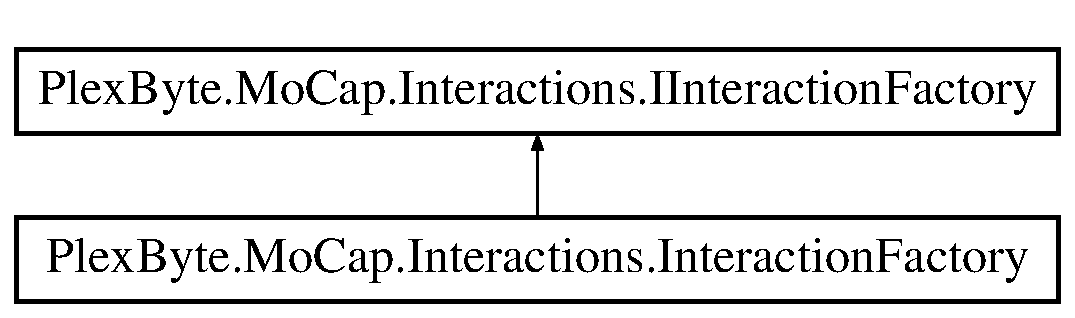
\includegraphics[height=2.000000cm]{interface_plex_byte_1_1_mo_cap_1_1_interactions_1_1_i_interaction_factory}
\end{center}
\end{figure}
\subsection*{Public Member Functions}
\begin{DoxyCompactItemize}
\item 
\hyperlink{interface_plex_byte_1_1_mo_cap_1_1_interactions_1_1_i_task}{I\+Task} \hyperlink{interface_plex_byte_1_1_mo_cap_1_1_interactions_1_1_i_interaction_factory_a2652ae146eddd246b136bfd47b55bd10}{Create\+Task} (string p\+Id, string p\+Text, I\+User p\+Creator)
\item 
\hyperlink{interface_plex_byte_1_1_mo_cap_1_1_interactions_1_1_i_task}{I\+Task} \hyperlink{interface_plex_byte_1_1_mo_cap_1_1_interactions_1_1_i_interaction_factory_ad3f030a61f41e66812ba458194a02182}{Create\+Task} (string p\+Id, string p\+Text, I\+User p\+Creator, Date\+Time p\+Start\+DT, Date\+Time p\+End\+DT, Date\+Time p\+Due\+DT)
\item 
\hyperlink{interface_plex_byte_1_1_mo_cap_1_1_interactions_1_1_i_task}{I\+Task} \hyperlink{interface_plex_byte_1_1_mo_cap_1_1_interactions_1_1_i_interaction_factory_a36f7e9ea19a2b58c4d72b7eda9568a6c}{Create\+Task} (string p\+Id, string p\+Text, string p\+Title, I\+User p\+Creator, Date\+Time p\+Start\+DT, Date\+Time p\+End\+DT, Date\+Time p\+Due\+DT, decimal p\+Budget, int p\+Duration, int p\+Priority, \hyperlink{namespace_plex_byte_1_1_mo_cap_1_1_interactions_afcb673d9186608b6bd3b187179aedc8a}{Interaction\+State} p\+State, decimal p\+Budget\+Used, int p\+Time\+Used, List$<$ \hyperlink{interface_plex_byte_1_1_mo_cap_1_1_interactions_1_1_i_task}{I\+Task} $>$ p\+Sub\+Task, int p\+Progress)
\item 
\hyperlink{interface_plex_byte_1_1_mo_cap_1_1_interactions_1_1_i_survey}{I\+Survey} \hyperlink{interface_plex_byte_1_1_mo_cap_1_1_interactions_1_1_i_interaction_factory_a10d691633579fc9ebef747595e09a1c2}{Create\+Survey} (string p\+Id, string p\+Text, List$<$ \hyperlink{interface_plex_byte_1_1_mo_cap_1_1_interactions_1_1_i_survey_option}{I\+Survey\+Option} $>$ p\+Options, I\+User p\+Creator, Date\+Time p\+Start\+DT, Date\+Time p\+End\+DT, Date\+Time p\+Due\+DT, int p\+Votes\+Per\+User, string p\+Title, \hyperlink{namespace_plex_byte_1_1_mo_cap_1_1_interactions_afcb673d9186608b6bd3b187179aedc8a}{Interaction\+State} p\+State, List$<$ \hyperlink{interface_plex_byte_1_1_mo_cap_1_1_interactions_1_1_i_vote}{I\+Vote} $>$ p\+Votes)
\item 
\hyperlink{interface_plex_byte_1_1_mo_cap_1_1_interactions_1_1_i_survey}{I\+Survey} \hyperlink{interface_plex_byte_1_1_mo_cap_1_1_interactions_1_1_i_interaction_factory_a5b5cedeba1e0748c243b7a9a5f2fb5a6}{Create\+Survey} (string p\+Id, string p\+Text, List$<$ string $>$ p\+Options, I\+User p\+Creator)
\item 
\hyperlink{interface_plex_byte_1_1_mo_cap_1_1_interactions_1_1_i_account}{I\+Account} \hyperlink{interface_plex_byte_1_1_mo_cap_1_1_interactions_1_1_i_interaction_factory_ad30e523a2735f42e372375250a1dc025}{Create\+Account} (string p\+Id, string p\+Text, I\+User p\+Creator)
\item 
\hyperlink{interface_plex_byte_1_1_mo_cap_1_1_interactions_1_1_i_account}{I\+Account} \hyperlink{interface_plex_byte_1_1_mo_cap_1_1_interactions_1_1_i_interaction_factory_a4909855456dce1184abdb5dd2d8a679d}{Create\+Account} (string p\+Id, string p\+Text, List$<$ \hyperlink{interface_plex_byte_1_1_mo_cap_1_1_interactions_1_1_i_expense}{I\+Expense} $>$ p\+Expense\+List, List$<$ \hyperlink{interface_plex_byte_1_1_mo_cap_1_1_interactions_1_1_i_timeslice}{I\+Timeslice} $>$ p\+Timeslice\+List, I\+User p\+Creator)
\item 
\hyperlink{interface_plex_byte_1_1_mo_cap_1_1_interactions_1_1_i_timeslice}{I\+Timeslice} \hyperlink{interface_plex_byte_1_1_mo_cap_1_1_interactions_1_1_i_interaction_factory_aa1e654f79711cc1d747f0e10db8c98ba}{Create\+Timeslice} (string p\+Id, I\+User p\+User, Date\+Time p\+Start\+DT, Date\+Time p\+End\+DT, \hyperlink{interface_plex_byte_1_1_mo_cap_1_1_interactions_1_1_i_interaction}{I\+Interaction} p\+Target)
\item 
\hyperlink{interface_plex_byte_1_1_mo_cap_1_1_interactions_1_1_i_timeslice}{I\+Timeslice} \hyperlink{interface_plex_byte_1_1_mo_cap_1_1_interactions_1_1_i_interaction_factory_a798b46cb4aa8a6d7bcaf47038f0150dc}{Create\+Timeslice} (string p\+Id, I\+User p\+User, int p\+Duration, \hyperlink{interface_plex_byte_1_1_mo_cap_1_1_interactions_1_1_i_interaction}{I\+Interaction} p\+Target)
\item 
\hyperlink{interface_plex_byte_1_1_mo_cap_1_1_interactions_1_1_i_expense}{I\+Expense} \hyperlink{interface_plex_byte_1_1_mo_cap_1_1_interactions_1_1_i_interaction_factory_ac85fb39c0c3072a8421e4fb3b39359cd}{Create\+Expense} (string p\+Id, string p\+Text, System.\+Drawing.\+Image p\+Receipt, decimal p\+Value, I\+User p\+User, \hyperlink{interface_plex_byte_1_1_mo_cap_1_1_interactions_1_1_i_interaction}{I\+Interaction} p\+Target)
\item 
\hyperlink{interface_plex_byte_1_1_mo_cap_1_1_interactions_1_1_i_expense}{I\+Expense} \hyperlink{interface_plex_byte_1_1_mo_cap_1_1_interactions_1_1_i_interaction_factory_a0d7c926ff7b8d7c07bdc143919f3a0f7}{Create\+Expense} (string p\+Id, string p\+Text, I\+User p\+User, \hyperlink{interface_plex_byte_1_1_mo_cap_1_1_interactions_1_1_i_interaction}{I\+Interaction} p\+Target)
\item 
\hyperlink{interface_plex_byte_1_1_mo_cap_1_1_interactions_1_1_i_project}{I\+Project} \hyperlink{interface_plex_byte_1_1_mo_cap_1_1_interactions_1_1_i_interaction_factory_a185e39ef7292fa875c3e60eead0eb1d7}{Create\+Project} (string p\+Id, string p\+Text, bool p\+Enable\+Balance, bool p\+Enable\+Survey, Date\+Time p\+Start\+DT, Date\+Time p\+End\+DT, I\+User p\+Creator)
\item 
\hyperlink{interface_plex_byte_1_1_mo_cap_1_1_interactions_1_1_i_project}{I\+Project} \hyperlink{interface_plex_byte_1_1_mo_cap_1_1_interactions_1_1_i_interaction_factory_a96f9a4cfec44b654fedcc3e62fe617ca}{Create\+Project} (string p\+Id, string p\+Text, bool p\+Enable\+Balance, bool p\+Enable\+Survey, Date\+Time p\+Start\+DT, Date\+Time p\+End\+DT, I\+User p\+Creator, I\+User p\+Owner, List$<$ I\+User $>$ \hyperlink{namespace_plex_byte_1_1_mo_cap_1_1_interactions_aa78ff2ea1c7ea92537cb6b3552b6a7daa3547319d6f4e11ac104fe2012b8c99c4}{Member\+List}, List$<$ I\+User $>$ \hyperlink{namespace_plex_byte_1_1_mo_cap_1_1_interactions_aa78ff2ea1c7ea92537cb6b3552b6a7daa1a7f5ee14da52a7231b80e347f1fe0eb}{Invitation\+List}, List$<$ \hyperlink{interface_plex_byte_1_1_mo_cap_1_1_interactions_1_1_i_task}{I\+Task} $>$ \hyperlink{namespace_plex_byte_1_1_mo_cap_1_1_interactions_aa78ff2ea1c7ea92537cb6b3552b6a7daab3f0f2eb7b25831c4e3f1d6fb7d48130}{Task\+List}, List$<$ \hyperlink{interface_plex_byte_1_1_mo_cap_1_1_interactions_1_1_i_survey}{I\+Survey} $>$ \hyperlink{namespace_plex_byte_1_1_mo_cap_1_1_interactions_aa78ff2ea1c7ea92537cb6b3552b6a7daaf698bdcd42e8985484f12fc4245a4843}{Survey\+List}, string p\+Name)
\item 
\hyperlink{interface_plex_byte_1_1_mo_cap_1_1_interactions_1_1_i_interaction}{I\+Interaction} \hyperlink{interface_plex_byte_1_1_mo_cap_1_1_interactions_1_1_i_interaction_factory_aabee33e1d8b7c8106b543dc52b218782}{Create\+Chat} (string p\+Text\+Title, I\+User p\+Creator, List$<$ I\+User $>$ p\+Users)
\item 
\hyperlink{interface_plex_byte_1_1_mo_cap_1_1_interactions_1_1_i_interaction}{I\+Interaction} \hyperlink{interface_plex_byte_1_1_mo_cap_1_1_interactions_1_1_i_interaction_factory_a41eeaa8cf6c81e669898eb2b4d57eb9b}{Create\+Chat} (string p\+Text\+Title, I\+User p\+Creator, List$<$ I\+User $>$ p\+Users, Date\+Time p\+Start\+Date\+Time, Date\+Time p\+End\+Date\+Time, bool p\+Allow\+Selfdestructing)
\item 
\hyperlink{interface_plex_byte_1_1_mo_cap_1_1_interactions_1_1_i_interaction}{I\+Interaction} \hyperlink{interface_plex_byte_1_1_mo_cap_1_1_interactions_1_1_i_interaction_factory_a7a9e3fc490901c3a0be3faadadb27494}{Create\+Interaction} (string p\+Id, Date\+Time p\+Start\+Date\+Time, Date\+Time p\+End\+Date\+Time, bool p\+Is\+Active, string p\+Text, \hyperlink{namespace_plex_byte_1_1_mo_cap_1_1_interactions_a6e7bea333446664bbce2bb296db25e31}{Interaction\+Type} p\+Type, \hyperlink{namespace_plex_byte_1_1_mo_cap_1_1_interactions_afcb673d9186608b6bd3b187179aedc8a}{Interaction\+State} p\+State, I\+User p\+Owner, I\+User p\+Creator, Date\+Time p\+Created, Date\+Time p\+Modified)
\end{DoxyCompactItemize}


\subsection{Detailed Description}


Definition at line 11 of file I\+Interaction\+Factory.\+cs.



\subsection{Member Function Documentation}
\index{Plex\+Byte\+::\+Mo\+Cap\+::\+Interactions\+::\+I\+Interaction\+Factory@{Plex\+Byte\+::\+Mo\+Cap\+::\+Interactions\+::\+I\+Interaction\+Factory}!Create\+Account@{Create\+Account}}
\index{Create\+Account@{Create\+Account}!Plex\+Byte\+::\+Mo\+Cap\+::\+Interactions\+::\+I\+Interaction\+Factory@{Plex\+Byte\+::\+Mo\+Cap\+::\+Interactions\+::\+I\+Interaction\+Factory}}
\subsubsection[{\texorpdfstring{Create\+Account(string p\+Id, string p\+Text, I\+User p\+Creator)}{CreateAccount(string pId, string pText, IUser pCreator)}}]{\setlength{\rightskip}{0pt plus 5cm}{\bf I\+Account} Plex\+Byte.\+Mo\+Cap.\+Interactions.\+I\+Interaction\+Factory.\+Create\+Account (
\begin{DoxyParamCaption}
\item[{string}]{p\+Id, }
\item[{string}]{p\+Text, }
\item[{I\+User}]{p\+Creator}
\end{DoxyParamCaption}
)}\hypertarget{interface_plex_byte_1_1_mo_cap_1_1_interactions_1_1_i_interaction_factory_ad30e523a2735f42e372375250a1dc025}{}\label{interface_plex_byte_1_1_mo_cap_1_1_interactions_1_1_i_interaction_factory_ad30e523a2735f42e372375250a1dc025}


Implemented in \hyperlink{class_plex_byte_1_1_mo_cap_1_1_interactions_1_1_interaction_factory_a08413bc140420733e410b17c2262e7ee}{Plex\+Byte.\+Mo\+Cap.\+Interactions.\+Interaction\+Factory}.

\index{Plex\+Byte\+::\+Mo\+Cap\+::\+Interactions\+::\+I\+Interaction\+Factory@{Plex\+Byte\+::\+Mo\+Cap\+::\+Interactions\+::\+I\+Interaction\+Factory}!Create\+Account@{Create\+Account}}
\index{Create\+Account@{Create\+Account}!Plex\+Byte\+::\+Mo\+Cap\+::\+Interactions\+::\+I\+Interaction\+Factory@{Plex\+Byte\+::\+Mo\+Cap\+::\+Interactions\+::\+I\+Interaction\+Factory}}
\subsubsection[{\texorpdfstring{Create\+Account(string p\+Id, string p\+Text, List$<$ I\+Expense $>$ p\+Expense\+List, List$<$ I\+Timeslice $>$ p\+Timeslice\+List, I\+User p\+Creator)}{CreateAccount(string pId, string pText, List< IExpense > pExpenseList, List< ITimeslice > pTimesliceList, IUser pCreator)}}]{\setlength{\rightskip}{0pt plus 5cm}{\bf I\+Account} Plex\+Byte.\+Mo\+Cap.\+Interactions.\+I\+Interaction\+Factory.\+Create\+Account (
\begin{DoxyParamCaption}
\item[{string}]{p\+Id, }
\item[{string}]{p\+Text, }
\item[{List$<$ {\bf I\+Expense} $>$}]{p\+Expense\+List, }
\item[{List$<$ {\bf I\+Timeslice} $>$}]{p\+Timeslice\+List, }
\item[{I\+User}]{p\+Creator}
\end{DoxyParamCaption}
)}\hypertarget{interface_plex_byte_1_1_mo_cap_1_1_interactions_1_1_i_interaction_factory_a4909855456dce1184abdb5dd2d8a679d}{}\label{interface_plex_byte_1_1_mo_cap_1_1_interactions_1_1_i_interaction_factory_a4909855456dce1184abdb5dd2d8a679d}


Implemented in \hyperlink{class_plex_byte_1_1_mo_cap_1_1_interactions_1_1_interaction_factory_a1d79c272ff2a70b71f7c8188756a0ae8}{Plex\+Byte.\+Mo\+Cap.\+Interactions.\+Interaction\+Factory}.

\index{Plex\+Byte\+::\+Mo\+Cap\+::\+Interactions\+::\+I\+Interaction\+Factory@{Plex\+Byte\+::\+Mo\+Cap\+::\+Interactions\+::\+I\+Interaction\+Factory}!Create\+Chat@{Create\+Chat}}
\index{Create\+Chat@{Create\+Chat}!Plex\+Byte\+::\+Mo\+Cap\+::\+Interactions\+::\+I\+Interaction\+Factory@{Plex\+Byte\+::\+Mo\+Cap\+::\+Interactions\+::\+I\+Interaction\+Factory}}
\subsubsection[{\texorpdfstring{Create\+Chat(string p\+Text\+Title, I\+User p\+Creator, List$<$ I\+User $>$ p\+Users)}{CreateChat(string pTextTitle, IUser pCreator, List< IUser > pUsers)}}]{\setlength{\rightskip}{0pt plus 5cm}{\bf I\+Interaction} Plex\+Byte.\+Mo\+Cap.\+Interactions.\+I\+Interaction\+Factory.\+Create\+Chat (
\begin{DoxyParamCaption}
\item[{string}]{p\+Text\+Title, }
\item[{I\+User}]{p\+Creator, }
\item[{List$<$ I\+User $>$}]{p\+Users}
\end{DoxyParamCaption}
)}\hypertarget{interface_plex_byte_1_1_mo_cap_1_1_interactions_1_1_i_interaction_factory_aabee33e1d8b7c8106b543dc52b218782}{}\label{interface_plex_byte_1_1_mo_cap_1_1_interactions_1_1_i_interaction_factory_aabee33e1d8b7c8106b543dc52b218782}


Implemented in \hyperlink{class_plex_byte_1_1_mo_cap_1_1_interactions_1_1_interaction_factory_a8499cf461c2028c8e47f61056856a47d}{Plex\+Byte.\+Mo\+Cap.\+Interactions.\+Interaction\+Factory}.

\index{Plex\+Byte\+::\+Mo\+Cap\+::\+Interactions\+::\+I\+Interaction\+Factory@{Plex\+Byte\+::\+Mo\+Cap\+::\+Interactions\+::\+I\+Interaction\+Factory}!Create\+Chat@{Create\+Chat}}
\index{Create\+Chat@{Create\+Chat}!Plex\+Byte\+::\+Mo\+Cap\+::\+Interactions\+::\+I\+Interaction\+Factory@{Plex\+Byte\+::\+Mo\+Cap\+::\+Interactions\+::\+I\+Interaction\+Factory}}
\subsubsection[{\texorpdfstring{Create\+Chat(string p\+Text\+Title, I\+User p\+Creator, List$<$ I\+User $>$ p\+Users, Date\+Time p\+Start\+Date\+Time, Date\+Time p\+End\+Date\+Time, bool p\+Allow\+Selfdestructing)}{CreateChat(string pTextTitle, IUser pCreator, List< IUser > pUsers, DateTime pStartDateTime, DateTime pEndDateTime, bool pAllowSelfdestructing)}}]{\setlength{\rightskip}{0pt plus 5cm}{\bf I\+Interaction} Plex\+Byte.\+Mo\+Cap.\+Interactions.\+I\+Interaction\+Factory.\+Create\+Chat (
\begin{DoxyParamCaption}
\item[{string}]{p\+Text\+Title, }
\item[{I\+User}]{p\+Creator, }
\item[{List$<$ I\+User $>$}]{p\+Users, }
\item[{Date\+Time}]{p\+Start\+Date\+Time, }
\item[{Date\+Time}]{p\+End\+Date\+Time, }
\item[{bool}]{p\+Allow\+Selfdestructing}
\end{DoxyParamCaption}
)}\hypertarget{interface_plex_byte_1_1_mo_cap_1_1_interactions_1_1_i_interaction_factory_a41eeaa8cf6c81e669898eb2b4d57eb9b}{}\label{interface_plex_byte_1_1_mo_cap_1_1_interactions_1_1_i_interaction_factory_a41eeaa8cf6c81e669898eb2b4d57eb9b}


Implemented in \hyperlink{class_plex_byte_1_1_mo_cap_1_1_interactions_1_1_interaction_factory_a90e50fa9b778353e619c059ea5b78822}{Plex\+Byte.\+Mo\+Cap.\+Interactions.\+Interaction\+Factory}.

\index{Plex\+Byte\+::\+Mo\+Cap\+::\+Interactions\+::\+I\+Interaction\+Factory@{Plex\+Byte\+::\+Mo\+Cap\+::\+Interactions\+::\+I\+Interaction\+Factory}!Create\+Expense@{Create\+Expense}}
\index{Create\+Expense@{Create\+Expense}!Plex\+Byte\+::\+Mo\+Cap\+::\+Interactions\+::\+I\+Interaction\+Factory@{Plex\+Byte\+::\+Mo\+Cap\+::\+Interactions\+::\+I\+Interaction\+Factory}}
\subsubsection[{\texorpdfstring{Create\+Expense(string p\+Id, string p\+Text, System.\+Drawing.\+Image p\+Receipt, decimal p\+Value, I\+User p\+User, I\+Interaction p\+Target)}{CreateExpense(string pId, string pText, System.Drawing.Image pReceipt, decimal pValue, IUser pUser, IInteraction pTarget)}}]{\setlength{\rightskip}{0pt plus 5cm}{\bf I\+Expense} Plex\+Byte.\+Mo\+Cap.\+Interactions.\+I\+Interaction\+Factory.\+Create\+Expense (
\begin{DoxyParamCaption}
\item[{string}]{p\+Id, }
\item[{string}]{p\+Text, }
\item[{System.\+Drawing.\+Image}]{p\+Receipt, }
\item[{decimal}]{p\+Value, }
\item[{I\+User}]{p\+User, }
\item[{{\bf I\+Interaction}}]{p\+Target}
\end{DoxyParamCaption}
)}\hypertarget{interface_plex_byte_1_1_mo_cap_1_1_interactions_1_1_i_interaction_factory_ac85fb39c0c3072a8421e4fb3b39359cd}{}\label{interface_plex_byte_1_1_mo_cap_1_1_interactions_1_1_i_interaction_factory_ac85fb39c0c3072a8421e4fb3b39359cd}


Implemented in \hyperlink{class_plex_byte_1_1_mo_cap_1_1_interactions_1_1_interaction_factory_a6d6a4839a754494e5db0adbb69fccc94}{Plex\+Byte.\+Mo\+Cap.\+Interactions.\+Interaction\+Factory}.

\index{Plex\+Byte\+::\+Mo\+Cap\+::\+Interactions\+::\+I\+Interaction\+Factory@{Plex\+Byte\+::\+Mo\+Cap\+::\+Interactions\+::\+I\+Interaction\+Factory}!Create\+Expense@{Create\+Expense}}
\index{Create\+Expense@{Create\+Expense}!Plex\+Byte\+::\+Mo\+Cap\+::\+Interactions\+::\+I\+Interaction\+Factory@{Plex\+Byte\+::\+Mo\+Cap\+::\+Interactions\+::\+I\+Interaction\+Factory}}
\subsubsection[{\texorpdfstring{Create\+Expense(string p\+Id, string p\+Text, I\+User p\+User, I\+Interaction p\+Target)}{CreateExpense(string pId, string pText, IUser pUser, IInteraction pTarget)}}]{\setlength{\rightskip}{0pt plus 5cm}{\bf I\+Expense} Plex\+Byte.\+Mo\+Cap.\+Interactions.\+I\+Interaction\+Factory.\+Create\+Expense (
\begin{DoxyParamCaption}
\item[{string}]{p\+Id, }
\item[{string}]{p\+Text, }
\item[{I\+User}]{p\+User, }
\item[{{\bf I\+Interaction}}]{p\+Target}
\end{DoxyParamCaption}
)}\hypertarget{interface_plex_byte_1_1_mo_cap_1_1_interactions_1_1_i_interaction_factory_a0d7c926ff7b8d7c07bdc143919f3a0f7}{}\label{interface_plex_byte_1_1_mo_cap_1_1_interactions_1_1_i_interaction_factory_a0d7c926ff7b8d7c07bdc143919f3a0f7}


Implemented in \hyperlink{class_plex_byte_1_1_mo_cap_1_1_interactions_1_1_interaction_factory_a40751419f32c51ae9cfa556b22c8fd7f}{Plex\+Byte.\+Mo\+Cap.\+Interactions.\+Interaction\+Factory}.

\index{Plex\+Byte\+::\+Mo\+Cap\+::\+Interactions\+::\+I\+Interaction\+Factory@{Plex\+Byte\+::\+Mo\+Cap\+::\+Interactions\+::\+I\+Interaction\+Factory}!Create\+Interaction@{Create\+Interaction}}
\index{Create\+Interaction@{Create\+Interaction}!Plex\+Byte\+::\+Mo\+Cap\+::\+Interactions\+::\+I\+Interaction\+Factory@{Plex\+Byte\+::\+Mo\+Cap\+::\+Interactions\+::\+I\+Interaction\+Factory}}
\subsubsection[{\texorpdfstring{Create\+Interaction(string p\+Id, Date\+Time p\+Start\+Date\+Time, Date\+Time p\+End\+Date\+Time, bool p\+Is\+Active, string p\+Text, Interaction\+Type p\+Type, Interaction\+State p\+State, I\+User p\+Owner, I\+User p\+Creator, Date\+Time p\+Created, Date\+Time p\+Modified)}{CreateInteraction(string pId, DateTime pStartDateTime, DateTime pEndDateTime, bool pIsActive, string pText, InteractionType pType, InteractionState pState, IUser pOwner, IUser pCreator, DateTime pCreated, DateTime pModified)}}]{\setlength{\rightskip}{0pt plus 5cm}{\bf I\+Interaction} Plex\+Byte.\+Mo\+Cap.\+Interactions.\+I\+Interaction\+Factory.\+Create\+Interaction (
\begin{DoxyParamCaption}
\item[{string}]{p\+Id, }
\item[{Date\+Time}]{p\+Start\+Date\+Time, }
\item[{Date\+Time}]{p\+End\+Date\+Time, }
\item[{bool}]{p\+Is\+Active, }
\item[{string}]{p\+Text, }
\item[{{\bf Interaction\+Type}}]{p\+Type, }
\item[{{\bf Interaction\+State}}]{p\+State, }
\item[{I\+User}]{p\+Owner, }
\item[{I\+User}]{p\+Creator, }
\item[{Date\+Time}]{p\+Created, }
\item[{Date\+Time}]{p\+Modified}
\end{DoxyParamCaption}
)}\hypertarget{interface_plex_byte_1_1_mo_cap_1_1_interactions_1_1_i_interaction_factory_a7a9e3fc490901c3a0be3faadadb27494}{}\label{interface_plex_byte_1_1_mo_cap_1_1_interactions_1_1_i_interaction_factory_a7a9e3fc490901c3a0be3faadadb27494}


Implemented in \hyperlink{class_plex_byte_1_1_mo_cap_1_1_interactions_1_1_interaction_factory_a43297682c502977cf7ebc69a9fe8b15f}{Plex\+Byte.\+Mo\+Cap.\+Interactions.\+Interaction\+Factory}.

\index{Plex\+Byte\+::\+Mo\+Cap\+::\+Interactions\+::\+I\+Interaction\+Factory@{Plex\+Byte\+::\+Mo\+Cap\+::\+Interactions\+::\+I\+Interaction\+Factory}!Create\+Project@{Create\+Project}}
\index{Create\+Project@{Create\+Project}!Plex\+Byte\+::\+Mo\+Cap\+::\+Interactions\+::\+I\+Interaction\+Factory@{Plex\+Byte\+::\+Mo\+Cap\+::\+Interactions\+::\+I\+Interaction\+Factory}}
\subsubsection[{\texorpdfstring{Create\+Project(string p\+Id, string p\+Text, bool p\+Enable\+Balance, bool p\+Enable\+Survey, Date\+Time p\+Start\+D\+T, Date\+Time p\+End\+D\+T, I\+User p\+Creator)}{CreateProject(string pId, string pText, bool pEnableBalance, bool pEnableSurvey, DateTime pStartDT, DateTime pEndDT, IUser pCreator)}}]{\setlength{\rightskip}{0pt plus 5cm}{\bf I\+Project} Plex\+Byte.\+Mo\+Cap.\+Interactions.\+I\+Interaction\+Factory.\+Create\+Project (
\begin{DoxyParamCaption}
\item[{string}]{p\+Id, }
\item[{string}]{p\+Text, }
\item[{bool}]{p\+Enable\+Balance, }
\item[{bool}]{p\+Enable\+Survey, }
\item[{Date\+Time}]{p\+Start\+DT, }
\item[{Date\+Time}]{p\+End\+DT, }
\item[{I\+User}]{p\+Creator}
\end{DoxyParamCaption}
)}\hypertarget{interface_plex_byte_1_1_mo_cap_1_1_interactions_1_1_i_interaction_factory_a185e39ef7292fa875c3e60eead0eb1d7}{}\label{interface_plex_byte_1_1_mo_cap_1_1_interactions_1_1_i_interaction_factory_a185e39ef7292fa875c3e60eead0eb1d7}


Implemented in \hyperlink{class_plex_byte_1_1_mo_cap_1_1_interactions_1_1_interaction_factory_a38a010ef1a5e042ccbb1250adaa2324d}{Plex\+Byte.\+Mo\+Cap.\+Interactions.\+Interaction\+Factory}.

\index{Plex\+Byte\+::\+Mo\+Cap\+::\+Interactions\+::\+I\+Interaction\+Factory@{Plex\+Byte\+::\+Mo\+Cap\+::\+Interactions\+::\+I\+Interaction\+Factory}!Create\+Project@{Create\+Project}}
\index{Create\+Project@{Create\+Project}!Plex\+Byte\+::\+Mo\+Cap\+::\+Interactions\+::\+I\+Interaction\+Factory@{Plex\+Byte\+::\+Mo\+Cap\+::\+Interactions\+::\+I\+Interaction\+Factory}}
\subsubsection[{\texorpdfstring{Create\+Project(string p\+Id, string p\+Text, bool p\+Enable\+Balance, bool p\+Enable\+Survey, Date\+Time p\+Start\+D\+T, Date\+Time p\+End\+D\+T, I\+User p\+Creator, I\+User p\+Owner, List$<$ I\+User $>$ Member\+List, List$<$ I\+User $>$ Invitation\+List, List$<$ I\+Task $>$ Task\+List, List$<$ I\+Survey $>$ Survey\+List, string p\+Name)}{CreateProject(string pId, string pText, bool pEnableBalance, bool pEnableSurvey, DateTime pStartDT, DateTime pEndDT, IUser pCreator, IUser pOwner, List< IUser > MemberList, List< IUser > InvitationList, List< ITask > TaskList, List< ISurvey > SurveyList, string pName)}}]{\setlength{\rightskip}{0pt plus 5cm}{\bf I\+Project} Plex\+Byte.\+Mo\+Cap.\+Interactions.\+I\+Interaction\+Factory.\+Create\+Project (
\begin{DoxyParamCaption}
\item[{string}]{p\+Id, }
\item[{string}]{p\+Text, }
\item[{bool}]{p\+Enable\+Balance, }
\item[{bool}]{p\+Enable\+Survey, }
\item[{Date\+Time}]{p\+Start\+DT, }
\item[{Date\+Time}]{p\+End\+DT, }
\item[{I\+User}]{p\+Creator, }
\item[{I\+User}]{p\+Owner, }
\item[{List$<$ I\+User $>$}]{Member\+List, }
\item[{List$<$ I\+User $>$}]{Invitation\+List, }
\item[{List$<$ {\bf I\+Task} $>$}]{Task\+List, }
\item[{List$<$ {\bf I\+Survey} $>$}]{Survey\+List, }
\item[{string}]{p\+Name}
\end{DoxyParamCaption}
)}\hypertarget{interface_plex_byte_1_1_mo_cap_1_1_interactions_1_1_i_interaction_factory_a96f9a4cfec44b654fedcc3e62fe617ca}{}\label{interface_plex_byte_1_1_mo_cap_1_1_interactions_1_1_i_interaction_factory_a96f9a4cfec44b654fedcc3e62fe617ca}


Implemented in \hyperlink{class_plex_byte_1_1_mo_cap_1_1_interactions_1_1_interaction_factory_ab8dddf10ff7dd5720603c1859d96a78d}{Plex\+Byte.\+Mo\+Cap.\+Interactions.\+Interaction\+Factory}.

\index{Plex\+Byte\+::\+Mo\+Cap\+::\+Interactions\+::\+I\+Interaction\+Factory@{Plex\+Byte\+::\+Mo\+Cap\+::\+Interactions\+::\+I\+Interaction\+Factory}!Create\+Survey@{Create\+Survey}}
\index{Create\+Survey@{Create\+Survey}!Plex\+Byte\+::\+Mo\+Cap\+::\+Interactions\+::\+I\+Interaction\+Factory@{Plex\+Byte\+::\+Mo\+Cap\+::\+Interactions\+::\+I\+Interaction\+Factory}}
\subsubsection[{\texorpdfstring{Create\+Survey(string p\+Id, string p\+Text, List$<$ I\+Survey\+Option $>$ p\+Options, I\+User p\+Creator, Date\+Time p\+Start\+D\+T, Date\+Time p\+End\+D\+T, Date\+Time p\+Due\+D\+T, int p\+Votes\+Per\+User, string p\+Title, Interaction\+State p\+State, List$<$ I\+Vote $>$ p\+Votes)}{CreateSurvey(string pId, string pText, List< ISurveyOption > pOptions, IUser pCreator, DateTime pStartDT, DateTime pEndDT, DateTime pDueDT, int pVotesPerUser, string pTitle, InteractionState pState, List< IVote > pVotes)}}]{\setlength{\rightskip}{0pt plus 5cm}{\bf I\+Survey} Plex\+Byte.\+Mo\+Cap.\+Interactions.\+I\+Interaction\+Factory.\+Create\+Survey (
\begin{DoxyParamCaption}
\item[{string}]{p\+Id, }
\item[{string}]{p\+Text, }
\item[{List$<$ {\bf I\+Survey\+Option} $>$}]{p\+Options, }
\item[{I\+User}]{p\+Creator, }
\item[{Date\+Time}]{p\+Start\+DT, }
\item[{Date\+Time}]{p\+End\+DT, }
\item[{Date\+Time}]{p\+Due\+DT, }
\item[{int}]{p\+Votes\+Per\+User, }
\item[{string}]{p\+Title, }
\item[{{\bf Interaction\+State}}]{p\+State, }
\item[{List$<$ {\bf I\+Vote} $>$}]{p\+Votes}
\end{DoxyParamCaption}
)}\hypertarget{interface_plex_byte_1_1_mo_cap_1_1_interactions_1_1_i_interaction_factory_a10d691633579fc9ebef747595e09a1c2}{}\label{interface_plex_byte_1_1_mo_cap_1_1_interactions_1_1_i_interaction_factory_a10d691633579fc9ebef747595e09a1c2}


Implemented in \hyperlink{class_plex_byte_1_1_mo_cap_1_1_interactions_1_1_interaction_factory_a91bccc9e26b2a3ebdf9210f88e12777f}{Plex\+Byte.\+Mo\+Cap.\+Interactions.\+Interaction\+Factory}.

\index{Plex\+Byte\+::\+Mo\+Cap\+::\+Interactions\+::\+I\+Interaction\+Factory@{Plex\+Byte\+::\+Mo\+Cap\+::\+Interactions\+::\+I\+Interaction\+Factory}!Create\+Survey@{Create\+Survey}}
\index{Create\+Survey@{Create\+Survey}!Plex\+Byte\+::\+Mo\+Cap\+::\+Interactions\+::\+I\+Interaction\+Factory@{Plex\+Byte\+::\+Mo\+Cap\+::\+Interactions\+::\+I\+Interaction\+Factory}}
\subsubsection[{\texorpdfstring{Create\+Survey(string p\+Id, string p\+Text, List$<$ string $>$ p\+Options, I\+User p\+Creator)}{CreateSurvey(string pId, string pText, List< string > pOptions, IUser pCreator)}}]{\setlength{\rightskip}{0pt plus 5cm}{\bf I\+Survey} Plex\+Byte.\+Mo\+Cap.\+Interactions.\+I\+Interaction\+Factory.\+Create\+Survey (
\begin{DoxyParamCaption}
\item[{string}]{p\+Id, }
\item[{string}]{p\+Text, }
\item[{List$<$ string $>$}]{p\+Options, }
\item[{I\+User}]{p\+Creator}
\end{DoxyParamCaption}
)}\hypertarget{interface_plex_byte_1_1_mo_cap_1_1_interactions_1_1_i_interaction_factory_a5b5cedeba1e0748c243b7a9a5f2fb5a6}{}\label{interface_plex_byte_1_1_mo_cap_1_1_interactions_1_1_i_interaction_factory_a5b5cedeba1e0748c243b7a9a5f2fb5a6}


Implemented in \hyperlink{class_plex_byte_1_1_mo_cap_1_1_interactions_1_1_interaction_factory_a7cca7832aa0ee7ac17fa5f0339eeed2c}{Plex\+Byte.\+Mo\+Cap.\+Interactions.\+Interaction\+Factory}.

\index{Plex\+Byte\+::\+Mo\+Cap\+::\+Interactions\+::\+I\+Interaction\+Factory@{Plex\+Byte\+::\+Mo\+Cap\+::\+Interactions\+::\+I\+Interaction\+Factory}!Create\+Task@{Create\+Task}}
\index{Create\+Task@{Create\+Task}!Plex\+Byte\+::\+Mo\+Cap\+::\+Interactions\+::\+I\+Interaction\+Factory@{Plex\+Byte\+::\+Mo\+Cap\+::\+Interactions\+::\+I\+Interaction\+Factory}}
\subsubsection[{\texorpdfstring{Create\+Task(string p\+Id, string p\+Text, I\+User p\+Creator)}{CreateTask(string pId, string pText, IUser pCreator)}}]{\setlength{\rightskip}{0pt plus 5cm}{\bf I\+Task} Plex\+Byte.\+Mo\+Cap.\+Interactions.\+I\+Interaction\+Factory.\+Create\+Task (
\begin{DoxyParamCaption}
\item[{string}]{p\+Id, }
\item[{string}]{p\+Text, }
\item[{I\+User}]{p\+Creator}
\end{DoxyParamCaption}
)}\hypertarget{interface_plex_byte_1_1_mo_cap_1_1_interactions_1_1_i_interaction_factory_a2652ae146eddd246b136bfd47b55bd10}{}\label{interface_plex_byte_1_1_mo_cap_1_1_interactions_1_1_i_interaction_factory_a2652ae146eddd246b136bfd47b55bd10}


Implemented in \hyperlink{class_plex_byte_1_1_mo_cap_1_1_interactions_1_1_interaction_factory_a9a7f2eed60a838269aa2a4444e50ecef}{Plex\+Byte.\+Mo\+Cap.\+Interactions.\+Interaction\+Factory}.

\index{Plex\+Byte\+::\+Mo\+Cap\+::\+Interactions\+::\+I\+Interaction\+Factory@{Plex\+Byte\+::\+Mo\+Cap\+::\+Interactions\+::\+I\+Interaction\+Factory}!Create\+Task@{Create\+Task}}
\index{Create\+Task@{Create\+Task}!Plex\+Byte\+::\+Mo\+Cap\+::\+Interactions\+::\+I\+Interaction\+Factory@{Plex\+Byte\+::\+Mo\+Cap\+::\+Interactions\+::\+I\+Interaction\+Factory}}
\subsubsection[{\texorpdfstring{Create\+Task(string p\+Id, string p\+Text, I\+User p\+Creator, Date\+Time p\+Start\+D\+T, Date\+Time p\+End\+D\+T, Date\+Time p\+Due\+D\+T)}{CreateTask(string pId, string pText, IUser pCreator, DateTime pStartDT, DateTime pEndDT, DateTime pDueDT)}}]{\setlength{\rightskip}{0pt plus 5cm}{\bf I\+Task} Plex\+Byte.\+Mo\+Cap.\+Interactions.\+I\+Interaction\+Factory.\+Create\+Task (
\begin{DoxyParamCaption}
\item[{string}]{p\+Id, }
\item[{string}]{p\+Text, }
\item[{I\+User}]{p\+Creator, }
\item[{Date\+Time}]{p\+Start\+DT, }
\item[{Date\+Time}]{p\+End\+DT, }
\item[{Date\+Time}]{p\+Due\+DT}
\end{DoxyParamCaption}
)}\hypertarget{interface_plex_byte_1_1_mo_cap_1_1_interactions_1_1_i_interaction_factory_ad3f030a61f41e66812ba458194a02182}{}\label{interface_plex_byte_1_1_mo_cap_1_1_interactions_1_1_i_interaction_factory_ad3f030a61f41e66812ba458194a02182}


Implemented in \hyperlink{class_plex_byte_1_1_mo_cap_1_1_interactions_1_1_interaction_factory_ab49d25714033edffd3bd5c87e453a237}{Plex\+Byte.\+Mo\+Cap.\+Interactions.\+Interaction\+Factory}.

\index{Plex\+Byte\+::\+Mo\+Cap\+::\+Interactions\+::\+I\+Interaction\+Factory@{Plex\+Byte\+::\+Mo\+Cap\+::\+Interactions\+::\+I\+Interaction\+Factory}!Create\+Task@{Create\+Task}}
\index{Create\+Task@{Create\+Task}!Plex\+Byte\+::\+Mo\+Cap\+::\+Interactions\+::\+I\+Interaction\+Factory@{Plex\+Byte\+::\+Mo\+Cap\+::\+Interactions\+::\+I\+Interaction\+Factory}}
\subsubsection[{\texorpdfstring{Create\+Task(string p\+Id, string p\+Text, string p\+Title, I\+User p\+Creator, Date\+Time p\+Start\+D\+T, Date\+Time p\+End\+D\+T, Date\+Time p\+Due\+D\+T, decimal p\+Budget, int p\+Duration, int p\+Priority, Interaction\+State p\+State, decimal p\+Budget\+Used, int p\+Time\+Used, List$<$ I\+Task $>$ p\+Sub\+Task, int p\+Progress)}{CreateTask(string pId, string pText, string pTitle, IUser pCreator, DateTime pStartDT, DateTime pEndDT, DateTime pDueDT, decimal pBudget, int pDuration, int pPriority, InteractionState pState, decimal pBudgetUsed, int pTimeUsed, List< ITask > pSubTask, int pProgress)}}]{\setlength{\rightskip}{0pt plus 5cm}{\bf I\+Task} Plex\+Byte.\+Mo\+Cap.\+Interactions.\+I\+Interaction\+Factory.\+Create\+Task (
\begin{DoxyParamCaption}
\item[{string}]{p\+Id, }
\item[{string}]{p\+Text, }
\item[{string}]{p\+Title, }
\item[{I\+User}]{p\+Creator, }
\item[{Date\+Time}]{p\+Start\+DT, }
\item[{Date\+Time}]{p\+End\+DT, }
\item[{Date\+Time}]{p\+Due\+DT, }
\item[{decimal}]{p\+Budget, }
\item[{int}]{p\+Duration, }
\item[{int}]{p\+Priority, }
\item[{{\bf Interaction\+State}}]{p\+State, }
\item[{decimal}]{p\+Budget\+Used, }
\item[{int}]{p\+Time\+Used, }
\item[{List$<$ {\bf I\+Task} $>$}]{p\+Sub\+Task, }
\item[{int}]{p\+Progress}
\end{DoxyParamCaption}
)}\hypertarget{interface_plex_byte_1_1_mo_cap_1_1_interactions_1_1_i_interaction_factory_a36f7e9ea19a2b58c4d72b7eda9568a6c}{}\label{interface_plex_byte_1_1_mo_cap_1_1_interactions_1_1_i_interaction_factory_a36f7e9ea19a2b58c4d72b7eda9568a6c}


Implemented in \hyperlink{class_plex_byte_1_1_mo_cap_1_1_interactions_1_1_interaction_factory_a030a74854486e68be1cb97166214ef16}{Plex\+Byte.\+Mo\+Cap.\+Interactions.\+Interaction\+Factory}.

\index{Plex\+Byte\+::\+Mo\+Cap\+::\+Interactions\+::\+I\+Interaction\+Factory@{Plex\+Byte\+::\+Mo\+Cap\+::\+Interactions\+::\+I\+Interaction\+Factory}!Create\+Timeslice@{Create\+Timeslice}}
\index{Create\+Timeslice@{Create\+Timeslice}!Plex\+Byte\+::\+Mo\+Cap\+::\+Interactions\+::\+I\+Interaction\+Factory@{Plex\+Byte\+::\+Mo\+Cap\+::\+Interactions\+::\+I\+Interaction\+Factory}}
\subsubsection[{\texorpdfstring{Create\+Timeslice(string p\+Id, I\+User p\+User, Date\+Time p\+Start\+D\+T, Date\+Time p\+End\+D\+T, I\+Interaction p\+Target)}{CreateTimeslice(string pId, IUser pUser, DateTime pStartDT, DateTime pEndDT, IInteraction pTarget)}}]{\setlength{\rightskip}{0pt plus 5cm}{\bf I\+Timeslice} Plex\+Byte.\+Mo\+Cap.\+Interactions.\+I\+Interaction\+Factory.\+Create\+Timeslice (
\begin{DoxyParamCaption}
\item[{string}]{p\+Id, }
\item[{I\+User}]{p\+User, }
\item[{Date\+Time}]{p\+Start\+DT, }
\item[{Date\+Time}]{p\+End\+DT, }
\item[{{\bf I\+Interaction}}]{p\+Target}
\end{DoxyParamCaption}
)}\hypertarget{interface_plex_byte_1_1_mo_cap_1_1_interactions_1_1_i_interaction_factory_aa1e654f79711cc1d747f0e10db8c98ba}{}\label{interface_plex_byte_1_1_mo_cap_1_1_interactions_1_1_i_interaction_factory_aa1e654f79711cc1d747f0e10db8c98ba}


Implemented in \hyperlink{class_plex_byte_1_1_mo_cap_1_1_interactions_1_1_interaction_factory_a09b8c47419a3eefd5823056f72c47130}{Plex\+Byte.\+Mo\+Cap.\+Interactions.\+Interaction\+Factory}.

\index{Plex\+Byte\+::\+Mo\+Cap\+::\+Interactions\+::\+I\+Interaction\+Factory@{Plex\+Byte\+::\+Mo\+Cap\+::\+Interactions\+::\+I\+Interaction\+Factory}!Create\+Timeslice@{Create\+Timeslice}}
\index{Create\+Timeslice@{Create\+Timeslice}!Plex\+Byte\+::\+Mo\+Cap\+::\+Interactions\+::\+I\+Interaction\+Factory@{Plex\+Byte\+::\+Mo\+Cap\+::\+Interactions\+::\+I\+Interaction\+Factory}}
\subsubsection[{\texorpdfstring{Create\+Timeslice(string p\+Id, I\+User p\+User, int p\+Duration, I\+Interaction p\+Target)}{CreateTimeslice(string pId, IUser pUser, int pDuration, IInteraction pTarget)}}]{\setlength{\rightskip}{0pt plus 5cm}{\bf I\+Timeslice} Plex\+Byte.\+Mo\+Cap.\+Interactions.\+I\+Interaction\+Factory.\+Create\+Timeslice (
\begin{DoxyParamCaption}
\item[{string}]{p\+Id, }
\item[{I\+User}]{p\+User, }
\item[{int}]{p\+Duration, }
\item[{{\bf I\+Interaction}}]{p\+Target}
\end{DoxyParamCaption}
)}\hypertarget{interface_plex_byte_1_1_mo_cap_1_1_interactions_1_1_i_interaction_factory_a798b46cb4aa8a6d7bcaf47038f0150dc}{}\label{interface_plex_byte_1_1_mo_cap_1_1_interactions_1_1_i_interaction_factory_a798b46cb4aa8a6d7bcaf47038f0150dc}


Implemented in \hyperlink{class_plex_byte_1_1_mo_cap_1_1_interactions_1_1_interaction_factory_a66108b416dc8f455fd0dc22123b2d143}{Plex\+Byte.\+Mo\+Cap.\+Interactions.\+Interaction\+Factory}.



The documentation for this interface was generated from the following file\+:\begin{DoxyCompactItemize}
\item 
D\+:/\+Users/\+Christian\+B/\+Documents/\+\_\+\+H\+F Infomatik/\+Git\+Hub\+\_\+\+Repos/\+Mo\+Cap/\+Plex\+Byte.\+Mo\+Cap/\+Plex\+Byte.\+Mo\+Cap.\+Interactions/\hyperlink{_i_interaction_factory_8cs}{I\+Interaction\+Factory.\+cs}\end{DoxyCompactItemize}

\hypertarget{class_plex_byte_1_1_mo_cap_1_1_interactions_1_1_interaction}{}\section{Plex\+Byte.\+Mo\+Cap.\+Interactions.\+Interaction Class Reference}
\label{class_plex_byte_1_1_mo_cap_1_1_interactions_1_1_interaction}\index{Plex\+Byte.\+Mo\+Cap.\+Interactions.\+Interaction@{Plex\+Byte.\+Mo\+Cap.\+Interactions.\+Interaction}}
Inheritance diagram for Plex\+Byte.\+Mo\+Cap.\+Interactions.\+Interaction\+:\begin{figure}[H]
\begin{center}
\leavevmode
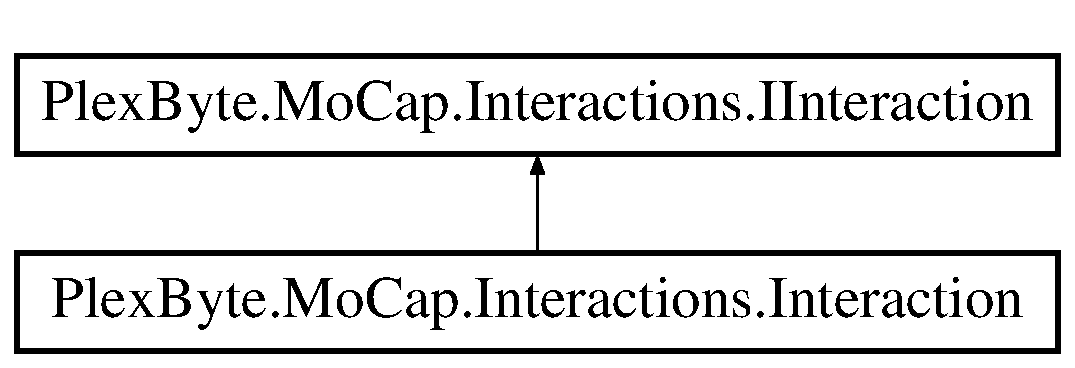
\includegraphics[height=2.000000cm]{class_plex_byte_1_1_mo_cap_1_1_interactions_1_1_interaction}
\end{center}
\end{figure}
\subsection*{Public Member Functions}
\begin{DoxyCompactItemize}
\item 
void \hyperlink{class_plex_byte_1_1_mo_cap_1_1_interactions_1_1_interaction_a0a837bb8d58f8e2077ba901fadd650a6}{On\+Complete} (\hyperlink{class_plex_byte_1_1_mo_cap_1_1_interactions_1_1_interaction_event_args}{Interaction\+Event\+Args} p\+Event\+Args)
\item 
void \hyperlink{class_plex_byte_1_1_mo_cap_1_1_interactions_1_1_interaction_a4ef64eb1f5bb5e03d1d5ef5cec52f759}{Change\+Owner} (I\+User p\+User)
\item 
void \hyperlink{class_plex_byte_1_1_mo_cap_1_1_interactions_1_1_interaction_ab58345952cc115beaa62f8e556387b87}{Change\+Is\+Active} (bool p\+Active)
\item 
void \hyperlink{class_plex_byte_1_1_mo_cap_1_1_interactions_1_1_interaction_a2f011b1cd2c0e01d8caca6f57c60deec}{On\+Modify} (\hyperlink{class_plex_byte_1_1_mo_cap_1_1_interactions_1_1_interaction_event_args}{Interaction\+Event\+Args} p\+Event\+Args)
\item 
void \hyperlink{class_plex_byte_1_1_mo_cap_1_1_interactions_1_1_interaction_a644354d266913b9a2917989f25d67050}{On\+State\+Changed} (\hyperlink{class_plex_byte_1_1_mo_cap_1_1_interactions_1_1_interaction_event_args}{Interaction\+Event\+Args} p\+Event\+Args)
\item 
void \hyperlink{class_plex_byte_1_1_mo_cap_1_1_interactions_1_1_interaction_a8a50a69a149da786705b71ee33298afb}{Change\+State} (\hyperlink{namespace_plex_byte_1_1_mo_cap_1_1_interactions_afcb673d9186608b6bd3b187179aedc8a}{Interaction\+State} p\+State)
\item 
\hyperlink{class_plex_byte_1_1_mo_cap_1_1_interactions_1_1_interaction_aecbba51e9a9156a9949b7dc4aa626dbc}{Interaction} (string p\+Id, Date\+Time pstart\+Date\+Time, Date\+Time pend\+Date\+Time, Date\+Time pcreated\+Date\+Time, Date\+Time p\+Date\+Timemodified, bool pis\+Active, string ptext, \hyperlink{namespace_plex_byte_1_1_mo_cap_1_1_interactions_a6e7bea333446664bbce2bb296db25e31}{Interaction\+Type} ptype, I\+User pcreator, I\+User powner, \hyperlink{namespace_plex_byte_1_1_mo_cap_1_1_interactions_afcb673d9186608b6bd3b187179aedc8a}{Interaction\+State} pstate)
\end{DoxyCompactItemize}
\subsection*{Properties}
\begin{DoxyCompactItemize}
\item 
string \hyperlink{class_plex_byte_1_1_mo_cap_1_1_interactions_1_1_interaction_a7e29774055cca9c9e000c41af93b81b0}{Id}\hspace{0.3cm}{\ttfamily  \mbox{[}get\mbox{]}}
\item 
Date\+Time \hyperlink{class_plex_byte_1_1_mo_cap_1_1_interactions_1_1_interaction_a01b90152f8f99c15751aee1b51d34a36}{Start\+Date\+Time}\hspace{0.3cm}{\ttfamily  \mbox{[}get, set\mbox{]}}
\item 
Date\+Time \hyperlink{class_plex_byte_1_1_mo_cap_1_1_interactions_1_1_interaction_a9126e226af2f8b8b8ee0be5226e50d40}{End\+Date\+Time}\hspace{0.3cm}{\ttfamily  \mbox{[}get, set\mbox{]}}
\item 
Date\+Time \hyperlink{class_plex_byte_1_1_mo_cap_1_1_interactions_1_1_interaction_a9802633b5c50cb92bd2f38f79417f50b}{Created\+Date\+Time}\hspace{0.3cm}{\ttfamily  \mbox{[}get\mbox{]}}
\item 
Date\+Time \hyperlink{class_plex_byte_1_1_mo_cap_1_1_interactions_1_1_interaction_ae0bf013e2937a5f9c958af23edb207a8}{Modified\+Date\+Time}\hspace{0.3cm}{\ttfamily  \mbox{[}get, set\mbox{]}}
\item 
bool \hyperlink{class_plex_byte_1_1_mo_cap_1_1_interactions_1_1_interaction_af81e89588ae6e47228671219b598647e}{Is\+Active}\hspace{0.3cm}{\ttfamily  \mbox{[}get\mbox{]}}
\item 
string \hyperlink{class_plex_byte_1_1_mo_cap_1_1_interactions_1_1_interaction_a9897c21ac3887ab1bb8734f10a563f09}{Text}\hspace{0.3cm}{\ttfamily  \mbox{[}get, set\mbox{]}}
\item 
\hyperlink{namespace_plex_byte_1_1_mo_cap_1_1_interactions_a6e7bea333446664bbce2bb296db25e31}{Interaction\+Type} \hyperlink{class_plex_byte_1_1_mo_cap_1_1_interactions_1_1_interaction_af34ce4486ccd89ba314ad32c0a1ac58f}{Type}\hspace{0.3cm}{\ttfamily  \mbox{[}get\mbox{]}}
\item 
I\+User \hyperlink{class_plex_byte_1_1_mo_cap_1_1_interactions_1_1_interaction_aa199ddc72121b749ffd44c52ddb03098}{Creator}\hspace{0.3cm}{\ttfamily  \mbox{[}get\mbox{]}}
\item 
I\+User \hyperlink{class_plex_byte_1_1_mo_cap_1_1_interactions_1_1_interaction_ae4c427e49c8dc9810bef3d951d00fb1c}{Owner}\hspace{0.3cm}{\ttfamily  \mbox{[}get, set\mbox{]}}
\item 
\hyperlink{namespace_plex_byte_1_1_mo_cap_1_1_interactions_afcb673d9186608b6bd3b187179aedc8a}{Interaction\+State} \hyperlink{class_plex_byte_1_1_mo_cap_1_1_interactions_1_1_interaction_a6535ca18534c002687acfd47eb4c3688}{State}\hspace{0.3cm}{\ttfamily  \mbox{[}get\mbox{]}}
\end{DoxyCompactItemize}
\subsection*{Events}
\begin{DoxyCompactItemize}
\item 
\hyperlink{namespace_plex_byte_1_1_mo_cap_1_1_interactions_ac81ac3321ab2b018c75ad2c18ec15b9e}{Complete} \hyperlink{class_plex_byte_1_1_mo_cap_1_1_interactions_1_1_interaction_a604db07ee0ef778ae93852ddcc9edf55}{Completed}
\item 
\hyperlink{namespace_plex_byte_1_1_mo_cap_1_1_interactions_a490186f613e46adce26244f3b2c78a58}{Modify} \hyperlink{class_plex_byte_1_1_mo_cap_1_1_interactions_1_1_interaction_afdbe5b52f84567a6ef45dab4f963431e}{Modified}
\item 
\hyperlink{namespace_plex_byte_1_1_mo_cap_1_1_interactions_af2ff213e81451f96fc74bfad114cecde}{State\+Change} \hyperlink{class_plex_byte_1_1_mo_cap_1_1_interactions_1_1_interaction_acd4488835055291a38a4a79af5266561}{State\+Changed}
\end{DoxyCompactItemize}


\subsection{Detailed Description}


Definition at line 10 of file Interaction.\+cs.



\subsection{Constructor \& Destructor Documentation}
\index{Plex\+Byte\+::\+Mo\+Cap\+::\+Interactions\+::\+Interaction@{Plex\+Byte\+::\+Mo\+Cap\+::\+Interactions\+::\+Interaction}!Interaction@{Interaction}}
\index{Interaction@{Interaction}!Plex\+Byte\+::\+Mo\+Cap\+::\+Interactions\+::\+Interaction@{Plex\+Byte\+::\+Mo\+Cap\+::\+Interactions\+::\+Interaction}}
\subsubsection[{\texorpdfstring{Interaction(string p\+Id, Date\+Time pstart\+Date\+Time, Date\+Time pend\+Date\+Time, Date\+Time pcreated\+Date\+Time, Date\+Time p\+Date\+Timemodified, bool pis\+Active, string ptext, Interaction\+Type ptype, I\+User pcreator, I\+User powner, Interaction\+State pstate)}{Interaction(string pId, DateTime pstartDateTime, DateTime pendDateTime, DateTime pcreatedDateTime, DateTime pDateTimemodified, bool pisActive, string ptext, InteractionType ptype, IUser pcreator, IUser powner, InteractionState pstate)}}]{\setlength{\rightskip}{0pt plus 5cm}Plex\+Byte.\+Mo\+Cap.\+Interactions.\+Interaction.\+Interaction (
\begin{DoxyParamCaption}
\item[{string}]{p\+Id, }
\item[{Date\+Time}]{pstart\+Date\+Time, }
\item[{Date\+Time}]{pend\+Date\+Time, }
\item[{Date\+Time}]{pcreated\+Date\+Time, }
\item[{Date\+Time}]{p\+Date\+Timemodified, }
\item[{bool}]{pis\+Active, }
\item[{string}]{ptext, }
\item[{{\bf Interaction\+Type}}]{ptype, }
\item[{I\+User}]{pcreator, }
\item[{I\+User}]{powner, }
\item[{{\bf Interaction\+State}}]{pstate}
\end{DoxyParamCaption}
)}\hypertarget{class_plex_byte_1_1_mo_cap_1_1_interactions_1_1_interaction_aecbba51e9a9156a9949b7dc4aa626dbc}{}\label{class_plex_byte_1_1_mo_cap_1_1_interactions_1_1_interaction_aecbba51e9a9156a9949b7dc4aa626dbc}


Definition at line 61 of file Interaction.\+cs.



\subsection{Member Function Documentation}
\index{Plex\+Byte\+::\+Mo\+Cap\+::\+Interactions\+::\+Interaction@{Plex\+Byte\+::\+Mo\+Cap\+::\+Interactions\+::\+Interaction}!Change\+Is\+Active@{Change\+Is\+Active}}
\index{Change\+Is\+Active@{Change\+Is\+Active}!Plex\+Byte\+::\+Mo\+Cap\+::\+Interactions\+::\+Interaction@{Plex\+Byte\+::\+Mo\+Cap\+::\+Interactions\+::\+Interaction}}
\subsubsection[{\texorpdfstring{Change\+Is\+Active(bool p\+Active)}{ChangeIsActive(bool pActive)}}]{\setlength{\rightskip}{0pt plus 5cm}void Plex\+Byte.\+Mo\+Cap.\+Interactions.\+Interaction.\+Change\+Is\+Active (
\begin{DoxyParamCaption}
\item[{bool}]{p\+Active}
\end{DoxyParamCaption}
)}\hypertarget{class_plex_byte_1_1_mo_cap_1_1_interactions_1_1_interaction_ab58345952cc115beaa62f8e556387b87}{}\label{class_plex_byte_1_1_mo_cap_1_1_interactions_1_1_interaction_ab58345952cc115beaa62f8e556387b87}


Implements \hyperlink{interface_plex_byte_1_1_mo_cap_1_1_interactions_1_1_i_interaction_ac2d9f47a1139b931939e8cff07153aba}{Plex\+Byte.\+Mo\+Cap.\+Interactions.\+I\+Interaction}.



Definition at line 53 of file Interaction.\+cs.

\index{Plex\+Byte\+::\+Mo\+Cap\+::\+Interactions\+::\+Interaction@{Plex\+Byte\+::\+Mo\+Cap\+::\+Interactions\+::\+Interaction}!Change\+Owner@{Change\+Owner}}
\index{Change\+Owner@{Change\+Owner}!Plex\+Byte\+::\+Mo\+Cap\+::\+Interactions\+::\+Interaction@{Plex\+Byte\+::\+Mo\+Cap\+::\+Interactions\+::\+Interaction}}
\subsubsection[{\texorpdfstring{Change\+Owner(\+I\+User p\+User)}{ChangeOwner(IUser pUser)}}]{\setlength{\rightskip}{0pt plus 5cm}void Plex\+Byte.\+Mo\+Cap.\+Interactions.\+Interaction.\+Change\+Owner (
\begin{DoxyParamCaption}
\item[{I\+User}]{p\+User}
\end{DoxyParamCaption}
)}\hypertarget{class_plex_byte_1_1_mo_cap_1_1_interactions_1_1_interaction_a4ef64eb1f5bb5e03d1d5ef5cec52f759}{}\label{class_plex_byte_1_1_mo_cap_1_1_interactions_1_1_interaction_a4ef64eb1f5bb5e03d1d5ef5cec52f759}


Implements \hyperlink{interface_plex_byte_1_1_mo_cap_1_1_interactions_1_1_i_interaction_a7e3b0a67dc7d176877b8b94922a9bb52}{Plex\+Byte.\+Mo\+Cap.\+Interactions.\+I\+Interaction}.



Definition at line 51 of file Interaction.\+cs.

\index{Plex\+Byte\+::\+Mo\+Cap\+::\+Interactions\+::\+Interaction@{Plex\+Byte\+::\+Mo\+Cap\+::\+Interactions\+::\+Interaction}!Change\+State@{Change\+State}}
\index{Change\+State@{Change\+State}!Plex\+Byte\+::\+Mo\+Cap\+::\+Interactions\+::\+Interaction@{Plex\+Byte\+::\+Mo\+Cap\+::\+Interactions\+::\+Interaction}}
\subsubsection[{\texorpdfstring{Change\+State(\+Interaction\+State p\+State)}{ChangeState(InteractionState pState)}}]{\setlength{\rightskip}{0pt plus 5cm}void Plex\+Byte.\+Mo\+Cap.\+Interactions.\+Interaction.\+Change\+State (
\begin{DoxyParamCaption}
\item[{{\bf Interaction\+State}}]{p\+State}
\end{DoxyParamCaption}
)}\hypertarget{class_plex_byte_1_1_mo_cap_1_1_interactions_1_1_interaction_a8a50a69a149da786705b71ee33298afb}{}\label{class_plex_byte_1_1_mo_cap_1_1_interactions_1_1_interaction_a8a50a69a149da786705b71ee33298afb}


Implements \hyperlink{interface_plex_byte_1_1_mo_cap_1_1_interactions_1_1_i_interaction_a10beb35eb6061878469b5a6cd5431b32}{Plex\+Byte.\+Mo\+Cap.\+Interactions.\+I\+Interaction}.



Definition at line 59 of file Interaction.\+cs.

\index{Plex\+Byte\+::\+Mo\+Cap\+::\+Interactions\+::\+Interaction@{Plex\+Byte\+::\+Mo\+Cap\+::\+Interactions\+::\+Interaction}!On\+Complete@{On\+Complete}}
\index{On\+Complete@{On\+Complete}!Plex\+Byte\+::\+Mo\+Cap\+::\+Interactions\+::\+Interaction@{Plex\+Byte\+::\+Mo\+Cap\+::\+Interactions\+::\+Interaction}}
\subsubsection[{\texorpdfstring{On\+Complete(\+Interaction\+Event\+Args p\+Event\+Args)}{OnComplete(InteractionEventArgs pEventArgs)}}]{\setlength{\rightskip}{0pt plus 5cm}void Plex\+Byte.\+Mo\+Cap.\+Interactions.\+Interaction.\+On\+Complete (
\begin{DoxyParamCaption}
\item[{{\bf Interaction\+Event\+Args}}]{p\+Event\+Args}
\end{DoxyParamCaption}
)}\hypertarget{class_plex_byte_1_1_mo_cap_1_1_interactions_1_1_interaction_a0a837bb8d58f8e2077ba901fadd650a6}{}\label{class_plex_byte_1_1_mo_cap_1_1_interactions_1_1_interaction_a0a837bb8d58f8e2077ba901fadd650a6}


Implements \hyperlink{interface_plex_byte_1_1_mo_cap_1_1_interactions_1_1_i_interaction_a9f32d6c1c2f2ae60dabb274f62128447}{Plex\+Byte.\+Mo\+Cap.\+Interactions.\+I\+Interaction}.



Definition at line 49 of file Interaction.\+cs.

\index{Plex\+Byte\+::\+Mo\+Cap\+::\+Interactions\+::\+Interaction@{Plex\+Byte\+::\+Mo\+Cap\+::\+Interactions\+::\+Interaction}!On\+Modify@{On\+Modify}}
\index{On\+Modify@{On\+Modify}!Plex\+Byte\+::\+Mo\+Cap\+::\+Interactions\+::\+Interaction@{Plex\+Byte\+::\+Mo\+Cap\+::\+Interactions\+::\+Interaction}}
\subsubsection[{\texorpdfstring{On\+Modify(\+Interaction\+Event\+Args p\+Event\+Args)}{OnModify(InteractionEventArgs pEventArgs)}}]{\setlength{\rightskip}{0pt plus 5cm}void Plex\+Byte.\+Mo\+Cap.\+Interactions.\+Interaction.\+On\+Modify (
\begin{DoxyParamCaption}
\item[{{\bf Interaction\+Event\+Args}}]{p\+Event\+Args}
\end{DoxyParamCaption}
)}\hypertarget{class_plex_byte_1_1_mo_cap_1_1_interactions_1_1_interaction_a2f011b1cd2c0e01d8caca6f57c60deec}{}\label{class_plex_byte_1_1_mo_cap_1_1_interactions_1_1_interaction_a2f011b1cd2c0e01d8caca6f57c60deec}


Implements \hyperlink{interface_plex_byte_1_1_mo_cap_1_1_interactions_1_1_i_interaction_af4fac42d753ae7f9652541542b8961c6}{Plex\+Byte.\+Mo\+Cap.\+Interactions.\+I\+Interaction}.



Definition at line 55 of file Interaction.\+cs.

\index{Plex\+Byte\+::\+Mo\+Cap\+::\+Interactions\+::\+Interaction@{Plex\+Byte\+::\+Mo\+Cap\+::\+Interactions\+::\+Interaction}!On\+State\+Changed@{On\+State\+Changed}}
\index{On\+State\+Changed@{On\+State\+Changed}!Plex\+Byte\+::\+Mo\+Cap\+::\+Interactions\+::\+Interaction@{Plex\+Byte\+::\+Mo\+Cap\+::\+Interactions\+::\+Interaction}}
\subsubsection[{\texorpdfstring{On\+State\+Changed(\+Interaction\+Event\+Args p\+Event\+Args)}{OnStateChanged(InteractionEventArgs pEventArgs)}}]{\setlength{\rightskip}{0pt plus 5cm}void Plex\+Byte.\+Mo\+Cap.\+Interactions.\+Interaction.\+On\+State\+Changed (
\begin{DoxyParamCaption}
\item[{{\bf Interaction\+Event\+Args}}]{p\+Event\+Args}
\end{DoxyParamCaption}
)}\hypertarget{class_plex_byte_1_1_mo_cap_1_1_interactions_1_1_interaction_a644354d266913b9a2917989f25d67050}{}\label{class_plex_byte_1_1_mo_cap_1_1_interactions_1_1_interaction_a644354d266913b9a2917989f25d67050}


Implements \hyperlink{interface_plex_byte_1_1_mo_cap_1_1_interactions_1_1_i_interaction_a5250247fb5f22a633e22d7f8dc946c4d}{Plex\+Byte.\+Mo\+Cap.\+Interactions.\+I\+Interaction}.



Definition at line 57 of file Interaction.\+cs.



\subsection{Property Documentation}
\index{Plex\+Byte\+::\+Mo\+Cap\+::\+Interactions\+::\+Interaction@{Plex\+Byte\+::\+Mo\+Cap\+::\+Interactions\+::\+Interaction}!Created\+Date\+Time@{Created\+Date\+Time}}
\index{Created\+Date\+Time@{Created\+Date\+Time}!Plex\+Byte\+::\+Mo\+Cap\+::\+Interactions\+::\+Interaction@{Plex\+Byte\+::\+Mo\+Cap\+::\+Interactions\+::\+Interaction}}
\subsubsection[{\texorpdfstring{Created\+Date\+Time}{CreatedDateTime}}]{\setlength{\rightskip}{0pt plus 5cm}Date\+Time Plex\+Byte.\+Mo\+Cap.\+Interactions.\+Interaction.\+Created\+Date\+Time\hspace{0.3cm}{\ttfamily [get]}}\hypertarget{class_plex_byte_1_1_mo_cap_1_1_interactions_1_1_interaction_a9802633b5c50cb92bd2f38f79417f50b}{}\label{class_plex_byte_1_1_mo_cap_1_1_interactions_1_1_interaction_a9802633b5c50cb92bd2f38f79417f50b}


Definition at line 33 of file Interaction.\+cs.

\index{Plex\+Byte\+::\+Mo\+Cap\+::\+Interactions\+::\+Interaction@{Plex\+Byte\+::\+Mo\+Cap\+::\+Interactions\+::\+Interaction}!Creator@{Creator}}
\index{Creator@{Creator}!Plex\+Byte\+::\+Mo\+Cap\+::\+Interactions\+::\+Interaction@{Plex\+Byte\+::\+Mo\+Cap\+::\+Interactions\+::\+Interaction}}
\subsubsection[{\texorpdfstring{Creator}{Creator}}]{\setlength{\rightskip}{0pt plus 5cm}I\+User Plex\+Byte.\+Mo\+Cap.\+Interactions.\+Interaction.\+Creator\hspace{0.3cm}{\ttfamily [get]}}\hypertarget{class_plex_byte_1_1_mo_cap_1_1_interactions_1_1_interaction_aa199ddc72121b749ffd44c52ddb03098}{}\label{class_plex_byte_1_1_mo_cap_1_1_interactions_1_1_interaction_aa199ddc72121b749ffd44c52ddb03098}


Definition at line 43 of file Interaction.\+cs.

\index{Plex\+Byte\+::\+Mo\+Cap\+::\+Interactions\+::\+Interaction@{Plex\+Byte\+::\+Mo\+Cap\+::\+Interactions\+::\+Interaction}!End\+Date\+Time@{End\+Date\+Time}}
\index{End\+Date\+Time@{End\+Date\+Time}!Plex\+Byte\+::\+Mo\+Cap\+::\+Interactions\+::\+Interaction@{Plex\+Byte\+::\+Mo\+Cap\+::\+Interactions\+::\+Interaction}}
\subsubsection[{\texorpdfstring{End\+Date\+Time}{EndDateTime}}]{\setlength{\rightskip}{0pt plus 5cm}Date\+Time Plex\+Byte.\+Mo\+Cap.\+Interactions.\+Interaction.\+End\+Date\+Time\hspace{0.3cm}{\ttfamily [get]}, {\ttfamily [set]}}\hypertarget{class_plex_byte_1_1_mo_cap_1_1_interactions_1_1_interaction_a9126e226af2f8b8b8ee0be5226e50d40}{}\label{class_plex_byte_1_1_mo_cap_1_1_interactions_1_1_interaction_a9126e226af2f8b8b8ee0be5226e50d40}


Definition at line 31 of file Interaction.\+cs.

\index{Plex\+Byte\+::\+Mo\+Cap\+::\+Interactions\+::\+Interaction@{Plex\+Byte\+::\+Mo\+Cap\+::\+Interactions\+::\+Interaction}!Id@{Id}}
\index{Id@{Id}!Plex\+Byte\+::\+Mo\+Cap\+::\+Interactions\+::\+Interaction@{Plex\+Byte\+::\+Mo\+Cap\+::\+Interactions\+::\+Interaction}}
\subsubsection[{\texorpdfstring{Id}{Id}}]{\setlength{\rightskip}{0pt plus 5cm}string Plex\+Byte.\+Mo\+Cap.\+Interactions.\+Interaction.\+Id\hspace{0.3cm}{\ttfamily [get]}}\hypertarget{class_plex_byte_1_1_mo_cap_1_1_interactions_1_1_interaction_a7e29774055cca9c9e000c41af93b81b0}{}\label{class_plex_byte_1_1_mo_cap_1_1_interactions_1_1_interaction_a7e29774055cca9c9e000c41af93b81b0}


Definition at line 27 of file Interaction.\+cs.

\index{Plex\+Byte\+::\+Mo\+Cap\+::\+Interactions\+::\+Interaction@{Plex\+Byte\+::\+Mo\+Cap\+::\+Interactions\+::\+Interaction}!Is\+Active@{Is\+Active}}
\index{Is\+Active@{Is\+Active}!Plex\+Byte\+::\+Mo\+Cap\+::\+Interactions\+::\+Interaction@{Plex\+Byte\+::\+Mo\+Cap\+::\+Interactions\+::\+Interaction}}
\subsubsection[{\texorpdfstring{Is\+Active}{IsActive}}]{\setlength{\rightskip}{0pt plus 5cm}bool Plex\+Byte.\+Mo\+Cap.\+Interactions.\+Interaction.\+Is\+Active\hspace{0.3cm}{\ttfamily [get]}}\hypertarget{class_plex_byte_1_1_mo_cap_1_1_interactions_1_1_interaction_af81e89588ae6e47228671219b598647e}{}\label{class_plex_byte_1_1_mo_cap_1_1_interactions_1_1_interaction_af81e89588ae6e47228671219b598647e}


Definition at line 37 of file Interaction.\+cs.

\index{Plex\+Byte\+::\+Mo\+Cap\+::\+Interactions\+::\+Interaction@{Plex\+Byte\+::\+Mo\+Cap\+::\+Interactions\+::\+Interaction}!Modified\+Date\+Time@{Modified\+Date\+Time}}
\index{Modified\+Date\+Time@{Modified\+Date\+Time}!Plex\+Byte\+::\+Mo\+Cap\+::\+Interactions\+::\+Interaction@{Plex\+Byte\+::\+Mo\+Cap\+::\+Interactions\+::\+Interaction}}
\subsubsection[{\texorpdfstring{Modified\+Date\+Time}{ModifiedDateTime}}]{\setlength{\rightskip}{0pt plus 5cm}Date\+Time Plex\+Byte.\+Mo\+Cap.\+Interactions.\+Interaction.\+Modified\+Date\+Time\hspace{0.3cm}{\ttfamily [get]}, {\ttfamily [set]}}\hypertarget{class_plex_byte_1_1_mo_cap_1_1_interactions_1_1_interaction_ae0bf013e2937a5f9c958af23edb207a8}{}\label{class_plex_byte_1_1_mo_cap_1_1_interactions_1_1_interaction_ae0bf013e2937a5f9c958af23edb207a8}


Definition at line 35 of file Interaction.\+cs.

\index{Plex\+Byte\+::\+Mo\+Cap\+::\+Interactions\+::\+Interaction@{Plex\+Byte\+::\+Mo\+Cap\+::\+Interactions\+::\+Interaction}!Owner@{Owner}}
\index{Owner@{Owner}!Plex\+Byte\+::\+Mo\+Cap\+::\+Interactions\+::\+Interaction@{Plex\+Byte\+::\+Mo\+Cap\+::\+Interactions\+::\+Interaction}}
\subsubsection[{\texorpdfstring{Owner}{Owner}}]{\setlength{\rightskip}{0pt plus 5cm}I\+User Plex\+Byte.\+Mo\+Cap.\+Interactions.\+Interaction.\+Owner\hspace{0.3cm}{\ttfamily [get]}, {\ttfamily [set]}}\hypertarget{class_plex_byte_1_1_mo_cap_1_1_interactions_1_1_interaction_ae4c427e49c8dc9810bef3d951d00fb1c}{}\label{class_plex_byte_1_1_mo_cap_1_1_interactions_1_1_interaction_ae4c427e49c8dc9810bef3d951d00fb1c}


Definition at line 45 of file Interaction.\+cs.

\index{Plex\+Byte\+::\+Mo\+Cap\+::\+Interactions\+::\+Interaction@{Plex\+Byte\+::\+Mo\+Cap\+::\+Interactions\+::\+Interaction}!Start\+Date\+Time@{Start\+Date\+Time}}
\index{Start\+Date\+Time@{Start\+Date\+Time}!Plex\+Byte\+::\+Mo\+Cap\+::\+Interactions\+::\+Interaction@{Plex\+Byte\+::\+Mo\+Cap\+::\+Interactions\+::\+Interaction}}
\subsubsection[{\texorpdfstring{Start\+Date\+Time}{StartDateTime}}]{\setlength{\rightskip}{0pt plus 5cm}Date\+Time Plex\+Byte.\+Mo\+Cap.\+Interactions.\+Interaction.\+Start\+Date\+Time\hspace{0.3cm}{\ttfamily [get]}, {\ttfamily [set]}}\hypertarget{class_plex_byte_1_1_mo_cap_1_1_interactions_1_1_interaction_a01b90152f8f99c15751aee1b51d34a36}{}\label{class_plex_byte_1_1_mo_cap_1_1_interactions_1_1_interaction_a01b90152f8f99c15751aee1b51d34a36}


Definition at line 29 of file Interaction.\+cs.

\index{Plex\+Byte\+::\+Mo\+Cap\+::\+Interactions\+::\+Interaction@{Plex\+Byte\+::\+Mo\+Cap\+::\+Interactions\+::\+Interaction}!State@{State}}
\index{State@{State}!Plex\+Byte\+::\+Mo\+Cap\+::\+Interactions\+::\+Interaction@{Plex\+Byte\+::\+Mo\+Cap\+::\+Interactions\+::\+Interaction}}
\subsubsection[{\texorpdfstring{State}{State}}]{\setlength{\rightskip}{0pt plus 5cm}{\bf Interaction\+State} Plex\+Byte.\+Mo\+Cap.\+Interactions.\+Interaction.\+State\hspace{0.3cm}{\ttfamily [get]}}\hypertarget{class_plex_byte_1_1_mo_cap_1_1_interactions_1_1_interaction_a6535ca18534c002687acfd47eb4c3688}{}\label{class_plex_byte_1_1_mo_cap_1_1_interactions_1_1_interaction_a6535ca18534c002687acfd47eb4c3688}


Definition at line 47 of file Interaction.\+cs.

\index{Plex\+Byte\+::\+Mo\+Cap\+::\+Interactions\+::\+Interaction@{Plex\+Byte\+::\+Mo\+Cap\+::\+Interactions\+::\+Interaction}!Text@{Text}}
\index{Text@{Text}!Plex\+Byte\+::\+Mo\+Cap\+::\+Interactions\+::\+Interaction@{Plex\+Byte\+::\+Mo\+Cap\+::\+Interactions\+::\+Interaction}}
\subsubsection[{\texorpdfstring{Text}{Text}}]{\setlength{\rightskip}{0pt plus 5cm}string Plex\+Byte.\+Mo\+Cap.\+Interactions.\+Interaction.\+Text\hspace{0.3cm}{\ttfamily [get]}, {\ttfamily [set]}}\hypertarget{class_plex_byte_1_1_mo_cap_1_1_interactions_1_1_interaction_a9897c21ac3887ab1bb8734f10a563f09}{}\label{class_plex_byte_1_1_mo_cap_1_1_interactions_1_1_interaction_a9897c21ac3887ab1bb8734f10a563f09}


Definition at line 39 of file Interaction.\+cs.

\index{Plex\+Byte\+::\+Mo\+Cap\+::\+Interactions\+::\+Interaction@{Plex\+Byte\+::\+Mo\+Cap\+::\+Interactions\+::\+Interaction}!Type@{Type}}
\index{Type@{Type}!Plex\+Byte\+::\+Mo\+Cap\+::\+Interactions\+::\+Interaction@{Plex\+Byte\+::\+Mo\+Cap\+::\+Interactions\+::\+Interaction}}
\subsubsection[{\texorpdfstring{Type}{Type}}]{\setlength{\rightskip}{0pt plus 5cm}{\bf Interaction\+Type} Plex\+Byte.\+Mo\+Cap.\+Interactions.\+Interaction.\+Type\hspace{0.3cm}{\ttfamily [get]}}\hypertarget{class_plex_byte_1_1_mo_cap_1_1_interactions_1_1_interaction_af34ce4486ccd89ba314ad32c0a1ac58f}{}\label{class_plex_byte_1_1_mo_cap_1_1_interactions_1_1_interaction_af34ce4486ccd89ba314ad32c0a1ac58f}


Definition at line 41 of file Interaction.\+cs.



\subsection{Event Documentation}
\index{Plex\+Byte\+::\+Mo\+Cap\+::\+Interactions\+::\+Interaction@{Plex\+Byte\+::\+Mo\+Cap\+::\+Interactions\+::\+Interaction}!Completed@{Completed}}
\index{Completed@{Completed}!Plex\+Byte\+::\+Mo\+Cap\+::\+Interactions\+::\+Interaction@{Plex\+Byte\+::\+Mo\+Cap\+::\+Interactions\+::\+Interaction}}
\subsubsection[{\texorpdfstring{Completed}{Completed}}]{\setlength{\rightskip}{0pt plus 5cm}{\bf Complete} Plex\+Byte.\+Mo\+Cap.\+Interactions.\+Interaction.\+Completed}\hypertarget{class_plex_byte_1_1_mo_cap_1_1_interactions_1_1_interaction_a604db07ee0ef778ae93852ddcc9edf55}{}\label{class_plex_byte_1_1_mo_cap_1_1_interactions_1_1_interaction_a604db07ee0ef778ae93852ddcc9edf55}


Definition at line 24 of file Interaction.\+cs.

\index{Plex\+Byte\+::\+Mo\+Cap\+::\+Interactions\+::\+Interaction@{Plex\+Byte\+::\+Mo\+Cap\+::\+Interactions\+::\+Interaction}!Modified@{Modified}}
\index{Modified@{Modified}!Plex\+Byte\+::\+Mo\+Cap\+::\+Interactions\+::\+Interaction@{Plex\+Byte\+::\+Mo\+Cap\+::\+Interactions\+::\+Interaction}}
\subsubsection[{\texorpdfstring{Modified}{Modified}}]{\setlength{\rightskip}{0pt plus 5cm}{\bf Modify} Plex\+Byte.\+Mo\+Cap.\+Interactions.\+Interaction.\+Modified}\hypertarget{class_plex_byte_1_1_mo_cap_1_1_interactions_1_1_interaction_afdbe5b52f84567a6ef45dab4f963431e}{}\label{class_plex_byte_1_1_mo_cap_1_1_interactions_1_1_interaction_afdbe5b52f84567a6ef45dab4f963431e}


Definition at line 25 of file Interaction.\+cs.

\index{Plex\+Byte\+::\+Mo\+Cap\+::\+Interactions\+::\+Interaction@{Plex\+Byte\+::\+Mo\+Cap\+::\+Interactions\+::\+Interaction}!State\+Changed@{State\+Changed}}
\index{State\+Changed@{State\+Changed}!Plex\+Byte\+::\+Mo\+Cap\+::\+Interactions\+::\+Interaction@{Plex\+Byte\+::\+Mo\+Cap\+::\+Interactions\+::\+Interaction}}
\subsubsection[{\texorpdfstring{State\+Changed}{StateChanged}}]{\setlength{\rightskip}{0pt plus 5cm}{\bf State\+Change} Plex\+Byte.\+Mo\+Cap.\+Interactions.\+Interaction.\+State\+Changed}\hypertarget{class_plex_byte_1_1_mo_cap_1_1_interactions_1_1_interaction_acd4488835055291a38a4a79af5266561}{}\label{class_plex_byte_1_1_mo_cap_1_1_interactions_1_1_interaction_acd4488835055291a38a4a79af5266561}


Definition at line 26 of file Interaction.\+cs.



The documentation for this class was generated from the following file\+:\begin{DoxyCompactItemize}
\item 
D\+:/\+Users/\+Christian\+B/\+Documents/\+\_\+\+H\+F Infomatik/\+Git\+Hub\+\_\+\+Repos/\+Mo\+Cap/\+Plex\+Byte.\+Mo\+Cap/\+Plex\+Byte.\+Mo\+Cap.\+Interactions/\hyperlink{_interaction_8cs}{Interaction.\+cs}\end{DoxyCompactItemize}

\hypertarget{class_plex_byte_1_1_mo_cap_1_1_interactions_1_1_interaction_event_args}{}\section{Plex\+Byte.\+Mo\+Cap.\+Interactions.\+Interaction\+Event\+Args Class Reference}
\label{class_plex_byte_1_1_mo_cap_1_1_interactions_1_1_interaction_event_args}\index{Plex\+Byte.\+Mo\+Cap.\+Interactions.\+Interaction\+Event\+Args@{Plex\+Byte.\+Mo\+Cap.\+Interactions.\+Interaction\+Event\+Args}}
\subsection*{Public Member Functions}
\begin{DoxyCompactItemize}
\item 
\hyperlink{class_plex_byte_1_1_mo_cap_1_1_interactions_1_1_interaction_event_args_a6983a639d6fc1adf5279b05857690e46}{Interaction\+Event\+Args} (string p\+Message, Date\+Time p\+Event\+Date\+Time, \hyperlink{namespace_plex_byte_1_1_mo_cap_1_1_interactions_a6e7bea333446664bbce2bb296db25e31}{Interaction\+Type} p\+Type)
\item 
\hyperlink{class_plex_byte_1_1_mo_cap_1_1_interactions_1_1_interaction_event_args_ad97190180e51ffbff38f9b7e1c78944c}{Interaction\+Event\+Args} (string p\+Message, Date\+Time p\+Event\+Date\+Time, \hyperlink{namespace_plex_byte_1_1_mo_cap_1_1_interactions_a6e7bea333446664bbce2bb296db25e31}{Interaction\+Type} p\+Type, List$<$ \hyperlink{namespace_plex_byte_1_1_mo_cap_1_1_interactions_aa78ff2ea1c7ea92537cb6b3552b6a7da}{Interaction\+Attributes} $>$ p\+Changed\+Attributes)
\end{DoxyCompactItemize}
\subsection*{Properties}
\begin{DoxyCompactItemize}
\item 
virtual \hyperlink{namespace_plex_byte_1_1_mo_cap_1_1_interactions_a6e7bea333446664bbce2bb296db25e31}{Interaction\+Type} \hyperlink{class_plex_byte_1_1_mo_cap_1_1_interactions_1_1_interaction_event_args_a0783f16c0e4140f16a9448f63ff28f5b}{Type}\hspace{0.3cm}{\ttfamily  \mbox{[}get, set\mbox{]}}
\item 
virtual Date\+Time \hyperlink{class_plex_byte_1_1_mo_cap_1_1_interactions_1_1_interaction_event_args_a371473e88cd5dcfc31b103bedac6470e}{Event\+Date\+Time}\hspace{0.3cm}{\ttfamily  \mbox{[}get, set\mbox{]}}
\item 
virtual string \hyperlink{class_plex_byte_1_1_mo_cap_1_1_interactions_1_1_interaction_event_args_a92bca66520070fac40f3b94a42ae0966}{Message}\hspace{0.3cm}{\ttfamily  \mbox{[}get, set\mbox{]}}
\item 
virtual List$<$ \hyperlink{namespace_plex_byte_1_1_mo_cap_1_1_interactions_aa78ff2ea1c7ea92537cb6b3552b6a7da}{Interaction\+Attributes} $>$ \hyperlink{class_plex_byte_1_1_mo_cap_1_1_interactions_1_1_interaction_event_args_a3ecc8573a86ce5c0f2600ddff24d992e}{Changed\+Attribute\+List}\hspace{0.3cm}{\ttfamily  \mbox{[}get, set\mbox{]}}
\end{DoxyCompactItemize}


\subsection{Detailed Description}


Definition at line 10 of file Interaction\+Event\+Args.\+cs.



\subsection{Constructor \& Destructor Documentation}
\index{Plex\+Byte\+::\+Mo\+Cap\+::\+Interactions\+::\+Interaction\+Event\+Args@{Plex\+Byte\+::\+Mo\+Cap\+::\+Interactions\+::\+Interaction\+Event\+Args}!Interaction\+Event\+Args@{Interaction\+Event\+Args}}
\index{Interaction\+Event\+Args@{Interaction\+Event\+Args}!Plex\+Byte\+::\+Mo\+Cap\+::\+Interactions\+::\+Interaction\+Event\+Args@{Plex\+Byte\+::\+Mo\+Cap\+::\+Interactions\+::\+Interaction\+Event\+Args}}
\subsubsection[{\texorpdfstring{Interaction\+Event\+Args(string p\+Message, Date\+Time p\+Event\+Date\+Time, Interaction\+Type p\+Type)}{InteractionEventArgs(string pMessage, DateTime pEventDateTime, InteractionType pType)}}]{\setlength{\rightskip}{0pt plus 5cm}Plex\+Byte.\+Mo\+Cap.\+Interactions.\+Interaction\+Event\+Args.\+Interaction\+Event\+Args (
\begin{DoxyParamCaption}
\item[{string}]{p\+Message, }
\item[{Date\+Time}]{p\+Event\+Date\+Time, }
\item[{{\bf Interaction\+Type}}]{p\+Type}
\end{DoxyParamCaption}
)}\hypertarget{class_plex_byte_1_1_mo_cap_1_1_interactions_1_1_interaction_event_args_a6983a639d6fc1adf5279b05857690e46}{}\label{class_plex_byte_1_1_mo_cap_1_1_interactions_1_1_interaction_event_args_a6983a639d6fc1adf5279b05857690e46}


Definition at line 20 of file Interaction\+Event\+Args.\+cs.

\index{Plex\+Byte\+::\+Mo\+Cap\+::\+Interactions\+::\+Interaction\+Event\+Args@{Plex\+Byte\+::\+Mo\+Cap\+::\+Interactions\+::\+Interaction\+Event\+Args}!Interaction\+Event\+Args@{Interaction\+Event\+Args}}
\index{Interaction\+Event\+Args@{Interaction\+Event\+Args}!Plex\+Byte\+::\+Mo\+Cap\+::\+Interactions\+::\+Interaction\+Event\+Args@{Plex\+Byte\+::\+Mo\+Cap\+::\+Interactions\+::\+Interaction\+Event\+Args}}
\subsubsection[{\texorpdfstring{Interaction\+Event\+Args(string p\+Message, Date\+Time p\+Event\+Date\+Time, Interaction\+Type p\+Type, List$<$ Interaction\+Attributes $>$ p\+Changed\+Attributes)}{InteractionEventArgs(string pMessage, DateTime pEventDateTime, InteractionType pType, List< InteractionAttributes > pChangedAttributes)}}]{\setlength{\rightskip}{0pt plus 5cm}Plex\+Byte.\+Mo\+Cap.\+Interactions.\+Interaction\+Event\+Args.\+Interaction\+Event\+Args (
\begin{DoxyParamCaption}
\item[{string}]{p\+Message, }
\item[{Date\+Time}]{p\+Event\+Date\+Time, }
\item[{{\bf Interaction\+Type}}]{p\+Type, }
\item[{List$<$ {\bf Interaction\+Attributes} $>$}]{p\+Changed\+Attributes}
\end{DoxyParamCaption}
)}\hypertarget{class_plex_byte_1_1_mo_cap_1_1_interactions_1_1_interaction_event_args_ad97190180e51ffbff38f9b7e1c78944c}{}\label{class_plex_byte_1_1_mo_cap_1_1_interactions_1_1_interaction_event_args_ad97190180e51ffbff38f9b7e1c78944c}


Definition at line 25 of file Interaction\+Event\+Args.\+cs.



\subsection{Property Documentation}
\index{Plex\+Byte\+::\+Mo\+Cap\+::\+Interactions\+::\+Interaction\+Event\+Args@{Plex\+Byte\+::\+Mo\+Cap\+::\+Interactions\+::\+Interaction\+Event\+Args}!Changed\+Attribute\+List@{Changed\+Attribute\+List}}
\index{Changed\+Attribute\+List@{Changed\+Attribute\+List}!Plex\+Byte\+::\+Mo\+Cap\+::\+Interactions\+::\+Interaction\+Event\+Args@{Plex\+Byte\+::\+Mo\+Cap\+::\+Interactions\+::\+Interaction\+Event\+Args}}
\subsubsection[{\texorpdfstring{Changed\+Attribute\+List}{ChangedAttributeList}}]{\setlength{\rightskip}{0pt plus 5cm}virtual List$<${\bf Interaction\+Attributes}$>$ Plex\+Byte.\+Mo\+Cap.\+Interactions.\+Interaction\+Event\+Args.\+Changed\+Attribute\+List\hspace{0.3cm}{\ttfamily [get]}, {\ttfamily [set]}}\hypertarget{class_plex_byte_1_1_mo_cap_1_1_interactions_1_1_interaction_event_args_a3ecc8573a86ce5c0f2600ddff24d992e}{}\label{class_plex_byte_1_1_mo_cap_1_1_interactions_1_1_interaction_event_args_a3ecc8573a86ce5c0f2600ddff24d992e}


Definition at line 18 of file Interaction\+Event\+Args.\+cs.

\index{Plex\+Byte\+::\+Mo\+Cap\+::\+Interactions\+::\+Interaction\+Event\+Args@{Plex\+Byte\+::\+Mo\+Cap\+::\+Interactions\+::\+Interaction\+Event\+Args}!Event\+Date\+Time@{Event\+Date\+Time}}
\index{Event\+Date\+Time@{Event\+Date\+Time}!Plex\+Byte\+::\+Mo\+Cap\+::\+Interactions\+::\+Interaction\+Event\+Args@{Plex\+Byte\+::\+Mo\+Cap\+::\+Interactions\+::\+Interaction\+Event\+Args}}
\subsubsection[{\texorpdfstring{Event\+Date\+Time}{EventDateTime}}]{\setlength{\rightskip}{0pt plus 5cm}virtual Date\+Time Plex\+Byte.\+Mo\+Cap.\+Interactions.\+Interaction\+Event\+Args.\+Event\+Date\+Time\hspace{0.3cm}{\ttfamily [get]}, {\ttfamily [set]}}\hypertarget{class_plex_byte_1_1_mo_cap_1_1_interactions_1_1_interaction_event_args_a371473e88cd5dcfc31b103bedac6470e}{}\label{class_plex_byte_1_1_mo_cap_1_1_interactions_1_1_interaction_event_args_a371473e88cd5dcfc31b103bedac6470e}


Definition at line 14 of file Interaction\+Event\+Args.\+cs.

\index{Plex\+Byte\+::\+Mo\+Cap\+::\+Interactions\+::\+Interaction\+Event\+Args@{Plex\+Byte\+::\+Mo\+Cap\+::\+Interactions\+::\+Interaction\+Event\+Args}!Message@{Message}}
\index{Message@{Message}!Plex\+Byte\+::\+Mo\+Cap\+::\+Interactions\+::\+Interaction\+Event\+Args@{Plex\+Byte\+::\+Mo\+Cap\+::\+Interactions\+::\+Interaction\+Event\+Args}}
\subsubsection[{\texorpdfstring{Message}{Message}}]{\setlength{\rightskip}{0pt plus 5cm}virtual string Plex\+Byte.\+Mo\+Cap.\+Interactions.\+Interaction\+Event\+Args.\+Message\hspace{0.3cm}{\ttfamily [get]}, {\ttfamily [set]}}\hypertarget{class_plex_byte_1_1_mo_cap_1_1_interactions_1_1_interaction_event_args_a92bca66520070fac40f3b94a42ae0966}{}\label{class_plex_byte_1_1_mo_cap_1_1_interactions_1_1_interaction_event_args_a92bca66520070fac40f3b94a42ae0966}


Definition at line 16 of file Interaction\+Event\+Args.\+cs.

\index{Plex\+Byte\+::\+Mo\+Cap\+::\+Interactions\+::\+Interaction\+Event\+Args@{Plex\+Byte\+::\+Mo\+Cap\+::\+Interactions\+::\+Interaction\+Event\+Args}!Type@{Type}}
\index{Type@{Type}!Plex\+Byte\+::\+Mo\+Cap\+::\+Interactions\+::\+Interaction\+Event\+Args@{Plex\+Byte\+::\+Mo\+Cap\+::\+Interactions\+::\+Interaction\+Event\+Args}}
\subsubsection[{\texorpdfstring{Type}{Type}}]{\setlength{\rightskip}{0pt plus 5cm}virtual {\bf Interaction\+Type} Plex\+Byte.\+Mo\+Cap.\+Interactions.\+Interaction\+Event\+Args.\+Type\hspace{0.3cm}{\ttfamily [get]}, {\ttfamily [set]}}\hypertarget{class_plex_byte_1_1_mo_cap_1_1_interactions_1_1_interaction_event_args_a0783f16c0e4140f16a9448f63ff28f5b}{}\label{class_plex_byte_1_1_mo_cap_1_1_interactions_1_1_interaction_event_args_a0783f16c0e4140f16a9448f63ff28f5b}


Definition at line 12 of file Interaction\+Event\+Args.\+cs.



The documentation for this class was generated from the following file\+:\begin{DoxyCompactItemize}
\item 
D\+:/\+Users/\+Christian\+B/\+Documents/\+\_\+\+H\+F Infomatik/\+Git\+Hub\+\_\+\+Repos/\+Mo\+Cap/\+Plex\+Byte.\+Mo\+Cap/\+Plex\+Byte.\+Mo\+Cap.\+Interactions/\hyperlink{_interaction_event_args_8cs}{Interaction\+Event\+Args.\+cs}\end{DoxyCompactItemize}

\hypertarget{class_plex_byte_1_1_mo_cap_1_1_interactions_1_1_interaction_factory}{}\section{Plex\+Byte.\+Mo\+Cap.\+Interactions.\+Interaction\+Factory Class Reference}
\label{class_plex_byte_1_1_mo_cap_1_1_interactions_1_1_interaction_factory}\index{Plex\+Byte.\+Mo\+Cap.\+Interactions.\+Interaction\+Factory@{Plex\+Byte.\+Mo\+Cap.\+Interactions.\+Interaction\+Factory}}
Inheritance diagram for Plex\+Byte.\+Mo\+Cap.\+Interactions.\+Interaction\+Factory\+:\begin{figure}[H]
\begin{center}
\leavevmode
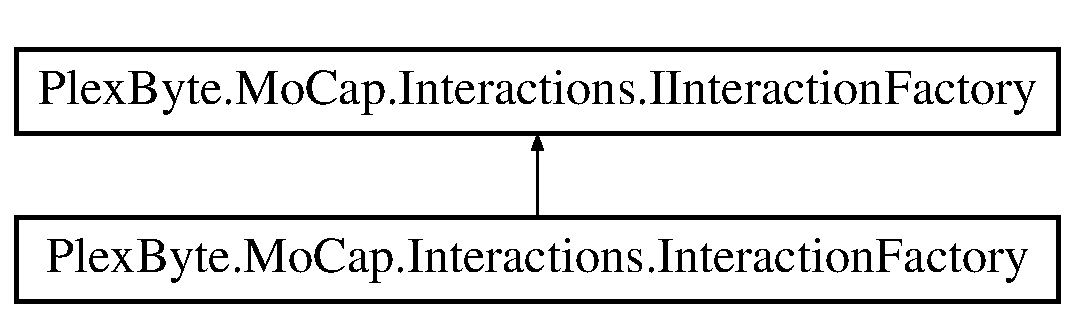
\includegraphics[height=2.000000cm]{class_plex_byte_1_1_mo_cap_1_1_interactions_1_1_interaction_factory}
\end{center}
\end{figure}
\subsection*{Public Member Functions}
\begin{DoxyCompactItemize}
\item 
virtual \hyperlink{interface_plex_byte_1_1_mo_cap_1_1_interactions_1_1_i_task}{I\+Task} \hyperlink{class_plex_byte_1_1_mo_cap_1_1_interactions_1_1_interaction_factory_a9a7f2eed60a838269aa2a4444e50ecef}{Create\+Task} (string p\+Id, string p\+Text, I\+User p\+Creator)
\item 
virtual \hyperlink{interface_plex_byte_1_1_mo_cap_1_1_interactions_1_1_i_task}{I\+Task} \hyperlink{class_plex_byte_1_1_mo_cap_1_1_interactions_1_1_interaction_factory_ab49d25714033edffd3bd5c87e453a237}{Create\+Task} (string p\+Id, string p\+Text, I\+User p\+Creator, Date\+Time p\+Start\+DT, Date\+Time p\+End\+DT, Date\+Time p\+Due\+DT)
\item 
\hyperlink{interface_plex_byte_1_1_mo_cap_1_1_interactions_1_1_i_task}{I\+Task} \hyperlink{class_plex_byte_1_1_mo_cap_1_1_interactions_1_1_interaction_factory_a1e9890e2e67cca051f1485f453a3c760}{Create\+Task} (string p\+Id, string p\+Text, I\+User p\+Creator, Date\+Time p\+Start\+DT, Date\+Time p\+End\+DT, Date\+Time p\+Due\+DT, decimal p\+Budget, int p\+Duration, int p\+Priority, \hyperlink{namespace_plex_byte_1_1_mo_cap_1_1_interactions_afcb673d9186608b6bd3b187179aedc8a}{Interaction\+State} p\+State, decimal p\+Budget\+Used, int p\+Time\+Used, List$<$ \hyperlink{interface_plex_byte_1_1_mo_cap_1_1_interactions_1_1_i_task}{I\+Task} $>$ p\+Sub\+Task, int p\+Progress)
\item 
\hyperlink{interface_plex_byte_1_1_mo_cap_1_1_interactions_1_1_i_task}{I\+Task} \hyperlink{class_plex_byte_1_1_mo_cap_1_1_interactions_1_1_interaction_factory_a030a74854486e68be1cb97166214ef16}{Create\+Task} (string p\+Id, string p\+Text, string p\+Title, I\+User p\+Creator, Date\+Time p\+Start\+DT, Date\+Time p\+End\+DT, Date\+Time p\+Due\+DT, decimal p\+Budget, int p\+Duration, int p\+Priority, \hyperlink{namespace_plex_byte_1_1_mo_cap_1_1_interactions_afcb673d9186608b6bd3b187179aedc8a}{Interaction\+State} p\+State, decimal p\+Budget\+Used, int p\+Time\+Used, List$<$ \hyperlink{interface_plex_byte_1_1_mo_cap_1_1_interactions_1_1_i_task}{I\+Task} $>$ p\+Sub\+Task, int p\+Progress)
\item 
virtual \hyperlink{interface_plex_byte_1_1_mo_cap_1_1_interactions_1_1_i_survey}{I\+Survey} \hyperlink{class_plex_byte_1_1_mo_cap_1_1_interactions_1_1_interaction_factory_a91bccc9e26b2a3ebdf9210f88e12777f}{Create\+Survey} (string p\+Id, string p\+Text, List$<$ \hyperlink{interface_plex_byte_1_1_mo_cap_1_1_interactions_1_1_i_survey_option}{I\+Survey\+Option} $>$ p\+Options, I\+User p\+Creator, Date\+Time p\+Start\+DT, Date\+Time p\+End\+DT, Date\+Time p\+Due\+DT, int p\+Votes\+Per\+User, string p\+Title, \hyperlink{namespace_plex_byte_1_1_mo_cap_1_1_interactions_afcb673d9186608b6bd3b187179aedc8a}{Interaction\+State} p\+State, List$<$ \hyperlink{interface_plex_byte_1_1_mo_cap_1_1_interactions_1_1_i_vote}{I\+Vote} $>$ p\+Votes)
\item 
virtual \hyperlink{interface_plex_byte_1_1_mo_cap_1_1_interactions_1_1_i_survey}{I\+Survey} \hyperlink{class_plex_byte_1_1_mo_cap_1_1_interactions_1_1_interaction_factory_a7cca7832aa0ee7ac17fa5f0339eeed2c}{Create\+Survey} (string p\+Id, string p\+Text, List$<$ string $>$ p\+Options, I\+User p\+Creator)
\item 
virtual \hyperlink{interface_plex_byte_1_1_mo_cap_1_1_interactions_1_1_i_account}{I\+Account} \hyperlink{class_plex_byte_1_1_mo_cap_1_1_interactions_1_1_interaction_factory_a08413bc140420733e410b17c2262e7ee}{Create\+Account} (string p\+Id, string p\+Text, I\+User p\+Creator)
\item 
virtual \hyperlink{interface_plex_byte_1_1_mo_cap_1_1_interactions_1_1_i_account}{I\+Account} \hyperlink{class_plex_byte_1_1_mo_cap_1_1_interactions_1_1_interaction_factory_a1d79c272ff2a70b71f7c8188756a0ae8}{Create\+Account} (string p\+Id, string p\+Text, List$<$ \hyperlink{interface_plex_byte_1_1_mo_cap_1_1_interactions_1_1_i_expense}{I\+Expense} $>$ p\+Expense\+List, List$<$ \hyperlink{interface_plex_byte_1_1_mo_cap_1_1_interactions_1_1_i_timeslice}{I\+Timeslice} $>$ p\+Timeslice\+List, I\+User p\+Creator)
\item 
virtual \hyperlink{interface_plex_byte_1_1_mo_cap_1_1_interactions_1_1_i_timeslice}{I\+Timeslice} \hyperlink{class_plex_byte_1_1_mo_cap_1_1_interactions_1_1_interaction_factory_a09b8c47419a3eefd5823056f72c47130}{Create\+Timeslice} (string p\+Id, I\+User p\+User, Date\+Time p\+Start\+DT, Date\+Time p\+End\+DT, \hyperlink{interface_plex_byte_1_1_mo_cap_1_1_interactions_1_1_i_interaction}{I\+Interaction} p\+Target)
\item 
virtual \hyperlink{interface_plex_byte_1_1_mo_cap_1_1_interactions_1_1_i_timeslice}{I\+Timeslice} \hyperlink{class_plex_byte_1_1_mo_cap_1_1_interactions_1_1_interaction_factory_a66108b416dc8f455fd0dc22123b2d143}{Create\+Timeslice} (string p\+Id, I\+User p\+User, int p\+Duration, \hyperlink{interface_plex_byte_1_1_mo_cap_1_1_interactions_1_1_i_interaction}{I\+Interaction} p\+Target)
\item 
virtual \hyperlink{interface_plex_byte_1_1_mo_cap_1_1_interactions_1_1_i_expense}{I\+Expense} \hyperlink{class_plex_byte_1_1_mo_cap_1_1_interactions_1_1_interaction_factory_a6d6a4839a754494e5db0adbb69fccc94}{Create\+Expense} (string p\+Id, string p\+Text, System.\+Drawing.\+Image p\+Receipt, decimal p\+Value, I\+User p\+User, \hyperlink{interface_plex_byte_1_1_mo_cap_1_1_interactions_1_1_i_interaction}{I\+Interaction} p\+Target)
\item 
virtual \hyperlink{interface_plex_byte_1_1_mo_cap_1_1_interactions_1_1_i_expense}{I\+Expense} \hyperlink{class_plex_byte_1_1_mo_cap_1_1_interactions_1_1_interaction_factory_a40751419f32c51ae9cfa556b22c8fd7f}{Create\+Expense} (string p\+Id, string p\+Text, I\+User p\+User, \hyperlink{interface_plex_byte_1_1_mo_cap_1_1_interactions_1_1_i_interaction}{I\+Interaction} p\+Target)
\item 
virtual \hyperlink{interface_plex_byte_1_1_mo_cap_1_1_interactions_1_1_i_project}{I\+Project} \hyperlink{class_plex_byte_1_1_mo_cap_1_1_interactions_1_1_interaction_factory_a38a010ef1a5e042ccbb1250adaa2324d}{Create\+Project} (string p\+Id, string p\+Text, bool p\+Enable\+Balance, bool p\+Enable\+Survey, Date\+Time p\+Start\+DT, Date\+Time p\+End\+DT, I\+User p\+Creator)
\item 
virtual \hyperlink{interface_plex_byte_1_1_mo_cap_1_1_interactions_1_1_i_project}{I\+Project} \hyperlink{class_plex_byte_1_1_mo_cap_1_1_interactions_1_1_interaction_factory_ab8dddf10ff7dd5720603c1859d96a78d}{Create\+Project} (string p\+Id, string p\+Text, bool p\+Enable\+Balance, bool p\+Enable\+Survey, Date\+Time p\+Start\+DT, Date\+Time p\+End\+DT, I\+User p\+Creator, I\+User p\+Owner, List$<$ I\+User $>$ p\+Member\+List, List$<$ I\+User $>$ p\+Invitation\+List, List$<$ \hyperlink{interface_plex_byte_1_1_mo_cap_1_1_interactions_1_1_i_task}{I\+Task} $>$ p\+Task\+List, List$<$ \hyperlink{interface_plex_byte_1_1_mo_cap_1_1_interactions_1_1_i_survey}{I\+Survey} $>$ p\+Survey\+List, string p\+Name)
\item 
virtual \hyperlink{interface_plex_byte_1_1_mo_cap_1_1_interactions_1_1_i_interaction}{I\+Interaction} \hyperlink{class_plex_byte_1_1_mo_cap_1_1_interactions_1_1_interaction_factory_a8499cf461c2028c8e47f61056856a47d}{Create\+Chat} (string p\+Text\+Title, I\+User p\+Creator, List$<$ I\+User $>$ p\+Users)
\item 
virtual \hyperlink{interface_plex_byte_1_1_mo_cap_1_1_interactions_1_1_i_interaction}{I\+Interaction} \hyperlink{class_plex_byte_1_1_mo_cap_1_1_interactions_1_1_interaction_factory_a90e50fa9b778353e619c059ea5b78822}{Create\+Chat} (string p\+Text\+Title, I\+User p\+Creator, List$<$ I\+User $>$ p\+Users, Date\+Time p\+Start\+Date\+Time, Date\+Time p\+End\+Date\+Time, bool p\+Allow\+Selfdestructing)
\item 
virtual \hyperlink{interface_plex_byte_1_1_mo_cap_1_1_interactions_1_1_i_interaction}{I\+Interaction} \hyperlink{class_plex_byte_1_1_mo_cap_1_1_interactions_1_1_interaction_factory_a43297682c502977cf7ebc69a9fe8b15f}{Create\+Interaction} (string p\+Id, Date\+Time p\+Start\+Date\+Time, Date\+Time p\+End\+Date\+Time, bool p\+Is\+Active, string p\+Text, \hyperlink{namespace_plex_byte_1_1_mo_cap_1_1_interactions_a6e7bea333446664bbce2bb296db25e31}{Interaction\+Type} p\+Type, \hyperlink{namespace_plex_byte_1_1_mo_cap_1_1_interactions_afcb673d9186608b6bd3b187179aedc8a}{Interaction\+State} p\+State, I\+User p\+Owner, I\+User p\+Creator, Date\+Time p\+Created, Date\+Time p\+Modified)
\end{DoxyCompactItemize}


\subsection{Detailed Description}


Definition at line 14 of file Interaction\+Factory.\+cs.



\subsection{Member Function Documentation}
\index{Plex\+Byte\+::\+Mo\+Cap\+::\+Interactions\+::\+Interaction\+Factory@{Plex\+Byte\+::\+Mo\+Cap\+::\+Interactions\+::\+Interaction\+Factory}!Create\+Account@{Create\+Account}}
\index{Create\+Account@{Create\+Account}!Plex\+Byte\+::\+Mo\+Cap\+::\+Interactions\+::\+Interaction\+Factory@{Plex\+Byte\+::\+Mo\+Cap\+::\+Interactions\+::\+Interaction\+Factory}}
\subsubsection[{\texorpdfstring{Create\+Account(string p\+Id, string p\+Text, I\+User p\+Creator)}{CreateAccount(string pId, string pText, IUser pCreator)}}]{\setlength{\rightskip}{0pt plus 5cm}virtual {\bf I\+Account} Plex\+Byte.\+Mo\+Cap.\+Interactions.\+Interaction\+Factory.\+Create\+Account (
\begin{DoxyParamCaption}
\item[{string}]{p\+Id, }
\item[{string}]{p\+Text, }
\item[{I\+User}]{p\+Creator}
\end{DoxyParamCaption}
)\hspace{0.3cm}{\ttfamily [virtual]}}\hypertarget{class_plex_byte_1_1_mo_cap_1_1_interactions_1_1_interaction_factory_a08413bc140420733e410b17c2262e7ee}{}\label{class_plex_byte_1_1_mo_cap_1_1_interactions_1_1_interaction_factory_a08413bc140420733e410b17c2262e7ee}


Implements \hyperlink{interface_plex_byte_1_1_mo_cap_1_1_interactions_1_1_i_interaction_factory_ad30e523a2735f42e372375250a1dc025}{Plex\+Byte.\+Mo\+Cap.\+Interactions.\+I\+Interaction\+Factory}.



Definition at line 133 of file Interaction\+Factory.\+cs.

\index{Plex\+Byte\+::\+Mo\+Cap\+::\+Interactions\+::\+Interaction\+Factory@{Plex\+Byte\+::\+Mo\+Cap\+::\+Interactions\+::\+Interaction\+Factory}!Create\+Account@{Create\+Account}}
\index{Create\+Account@{Create\+Account}!Plex\+Byte\+::\+Mo\+Cap\+::\+Interactions\+::\+Interaction\+Factory@{Plex\+Byte\+::\+Mo\+Cap\+::\+Interactions\+::\+Interaction\+Factory}}
\subsubsection[{\texorpdfstring{Create\+Account(string p\+Id, string p\+Text, List$<$ I\+Expense $>$ p\+Expense\+List, List$<$ I\+Timeslice $>$ p\+Timeslice\+List, I\+User p\+Creator)}{CreateAccount(string pId, string pText, List< IExpense > pExpenseList, List< ITimeslice > pTimesliceList, IUser pCreator)}}]{\setlength{\rightskip}{0pt plus 5cm}virtual {\bf I\+Account} Plex\+Byte.\+Mo\+Cap.\+Interactions.\+Interaction\+Factory.\+Create\+Account (
\begin{DoxyParamCaption}
\item[{string}]{p\+Id, }
\item[{string}]{p\+Text, }
\item[{List$<$ {\bf I\+Expense} $>$}]{p\+Expense\+List, }
\item[{List$<$ {\bf I\+Timeslice} $>$}]{p\+Timeslice\+List, }
\item[{I\+User}]{p\+Creator}
\end{DoxyParamCaption}
)\hspace{0.3cm}{\ttfamily [virtual]}}\hypertarget{class_plex_byte_1_1_mo_cap_1_1_interactions_1_1_interaction_factory_a1d79c272ff2a70b71f7c8188756a0ae8}{}\label{class_plex_byte_1_1_mo_cap_1_1_interactions_1_1_interaction_factory_a1d79c272ff2a70b71f7c8188756a0ae8}


Implements \hyperlink{interface_plex_byte_1_1_mo_cap_1_1_interactions_1_1_i_interaction_factory_a4909855456dce1184abdb5dd2d8a679d}{Plex\+Byte.\+Mo\+Cap.\+Interactions.\+I\+Interaction\+Factory}.



Definition at line 140 of file Interaction\+Factory.\+cs.

\index{Plex\+Byte\+::\+Mo\+Cap\+::\+Interactions\+::\+Interaction\+Factory@{Plex\+Byte\+::\+Mo\+Cap\+::\+Interactions\+::\+Interaction\+Factory}!Create\+Chat@{Create\+Chat}}
\index{Create\+Chat@{Create\+Chat}!Plex\+Byte\+::\+Mo\+Cap\+::\+Interactions\+::\+Interaction\+Factory@{Plex\+Byte\+::\+Mo\+Cap\+::\+Interactions\+::\+Interaction\+Factory}}
\subsubsection[{\texorpdfstring{Create\+Chat(string p\+Text\+Title, I\+User p\+Creator, List$<$ I\+User $>$ p\+Users)}{CreateChat(string pTextTitle, IUser pCreator, List< IUser > pUsers)}}]{\setlength{\rightskip}{0pt plus 5cm}virtual {\bf I\+Interaction} Plex\+Byte.\+Mo\+Cap.\+Interactions.\+Interaction\+Factory.\+Create\+Chat (
\begin{DoxyParamCaption}
\item[{string}]{p\+Text\+Title, }
\item[{I\+User}]{p\+Creator, }
\item[{List$<$ I\+User $>$}]{p\+Users}
\end{DoxyParamCaption}
)\hspace{0.3cm}{\ttfamily [virtual]}}\hypertarget{class_plex_byte_1_1_mo_cap_1_1_interactions_1_1_interaction_factory_a8499cf461c2028c8e47f61056856a47d}{}\label{class_plex_byte_1_1_mo_cap_1_1_interactions_1_1_interaction_factory_a8499cf461c2028c8e47f61056856a47d}


Implements \hyperlink{interface_plex_byte_1_1_mo_cap_1_1_interactions_1_1_i_interaction_factory_aabee33e1d8b7c8106b543dc52b218782}{Plex\+Byte.\+Mo\+Cap.\+Interactions.\+I\+Interaction\+Factory}.



Definition at line 193 of file Interaction\+Factory.\+cs.

\index{Plex\+Byte\+::\+Mo\+Cap\+::\+Interactions\+::\+Interaction\+Factory@{Plex\+Byte\+::\+Mo\+Cap\+::\+Interactions\+::\+Interaction\+Factory}!Create\+Chat@{Create\+Chat}}
\index{Create\+Chat@{Create\+Chat}!Plex\+Byte\+::\+Mo\+Cap\+::\+Interactions\+::\+Interaction\+Factory@{Plex\+Byte\+::\+Mo\+Cap\+::\+Interactions\+::\+Interaction\+Factory}}
\subsubsection[{\texorpdfstring{Create\+Chat(string p\+Text\+Title, I\+User p\+Creator, List$<$ I\+User $>$ p\+Users, Date\+Time p\+Start\+Date\+Time, Date\+Time p\+End\+Date\+Time, bool p\+Allow\+Selfdestructing)}{CreateChat(string pTextTitle, IUser pCreator, List< IUser > pUsers, DateTime pStartDateTime, DateTime pEndDateTime, bool pAllowSelfdestructing)}}]{\setlength{\rightskip}{0pt plus 5cm}virtual {\bf I\+Interaction} Plex\+Byte.\+Mo\+Cap.\+Interactions.\+Interaction\+Factory.\+Create\+Chat (
\begin{DoxyParamCaption}
\item[{string}]{p\+Text\+Title, }
\item[{I\+User}]{p\+Creator, }
\item[{List$<$ I\+User $>$}]{p\+Users, }
\item[{Date\+Time}]{p\+Start\+Date\+Time, }
\item[{Date\+Time}]{p\+End\+Date\+Time, }
\item[{bool}]{p\+Allow\+Selfdestructing}
\end{DoxyParamCaption}
)\hspace{0.3cm}{\ttfamily [virtual]}}\hypertarget{class_plex_byte_1_1_mo_cap_1_1_interactions_1_1_interaction_factory_a90e50fa9b778353e619c059ea5b78822}{}\label{class_plex_byte_1_1_mo_cap_1_1_interactions_1_1_interaction_factory_a90e50fa9b778353e619c059ea5b78822}


Implements \hyperlink{interface_plex_byte_1_1_mo_cap_1_1_interactions_1_1_i_interaction_factory_a41eeaa8cf6c81e669898eb2b4d57eb9b}{Plex\+Byte.\+Mo\+Cap.\+Interactions.\+I\+Interaction\+Factory}.



Definition at line 195 of file Interaction\+Factory.\+cs.

\index{Plex\+Byte\+::\+Mo\+Cap\+::\+Interactions\+::\+Interaction\+Factory@{Plex\+Byte\+::\+Mo\+Cap\+::\+Interactions\+::\+Interaction\+Factory}!Create\+Expense@{Create\+Expense}}
\index{Create\+Expense@{Create\+Expense}!Plex\+Byte\+::\+Mo\+Cap\+::\+Interactions\+::\+Interaction\+Factory@{Plex\+Byte\+::\+Mo\+Cap\+::\+Interactions\+::\+Interaction\+Factory}}
\subsubsection[{\texorpdfstring{Create\+Expense(string p\+Id, string p\+Text, System.\+Drawing.\+Image p\+Receipt, decimal p\+Value, I\+User p\+User, I\+Interaction p\+Target)}{CreateExpense(string pId, string pText, System.Drawing.Image pReceipt, decimal pValue, IUser pUser, IInteraction pTarget)}}]{\setlength{\rightskip}{0pt plus 5cm}virtual {\bf I\+Expense} Plex\+Byte.\+Mo\+Cap.\+Interactions.\+Interaction\+Factory.\+Create\+Expense (
\begin{DoxyParamCaption}
\item[{string}]{p\+Id, }
\item[{string}]{p\+Text, }
\item[{System.\+Drawing.\+Image}]{p\+Receipt, }
\item[{decimal}]{p\+Value, }
\item[{I\+User}]{p\+User, }
\item[{{\bf I\+Interaction}}]{p\+Target}
\end{DoxyParamCaption}
)\hspace{0.3cm}{\ttfamily [virtual]}}\hypertarget{class_plex_byte_1_1_mo_cap_1_1_interactions_1_1_interaction_factory_a6d6a4839a754494e5db0adbb69fccc94}{}\label{class_plex_byte_1_1_mo_cap_1_1_interactions_1_1_interaction_factory_a6d6a4839a754494e5db0adbb69fccc94}


Implements \hyperlink{interface_plex_byte_1_1_mo_cap_1_1_interactions_1_1_i_interaction_factory_ac85fb39c0c3072a8421e4fb3b39359cd}{Plex\+Byte.\+Mo\+Cap.\+Interactions.\+I\+Interaction\+Factory}.



Definition at line 165 of file Interaction\+Factory.\+cs.

\index{Plex\+Byte\+::\+Mo\+Cap\+::\+Interactions\+::\+Interaction\+Factory@{Plex\+Byte\+::\+Mo\+Cap\+::\+Interactions\+::\+Interaction\+Factory}!Create\+Expense@{Create\+Expense}}
\index{Create\+Expense@{Create\+Expense}!Plex\+Byte\+::\+Mo\+Cap\+::\+Interactions\+::\+Interaction\+Factory@{Plex\+Byte\+::\+Mo\+Cap\+::\+Interactions\+::\+Interaction\+Factory}}
\subsubsection[{\texorpdfstring{Create\+Expense(string p\+Id, string p\+Text, I\+User p\+User, I\+Interaction p\+Target)}{CreateExpense(string pId, string pText, IUser pUser, IInteraction pTarget)}}]{\setlength{\rightskip}{0pt plus 5cm}virtual {\bf I\+Expense} Plex\+Byte.\+Mo\+Cap.\+Interactions.\+Interaction\+Factory.\+Create\+Expense (
\begin{DoxyParamCaption}
\item[{string}]{p\+Id, }
\item[{string}]{p\+Text, }
\item[{I\+User}]{p\+User, }
\item[{{\bf I\+Interaction}}]{p\+Target}
\end{DoxyParamCaption}
)\hspace{0.3cm}{\ttfamily [virtual]}}\hypertarget{class_plex_byte_1_1_mo_cap_1_1_interactions_1_1_interaction_factory_a40751419f32c51ae9cfa556b22c8fd7f}{}\label{class_plex_byte_1_1_mo_cap_1_1_interactions_1_1_interaction_factory_a40751419f32c51ae9cfa556b22c8fd7f}


Implements \hyperlink{interface_plex_byte_1_1_mo_cap_1_1_interactions_1_1_i_interaction_factory_a0d7c926ff7b8d7c07bdc143919f3a0f7}{Plex\+Byte.\+Mo\+Cap.\+Interactions.\+I\+Interaction\+Factory}.



Definition at line 172 of file Interaction\+Factory.\+cs.

\index{Plex\+Byte\+::\+Mo\+Cap\+::\+Interactions\+::\+Interaction\+Factory@{Plex\+Byte\+::\+Mo\+Cap\+::\+Interactions\+::\+Interaction\+Factory}!Create\+Interaction@{Create\+Interaction}}
\index{Create\+Interaction@{Create\+Interaction}!Plex\+Byte\+::\+Mo\+Cap\+::\+Interactions\+::\+Interaction\+Factory@{Plex\+Byte\+::\+Mo\+Cap\+::\+Interactions\+::\+Interaction\+Factory}}
\subsubsection[{\texorpdfstring{Create\+Interaction(string p\+Id, Date\+Time p\+Start\+Date\+Time, Date\+Time p\+End\+Date\+Time, bool p\+Is\+Active, string p\+Text, Interaction\+Type p\+Type, Interaction\+State p\+State, I\+User p\+Owner, I\+User p\+Creator, Date\+Time p\+Created, Date\+Time p\+Modified)}{CreateInteraction(string pId, DateTime pStartDateTime, DateTime pEndDateTime, bool pIsActive, string pText, InteractionType pType, InteractionState pState, IUser pOwner, IUser pCreator, DateTime pCreated, DateTime pModified)}}]{\setlength{\rightskip}{0pt plus 5cm}virtual {\bf I\+Interaction} Plex\+Byte.\+Mo\+Cap.\+Interactions.\+Interaction\+Factory.\+Create\+Interaction (
\begin{DoxyParamCaption}
\item[{string}]{p\+Id, }
\item[{Date\+Time}]{p\+Start\+Date\+Time, }
\item[{Date\+Time}]{p\+End\+Date\+Time, }
\item[{bool}]{p\+Is\+Active, }
\item[{string}]{p\+Text, }
\item[{{\bf Interaction\+Type}}]{p\+Type, }
\item[{{\bf Interaction\+State}}]{p\+State, }
\item[{I\+User}]{p\+Owner, }
\item[{I\+User}]{p\+Creator, }
\item[{Date\+Time}]{p\+Created, }
\item[{Date\+Time}]{p\+Modified}
\end{DoxyParamCaption}
)\hspace{0.3cm}{\ttfamily [virtual]}}\hypertarget{class_plex_byte_1_1_mo_cap_1_1_interactions_1_1_interaction_factory_a43297682c502977cf7ebc69a9fe8b15f}{}\label{class_plex_byte_1_1_mo_cap_1_1_interactions_1_1_interaction_factory_a43297682c502977cf7ebc69a9fe8b15f}


Implements \hyperlink{interface_plex_byte_1_1_mo_cap_1_1_interactions_1_1_i_interaction_factory_a7a9e3fc490901c3a0be3faadadb27494}{Plex\+Byte.\+Mo\+Cap.\+Interactions.\+I\+Interaction\+Factory}.



Definition at line 205 of file Interaction\+Factory.\+cs.

\index{Plex\+Byte\+::\+Mo\+Cap\+::\+Interactions\+::\+Interaction\+Factory@{Plex\+Byte\+::\+Mo\+Cap\+::\+Interactions\+::\+Interaction\+Factory}!Create\+Project@{Create\+Project}}
\index{Create\+Project@{Create\+Project}!Plex\+Byte\+::\+Mo\+Cap\+::\+Interactions\+::\+Interaction\+Factory@{Plex\+Byte\+::\+Mo\+Cap\+::\+Interactions\+::\+Interaction\+Factory}}
\subsubsection[{\texorpdfstring{Create\+Project(string p\+Id, string p\+Text, bool p\+Enable\+Balance, bool p\+Enable\+Survey, Date\+Time p\+Start\+D\+T, Date\+Time p\+End\+D\+T, I\+User p\+Creator)}{CreateProject(string pId, string pText, bool pEnableBalance, bool pEnableSurvey, DateTime pStartDT, DateTime pEndDT, IUser pCreator)}}]{\setlength{\rightskip}{0pt plus 5cm}virtual {\bf I\+Project} Plex\+Byte.\+Mo\+Cap.\+Interactions.\+Interaction\+Factory.\+Create\+Project (
\begin{DoxyParamCaption}
\item[{string}]{p\+Id, }
\item[{string}]{p\+Text, }
\item[{bool}]{p\+Enable\+Balance, }
\item[{bool}]{p\+Enable\+Survey, }
\item[{Date\+Time}]{p\+Start\+DT, }
\item[{Date\+Time}]{p\+End\+DT, }
\item[{I\+User}]{p\+Creator}
\end{DoxyParamCaption}
)\hspace{0.3cm}{\ttfamily [virtual]}}\hypertarget{class_plex_byte_1_1_mo_cap_1_1_interactions_1_1_interaction_factory_a38a010ef1a5e042ccbb1250adaa2324d}{}\label{class_plex_byte_1_1_mo_cap_1_1_interactions_1_1_interaction_factory_a38a010ef1a5e042ccbb1250adaa2324d}


Implements \hyperlink{interface_plex_byte_1_1_mo_cap_1_1_interactions_1_1_i_interaction_factory_a185e39ef7292fa875c3e60eead0eb1d7}{Plex\+Byte.\+Mo\+Cap.\+Interactions.\+I\+Interaction\+Factory}.



Definition at line 179 of file Interaction\+Factory.\+cs.

\index{Plex\+Byte\+::\+Mo\+Cap\+::\+Interactions\+::\+Interaction\+Factory@{Plex\+Byte\+::\+Mo\+Cap\+::\+Interactions\+::\+Interaction\+Factory}!Create\+Project@{Create\+Project}}
\index{Create\+Project@{Create\+Project}!Plex\+Byte\+::\+Mo\+Cap\+::\+Interactions\+::\+Interaction\+Factory@{Plex\+Byte\+::\+Mo\+Cap\+::\+Interactions\+::\+Interaction\+Factory}}
\subsubsection[{\texorpdfstring{Create\+Project(string p\+Id, string p\+Text, bool p\+Enable\+Balance, bool p\+Enable\+Survey, Date\+Time p\+Start\+D\+T, Date\+Time p\+End\+D\+T, I\+User p\+Creator, I\+User p\+Owner, List$<$ I\+User $>$ p\+Member\+List, List$<$ I\+User $>$ p\+Invitation\+List, List$<$ I\+Task $>$ p\+Task\+List, List$<$ I\+Survey $>$ p\+Survey\+List, string p\+Name)}{CreateProject(string pId, string pText, bool pEnableBalance, bool pEnableSurvey, DateTime pStartDT, DateTime pEndDT, IUser pCreator, IUser pOwner, List< IUser > pMemberList, List< IUser > pInvitationList, List< ITask > pTaskList, List< ISurvey > pSurveyList, string pName)}}]{\setlength{\rightskip}{0pt plus 5cm}virtual {\bf I\+Project} Plex\+Byte.\+Mo\+Cap.\+Interactions.\+Interaction\+Factory.\+Create\+Project (
\begin{DoxyParamCaption}
\item[{string}]{p\+Id, }
\item[{string}]{p\+Text, }
\item[{bool}]{p\+Enable\+Balance, }
\item[{bool}]{p\+Enable\+Survey, }
\item[{Date\+Time}]{p\+Start\+DT, }
\item[{Date\+Time}]{p\+End\+DT, }
\item[{I\+User}]{p\+Creator, }
\item[{I\+User}]{p\+Owner, }
\item[{List$<$ I\+User $>$}]{p\+Member\+List, }
\item[{List$<$ I\+User $>$}]{p\+Invitation\+List, }
\item[{List$<$ {\bf I\+Task} $>$}]{p\+Task\+List, }
\item[{List$<$ {\bf I\+Survey} $>$}]{p\+Survey\+List, }
\item[{string}]{p\+Name}
\end{DoxyParamCaption}
)\hspace{0.3cm}{\ttfamily [virtual]}}\hypertarget{class_plex_byte_1_1_mo_cap_1_1_interactions_1_1_interaction_factory_ab8dddf10ff7dd5720603c1859d96a78d}{}\label{class_plex_byte_1_1_mo_cap_1_1_interactions_1_1_interaction_factory_ab8dddf10ff7dd5720603c1859d96a78d}


Implements \hyperlink{interface_plex_byte_1_1_mo_cap_1_1_interactions_1_1_i_interaction_factory_a96f9a4cfec44b654fedcc3e62fe617ca}{Plex\+Byte.\+Mo\+Cap.\+Interactions.\+I\+Interaction\+Factory}.



Definition at line 186 of file Interaction\+Factory.\+cs.

\index{Plex\+Byte\+::\+Mo\+Cap\+::\+Interactions\+::\+Interaction\+Factory@{Plex\+Byte\+::\+Mo\+Cap\+::\+Interactions\+::\+Interaction\+Factory}!Create\+Survey@{Create\+Survey}}
\index{Create\+Survey@{Create\+Survey}!Plex\+Byte\+::\+Mo\+Cap\+::\+Interactions\+::\+Interaction\+Factory@{Plex\+Byte\+::\+Mo\+Cap\+::\+Interactions\+::\+Interaction\+Factory}}
\subsubsection[{\texorpdfstring{Create\+Survey(string p\+Id, string p\+Text, List$<$ I\+Survey\+Option $>$ p\+Options, I\+User p\+Creator, Date\+Time p\+Start\+D\+T, Date\+Time p\+End\+D\+T, Date\+Time p\+Due\+D\+T, int p\+Votes\+Per\+User, string p\+Title, Interaction\+State p\+State, List$<$ I\+Vote $>$ p\+Votes)}{CreateSurvey(string pId, string pText, List< ISurveyOption > pOptions, IUser pCreator, DateTime pStartDT, DateTime pEndDT, DateTime pDueDT, int pVotesPerUser, string pTitle, InteractionState pState, List< IVote > pVotes)}}]{\setlength{\rightskip}{0pt plus 5cm}virtual {\bf I\+Survey} Plex\+Byte.\+Mo\+Cap.\+Interactions.\+Interaction\+Factory.\+Create\+Survey (
\begin{DoxyParamCaption}
\item[{string}]{p\+Id, }
\item[{string}]{p\+Text, }
\item[{List$<$ {\bf I\+Survey\+Option} $>$}]{p\+Options, }
\item[{I\+User}]{p\+Creator, }
\item[{Date\+Time}]{p\+Start\+DT, }
\item[{Date\+Time}]{p\+End\+DT, }
\item[{Date\+Time}]{p\+Due\+DT, }
\item[{int}]{p\+Votes\+Per\+User, }
\item[{string}]{p\+Title, }
\item[{{\bf Interaction\+State}}]{p\+State, }
\item[{List$<$ {\bf I\+Vote} $>$}]{p\+Votes}
\end{DoxyParamCaption}
)\hspace{0.3cm}{\ttfamily [virtual]}}\hypertarget{class_plex_byte_1_1_mo_cap_1_1_interactions_1_1_interaction_factory_a91bccc9e26b2a3ebdf9210f88e12777f}{}\label{class_plex_byte_1_1_mo_cap_1_1_interactions_1_1_interaction_factory_a91bccc9e26b2a3ebdf9210f88e12777f}


Implements \hyperlink{interface_plex_byte_1_1_mo_cap_1_1_interactions_1_1_i_interaction_factory_a10d691633579fc9ebef747595e09a1c2}{Plex\+Byte.\+Mo\+Cap.\+Interactions.\+I\+Interaction\+Factory}.



Definition at line 104 of file Interaction\+Factory.\+cs.

\index{Plex\+Byte\+::\+Mo\+Cap\+::\+Interactions\+::\+Interaction\+Factory@{Plex\+Byte\+::\+Mo\+Cap\+::\+Interactions\+::\+Interaction\+Factory}!Create\+Survey@{Create\+Survey}}
\index{Create\+Survey@{Create\+Survey}!Plex\+Byte\+::\+Mo\+Cap\+::\+Interactions\+::\+Interaction\+Factory@{Plex\+Byte\+::\+Mo\+Cap\+::\+Interactions\+::\+Interaction\+Factory}}
\subsubsection[{\texorpdfstring{Create\+Survey(string p\+Id, string p\+Text, List$<$ string $>$ p\+Options, I\+User p\+Creator)}{CreateSurvey(string pId, string pText, List< string > pOptions, IUser pCreator)}}]{\setlength{\rightskip}{0pt plus 5cm}virtual {\bf I\+Survey} Plex\+Byte.\+Mo\+Cap.\+Interactions.\+Interaction\+Factory.\+Create\+Survey (
\begin{DoxyParamCaption}
\item[{string}]{p\+Id, }
\item[{string}]{p\+Text, }
\item[{List$<$ string $>$}]{p\+Options, }
\item[{I\+User}]{p\+Creator}
\end{DoxyParamCaption}
)\hspace{0.3cm}{\ttfamily [virtual]}}\hypertarget{class_plex_byte_1_1_mo_cap_1_1_interactions_1_1_interaction_factory_a7cca7832aa0ee7ac17fa5f0339eeed2c}{}\label{class_plex_byte_1_1_mo_cap_1_1_interactions_1_1_interaction_factory_a7cca7832aa0ee7ac17fa5f0339eeed2c}


Implements \hyperlink{interface_plex_byte_1_1_mo_cap_1_1_interactions_1_1_i_interaction_factory_a5b5cedeba1e0748c243b7a9a5f2fb5a6}{Plex\+Byte.\+Mo\+Cap.\+Interactions.\+I\+Interaction\+Factory}.



Definition at line 126 of file Interaction\+Factory.\+cs.

\index{Plex\+Byte\+::\+Mo\+Cap\+::\+Interactions\+::\+Interaction\+Factory@{Plex\+Byte\+::\+Mo\+Cap\+::\+Interactions\+::\+Interaction\+Factory}!Create\+Task@{Create\+Task}}
\index{Create\+Task@{Create\+Task}!Plex\+Byte\+::\+Mo\+Cap\+::\+Interactions\+::\+Interaction\+Factory@{Plex\+Byte\+::\+Mo\+Cap\+::\+Interactions\+::\+Interaction\+Factory}}
\subsubsection[{\texorpdfstring{Create\+Task(string p\+Id, string p\+Text, I\+User p\+Creator)}{CreateTask(string pId, string pText, IUser pCreator)}}]{\setlength{\rightskip}{0pt plus 5cm}virtual {\bf I\+Task} Plex\+Byte.\+Mo\+Cap.\+Interactions.\+Interaction\+Factory.\+Create\+Task (
\begin{DoxyParamCaption}
\item[{string}]{p\+Id, }
\item[{string}]{p\+Text, }
\item[{I\+User}]{p\+Creator}
\end{DoxyParamCaption}
)\hspace{0.3cm}{\ttfamily [virtual]}}\hypertarget{class_plex_byte_1_1_mo_cap_1_1_interactions_1_1_interaction_factory_a9a7f2eed60a838269aa2a4444e50ecef}{}\label{class_plex_byte_1_1_mo_cap_1_1_interactions_1_1_interaction_factory_a9a7f2eed60a838269aa2a4444e50ecef}


Implements \hyperlink{interface_plex_byte_1_1_mo_cap_1_1_interactions_1_1_i_interaction_factory_a2652ae146eddd246b136bfd47b55bd10}{Plex\+Byte.\+Mo\+Cap.\+Interactions.\+I\+Interaction\+Factory}.



Definition at line 16 of file Interaction\+Factory.\+cs.

\index{Plex\+Byte\+::\+Mo\+Cap\+::\+Interactions\+::\+Interaction\+Factory@{Plex\+Byte\+::\+Mo\+Cap\+::\+Interactions\+::\+Interaction\+Factory}!Create\+Task@{Create\+Task}}
\index{Create\+Task@{Create\+Task}!Plex\+Byte\+::\+Mo\+Cap\+::\+Interactions\+::\+Interaction\+Factory@{Plex\+Byte\+::\+Mo\+Cap\+::\+Interactions\+::\+Interaction\+Factory}}
\subsubsection[{\texorpdfstring{Create\+Task(string p\+Id, string p\+Text, I\+User p\+Creator, Date\+Time p\+Start\+D\+T, Date\+Time p\+End\+D\+T, Date\+Time p\+Due\+D\+T)}{CreateTask(string pId, string pText, IUser pCreator, DateTime pStartDT, DateTime pEndDT, DateTime pDueDT)}}]{\setlength{\rightskip}{0pt plus 5cm}virtual {\bf I\+Task} Plex\+Byte.\+Mo\+Cap.\+Interactions.\+Interaction\+Factory.\+Create\+Task (
\begin{DoxyParamCaption}
\item[{string}]{p\+Id, }
\item[{string}]{p\+Text, }
\item[{I\+User}]{p\+Creator, }
\item[{Date\+Time}]{p\+Start\+DT, }
\item[{Date\+Time}]{p\+End\+DT, }
\item[{Date\+Time}]{p\+Due\+DT}
\end{DoxyParamCaption}
)\hspace{0.3cm}{\ttfamily [virtual]}}\hypertarget{class_plex_byte_1_1_mo_cap_1_1_interactions_1_1_interaction_factory_ab49d25714033edffd3bd5c87e453a237}{}\label{class_plex_byte_1_1_mo_cap_1_1_interactions_1_1_interaction_factory_ab49d25714033edffd3bd5c87e453a237}


Implements \hyperlink{interface_plex_byte_1_1_mo_cap_1_1_interactions_1_1_i_interaction_factory_ad3f030a61f41e66812ba458194a02182}{Plex\+Byte.\+Mo\+Cap.\+Interactions.\+I\+Interaction\+Factory}.



Definition at line 23 of file Interaction\+Factory.\+cs.

\index{Plex\+Byte\+::\+Mo\+Cap\+::\+Interactions\+::\+Interaction\+Factory@{Plex\+Byte\+::\+Mo\+Cap\+::\+Interactions\+::\+Interaction\+Factory}!Create\+Task@{Create\+Task}}
\index{Create\+Task@{Create\+Task}!Plex\+Byte\+::\+Mo\+Cap\+::\+Interactions\+::\+Interaction\+Factory@{Plex\+Byte\+::\+Mo\+Cap\+::\+Interactions\+::\+Interaction\+Factory}}
\subsubsection[{\texorpdfstring{Create\+Task(string p\+Id, string p\+Text, I\+User p\+Creator, Date\+Time p\+Start\+D\+T, Date\+Time p\+End\+D\+T, Date\+Time p\+Due\+D\+T, decimal p\+Budget, int p\+Duration, int p\+Priority, Interaction\+State p\+State, decimal p\+Budget\+Used, int p\+Time\+Used, List$<$ I\+Task $>$ p\+Sub\+Task, int p\+Progress)}{CreateTask(string pId, string pText, IUser pCreator, DateTime pStartDT, DateTime pEndDT, DateTime pDueDT, decimal pBudget, int pDuration, int pPriority, InteractionState pState, decimal pBudgetUsed, int pTimeUsed, List< ITask > pSubTask, int pProgress)}}]{\setlength{\rightskip}{0pt plus 5cm}{\bf I\+Task} Plex\+Byte.\+Mo\+Cap.\+Interactions.\+Interaction\+Factory.\+Create\+Task (
\begin{DoxyParamCaption}
\item[{string}]{p\+Id, }
\item[{string}]{p\+Text, }
\item[{I\+User}]{p\+Creator, }
\item[{Date\+Time}]{p\+Start\+DT, }
\item[{Date\+Time}]{p\+End\+DT, }
\item[{Date\+Time}]{p\+Due\+DT, }
\item[{decimal}]{p\+Budget, }
\item[{int}]{p\+Duration, }
\item[{int}]{p\+Priority, }
\item[{{\bf Interaction\+State}}]{p\+State, }
\item[{decimal}]{p\+Budget\+Used, }
\item[{int}]{p\+Time\+Used, }
\item[{List$<$ {\bf I\+Task} $>$}]{p\+Sub\+Task, }
\item[{int}]{p\+Progress}
\end{DoxyParamCaption}
)}\hypertarget{class_plex_byte_1_1_mo_cap_1_1_interactions_1_1_interaction_factory_a1e9890e2e67cca051f1485f453a3c760}{}\label{class_plex_byte_1_1_mo_cap_1_1_interactions_1_1_interaction_factory_a1e9890e2e67cca051f1485f453a3c760}


Definition at line 35 of file Interaction\+Factory.\+cs.

\index{Plex\+Byte\+::\+Mo\+Cap\+::\+Interactions\+::\+Interaction\+Factory@{Plex\+Byte\+::\+Mo\+Cap\+::\+Interactions\+::\+Interaction\+Factory}!Create\+Task@{Create\+Task}}
\index{Create\+Task@{Create\+Task}!Plex\+Byte\+::\+Mo\+Cap\+::\+Interactions\+::\+Interaction\+Factory@{Plex\+Byte\+::\+Mo\+Cap\+::\+Interactions\+::\+Interaction\+Factory}}
\subsubsection[{\texorpdfstring{Create\+Task(string p\+Id, string p\+Text, string p\+Title, I\+User p\+Creator, Date\+Time p\+Start\+D\+T, Date\+Time p\+End\+D\+T, Date\+Time p\+Due\+D\+T, decimal p\+Budget, int p\+Duration, int p\+Priority, Interaction\+State p\+State, decimal p\+Budget\+Used, int p\+Time\+Used, List$<$ I\+Task $>$ p\+Sub\+Task, int p\+Progress)}{CreateTask(string pId, string pText, string pTitle, IUser pCreator, DateTime pStartDT, DateTime pEndDT, DateTime pDueDT, decimal pBudget, int pDuration, int pPriority, InteractionState pState, decimal pBudgetUsed, int pTimeUsed, List< ITask > pSubTask, int pProgress)}}]{\setlength{\rightskip}{0pt plus 5cm}{\bf I\+Task} Plex\+Byte.\+Mo\+Cap.\+Interactions.\+Interaction\+Factory.\+Create\+Task (
\begin{DoxyParamCaption}
\item[{string}]{p\+Id, }
\item[{string}]{p\+Text, }
\item[{string}]{p\+Title, }
\item[{I\+User}]{p\+Creator, }
\item[{Date\+Time}]{p\+Start\+DT, }
\item[{Date\+Time}]{p\+End\+DT, }
\item[{Date\+Time}]{p\+Due\+DT, }
\item[{decimal}]{p\+Budget, }
\item[{int}]{p\+Duration, }
\item[{int}]{p\+Priority, }
\item[{{\bf Interaction\+State}}]{p\+State, }
\item[{decimal}]{p\+Budget\+Used, }
\item[{int}]{p\+Time\+Used, }
\item[{List$<$ {\bf I\+Task} $>$}]{p\+Sub\+Task, }
\item[{int}]{p\+Progress}
\end{DoxyParamCaption}
)}\hypertarget{class_plex_byte_1_1_mo_cap_1_1_interactions_1_1_interaction_factory_a030a74854486e68be1cb97166214ef16}{}\label{class_plex_byte_1_1_mo_cap_1_1_interactions_1_1_interaction_factory_a030a74854486e68be1cb97166214ef16}


Implements \hyperlink{interface_plex_byte_1_1_mo_cap_1_1_interactions_1_1_i_interaction_factory_a36f7e9ea19a2b58c4d72b7eda9568a6c}{Plex\+Byte.\+Mo\+Cap.\+Interactions.\+I\+Interaction\+Factory}.



Definition at line 69 of file Interaction\+Factory.\+cs.

\index{Plex\+Byte\+::\+Mo\+Cap\+::\+Interactions\+::\+Interaction\+Factory@{Plex\+Byte\+::\+Mo\+Cap\+::\+Interactions\+::\+Interaction\+Factory}!Create\+Timeslice@{Create\+Timeslice}}
\index{Create\+Timeslice@{Create\+Timeslice}!Plex\+Byte\+::\+Mo\+Cap\+::\+Interactions\+::\+Interaction\+Factory@{Plex\+Byte\+::\+Mo\+Cap\+::\+Interactions\+::\+Interaction\+Factory}}
\subsubsection[{\texorpdfstring{Create\+Timeslice(string p\+Id, I\+User p\+User, Date\+Time p\+Start\+D\+T, Date\+Time p\+End\+D\+T, I\+Interaction p\+Target)}{CreateTimeslice(string pId, IUser pUser, DateTime pStartDT, DateTime pEndDT, IInteraction pTarget)}}]{\setlength{\rightskip}{0pt plus 5cm}virtual {\bf I\+Timeslice} Plex\+Byte.\+Mo\+Cap.\+Interactions.\+Interaction\+Factory.\+Create\+Timeslice (
\begin{DoxyParamCaption}
\item[{string}]{p\+Id, }
\item[{I\+User}]{p\+User, }
\item[{Date\+Time}]{p\+Start\+DT, }
\item[{Date\+Time}]{p\+End\+DT, }
\item[{{\bf I\+Interaction}}]{p\+Target}
\end{DoxyParamCaption}
)\hspace{0.3cm}{\ttfamily [virtual]}}\hypertarget{class_plex_byte_1_1_mo_cap_1_1_interactions_1_1_interaction_factory_a09b8c47419a3eefd5823056f72c47130}{}\label{class_plex_byte_1_1_mo_cap_1_1_interactions_1_1_interaction_factory_a09b8c47419a3eefd5823056f72c47130}


Implements \hyperlink{interface_plex_byte_1_1_mo_cap_1_1_interactions_1_1_i_interaction_factory_aa1e654f79711cc1d747f0e10db8c98ba}{Plex\+Byte.\+Mo\+Cap.\+Interactions.\+I\+Interaction\+Factory}.



Definition at line 151 of file Interaction\+Factory.\+cs.

\index{Plex\+Byte\+::\+Mo\+Cap\+::\+Interactions\+::\+Interaction\+Factory@{Plex\+Byte\+::\+Mo\+Cap\+::\+Interactions\+::\+Interaction\+Factory}!Create\+Timeslice@{Create\+Timeslice}}
\index{Create\+Timeslice@{Create\+Timeslice}!Plex\+Byte\+::\+Mo\+Cap\+::\+Interactions\+::\+Interaction\+Factory@{Plex\+Byte\+::\+Mo\+Cap\+::\+Interactions\+::\+Interaction\+Factory}}
\subsubsection[{\texorpdfstring{Create\+Timeslice(string p\+Id, I\+User p\+User, int p\+Duration, I\+Interaction p\+Target)}{CreateTimeslice(string pId, IUser pUser, int pDuration, IInteraction pTarget)}}]{\setlength{\rightskip}{0pt plus 5cm}virtual {\bf I\+Timeslice} Plex\+Byte.\+Mo\+Cap.\+Interactions.\+Interaction\+Factory.\+Create\+Timeslice (
\begin{DoxyParamCaption}
\item[{string}]{p\+Id, }
\item[{I\+User}]{p\+User, }
\item[{int}]{p\+Duration, }
\item[{{\bf I\+Interaction}}]{p\+Target}
\end{DoxyParamCaption}
)\hspace{0.3cm}{\ttfamily [virtual]}}\hypertarget{class_plex_byte_1_1_mo_cap_1_1_interactions_1_1_interaction_factory_a66108b416dc8f455fd0dc22123b2d143}{}\label{class_plex_byte_1_1_mo_cap_1_1_interactions_1_1_interaction_factory_a66108b416dc8f455fd0dc22123b2d143}


Implements \hyperlink{interface_plex_byte_1_1_mo_cap_1_1_interactions_1_1_i_interaction_factory_a798b46cb4aa8a6d7bcaf47038f0150dc}{Plex\+Byte.\+Mo\+Cap.\+Interactions.\+I\+Interaction\+Factory}.



Definition at line 158 of file Interaction\+Factory.\+cs.



The documentation for this class was generated from the following file\+:\begin{DoxyCompactItemize}
\item 
D\+:/\+Users/\+Christian\+B/\+Documents/\+\_\+\+H\+F Infomatik/\+Git\+Hub\+\_\+\+Repos/\+Mo\+Cap/\+Plex\+Byte.\+Mo\+Cap/\+Plex\+Byte.\+Mo\+Cap.\+Interactions/\hyperlink{_interaction_factory_8cs}{Interaction\+Factory.\+cs}\end{DoxyCompactItemize}

\hypertarget{interface_plex_byte_1_1_mo_cap_1_1_interactions_1_1_i_object_factory}{}\section{Plex\+Byte.\+Mo\+Cap.\+Interactions.\+I\+Object\+Factory Interface Reference}
\label{interface_plex_byte_1_1_mo_cap_1_1_interactions_1_1_i_object_factory}\index{Plex\+Byte.\+Mo\+Cap.\+Interactions.\+I\+Object\+Factory@{Plex\+Byte.\+Mo\+Cap.\+Interactions.\+I\+Object\+Factory}}
Inheritance diagram for Plex\+Byte.\+Mo\+Cap.\+Interactions.\+I\+Object\+Factory\+:\begin{figure}[H]
\begin{center}
\leavevmode
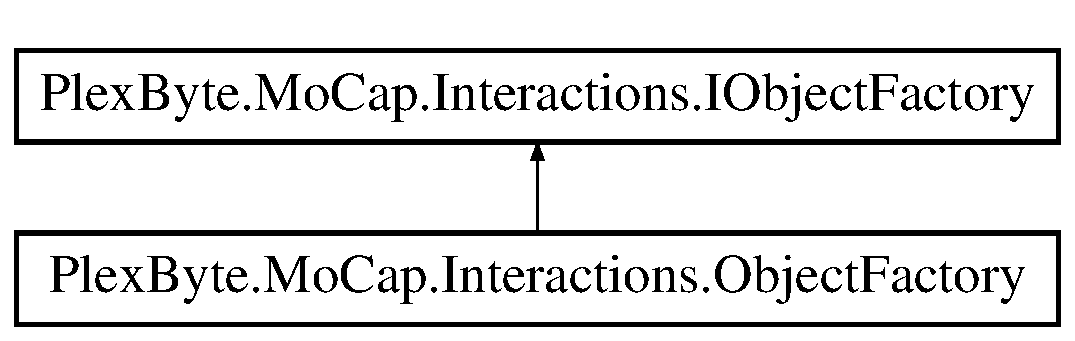
\includegraphics[height=2.000000cm]{interface_plex_byte_1_1_mo_cap_1_1_interactions_1_1_i_object_factory}
\end{center}
\end{figure}
\subsection*{Public Member Functions}
\begin{DoxyCompactItemize}
\item 
\hyperlink{interface_plex_byte_1_1_mo_cap_1_1_interactions_1_1_i_vote}{I\+Vote} \hyperlink{interface_plex_byte_1_1_mo_cap_1_1_interactions_1_1_i_object_factory_ab5ccd5e80e15d76d79504bfe4da715ca}{Create\+Vote} (string p\+Id, I\+User p\+User, \hyperlink{interface_plex_byte_1_1_mo_cap_1_1_interactions_1_1_i_survey_option}{I\+Survey\+Option} p\+Option)
\item 
\hyperlink{interface_plex_byte_1_1_mo_cap_1_1_interactions_1_1_i_survey_option}{I\+Survey\+Option} \hyperlink{interface_plex_byte_1_1_mo_cap_1_1_interactions_1_1_i_object_factory_ad181f2994305f53982828d0d3d8c4621}{Create\+Survey\+Option} (string p\+Id, string p\+Text)
\item 
I\+User \hyperlink{interface_plex_byte_1_1_mo_cap_1_1_interactions_1_1_i_object_factory_ab92eabebbc7307ae04940f46c88b2a30}{Create\+User} (string p\+Id, string p\+First\+Name, string p\+Last\+Name, string p\+Middle\+Name, string p\+Email, Date\+Time p\+Birthdate, string p\+User\+Name, string p\+Password, Date\+Time p\+Modified, Date\+Time p\+Created, string p\+Person\+Id)
\end{DoxyCompactItemize}


\subsection{Detailed Description}


Definition at line 12 of file I\+Object\+Factory.\+cs.



\subsection{Member Function Documentation}
\index{Plex\+Byte\+::\+Mo\+Cap\+::\+Interactions\+::\+I\+Object\+Factory@{Plex\+Byte\+::\+Mo\+Cap\+::\+Interactions\+::\+I\+Object\+Factory}!Create\+Survey\+Option@{Create\+Survey\+Option}}
\index{Create\+Survey\+Option@{Create\+Survey\+Option}!Plex\+Byte\+::\+Mo\+Cap\+::\+Interactions\+::\+I\+Object\+Factory@{Plex\+Byte\+::\+Mo\+Cap\+::\+Interactions\+::\+I\+Object\+Factory}}
\subsubsection[{\texorpdfstring{Create\+Survey\+Option(string p\+Id, string p\+Text)}{CreateSurveyOption(string pId, string pText)}}]{\setlength{\rightskip}{0pt plus 5cm}{\bf I\+Survey\+Option} Plex\+Byte.\+Mo\+Cap.\+Interactions.\+I\+Object\+Factory.\+Create\+Survey\+Option (
\begin{DoxyParamCaption}
\item[{string}]{p\+Id, }
\item[{string}]{p\+Text}
\end{DoxyParamCaption}
)}\hypertarget{interface_plex_byte_1_1_mo_cap_1_1_interactions_1_1_i_object_factory_ad181f2994305f53982828d0d3d8c4621}{}\label{interface_plex_byte_1_1_mo_cap_1_1_interactions_1_1_i_object_factory_ad181f2994305f53982828d0d3d8c4621}


Implemented in \hyperlink{class_plex_byte_1_1_mo_cap_1_1_interactions_1_1_object_factory_ad3a9a100069f91f229baa9bfe1a1205a}{Plex\+Byte.\+Mo\+Cap.\+Interactions.\+Object\+Factory}.

\index{Plex\+Byte\+::\+Mo\+Cap\+::\+Interactions\+::\+I\+Object\+Factory@{Plex\+Byte\+::\+Mo\+Cap\+::\+Interactions\+::\+I\+Object\+Factory}!Create\+User@{Create\+User}}
\index{Create\+User@{Create\+User}!Plex\+Byte\+::\+Mo\+Cap\+::\+Interactions\+::\+I\+Object\+Factory@{Plex\+Byte\+::\+Mo\+Cap\+::\+Interactions\+::\+I\+Object\+Factory}}
\subsubsection[{\texorpdfstring{Create\+User(string p\+Id, string p\+First\+Name, string p\+Last\+Name, string p\+Middle\+Name, string p\+Email, Date\+Time p\+Birthdate, string p\+User\+Name, string p\+Password, Date\+Time p\+Modified, Date\+Time p\+Created, string p\+Person\+Id)}{CreateUser(string pId, string pFirstName, string pLastName, string pMiddleName, string pEmail, DateTime pBirthdate, string pUserName, string pPassword, DateTime pModified, DateTime pCreated, string pPersonId)}}]{\setlength{\rightskip}{0pt plus 5cm}I\+User Plex\+Byte.\+Mo\+Cap.\+Interactions.\+I\+Object\+Factory.\+Create\+User (
\begin{DoxyParamCaption}
\item[{string}]{p\+Id, }
\item[{string}]{p\+First\+Name, }
\item[{string}]{p\+Last\+Name, }
\item[{string}]{p\+Middle\+Name, }
\item[{string}]{p\+Email, }
\item[{Date\+Time}]{p\+Birthdate, }
\item[{string}]{p\+User\+Name, }
\item[{string}]{p\+Password, }
\item[{Date\+Time}]{p\+Modified, }
\item[{Date\+Time}]{p\+Created, }
\item[{string}]{p\+Person\+Id}
\end{DoxyParamCaption}
)}\hypertarget{interface_plex_byte_1_1_mo_cap_1_1_interactions_1_1_i_object_factory_ab92eabebbc7307ae04940f46c88b2a30}{}\label{interface_plex_byte_1_1_mo_cap_1_1_interactions_1_1_i_object_factory_ab92eabebbc7307ae04940f46c88b2a30}


Implemented in \hyperlink{class_plex_byte_1_1_mo_cap_1_1_interactions_1_1_object_factory_add6cc462c161e617c99f76512fb359dd}{Plex\+Byte.\+Mo\+Cap.\+Interactions.\+Object\+Factory}.

\index{Plex\+Byte\+::\+Mo\+Cap\+::\+Interactions\+::\+I\+Object\+Factory@{Plex\+Byte\+::\+Mo\+Cap\+::\+Interactions\+::\+I\+Object\+Factory}!Create\+Vote@{Create\+Vote}}
\index{Create\+Vote@{Create\+Vote}!Plex\+Byte\+::\+Mo\+Cap\+::\+Interactions\+::\+I\+Object\+Factory@{Plex\+Byte\+::\+Mo\+Cap\+::\+Interactions\+::\+I\+Object\+Factory}}
\subsubsection[{\texorpdfstring{Create\+Vote(string p\+Id, I\+User p\+User, I\+Survey\+Option p\+Option)}{CreateVote(string pId, IUser pUser, ISurveyOption pOption)}}]{\setlength{\rightskip}{0pt plus 5cm}{\bf I\+Vote} Plex\+Byte.\+Mo\+Cap.\+Interactions.\+I\+Object\+Factory.\+Create\+Vote (
\begin{DoxyParamCaption}
\item[{string}]{p\+Id, }
\item[{I\+User}]{p\+User, }
\item[{{\bf I\+Survey\+Option}}]{p\+Option}
\end{DoxyParamCaption}
)}\hypertarget{interface_plex_byte_1_1_mo_cap_1_1_interactions_1_1_i_object_factory_ab5ccd5e80e15d76d79504bfe4da715ca}{}\label{interface_plex_byte_1_1_mo_cap_1_1_interactions_1_1_i_object_factory_ab5ccd5e80e15d76d79504bfe4da715ca}


Implemented in \hyperlink{class_plex_byte_1_1_mo_cap_1_1_interactions_1_1_object_factory_a5e26c538cb579f1a31798ce1ae6a4c2f}{Plex\+Byte.\+Mo\+Cap.\+Interactions.\+Object\+Factory}.



The documentation for this interface was generated from the following file\+:\begin{DoxyCompactItemize}
\item 
D\+:/\+Users/\+Christian\+B/\+Documents/\+\_\+\+H\+F Infomatik/\+Git\+Hub\+\_\+\+Repos/\+Mo\+Cap/\+Plex\+Byte.\+Mo\+Cap/\+Plex\+Byte.\+Mo\+Cap.\+Interactions/\hyperlink{_i_object_factory_8cs}{I\+Object\+Factory.\+cs}\end{DoxyCompactItemize}

\hypertarget{interface_plex_byte_1_1_mo_cap_1_1_interactions_1_1_i_project}{}\section{Plex\+Byte.\+Mo\+Cap.\+Interactions.\+I\+Project Interface Reference}
\label{interface_plex_byte_1_1_mo_cap_1_1_interactions_1_1_i_project}\index{Plex\+Byte.\+Mo\+Cap.\+Interactions.\+I\+Project@{Plex\+Byte.\+Mo\+Cap.\+Interactions.\+I\+Project}}
Inheritance diagram for Plex\+Byte.\+Mo\+Cap.\+Interactions.\+I\+Project\+:\begin{figure}[H]
\begin{center}
\leavevmode
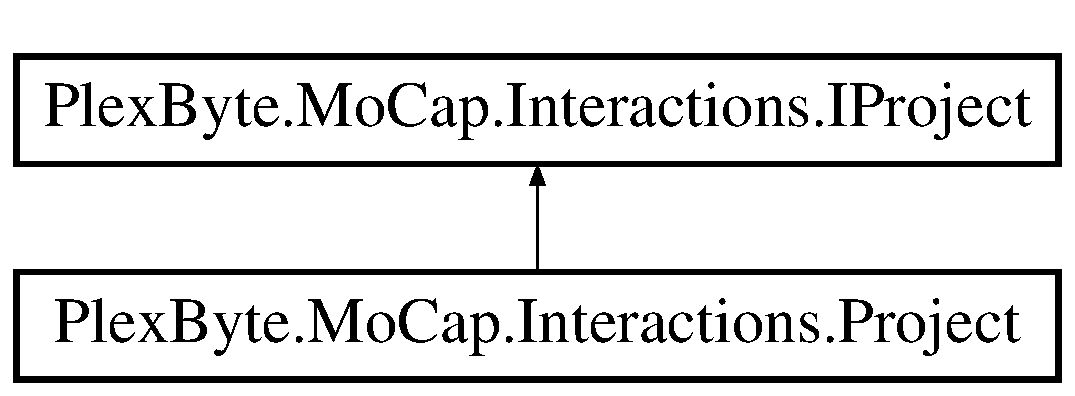
\includegraphics[height=2.000000cm]{interface_plex_byte_1_1_mo_cap_1_1_interactions_1_1_i_project}
\end{center}
\end{figure}
\subsection*{Public Member Functions}
\begin{DoxyCompactItemize}
\item 
void \hyperlink{interface_plex_byte_1_1_mo_cap_1_1_interactions_1_1_i_project_a9ce2ef4ee8b2d18da93405ea42113980}{Add\+Task} (\hyperlink{interface_plex_byte_1_1_mo_cap_1_1_interactions_1_1_i_task}{I\+Task} p\+Task)
\item 
void \hyperlink{interface_plex_byte_1_1_mo_cap_1_1_interactions_1_1_i_project_abd866426be16a3223f4930f6501e7114}{Add\+Survey} (\hyperlink{interface_plex_byte_1_1_mo_cap_1_1_interactions_1_1_i_survey}{I\+Survey} p\+Survey)
\item 
void \hyperlink{interface_plex_byte_1_1_mo_cap_1_1_interactions_1_1_i_project_a9ddad78d3c2f514d72f41cf9a6465956}{Invite} (I\+User p\+User)
\item 
void \hyperlink{interface_plex_byte_1_1_mo_cap_1_1_interactions_1_1_i_project_ab3bcc21a56e10b5e44381fe133420f71}{Accept} (I\+User p\+User)
\item 
void \hyperlink{interface_plex_byte_1_1_mo_cap_1_1_interactions_1_1_i_project_ad80e36a0f7acdba35550ebf57cbdda58}{Leave} (I\+User p\+User)
\item 
void \hyperlink{interface_plex_byte_1_1_mo_cap_1_1_interactions_1_1_i_project_a7c6e41fc59f57b0eba49a9e1a5d94d42}{Kick\+User} (I\+User p\+User)
\end{DoxyCompactItemize}
\subsection*{Properties}
\begin{DoxyCompactItemize}
\item 
string \hyperlink{interface_plex_byte_1_1_mo_cap_1_1_interactions_1_1_i_project_a95947061f781575e3df3bf6658cb86d0}{Id}\hspace{0.3cm}{\ttfamily  \mbox{[}get\mbox{]}}
\item 
Date\+Time \hyperlink{interface_plex_byte_1_1_mo_cap_1_1_interactions_1_1_i_project_af8868c724e9a25b74a30b85b4654956b}{Created\+Date\+Time}\hspace{0.3cm}{\ttfamily  \mbox{[}get\mbox{]}}
\item 
Date\+Time \hyperlink{interface_plex_byte_1_1_mo_cap_1_1_interactions_1_1_i_project_aee621c808ca4a5d55d494800eae4f6c3}{Modified\+Date\+Time}\hspace{0.3cm}{\ttfamily  \mbox{[}get\mbox{]}}
\item 
bool \hyperlink{interface_plex_byte_1_1_mo_cap_1_1_interactions_1_1_i_project_a28353591309223c5eb12360d6bdac936}{Enable\+Balance}\hspace{0.3cm}{\ttfamily  \mbox{[}get\mbox{]}}
\item 
I\+User \hyperlink{interface_plex_byte_1_1_mo_cap_1_1_interactions_1_1_i_project_a7ba31b458f048ceff4798085f742d5cd}{Creator}\hspace{0.3cm}{\ttfamily  \mbox{[}get\mbox{]}}
\item 
bool \hyperlink{interface_plex_byte_1_1_mo_cap_1_1_interactions_1_1_i_project_a80a6ab05af2dbe0046179fa69235a42e}{Enable\+Survey}\hspace{0.3cm}{\ttfamily  \mbox{[}get\mbox{]}}
\item 
List$<$ I\+User $>$ \hyperlink{interface_plex_byte_1_1_mo_cap_1_1_interactions_1_1_i_project_a377cc2be7bd29881bfc0b50a4a5e2cdd}{Invitation\+List}\hspace{0.3cm}{\ttfamily  \mbox{[}get\mbox{]}}
\item 
\hyperlink{interface_plex_byte_1_1_mo_cap_1_1_interactions_1_1_i_account}{I\+Account} \hyperlink{interface_plex_byte_1_1_mo_cap_1_1_interactions_1_1_i_project_a617958b9559bd24c0c6827e0827bd26f}{Project\+Account}\hspace{0.3cm}{\ttfamily  \mbox{[}get, set\mbox{]}}
\item 
List$<$ \hyperlink{interface_plex_byte_1_1_mo_cap_1_1_interactions_1_1_i_task}{I\+Task} $>$ \hyperlink{interface_plex_byte_1_1_mo_cap_1_1_interactions_1_1_i_project_a5c3f958126f3834f218b8b1302ef19a6}{Task\+List}\hspace{0.3cm}{\ttfamily  \mbox{[}get\mbox{]}}
\item 
List$<$ \hyperlink{interface_plex_byte_1_1_mo_cap_1_1_interactions_1_1_i_survey}{I\+Survey} $>$ \hyperlink{interface_plex_byte_1_1_mo_cap_1_1_interactions_1_1_i_project_a697de4384c6cf9e64a8242011da303c4}{Survey\+List}\hspace{0.3cm}{\ttfamily  \mbox{[}get\mbox{]}}
\item 
List$<$ I\+User $>$ \hyperlink{interface_plex_byte_1_1_mo_cap_1_1_interactions_1_1_i_project_afd9d799c7b5d0054ef537212bcead510}{Member\+List}\hspace{0.3cm}{\ttfamily  \mbox{[}get\mbox{]}}
\end{DoxyCompactItemize}
\subsection*{Events}
\begin{DoxyCompactItemize}
\item 
\hyperlink{namespace_plex_byte_1_1_mo_cap_1_1_interactions_aef92e5d1e9d0a246188e890e95317f08}{User\+Invite} \hyperlink{interface_plex_byte_1_1_mo_cap_1_1_interactions_1_1_i_project_abadab34acdb83e046e9ae803e22c2d27}{User\+Invited}
\item 
\hyperlink{namespace_plex_byte_1_1_mo_cap_1_1_interactions_a16841bb191709e7941fc1acb4d96f24f}{User\+Add} \hyperlink{interface_plex_byte_1_1_mo_cap_1_1_interactions_1_1_i_project_a5d5c412422011210e3a86243e25fb372}{User\+Added}
\item 
\hyperlink{namespace_plex_byte_1_1_mo_cap_1_1_interactions_a7dea125552945356069febe97eb72332}{User\+Ban} \hyperlink{interface_plex_byte_1_1_mo_cap_1_1_interactions_1_1_i_project_a8b16634c624d73da66c0c242f44ce711}{User\+Banned}
\item 
\hyperlink{interface_plex_byte_1_1_mo_cap_1_1_interactions_1_1_i_project_ad80e36a0f7acdba35550ebf57cbdda58}{Leave} \hyperlink{interface_plex_byte_1_1_mo_cap_1_1_interactions_1_1_i_project_a5e5266a4b705cbe91b27b6ddd0d63713}{Left}
\item 
\hyperlink{namespace_plex_byte_1_1_mo_cap_1_1_interactions_a15d0878ea4e4b99061b0424143eb2ce5}{Task\+Add} \hyperlink{interface_plex_byte_1_1_mo_cap_1_1_interactions_1_1_i_project_aedc4e43b2efa4b28fab73d4f620a7533}{Task\+Added}
\item 
\hyperlink{namespace_plex_byte_1_1_mo_cap_1_1_interactions_a1900501fc00150a42afd117937b7e88e}{Survey\+Add} \hyperlink{interface_plex_byte_1_1_mo_cap_1_1_interactions_1_1_i_project_a4c42760e1b0fc98b56bbd55c1df01ea5}{Survey\+Added}
\end{DoxyCompactItemize}


\subsection{Detailed Description}


Definition at line 19 of file I\+Project.\+cs.



\subsection{Member Function Documentation}
\index{Plex\+Byte\+::\+Mo\+Cap\+::\+Interactions\+::\+I\+Project@{Plex\+Byte\+::\+Mo\+Cap\+::\+Interactions\+::\+I\+Project}!Accept@{Accept}}
\index{Accept@{Accept}!Plex\+Byte\+::\+Mo\+Cap\+::\+Interactions\+::\+I\+Project@{Plex\+Byte\+::\+Mo\+Cap\+::\+Interactions\+::\+I\+Project}}
\subsubsection[{\texorpdfstring{Accept(\+I\+User p\+User)}{Accept(IUser pUser)}}]{\setlength{\rightskip}{0pt plus 5cm}void Plex\+Byte.\+Mo\+Cap.\+Interactions.\+I\+Project.\+Accept (
\begin{DoxyParamCaption}
\item[{I\+User}]{p\+User}
\end{DoxyParamCaption}
)}\hypertarget{interface_plex_byte_1_1_mo_cap_1_1_interactions_1_1_i_project_ab3bcc21a56e10b5e44381fe133420f71}{}\label{interface_plex_byte_1_1_mo_cap_1_1_interactions_1_1_i_project_ab3bcc21a56e10b5e44381fe133420f71}


Implemented in \hyperlink{class_plex_byte_1_1_mo_cap_1_1_interactions_1_1_project_a06b884b97b543b4c8ba64993e4008a6f}{Plex\+Byte.\+Mo\+Cap.\+Interactions.\+Project}.

\index{Plex\+Byte\+::\+Mo\+Cap\+::\+Interactions\+::\+I\+Project@{Plex\+Byte\+::\+Mo\+Cap\+::\+Interactions\+::\+I\+Project}!Add\+Survey@{Add\+Survey}}
\index{Add\+Survey@{Add\+Survey}!Plex\+Byte\+::\+Mo\+Cap\+::\+Interactions\+::\+I\+Project@{Plex\+Byte\+::\+Mo\+Cap\+::\+Interactions\+::\+I\+Project}}
\subsubsection[{\texorpdfstring{Add\+Survey(\+I\+Survey p\+Survey)}{AddSurvey(ISurvey pSurvey)}}]{\setlength{\rightskip}{0pt plus 5cm}void Plex\+Byte.\+Mo\+Cap.\+Interactions.\+I\+Project.\+Add\+Survey (
\begin{DoxyParamCaption}
\item[{{\bf I\+Survey}}]{p\+Survey}
\end{DoxyParamCaption}
)}\hypertarget{interface_plex_byte_1_1_mo_cap_1_1_interactions_1_1_i_project_abd866426be16a3223f4930f6501e7114}{}\label{interface_plex_byte_1_1_mo_cap_1_1_interactions_1_1_i_project_abd866426be16a3223f4930f6501e7114}


Implemented in \hyperlink{class_plex_byte_1_1_mo_cap_1_1_interactions_1_1_project_af374761c89f59d42b1a79fdb5cf0311d}{Plex\+Byte.\+Mo\+Cap.\+Interactions.\+Project}.

\index{Plex\+Byte\+::\+Mo\+Cap\+::\+Interactions\+::\+I\+Project@{Plex\+Byte\+::\+Mo\+Cap\+::\+Interactions\+::\+I\+Project}!Add\+Task@{Add\+Task}}
\index{Add\+Task@{Add\+Task}!Plex\+Byte\+::\+Mo\+Cap\+::\+Interactions\+::\+I\+Project@{Plex\+Byte\+::\+Mo\+Cap\+::\+Interactions\+::\+I\+Project}}
\subsubsection[{\texorpdfstring{Add\+Task(\+I\+Task p\+Task)}{AddTask(ITask pTask)}}]{\setlength{\rightskip}{0pt plus 5cm}void Plex\+Byte.\+Mo\+Cap.\+Interactions.\+I\+Project.\+Add\+Task (
\begin{DoxyParamCaption}
\item[{{\bf I\+Task}}]{p\+Task}
\end{DoxyParamCaption}
)}\hypertarget{interface_plex_byte_1_1_mo_cap_1_1_interactions_1_1_i_project_a9ce2ef4ee8b2d18da93405ea42113980}{}\label{interface_plex_byte_1_1_mo_cap_1_1_interactions_1_1_i_project_a9ce2ef4ee8b2d18da93405ea42113980}


Implemented in \hyperlink{class_plex_byte_1_1_mo_cap_1_1_interactions_1_1_project_a4d3d0c6c63e3dc3162ec2f5a314bade1}{Plex\+Byte.\+Mo\+Cap.\+Interactions.\+Project}.

\index{Plex\+Byte\+::\+Mo\+Cap\+::\+Interactions\+::\+I\+Project@{Plex\+Byte\+::\+Mo\+Cap\+::\+Interactions\+::\+I\+Project}!Invite@{Invite}}
\index{Invite@{Invite}!Plex\+Byte\+::\+Mo\+Cap\+::\+Interactions\+::\+I\+Project@{Plex\+Byte\+::\+Mo\+Cap\+::\+Interactions\+::\+I\+Project}}
\subsubsection[{\texorpdfstring{Invite(\+I\+User p\+User)}{Invite(IUser pUser)}}]{\setlength{\rightskip}{0pt plus 5cm}void Plex\+Byte.\+Mo\+Cap.\+Interactions.\+I\+Project.\+Invite (
\begin{DoxyParamCaption}
\item[{I\+User}]{p\+User}
\end{DoxyParamCaption}
)}\hypertarget{interface_plex_byte_1_1_mo_cap_1_1_interactions_1_1_i_project_a9ddad78d3c2f514d72f41cf9a6465956}{}\label{interface_plex_byte_1_1_mo_cap_1_1_interactions_1_1_i_project_a9ddad78d3c2f514d72f41cf9a6465956}


Implemented in \hyperlink{class_plex_byte_1_1_mo_cap_1_1_interactions_1_1_project_a44b3e36d693cffce67d606f2f040927e}{Plex\+Byte.\+Mo\+Cap.\+Interactions.\+Project}.

\index{Plex\+Byte\+::\+Mo\+Cap\+::\+Interactions\+::\+I\+Project@{Plex\+Byte\+::\+Mo\+Cap\+::\+Interactions\+::\+I\+Project}!Kick\+User@{Kick\+User}}
\index{Kick\+User@{Kick\+User}!Plex\+Byte\+::\+Mo\+Cap\+::\+Interactions\+::\+I\+Project@{Plex\+Byte\+::\+Mo\+Cap\+::\+Interactions\+::\+I\+Project}}
\subsubsection[{\texorpdfstring{Kick\+User(\+I\+User p\+User)}{KickUser(IUser pUser)}}]{\setlength{\rightskip}{0pt plus 5cm}void Plex\+Byte.\+Mo\+Cap.\+Interactions.\+I\+Project.\+Kick\+User (
\begin{DoxyParamCaption}
\item[{I\+User}]{p\+User}
\end{DoxyParamCaption}
)}\hypertarget{interface_plex_byte_1_1_mo_cap_1_1_interactions_1_1_i_project_a7c6e41fc59f57b0eba49a9e1a5d94d42}{}\label{interface_plex_byte_1_1_mo_cap_1_1_interactions_1_1_i_project_a7c6e41fc59f57b0eba49a9e1a5d94d42}


Implemented in \hyperlink{class_plex_byte_1_1_mo_cap_1_1_interactions_1_1_project_a0fe352bded53612ae6e23859b0ce8802}{Plex\+Byte.\+Mo\+Cap.\+Interactions.\+Project}.

\index{Plex\+Byte\+::\+Mo\+Cap\+::\+Interactions\+::\+I\+Project@{Plex\+Byte\+::\+Mo\+Cap\+::\+Interactions\+::\+I\+Project}!Leave@{Leave}}
\index{Leave@{Leave}!Plex\+Byte\+::\+Mo\+Cap\+::\+Interactions\+::\+I\+Project@{Plex\+Byte\+::\+Mo\+Cap\+::\+Interactions\+::\+I\+Project}}
\subsubsection[{\texorpdfstring{Leave(\+I\+User p\+User)}{Leave(IUser pUser)}}]{\setlength{\rightskip}{0pt plus 5cm}void Plex\+Byte.\+Mo\+Cap.\+Interactions.\+I\+Project.\+Leave (
\begin{DoxyParamCaption}
\item[{I\+User}]{p\+User}
\end{DoxyParamCaption}
)}\hypertarget{interface_plex_byte_1_1_mo_cap_1_1_interactions_1_1_i_project_ad80e36a0f7acdba35550ebf57cbdda58}{}\label{interface_plex_byte_1_1_mo_cap_1_1_interactions_1_1_i_project_ad80e36a0f7acdba35550ebf57cbdda58}


Implemented in \hyperlink{class_plex_byte_1_1_mo_cap_1_1_interactions_1_1_project_a12152d11fc38eedc1b93dd56ee73f42c}{Plex\+Byte.\+Mo\+Cap.\+Interactions.\+Project}.



\subsection{Property Documentation}
\index{Plex\+Byte\+::\+Mo\+Cap\+::\+Interactions\+::\+I\+Project@{Plex\+Byte\+::\+Mo\+Cap\+::\+Interactions\+::\+I\+Project}!Created\+Date\+Time@{Created\+Date\+Time}}
\index{Created\+Date\+Time@{Created\+Date\+Time}!Plex\+Byte\+::\+Mo\+Cap\+::\+Interactions\+::\+I\+Project@{Plex\+Byte\+::\+Mo\+Cap\+::\+Interactions\+::\+I\+Project}}
\subsubsection[{\texorpdfstring{Created\+Date\+Time}{CreatedDateTime}}]{\setlength{\rightskip}{0pt plus 5cm}Date\+Time Plex\+Byte.\+Mo\+Cap.\+Interactions.\+I\+Project.\+Created\+Date\+Time\hspace{0.3cm}{\ttfamily [get]}}\hypertarget{interface_plex_byte_1_1_mo_cap_1_1_interactions_1_1_i_project_af8868c724e9a25b74a30b85b4654956b}{}\label{interface_plex_byte_1_1_mo_cap_1_1_interactions_1_1_i_project_af8868c724e9a25b74a30b85b4654956b}


Definition at line 32 of file I\+Project.\+cs.

\index{Plex\+Byte\+::\+Mo\+Cap\+::\+Interactions\+::\+I\+Project@{Plex\+Byte\+::\+Mo\+Cap\+::\+Interactions\+::\+I\+Project}!Creator@{Creator}}
\index{Creator@{Creator}!Plex\+Byte\+::\+Mo\+Cap\+::\+Interactions\+::\+I\+Project@{Plex\+Byte\+::\+Mo\+Cap\+::\+Interactions\+::\+I\+Project}}
\subsubsection[{\texorpdfstring{Creator}{Creator}}]{\setlength{\rightskip}{0pt plus 5cm}I\+User Plex\+Byte.\+Mo\+Cap.\+Interactions.\+I\+Project.\+Creator\hspace{0.3cm}{\ttfamily [get]}}\hypertarget{interface_plex_byte_1_1_mo_cap_1_1_interactions_1_1_i_project_a7ba31b458f048ceff4798085f742d5cd}{}\label{interface_plex_byte_1_1_mo_cap_1_1_interactions_1_1_i_project_a7ba31b458f048ceff4798085f742d5cd}


Definition at line 38 of file I\+Project.\+cs.

\index{Plex\+Byte\+::\+Mo\+Cap\+::\+Interactions\+::\+I\+Project@{Plex\+Byte\+::\+Mo\+Cap\+::\+Interactions\+::\+I\+Project}!Enable\+Balance@{Enable\+Balance}}
\index{Enable\+Balance@{Enable\+Balance}!Plex\+Byte\+::\+Mo\+Cap\+::\+Interactions\+::\+I\+Project@{Plex\+Byte\+::\+Mo\+Cap\+::\+Interactions\+::\+I\+Project}}
\subsubsection[{\texorpdfstring{Enable\+Balance}{EnableBalance}}]{\setlength{\rightskip}{0pt plus 5cm}bool Plex\+Byte.\+Mo\+Cap.\+Interactions.\+I\+Project.\+Enable\+Balance\hspace{0.3cm}{\ttfamily [get]}}\hypertarget{interface_plex_byte_1_1_mo_cap_1_1_interactions_1_1_i_project_a28353591309223c5eb12360d6bdac936}{}\label{interface_plex_byte_1_1_mo_cap_1_1_interactions_1_1_i_project_a28353591309223c5eb12360d6bdac936}


Definition at line 36 of file I\+Project.\+cs.

\index{Plex\+Byte\+::\+Mo\+Cap\+::\+Interactions\+::\+I\+Project@{Plex\+Byte\+::\+Mo\+Cap\+::\+Interactions\+::\+I\+Project}!Enable\+Survey@{Enable\+Survey}}
\index{Enable\+Survey@{Enable\+Survey}!Plex\+Byte\+::\+Mo\+Cap\+::\+Interactions\+::\+I\+Project@{Plex\+Byte\+::\+Mo\+Cap\+::\+Interactions\+::\+I\+Project}}
\subsubsection[{\texorpdfstring{Enable\+Survey}{EnableSurvey}}]{\setlength{\rightskip}{0pt plus 5cm}bool Plex\+Byte.\+Mo\+Cap.\+Interactions.\+I\+Project.\+Enable\+Survey\hspace{0.3cm}{\ttfamily [get]}}\hypertarget{interface_plex_byte_1_1_mo_cap_1_1_interactions_1_1_i_project_a80a6ab05af2dbe0046179fa69235a42e}{}\label{interface_plex_byte_1_1_mo_cap_1_1_interactions_1_1_i_project_a80a6ab05af2dbe0046179fa69235a42e}


Definition at line 40 of file I\+Project.\+cs.

\index{Plex\+Byte\+::\+Mo\+Cap\+::\+Interactions\+::\+I\+Project@{Plex\+Byte\+::\+Mo\+Cap\+::\+Interactions\+::\+I\+Project}!Id@{Id}}
\index{Id@{Id}!Plex\+Byte\+::\+Mo\+Cap\+::\+Interactions\+::\+I\+Project@{Plex\+Byte\+::\+Mo\+Cap\+::\+Interactions\+::\+I\+Project}}
\subsubsection[{\texorpdfstring{Id}{Id}}]{\setlength{\rightskip}{0pt plus 5cm}string Plex\+Byte.\+Mo\+Cap.\+Interactions.\+I\+Project.\+Id\hspace{0.3cm}{\ttfamily [get]}}\hypertarget{interface_plex_byte_1_1_mo_cap_1_1_interactions_1_1_i_project_a95947061f781575e3df3bf6658cb86d0}{}\label{interface_plex_byte_1_1_mo_cap_1_1_interactions_1_1_i_project_a95947061f781575e3df3bf6658cb86d0}


Definition at line 30 of file I\+Project.\+cs.

\index{Plex\+Byte\+::\+Mo\+Cap\+::\+Interactions\+::\+I\+Project@{Plex\+Byte\+::\+Mo\+Cap\+::\+Interactions\+::\+I\+Project}!Invitation\+List@{Invitation\+List}}
\index{Invitation\+List@{Invitation\+List}!Plex\+Byte\+::\+Mo\+Cap\+::\+Interactions\+::\+I\+Project@{Plex\+Byte\+::\+Mo\+Cap\+::\+Interactions\+::\+I\+Project}}
\subsubsection[{\texorpdfstring{Invitation\+List}{InvitationList}}]{\setlength{\rightskip}{0pt plus 5cm}List$<$I\+User$>$ Plex\+Byte.\+Mo\+Cap.\+Interactions.\+I\+Project.\+Invitation\+List\hspace{0.3cm}{\ttfamily [get]}}\hypertarget{interface_plex_byte_1_1_mo_cap_1_1_interactions_1_1_i_project_a377cc2be7bd29881bfc0b50a4a5e2cdd}{}\label{interface_plex_byte_1_1_mo_cap_1_1_interactions_1_1_i_project_a377cc2be7bd29881bfc0b50a4a5e2cdd}


Definition at line 42 of file I\+Project.\+cs.

\index{Plex\+Byte\+::\+Mo\+Cap\+::\+Interactions\+::\+I\+Project@{Plex\+Byte\+::\+Mo\+Cap\+::\+Interactions\+::\+I\+Project}!Member\+List@{Member\+List}}
\index{Member\+List@{Member\+List}!Plex\+Byte\+::\+Mo\+Cap\+::\+Interactions\+::\+I\+Project@{Plex\+Byte\+::\+Mo\+Cap\+::\+Interactions\+::\+I\+Project}}
\subsubsection[{\texorpdfstring{Member\+List}{MemberList}}]{\setlength{\rightskip}{0pt plus 5cm}List$<$I\+User$>$ Plex\+Byte.\+Mo\+Cap.\+Interactions.\+I\+Project.\+Member\+List\hspace{0.3cm}{\ttfamily [get]}}\hypertarget{interface_plex_byte_1_1_mo_cap_1_1_interactions_1_1_i_project_afd9d799c7b5d0054ef537212bcead510}{}\label{interface_plex_byte_1_1_mo_cap_1_1_interactions_1_1_i_project_afd9d799c7b5d0054ef537212bcead510}


Definition at line 50 of file I\+Project.\+cs.

\index{Plex\+Byte\+::\+Mo\+Cap\+::\+Interactions\+::\+I\+Project@{Plex\+Byte\+::\+Mo\+Cap\+::\+Interactions\+::\+I\+Project}!Modified\+Date\+Time@{Modified\+Date\+Time}}
\index{Modified\+Date\+Time@{Modified\+Date\+Time}!Plex\+Byte\+::\+Mo\+Cap\+::\+Interactions\+::\+I\+Project@{Plex\+Byte\+::\+Mo\+Cap\+::\+Interactions\+::\+I\+Project}}
\subsubsection[{\texorpdfstring{Modified\+Date\+Time}{ModifiedDateTime}}]{\setlength{\rightskip}{0pt plus 5cm}Date\+Time Plex\+Byte.\+Mo\+Cap.\+Interactions.\+I\+Project.\+Modified\+Date\+Time\hspace{0.3cm}{\ttfamily [get]}}\hypertarget{interface_plex_byte_1_1_mo_cap_1_1_interactions_1_1_i_project_aee621c808ca4a5d55d494800eae4f6c3}{}\label{interface_plex_byte_1_1_mo_cap_1_1_interactions_1_1_i_project_aee621c808ca4a5d55d494800eae4f6c3}


Definition at line 34 of file I\+Project.\+cs.

\index{Plex\+Byte\+::\+Mo\+Cap\+::\+Interactions\+::\+I\+Project@{Plex\+Byte\+::\+Mo\+Cap\+::\+Interactions\+::\+I\+Project}!Project\+Account@{Project\+Account}}
\index{Project\+Account@{Project\+Account}!Plex\+Byte\+::\+Mo\+Cap\+::\+Interactions\+::\+I\+Project@{Plex\+Byte\+::\+Mo\+Cap\+::\+Interactions\+::\+I\+Project}}
\subsubsection[{\texorpdfstring{Project\+Account}{ProjectAccount}}]{\setlength{\rightskip}{0pt plus 5cm}{\bf I\+Account} Plex\+Byte.\+Mo\+Cap.\+Interactions.\+I\+Project.\+Project\+Account\hspace{0.3cm}{\ttfamily [get]}, {\ttfamily [set]}}\hypertarget{interface_plex_byte_1_1_mo_cap_1_1_interactions_1_1_i_project_a617958b9559bd24c0c6827e0827bd26f}{}\label{interface_plex_byte_1_1_mo_cap_1_1_interactions_1_1_i_project_a617958b9559bd24c0c6827e0827bd26f}


Definition at line 44 of file I\+Project.\+cs.

\index{Plex\+Byte\+::\+Mo\+Cap\+::\+Interactions\+::\+I\+Project@{Plex\+Byte\+::\+Mo\+Cap\+::\+Interactions\+::\+I\+Project}!Survey\+List@{Survey\+List}}
\index{Survey\+List@{Survey\+List}!Plex\+Byte\+::\+Mo\+Cap\+::\+Interactions\+::\+I\+Project@{Plex\+Byte\+::\+Mo\+Cap\+::\+Interactions\+::\+I\+Project}}
\subsubsection[{\texorpdfstring{Survey\+List}{SurveyList}}]{\setlength{\rightskip}{0pt plus 5cm}List$<${\bf I\+Survey}$>$ Plex\+Byte.\+Mo\+Cap.\+Interactions.\+I\+Project.\+Survey\+List\hspace{0.3cm}{\ttfamily [get]}}\hypertarget{interface_plex_byte_1_1_mo_cap_1_1_interactions_1_1_i_project_a697de4384c6cf9e64a8242011da303c4}{}\label{interface_plex_byte_1_1_mo_cap_1_1_interactions_1_1_i_project_a697de4384c6cf9e64a8242011da303c4}


Definition at line 48 of file I\+Project.\+cs.

\index{Plex\+Byte\+::\+Mo\+Cap\+::\+Interactions\+::\+I\+Project@{Plex\+Byte\+::\+Mo\+Cap\+::\+Interactions\+::\+I\+Project}!Task\+List@{Task\+List}}
\index{Task\+List@{Task\+List}!Plex\+Byte\+::\+Mo\+Cap\+::\+Interactions\+::\+I\+Project@{Plex\+Byte\+::\+Mo\+Cap\+::\+Interactions\+::\+I\+Project}}
\subsubsection[{\texorpdfstring{Task\+List}{TaskList}}]{\setlength{\rightskip}{0pt plus 5cm}List$<${\bf I\+Task}$>$ Plex\+Byte.\+Mo\+Cap.\+Interactions.\+I\+Project.\+Task\+List\hspace{0.3cm}{\ttfamily [get]}}\hypertarget{interface_plex_byte_1_1_mo_cap_1_1_interactions_1_1_i_project_a5c3f958126f3834f218b8b1302ef19a6}{}\label{interface_plex_byte_1_1_mo_cap_1_1_interactions_1_1_i_project_a5c3f958126f3834f218b8b1302ef19a6}


Definition at line 46 of file I\+Project.\+cs.



\subsection{Event Documentation}
\index{Plex\+Byte\+::\+Mo\+Cap\+::\+Interactions\+::\+I\+Project@{Plex\+Byte\+::\+Mo\+Cap\+::\+Interactions\+::\+I\+Project}!Left@{Left}}
\index{Left@{Left}!Plex\+Byte\+::\+Mo\+Cap\+::\+Interactions\+::\+I\+Project@{Plex\+Byte\+::\+Mo\+Cap\+::\+Interactions\+::\+I\+Project}}
\subsubsection[{\texorpdfstring{Left}{Left}}]{\setlength{\rightskip}{0pt plus 5cm}{\bf Leave} Plex\+Byte.\+Mo\+Cap.\+Interactions.\+I\+Project.\+Left}\hypertarget{interface_plex_byte_1_1_mo_cap_1_1_interactions_1_1_i_project_a5e5266a4b705cbe91b27b6ddd0d63713}{}\label{interface_plex_byte_1_1_mo_cap_1_1_interactions_1_1_i_project_a5e5266a4b705cbe91b27b6ddd0d63713}


Definition at line 25 of file I\+Project.\+cs.

\index{Plex\+Byte\+::\+Mo\+Cap\+::\+Interactions\+::\+I\+Project@{Plex\+Byte\+::\+Mo\+Cap\+::\+Interactions\+::\+I\+Project}!Survey\+Added@{Survey\+Added}}
\index{Survey\+Added@{Survey\+Added}!Plex\+Byte\+::\+Mo\+Cap\+::\+Interactions\+::\+I\+Project@{Plex\+Byte\+::\+Mo\+Cap\+::\+Interactions\+::\+I\+Project}}
\subsubsection[{\texorpdfstring{Survey\+Added}{SurveyAdded}}]{\setlength{\rightskip}{0pt plus 5cm}{\bf Survey\+Add} Plex\+Byte.\+Mo\+Cap.\+Interactions.\+I\+Project.\+Survey\+Added}\hypertarget{interface_plex_byte_1_1_mo_cap_1_1_interactions_1_1_i_project_a4c42760e1b0fc98b56bbd55c1df01ea5}{}\label{interface_plex_byte_1_1_mo_cap_1_1_interactions_1_1_i_project_a4c42760e1b0fc98b56bbd55c1df01ea5}


Definition at line 27 of file I\+Project.\+cs.

\index{Plex\+Byte\+::\+Mo\+Cap\+::\+Interactions\+::\+I\+Project@{Plex\+Byte\+::\+Mo\+Cap\+::\+Interactions\+::\+I\+Project}!Task\+Added@{Task\+Added}}
\index{Task\+Added@{Task\+Added}!Plex\+Byte\+::\+Mo\+Cap\+::\+Interactions\+::\+I\+Project@{Plex\+Byte\+::\+Mo\+Cap\+::\+Interactions\+::\+I\+Project}}
\subsubsection[{\texorpdfstring{Task\+Added}{TaskAdded}}]{\setlength{\rightskip}{0pt plus 5cm}{\bf Task\+Add} Plex\+Byte.\+Mo\+Cap.\+Interactions.\+I\+Project.\+Task\+Added}\hypertarget{interface_plex_byte_1_1_mo_cap_1_1_interactions_1_1_i_project_aedc4e43b2efa4b28fab73d4f620a7533}{}\label{interface_plex_byte_1_1_mo_cap_1_1_interactions_1_1_i_project_aedc4e43b2efa4b28fab73d4f620a7533}


Definition at line 26 of file I\+Project.\+cs.

\index{Plex\+Byte\+::\+Mo\+Cap\+::\+Interactions\+::\+I\+Project@{Plex\+Byte\+::\+Mo\+Cap\+::\+Interactions\+::\+I\+Project}!User\+Added@{User\+Added}}
\index{User\+Added@{User\+Added}!Plex\+Byte\+::\+Mo\+Cap\+::\+Interactions\+::\+I\+Project@{Plex\+Byte\+::\+Mo\+Cap\+::\+Interactions\+::\+I\+Project}}
\subsubsection[{\texorpdfstring{User\+Added}{UserAdded}}]{\setlength{\rightskip}{0pt plus 5cm}{\bf User\+Add} Plex\+Byte.\+Mo\+Cap.\+Interactions.\+I\+Project.\+User\+Added}\hypertarget{interface_plex_byte_1_1_mo_cap_1_1_interactions_1_1_i_project_a5d5c412422011210e3a86243e25fb372}{}\label{interface_plex_byte_1_1_mo_cap_1_1_interactions_1_1_i_project_a5d5c412422011210e3a86243e25fb372}


Definition at line 23 of file I\+Project.\+cs.

\index{Plex\+Byte\+::\+Mo\+Cap\+::\+Interactions\+::\+I\+Project@{Plex\+Byte\+::\+Mo\+Cap\+::\+Interactions\+::\+I\+Project}!User\+Banned@{User\+Banned}}
\index{User\+Banned@{User\+Banned}!Plex\+Byte\+::\+Mo\+Cap\+::\+Interactions\+::\+I\+Project@{Plex\+Byte\+::\+Mo\+Cap\+::\+Interactions\+::\+I\+Project}}
\subsubsection[{\texorpdfstring{User\+Banned}{UserBanned}}]{\setlength{\rightskip}{0pt plus 5cm}{\bf User\+Ban} Plex\+Byte.\+Mo\+Cap.\+Interactions.\+I\+Project.\+User\+Banned}\hypertarget{interface_plex_byte_1_1_mo_cap_1_1_interactions_1_1_i_project_a8b16634c624d73da66c0c242f44ce711}{}\label{interface_plex_byte_1_1_mo_cap_1_1_interactions_1_1_i_project_a8b16634c624d73da66c0c242f44ce711}


Definition at line 24 of file I\+Project.\+cs.

\index{Plex\+Byte\+::\+Mo\+Cap\+::\+Interactions\+::\+I\+Project@{Plex\+Byte\+::\+Mo\+Cap\+::\+Interactions\+::\+I\+Project}!User\+Invited@{User\+Invited}}
\index{User\+Invited@{User\+Invited}!Plex\+Byte\+::\+Mo\+Cap\+::\+Interactions\+::\+I\+Project@{Plex\+Byte\+::\+Mo\+Cap\+::\+Interactions\+::\+I\+Project}}
\subsubsection[{\texorpdfstring{User\+Invited}{UserInvited}}]{\setlength{\rightskip}{0pt plus 5cm}{\bf User\+Invite} Plex\+Byte.\+Mo\+Cap.\+Interactions.\+I\+Project.\+User\+Invited}\hypertarget{interface_plex_byte_1_1_mo_cap_1_1_interactions_1_1_i_project_abadab34acdb83e046e9ae803e22c2d27}{}\label{interface_plex_byte_1_1_mo_cap_1_1_interactions_1_1_i_project_abadab34acdb83e046e9ae803e22c2d27}


Definition at line 22 of file I\+Project.\+cs.



The documentation for this interface was generated from the following file\+:\begin{DoxyCompactItemize}
\item 
D\+:/\+Users/\+Christian\+B/\+Documents/\+\_\+\+H\+F Infomatik/\+Git\+Hub\+\_\+\+Repos/\+Mo\+Cap/\+Plex\+Byte.\+Mo\+Cap/\+Plex\+Byte.\+Mo\+Cap.\+Interactions/\hyperlink{_i_project_8cs}{I\+Project.\+cs}\end{DoxyCompactItemize}

\hypertarget{interface_plex_byte_1_1_mo_cap_1_1_interactions_1_1_i_survey}{}\section{Plex\+Byte.\+Mo\+Cap.\+Interactions.\+I\+Survey Interface Reference}
\label{interface_plex_byte_1_1_mo_cap_1_1_interactions_1_1_i_survey}\index{Plex\+Byte.\+Mo\+Cap.\+Interactions.\+I\+Survey@{Plex\+Byte.\+Mo\+Cap.\+Interactions.\+I\+Survey}}
Inheritance diagram for Plex\+Byte.\+Mo\+Cap.\+Interactions.\+I\+Survey\+:\begin{figure}[H]
\begin{center}
\leavevmode
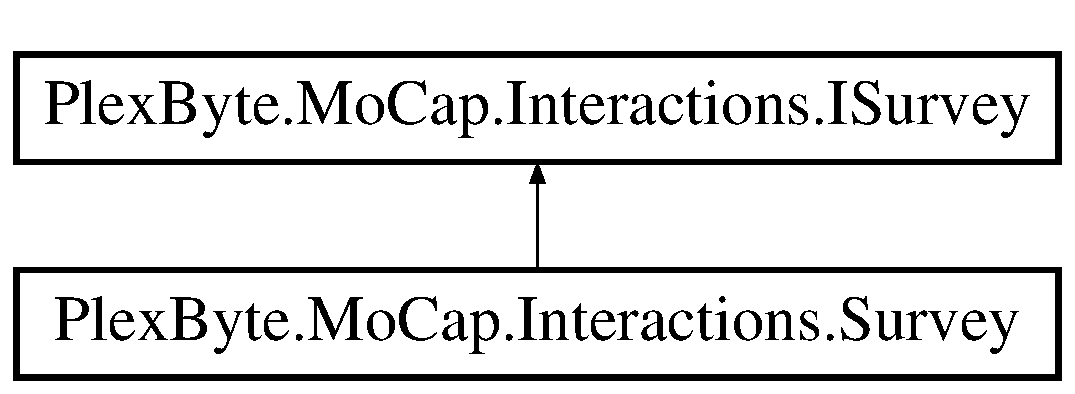
\includegraphics[height=2.000000cm]{interface_plex_byte_1_1_mo_cap_1_1_interactions_1_1_i_survey}
\end{center}
\end{figure}
\subsection*{Public Member Functions}
\begin{DoxyCompactItemize}
\item 
void \hyperlink{interface_plex_byte_1_1_mo_cap_1_1_interactions_1_1_i_survey_ab9df3eb58a1c66b14412cd1bd26f038c}{Add\+Vote} (\hyperlink{interface_plex_byte_1_1_mo_cap_1_1_interactions_1_1_i_vote}{I\+Vote} p\+Vote)
\item 
void \hyperlink{interface_plex_byte_1_1_mo_cap_1_1_interactions_1_1_i_survey_a19e6f79d6fc9ba6c8947894a0ab0d811}{Add\+Option} (\hyperlink{interface_plex_byte_1_1_mo_cap_1_1_interactions_1_1_i_survey_option}{I\+Survey\+Option} p\+Option)
\item 
void \hyperlink{interface_plex_byte_1_1_mo_cap_1_1_interactions_1_1_i_survey_a252050839e9167b57648e150a65385ea}{Add\+User} (I\+User p\+User)
\item 
void \hyperlink{interface_plex_byte_1_1_mo_cap_1_1_interactions_1_1_i_survey_a0e4b923ee86fb5031f0eaa9e3c81dbbd}{Remove\+User} (I\+User p\+User)
\end{DoxyCompactItemize}
\subsection*{Properties}
\begin{DoxyCompactItemize}
\item 
string \hyperlink{interface_plex_byte_1_1_mo_cap_1_1_interactions_1_1_i_survey_ad3a9fd1847c33d3204fa274ace8b9846}{Interaction\+Id}\hspace{0.3cm}{\ttfamily  \mbox{[}get, set\mbox{]}}
\item 
string \hyperlink{interface_plex_byte_1_1_mo_cap_1_1_interactions_1_1_i_survey_a6fb9f2c7bae0aa503035393f1af6b3b2}{Id}\hspace{0.3cm}{\ttfamily  \mbox{[}get, set\mbox{]}}
\item 
string \hyperlink{interface_plex_byte_1_1_mo_cap_1_1_interactions_1_1_i_survey_a883f1354055ab9ee92c915b0c80e4f09}{Project\+Id}\hspace{0.3cm}{\ttfamily  \mbox{[}get, set\mbox{]}}
\item 
string \hyperlink{interface_plex_byte_1_1_mo_cap_1_1_interactions_1_1_i_survey_ae7b5e153360d5d3ecba8c2d7a6f12bf4}{Title}\hspace{0.3cm}{\ttfamily  \mbox{[}get, set\mbox{]}}
\item 
Date\+Time \hyperlink{interface_plex_byte_1_1_mo_cap_1_1_interactions_1_1_i_survey_a1889aa237e8b5f47ac9efe0aece8e574}{Due\+Date\+Time}\hspace{0.3cm}{\ttfamily  \mbox{[}get, set\mbox{]}}
\item 
List$<$ \hyperlink{interface_plex_byte_1_1_mo_cap_1_1_interactions_1_1_i_survey_option}{I\+Survey\+Option} $>$ \hyperlink{interface_plex_byte_1_1_mo_cap_1_1_interactions_1_1_i_survey_aa346d9b90290f6d4871624d8ed2b848b}{Option\+List}\hspace{0.3cm}{\ttfamily  \mbox{[}get, set\mbox{]}}
\item 
List$<$ \hyperlink{interface_plex_byte_1_1_mo_cap_1_1_interactions_1_1_i_vote}{I\+Vote} $>$ \hyperlink{interface_plex_byte_1_1_mo_cap_1_1_interactions_1_1_i_survey_a86a110a0d3506ced724e5246fb3596ad}{Vote\+List}\hspace{0.3cm}{\ttfamily  \mbox{[}get, set\mbox{]}}
\item 
int \hyperlink{interface_plex_byte_1_1_mo_cap_1_1_interactions_1_1_i_survey_a6518ebe3241906e81538e26e8df343c9}{Max\+Votes\+Per\+User}\hspace{0.3cm}{\ttfamily  \mbox{[}get, set\mbox{]}}
\item 
List$<$ I\+User $>$ \hyperlink{interface_plex_byte_1_1_mo_cap_1_1_interactions_1_1_i_survey_a6b54305054f73c4a53a1293316a690fe}{User\+List}\hspace{0.3cm}{\ttfamily  \mbox{[}get, set\mbox{]}}
\end{DoxyCompactItemize}


\subsection{Detailed Description}


Definition at line 11 of file I\+Survey.\+cs.



\subsection{Member Function Documentation}
\index{Plex\+Byte\+::\+Mo\+Cap\+::\+Interactions\+::\+I\+Survey@{Plex\+Byte\+::\+Mo\+Cap\+::\+Interactions\+::\+I\+Survey}!Add\+Option@{Add\+Option}}
\index{Add\+Option@{Add\+Option}!Plex\+Byte\+::\+Mo\+Cap\+::\+Interactions\+::\+I\+Survey@{Plex\+Byte\+::\+Mo\+Cap\+::\+Interactions\+::\+I\+Survey}}
\subsubsection[{\texorpdfstring{Add\+Option(\+I\+Survey\+Option p\+Option)}{AddOption(ISurveyOption pOption)}}]{\setlength{\rightskip}{0pt plus 5cm}void Plex\+Byte.\+Mo\+Cap.\+Interactions.\+I\+Survey.\+Add\+Option (
\begin{DoxyParamCaption}
\item[{{\bf I\+Survey\+Option}}]{p\+Option}
\end{DoxyParamCaption}
)}\hypertarget{interface_plex_byte_1_1_mo_cap_1_1_interactions_1_1_i_survey_a19e6f79d6fc9ba6c8947894a0ab0d811}{}\label{interface_plex_byte_1_1_mo_cap_1_1_interactions_1_1_i_survey_a19e6f79d6fc9ba6c8947894a0ab0d811}


Implemented in \hyperlink{class_plex_byte_1_1_mo_cap_1_1_interactions_1_1_survey_a0a19d3bd2f79e716f256a76faeb850bc}{Plex\+Byte.\+Mo\+Cap.\+Interactions.\+Survey}.

\index{Plex\+Byte\+::\+Mo\+Cap\+::\+Interactions\+::\+I\+Survey@{Plex\+Byte\+::\+Mo\+Cap\+::\+Interactions\+::\+I\+Survey}!Add\+User@{Add\+User}}
\index{Add\+User@{Add\+User}!Plex\+Byte\+::\+Mo\+Cap\+::\+Interactions\+::\+I\+Survey@{Plex\+Byte\+::\+Mo\+Cap\+::\+Interactions\+::\+I\+Survey}}
\subsubsection[{\texorpdfstring{Add\+User(\+I\+User p\+User)}{AddUser(IUser pUser)}}]{\setlength{\rightskip}{0pt plus 5cm}void Plex\+Byte.\+Mo\+Cap.\+Interactions.\+I\+Survey.\+Add\+User (
\begin{DoxyParamCaption}
\item[{I\+User}]{p\+User}
\end{DoxyParamCaption}
)}\hypertarget{interface_plex_byte_1_1_mo_cap_1_1_interactions_1_1_i_survey_a252050839e9167b57648e150a65385ea}{}\label{interface_plex_byte_1_1_mo_cap_1_1_interactions_1_1_i_survey_a252050839e9167b57648e150a65385ea}


Implemented in \hyperlink{class_plex_byte_1_1_mo_cap_1_1_interactions_1_1_survey_a72758296f5dbc1e2f197705d51e1a827}{Plex\+Byte.\+Mo\+Cap.\+Interactions.\+Survey}.

\index{Plex\+Byte\+::\+Mo\+Cap\+::\+Interactions\+::\+I\+Survey@{Plex\+Byte\+::\+Mo\+Cap\+::\+Interactions\+::\+I\+Survey}!Add\+Vote@{Add\+Vote}}
\index{Add\+Vote@{Add\+Vote}!Plex\+Byte\+::\+Mo\+Cap\+::\+Interactions\+::\+I\+Survey@{Plex\+Byte\+::\+Mo\+Cap\+::\+Interactions\+::\+I\+Survey}}
\subsubsection[{\texorpdfstring{Add\+Vote(\+I\+Vote p\+Vote)}{AddVote(IVote pVote)}}]{\setlength{\rightskip}{0pt plus 5cm}void Plex\+Byte.\+Mo\+Cap.\+Interactions.\+I\+Survey.\+Add\+Vote (
\begin{DoxyParamCaption}
\item[{{\bf I\+Vote}}]{p\+Vote}
\end{DoxyParamCaption}
)}\hypertarget{interface_plex_byte_1_1_mo_cap_1_1_interactions_1_1_i_survey_ab9df3eb58a1c66b14412cd1bd26f038c}{}\label{interface_plex_byte_1_1_mo_cap_1_1_interactions_1_1_i_survey_ab9df3eb58a1c66b14412cd1bd26f038c}


Implemented in \hyperlink{class_plex_byte_1_1_mo_cap_1_1_interactions_1_1_survey_a0dcd8382de2ee659237dc0b25a388256}{Plex\+Byte.\+Mo\+Cap.\+Interactions.\+Survey}.

\index{Plex\+Byte\+::\+Mo\+Cap\+::\+Interactions\+::\+I\+Survey@{Plex\+Byte\+::\+Mo\+Cap\+::\+Interactions\+::\+I\+Survey}!Remove\+User@{Remove\+User}}
\index{Remove\+User@{Remove\+User}!Plex\+Byte\+::\+Mo\+Cap\+::\+Interactions\+::\+I\+Survey@{Plex\+Byte\+::\+Mo\+Cap\+::\+Interactions\+::\+I\+Survey}}
\subsubsection[{\texorpdfstring{Remove\+User(\+I\+User p\+User)}{RemoveUser(IUser pUser)}}]{\setlength{\rightskip}{0pt plus 5cm}void Plex\+Byte.\+Mo\+Cap.\+Interactions.\+I\+Survey.\+Remove\+User (
\begin{DoxyParamCaption}
\item[{I\+User}]{p\+User}
\end{DoxyParamCaption}
)}\hypertarget{interface_plex_byte_1_1_mo_cap_1_1_interactions_1_1_i_survey_a0e4b923ee86fb5031f0eaa9e3c81dbbd}{}\label{interface_plex_byte_1_1_mo_cap_1_1_interactions_1_1_i_survey_a0e4b923ee86fb5031f0eaa9e3c81dbbd}


Implemented in \hyperlink{class_plex_byte_1_1_mo_cap_1_1_interactions_1_1_survey_ab274203ea62fab8cee7f9f32b29abba7}{Plex\+Byte.\+Mo\+Cap.\+Interactions.\+Survey}.



\subsection{Property Documentation}
\index{Plex\+Byte\+::\+Mo\+Cap\+::\+Interactions\+::\+I\+Survey@{Plex\+Byte\+::\+Mo\+Cap\+::\+Interactions\+::\+I\+Survey}!Due\+Date\+Time@{Due\+Date\+Time}}
\index{Due\+Date\+Time@{Due\+Date\+Time}!Plex\+Byte\+::\+Mo\+Cap\+::\+Interactions\+::\+I\+Survey@{Plex\+Byte\+::\+Mo\+Cap\+::\+Interactions\+::\+I\+Survey}}
\subsubsection[{\texorpdfstring{Due\+Date\+Time}{DueDateTime}}]{\setlength{\rightskip}{0pt plus 5cm}Date\+Time Plex\+Byte.\+Mo\+Cap.\+Interactions.\+I\+Survey.\+Due\+Date\+Time\hspace{0.3cm}{\ttfamily [get]}, {\ttfamily [set]}}\hypertarget{interface_plex_byte_1_1_mo_cap_1_1_interactions_1_1_i_survey_a1889aa237e8b5f47ac9efe0aece8e574}{}\label{interface_plex_byte_1_1_mo_cap_1_1_interactions_1_1_i_survey_a1889aa237e8b5f47ac9efe0aece8e574}


Definition at line 21 of file I\+Survey.\+cs.

\index{Plex\+Byte\+::\+Mo\+Cap\+::\+Interactions\+::\+I\+Survey@{Plex\+Byte\+::\+Mo\+Cap\+::\+Interactions\+::\+I\+Survey}!Id@{Id}}
\index{Id@{Id}!Plex\+Byte\+::\+Mo\+Cap\+::\+Interactions\+::\+I\+Survey@{Plex\+Byte\+::\+Mo\+Cap\+::\+Interactions\+::\+I\+Survey}}
\subsubsection[{\texorpdfstring{Id}{Id}}]{\setlength{\rightskip}{0pt plus 5cm}string Plex\+Byte.\+Mo\+Cap.\+Interactions.\+I\+Survey.\+Id\hspace{0.3cm}{\ttfamily [get]}, {\ttfamily [set]}}\hypertarget{interface_plex_byte_1_1_mo_cap_1_1_interactions_1_1_i_survey_a6fb9f2c7bae0aa503035393f1af6b3b2}{}\label{interface_plex_byte_1_1_mo_cap_1_1_interactions_1_1_i_survey_a6fb9f2c7bae0aa503035393f1af6b3b2}


Definition at line 15 of file I\+Survey.\+cs.

\index{Plex\+Byte\+::\+Mo\+Cap\+::\+Interactions\+::\+I\+Survey@{Plex\+Byte\+::\+Mo\+Cap\+::\+Interactions\+::\+I\+Survey}!Interaction\+Id@{Interaction\+Id}}
\index{Interaction\+Id@{Interaction\+Id}!Plex\+Byte\+::\+Mo\+Cap\+::\+Interactions\+::\+I\+Survey@{Plex\+Byte\+::\+Mo\+Cap\+::\+Interactions\+::\+I\+Survey}}
\subsubsection[{\texorpdfstring{Interaction\+Id}{InteractionId}}]{\setlength{\rightskip}{0pt plus 5cm}string Plex\+Byte.\+Mo\+Cap.\+Interactions.\+I\+Survey.\+Interaction\+Id\hspace{0.3cm}{\ttfamily [get]}, {\ttfamily [set]}}\hypertarget{interface_plex_byte_1_1_mo_cap_1_1_interactions_1_1_i_survey_ad3a9fd1847c33d3204fa274ace8b9846}{}\label{interface_plex_byte_1_1_mo_cap_1_1_interactions_1_1_i_survey_ad3a9fd1847c33d3204fa274ace8b9846}


Definition at line 13 of file I\+Survey.\+cs.

\index{Plex\+Byte\+::\+Mo\+Cap\+::\+Interactions\+::\+I\+Survey@{Plex\+Byte\+::\+Mo\+Cap\+::\+Interactions\+::\+I\+Survey}!Max\+Votes\+Per\+User@{Max\+Votes\+Per\+User}}
\index{Max\+Votes\+Per\+User@{Max\+Votes\+Per\+User}!Plex\+Byte\+::\+Mo\+Cap\+::\+Interactions\+::\+I\+Survey@{Plex\+Byte\+::\+Mo\+Cap\+::\+Interactions\+::\+I\+Survey}}
\subsubsection[{\texorpdfstring{Max\+Votes\+Per\+User}{MaxVotesPerUser}}]{\setlength{\rightskip}{0pt plus 5cm}int Plex\+Byte.\+Mo\+Cap.\+Interactions.\+I\+Survey.\+Max\+Votes\+Per\+User\hspace{0.3cm}{\ttfamily [get]}, {\ttfamily [set]}}\hypertarget{interface_plex_byte_1_1_mo_cap_1_1_interactions_1_1_i_survey_a6518ebe3241906e81538e26e8df343c9}{}\label{interface_plex_byte_1_1_mo_cap_1_1_interactions_1_1_i_survey_a6518ebe3241906e81538e26e8df343c9}


Definition at line 27 of file I\+Survey.\+cs.

\index{Plex\+Byte\+::\+Mo\+Cap\+::\+Interactions\+::\+I\+Survey@{Plex\+Byte\+::\+Mo\+Cap\+::\+Interactions\+::\+I\+Survey}!Option\+List@{Option\+List}}
\index{Option\+List@{Option\+List}!Plex\+Byte\+::\+Mo\+Cap\+::\+Interactions\+::\+I\+Survey@{Plex\+Byte\+::\+Mo\+Cap\+::\+Interactions\+::\+I\+Survey}}
\subsubsection[{\texorpdfstring{Option\+List}{OptionList}}]{\setlength{\rightskip}{0pt plus 5cm}List$<${\bf I\+Survey\+Option}$>$ Plex\+Byte.\+Mo\+Cap.\+Interactions.\+I\+Survey.\+Option\+List\hspace{0.3cm}{\ttfamily [get]}, {\ttfamily [set]}}\hypertarget{interface_plex_byte_1_1_mo_cap_1_1_interactions_1_1_i_survey_aa346d9b90290f6d4871624d8ed2b848b}{}\label{interface_plex_byte_1_1_mo_cap_1_1_interactions_1_1_i_survey_aa346d9b90290f6d4871624d8ed2b848b}


Definition at line 23 of file I\+Survey.\+cs.

\index{Plex\+Byte\+::\+Mo\+Cap\+::\+Interactions\+::\+I\+Survey@{Plex\+Byte\+::\+Mo\+Cap\+::\+Interactions\+::\+I\+Survey}!Project\+Id@{Project\+Id}}
\index{Project\+Id@{Project\+Id}!Plex\+Byte\+::\+Mo\+Cap\+::\+Interactions\+::\+I\+Survey@{Plex\+Byte\+::\+Mo\+Cap\+::\+Interactions\+::\+I\+Survey}}
\subsubsection[{\texorpdfstring{Project\+Id}{ProjectId}}]{\setlength{\rightskip}{0pt plus 5cm}string Plex\+Byte.\+Mo\+Cap.\+Interactions.\+I\+Survey.\+Project\+Id\hspace{0.3cm}{\ttfamily [get]}, {\ttfamily [set]}}\hypertarget{interface_plex_byte_1_1_mo_cap_1_1_interactions_1_1_i_survey_a883f1354055ab9ee92c915b0c80e4f09}{}\label{interface_plex_byte_1_1_mo_cap_1_1_interactions_1_1_i_survey_a883f1354055ab9ee92c915b0c80e4f09}


Definition at line 17 of file I\+Survey.\+cs.

\index{Plex\+Byte\+::\+Mo\+Cap\+::\+Interactions\+::\+I\+Survey@{Plex\+Byte\+::\+Mo\+Cap\+::\+Interactions\+::\+I\+Survey}!Title@{Title}}
\index{Title@{Title}!Plex\+Byte\+::\+Mo\+Cap\+::\+Interactions\+::\+I\+Survey@{Plex\+Byte\+::\+Mo\+Cap\+::\+Interactions\+::\+I\+Survey}}
\subsubsection[{\texorpdfstring{Title}{Title}}]{\setlength{\rightskip}{0pt plus 5cm}string Plex\+Byte.\+Mo\+Cap.\+Interactions.\+I\+Survey.\+Title\hspace{0.3cm}{\ttfamily [get]}, {\ttfamily [set]}}\hypertarget{interface_plex_byte_1_1_mo_cap_1_1_interactions_1_1_i_survey_ae7b5e153360d5d3ecba8c2d7a6f12bf4}{}\label{interface_plex_byte_1_1_mo_cap_1_1_interactions_1_1_i_survey_ae7b5e153360d5d3ecba8c2d7a6f12bf4}


Definition at line 19 of file I\+Survey.\+cs.

\index{Plex\+Byte\+::\+Mo\+Cap\+::\+Interactions\+::\+I\+Survey@{Plex\+Byte\+::\+Mo\+Cap\+::\+Interactions\+::\+I\+Survey}!User\+List@{User\+List}}
\index{User\+List@{User\+List}!Plex\+Byte\+::\+Mo\+Cap\+::\+Interactions\+::\+I\+Survey@{Plex\+Byte\+::\+Mo\+Cap\+::\+Interactions\+::\+I\+Survey}}
\subsubsection[{\texorpdfstring{User\+List}{UserList}}]{\setlength{\rightskip}{0pt plus 5cm}List$<$I\+User$>$ Plex\+Byte.\+Mo\+Cap.\+Interactions.\+I\+Survey.\+User\+List\hspace{0.3cm}{\ttfamily [get]}, {\ttfamily [set]}}\hypertarget{interface_plex_byte_1_1_mo_cap_1_1_interactions_1_1_i_survey_a6b54305054f73c4a53a1293316a690fe}{}\label{interface_plex_byte_1_1_mo_cap_1_1_interactions_1_1_i_survey_a6b54305054f73c4a53a1293316a690fe}


Definition at line 28 of file I\+Survey.\+cs.

\index{Plex\+Byte\+::\+Mo\+Cap\+::\+Interactions\+::\+I\+Survey@{Plex\+Byte\+::\+Mo\+Cap\+::\+Interactions\+::\+I\+Survey}!Vote\+List@{Vote\+List}}
\index{Vote\+List@{Vote\+List}!Plex\+Byte\+::\+Mo\+Cap\+::\+Interactions\+::\+I\+Survey@{Plex\+Byte\+::\+Mo\+Cap\+::\+Interactions\+::\+I\+Survey}}
\subsubsection[{\texorpdfstring{Vote\+List}{VoteList}}]{\setlength{\rightskip}{0pt plus 5cm}List$<${\bf I\+Vote}$>$ Plex\+Byte.\+Mo\+Cap.\+Interactions.\+I\+Survey.\+Vote\+List\hspace{0.3cm}{\ttfamily [get]}, {\ttfamily [set]}}\hypertarget{interface_plex_byte_1_1_mo_cap_1_1_interactions_1_1_i_survey_a86a110a0d3506ced724e5246fb3596ad}{}\label{interface_plex_byte_1_1_mo_cap_1_1_interactions_1_1_i_survey_a86a110a0d3506ced724e5246fb3596ad}


Definition at line 25 of file I\+Survey.\+cs.



The documentation for this interface was generated from the following file\+:\begin{DoxyCompactItemize}
\item 
D\+:/\+Users/\+Christian\+B/\+Documents/\+\_\+\+H\+F Infomatik/\+Git\+Hub\+\_\+\+Repos/\+Mo\+Cap/\+Plex\+Byte.\+Mo\+Cap/\+Plex\+Byte.\+Mo\+Cap.\+Interactions/\hyperlink{_i_survey_8cs}{I\+Survey.\+cs}\end{DoxyCompactItemize}

\hypertarget{interface_plex_byte_1_1_mo_cap_1_1_interactions_1_1_i_survey_option}{}\section{Plex\+Byte.\+Mo\+Cap.\+Interactions.\+I\+Survey\+Option Interface Reference}
\label{interface_plex_byte_1_1_mo_cap_1_1_interactions_1_1_i_survey_option}\index{Plex\+Byte.\+Mo\+Cap.\+Interactions.\+I\+Survey\+Option@{Plex\+Byte.\+Mo\+Cap.\+Interactions.\+I\+Survey\+Option}}


The survey option interface  


Inheritance diagram for Plex\+Byte.\+Mo\+Cap.\+Interactions.\+I\+Survey\+Option\+:\begin{figure}[H]
\begin{center}
\leavevmode
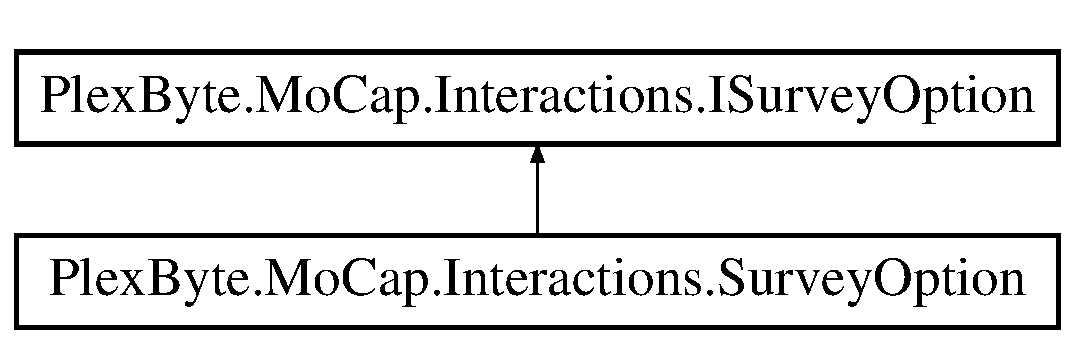
\includegraphics[height=2.000000cm]{interface_plex_byte_1_1_mo_cap_1_1_interactions_1_1_i_survey_option}
\end{center}
\end{figure}
\subsection*{Properties}
\begin{DoxyCompactItemize}
\item 
string \hyperlink{interface_plex_byte_1_1_mo_cap_1_1_interactions_1_1_i_survey_option_a49da68b97f711aa9708ad94b512a8be9}{Text}\hspace{0.3cm}{\ttfamily  \mbox{[}get\mbox{]}}
\item 
Date\+Time \hyperlink{interface_plex_byte_1_1_mo_cap_1_1_interactions_1_1_i_survey_option_a7fce51617a89b3d3b4ebd804b8b9c6af}{Created\+Date\+Time}\hspace{0.3cm}{\ttfamily  \mbox{[}get\mbox{]}}
\item 
string \hyperlink{interface_plex_byte_1_1_mo_cap_1_1_interactions_1_1_i_survey_option_a837c0227b5d8bf74254e1f218eb37148}{Id}\hspace{0.3cm}{\ttfamily  \mbox{[}get\mbox{]}}
\end{DoxyCompactItemize}


\subsection{Detailed Description}
The survey option interface 



Definition at line 12 of file I\+Survey\+Option.\+cs.



\subsection{Property Documentation}
\index{Plex\+Byte\+::\+Mo\+Cap\+::\+Interactions\+::\+I\+Survey\+Option@{Plex\+Byte\+::\+Mo\+Cap\+::\+Interactions\+::\+I\+Survey\+Option}!Created\+Date\+Time@{Created\+Date\+Time}}
\index{Created\+Date\+Time@{Created\+Date\+Time}!Plex\+Byte\+::\+Mo\+Cap\+::\+Interactions\+::\+I\+Survey\+Option@{Plex\+Byte\+::\+Mo\+Cap\+::\+Interactions\+::\+I\+Survey\+Option}}
\subsubsection[{\texorpdfstring{Created\+Date\+Time}{CreatedDateTime}}]{\setlength{\rightskip}{0pt plus 5cm}Date\+Time Plex\+Byte.\+Mo\+Cap.\+Interactions.\+I\+Survey\+Option.\+Created\+Date\+Time\hspace{0.3cm}{\ttfamily [get]}}\hypertarget{interface_plex_byte_1_1_mo_cap_1_1_interactions_1_1_i_survey_option_a7fce51617a89b3d3b4ebd804b8b9c6af}{}\label{interface_plex_byte_1_1_mo_cap_1_1_interactions_1_1_i_survey_option_a7fce51617a89b3d3b4ebd804b8b9c6af}


Definition at line 16 of file I\+Survey\+Option.\+cs.

\index{Plex\+Byte\+::\+Mo\+Cap\+::\+Interactions\+::\+I\+Survey\+Option@{Plex\+Byte\+::\+Mo\+Cap\+::\+Interactions\+::\+I\+Survey\+Option}!Id@{Id}}
\index{Id@{Id}!Plex\+Byte\+::\+Mo\+Cap\+::\+Interactions\+::\+I\+Survey\+Option@{Plex\+Byte\+::\+Mo\+Cap\+::\+Interactions\+::\+I\+Survey\+Option}}
\subsubsection[{\texorpdfstring{Id}{Id}}]{\setlength{\rightskip}{0pt plus 5cm}string Plex\+Byte.\+Mo\+Cap.\+Interactions.\+I\+Survey\+Option.\+Id\hspace{0.3cm}{\ttfamily [get]}}\hypertarget{interface_plex_byte_1_1_mo_cap_1_1_interactions_1_1_i_survey_option_a837c0227b5d8bf74254e1f218eb37148}{}\label{interface_plex_byte_1_1_mo_cap_1_1_interactions_1_1_i_survey_option_a837c0227b5d8bf74254e1f218eb37148}


Definition at line 18 of file I\+Survey\+Option.\+cs.

\index{Plex\+Byte\+::\+Mo\+Cap\+::\+Interactions\+::\+I\+Survey\+Option@{Plex\+Byte\+::\+Mo\+Cap\+::\+Interactions\+::\+I\+Survey\+Option}!Text@{Text}}
\index{Text@{Text}!Plex\+Byte\+::\+Mo\+Cap\+::\+Interactions\+::\+I\+Survey\+Option@{Plex\+Byte\+::\+Mo\+Cap\+::\+Interactions\+::\+I\+Survey\+Option}}
\subsubsection[{\texorpdfstring{Text}{Text}}]{\setlength{\rightskip}{0pt plus 5cm}string Plex\+Byte.\+Mo\+Cap.\+Interactions.\+I\+Survey\+Option.\+Text\hspace{0.3cm}{\ttfamily [get]}}\hypertarget{interface_plex_byte_1_1_mo_cap_1_1_interactions_1_1_i_survey_option_a49da68b97f711aa9708ad94b512a8be9}{}\label{interface_plex_byte_1_1_mo_cap_1_1_interactions_1_1_i_survey_option_a49da68b97f711aa9708ad94b512a8be9}


Definition at line 14 of file I\+Survey\+Option.\+cs.



The documentation for this interface was generated from the following file\+:\begin{DoxyCompactItemize}
\item 
D\+:/\+Users/\+Christian\+B/\+Documents/\+\_\+\+H\+F Infomatik/\+Git\+Hub\+\_\+\+Repos/\+Mo\+Cap/\+Plex\+Byte.\+Mo\+Cap/\+Plex\+Byte.\+Mo\+Cap.\+Interactions/\hyperlink{_i_survey_option_8cs}{I\+Survey\+Option.\+cs}\end{DoxyCompactItemize}

\hypertarget{interface_plex_byte_1_1_mo_cap_1_1_interactions_1_1_i_task}{}\section{Plex\+Byte.\+Mo\+Cap.\+Interactions.\+I\+Task Interface Reference}
\label{interface_plex_byte_1_1_mo_cap_1_1_interactions_1_1_i_task}\index{Plex\+Byte.\+Mo\+Cap.\+Interactions.\+I\+Task@{Plex\+Byte.\+Mo\+Cap.\+Interactions.\+I\+Task}}
Inheritance diagram for Plex\+Byte.\+Mo\+Cap.\+Interactions.\+I\+Task\+:\begin{figure}[H]
\begin{center}
\leavevmode
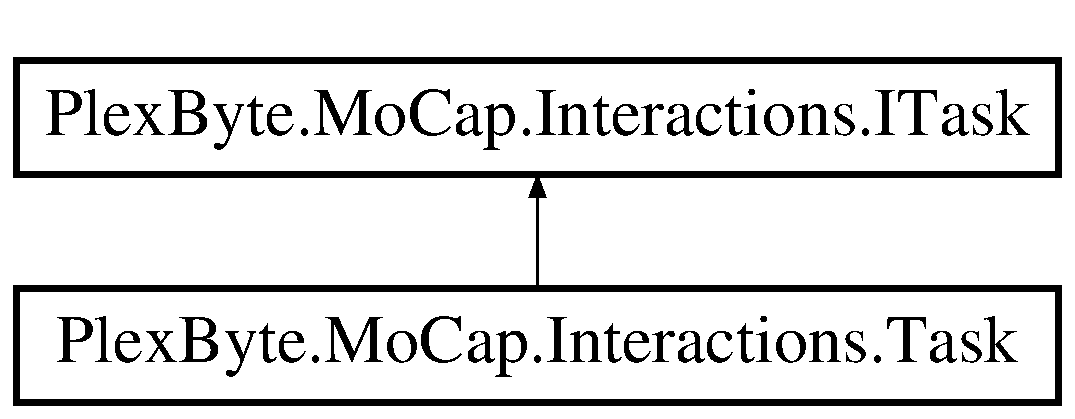
\includegraphics[height=2.000000cm]{interface_plex_byte_1_1_mo_cap_1_1_interactions_1_1_i_task}
\end{center}
\end{figure}
\subsection*{Public Member Functions}
\begin{DoxyCompactItemize}
\item 
void \hyperlink{interface_plex_byte_1_1_mo_cap_1_1_interactions_1_1_i_task_af70a3a36f24fedda95ad55714333090f}{Add\+Timeslice} (int p\+Duration)
\item 
void \hyperlink{interface_plex_byte_1_1_mo_cap_1_1_interactions_1_1_i_task_a96b54ce198b08eccb95456e16c4538d5}{Add\+Expense} (decimal p\+Expense\+Value)
\item 
void \hyperlink{interface_plex_byte_1_1_mo_cap_1_1_interactions_1_1_i_task_a7e385a390973b7cc165bfbb6caf9ed75}{Udate\+Progress} (int p\+Progress)
\item 
void \hyperlink{interface_plex_byte_1_1_mo_cap_1_1_interactions_1_1_i_task_a20a23d8d8abb9f14330e75e8e09fe263}{Add\+Sub\+Task} (\hyperlink{interface_plex_byte_1_1_mo_cap_1_1_interactions_1_1_i_task}{I\+Task} p\+Task)
\end{DoxyCompactItemize}
\subsection*{Properties}
\begin{DoxyCompactItemize}
\item 
string \hyperlink{interface_plex_byte_1_1_mo_cap_1_1_interactions_1_1_i_task_a7e207370f422edc06071f3c288ac56a2}{Id}\hspace{0.3cm}{\ttfamily  \mbox{[}get\mbox{]}}
\item 
string \hyperlink{interface_plex_byte_1_1_mo_cap_1_1_interactions_1_1_i_task_afb97aa4ca4a2b2c1f1dc7bc38b08264e}{Interaction\+Id}\hspace{0.3cm}{\ttfamily  \mbox{[}get, set\mbox{]}}
\item 
string \hyperlink{interface_plex_byte_1_1_mo_cap_1_1_interactions_1_1_i_task_a5b3f6564ac365dfb2fe404e91a688286}{Project\+Id}\hspace{0.3cm}{\ttfamily  \mbox{[}get, set\mbox{]}}
\item 
Date\+Time \hyperlink{interface_plex_byte_1_1_mo_cap_1_1_interactions_1_1_i_task_a514288c26d32ef108bfddc81ef45bb1f}{Due\+Date\+Time}\hspace{0.3cm}{\ttfamily  \mbox{[}get\mbox{]}}
\item 
decimal \hyperlink{interface_plex_byte_1_1_mo_cap_1_1_interactions_1_1_i_task_a663dcda655843c2a6671d9d119b213e9}{Budget}\hspace{0.3cm}{\ttfamily  \mbox{[}get\mbox{]}}
\item 
int \hyperlink{interface_plex_byte_1_1_mo_cap_1_1_interactions_1_1_i_task_a8f8d9d6893e519866c5e7f0577bc9599}{Duration}\hspace{0.3cm}{\ttfamily  \mbox{[}get\mbox{]}}
\item 
int \hyperlink{interface_plex_byte_1_1_mo_cap_1_1_interactions_1_1_i_task_a98be225725e6e45fac01e73367da498e}{Priority}\hspace{0.3cm}{\ttfamily  \mbox{[}get\mbox{]}}
\item 
int \hyperlink{interface_plex_byte_1_1_mo_cap_1_1_interactions_1_1_i_task_a70cd0b5fcf58544ba8f8281cb8f21e97}{Progress}\hspace{0.3cm}{\ttfamily  \mbox{[}get\mbox{]}}
\item 
int \hyperlink{interface_plex_byte_1_1_mo_cap_1_1_interactions_1_1_i_task_a8a3ed76e09b91a0332ce84629bdac670}{Duration\+Current}\hspace{0.3cm}{\ttfamily  \mbox{[}get\mbox{]}}
\item 
decimal \hyperlink{interface_plex_byte_1_1_mo_cap_1_1_interactions_1_1_i_task_a39128d958f8f9c4dcba4a6c3e48d782d}{Budget\+Used}\hspace{0.3cm}{\ttfamily  \mbox{[}get\mbox{]}}
\item 
string \hyperlink{interface_plex_byte_1_1_mo_cap_1_1_interactions_1_1_i_task_a253ea25ebaf91c0307d4cbff0a8d4144}{Title}\hspace{0.3cm}{\ttfamily  \mbox{[}get, set\mbox{]}}
\item 
List$<$ \hyperlink{interface_plex_byte_1_1_mo_cap_1_1_interactions_1_1_i_task}{I\+Task} $>$ \hyperlink{interface_plex_byte_1_1_mo_cap_1_1_interactions_1_1_i_task_ac8f4d55c1b23a55959e86b9fb8f15d0e}{Sub\+Tasks}\hspace{0.3cm}{\ttfamily  \mbox{[}get\mbox{]}}
\end{DoxyCompactItemize}


\subsection{Detailed Description}


Definition at line 12 of file I\+Task.\+cs.



\subsection{Member Function Documentation}
\index{Plex\+Byte\+::\+Mo\+Cap\+::\+Interactions\+::\+I\+Task@{Plex\+Byte\+::\+Mo\+Cap\+::\+Interactions\+::\+I\+Task}!Add\+Expense@{Add\+Expense}}
\index{Add\+Expense@{Add\+Expense}!Plex\+Byte\+::\+Mo\+Cap\+::\+Interactions\+::\+I\+Task@{Plex\+Byte\+::\+Mo\+Cap\+::\+Interactions\+::\+I\+Task}}
\subsubsection[{\texorpdfstring{Add\+Expense(decimal p\+Expense\+Value)}{AddExpense(decimal pExpenseValue)}}]{\setlength{\rightskip}{0pt plus 5cm}void Plex\+Byte.\+Mo\+Cap.\+Interactions.\+I\+Task.\+Add\+Expense (
\begin{DoxyParamCaption}
\item[{decimal}]{p\+Expense\+Value}
\end{DoxyParamCaption}
)}\hypertarget{interface_plex_byte_1_1_mo_cap_1_1_interactions_1_1_i_task_a96b54ce198b08eccb95456e16c4538d5}{}\label{interface_plex_byte_1_1_mo_cap_1_1_interactions_1_1_i_task_a96b54ce198b08eccb95456e16c4538d5}


Implemented in \hyperlink{class_plex_byte_1_1_mo_cap_1_1_interactions_1_1_task_a12136bc5d5722e10c4a20b4e9ab40788}{Plex\+Byte.\+Mo\+Cap.\+Interactions.\+Task}.

\index{Plex\+Byte\+::\+Mo\+Cap\+::\+Interactions\+::\+I\+Task@{Plex\+Byte\+::\+Mo\+Cap\+::\+Interactions\+::\+I\+Task}!Add\+Sub\+Task@{Add\+Sub\+Task}}
\index{Add\+Sub\+Task@{Add\+Sub\+Task}!Plex\+Byte\+::\+Mo\+Cap\+::\+Interactions\+::\+I\+Task@{Plex\+Byte\+::\+Mo\+Cap\+::\+Interactions\+::\+I\+Task}}
\subsubsection[{\texorpdfstring{Add\+Sub\+Task(\+I\+Task p\+Task)}{AddSubTask(ITask pTask)}}]{\setlength{\rightskip}{0pt plus 5cm}void Plex\+Byte.\+Mo\+Cap.\+Interactions.\+I\+Task.\+Add\+Sub\+Task (
\begin{DoxyParamCaption}
\item[{{\bf I\+Task}}]{p\+Task}
\end{DoxyParamCaption}
)}\hypertarget{interface_plex_byte_1_1_mo_cap_1_1_interactions_1_1_i_task_a20a23d8d8abb9f14330e75e8e09fe263}{}\label{interface_plex_byte_1_1_mo_cap_1_1_interactions_1_1_i_task_a20a23d8d8abb9f14330e75e8e09fe263}


Implemented in \hyperlink{class_plex_byte_1_1_mo_cap_1_1_interactions_1_1_task_aa152325c4d018f68b8dcbe1ef4c46497}{Plex\+Byte.\+Mo\+Cap.\+Interactions.\+Task}.

\index{Plex\+Byte\+::\+Mo\+Cap\+::\+Interactions\+::\+I\+Task@{Plex\+Byte\+::\+Mo\+Cap\+::\+Interactions\+::\+I\+Task}!Add\+Timeslice@{Add\+Timeslice}}
\index{Add\+Timeslice@{Add\+Timeslice}!Plex\+Byte\+::\+Mo\+Cap\+::\+Interactions\+::\+I\+Task@{Plex\+Byte\+::\+Mo\+Cap\+::\+Interactions\+::\+I\+Task}}
\subsubsection[{\texorpdfstring{Add\+Timeslice(int p\+Duration)}{AddTimeslice(int pDuration)}}]{\setlength{\rightskip}{0pt plus 5cm}void Plex\+Byte.\+Mo\+Cap.\+Interactions.\+I\+Task.\+Add\+Timeslice (
\begin{DoxyParamCaption}
\item[{int}]{p\+Duration}
\end{DoxyParamCaption}
)}\hypertarget{interface_plex_byte_1_1_mo_cap_1_1_interactions_1_1_i_task_af70a3a36f24fedda95ad55714333090f}{}\label{interface_plex_byte_1_1_mo_cap_1_1_interactions_1_1_i_task_af70a3a36f24fedda95ad55714333090f}


Implemented in \hyperlink{class_plex_byte_1_1_mo_cap_1_1_interactions_1_1_task_ab8d71506e5343bc302bb661a5131449b}{Plex\+Byte.\+Mo\+Cap.\+Interactions.\+Task}.

\index{Plex\+Byte\+::\+Mo\+Cap\+::\+Interactions\+::\+I\+Task@{Plex\+Byte\+::\+Mo\+Cap\+::\+Interactions\+::\+I\+Task}!Udate\+Progress@{Udate\+Progress}}
\index{Udate\+Progress@{Udate\+Progress}!Plex\+Byte\+::\+Mo\+Cap\+::\+Interactions\+::\+I\+Task@{Plex\+Byte\+::\+Mo\+Cap\+::\+Interactions\+::\+I\+Task}}
\subsubsection[{\texorpdfstring{Udate\+Progress(int p\+Progress)}{UdateProgress(int pProgress)}}]{\setlength{\rightskip}{0pt plus 5cm}void Plex\+Byte.\+Mo\+Cap.\+Interactions.\+I\+Task.\+Udate\+Progress (
\begin{DoxyParamCaption}
\item[{int}]{p\+Progress}
\end{DoxyParamCaption}
)}\hypertarget{interface_plex_byte_1_1_mo_cap_1_1_interactions_1_1_i_task_a7e385a390973b7cc165bfbb6caf9ed75}{}\label{interface_plex_byte_1_1_mo_cap_1_1_interactions_1_1_i_task_a7e385a390973b7cc165bfbb6caf9ed75}


Implemented in \hyperlink{class_plex_byte_1_1_mo_cap_1_1_interactions_1_1_task_af28b4349816bcd4d60c0746e7b7425d4}{Plex\+Byte.\+Mo\+Cap.\+Interactions.\+Task}.



\subsection{Property Documentation}
\index{Plex\+Byte\+::\+Mo\+Cap\+::\+Interactions\+::\+I\+Task@{Plex\+Byte\+::\+Mo\+Cap\+::\+Interactions\+::\+I\+Task}!Budget@{Budget}}
\index{Budget@{Budget}!Plex\+Byte\+::\+Mo\+Cap\+::\+Interactions\+::\+I\+Task@{Plex\+Byte\+::\+Mo\+Cap\+::\+Interactions\+::\+I\+Task}}
\subsubsection[{\texorpdfstring{Budget}{Budget}}]{\setlength{\rightskip}{0pt plus 5cm}decimal Plex\+Byte.\+Mo\+Cap.\+Interactions.\+I\+Task.\+Budget\hspace{0.3cm}{\ttfamily [get]}}\hypertarget{interface_plex_byte_1_1_mo_cap_1_1_interactions_1_1_i_task_a663dcda655843c2a6671d9d119b213e9}{}\label{interface_plex_byte_1_1_mo_cap_1_1_interactions_1_1_i_task_a663dcda655843c2a6671d9d119b213e9}


Definition at line 22 of file I\+Task.\+cs.

\index{Plex\+Byte\+::\+Mo\+Cap\+::\+Interactions\+::\+I\+Task@{Plex\+Byte\+::\+Mo\+Cap\+::\+Interactions\+::\+I\+Task}!Budget\+Used@{Budget\+Used}}
\index{Budget\+Used@{Budget\+Used}!Plex\+Byte\+::\+Mo\+Cap\+::\+Interactions\+::\+I\+Task@{Plex\+Byte\+::\+Mo\+Cap\+::\+Interactions\+::\+I\+Task}}
\subsubsection[{\texorpdfstring{Budget\+Used}{BudgetUsed}}]{\setlength{\rightskip}{0pt plus 5cm}decimal Plex\+Byte.\+Mo\+Cap.\+Interactions.\+I\+Task.\+Budget\+Used\hspace{0.3cm}{\ttfamily [get]}}\hypertarget{interface_plex_byte_1_1_mo_cap_1_1_interactions_1_1_i_task_a39128d958f8f9c4dcba4a6c3e48d782d}{}\label{interface_plex_byte_1_1_mo_cap_1_1_interactions_1_1_i_task_a39128d958f8f9c4dcba4a6c3e48d782d}


Definition at line 32 of file I\+Task.\+cs.

\index{Plex\+Byte\+::\+Mo\+Cap\+::\+Interactions\+::\+I\+Task@{Plex\+Byte\+::\+Mo\+Cap\+::\+Interactions\+::\+I\+Task}!Due\+Date\+Time@{Due\+Date\+Time}}
\index{Due\+Date\+Time@{Due\+Date\+Time}!Plex\+Byte\+::\+Mo\+Cap\+::\+Interactions\+::\+I\+Task@{Plex\+Byte\+::\+Mo\+Cap\+::\+Interactions\+::\+I\+Task}}
\subsubsection[{\texorpdfstring{Due\+Date\+Time}{DueDateTime}}]{\setlength{\rightskip}{0pt plus 5cm}Date\+Time Plex\+Byte.\+Mo\+Cap.\+Interactions.\+I\+Task.\+Due\+Date\+Time\hspace{0.3cm}{\ttfamily [get]}}\hypertarget{interface_plex_byte_1_1_mo_cap_1_1_interactions_1_1_i_task_a514288c26d32ef108bfddc81ef45bb1f}{}\label{interface_plex_byte_1_1_mo_cap_1_1_interactions_1_1_i_task_a514288c26d32ef108bfddc81ef45bb1f}


Definition at line 20 of file I\+Task.\+cs.

\index{Plex\+Byte\+::\+Mo\+Cap\+::\+Interactions\+::\+I\+Task@{Plex\+Byte\+::\+Mo\+Cap\+::\+Interactions\+::\+I\+Task}!Duration@{Duration}}
\index{Duration@{Duration}!Plex\+Byte\+::\+Mo\+Cap\+::\+Interactions\+::\+I\+Task@{Plex\+Byte\+::\+Mo\+Cap\+::\+Interactions\+::\+I\+Task}}
\subsubsection[{\texorpdfstring{Duration}{Duration}}]{\setlength{\rightskip}{0pt plus 5cm}int Plex\+Byte.\+Mo\+Cap.\+Interactions.\+I\+Task.\+Duration\hspace{0.3cm}{\ttfamily [get]}}\hypertarget{interface_plex_byte_1_1_mo_cap_1_1_interactions_1_1_i_task_a8f8d9d6893e519866c5e7f0577bc9599}{}\label{interface_plex_byte_1_1_mo_cap_1_1_interactions_1_1_i_task_a8f8d9d6893e519866c5e7f0577bc9599}


Definition at line 24 of file I\+Task.\+cs.

\index{Plex\+Byte\+::\+Mo\+Cap\+::\+Interactions\+::\+I\+Task@{Plex\+Byte\+::\+Mo\+Cap\+::\+Interactions\+::\+I\+Task}!Duration\+Current@{Duration\+Current}}
\index{Duration\+Current@{Duration\+Current}!Plex\+Byte\+::\+Mo\+Cap\+::\+Interactions\+::\+I\+Task@{Plex\+Byte\+::\+Mo\+Cap\+::\+Interactions\+::\+I\+Task}}
\subsubsection[{\texorpdfstring{Duration\+Current}{DurationCurrent}}]{\setlength{\rightskip}{0pt plus 5cm}int Plex\+Byte.\+Mo\+Cap.\+Interactions.\+I\+Task.\+Duration\+Current\hspace{0.3cm}{\ttfamily [get]}}\hypertarget{interface_plex_byte_1_1_mo_cap_1_1_interactions_1_1_i_task_a8a3ed76e09b91a0332ce84629bdac670}{}\label{interface_plex_byte_1_1_mo_cap_1_1_interactions_1_1_i_task_a8a3ed76e09b91a0332ce84629bdac670}


Definition at line 30 of file I\+Task.\+cs.

\index{Plex\+Byte\+::\+Mo\+Cap\+::\+Interactions\+::\+I\+Task@{Plex\+Byte\+::\+Mo\+Cap\+::\+Interactions\+::\+I\+Task}!Id@{Id}}
\index{Id@{Id}!Plex\+Byte\+::\+Mo\+Cap\+::\+Interactions\+::\+I\+Task@{Plex\+Byte\+::\+Mo\+Cap\+::\+Interactions\+::\+I\+Task}}
\subsubsection[{\texorpdfstring{Id}{Id}}]{\setlength{\rightskip}{0pt plus 5cm}string Plex\+Byte.\+Mo\+Cap.\+Interactions.\+I\+Task.\+Id\hspace{0.3cm}{\ttfamily [get]}}\hypertarget{interface_plex_byte_1_1_mo_cap_1_1_interactions_1_1_i_task_a7e207370f422edc06071f3c288ac56a2}{}\label{interface_plex_byte_1_1_mo_cap_1_1_interactions_1_1_i_task_a7e207370f422edc06071f3c288ac56a2}


Definition at line 14 of file I\+Task.\+cs.

\index{Plex\+Byte\+::\+Mo\+Cap\+::\+Interactions\+::\+I\+Task@{Plex\+Byte\+::\+Mo\+Cap\+::\+Interactions\+::\+I\+Task}!Interaction\+Id@{Interaction\+Id}}
\index{Interaction\+Id@{Interaction\+Id}!Plex\+Byte\+::\+Mo\+Cap\+::\+Interactions\+::\+I\+Task@{Plex\+Byte\+::\+Mo\+Cap\+::\+Interactions\+::\+I\+Task}}
\subsubsection[{\texorpdfstring{Interaction\+Id}{InteractionId}}]{\setlength{\rightskip}{0pt plus 5cm}string Plex\+Byte.\+Mo\+Cap.\+Interactions.\+I\+Task.\+Interaction\+Id\hspace{0.3cm}{\ttfamily [get]}, {\ttfamily [set]}}\hypertarget{interface_plex_byte_1_1_mo_cap_1_1_interactions_1_1_i_task_afb97aa4ca4a2b2c1f1dc7bc38b08264e}{}\label{interface_plex_byte_1_1_mo_cap_1_1_interactions_1_1_i_task_afb97aa4ca4a2b2c1f1dc7bc38b08264e}


Definition at line 16 of file I\+Task.\+cs.

\index{Plex\+Byte\+::\+Mo\+Cap\+::\+Interactions\+::\+I\+Task@{Plex\+Byte\+::\+Mo\+Cap\+::\+Interactions\+::\+I\+Task}!Priority@{Priority}}
\index{Priority@{Priority}!Plex\+Byte\+::\+Mo\+Cap\+::\+Interactions\+::\+I\+Task@{Plex\+Byte\+::\+Mo\+Cap\+::\+Interactions\+::\+I\+Task}}
\subsubsection[{\texorpdfstring{Priority}{Priority}}]{\setlength{\rightskip}{0pt plus 5cm}int Plex\+Byte.\+Mo\+Cap.\+Interactions.\+I\+Task.\+Priority\hspace{0.3cm}{\ttfamily [get]}}\hypertarget{interface_plex_byte_1_1_mo_cap_1_1_interactions_1_1_i_task_a98be225725e6e45fac01e73367da498e}{}\label{interface_plex_byte_1_1_mo_cap_1_1_interactions_1_1_i_task_a98be225725e6e45fac01e73367da498e}


Definition at line 26 of file I\+Task.\+cs.

\index{Plex\+Byte\+::\+Mo\+Cap\+::\+Interactions\+::\+I\+Task@{Plex\+Byte\+::\+Mo\+Cap\+::\+Interactions\+::\+I\+Task}!Progress@{Progress}}
\index{Progress@{Progress}!Plex\+Byte\+::\+Mo\+Cap\+::\+Interactions\+::\+I\+Task@{Plex\+Byte\+::\+Mo\+Cap\+::\+Interactions\+::\+I\+Task}}
\subsubsection[{\texorpdfstring{Progress}{Progress}}]{\setlength{\rightskip}{0pt plus 5cm}int Plex\+Byte.\+Mo\+Cap.\+Interactions.\+I\+Task.\+Progress\hspace{0.3cm}{\ttfamily [get]}}\hypertarget{interface_plex_byte_1_1_mo_cap_1_1_interactions_1_1_i_task_a70cd0b5fcf58544ba8f8281cb8f21e97}{}\label{interface_plex_byte_1_1_mo_cap_1_1_interactions_1_1_i_task_a70cd0b5fcf58544ba8f8281cb8f21e97}


Definition at line 28 of file I\+Task.\+cs.

\index{Plex\+Byte\+::\+Mo\+Cap\+::\+Interactions\+::\+I\+Task@{Plex\+Byte\+::\+Mo\+Cap\+::\+Interactions\+::\+I\+Task}!Project\+Id@{Project\+Id}}
\index{Project\+Id@{Project\+Id}!Plex\+Byte\+::\+Mo\+Cap\+::\+Interactions\+::\+I\+Task@{Plex\+Byte\+::\+Mo\+Cap\+::\+Interactions\+::\+I\+Task}}
\subsubsection[{\texorpdfstring{Project\+Id}{ProjectId}}]{\setlength{\rightskip}{0pt plus 5cm}string Plex\+Byte.\+Mo\+Cap.\+Interactions.\+I\+Task.\+Project\+Id\hspace{0.3cm}{\ttfamily [get]}, {\ttfamily [set]}}\hypertarget{interface_plex_byte_1_1_mo_cap_1_1_interactions_1_1_i_task_a5b3f6564ac365dfb2fe404e91a688286}{}\label{interface_plex_byte_1_1_mo_cap_1_1_interactions_1_1_i_task_a5b3f6564ac365dfb2fe404e91a688286}


Definition at line 18 of file I\+Task.\+cs.

\index{Plex\+Byte\+::\+Mo\+Cap\+::\+Interactions\+::\+I\+Task@{Plex\+Byte\+::\+Mo\+Cap\+::\+Interactions\+::\+I\+Task}!Sub\+Tasks@{Sub\+Tasks}}
\index{Sub\+Tasks@{Sub\+Tasks}!Plex\+Byte\+::\+Mo\+Cap\+::\+Interactions\+::\+I\+Task@{Plex\+Byte\+::\+Mo\+Cap\+::\+Interactions\+::\+I\+Task}}
\subsubsection[{\texorpdfstring{Sub\+Tasks}{SubTasks}}]{\setlength{\rightskip}{0pt plus 5cm}List$<${\bf I\+Task}$>$ Plex\+Byte.\+Mo\+Cap.\+Interactions.\+I\+Task.\+Sub\+Tasks\hspace{0.3cm}{\ttfamily [get]}}\hypertarget{interface_plex_byte_1_1_mo_cap_1_1_interactions_1_1_i_task_ac8f4d55c1b23a55959e86b9fb8f15d0e}{}\label{interface_plex_byte_1_1_mo_cap_1_1_interactions_1_1_i_task_ac8f4d55c1b23a55959e86b9fb8f15d0e}


Definition at line 36 of file I\+Task.\+cs.

\index{Plex\+Byte\+::\+Mo\+Cap\+::\+Interactions\+::\+I\+Task@{Plex\+Byte\+::\+Mo\+Cap\+::\+Interactions\+::\+I\+Task}!Title@{Title}}
\index{Title@{Title}!Plex\+Byte\+::\+Mo\+Cap\+::\+Interactions\+::\+I\+Task@{Plex\+Byte\+::\+Mo\+Cap\+::\+Interactions\+::\+I\+Task}}
\subsubsection[{\texorpdfstring{Title}{Title}}]{\setlength{\rightskip}{0pt plus 5cm}string Plex\+Byte.\+Mo\+Cap.\+Interactions.\+I\+Task.\+Title\hspace{0.3cm}{\ttfamily [get]}, {\ttfamily [set]}}\hypertarget{interface_plex_byte_1_1_mo_cap_1_1_interactions_1_1_i_task_a253ea25ebaf91c0307d4cbff0a8d4144}{}\label{interface_plex_byte_1_1_mo_cap_1_1_interactions_1_1_i_task_a253ea25ebaf91c0307d4cbff0a8d4144}


Definition at line 34 of file I\+Task.\+cs.



The documentation for this interface was generated from the following file\+:\begin{DoxyCompactItemize}
\item 
D\+:/\+Users/\+Christian\+B/\+Documents/\+\_\+\+H\+F Infomatik/\+Git\+Hub\+\_\+\+Repos/\+Mo\+Cap/\+Plex\+Byte.\+Mo\+Cap/\+Plex\+Byte.\+Mo\+Cap.\+Interactions/\hyperlink{_i_task_8cs}{I\+Task.\+cs}\end{DoxyCompactItemize}

\hypertarget{interface_plex_byte_1_1_mo_cap_1_1_interactions_1_1_i_timeslice}{}\section{Plex\+Byte.\+Mo\+Cap.\+Interactions.\+I\+Timeslice Interface Reference}
\label{interface_plex_byte_1_1_mo_cap_1_1_interactions_1_1_i_timeslice}\index{Plex\+Byte.\+Mo\+Cap.\+Interactions.\+I\+Timeslice@{Plex\+Byte.\+Mo\+Cap.\+Interactions.\+I\+Timeslice}}
Inheritance diagram for Plex\+Byte.\+Mo\+Cap.\+Interactions.\+I\+Timeslice\+:\begin{figure}[H]
\begin{center}
\leavevmode
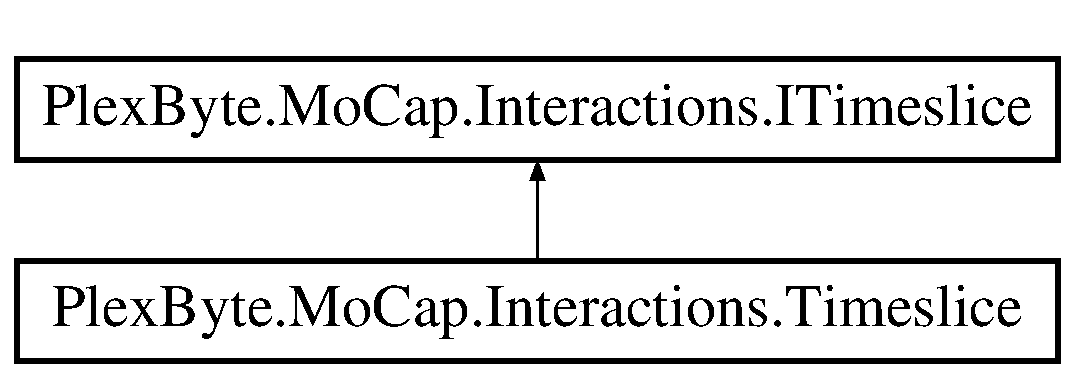
\includegraphics[height=2.000000cm]{interface_plex_byte_1_1_mo_cap_1_1_interactions_1_1_i_timeslice}
\end{center}
\end{figure}
\subsection*{Public Member Functions}
\begin{DoxyCompactItemize}
\item 
int \hyperlink{interface_plex_byte_1_1_mo_cap_1_1_interactions_1_1_i_timeslice_a4cf2fbe8712024476536bd187dab494c}{Calculate\+Duration} (Date\+Time p\+Start\+DT, Date\+Time p\+End\+DT)
\end{DoxyCompactItemize}
\subsection*{Properties}
\begin{DoxyCompactItemize}
\item 
int \hyperlink{interface_plex_byte_1_1_mo_cap_1_1_interactions_1_1_i_timeslice_ae5913fb8d9d7a5b4de9b9b9a4acd94be}{Duration}\hspace{0.3cm}{\ttfamily  \mbox{[}get\mbox{]}}
\item 
string \hyperlink{interface_plex_byte_1_1_mo_cap_1_1_interactions_1_1_i_timeslice_ad37b8578c03d8e90956a670b9a70bcbd}{Description}\hspace{0.3cm}{\ttfamily  \mbox{[}get, set\mbox{]}}
\item 
I\+User \hyperlink{interface_plex_byte_1_1_mo_cap_1_1_interactions_1_1_i_timeslice_a719ec23a47825e45f4106f1c50a08804}{User}\hspace{0.3cm}{\ttfamily  \mbox{[}get\mbox{]}}
\item 
\hyperlink{interface_plex_byte_1_1_mo_cap_1_1_interactions_1_1_i_interaction}{I\+Interaction} \hyperlink{interface_plex_byte_1_1_mo_cap_1_1_interactions_1_1_i_timeslice_a1b70f9e866de9e39c2de1bc4db02d629}{Target}\hspace{0.3cm}{\ttfamily  \mbox{[}get\mbox{]}}
\item 
Date\+Time \hyperlink{interface_plex_byte_1_1_mo_cap_1_1_interactions_1_1_i_timeslice_ae32d625997888202222bc31e4d8e1f17}{Created\+Date\+Time}\hspace{0.3cm}{\ttfamily  \mbox{[}get, set\mbox{]}}
\item 
Date\+Time \hyperlink{interface_plex_byte_1_1_mo_cap_1_1_interactions_1_1_i_timeslice_adebf67921d263827545fa2f8f97d3b50}{Modified\+Date\+Time}\hspace{0.3cm}{\ttfamily  \mbox{[}get, set\mbox{]}}
\end{DoxyCompactItemize}


\subsection{Detailed Description}


Definition at line 10 of file I\+Timeslice.\+cs.



\subsection{Member Function Documentation}
\index{Plex\+Byte\+::\+Mo\+Cap\+::\+Interactions\+::\+I\+Timeslice@{Plex\+Byte\+::\+Mo\+Cap\+::\+Interactions\+::\+I\+Timeslice}!Calculate\+Duration@{Calculate\+Duration}}
\index{Calculate\+Duration@{Calculate\+Duration}!Plex\+Byte\+::\+Mo\+Cap\+::\+Interactions\+::\+I\+Timeslice@{Plex\+Byte\+::\+Mo\+Cap\+::\+Interactions\+::\+I\+Timeslice}}
\subsubsection[{\texorpdfstring{Calculate\+Duration(\+Date\+Time p\+Start\+D\+T, Date\+Time p\+End\+D\+T)}{CalculateDuration(DateTime pStartDT, DateTime pEndDT)}}]{\setlength{\rightskip}{0pt plus 5cm}int Plex\+Byte.\+Mo\+Cap.\+Interactions.\+I\+Timeslice.\+Calculate\+Duration (
\begin{DoxyParamCaption}
\item[{Date\+Time}]{p\+Start\+DT, }
\item[{Date\+Time}]{p\+End\+DT}
\end{DoxyParamCaption}
)}\hypertarget{interface_plex_byte_1_1_mo_cap_1_1_interactions_1_1_i_timeslice_a4cf2fbe8712024476536bd187dab494c}{}\label{interface_plex_byte_1_1_mo_cap_1_1_interactions_1_1_i_timeslice_a4cf2fbe8712024476536bd187dab494c}


Implemented in \hyperlink{class_plex_byte_1_1_mo_cap_1_1_interactions_1_1_timeslice_acf019f3b3bfe9c64fc32d78e45c41f8a}{Plex\+Byte.\+Mo\+Cap.\+Interactions.\+Timeslice}.



\subsection{Property Documentation}
\index{Plex\+Byte\+::\+Mo\+Cap\+::\+Interactions\+::\+I\+Timeslice@{Plex\+Byte\+::\+Mo\+Cap\+::\+Interactions\+::\+I\+Timeslice}!Created\+Date\+Time@{Created\+Date\+Time}}
\index{Created\+Date\+Time@{Created\+Date\+Time}!Plex\+Byte\+::\+Mo\+Cap\+::\+Interactions\+::\+I\+Timeslice@{Plex\+Byte\+::\+Mo\+Cap\+::\+Interactions\+::\+I\+Timeslice}}
\subsubsection[{\texorpdfstring{Created\+Date\+Time}{CreatedDateTime}}]{\setlength{\rightskip}{0pt plus 5cm}Date\+Time Plex\+Byte.\+Mo\+Cap.\+Interactions.\+I\+Timeslice.\+Created\+Date\+Time\hspace{0.3cm}{\ttfamily [get]}, {\ttfamily [set]}}\hypertarget{interface_plex_byte_1_1_mo_cap_1_1_interactions_1_1_i_timeslice_ae32d625997888202222bc31e4d8e1f17}{}\label{interface_plex_byte_1_1_mo_cap_1_1_interactions_1_1_i_timeslice_ae32d625997888202222bc31e4d8e1f17}


Definition at line 20 of file I\+Timeslice.\+cs.

\index{Plex\+Byte\+::\+Mo\+Cap\+::\+Interactions\+::\+I\+Timeslice@{Plex\+Byte\+::\+Mo\+Cap\+::\+Interactions\+::\+I\+Timeslice}!Description@{Description}}
\index{Description@{Description}!Plex\+Byte\+::\+Mo\+Cap\+::\+Interactions\+::\+I\+Timeslice@{Plex\+Byte\+::\+Mo\+Cap\+::\+Interactions\+::\+I\+Timeslice}}
\subsubsection[{\texorpdfstring{Description}{Description}}]{\setlength{\rightskip}{0pt plus 5cm}string Plex\+Byte.\+Mo\+Cap.\+Interactions.\+I\+Timeslice.\+Description\hspace{0.3cm}{\ttfamily [get]}, {\ttfamily [set]}}\hypertarget{interface_plex_byte_1_1_mo_cap_1_1_interactions_1_1_i_timeslice_ad37b8578c03d8e90956a670b9a70bcbd}{}\label{interface_plex_byte_1_1_mo_cap_1_1_interactions_1_1_i_timeslice_ad37b8578c03d8e90956a670b9a70bcbd}


Definition at line 14 of file I\+Timeslice.\+cs.

\index{Plex\+Byte\+::\+Mo\+Cap\+::\+Interactions\+::\+I\+Timeslice@{Plex\+Byte\+::\+Mo\+Cap\+::\+Interactions\+::\+I\+Timeslice}!Duration@{Duration}}
\index{Duration@{Duration}!Plex\+Byte\+::\+Mo\+Cap\+::\+Interactions\+::\+I\+Timeslice@{Plex\+Byte\+::\+Mo\+Cap\+::\+Interactions\+::\+I\+Timeslice}}
\subsubsection[{\texorpdfstring{Duration}{Duration}}]{\setlength{\rightskip}{0pt plus 5cm}int Plex\+Byte.\+Mo\+Cap.\+Interactions.\+I\+Timeslice.\+Duration\hspace{0.3cm}{\ttfamily [get]}}\hypertarget{interface_plex_byte_1_1_mo_cap_1_1_interactions_1_1_i_timeslice_ae5913fb8d9d7a5b4de9b9b9a4acd94be}{}\label{interface_plex_byte_1_1_mo_cap_1_1_interactions_1_1_i_timeslice_ae5913fb8d9d7a5b4de9b9b9a4acd94be}


Definition at line 12 of file I\+Timeslice.\+cs.

\index{Plex\+Byte\+::\+Mo\+Cap\+::\+Interactions\+::\+I\+Timeslice@{Plex\+Byte\+::\+Mo\+Cap\+::\+Interactions\+::\+I\+Timeslice}!Modified\+Date\+Time@{Modified\+Date\+Time}}
\index{Modified\+Date\+Time@{Modified\+Date\+Time}!Plex\+Byte\+::\+Mo\+Cap\+::\+Interactions\+::\+I\+Timeslice@{Plex\+Byte\+::\+Mo\+Cap\+::\+Interactions\+::\+I\+Timeslice}}
\subsubsection[{\texorpdfstring{Modified\+Date\+Time}{ModifiedDateTime}}]{\setlength{\rightskip}{0pt plus 5cm}Date\+Time Plex\+Byte.\+Mo\+Cap.\+Interactions.\+I\+Timeslice.\+Modified\+Date\+Time\hspace{0.3cm}{\ttfamily [get]}, {\ttfamily [set]}}\hypertarget{interface_plex_byte_1_1_mo_cap_1_1_interactions_1_1_i_timeslice_adebf67921d263827545fa2f8f97d3b50}{}\label{interface_plex_byte_1_1_mo_cap_1_1_interactions_1_1_i_timeslice_adebf67921d263827545fa2f8f97d3b50}


Definition at line 22 of file I\+Timeslice.\+cs.

\index{Plex\+Byte\+::\+Mo\+Cap\+::\+Interactions\+::\+I\+Timeslice@{Plex\+Byte\+::\+Mo\+Cap\+::\+Interactions\+::\+I\+Timeslice}!Target@{Target}}
\index{Target@{Target}!Plex\+Byte\+::\+Mo\+Cap\+::\+Interactions\+::\+I\+Timeslice@{Plex\+Byte\+::\+Mo\+Cap\+::\+Interactions\+::\+I\+Timeslice}}
\subsubsection[{\texorpdfstring{Target}{Target}}]{\setlength{\rightskip}{0pt plus 5cm}{\bf I\+Interaction} Plex\+Byte.\+Mo\+Cap.\+Interactions.\+I\+Timeslice.\+Target\hspace{0.3cm}{\ttfamily [get]}}\hypertarget{interface_plex_byte_1_1_mo_cap_1_1_interactions_1_1_i_timeslice_a1b70f9e866de9e39c2de1bc4db02d629}{}\label{interface_plex_byte_1_1_mo_cap_1_1_interactions_1_1_i_timeslice_a1b70f9e866de9e39c2de1bc4db02d629}


Definition at line 18 of file I\+Timeslice.\+cs.

\index{Plex\+Byte\+::\+Mo\+Cap\+::\+Interactions\+::\+I\+Timeslice@{Plex\+Byte\+::\+Mo\+Cap\+::\+Interactions\+::\+I\+Timeslice}!User@{User}}
\index{User@{User}!Plex\+Byte\+::\+Mo\+Cap\+::\+Interactions\+::\+I\+Timeslice@{Plex\+Byte\+::\+Mo\+Cap\+::\+Interactions\+::\+I\+Timeslice}}
\subsubsection[{\texorpdfstring{User}{User}}]{\setlength{\rightskip}{0pt plus 5cm}I\+User Plex\+Byte.\+Mo\+Cap.\+Interactions.\+I\+Timeslice.\+User\hspace{0.3cm}{\ttfamily [get]}}\hypertarget{interface_plex_byte_1_1_mo_cap_1_1_interactions_1_1_i_timeslice_a719ec23a47825e45f4106f1c50a08804}{}\label{interface_plex_byte_1_1_mo_cap_1_1_interactions_1_1_i_timeslice_a719ec23a47825e45f4106f1c50a08804}


Definition at line 16 of file I\+Timeslice.\+cs.



The documentation for this interface was generated from the following file\+:\begin{DoxyCompactItemize}
\item 
D\+:/\+Users/\+Christian\+B/\+Documents/\+\_\+\+H\+F Infomatik/\+Git\+Hub\+\_\+\+Repos/\+Mo\+Cap/\+Plex\+Byte.\+Mo\+Cap/\+Plex\+Byte.\+Mo\+Cap.\+Interactions/\hyperlink{_i_timeslice_8cs}{I\+Timeslice.\+cs}\end{DoxyCompactItemize}

\hypertarget{interface_plex_byte_1_1_mo_cap_1_1_interactions_1_1_i_vote}{}\section{Plex\+Byte.\+Mo\+Cap.\+Interactions.\+I\+Vote Interface Reference}
\label{interface_plex_byte_1_1_mo_cap_1_1_interactions_1_1_i_vote}\index{Plex\+Byte.\+Mo\+Cap.\+Interactions.\+I\+Vote@{Plex\+Byte.\+Mo\+Cap.\+Interactions.\+I\+Vote}}


The vote interface  


Inheritance diagram for Plex\+Byte.\+Mo\+Cap.\+Interactions.\+I\+Vote\+:\begin{figure}[H]
\begin{center}
\leavevmode
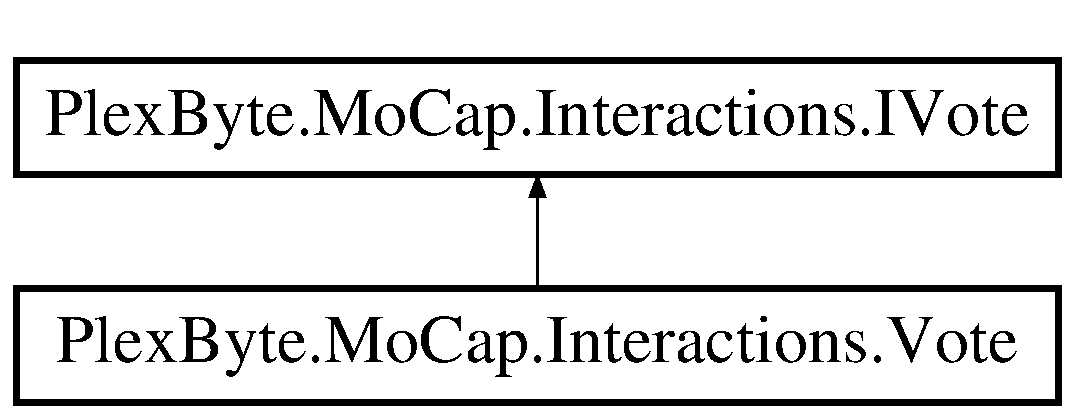
\includegraphics[height=2.000000cm]{interface_plex_byte_1_1_mo_cap_1_1_interactions_1_1_i_vote}
\end{center}
\end{figure}
\subsection*{Properties}
\begin{DoxyCompactItemize}
\item 
I\+User \hyperlink{interface_plex_byte_1_1_mo_cap_1_1_interactions_1_1_i_vote_a9c352cab0ad680e356283c967c3b8a1e}{User}\hspace{0.3cm}{\ttfamily  \mbox{[}get\mbox{]}}
\item 
\hyperlink{interface_plex_byte_1_1_mo_cap_1_1_interactions_1_1_i_survey_option}{I\+Survey\+Option} \hyperlink{interface_plex_byte_1_1_mo_cap_1_1_interactions_1_1_i_vote_afcfbb875e80fb14db21e6880e42984e9}{Option}\hspace{0.3cm}{\ttfamily  \mbox{[}get\mbox{]}}
\item 
Date\+Time \hyperlink{interface_plex_byte_1_1_mo_cap_1_1_interactions_1_1_i_vote_ad249938adad2c0889ca6568ddd9ee577}{Created\+Date\+Time}\hspace{0.3cm}{\ttfamily  \mbox{[}get\mbox{]}}
\item 
string \hyperlink{interface_plex_byte_1_1_mo_cap_1_1_interactions_1_1_i_vote_a72cae3f576897cfb42b46c4206b0fe0f}{Id}\hspace{0.3cm}{\ttfamily  \mbox{[}get\mbox{]}}
\end{DoxyCompactItemize}


\subsection{Detailed Description}
The vote interface 



Definition at line 13 of file I\+Vote.\+cs.



\subsection{Property Documentation}
\index{Plex\+Byte\+::\+Mo\+Cap\+::\+Interactions\+::\+I\+Vote@{Plex\+Byte\+::\+Mo\+Cap\+::\+Interactions\+::\+I\+Vote}!Created\+Date\+Time@{Created\+Date\+Time}}
\index{Created\+Date\+Time@{Created\+Date\+Time}!Plex\+Byte\+::\+Mo\+Cap\+::\+Interactions\+::\+I\+Vote@{Plex\+Byte\+::\+Mo\+Cap\+::\+Interactions\+::\+I\+Vote}}
\subsubsection[{\texorpdfstring{Created\+Date\+Time}{CreatedDateTime}}]{\setlength{\rightskip}{0pt plus 5cm}Date\+Time Plex\+Byte.\+Mo\+Cap.\+Interactions.\+I\+Vote.\+Created\+Date\+Time\hspace{0.3cm}{\ttfamily [get]}}\hypertarget{interface_plex_byte_1_1_mo_cap_1_1_interactions_1_1_i_vote_ad249938adad2c0889ca6568ddd9ee577}{}\label{interface_plex_byte_1_1_mo_cap_1_1_interactions_1_1_i_vote_ad249938adad2c0889ca6568ddd9ee577}


Definition at line 19 of file I\+Vote.\+cs.

\index{Plex\+Byte\+::\+Mo\+Cap\+::\+Interactions\+::\+I\+Vote@{Plex\+Byte\+::\+Mo\+Cap\+::\+Interactions\+::\+I\+Vote}!Id@{Id}}
\index{Id@{Id}!Plex\+Byte\+::\+Mo\+Cap\+::\+Interactions\+::\+I\+Vote@{Plex\+Byte\+::\+Mo\+Cap\+::\+Interactions\+::\+I\+Vote}}
\subsubsection[{\texorpdfstring{Id}{Id}}]{\setlength{\rightskip}{0pt plus 5cm}string Plex\+Byte.\+Mo\+Cap.\+Interactions.\+I\+Vote.\+Id\hspace{0.3cm}{\ttfamily [get]}}\hypertarget{interface_plex_byte_1_1_mo_cap_1_1_interactions_1_1_i_vote_a72cae3f576897cfb42b46c4206b0fe0f}{}\label{interface_plex_byte_1_1_mo_cap_1_1_interactions_1_1_i_vote_a72cae3f576897cfb42b46c4206b0fe0f}


Definition at line 21 of file I\+Vote.\+cs.

\index{Plex\+Byte\+::\+Mo\+Cap\+::\+Interactions\+::\+I\+Vote@{Plex\+Byte\+::\+Mo\+Cap\+::\+Interactions\+::\+I\+Vote}!Option@{Option}}
\index{Option@{Option}!Plex\+Byte\+::\+Mo\+Cap\+::\+Interactions\+::\+I\+Vote@{Plex\+Byte\+::\+Mo\+Cap\+::\+Interactions\+::\+I\+Vote}}
\subsubsection[{\texorpdfstring{Option}{Option}}]{\setlength{\rightskip}{0pt plus 5cm}{\bf I\+Survey\+Option} Plex\+Byte.\+Mo\+Cap.\+Interactions.\+I\+Vote.\+Option\hspace{0.3cm}{\ttfamily [get]}}\hypertarget{interface_plex_byte_1_1_mo_cap_1_1_interactions_1_1_i_vote_afcfbb875e80fb14db21e6880e42984e9}{}\label{interface_plex_byte_1_1_mo_cap_1_1_interactions_1_1_i_vote_afcfbb875e80fb14db21e6880e42984e9}


Definition at line 17 of file I\+Vote.\+cs.

\index{Plex\+Byte\+::\+Mo\+Cap\+::\+Interactions\+::\+I\+Vote@{Plex\+Byte\+::\+Mo\+Cap\+::\+Interactions\+::\+I\+Vote}!User@{User}}
\index{User@{User}!Plex\+Byte\+::\+Mo\+Cap\+::\+Interactions\+::\+I\+Vote@{Plex\+Byte\+::\+Mo\+Cap\+::\+Interactions\+::\+I\+Vote}}
\subsubsection[{\texorpdfstring{User}{User}}]{\setlength{\rightskip}{0pt plus 5cm}I\+User Plex\+Byte.\+Mo\+Cap.\+Interactions.\+I\+Vote.\+User\hspace{0.3cm}{\ttfamily [get]}}\hypertarget{interface_plex_byte_1_1_mo_cap_1_1_interactions_1_1_i_vote_a9c352cab0ad680e356283c967c3b8a1e}{}\label{interface_plex_byte_1_1_mo_cap_1_1_interactions_1_1_i_vote_a9c352cab0ad680e356283c967c3b8a1e}


Definition at line 15 of file I\+Vote.\+cs.



The documentation for this interface was generated from the following file\+:\begin{DoxyCompactItemize}
\item 
D\+:/\+Users/\+Christian\+B/\+Documents/\+\_\+\+H\+F Infomatik/\+Git\+Hub\+\_\+\+Repos/\+Mo\+Cap/\+Plex\+Byte.\+Mo\+Cap/\+Plex\+Byte.\+Mo\+Cap.\+Interactions/\hyperlink{_i_vote_8cs}{I\+Vote.\+cs}\end{DoxyCompactItemize}

\hypertarget{class_plex_byte_1_1_mo_cap_1_1_interactions_1_1_object_factory}{}\section{Plex\+Byte.\+Mo\+Cap.\+Interactions.\+Object\+Factory Class Reference}
\label{class_plex_byte_1_1_mo_cap_1_1_interactions_1_1_object_factory}\index{Plex\+Byte.\+Mo\+Cap.\+Interactions.\+Object\+Factory@{Plex\+Byte.\+Mo\+Cap.\+Interactions.\+Object\+Factory}}
Inheritance diagram for Plex\+Byte.\+Mo\+Cap.\+Interactions.\+Object\+Factory\+:\begin{figure}[H]
\begin{center}
\leavevmode
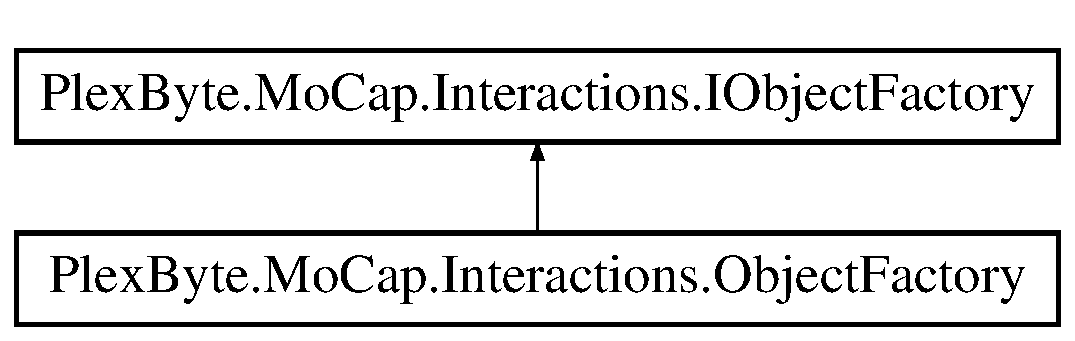
\includegraphics[height=2.000000cm]{class_plex_byte_1_1_mo_cap_1_1_interactions_1_1_object_factory}
\end{center}
\end{figure}
\subsection*{Public Member Functions}
\begin{DoxyCompactItemize}
\item 
virtual \hyperlink{interface_plex_byte_1_1_mo_cap_1_1_interactions_1_1_i_vote}{I\+Vote} \hyperlink{class_plex_byte_1_1_mo_cap_1_1_interactions_1_1_object_factory_a5e26c538cb579f1a31798ce1ae6a4c2f}{Create\+Vote} (string p\+Id, I\+User p\+User, \hyperlink{interface_plex_byte_1_1_mo_cap_1_1_interactions_1_1_i_survey_option}{I\+Survey\+Option} p\+Option)
\item 
virtual \hyperlink{interface_plex_byte_1_1_mo_cap_1_1_interactions_1_1_i_survey_option}{I\+Survey\+Option} \hyperlink{class_plex_byte_1_1_mo_cap_1_1_interactions_1_1_object_factory_ad3a9a100069f91f229baa9bfe1a1205a}{Create\+Survey\+Option} (string p\+Id, string p\+Text)
\item 
virtual I\+User \hyperlink{class_plex_byte_1_1_mo_cap_1_1_interactions_1_1_object_factory_add6cc462c161e617c99f76512fb359dd}{Create\+User} (string p\+Id, string p\+First\+Name, string p\+Last\+Name, string p\+Middle\+Name, string p\+Email, Date\+Time p\+Birthdate, string p\+User\+Name, string p\+Password, Date\+Time p\+Modified, Date\+Time p\+Created, string p\+Person\+Id)
\end{DoxyCompactItemize}


\subsection{Detailed Description}


Definition at line 13 of file Object\+Factory.\+cs.



\subsection{Member Function Documentation}
\index{Plex\+Byte\+::\+Mo\+Cap\+::\+Interactions\+::\+Object\+Factory@{Plex\+Byte\+::\+Mo\+Cap\+::\+Interactions\+::\+Object\+Factory}!Create\+Survey\+Option@{Create\+Survey\+Option}}
\index{Create\+Survey\+Option@{Create\+Survey\+Option}!Plex\+Byte\+::\+Mo\+Cap\+::\+Interactions\+::\+Object\+Factory@{Plex\+Byte\+::\+Mo\+Cap\+::\+Interactions\+::\+Object\+Factory}}
\subsubsection[{\texorpdfstring{Create\+Survey\+Option(string p\+Id, string p\+Text)}{CreateSurveyOption(string pId, string pText)}}]{\setlength{\rightskip}{0pt plus 5cm}virtual {\bf I\+Survey\+Option} Plex\+Byte.\+Mo\+Cap.\+Interactions.\+Object\+Factory.\+Create\+Survey\+Option (
\begin{DoxyParamCaption}
\item[{string}]{p\+Id, }
\item[{string}]{p\+Text}
\end{DoxyParamCaption}
)\hspace{0.3cm}{\ttfamily [virtual]}}\hypertarget{class_plex_byte_1_1_mo_cap_1_1_interactions_1_1_object_factory_ad3a9a100069f91f229baa9bfe1a1205a}{}\label{class_plex_byte_1_1_mo_cap_1_1_interactions_1_1_object_factory_ad3a9a100069f91f229baa9bfe1a1205a}


Implements \hyperlink{interface_plex_byte_1_1_mo_cap_1_1_interactions_1_1_i_object_factory_ad181f2994305f53982828d0d3d8c4621}{Plex\+Byte.\+Mo\+Cap.\+Interactions.\+I\+Object\+Factory}.



Definition at line 22 of file Object\+Factory.\+cs.

\index{Plex\+Byte\+::\+Mo\+Cap\+::\+Interactions\+::\+Object\+Factory@{Plex\+Byte\+::\+Mo\+Cap\+::\+Interactions\+::\+Object\+Factory}!Create\+User@{Create\+User}}
\index{Create\+User@{Create\+User}!Plex\+Byte\+::\+Mo\+Cap\+::\+Interactions\+::\+Object\+Factory@{Plex\+Byte\+::\+Mo\+Cap\+::\+Interactions\+::\+Object\+Factory}}
\subsubsection[{\texorpdfstring{Create\+User(string p\+Id, string p\+First\+Name, string p\+Last\+Name, string p\+Middle\+Name, string p\+Email, Date\+Time p\+Birthdate, string p\+User\+Name, string p\+Password, Date\+Time p\+Modified, Date\+Time p\+Created, string p\+Person\+Id)}{CreateUser(string pId, string pFirstName, string pLastName, string pMiddleName, string pEmail, DateTime pBirthdate, string pUserName, string pPassword, DateTime pModified, DateTime pCreated, string pPersonId)}}]{\setlength{\rightskip}{0pt plus 5cm}virtual I\+User Plex\+Byte.\+Mo\+Cap.\+Interactions.\+Object\+Factory.\+Create\+User (
\begin{DoxyParamCaption}
\item[{string}]{p\+Id, }
\item[{string}]{p\+First\+Name, }
\item[{string}]{p\+Last\+Name, }
\item[{string}]{p\+Middle\+Name, }
\item[{string}]{p\+Email, }
\item[{Date\+Time}]{p\+Birthdate, }
\item[{string}]{p\+User\+Name, }
\item[{string}]{p\+Password, }
\item[{Date\+Time}]{p\+Modified, }
\item[{Date\+Time}]{p\+Created, }
\item[{string}]{p\+Person\+Id}
\end{DoxyParamCaption}
)\hspace{0.3cm}{\ttfamily [virtual]}}\hypertarget{class_plex_byte_1_1_mo_cap_1_1_interactions_1_1_object_factory_add6cc462c161e617c99f76512fb359dd}{}\label{class_plex_byte_1_1_mo_cap_1_1_interactions_1_1_object_factory_add6cc462c161e617c99f76512fb359dd}


Implements \hyperlink{interface_plex_byte_1_1_mo_cap_1_1_interactions_1_1_i_object_factory_ab92eabebbc7307ae04940f46c88b2a30}{Plex\+Byte.\+Mo\+Cap.\+Interactions.\+I\+Object\+Factory}.



Definition at line 29 of file Object\+Factory.\+cs.

\index{Plex\+Byte\+::\+Mo\+Cap\+::\+Interactions\+::\+Object\+Factory@{Plex\+Byte\+::\+Mo\+Cap\+::\+Interactions\+::\+Object\+Factory}!Create\+Vote@{Create\+Vote}}
\index{Create\+Vote@{Create\+Vote}!Plex\+Byte\+::\+Mo\+Cap\+::\+Interactions\+::\+Object\+Factory@{Plex\+Byte\+::\+Mo\+Cap\+::\+Interactions\+::\+Object\+Factory}}
\subsubsection[{\texorpdfstring{Create\+Vote(string p\+Id, I\+User p\+User, I\+Survey\+Option p\+Option)}{CreateVote(string pId, IUser pUser, ISurveyOption pOption)}}]{\setlength{\rightskip}{0pt plus 5cm}virtual {\bf I\+Vote} Plex\+Byte.\+Mo\+Cap.\+Interactions.\+Object\+Factory.\+Create\+Vote (
\begin{DoxyParamCaption}
\item[{string}]{p\+Id, }
\item[{I\+User}]{p\+User, }
\item[{{\bf I\+Survey\+Option}}]{p\+Option}
\end{DoxyParamCaption}
)\hspace{0.3cm}{\ttfamily [virtual]}}\hypertarget{class_plex_byte_1_1_mo_cap_1_1_interactions_1_1_object_factory_a5e26c538cb579f1a31798ce1ae6a4c2f}{}\label{class_plex_byte_1_1_mo_cap_1_1_interactions_1_1_object_factory_a5e26c538cb579f1a31798ce1ae6a4c2f}


Implements \hyperlink{interface_plex_byte_1_1_mo_cap_1_1_interactions_1_1_i_object_factory_ab5ccd5e80e15d76d79504bfe4da715ca}{Plex\+Byte.\+Mo\+Cap.\+Interactions.\+I\+Object\+Factory}.



Definition at line 15 of file Object\+Factory.\+cs.



The documentation for this class was generated from the following file\+:\begin{DoxyCompactItemize}
\item 
D\+:/\+Users/\+Christian\+B/\+Documents/\+\_\+\+H\+F Infomatik/\+Git\+Hub\+\_\+\+Repos/\+Mo\+Cap/\+Plex\+Byte.\+Mo\+Cap/\+Plex\+Byte.\+Mo\+Cap.\+Interactions/\hyperlink{_object_factory_8cs}{Object\+Factory.\+cs}\end{DoxyCompactItemize}

\hypertarget{class_plex_byte_1_1_mo_cap_1_1_interactions_1_1_project}{}\section{Plex\+Byte.\+Mo\+Cap.\+Interactions.\+Project Class Reference}
\label{class_plex_byte_1_1_mo_cap_1_1_interactions_1_1_project}\index{Plex\+Byte.\+Mo\+Cap.\+Interactions.\+Project@{Plex\+Byte.\+Mo\+Cap.\+Interactions.\+Project}}
Inheritance diagram for Plex\+Byte.\+Mo\+Cap.\+Interactions.\+Project\+:\begin{figure}[H]
\begin{center}
\leavevmode
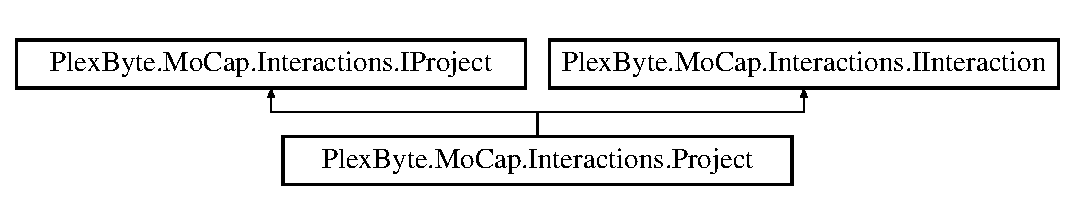
\includegraphics[height=2.000000cm]{class_plex_byte_1_1_mo_cap_1_1_interactions_1_1_project}
\end{center}
\end{figure}
\subsection*{Public Member Functions}
\begin{DoxyCompactItemize}
\item 
\hyperlink{class_plex_byte_1_1_mo_cap_1_1_interactions_1_1_project_a74a8da786a74fd3765139ef88034671c}{Project} (string p\+Id, string p\+Text, bool p\+Enable\+Balance, bool p\+Enable\+Survey, Date\+Time p\+Start\+Dt, Date\+Time p\+End\+Dt, I\+User p\+Creator)
\begin{DoxyCompactList}\small\item\em Constructor of the class \end{DoxyCompactList}\item 
\hyperlink{class_plex_byte_1_1_mo_cap_1_1_interactions_1_1_project_aee7a878c58675b85315590eebc17f654}{Project} (string p\+Id, string p\+Name, string p\+Text, bool p\+Enable\+Balance, bool p\+Enable\+Survey, Date\+Time p\+Start\+Dt, Date\+Time p\+End\+Dt, I\+User p\+Creator, I\+User p\+Owner, List$<$ I\+User $>$ p\+Member\+List, List$<$ I\+User $>$ p\+Invitation\+List, List$<$ \hyperlink{interface_plex_byte_1_1_mo_cap_1_1_interactions_1_1_i_task}{I\+Task} $>$ p\+Task\+List, List$<$ \hyperlink{interface_plex_byte_1_1_mo_cap_1_1_interactions_1_1_i_survey}{I\+Survey} $>$ p\+Survey\+List)
\begin{DoxyCompactList}\small\item\em Constructor of the class \end{DoxyCompactList}\item 
virtual void \hyperlink{class_plex_byte_1_1_mo_cap_1_1_interactions_1_1_project_a039fdf13ac3d4b2b83cb0f3ce7fb4ca1}{On\+Complete} (\hyperlink{class_plex_byte_1_1_mo_cap_1_1_interactions_1_1_interaction_event_args}{Interaction\+Event\+Args} p\+Event\+Args)
\begin{DoxyCompactList}\small\item\em This method raises the corresponding event in case subscribers are registered \end{DoxyCompactList}\item 
virtual void \hyperlink{class_plex_byte_1_1_mo_cap_1_1_interactions_1_1_project_a3255cca2b9dbe1fc60a39463d33a9c31}{On\+Modify} (\hyperlink{class_plex_byte_1_1_mo_cap_1_1_interactions_1_1_interaction_event_args}{Interaction\+Event\+Args} p\+Event\+Args)
\begin{DoxyCompactList}\small\item\em This method raises the corresponding event in case subscribers are registered \end{DoxyCompactList}\item 
virtual void \hyperlink{class_plex_byte_1_1_mo_cap_1_1_interactions_1_1_project_ad08e79e01889284723d1dda27a3fb9c8}{On\+State\+Changed} (\hyperlink{class_plex_byte_1_1_mo_cap_1_1_interactions_1_1_interaction_event_args}{Interaction\+Event\+Args} p\+Event\+Args)
\begin{DoxyCompactList}\small\item\em This method raises the corresponding event in case subscribers are registered \end{DoxyCompactList}\item 
virtual void \hyperlink{class_plex_byte_1_1_mo_cap_1_1_interactions_1_1_project_a0c145698f05dc44311f8a9f819a4d57a}{On\+User\+Add} (\hyperlink{class_plex_byte_1_1_mo_cap_1_1_interactions_1_1_interaction_event_args}{Interaction\+Event\+Args} p\+Event\+Args)
\begin{DoxyCompactList}\small\item\em This method raises the corresponding event in case subscribers are registered \end{DoxyCompactList}\item 
virtual void \hyperlink{class_plex_byte_1_1_mo_cap_1_1_interactions_1_1_project_ac55a17f8dec4f7319f08c8e05a28ae81}{On\+User\+Ban} (\hyperlink{class_plex_byte_1_1_mo_cap_1_1_interactions_1_1_interaction_event_args}{Interaction\+Event\+Args} p\+Event\+Args)
\begin{DoxyCompactList}\small\item\em This method raises the corresponding event in case subscribers are registered \end{DoxyCompactList}\item 
virtual void \hyperlink{class_plex_byte_1_1_mo_cap_1_1_interactions_1_1_project_ac6cbff0fad9543c37a22e52ad23d7ebd}{On\+Leave} (\hyperlink{class_plex_byte_1_1_mo_cap_1_1_interactions_1_1_interaction_event_args}{Interaction\+Event\+Args} p\+Event\+Args)
\begin{DoxyCompactList}\small\item\em This method raises the corresponding event in case subscribers are registered \end{DoxyCompactList}\item 
virtual void \hyperlink{class_plex_byte_1_1_mo_cap_1_1_interactions_1_1_project_a62c49cc0097eefd5ba3c070585a9a5a4}{On\+User\+Invite} (\hyperlink{class_plex_byte_1_1_mo_cap_1_1_interactions_1_1_interaction_event_args}{Interaction\+Event\+Args} p\+Event\+Args)
\begin{DoxyCompactList}\small\item\em This method raises the corresponding event in case subscribers are registered \end{DoxyCompactList}\item 
virtual void \hyperlink{class_plex_byte_1_1_mo_cap_1_1_interactions_1_1_project_a70de0ac1540fa8d7eec9292379d83d0c}{On\+Task\+Add} (\hyperlink{class_plex_byte_1_1_mo_cap_1_1_interactions_1_1_interaction_event_args}{Interaction\+Event\+Args} p\+Event\+Args)
\begin{DoxyCompactList}\small\item\em This method raises the corresponding event in case subscribers are registered \end{DoxyCompactList}\item 
virtual void \hyperlink{class_plex_byte_1_1_mo_cap_1_1_interactions_1_1_project_a464040e9abe13cc8d09e71bedb81a1c2}{On\+Survey\+Add} (\hyperlink{class_plex_byte_1_1_mo_cap_1_1_interactions_1_1_interaction_event_args}{Interaction\+Event\+Args} p\+Event\+Args)
\begin{DoxyCompactList}\small\item\em This method raises the corresponding event in case subscribers are registered \end{DoxyCompactList}\item 
virtual void \hyperlink{class_plex_byte_1_1_mo_cap_1_1_interactions_1_1_project_a4e59d6c532937fb758e055af3fa2da77}{Change\+Owner} (I\+User p\+User)
\begin{DoxyCompactList}\small\item\em This method changes the owner of the project and raises the modified event if the owner is different used to create a secound project-\/admin \end{DoxyCompactList}\item 
virtual void \hyperlink{class_plex_byte_1_1_mo_cap_1_1_interactions_1_1_project_adcbdd39b8b64051e9bbdfffd25663116}{Change\+Is\+Active} (bool p\+Active)
\begin{DoxyCompactList}\small\item\em This method changes the active flag of the object. This can occure if the item expired, finished or was cancelled. It will raise the Modified event once changed \end{DoxyCompactList}\item 
virtual void \hyperlink{class_plex_byte_1_1_mo_cap_1_1_interactions_1_1_project_a4d3d0c6c63e3dc3162ec2f5a314bade1}{Add\+Task} (\hyperlink{interface_plex_byte_1_1_mo_cap_1_1_interactions_1_1_i_task}{I\+Task} p\+Task)
\begin{DoxyCompactList}\small\item\em This method adds a \hyperlink{class_plex_byte_1_1_mo_cap_1_1_interactions_1_1_task}{Task} to the list of tasks from the project \end{DoxyCompactList}\item 
virtual void \hyperlink{class_plex_byte_1_1_mo_cap_1_1_interactions_1_1_project_af374761c89f59d42b1a79fdb5cf0311d}{Add\+Survey} (\hyperlink{interface_plex_byte_1_1_mo_cap_1_1_interactions_1_1_i_survey}{I\+Survey} p\+Survey)
\begin{DoxyCompactList}\small\item\em This method adds a \hyperlink{class_plex_byte_1_1_mo_cap_1_1_interactions_1_1_survey}{Survey} to the list of surveys from the project \end{DoxyCompactList}\item 
virtual void \hyperlink{class_plex_byte_1_1_mo_cap_1_1_interactions_1_1_project_a44b3e36d693cffce67d606f2f040927e}{Invite} (I\+User p\+User)
\begin{DoxyCompactList}\small\item\em To invite a user to a projec, it adds the user to the invitations list \end{DoxyCompactList}\item 
virtual void \hyperlink{class_plex_byte_1_1_mo_cap_1_1_interactions_1_1_project_a06b884b97b543b4c8ba64993e4008a6f}{Accept} (I\+User p\+User)
\begin{DoxyCompactList}\small\item\em After a user is invited to a project this method removes the user from the invitation list and adds the same to the member list \end{DoxyCompactList}\item 
virtual void \hyperlink{class_plex_byte_1_1_mo_cap_1_1_interactions_1_1_project_a12152d11fc38eedc1b93dd56ee73f42c}{Leave} (I\+User p\+User)
\begin{DoxyCompactList}\small\item\em Removes oneself from the memberlist of the project \end{DoxyCompactList}\item 
virtual void \hyperlink{class_plex_byte_1_1_mo_cap_1_1_interactions_1_1_project_a0fe352bded53612ae6e23859b0ce8802}{Kick\+User} (I\+User p\+User)
\begin{DoxyCompactList}\small\item\em Kicks a user from the project. It removes a user from the memberlist \end{DoxyCompactList}\item 
virtual void \hyperlink{class_plex_byte_1_1_mo_cap_1_1_interactions_1_1_project_a7a916aeebe04d4dd33765b6127282543}{Change\+State} (\hyperlink{namespace_plex_byte_1_1_mo_cap_1_1_interactions_afcb673d9186608b6bd3b187179aedc8a}{Interaction\+State} p\+State)
\begin{DoxyCompactList}\small\item\em Changes the state of this interaction and thus causes the state\+Changed event to be fired \end{DoxyCompactList}\end{DoxyCompactItemize}
\subsection*{Properties}
\begin{DoxyCompactItemize}
\item 
string \hyperlink{class_plex_byte_1_1_mo_cap_1_1_interactions_1_1_project_ad78c8f3d9736e6c9dccb1d0e0a0748f7}{Id}\hspace{0.3cm}{\ttfamily  \mbox{[}get\mbox{]}}
\begin{DoxyCompactList}\small\item\em The unique id of the project \end{DoxyCompactList}\item 
Date\+Time \hyperlink{class_plex_byte_1_1_mo_cap_1_1_interactions_1_1_project_ab1d85e04faa4f114a466abf8f238b7d5}{Start\+Date\+Time}\hspace{0.3cm}{\ttfamily  \mbox{[}get, set\mbox{]}}
\begin{DoxyCompactList}\small\item\em The date and time this project becomes active and can be worked on. As long as this date is not reached the state will remain queued and no work can be performed on the project as longs as it is in state queued \end{DoxyCompactList}\item 
Date\+Time \hyperlink{class_plex_byte_1_1_mo_cap_1_1_interactions_1_1_project_a12da623278dc598539d16694aab4f136}{End\+Date\+Time}\hspace{0.3cm}{\ttfamily  \mbox{[}get, set\mbox{]}}
\begin{DoxyCompactList}\small\item\em The date and time this project should be finished. If this date is reached the state will change to expired \end{DoxyCompactList}\item 
Date\+Time \hyperlink{class_plex_byte_1_1_mo_cap_1_1_interactions_1_1_project_a9d79cd9f19fef0e610933a19e5cdc099}{Created\+Date\+Time}\hspace{0.3cm}{\ttfamily  \mbox{[}get\mbox{]}}
\begin{DoxyCompactList}\small\item\em The date and time the project was created \end{DoxyCompactList}\item 
Date\+Time \hyperlink{class_plex_byte_1_1_mo_cap_1_1_interactions_1_1_project_a5f3569713936103ba32da4338094a787}{Modified\+Date\+Time}\hspace{0.3cm}{\ttfamily  \mbox{[}get, set\mbox{]}}
\begin{DoxyCompactList}\small\item\em The date and time the project was last modified \end{DoxyCompactList}\item 
bool \hyperlink{class_plex_byte_1_1_mo_cap_1_1_interactions_1_1_project_ac9b00a5a3ce25337a513dfc9c1f6a380}{Is\+Active}\hspace{0.3cm}{\ttfamily  \mbox{[}get\mbox{]}}
\begin{DoxyCompactList}\small\item\em Flag indicating whether or not the project can be worked on \end{DoxyCompactList}\item 
string \hyperlink{class_plex_byte_1_1_mo_cap_1_1_interactions_1_1_project_aaa6c4ef85c6ebc943137fdc24705715c}{Text}\hspace{0.3cm}{\ttfamily  \mbox{[}get, set\mbox{]}}
\begin{DoxyCompactList}\small\item\em The text of this project (description) \end{DoxyCompactList}\item 
\hyperlink{namespace_plex_byte_1_1_mo_cap_1_1_interactions_a6e7bea333446664bbce2bb296db25e31}{Interaction\+Type} \hyperlink{class_plex_byte_1_1_mo_cap_1_1_interactions_1_1_project_aea479ae8fe5363b41c132933c6fb6e4a}{Type}\hspace{0.3cm}{\ttfamily  \mbox{[}get\mbox{]}}
\begin{DoxyCompactList}\small\item\em The type of interaction (will be always project) \end{DoxyCompactList}\item 
I\+User \hyperlink{class_plex_byte_1_1_mo_cap_1_1_interactions_1_1_project_aa121bc39de6d60290903f188a3734557}{Creator} = \hyperlink{namespace_plex_byte_1_1_mo_cap_1_1_interactions_a6e7bea333446664bbce2bb296db25e31a9e727fdd3aec8274f46685441900280d}{Interaction\+Type.\+Project}\hspace{0.3cm}{\ttfamily  \mbox{[}get\mbox{]}}
\begin{DoxyCompactList}\small\item\em The user that created the project \end{DoxyCompactList}\item 
I\+User \hyperlink{class_plex_byte_1_1_mo_cap_1_1_interactions_1_1_project_adf1484b6a6103c1c2104f6dfbba9eace}{Owner}\hspace{0.3cm}{\ttfamily  \mbox{[}get, set\mbox{]}}
\begin{DoxyCompactList}\small\item\em The user currently owning the project \end{DoxyCompactList}\item 
\hyperlink{namespace_plex_byte_1_1_mo_cap_1_1_interactions_afcb673d9186608b6bd3b187179aedc8a}{Interaction\+State} \hyperlink{class_plex_byte_1_1_mo_cap_1_1_interactions_1_1_project_ae322c2cd5f5b5a080c6f6f17badeaa2b}{State}\hspace{0.3cm}{\ttfamily  \mbox{[}get\mbox{]}}
\begin{DoxyCompactList}\small\item\em The state of the project \end{DoxyCompactList}\item 
bool \hyperlink{class_plex_byte_1_1_mo_cap_1_1_interactions_1_1_project_a416293f2e592d5d42afecdd3a4f99737}{Enable\+Balance}\hspace{0.3cm}{\ttfamily  \mbox{[}get\mbox{]}}
\begin{DoxyCompactList}\small\item\em A bool to set, if it is possible to set a balance to a project if disabled it is not possible to book spended time or effort in a project \end{DoxyCompactList}\item 
bool \hyperlink{class_plex_byte_1_1_mo_cap_1_1_interactions_1_1_project_a38db02bda9f7cb2d264dbc890da9321a}{Enable\+Survey}\hspace{0.3cm}{\ttfamily  \mbox{[}get\mbox{]}}
\begin{DoxyCompactList}\small\item\em A bool to set, if it is possible to set up a survey to a project if disabled it is not possible to create one \end{DoxyCompactList}\item 
\hyperlink{interface_plex_byte_1_1_mo_cap_1_1_interactions_1_1_i_account}{I\+Account} \hyperlink{class_plex_byte_1_1_mo_cap_1_1_interactions_1_1_project_a453929da12473119b7d1d4bd21e986c4}{Project\+Account}\hspace{0.3cm}{\ttfamily  \mbox{[}get, set\mbox{]}}
\begin{DoxyCompactList}\small\item\em The account which is conectet do the project \end{DoxyCompactList}\item 
List$<$ I\+User $>$ \hyperlink{class_plex_byte_1_1_mo_cap_1_1_interactions_1_1_project_afedd69d0ca0662b9c1b03431339b129d}{Invitation\+List}\hspace{0.3cm}{\ttfamily  \mbox{[}get\mbox{]}}
\begin{DoxyCompactList}\small\item\em In this list are all members which have to answer an invitation \end{DoxyCompactList}\item 
List$<$ \hyperlink{interface_plex_byte_1_1_mo_cap_1_1_interactions_1_1_i_task}{I\+Task} $>$ \hyperlink{class_plex_byte_1_1_mo_cap_1_1_interactions_1_1_project_ab55a7377ee7124ba1af72ac486db8953}{Task\+List}\hspace{0.3cm}{\ttfamily  \mbox{[}get\mbox{]}}
\begin{DoxyCompactList}\small\item\em A list of all tasks in a project \end{DoxyCompactList}\item 
List$<$ \hyperlink{interface_plex_byte_1_1_mo_cap_1_1_interactions_1_1_i_survey}{I\+Survey} $>$ \hyperlink{class_plex_byte_1_1_mo_cap_1_1_interactions_1_1_project_aeafe2719337840a5afb37d431db20639}{Survey\+List}\hspace{0.3cm}{\ttfamily  \mbox{[}get\mbox{]}}
\begin{DoxyCompactList}\small\item\em A list of all surveys in a project \end{DoxyCompactList}\item 
List$<$ I\+User $>$ \hyperlink{class_plex_byte_1_1_mo_cap_1_1_interactions_1_1_project_a2b3c3d78367b1ca4f4a4ae87e3b444ab}{Member\+List}\hspace{0.3cm}{\ttfamily  \mbox{[}get\mbox{]}}
\begin{DoxyCompactList}\small\item\em In this list are all members of a project \end{DoxyCompactList}\item 
string \hyperlink{class_plex_byte_1_1_mo_cap_1_1_interactions_1_1_project_aa6a59b416e07515e6d8799f410157488}{Name}\hspace{0.3cm}{\ttfamily  \mbox{[}get, set\mbox{]}}
\begin{DoxyCompactList}\small\item\em The name of the project \end{DoxyCompactList}\end{DoxyCompactItemize}
\subsection*{Events}
\begin{DoxyCompactItemize}
\item 
\hyperlink{namespace_plex_byte_1_1_mo_cap_1_1_interactions_ac81ac3321ab2b018c75ad2c18ec15b9e}{Complete} \hyperlink{class_plex_byte_1_1_mo_cap_1_1_interactions_1_1_project_a4ee1861f64f1fdc8092854c2d9c26ea0}{Completed}
\item 
\hyperlink{namespace_plex_byte_1_1_mo_cap_1_1_interactions_a490186f613e46adce26244f3b2c78a58}{Modify} \hyperlink{class_plex_byte_1_1_mo_cap_1_1_interactions_1_1_project_a437ba816061b8662712a82580618e4c7}{Modified}
\item 
\hyperlink{namespace_plex_byte_1_1_mo_cap_1_1_interactions_af2ff213e81451f96fc74bfad114cecde}{State\+Change} \hyperlink{class_plex_byte_1_1_mo_cap_1_1_interactions_1_1_project_a79227b0122133a9c437832f7fc24b3d4}{State\+Changed}
\item 
\hyperlink{namespace_plex_byte_1_1_mo_cap_1_1_interactions_a16841bb191709e7941fc1acb4d96f24f}{User\+Add} \hyperlink{class_plex_byte_1_1_mo_cap_1_1_interactions_1_1_project_a592cd80361adb23a54880c8de56c6f65}{User\+Added}
\item 
\hyperlink{namespace_plex_byte_1_1_mo_cap_1_1_interactions_a7dea125552945356069febe97eb72332}{User\+Ban} \hyperlink{class_plex_byte_1_1_mo_cap_1_1_interactions_1_1_project_a751af6b596331db773b28fa6e7b8c22f}{User\+Banned}
\item 
\hyperlink{class_plex_byte_1_1_mo_cap_1_1_interactions_1_1_project_a12152d11fc38eedc1b93dd56ee73f42c}{Leave} \hyperlink{class_plex_byte_1_1_mo_cap_1_1_interactions_1_1_project_a385ca7e4f05b1dba7c270ed935fe73d3}{Left}
\item 
\hyperlink{namespace_plex_byte_1_1_mo_cap_1_1_interactions_aef92e5d1e9d0a246188e890e95317f08}{User\+Invite} \hyperlink{class_plex_byte_1_1_mo_cap_1_1_interactions_1_1_project_a43bd9aced645c1a0fe86e3608a524c18}{User\+Invited}
\item 
\hyperlink{namespace_plex_byte_1_1_mo_cap_1_1_interactions_a15d0878ea4e4b99061b0424143eb2ce5}{Task\+Add} \hyperlink{class_plex_byte_1_1_mo_cap_1_1_interactions_1_1_project_a084eca4bac34679e2a56cb50e4ffd20f}{Task\+Added}
\item 
\hyperlink{namespace_plex_byte_1_1_mo_cap_1_1_interactions_a1900501fc00150a42afd117937b7e88e}{Survey\+Add} \hyperlink{class_plex_byte_1_1_mo_cap_1_1_interactions_1_1_project_aff8992fdcc8b6ee532e38f1f474cb0f1}{Survey\+Added}
\end{DoxyCompactItemize}


\subsection{Detailed Description}


Definition at line 11 of file Project.\+cs.



\subsection{Constructor \& Destructor Documentation}
\index{Plex\+Byte\+::\+Mo\+Cap\+::\+Interactions\+::\+Project@{Plex\+Byte\+::\+Mo\+Cap\+::\+Interactions\+::\+Project}!Project@{Project}}
\index{Project@{Project}!Plex\+Byte\+::\+Mo\+Cap\+::\+Interactions\+::\+Project@{Plex\+Byte\+::\+Mo\+Cap\+::\+Interactions\+::\+Project}}
\subsubsection[{\texorpdfstring{Project(string p\+Id, string p\+Text, bool p\+Enable\+Balance, bool p\+Enable\+Survey, Date\+Time p\+Start\+Dt, Date\+Time p\+End\+Dt, I\+User p\+Creator)}{Project(string pId, string pText, bool pEnableBalance, bool pEnableSurvey, DateTime pStartDt, DateTime pEndDt, IUser pCreator)}}]{\setlength{\rightskip}{0pt plus 5cm}Plex\+Byte.\+Mo\+Cap.\+Interactions.\+Project.\+Project (
\begin{DoxyParamCaption}
\item[{string}]{p\+Id, }
\item[{string}]{p\+Text, }
\item[{bool}]{p\+Enable\+Balance, }
\item[{bool}]{p\+Enable\+Survey, }
\item[{Date\+Time}]{p\+Start\+Dt, }
\item[{Date\+Time}]{p\+End\+Dt, }
\item[{I\+User}]{p\+Creator}
\end{DoxyParamCaption}
)}\hypertarget{class_plex_byte_1_1_mo_cap_1_1_interactions_1_1_project_a74a8da786a74fd3765139ef88034671c}{}\label{class_plex_byte_1_1_mo_cap_1_1_interactions_1_1_project_a74a8da786a74fd3765139ef88034671c}


Constructor of the class 


\begin{DoxyParams}{Parameters}
{\em p\+Id} & \\
\hline
{\em p\+Text} & \\
\hline
{\em p\+Enable\+Balance} & \\
\hline
{\em p\+Enable\+Survey} & \\
\hline
{\em p\+Creator} & \\
\hline
\end{DoxyParams}


Definition at line 131 of file Project.\+cs.

\index{Plex\+Byte\+::\+Mo\+Cap\+::\+Interactions\+::\+Project@{Plex\+Byte\+::\+Mo\+Cap\+::\+Interactions\+::\+Project}!Project@{Project}}
\index{Project@{Project}!Plex\+Byte\+::\+Mo\+Cap\+::\+Interactions\+::\+Project@{Plex\+Byte\+::\+Mo\+Cap\+::\+Interactions\+::\+Project}}
\subsubsection[{\texorpdfstring{Project(string p\+Id, string p\+Name, string p\+Text, bool p\+Enable\+Balance, bool p\+Enable\+Survey, Date\+Time p\+Start\+Dt, Date\+Time p\+End\+Dt, I\+User p\+Creator, I\+User p\+Owner, List$<$ I\+User $>$ p\+Member\+List, List$<$ I\+User $>$ p\+Invitation\+List, List$<$ I\+Task $>$ p\+Task\+List, List$<$ I\+Survey $>$ p\+Survey\+List)}{Project(string pId, string pName, string pText, bool pEnableBalance, bool pEnableSurvey, DateTime pStartDt, DateTime pEndDt, IUser pCreator, IUser pOwner, List< IUser > pMemberList, List< IUser > pInvitationList, List< ITask > pTaskList, List< ISurvey > pSurveyList)}}]{\setlength{\rightskip}{0pt plus 5cm}Plex\+Byte.\+Mo\+Cap.\+Interactions.\+Project.\+Project (
\begin{DoxyParamCaption}
\item[{string}]{p\+Id, }
\item[{string}]{p\+Name, }
\item[{string}]{p\+Text, }
\item[{bool}]{p\+Enable\+Balance, }
\item[{bool}]{p\+Enable\+Survey, }
\item[{Date\+Time}]{p\+Start\+Dt, }
\item[{Date\+Time}]{p\+End\+Dt, }
\item[{I\+User}]{p\+Creator, }
\item[{I\+User}]{p\+Owner, }
\item[{List$<$ I\+User $>$}]{p\+Member\+List, }
\item[{List$<$ I\+User $>$}]{p\+Invitation\+List, }
\item[{List$<$ {\bf I\+Task} $>$}]{p\+Task\+List, }
\item[{List$<$ {\bf I\+Survey} $>$}]{p\+Survey\+List}
\end{DoxyParamCaption}
)}\hypertarget{class_plex_byte_1_1_mo_cap_1_1_interactions_1_1_project_aee7a878c58675b85315590eebc17f654}{}\label{class_plex_byte_1_1_mo_cap_1_1_interactions_1_1_project_aee7a878c58675b85315590eebc17f654}


Constructor of the class 


\begin{DoxyParams}{Parameters}
{\em p\+Id} & \\
\hline
{\em p\+Text} & \\
\hline
{\em p\+Enable\+Balance} & \\
\hline
{\em p\+Enable\+Survey} & \\
\hline
{\em p\+Member\+List} & \\
\hline
{\em p\+Invitation\+List} & \\
\hline
{\em p\+Task\+List} & \\
\hline
{\em p\+Survey\+List} & \\
\hline
{\em p\+Creator} & \\
\hline
{\em p\+Owner} & \\
\hline
\end{DoxyParams}


Definition at line 155 of file Project.\+cs.



\subsection{Member Function Documentation}
\index{Plex\+Byte\+::\+Mo\+Cap\+::\+Interactions\+::\+Project@{Plex\+Byte\+::\+Mo\+Cap\+::\+Interactions\+::\+Project}!Accept@{Accept}}
\index{Accept@{Accept}!Plex\+Byte\+::\+Mo\+Cap\+::\+Interactions\+::\+Project@{Plex\+Byte\+::\+Mo\+Cap\+::\+Interactions\+::\+Project}}
\subsubsection[{\texorpdfstring{Accept(\+I\+User p\+User)}{Accept(IUser pUser)}}]{\setlength{\rightskip}{0pt plus 5cm}virtual void Plex\+Byte.\+Mo\+Cap.\+Interactions.\+Project.\+Accept (
\begin{DoxyParamCaption}
\item[{I\+User}]{p\+User}
\end{DoxyParamCaption}
)\hspace{0.3cm}{\ttfamily [virtual]}}\hypertarget{class_plex_byte_1_1_mo_cap_1_1_interactions_1_1_project_a06b884b97b543b4c8ba64993e4008a6f}{}\label{class_plex_byte_1_1_mo_cap_1_1_interactions_1_1_project_a06b884b97b543b4c8ba64993e4008a6f}


After a user is invited to a project this method removes the user from the invitation list and adds the same to the member list 


\begin{DoxyParams}{Parameters}
{\em p\+User} & \\
\hline
\end{DoxyParams}


Implements \hyperlink{interface_plex_byte_1_1_mo_cap_1_1_interactions_1_1_i_project_ab3bcc21a56e10b5e44381fe133420f71}{Plex\+Byte.\+Mo\+Cap.\+Interactions.\+I\+Project}.



Definition at line 319 of file Project.\+cs.

\index{Plex\+Byte\+::\+Mo\+Cap\+::\+Interactions\+::\+Project@{Plex\+Byte\+::\+Mo\+Cap\+::\+Interactions\+::\+Project}!Add\+Survey@{Add\+Survey}}
\index{Add\+Survey@{Add\+Survey}!Plex\+Byte\+::\+Mo\+Cap\+::\+Interactions\+::\+Project@{Plex\+Byte\+::\+Mo\+Cap\+::\+Interactions\+::\+Project}}
\subsubsection[{\texorpdfstring{Add\+Survey(\+I\+Survey p\+Survey)}{AddSurvey(ISurvey pSurvey)}}]{\setlength{\rightskip}{0pt plus 5cm}virtual void Plex\+Byte.\+Mo\+Cap.\+Interactions.\+Project.\+Add\+Survey (
\begin{DoxyParamCaption}
\item[{{\bf I\+Survey}}]{p\+Survey}
\end{DoxyParamCaption}
)\hspace{0.3cm}{\ttfamily [virtual]}}\hypertarget{class_plex_byte_1_1_mo_cap_1_1_interactions_1_1_project_af374761c89f59d42b1a79fdb5cf0311d}{}\label{class_plex_byte_1_1_mo_cap_1_1_interactions_1_1_project_af374761c89f59d42b1a79fdb5cf0311d}


This method adds a \hyperlink{class_plex_byte_1_1_mo_cap_1_1_interactions_1_1_survey}{Survey} to the list of surveys from the project 


\begin{DoxyParams}{Parameters}
{\em p\+Survey} & \\
\hline
\end{DoxyParams}


Implements \hyperlink{interface_plex_byte_1_1_mo_cap_1_1_interactions_1_1_i_project_abd866426be16a3223f4930f6501e7114}{Plex\+Byte.\+Mo\+Cap.\+Interactions.\+I\+Project}.



Definition at line 292 of file Project.\+cs.

\index{Plex\+Byte\+::\+Mo\+Cap\+::\+Interactions\+::\+Project@{Plex\+Byte\+::\+Mo\+Cap\+::\+Interactions\+::\+Project}!Add\+Task@{Add\+Task}}
\index{Add\+Task@{Add\+Task}!Plex\+Byte\+::\+Mo\+Cap\+::\+Interactions\+::\+Project@{Plex\+Byte\+::\+Mo\+Cap\+::\+Interactions\+::\+Project}}
\subsubsection[{\texorpdfstring{Add\+Task(\+I\+Task p\+Task)}{AddTask(ITask pTask)}}]{\setlength{\rightskip}{0pt plus 5cm}virtual void Plex\+Byte.\+Mo\+Cap.\+Interactions.\+Project.\+Add\+Task (
\begin{DoxyParamCaption}
\item[{{\bf I\+Task}}]{p\+Task}
\end{DoxyParamCaption}
)\hspace{0.3cm}{\ttfamily [virtual]}}\hypertarget{class_plex_byte_1_1_mo_cap_1_1_interactions_1_1_project_a4d3d0c6c63e3dc3162ec2f5a314bade1}{}\label{class_plex_byte_1_1_mo_cap_1_1_interactions_1_1_project_a4d3d0c6c63e3dc3162ec2f5a314bade1}


This method adds a \hyperlink{class_plex_byte_1_1_mo_cap_1_1_interactions_1_1_task}{Task} to the list of tasks from the project 


\begin{DoxyParams}{Parameters}
{\em p\+Task} & \\
\hline
\end{DoxyParams}


Implements \hyperlink{interface_plex_byte_1_1_mo_cap_1_1_interactions_1_1_i_project_a9ce2ef4ee8b2d18da93405ea42113980}{Plex\+Byte.\+Mo\+Cap.\+Interactions.\+I\+Project}.



Definition at line 280 of file Project.\+cs.

\index{Plex\+Byte\+::\+Mo\+Cap\+::\+Interactions\+::\+Project@{Plex\+Byte\+::\+Mo\+Cap\+::\+Interactions\+::\+Project}!Change\+Is\+Active@{Change\+Is\+Active}}
\index{Change\+Is\+Active@{Change\+Is\+Active}!Plex\+Byte\+::\+Mo\+Cap\+::\+Interactions\+::\+Project@{Plex\+Byte\+::\+Mo\+Cap\+::\+Interactions\+::\+Project}}
\subsubsection[{\texorpdfstring{Change\+Is\+Active(bool p\+Active)}{ChangeIsActive(bool pActive)}}]{\setlength{\rightskip}{0pt plus 5cm}virtual void Plex\+Byte.\+Mo\+Cap.\+Interactions.\+Project.\+Change\+Is\+Active (
\begin{DoxyParamCaption}
\item[{bool}]{p\+Active}
\end{DoxyParamCaption}
)\hspace{0.3cm}{\ttfamily [virtual]}}\hypertarget{class_plex_byte_1_1_mo_cap_1_1_interactions_1_1_project_adcbdd39b8b64051e9bbdfffd25663116}{}\label{class_plex_byte_1_1_mo_cap_1_1_interactions_1_1_project_adcbdd39b8b64051e9bbdfffd25663116}


This method changes the active flag of the object. This can occure if the item expired, finished or was cancelled. It will raise the Modified event once changed 


\begin{DoxyParams}{Parameters}
{\em p\+Active} & \\
\hline
\end{DoxyParams}


Implements \hyperlink{interface_plex_byte_1_1_mo_cap_1_1_interactions_1_1_i_interaction_ac2d9f47a1139b931939e8cff07153aba}{Plex\+Byte.\+Mo\+Cap.\+Interactions.\+I\+Interaction}.



Definition at line 266 of file Project.\+cs.

\index{Plex\+Byte\+::\+Mo\+Cap\+::\+Interactions\+::\+Project@{Plex\+Byte\+::\+Mo\+Cap\+::\+Interactions\+::\+Project}!Change\+Owner@{Change\+Owner}}
\index{Change\+Owner@{Change\+Owner}!Plex\+Byte\+::\+Mo\+Cap\+::\+Interactions\+::\+Project@{Plex\+Byte\+::\+Mo\+Cap\+::\+Interactions\+::\+Project}}
\subsubsection[{\texorpdfstring{Change\+Owner(\+I\+User p\+User)}{ChangeOwner(IUser pUser)}}]{\setlength{\rightskip}{0pt plus 5cm}virtual void Plex\+Byte.\+Mo\+Cap.\+Interactions.\+Project.\+Change\+Owner (
\begin{DoxyParamCaption}
\item[{I\+User}]{p\+User}
\end{DoxyParamCaption}
)\hspace{0.3cm}{\ttfamily [virtual]}}\hypertarget{class_plex_byte_1_1_mo_cap_1_1_interactions_1_1_project_a4e59d6c532937fb758e055af3fa2da77}{}\label{class_plex_byte_1_1_mo_cap_1_1_interactions_1_1_project_a4e59d6c532937fb758e055af3fa2da77}


This method changes the owner of the project and raises the modified event if the owner is different used to create a secound project-\/admin 


\begin{DoxyParams}{Parameters}
{\em p\+User} & \\
\hline
\end{DoxyParams}


Implements \hyperlink{interface_plex_byte_1_1_mo_cap_1_1_interactions_1_1_i_interaction_a7e3b0a67dc7d176877b8b94922a9bb52}{Plex\+Byte.\+Mo\+Cap.\+Interactions.\+I\+Interaction}.



Definition at line 250 of file Project.\+cs.

\index{Plex\+Byte\+::\+Mo\+Cap\+::\+Interactions\+::\+Project@{Plex\+Byte\+::\+Mo\+Cap\+::\+Interactions\+::\+Project}!Change\+State@{Change\+State}}
\index{Change\+State@{Change\+State}!Plex\+Byte\+::\+Mo\+Cap\+::\+Interactions\+::\+Project@{Plex\+Byte\+::\+Mo\+Cap\+::\+Interactions\+::\+Project}}
\subsubsection[{\texorpdfstring{Change\+State(\+Interaction\+State p\+State)}{ChangeState(InteractionState pState)}}]{\setlength{\rightskip}{0pt plus 5cm}virtual void Plex\+Byte.\+Mo\+Cap.\+Interactions.\+Project.\+Change\+State (
\begin{DoxyParamCaption}
\item[{{\bf Interaction\+State}}]{p\+State}
\end{DoxyParamCaption}
)\hspace{0.3cm}{\ttfamily [virtual]}}\hypertarget{class_plex_byte_1_1_mo_cap_1_1_interactions_1_1_project_a7a916aeebe04d4dd33765b6127282543}{}\label{class_plex_byte_1_1_mo_cap_1_1_interactions_1_1_project_a7a916aeebe04d4dd33765b6127282543}


Changes the state of this interaction and thus causes the state\+Changed event to be fired 


\begin{DoxyParams}{Parameters}
{\em p\+State} & \\
\hline
\end{DoxyParams}


Implements \hyperlink{interface_plex_byte_1_1_mo_cap_1_1_interactions_1_1_i_interaction_a10beb35eb6061878469b5a6cd5431b32}{Plex\+Byte.\+Mo\+Cap.\+Interactions.\+I\+Interaction}.



Definition at line 362 of file Project.\+cs.

\index{Plex\+Byte\+::\+Mo\+Cap\+::\+Interactions\+::\+Project@{Plex\+Byte\+::\+Mo\+Cap\+::\+Interactions\+::\+Project}!Invite@{Invite}}
\index{Invite@{Invite}!Plex\+Byte\+::\+Mo\+Cap\+::\+Interactions\+::\+Project@{Plex\+Byte\+::\+Mo\+Cap\+::\+Interactions\+::\+Project}}
\subsubsection[{\texorpdfstring{Invite(\+I\+User p\+User)}{Invite(IUser pUser)}}]{\setlength{\rightskip}{0pt plus 5cm}virtual void Plex\+Byte.\+Mo\+Cap.\+Interactions.\+Project.\+Invite (
\begin{DoxyParamCaption}
\item[{I\+User}]{p\+User}
\end{DoxyParamCaption}
)\hspace{0.3cm}{\ttfamily [virtual]}}\hypertarget{class_plex_byte_1_1_mo_cap_1_1_interactions_1_1_project_a44b3e36d693cffce67d606f2f040927e}{}\label{class_plex_byte_1_1_mo_cap_1_1_interactions_1_1_project_a44b3e36d693cffce67d606f2f040927e}


To invite a user to a projec, it adds the user to the invitations list 


\begin{DoxyParams}{Parameters}
{\em p\+User} & \\
\hline
\end{DoxyParams}


Implements \hyperlink{interface_plex_byte_1_1_mo_cap_1_1_interactions_1_1_i_project_a9ddad78d3c2f514d72f41cf9a6465956}{Plex\+Byte.\+Mo\+Cap.\+Interactions.\+I\+Project}.



Definition at line 304 of file Project.\+cs.

\index{Plex\+Byte\+::\+Mo\+Cap\+::\+Interactions\+::\+Project@{Plex\+Byte\+::\+Mo\+Cap\+::\+Interactions\+::\+Project}!Kick\+User@{Kick\+User}}
\index{Kick\+User@{Kick\+User}!Plex\+Byte\+::\+Mo\+Cap\+::\+Interactions\+::\+Project@{Plex\+Byte\+::\+Mo\+Cap\+::\+Interactions\+::\+Project}}
\subsubsection[{\texorpdfstring{Kick\+User(\+I\+User p\+User)}{KickUser(IUser pUser)}}]{\setlength{\rightskip}{0pt plus 5cm}virtual void Plex\+Byte.\+Mo\+Cap.\+Interactions.\+Project.\+Kick\+User (
\begin{DoxyParamCaption}
\item[{I\+User}]{p\+User}
\end{DoxyParamCaption}
)\hspace{0.3cm}{\ttfamily [virtual]}}\hypertarget{class_plex_byte_1_1_mo_cap_1_1_interactions_1_1_project_a0fe352bded53612ae6e23859b0ce8802}{}\label{class_plex_byte_1_1_mo_cap_1_1_interactions_1_1_project_a0fe352bded53612ae6e23859b0ce8802}


Kicks a user from the project. It removes a user from the memberlist 


\begin{DoxyParams}{Parameters}
{\em p\+User} & \\
\hline
\end{DoxyParams}


Implements \hyperlink{interface_plex_byte_1_1_mo_cap_1_1_interactions_1_1_i_project_a7c6e41fc59f57b0eba49a9e1a5d94d42}{Plex\+Byte.\+Mo\+Cap.\+Interactions.\+I\+Project}.



Definition at line 347 of file Project.\+cs.

\index{Plex\+Byte\+::\+Mo\+Cap\+::\+Interactions\+::\+Project@{Plex\+Byte\+::\+Mo\+Cap\+::\+Interactions\+::\+Project}!Leave@{Leave}}
\index{Leave@{Leave}!Plex\+Byte\+::\+Mo\+Cap\+::\+Interactions\+::\+Project@{Plex\+Byte\+::\+Mo\+Cap\+::\+Interactions\+::\+Project}}
\subsubsection[{\texorpdfstring{Leave(\+I\+User p\+User)}{Leave(IUser pUser)}}]{\setlength{\rightskip}{0pt plus 5cm}virtual void Plex\+Byte.\+Mo\+Cap.\+Interactions.\+Project.\+Leave (
\begin{DoxyParamCaption}
\item[{I\+User}]{p\+User}
\end{DoxyParamCaption}
)\hspace{0.3cm}{\ttfamily [virtual]}}\hypertarget{class_plex_byte_1_1_mo_cap_1_1_interactions_1_1_project_a12152d11fc38eedc1b93dd56ee73f42c}{}\label{class_plex_byte_1_1_mo_cap_1_1_interactions_1_1_project_a12152d11fc38eedc1b93dd56ee73f42c}


Removes oneself from the memberlist of the project 


\begin{DoxyParams}{Parameters}
{\em p\+User} & \\
\hline
\end{DoxyParams}


Implements \hyperlink{interface_plex_byte_1_1_mo_cap_1_1_interactions_1_1_i_project_ad80e36a0f7acdba35550ebf57cbdda58}{Plex\+Byte.\+Mo\+Cap.\+Interactions.\+I\+Project}.



Definition at line 335 of file Project.\+cs.

\index{Plex\+Byte\+::\+Mo\+Cap\+::\+Interactions\+::\+Project@{Plex\+Byte\+::\+Mo\+Cap\+::\+Interactions\+::\+Project}!On\+Complete@{On\+Complete}}
\index{On\+Complete@{On\+Complete}!Plex\+Byte\+::\+Mo\+Cap\+::\+Interactions\+::\+Project@{Plex\+Byte\+::\+Mo\+Cap\+::\+Interactions\+::\+Project}}
\subsubsection[{\texorpdfstring{On\+Complete(\+Interaction\+Event\+Args p\+Event\+Args)}{OnComplete(InteractionEventArgs pEventArgs)}}]{\setlength{\rightskip}{0pt plus 5cm}virtual void Plex\+Byte.\+Mo\+Cap.\+Interactions.\+Project.\+On\+Complete (
\begin{DoxyParamCaption}
\item[{{\bf Interaction\+Event\+Args}}]{p\+Event\+Args}
\end{DoxyParamCaption}
)\hspace{0.3cm}{\ttfamily [virtual]}}\hypertarget{class_plex_byte_1_1_mo_cap_1_1_interactions_1_1_project_a039fdf13ac3d4b2b83cb0f3ce7fb4ca1}{}\label{class_plex_byte_1_1_mo_cap_1_1_interactions_1_1_project_a039fdf13ac3d4b2b83cb0f3ce7fb4ca1}


This method raises the corresponding event in case subscribers are registered 


\begin{DoxyParams}{Parameters}
{\em p\+Event\+Args} & \\
\hline
\end{DoxyParams}


Implements \hyperlink{interface_plex_byte_1_1_mo_cap_1_1_interactions_1_1_i_interaction_a9f32d6c1c2f2ae60dabb274f62128447}{Plex\+Byte.\+Mo\+Cap.\+Interactions.\+I\+Interaction}.



Definition at line 166 of file Project.\+cs.

\index{Plex\+Byte\+::\+Mo\+Cap\+::\+Interactions\+::\+Project@{Plex\+Byte\+::\+Mo\+Cap\+::\+Interactions\+::\+Project}!On\+Leave@{On\+Leave}}
\index{On\+Leave@{On\+Leave}!Plex\+Byte\+::\+Mo\+Cap\+::\+Interactions\+::\+Project@{Plex\+Byte\+::\+Mo\+Cap\+::\+Interactions\+::\+Project}}
\subsubsection[{\texorpdfstring{On\+Leave(\+Interaction\+Event\+Args p\+Event\+Args)}{OnLeave(InteractionEventArgs pEventArgs)}}]{\setlength{\rightskip}{0pt plus 5cm}virtual void Plex\+Byte.\+Mo\+Cap.\+Interactions.\+Project.\+On\+Leave (
\begin{DoxyParamCaption}
\item[{{\bf Interaction\+Event\+Args}}]{p\+Event\+Args}
\end{DoxyParamCaption}
)\hspace{0.3cm}{\ttfamily [virtual]}}\hypertarget{class_plex_byte_1_1_mo_cap_1_1_interactions_1_1_project_ac6cbff0fad9543c37a22e52ad23d7ebd}{}\label{class_plex_byte_1_1_mo_cap_1_1_interactions_1_1_project_ac6cbff0fad9543c37a22e52ad23d7ebd}


This method raises the corresponding event in case subscribers are registered 


\begin{DoxyParams}{Parameters}
{\em p\+Event\+Args} & \\
\hline
\end{DoxyParams}


Definition at line 211 of file Project.\+cs.

\index{Plex\+Byte\+::\+Mo\+Cap\+::\+Interactions\+::\+Project@{Plex\+Byte\+::\+Mo\+Cap\+::\+Interactions\+::\+Project}!On\+Modify@{On\+Modify}}
\index{On\+Modify@{On\+Modify}!Plex\+Byte\+::\+Mo\+Cap\+::\+Interactions\+::\+Project@{Plex\+Byte\+::\+Mo\+Cap\+::\+Interactions\+::\+Project}}
\subsubsection[{\texorpdfstring{On\+Modify(\+Interaction\+Event\+Args p\+Event\+Args)}{OnModify(InteractionEventArgs pEventArgs)}}]{\setlength{\rightskip}{0pt plus 5cm}virtual void Plex\+Byte.\+Mo\+Cap.\+Interactions.\+Project.\+On\+Modify (
\begin{DoxyParamCaption}
\item[{{\bf Interaction\+Event\+Args}}]{p\+Event\+Args}
\end{DoxyParamCaption}
)\hspace{0.3cm}{\ttfamily [virtual]}}\hypertarget{class_plex_byte_1_1_mo_cap_1_1_interactions_1_1_project_a3255cca2b9dbe1fc60a39463d33a9c31}{}\label{class_plex_byte_1_1_mo_cap_1_1_interactions_1_1_project_a3255cca2b9dbe1fc60a39463d33a9c31}


This method raises the corresponding event in case subscribers are registered 


\begin{DoxyParams}{Parameters}
{\em p\+Event\+Args} & \\
\hline
\end{DoxyParams}


Implements \hyperlink{interface_plex_byte_1_1_mo_cap_1_1_interactions_1_1_i_interaction_af4fac42d753ae7f9652541542b8961c6}{Plex\+Byte.\+Mo\+Cap.\+Interactions.\+I\+Interaction}.



Definition at line 175 of file Project.\+cs.

\index{Plex\+Byte\+::\+Mo\+Cap\+::\+Interactions\+::\+Project@{Plex\+Byte\+::\+Mo\+Cap\+::\+Interactions\+::\+Project}!On\+State\+Changed@{On\+State\+Changed}}
\index{On\+State\+Changed@{On\+State\+Changed}!Plex\+Byte\+::\+Mo\+Cap\+::\+Interactions\+::\+Project@{Plex\+Byte\+::\+Mo\+Cap\+::\+Interactions\+::\+Project}}
\subsubsection[{\texorpdfstring{On\+State\+Changed(\+Interaction\+Event\+Args p\+Event\+Args)}{OnStateChanged(InteractionEventArgs pEventArgs)}}]{\setlength{\rightskip}{0pt plus 5cm}virtual void Plex\+Byte.\+Mo\+Cap.\+Interactions.\+Project.\+On\+State\+Changed (
\begin{DoxyParamCaption}
\item[{{\bf Interaction\+Event\+Args}}]{p\+Event\+Args}
\end{DoxyParamCaption}
)\hspace{0.3cm}{\ttfamily [virtual]}}\hypertarget{class_plex_byte_1_1_mo_cap_1_1_interactions_1_1_project_ad08e79e01889284723d1dda27a3fb9c8}{}\label{class_plex_byte_1_1_mo_cap_1_1_interactions_1_1_project_ad08e79e01889284723d1dda27a3fb9c8}


This method raises the corresponding event in case subscribers are registered 


\begin{DoxyParams}{Parameters}
{\em p\+Event\+Args} & \\
\hline
\end{DoxyParams}


Implements \hyperlink{interface_plex_byte_1_1_mo_cap_1_1_interactions_1_1_i_interaction_a5250247fb5f22a633e22d7f8dc946c4d}{Plex\+Byte.\+Mo\+Cap.\+Interactions.\+I\+Interaction}.



Definition at line 184 of file Project.\+cs.

\index{Plex\+Byte\+::\+Mo\+Cap\+::\+Interactions\+::\+Project@{Plex\+Byte\+::\+Mo\+Cap\+::\+Interactions\+::\+Project}!On\+Survey\+Add@{On\+Survey\+Add}}
\index{On\+Survey\+Add@{On\+Survey\+Add}!Plex\+Byte\+::\+Mo\+Cap\+::\+Interactions\+::\+Project@{Plex\+Byte\+::\+Mo\+Cap\+::\+Interactions\+::\+Project}}
\subsubsection[{\texorpdfstring{On\+Survey\+Add(\+Interaction\+Event\+Args p\+Event\+Args)}{OnSurveyAdd(InteractionEventArgs pEventArgs)}}]{\setlength{\rightskip}{0pt plus 5cm}virtual void Plex\+Byte.\+Mo\+Cap.\+Interactions.\+Project.\+On\+Survey\+Add (
\begin{DoxyParamCaption}
\item[{{\bf Interaction\+Event\+Args}}]{p\+Event\+Args}
\end{DoxyParamCaption}
)\hspace{0.3cm}{\ttfamily [virtual]}}\hypertarget{class_plex_byte_1_1_mo_cap_1_1_interactions_1_1_project_a464040e9abe13cc8d09e71bedb81a1c2}{}\label{class_plex_byte_1_1_mo_cap_1_1_interactions_1_1_project_a464040e9abe13cc8d09e71bedb81a1c2}


This method raises the corresponding event in case subscribers are registered 


\begin{DoxyParams}{Parameters}
{\em p\+Event\+Args} & \\
\hline
\end{DoxyParams}


Definition at line 238 of file Project.\+cs.

\index{Plex\+Byte\+::\+Mo\+Cap\+::\+Interactions\+::\+Project@{Plex\+Byte\+::\+Mo\+Cap\+::\+Interactions\+::\+Project}!On\+Task\+Add@{On\+Task\+Add}}
\index{On\+Task\+Add@{On\+Task\+Add}!Plex\+Byte\+::\+Mo\+Cap\+::\+Interactions\+::\+Project@{Plex\+Byte\+::\+Mo\+Cap\+::\+Interactions\+::\+Project}}
\subsubsection[{\texorpdfstring{On\+Task\+Add(\+Interaction\+Event\+Args p\+Event\+Args)}{OnTaskAdd(InteractionEventArgs pEventArgs)}}]{\setlength{\rightskip}{0pt plus 5cm}virtual void Plex\+Byte.\+Mo\+Cap.\+Interactions.\+Project.\+On\+Task\+Add (
\begin{DoxyParamCaption}
\item[{{\bf Interaction\+Event\+Args}}]{p\+Event\+Args}
\end{DoxyParamCaption}
)\hspace{0.3cm}{\ttfamily [virtual]}}\hypertarget{class_plex_byte_1_1_mo_cap_1_1_interactions_1_1_project_a70de0ac1540fa8d7eec9292379d83d0c}{}\label{class_plex_byte_1_1_mo_cap_1_1_interactions_1_1_project_a70de0ac1540fa8d7eec9292379d83d0c}


This method raises the corresponding event in case subscribers are registered 


\begin{DoxyParams}{Parameters}
{\em p\+Event\+Args} & \\
\hline
\end{DoxyParams}


Definition at line 229 of file Project.\+cs.

\index{Plex\+Byte\+::\+Mo\+Cap\+::\+Interactions\+::\+Project@{Plex\+Byte\+::\+Mo\+Cap\+::\+Interactions\+::\+Project}!On\+User\+Add@{On\+User\+Add}}
\index{On\+User\+Add@{On\+User\+Add}!Plex\+Byte\+::\+Mo\+Cap\+::\+Interactions\+::\+Project@{Plex\+Byte\+::\+Mo\+Cap\+::\+Interactions\+::\+Project}}
\subsubsection[{\texorpdfstring{On\+User\+Add(\+Interaction\+Event\+Args p\+Event\+Args)}{OnUserAdd(InteractionEventArgs pEventArgs)}}]{\setlength{\rightskip}{0pt plus 5cm}virtual void Plex\+Byte.\+Mo\+Cap.\+Interactions.\+Project.\+On\+User\+Add (
\begin{DoxyParamCaption}
\item[{{\bf Interaction\+Event\+Args}}]{p\+Event\+Args}
\end{DoxyParamCaption}
)\hspace{0.3cm}{\ttfamily [virtual]}}\hypertarget{class_plex_byte_1_1_mo_cap_1_1_interactions_1_1_project_a0c145698f05dc44311f8a9f819a4d57a}{}\label{class_plex_byte_1_1_mo_cap_1_1_interactions_1_1_project_a0c145698f05dc44311f8a9f819a4d57a}


This method raises the corresponding event in case subscribers are registered 


\begin{DoxyParams}{Parameters}
{\em p\+Event\+Args} & \\
\hline
\end{DoxyParams}


Definition at line 193 of file Project.\+cs.

\index{Plex\+Byte\+::\+Mo\+Cap\+::\+Interactions\+::\+Project@{Plex\+Byte\+::\+Mo\+Cap\+::\+Interactions\+::\+Project}!On\+User\+Ban@{On\+User\+Ban}}
\index{On\+User\+Ban@{On\+User\+Ban}!Plex\+Byte\+::\+Mo\+Cap\+::\+Interactions\+::\+Project@{Plex\+Byte\+::\+Mo\+Cap\+::\+Interactions\+::\+Project}}
\subsubsection[{\texorpdfstring{On\+User\+Ban(\+Interaction\+Event\+Args p\+Event\+Args)}{OnUserBan(InteractionEventArgs pEventArgs)}}]{\setlength{\rightskip}{0pt plus 5cm}virtual void Plex\+Byte.\+Mo\+Cap.\+Interactions.\+Project.\+On\+User\+Ban (
\begin{DoxyParamCaption}
\item[{{\bf Interaction\+Event\+Args}}]{p\+Event\+Args}
\end{DoxyParamCaption}
)\hspace{0.3cm}{\ttfamily [virtual]}}\hypertarget{class_plex_byte_1_1_mo_cap_1_1_interactions_1_1_project_ac55a17f8dec4f7319f08c8e05a28ae81}{}\label{class_plex_byte_1_1_mo_cap_1_1_interactions_1_1_project_ac55a17f8dec4f7319f08c8e05a28ae81}


This method raises the corresponding event in case subscribers are registered 


\begin{DoxyParams}{Parameters}
{\em p\+Event\+Args} & \\
\hline
\end{DoxyParams}


Definition at line 202 of file Project.\+cs.

\index{Plex\+Byte\+::\+Mo\+Cap\+::\+Interactions\+::\+Project@{Plex\+Byte\+::\+Mo\+Cap\+::\+Interactions\+::\+Project}!On\+User\+Invite@{On\+User\+Invite}}
\index{On\+User\+Invite@{On\+User\+Invite}!Plex\+Byte\+::\+Mo\+Cap\+::\+Interactions\+::\+Project@{Plex\+Byte\+::\+Mo\+Cap\+::\+Interactions\+::\+Project}}
\subsubsection[{\texorpdfstring{On\+User\+Invite(\+Interaction\+Event\+Args p\+Event\+Args)}{OnUserInvite(InteractionEventArgs pEventArgs)}}]{\setlength{\rightskip}{0pt plus 5cm}virtual void Plex\+Byte.\+Mo\+Cap.\+Interactions.\+Project.\+On\+User\+Invite (
\begin{DoxyParamCaption}
\item[{{\bf Interaction\+Event\+Args}}]{p\+Event\+Args}
\end{DoxyParamCaption}
)\hspace{0.3cm}{\ttfamily [virtual]}}\hypertarget{class_plex_byte_1_1_mo_cap_1_1_interactions_1_1_project_a62c49cc0097eefd5ba3c070585a9a5a4}{}\label{class_plex_byte_1_1_mo_cap_1_1_interactions_1_1_project_a62c49cc0097eefd5ba3c070585a9a5a4}


This method raises the corresponding event in case subscribers are registered 


\begin{DoxyParams}{Parameters}
{\em p\+Event\+Args} & \\
\hline
\end{DoxyParams}


Definition at line 220 of file Project.\+cs.



\subsection{Property Documentation}
\index{Plex\+Byte\+::\+Mo\+Cap\+::\+Interactions\+::\+Project@{Plex\+Byte\+::\+Mo\+Cap\+::\+Interactions\+::\+Project}!Created\+Date\+Time@{Created\+Date\+Time}}
\index{Created\+Date\+Time@{Created\+Date\+Time}!Plex\+Byte\+::\+Mo\+Cap\+::\+Interactions\+::\+Project@{Plex\+Byte\+::\+Mo\+Cap\+::\+Interactions\+::\+Project}}
\subsubsection[{\texorpdfstring{Created\+Date\+Time}{CreatedDateTime}}]{\setlength{\rightskip}{0pt plus 5cm}Date\+Time Plex\+Byte.\+Mo\+Cap.\+Interactions.\+Project.\+Created\+Date\+Time\hspace{0.3cm}{\ttfamily [get]}}\hypertarget{class_plex_byte_1_1_mo_cap_1_1_interactions_1_1_project_a9d79cd9f19fef0e610933a19e5cdc099}{}\label{class_plex_byte_1_1_mo_cap_1_1_interactions_1_1_project_a9d79cd9f19fef0e610933a19e5cdc099}


The date and time the project was created 



Definition at line 31 of file Project.\+cs.

\index{Plex\+Byte\+::\+Mo\+Cap\+::\+Interactions\+::\+Project@{Plex\+Byte\+::\+Mo\+Cap\+::\+Interactions\+::\+Project}!Creator@{Creator}}
\index{Creator@{Creator}!Plex\+Byte\+::\+Mo\+Cap\+::\+Interactions\+::\+Project@{Plex\+Byte\+::\+Mo\+Cap\+::\+Interactions\+::\+Project}}
\subsubsection[{\texorpdfstring{Creator}{Creator}}]{\setlength{\rightskip}{0pt plus 5cm}I\+User Plex\+Byte.\+Mo\+Cap.\+Interactions.\+Project.\+Creator = {\bf Interaction\+Type.\+Project}\hspace{0.3cm}{\ttfamily [get]}}\hypertarget{class_plex_byte_1_1_mo_cap_1_1_interactions_1_1_project_aa121bc39de6d60290903f188a3734557}{}\label{class_plex_byte_1_1_mo_cap_1_1_interactions_1_1_project_aa121bc39de6d60290903f188a3734557}


The user that created the project 



Definition at line 51 of file Project.\+cs.

\index{Plex\+Byte\+::\+Mo\+Cap\+::\+Interactions\+::\+Project@{Plex\+Byte\+::\+Mo\+Cap\+::\+Interactions\+::\+Project}!Enable\+Balance@{Enable\+Balance}}
\index{Enable\+Balance@{Enable\+Balance}!Plex\+Byte\+::\+Mo\+Cap\+::\+Interactions\+::\+Project@{Plex\+Byte\+::\+Mo\+Cap\+::\+Interactions\+::\+Project}}
\subsubsection[{\texorpdfstring{Enable\+Balance}{EnableBalance}}]{\setlength{\rightskip}{0pt plus 5cm}bool Plex\+Byte.\+Mo\+Cap.\+Interactions.\+Project.\+Enable\+Balance\hspace{0.3cm}{\ttfamily [get]}}\hypertarget{class_plex_byte_1_1_mo_cap_1_1_interactions_1_1_project_a416293f2e592d5d42afecdd3a4f99737}{}\label{class_plex_byte_1_1_mo_cap_1_1_interactions_1_1_project_a416293f2e592d5d42afecdd3a4f99737}


A bool to set, if it is possible to set a balance to a project if disabled it is not possible to book spended time or effort in a project 



Definition at line 64 of file Project.\+cs.

\index{Plex\+Byte\+::\+Mo\+Cap\+::\+Interactions\+::\+Project@{Plex\+Byte\+::\+Mo\+Cap\+::\+Interactions\+::\+Project}!Enable\+Survey@{Enable\+Survey}}
\index{Enable\+Survey@{Enable\+Survey}!Plex\+Byte\+::\+Mo\+Cap\+::\+Interactions\+::\+Project@{Plex\+Byte\+::\+Mo\+Cap\+::\+Interactions\+::\+Project}}
\subsubsection[{\texorpdfstring{Enable\+Survey}{EnableSurvey}}]{\setlength{\rightskip}{0pt plus 5cm}bool Plex\+Byte.\+Mo\+Cap.\+Interactions.\+Project.\+Enable\+Survey\hspace{0.3cm}{\ttfamily [get]}}\hypertarget{class_plex_byte_1_1_mo_cap_1_1_interactions_1_1_project_a38db02bda9f7cb2d264dbc890da9321a}{}\label{class_plex_byte_1_1_mo_cap_1_1_interactions_1_1_project_a38db02bda9f7cb2d264dbc890da9321a}


A bool to set, if it is possible to set up a survey to a project if disabled it is not possible to create one 



Definition at line 69 of file Project.\+cs.

\index{Plex\+Byte\+::\+Mo\+Cap\+::\+Interactions\+::\+Project@{Plex\+Byte\+::\+Mo\+Cap\+::\+Interactions\+::\+Project}!End\+Date\+Time@{End\+Date\+Time}}
\index{End\+Date\+Time@{End\+Date\+Time}!Plex\+Byte\+::\+Mo\+Cap\+::\+Interactions\+::\+Project@{Plex\+Byte\+::\+Mo\+Cap\+::\+Interactions\+::\+Project}}
\subsubsection[{\texorpdfstring{End\+Date\+Time}{EndDateTime}}]{\setlength{\rightskip}{0pt plus 5cm}Date\+Time Plex\+Byte.\+Mo\+Cap.\+Interactions.\+Project.\+End\+Date\+Time\hspace{0.3cm}{\ttfamily [get]}, {\ttfamily [set]}}\hypertarget{class_plex_byte_1_1_mo_cap_1_1_interactions_1_1_project_a12da623278dc598539d16694aab4f136}{}\label{class_plex_byte_1_1_mo_cap_1_1_interactions_1_1_project_a12da623278dc598539d16694aab4f136}


The date and time this project should be finished. If this date is reached the state will change to expired 



Definition at line 27 of file Project.\+cs.

\index{Plex\+Byte\+::\+Mo\+Cap\+::\+Interactions\+::\+Project@{Plex\+Byte\+::\+Mo\+Cap\+::\+Interactions\+::\+Project}!Id@{Id}}
\index{Id@{Id}!Plex\+Byte\+::\+Mo\+Cap\+::\+Interactions\+::\+Project@{Plex\+Byte\+::\+Mo\+Cap\+::\+Interactions\+::\+Project}}
\subsubsection[{\texorpdfstring{Id}{Id}}]{\setlength{\rightskip}{0pt plus 5cm}string Plex\+Byte.\+Mo\+Cap.\+Interactions.\+Project.\+Id\hspace{0.3cm}{\ttfamily [get]}}\hypertarget{class_plex_byte_1_1_mo_cap_1_1_interactions_1_1_project_ad78c8f3d9736e6c9dccb1d0e0a0748f7}{}\label{class_plex_byte_1_1_mo_cap_1_1_interactions_1_1_project_ad78c8f3d9736e6c9dccb1d0e0a0748f7}


The unique id of the project 



Definition at line 18 of file Project.\+cs.

\index{Plex\+Byte\+::\+Mo\+Cap\+::\+Interactions\+::\+Project@{Plex\+Byte\+::\+Mo\+Cap\+::\+Interactions\+::\+Project}!Invitation\+List@{Invitation\+List}}
\index{Invitation\+List@{Invitation\+List}!Plex\+Byte\+::\+Mo\+Cap\+::\+Interactions\+::\+Project@{Plex\+Byte\+::\+Mo\+Cap\+::\+Interactions\+::\+Project}}
\subsubsection[{\texorpdfstring{Invitation\+List}{InvitationList}}]{\setlength{\rightskip}{0pt plus 5cm}List$<$I\+User$>$ Plex\+Byte.\+Mo\+Cap.\+Interactions.\+Project.\+Invitation\+List\hspace{0.3cm}{\ttfamily [get]}}\hypertarget{class_plex_byte_1_1_mo_cap_1_1_interactions_1_1_project_afedd69d0ca0662b9c1b03431339b129d}{}\label{class_plex_byte_1_1_mo_cap_1_1_interactions_1_1_project_afedd69d0ca0662b9c1b03431339b129d}


In this list are all members which have to answer an invitation 



Definition at line 77 of file Project.\+cs.

\index{Plex\+Byte\+::\+Mo\+Cap\+::\+Interactions\+::\+Project@{Plex\+Byte\+::\+Mo\+Cap\+::\+Interactions\+::\+Project}!Is\+Active@{Is\+Active}}
\index{Is\+Active@{Is\+Active}!Plex\+Byte\+::\+Mo\+Cap\+::\+Interactions\+::\+Project@{Plex\+Byte\+::\+Mo\+Cap\+::\+Interactions\+::\+Project}}
\subsubsection[{\texorpdfstring{Is\+Active}{IsActive}}]{\setlength{\rightskip}{0pt plus 5cm}bool Plex\+Byte.\+Mo\+Cap.\+Interactions.\+Project.\+Is\+Active\hspace{0.3cm}{\ttfamily [get]}}\hypertarget{class_plex_byte_1_1_mo_cap_1_1_interactions_1_1_project_ac9b00a5a3ce25337a513dfc9c1f6a380}{}\label{class_plex_byte_1_1_mo_cap_1_1_interactions_1_1_project_ac9b00a5a3ce25337a513dfc9c1f6a380}


Flag indicating whether or not the project can be worked on 



Definition at line 39 of file Project.\+cs.

\index{Plex\+Byte\+::\+Mo\+Cap\+::\+Interactions\+::\+Project@{Plex\+Byte\+::\+Mo\+Cap\+::\+Interactions\+::\+Project}!Member\+List@{Member\+List}}
\index{Member\+List@{Member\+List}!Plex\+Byte\+::\+Mo\+Cap\+::\+Interactions\+::\+Project@{Plex\+Byte\+::\+Mo\+Cap\+::\+Interactions\+::\+Project}}
\subsubsection[{\texorpdfstring{Member\+List}{MemberList}}]{\setlength{\rightskip}{0pt plus 5cm}List$<$I\+User$>$ Plex\+Byte.\+Mo\+Cap.\+Interactions.\+Project.\+Member\+List\hspace{0.3cm}{\ttfamily [get]}}\hypertarget{class_plex_byte_1_1_mo_cap_1_1_interactions_1_1_project_a2b3c3d78367b1ca4f4a4ae87e3b444ab}{}\label{class_plex_byte_1_1_mo_cap_1_1_interactions_1_1_project_a2b3c3d78367b1ca4f4a4ae87e3b444ab}


In this list are all members of a project 



Definition at line 89 of file Project.\+cs.

\index{Plex\+Byte\+::\+Mo\+Cap\+::\+Interactions\+::\+Project@{Plex\+Byte\+::\+Mo\+Cap\+::\+Interactions\+::\+Project}!Modified\+Date\+Time@{Modified\+Date\+Time}}
\index{Modified\+Date\+Time@{Modified\+Date\+Time}!Plex\+Byte\+::\+Mo\+Cap\+::\+Interactions\+::\+Project@{Plex\+Byte\+::\+Mo\+Cap\+::\+Interactions\+::\+Project}}
\subsubsection[{\texorpdfstring{Modified\+Date\+Time}{ModifiedDateTime}}]{\setlength{\rightskip}{0pt plus 5cm}Date\+Time Plex\+Byte.\+Mo\+Cap.\+Interactions.\+Project.\+Modified\+Date\+Time\hspace{0.3cm}{\ttfamily [get]}, {\ttfamily [set]}}\hypertarget{class_plex_byte_1_1_mo_cap_1_1_interactions_1_1_project_a5f3569713936103ba32da4338094a787}{}\label{class_plex_byte_1_1_mo_cap_1_1_interactions_1_1_project_a5f3569713936103ba32da4338094a787}


The date and time the project was last modified 



Definition at line 35 of file Project.\+cs.

\index{Plex\+Byte\+::\+Mo\+Cap\+::\+Interactions\+::\+Project@{Plex\+Byte\+::\+Mo\+Cap\+::\+Interactions\+::\+Project}!Name@{Name}}
\index{Name@{Name}!Plex\+Byte\+::\+Mo\+Cap\+::\+Interactions\+::\+Project@{Plex\+Byte\+::\+Mo\+Cap\+::\+Interactions\+::\+Project}}
\subsubsection[{\texorpdfstring{Name}{Name}}]{\setlength{\rightskip}{0pt plus 5cm}string Plex\+Byte.\+Mo\+Cap.\+Interactions.\+Project.\+Name\hspace{0.3cm}{\ttfamily [get]}, {\ttfamily [set]}}\hypertarget{class_plex_byte_1_1_mo_cap_1_1_interactions_1_1_project_aa6a59b416e07515e6d8799f410157488}{}\label{class_plex_byte_1_1_mo_cap_1_1_interactions_1_1_project_aa6a59b416e07515e6d8799f410157488}


The name of the project 



Definition at line 93 of file Project.\+cs.

\index{Plex\+Byte\+::\+Mo\+Cap\+::\+Interactions\+::\+Project@{Plex\+Byte\+::\+Mo\+Cap\+::\+Interactions\+::\+Project}!Owner@{Owner}}
\index{Owner@{Owner}!Plex\+Byte\+::\+Mo\+Cap\+::\+Interactions\+::\+Project@{Plex\+Byte\+::\+Mo\+Cap\+::\+Interactions\+::\+Project}}
\subsubsection[{\texorpdfstring{Owner}{Owner}}]{\setlength{\rightskip}{0pt plus 5cm}I\+User Plex\+Byte.\+Mo\+Cap.\+Interactions.\+Project.\+Owner\hspace{0.3cm}{\ttfamily [get]}, {\ttfamily [set]}}\hypertarget{class_plex_byte_1_1_mo_cap_1_1_interactions_1_1_project_adf1484b6a6103c1c2104f6dfbba9eace}{}\label{class_plex_byte_1_1_mo_cap_1_1_interactions_1_1_project_adf1484b6a6103c1c2104f6dfbba9eace}


The user currently owning the project 



Definition at line 55 of file Project.\+cs.

\index{Plex\+Byte\+::\+Mo\+Cap\+::\+Interactions\+::\+Project@{Plex\+Byte\+::\+Mo\+Cap\+::\+Interactions\+::\+Project}!Project\+Account@{Project\+Account}}
\index{Project\+Account@{Project\+Account}!Plex\+Byte\+::\+Mo\+Cap\+::\+Interactions\+::\+Project@{Plex\+Byte\+::\+Mo\+Cap\+::\+Interactions\+::\+Project}}
\subsubsection[{\texorpdfstring{Project\+Account}{ProjectAccount}}]{\setlength{\rightskip}{0pt plus 5cm}{\bf I\+Account} Plex\+Byte.\+Mo\+Cap.\+Interactions.\+Project.\+Project\+Account\hspace{0.3cm}{\ttfamily [get]}, {\ttfamily [set]}}\hypertarget{class_plex_byte_1_1_mo_cap_1_1_interactions_1_1_project_a453929da12473119b7d1d4bd21e986c4}{}\label{class_plex_byte_1_1_mo_cap_1_1_interactions_1_1_project_a453929da12473119b7d1d4bd21e986c4}


The account which is conectet do the project 



Definition at line 73 of file Project.\+cs.

\index{Plex\+Byte\+::\+Mo\+Cap\+::\+Interactions\+::\+Project@{Plex\+Byte\+::\+Mo\+Cap\+::\+Interactions\+::\+Project}!Start\+Date\+Time@{Start\+Date\+Time}}
\index{Start\+Date\+Time@{Start\+Date\+Time}!Plex\+Byte\+::\+Mo\+Cap\+::\+Interactions\+::\+Project@{Plex\+Byte\+::\+Mo\+Cap\+::\+Interactions\+::\+Project}}
\subsubsection[{\texorpdfstring{Start\+Date\+Time}{StartDateTime}}]{\setlength{\rightskip}{0pt plus 5cm}Date\+Time Plex\+Byte.\+Mo\+Cap.\+Interactions.\+Project.\+Start\+Date\+Time\hspace{0.3cm}{\ttfamily [get]}, {\ttfamily [set]}}\hypertarget{class_plex_byte_1_1_mo_cap_1_1_interactions_1_1_project_ab1d85e04faa4f114a466abf8f238b7d5}{}\label{class_plex_byte_1_1_mo_cap_1_1_interactions_1_1_project_ab1d85e04faa4f114a466abf8f238b7d5}


The date and time this project becomes active and can be worked on. As long as this date is not reached the state will remain queued and no work can be performed on the project as longs as it is in state queued 



Definition at line 23 of file Project.\+cs.

\index{Plex\+Byte\+::\+Mo\+Cap\+::\+Interactions\+::\+Project@{Plex\+Byte\+::\+Mo\+Cap\+::\+Interactions\+::\+Project}!State@{State}}
\index{State@{State}!Plex\+Byte\+::\+Mo\+Cap\+::\+Interactions\+::\+Project@{Plex\+Byte\+::\+Mo\+Cap\+::\+Interactions\+::\+Project}}
\subsubsection[{\texorpdfstring{State}{State}}]{\setlength{\rightskip}{0pt plus 5cm}{\bf Interaction\+State} Plex\+Byte.\+Mo\+Cap.\+Interactions.\+Project.\+State\hspace{0.3cm}{\ttfamily [get]}}\hypertarget{class_plex_byte_1_1_mo_cap_1_1_interactions_1_1_project_ae322c2cd5f5b5a080c6f6f17badeaa2b}{}\label{class_plex_byte_1_1_mo_cap_1_1_interactions_1_1_project_ae322c2cd5f5b5a080c6f6f17badeaa2b}


The state of the project 



Definition at line 59 of file Project.\+cs.

\index{Plex\+Byte\+::\+Mo\+Cap\+::\+Interactions\+::\+Project@{Plex\+Byte\+::\+Mo\+Cap\+::\+Interactions\+::\+Project}!Survey\+List@{Survey\+List}}
\index{Survey\+List@{Survey\+List}!Plex\+Byte\+::\+Mo\+Cap\+::\+Interactions\+::\+Project@{Plex\+Byte\+::\+Mo\+Cap\+::\+Interactions\+::\+Project}}
\subsubsection[{\texorpdfstring{Survey\+List}{SurveyList}}]{\setlength{\rightskip}{0pt plus 5cm}List$<${\bf I\+Survey}$>$ Plex\+Byte.\+Mo\+Cap.\+Interactions.\+Project.\+Survey\+List\hspace{0.3cm}{\ttfamily [get]}}\hypertarget{class_plex_byte_1_1_mo_cap_1_1_interactions_1_1_project_aeafe2719337840a5afb37d431db20639}{}\label{class_plex_byte_1_1_mo_cap_1_1_interactions_1_1_project_aeafe2719337840a5afb37d431db20639}


A list of all surveys in a project 



Definition at line 85 of file Project.\+cs.

\index{Plex\+Byte\+::\+Mo\+Cap\+::\+Interactions\+::\+Project@{Plex\+Byte\+::\+Mo\+Cap\+::\+Interactions\+::\+Project}!Task\+List@{Task\+List}}
\index{Task\+List@{Task\+List}!Plex\+Byte\+::\+Mo\+Cap\+::\+Interactions\+::\+Project@{Plex\+Byte\+::\+Mo\+Cap\+::\+Interactions\+::\+Project}}
\subsubsection[{\texorpdfstring{Task\+List}{TaskList}}]{\setlength{\rightskip}{0pt plus 5cm}List$<${\bf I\+Task}$>$ Plex\+Byte.\+Mo\+Cap.\+Interactions.\+Project.\+Task\+List\hspace{0.3cm}{\ttfamily [get]}}\hypertarget{class_plex_byte_1_1_mo_cap_1_1_interactions_1_1_project_ab55a7377ee7124ba1af72ac486db8953}{}\label{class_plex_byte_1_1_mo_cap_1_1_interactions_1_1_project_ab55a7377ee7124ba1af72ac486db8953}


A list of all tasks in a project 



Definition at line 81 of file Project.\+cs.

\index{Plex\+Byte\+::\+Mo\+Cap\+::\+Interactions\+::\+Project@{Plex\+Byte\+::\+Mo\+Cap\+::\+Interactions\+::\+Project}!Text@{Text}}
\index{Text@{Text}!Plex\+Byte\+::\+Mo\+Cap\+::\+Interactions\+::\+Project@{Plex\+Byte\+::\+Mo\+Cap\+::\+Interactions\+::\+Project}}
\subsubsection[{\texorpdfstring{Text}{Text}}]{\setlength{\rightskip}{0pt plus 5cm}string Plex\+Byte.\+Mo\+Cap.\+Interactions.\+Project.\+Text\hspace{0.3cm}{\ttfamily [get]}, {\ttfamily [set]}}\hypertarget{class_plex_byte_1_1_mo_cap_1_1_interactions_1_1_project_aaa6c4ef85c6ebc943137fdc24705715c}{}\label{class_plex_byte_1_1_mo_cap_1_1_interactions_1_1_project_aaa6c4ef85c6ebc943137fdc24705715c}


The text of this project (description) 



Definition at line 43 of file Project.\+cs.

\index{Plex\+Byte\+::\+Mo\+Cap\+::\+Interactions\+::\+Project@{Plex\+Byte\+::\+Mo\+Cap\+::\+Interactions\+::\+Project}!Type@{Type}}
\index{Type@{Type}!Plex\+Byte\+::\+Mo\+Cap\+::\+Interactions\+::\+Project@{Plex\+Byte\+::\+Mo\+Cap\+::\+Interactions\+::\+Project}}
\subsubsection[{\texorpdfstring{Type}{Type}}]{\setlength{\rightskip}{0pt plus 5cm}{\bf Interaction\+Type} Plex\+Byte.\+Mo\+Cap.\+Interactions.\+Project.\+Type\hspace{0.3cm}{\ttfamily [get]}}\hypertarget{class_plex_byte_1_1_mo_cap_1_1_interactions_1_1_project_aea479ae8fe5363b41c132933c6fb6e4a}{}\label{class_plex_byte_1_1_mo_cap_1_1_interactions_1_1_project_aea479ae8fe5363b41c132933c6fb6e4a}


The type of interaction (will be always project) 



Definition at line 47 of file Project.\+cs.



\subsection{Event Documentation}
\index{Plex\+Byte\+::\+Mo\+Cap\+::\+Interactions\+::\+Project@{Plex\+Byte\+::\+Mo\+Cap\+::\+Interactions\+::\+Project}!Completed@{Completed}}
\index{Completed@{Completed}!Plex\+Byte\+::\+Mo\+Cap\+::\+Interactions\+::\+Project@{Plex\+Byte\+::\+Mo\+Cap\+::\+Interactions\+::\+Project}}
\subsubsection[{\texorpdfstring{Completed}{Completed}}]{\setlength{\rightskip}{0pt plus 5cm}{\bf Complete} Plex\+Byte.\+Mo\+Cap.\+Interactions.\+Project.\+Completed}\hypertarget{class_plex_byte_1_1_mo_cap_1_1_interactions_1_1_project_a4ee1861f64f1fdc8092854c2d9c26ea0}{}\label{class_plex_byte_1_1_mo_cap_1_1_interactions_1_1_project_a4ee1861f64f1fdc8092854c2d9c26ea0}


Definition at line 109 of file Project.\+cs.

\index{Plex\+Byte\+::\+Mo\+Cap\+::\+Interactions\+::\+Project@{Plex\+Byte\+::\+Mo\+Cap\+::\+Interactions\+::\+Project}!Left@{Left}}
\index{Left@{Left}!Plex\+Byte\+::\+Mo\+Cap\+::\+Interactions\+::\+Project@{Plex\+Byte\+::\+Mo\+Cap\+::\+Interactions\+::\+Project}}
\subsubsection[{\texorpdfstring{Left}{Left}}]{\setlength{\rightskip}{0pt plus 5cm}{\bf Leave} Plex\+Byte.\+Mo\+Cap.\+Interactions.\+Project.\+Left}\hypertarget{class_plex_byte_1_1_mo_cap_1_1_interactions_1_1_project_a385ca7e4f05b1dba7c270ed935fe73d3}{}\label{class_plex_byte_1_1_mo_cap_1_1_interactions_1_1_project_a385ca7e4f05b1dba7c270ed935fe73d3}


Definition at line 114 of file Project.\+cs.

\index{Plex\+Byte\+::\+Mo\+Cap\+::\+Interactions\+::\+Project@{Plex\+Byte\+::\+Mo\+Cap\+::\+Interactions\+::\+Project}!Modified@{Modified}}
\index{Modified@{Modified}!Plex\+Byte\+::\+Mo\+Cap\+::\+Interactions\+::\+Project@{Plex\+Byte\+::\+Mo\+Cap\+::\+Interactions\+::\+Project}}
\subsubsection[{\texorpdfstring{Modified}{Modified}}]{\setlength{\rightskip}{0pt plus 5cm}{\bf Modify} Plex\+Byte.\+Mo\+Cap.\+Interactions.\+Project.\+Modified}\hypertarget{class_plex_byte_1_1_mo_cap_1_1_interactions_1_1_project_a437ba816061b8662712a82580618e4c7}{}\label{class_plex_byte_1_1_mo_cap_1_1_interactions_1_1_project_a437ba816061b8662712a82580618e4c7}


Definition at line 110 of file Project.\+cs.

\index{Plex\+Byte\+::\+Mo\+Cap\+::\+Interactions\+::\+Project@{Plex\+Byte\+::\+Mo\+Cap\+::\+Interactions\+::\+Project}!State\+Changed@{State\+Changed}}
\index{State\+Changed@{State\+Changed}!Plex\+Byte\+::\+Mo\+Cap\+::\+Interactions\+::\+Project@{Plex\+Byte\+::\+Mo\+Cap\+::\+Interactions\+::\+Project}}
\subsubsection[{\texorpdfstring{State\+Changed}{StateChanged}}]{\setlength{\rightskip}{0pt plus 5cm}{\bf State\+Change} Plex\+Byte.\+Mo\+Cap.\+Interactions.\+Project.\+State\+Changed}\hypertarget{class_plex_byte_1_1_mo_cap_1_1_interactions_1_1_project_a79227b0122133a9c437832f7fc24b3d4}{}\label{class_plex_byte_1_1_mo_cap_1_1_interactions_1_1_project_a79227b0122133a9c437832f7fc24b3d4}


Definition at line 111 of file Project.\+cs.

\index{Plex\+Byte\+::\+Mo\+Cap\+::\+Interactions\+::\+Project@{Plex\+Byte\+::\+Mo\+Cap\+::\+Interactions\+::\+Project}!Survey\+Added@{Survey\+Added}}
\index{Survey\+Added@{Survey\+Added}!Plex\+Byte\+::\+Mo\+Cap\+::\+Interactions\+::\+Project@{Plex\+Byte\+::\+Mo\+Cap\+::\+Interactions\+::\+Project}}
\subsubsection[{\texorpdfstring{Survey\+Added}{SurveyAdded}}]{\setlength{\rightskip}{0pt plus 5cm}{\bf Survey\+Add} Plex\+Byte.\+Mo\+Cap.\+Interactions.\+Project.\+Survey\+Added}\hypertarget{class_plex_byte_1_1_mo_cap_1_1_interactions_1_1_project_aff8992fdcc8b6ee532e38f1f474cb0f1}{}\label{class_plex_byte_1_1_mo_cap_1_1_interactions_1_1_project_aff8992fdcc8b6ee532e38f1f474cb0f1}


Definition at line 117 of file Project.\+cs.

\index{Plex\+Byte\+::\+Mo\+Cap\+::\+Interactions\+::\+Project@{Plex\+Byte\+::\+Mo\+Cap\+::\+Interactions\+::\+Project}!Task\+Added@{Task\+Added}}
\index{Task\+Added@{Task\+Added}!Plex\+Byte\+::\+Mo\+Cap\+::\+Interactions\+::\+Project@{Plex\+Byte\+::\+Mo\+Cap\+::\+Interactions\+::\+Project}}
\subsubsection[{\texorpdfstring{Task\+Added}{TaskAdded}}]{\setlength{\rightskip}{0pt plus 5cm}{\bf Task\+Add} Plex\+Byte.\+Mo\+Cap.\+Interactions.\+Project.\+Task\+Added}\hypertarget{class_plex_byte_1_1_mo_cap_1_1_interactions_1_1_project_a084eca4bac34679e2a56cb50e4ffd20f}{}\label{class_plex_byte_1_1_mo_cap_1_1_interactions_1_1_project_a084eca4bac34679e2a56cb50e4ffd20f}


Definition at line 116 of file Project.\+cs.

\index{Plex\+Byte\+::\+Mo\+Cap\+::\+Interactions\+::\+Project@{Plex\+Byte\+::\+Mo\+Cap\+::\+Interactions\+::\+Project}!User\+Added@{User\+Added}}
\index{User\+Added@{User\+Added}!Plex\+Byte\+::\+Mo\+Cap\+::\+Interactions\+::\+Project@{Plex\+Byte\+::\+Mo\+Cap\+::\+Interactions\+::\+Project}}
\subsubsection[{\texorpdfstring{User\+Added}{UserAdded}}]{\setlength{\rightskip}{0pt plus 5cm}{\bf User\+Add} Plex\+Byte.\+Mo\+Cap.\+Interactions.\+Project.\+User\+Added}\hypertarget{class_plex_byte_1_1_mo_cap_1_1_interactions_1_1_project_a592cd80361adb23a54880c8de56c6f65}{}\label{class_plex_byte_1_1_mo_cap_1_1_interactions_1_1_project_a592cd80361adb23a54880c8de56c6f65}


Definition at line 112 of file Project.\+cs.

\index{Plex\+Byte\+::\+Mo\+Cap\+::\+Interactions\+::\+Project@{Plex\+Byte\+::\+Mo\+Cap\+::\+Interactions\+::\+Project}!User\+Banned@{User\+Banned}}
\index{User\+Banned@{User\+Banned}!Plex\+Byte\+::\+Mo\+Cap\+::\+Interactions\+::\+Project@{Plex\+Byte\+::\+Mo\+Cap\+::\+Interactions\+::\+Project}}
\subsubsection[{\texorpdfstring{User\+Banned}{UserBanned}}]{\setlength{\rightskip}{0pt plus 5cm}{\bf User\+Ban} Plex\+Byte.\+Mo\+Cap.\+Interactions.\+Project.\+User\+Banned}\hypertarget{class_plex_byte_1_1_mo_cap_1_1_interactions_1_1_project_a751af6b596331db773b28fa6e7b8c22f}{}\label{class_plex_byte_1_1_mo_cap_1_1_interactions_1_1_project_a751af6b596331db773b28fa6e7b8c22f}


Definition at line 113 of file Project.\+cs.

\index{Plex\+Byte\+::\+Mo\+Cap\+::\+Interactions\+::\+Project@{Plex\+Byte\+::\+Mo\+Cap\+::\+Interactions\+::\+Project}!User\+Invited@{User\+Invited}}
\index{User\+Invited@{User\+Invited}!Plex\+Byte\+::\+Mo\+Cap\+::\+Interactions\+::\+Project@{Plex\+Byte\+::\+Mo\+Cap\+::\+Interactions\+::\+Project}}
\subsubsection[{\texorpdfstring{User\+Invited}{UserInvited}}]{\setlength{\rightskip}{0pt plus 5cm}{\bf User\+Invite} Plex\+Byte.\+Mo\+Cap.\+Interactions.\+Project.\+User\+Invited}\hypertarget{class_plex_byte_1_1_mo_cap_1_1_interactions_1_1_project_a43bd9aced645c1a0fe86e3608a524c18}{}\label{class_plex_byte_1_1_mo_cap_1_1_interactions_1_1_project_a43bd9aced645c1a0fe86e3608a524c18}


Definition at line 115 of file Project.\+cs.



The documentation for this class was generated from the following file\+:\begin{DoxyCompactItemize}
\item 
D\+:/\+Users/\+Christian\+B/\+Documents/\+\_\+\+H\+F Infomatik/\+Git\+Hub\+\_\+\+Repos/\+Mo\+Cap/\+Plex\+Byte.\+Mo\+Cap/\+Plex\+Byte.\+Mo\+Cap.\+Interactions/\hyperlink{_project_8cs}{Project.\+cs}\end{DoxyCompactItemize}

\hypertarget{class_plex_byte_1_1_mo_cap_1_1_interactions_1_1_survey}{}\section{Plex\+Byte.\+Mo\+Cap.\+Interactions.\+Survey Class Reference}
\label{class_plex_byte_1_1_mo_cap_1_1_interactions_1_1_survey}\index{Plex\+Byte.\+Mo\+Cap.\+Interactions.\+Survey@{Plex\+Byte.\+Mo\+Cap.\+Interactions.\+Survey}}
Inheritance diagram for Plex\+Byte.\+Mo\+Cap.\+Interactions.\+Survey\+:\begin{figure}[H]
\begin{center}
\leavevmode
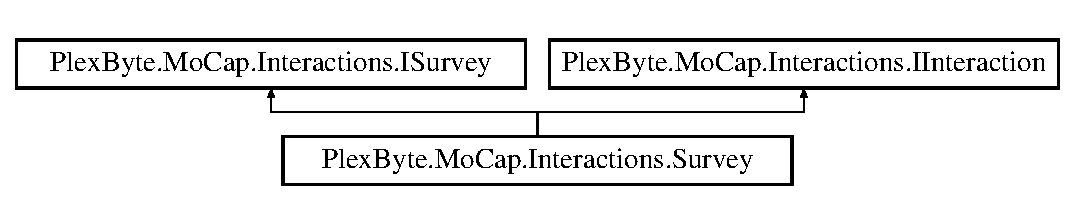
\includegraphics[height=2.000000cm]{class_plex_byte_1_1_mo_cap_1_1_interactions_1_1_survey}
\end{center}
\end{figure}
\subsection*{Public Member Functions}
\begin{DoxyCompactItemize}
\item 
\hyperlink{class_plex_byte_1_1_mo_cap_1_1_interactions_1_1_survey_a9ae20c258ed6e6ae23d242e329d4c06d}{Survey} (string p\+Id, string p\+Text, List$<$ \hyperlink{interface_plex_byte_1_1_mo_cap_1_1_interactions_1_1_i_survey_option}{I\+Survey\+Option} $>$ p\+Options, I\+User p\+Creator)
\begin{DoxyCompactList}\small\item\em Constructor of the class \end{DoxyCompactList}\item 
\hyperlink{class_plex_byte_1_1_mo_cap_1_1_interactions_1_1_survey_a76483d76195182900935fcd0d2382940}{Survey} (string p\+Id, string p\+Text, List$<$ string $>$ p\+Options, I\+User p\+Creator)
\begin{DoxyCompactList}\small\item\em Constructor of the class \end{DoxyCompactList}\item 
virtual void \hyperlink{class_plex_byte_1_1_mo_cap_1_1_interactions_1_1_survey_ae9f1ca5ffacd44917eda7458a335cefa}{On\+Complete} (\hyperlink{class_plex_byte_1_1_mo_cap_1_1_interactions_1_1_interaction_event_args}{Interaction\+Event\+Args} p\+Event\+Args)
\begin{DoxyCompactList}\small\item\em This method raises the corresponding event in case subscribers are registered \end{DoxyCompactList}\item 
virtual void \hyperlink{class_plex_byte_1_1_mo_cap_1_1_interactions_1_1_survey_a08208db03d7006c21d38e60fa7bd41f9}{On\+Modify} (\hyperlink{class_plex_byte_1_1_mo_cap_1_1_interactions_1_1_interaction_event_args}{Interaction\+Event\+Args} p\+Event\+Args)
\begin{DoxyCompactList}\small\item\em This method raises the corresponding event in case subscribers are registered \end{DoxyCompactList}\item 
virtual void \hyperlink{class_plex_byte_1_1_mo_cap_1_1_interactions_1_1_survey_a895f47ec3591749c04dbcfb329d8fae0}{On\+State\+Changed} (\hyperlink{class_plex_byte_1_1_mo_cap_1_1_interactions_1_1_interaction_event_args}{Interaction\+Event\+Args} p\+Event\+Args)
\begin{DoxyCompactList}\small\item\em This method raises the state\+Changed event, in case subscribers are registeres \end{DoxyCompactList}\item 
virtual void \hyperlink{class_plex_byte_1_1_mo_cap_1_1_interactions_1_1_survey_a1c301916ee78db1236c465cd3fe40449}{Change\+Owner} (I\+User p\+User)
\begin{DoxyCompactList}\small\item\em This method changes the owner of the survey and raises the modified event if the owner is different \end{DoxyCompactList}\item 
virtual void \hyperlink{class_plex_byte_1_1_mo_cap_1_1_interactions_1_1_survey_ab51b78828fafe0eaa305d6c80df91b0f}{Change\+Is\+Active} (bool p\+Active)
\begin{DoxyCompactList}\small\item\em This method changes the active flag of the object. This can occure if the item expired, finished or was cancelled. It will raise the Modified event once changed \end{DoxyCompactList}\item 
virtual void \hyperlink{class_plex_byte_1_1_mo_cap_1_1_interactions_1_1_survey_a0dcd8382de2ee659237dc0b25a388256}{Add\+Vote} (\hyperlink{interface_plex_byte_1_1_mo_cap_1_1_interactions_1_1_i_vote}{I\+Vote} p\+Vote)
\begin{DoxyCompactList}\small\item\em This method adds a vote to this survey and verifies if all votes were made. If this is the case a stat\+Changed event with state finished will be fired. It will also check if the user still has open votes \end{DoxyCompactList}\item 
virtual void \hyperlink{class_plex_byte_1_1_mo_cap_1_1_interactions_1_1_survey_a0a19d3bd2f79e716f256a76faeb850bc}{Add\+Option} (\hyperlink{interface_plex_byte_1_1_mo_cap_1_1_interactions_1_1_i_survey_option}{I\+Survey\+Option} p\+Option)
\begin{DoxyCompactList}\small\item\em This method will add options to a survey. In case a new option is added the Modified event is raised \end{DoxyCompactList}\item 
void \hyperlink{class_plex_byte_1_1_mo_cap_1_1_interactions_1_1_survey_a72758296f5dbc1e2f197705d51e1a827}{Add\+User} (I\+User p\+User)
\begin{DoxyCompactList}\small\item\em Adds a new user to the list of eligible users \end{DoxyCompactList}\item 
void \hyperlink{class_plex_byte_1_1_mo_cap_1_1_interactions_1_1_survey_ab274203ea62fab8cee7f9f32b29abba7}{Remove\+User} (I\+User p\+User)
\begin{DoxyCompactList}\small\item\em Removed a user from the list of eligible users \end{DoxyCompactList}\item 
void \hyperlink{class_plex_byte_1_1_mo_cap_1_1_interactions_1_1_survey_a7f44759a0d2ea7ce7516559fe8a70a94}{Change\+State} (\hyperlink{namespace_plex_byte_1_1_mo_cap_1_1_interactions_afcb673d9186608b6bd3b187179aedc8a}{Interaction\+State} p\+State)
\begin{DoxyCompactList}\small\item\em Changes the state of this interaction and thus causes the state\+C\+Hanged event to be fired \end{DoxyCompactList}\end{DoxyCompactItemize}
\subsection*{Public Attributes}
\begin{DoxyCompactItemize}
\item 
Date\+Time \hyperlink{class_plex_byte_1_1_mo_cap_1_1_interactions_1_1_survey_a408a891d3aceb61bb7a91e15084a7473}{Created\+Date\+Time} =$>$ \+\_\+created\+Date\+Time
\item 
bool \hyperlink{class_plex_byte_1_1_mo_cap_1_1_interactions_1_1_survey_aea8262119dda55b23d594cbadc4bb1d8}{Is\+Active} =$>$ \+\_\+is\+Active
\item 
I\+User \hyperlink{class_plex_byte_1_1_mo_cap_1_1_interactions_1_1_survey_af2a84b3a5f615138e34cda5b24f30cfd}{Creator} =$>$ \+\_\+creator
\item 
\hyperlink{namespace_plex_byte_1_1_mo_cap_1_1_interactions_afcb673d9186608b6bd3b187179aedc8a}{Interaction\+State} \hyperlink{class_plex_byte_1_1_mo_cap_1_1_interactions_1_1_survey_abd3fc51c6adfad7a540c70512303e280}{State} =$>$ \+\_\+state
\end{DoxyCompactItemize}
\subsection*{Properties}
\begin{DoxyCompactItemize}
\item 
List$<$ \hyperlink{interface_plex_byte_1_1_mo_cap_1_1_interactions_1_1_i_survey_option}{I\+Survey\+Option} $>$ \hyperlink{class_plex_byte_1_1_mo_cap_1_1_interactions_1_1_survey_adacfcf5546425c676756bd12772cb4e2}{Option\+List}\hspace{0.3cm}{\ttfamily  \mbox{[}get, set\mbox{]}}
\item 
List$<$ \hyperlink{interface_plex_byte_1_1_mo_cap_1_1_interactions_1_1_i_vote}{I\+Vote} $>$ \hyperlink{class_plex_byte_1_1_mo_cap_1_1_interactions_1_1_survey_a3527ea8b21abf85da934d6940a97d2ea}{Vote\+List}\hspace{0.3cm}{\ttfamily  \mbox{[}get, set\mbox{]}}
\item 
string \hyperlink{class_plex_byte_1_1_mo_cap_1_1_interactions_1_1_survey_a590e6dd00026c7c039fd61e3166b7170}{Title}\hspace{0.3cm}{\ttfamily  \mbox{[}get, set\mbox{]}}
\item 
string \hyperlink{class_plex_byte_1_1_mo_cap_1_1_interactions_1_1_survey_a8d9364d1707414404e0056c269c37697}{Interaction\+Id}\hspace{0.3cm}{\ttfamily  \mbox{[}get, set\mbox{]}}
\item 
string \hyperlink{class_plex_byte_1_1_mo_cap_1_1_interactions_1_1_survey_afebba71a8a4961e1cc28c18ad42b7c98}{Project\+Id}\hspace{0.3cm}{\ttfamily  \mbox{[}get, set\mbox{]}}
\item 
Date\+Time \hyperlink{class_plex_byte_1_1_mo_cap_1_1_interactions_1_1_survey_a890e2c1421c46175b9fb9af925b57ecf}{Start\+Date\+Time}\hspace{0.3cm}{\ttfamily  \mbox{[}get, set\mbox{]}}
\item 
Date\+Time \hyperlink{class_plex_byte_1_1_mo_cap_1_1_interactions_1_1_survey_ad848704707f53e6e58a081dea98c4072}{End\+Date\+Time}\hspace{0.3cm}{\ttfamily  \mbox{[}get, set\mbox{]}}
\item 
Date\+Time \hyperlink{class_plex_byte_1_1_mo_cap_1_1_interactions_1_1_survey_adcfad739d1a4acf70ed60a035716f1d1}{Modified\+Date\+Time}\hspace{0.3cm}{\ttfamily  \mbox{[}get, set\mbox{]}}
\item 
string \hyperlink{class_plex_byte_1_1_mo_cap_1_1_interactions_1_1_survey_ade12b9b3a140efb18dd061665b40224d}{Text}\hspace{0.3cm}{\ttfamily  \mbox{[}get, set\mbox{]}}
\item 
\hyperlink{namespace_plex_byte_1_1_mo_cap_1_1_interactions_a6e7bea333446664bbce2bb296db25e31}{Interaction\+Type} \hyperlink{class_plex_byte_1_1_mo_cap_1_1_interactions_1_1_survey_a339b8292ba9abcab9a2f1aad096bb264}{Type}\hspace{0.3cm}{\ttfamily  \mbox{[}get, set\mbox{]}}
\item 
I\+User \hyperlink{class_plex_byte_1_1_mo_cap_1_1_interactions_1_1_survey_ae4f5e62e3d0f98f34551ec82003ff2ee}{Owner}\hspace{0.3cm}{\ttfamily  \mbox{[}get, set\mbox{]}}
\item 
Date\+Time \hyperlink{class_plex_byte_1_1_mo_cap_1_1_interactions_1_1_survey_a593beaaf80e5c08e1747bf9664258799}{Due\+Date\+Time}\hspace{0.3cm}{\ttfamily  \mbox{[}get, set\mbox{]}}
\item 
int \hyperlink{class_plex_byte_1_1_mo_cap_1_1_interactions_1_1_survey_ad7edb8b491c86a65a4a604388e730b9c}{Max\+Votes\+Per\+User}\hspace{0.3cm}{\ttfamily  \mbox{[}get, set\mbox{]}}
\item 
List$<$ I\+User $>$ \hyperlink{class_plex_byte_1_1_mo_cap_1_1_interactions_1_1_survey_abf34631f6e58537dbdfef1914ff863f9}{User\+List}\hspace{0.3cm}{\ttfamily  \mbox{[}get, set\mbox{]}}
\item 
string \hyperlink{class_plex_byte_1_1_mo_cap_1_1_interactions_1_1_survey_a7d24bb1bc8db75b6f2b8751cdf7e83f1}{Id}\hspace{0.3cm}{\ttfamily  \mbox{[}get, set\mbox{]}}
\end{DoxyCompactItemize}
\subsection*{Events}
\begin{DoxyCompactItemize}
\item 
\hyperlink{namespace_plex_byte_1_1_mo_cap_1_1_interactions_ac81ac3321ab2b018c75ad2c18ec15b9e}{Complete} \hyperlink{class_plex_byte_1_1_mo_cap_1_1_interactions_1_1_survey_a954056f9deb35fc271a4c8932003b832}{Completed}
\item 
\hyperlink{namespace_plex_byte_1_1_mo_cap_1_1_interactions_a490186f613e46adce26244f3b2c78a58}{Modify} \hyperlink{class_plex_byte_1_1_mo_cap_1_1_interactions_1_1_survey_a92a7ef7437f99640fea44765d7453418}{Modified}
\item 
\hyperlink{namespace_plex_byte_1_1_mo_cap_1_1_interactions_af2ff213e81451f96fc74bfad114cecde}{State\+Change} \hyperlink{class_plex_byte_1_1_mo_cap_1_1_interactions_1_1_survey_afaec6df3811245396b6f4bfc3062a0c9}{State\+Changed}
\end{DoxyCompactItemize}


\subsection{Detailed Description}


Definition at line 11 of file Survey.\+cs.



\subsection{Constructor \& Destructor Documentation}
\index{Plex\+Byte\+::\+Mo\+Cap\+::\+Interactions\+::\+Survey@{Plex\+Byte\+::\+Mo\+Cap\+::\+Interactions\+::\+Survey}!Survey@{Survey}}
\index{Survey@{Survey}!Plex\+Byte\+::\+Mo\+Cap\+::\+Interactions\+::\+Survey@{Plex\+Byte\+::\+Mo\+Cap\+::\+Interactions\+::\+Survey}}
\subsubsection[{\texorpdfstring{Survey(string p\+Id, string p\+Text, List$<$ I\+Survey\+Option $>$ p\+Options, I\+User p\+Creator)}{Survey(string pId, string pText, List< ISurveyOption > pOptions, IUser pCreator)}}]{\setlength{\rightskip}{0pt plus 5cm}Plex\+Byte.\+Mo\+Cap.\+Interactions.\+Survey.\+Survey (
\begin{DoxyParamCaption}
\item[{string}]{p\+Id, }
\item[{string}]{p\+Text, }
\item[{List$<$ {\bf I\+Survey\+Option} $>$}]{p\+Options, }
\item[{I\+User}]{p\+Creator}
\end{DoxyParamCaption}
)}\hypertarget{class_plex_byte_1_1_mo_cap_1_1_interactions_1_1_survey_a9ae20c258ed6e6ae23d242e329d4c06d}{}\label{class_plex_byte_1_1_mo_cap_1_1_interactions_1_1_survey_a9ae20c258ed6e6ae23d242e329d4c06d}


Constructor of the class 


\begin{DoxyParams}{Parameters}
{\em p\+Id} & The id of the interaction\\
\hline
{\em p\+Text} & The text of the survey\\
\hline
{\em p\+Options} & The options available\\
\hline
{\em p\+Creator} & The creator of this survey\\
\hline
\end{DoxyParams}


Definition at line 66 of file Survey.\+cs.

\index{Plex\+Byte\+::\+Mo\+Cap\+::\+Interactions\+::\+Survey@{Plex\+Byte\+::\+Mo\+Cap\+::\+Interactions\+::\+Survey}!Survey@{Survey}}
\index{Survey@{Survey}!Plex\+Byte\+::\+Mo\+Cap\+::\+Interactions\+::\+Survey@{Plex\+Byte\+::\+Mo\+Cap\+::\+Interactions\+::\+Survey}}
\subsubsection[{\texorpdfstring{Survey(string p\+Id, string p\+Text, List$<$ string $>$ p\+Options, I\+User p\+Creator)}{Survey(string pId, string pText, List< string > pOptions, IUser pCreator)}}]{\setlength{\rightskip}{0pt plus 5cm}Plex\+Byte.\+Mo\+Cap.\+Interactions.\+Survey.\+Survey (
\begin{DoxyParamCaption}
\item[{string}]{p\+Id, }
\item[{string}]{p\+Text, }
\item[{List$<$ string $>$}]{p\+Options, }
\item[{I\+User}]{p\+Creator}
\end{DoxyParamCaption}
)}\hypertarget{class_plex_byte_1_1_mo_cap_1_1_interactions_1_1_survey_a76483d76195182900935fcd0d2382940}{}\label{class_plex_byte_1_1_mo_cap_1_1_interactions_1_1_survey_a76483d76195182900935fcd0d2382940}


Constructor of the class 


\begin{DoxyParams}{Parameters}
{\em p\+Id} & The id of the interaction\\
\hline
{\em p\+Text} & The text of the survey\\
\hline
{\em p\+Options} & The options available as strngs\\
\hline
{\em p\+Creator} & The creator of this survey\\
\hline
\end{DoxyParams}


Definition at line 75 of file Survey.\+cs.



\subsection{Member Function Documentation}
\index{Plex\+Byte\+::\+Mo\+Cap\+::\+Interactions\+::\+Survey@{Plex\+Byte\+::\+Mo\+Cap\+::\+Interactions\+::\+Survey}!Add\+Option@{Add\+Option}}
\index{Add\+Option@{Add\+Option}!Plex\+Byte\+::\+Mo\+Cap\+::\+Interactions\+::\+Survey@{Plex\+Byte\+::\+Mo\+Cap\+::\+Interactions\+::\+Survey}}
\subsubsection[{\texorpdfstring{Add\+Option(\+I\+Survey\+Option p\+Option)}{AddOption(ISurveyOption pOption)}}]{\setlength{\rightskip}{0pt plus 5cm}virtual void Plex\+Byte.\+Mo\+Cap.\+Interactions.\+Survey.\+Add\+Option (
\begin{DoxyParamCaption}
\item[{{\bf I\+Survey\+Option}}]{p\+Option}
\end{DoxyParamCaption}
)\hspace{0.3cm}{\ttfamily [virtual]}}\hypertarget{class_plex_byte_1_1_mo_cap_1_1_interactions_1_1_survey_a0a19d3bd2f79e716f256a76faeb850bc}{}\label{class_plex_byte_1_1_mo_cap_1_1_interactions_1_1_survey_a0a19d3bd2f79e716f256a76faeb850bc}


This method will add options to a survey. In case a new option is added the Modified event is raised 


\begin{DoxyParams}{Parameters}
{\em p\+Option} & The survey option to add\\
\hline
\end{DoxyParams}


Implements \hyperlink{interface_plex_byte_1_1_mo_cap_1_1_interactions_1_1_i_survey_a19e6f79d6fc9ba6c8947894a0ab0d811}{Plex\+Byte.\+Mo\+Cap.\+Interactions.\+I\+Survey}.



Definition at line 166 of file Survey.\+cs.

\index{Plex\+Byte\+::\+Mo\+Cap\+::\+Interactions\+::\+Survey@{Plex\+Byte\+::\+Mo\+Cap\+::\+Interactions\+::\+Survey}!Add\+User@{Add\+User}}
\index{Add\+User@{Add\+User}!Plex\+Byte\+::\+Mo\+Cap\+::\+Interactions\+::\+Survey@{Plex\+Byte\+::\+Mo\+Cap\+::\+Interactions\+::\+Survey}}
\subsubsection[{\texorpdfstring{Add\+User(\+I\+User p\+User)}{AddUser(IUser pUser)}}]{\setlength{\rightskip}{0pt plus 5cm}void Plex\+Byte.\+Mo\+Cap.\+Interactions.\+Survey.\+Add\+User (
\begin{DoxyParamCaption}
\item[{I\+User}]{p\+User}
\end{DoxyParamCaption}
)}\hypertarget{class_plex_byte_1_1_mo_cap_1_1_interactions_1_1_survey_a72758296f5dbc1e2f197705d51e1a827}{}\label{class_plex_byte_1_1_mo_cap_1_1_interactions_1_1_survey_a72758296f5dbc1e2f197705d51e1a827}


Adds a new user to the list of eligible users 


\begin{DoxyParams}{Parameters}
{\em p\+User} & The user to add\\
\hline
\end{DoxyParams}


Implements \hyperlink{interface_plex_byte_1_1_mo_cap_1_1_interactions_1_1_i_survey_a252050839e9167b57648e150a65385ea}{Plex\+Byte.\+Mo\+Cap.\+Interactions.\+I\+Survey}.



Definition at line 180 of file Survey.\+cs.

\index{Plex\+Byte\+::\+Mo\+Cap\+::\+Interactions\+::\+Survey@{Plex\+Byte\+::\+Mo\+Cap\+::\+Interactions\+::\+Survey}!Add\+Vote@{Add\+Vote}}
\index{Add\+Vote@{Add\+Vote}!Plex\+Byte\+::\+Mo\+Cap\+::\+Interactions\+::\+Survey@{Plex\+Byte\+::\+Mo\+Cap\+::\+Interactions\+::\+Survey}}
\subsubsection[{\texorpdfstring{Add\+Vote(\+I\+Vote p\+Vote)}{AddVote(IVote pVote)}}]{\setlength{\rightskip}{0pt plus 5cm}virtual void Plex\+Byte.\+Mo\+Cap.\+Interactions.\+Survey.\+Add\+Vote (
\begin{DoxyParamCaption}
\item[{{\bf I\+Vote}}]{p\+Vote}
\end{DoxyParamCaption}
)\hspace{0.3cm}{\ttfamily [virtual]}}\hypertarget{class_plex_byte_1_1_mo_cap_1_1_interactions_1_1_survey_a0dcd8382de2ee659237dc0b25a388256}{}\label{class_plex_byte_1_1_mo_cap_1_1_interactions_1_1_survey_a0dcd8382de2ee659237dc0b25a388256}


This method adds a vote to this survey and verifies if all votes were made. If this is the case a stat\+Changed event with state finished will be fired. It will also check if the user still has open votes 


\begin{DoxyParams}{Parameters}
{\em p\+Vote} & The vote to ass\\
\hline
\end{DoxyParams}


Implements \hyperlink{interface_plex_byte_1_1_mo_cap_1_1_interactions_1_1_i_survey_ab9df3eb58a1c66b14412cd1bd26f038c}{Plex\+Byte.\+Mo\+Cap.\+Interactions.\+I\+Survey}.



Definition at line 145 of file Survey.\+cs.

\index{Plex\+Byte\+::\+Mo\+Cap\+::\+Interactions\+::\+Survey@{Plex\+Byte\+::\+Mo\+Cap\+::\+Interactions\+::\+Survey}!Change\+Is\+Active@{Change\+Is\+Active}}
\index{Change\+Is\+Active@{Change\+Is\+Active}!Plex\+Byte\+::\+Mo\+Cap\+::\+Interactions\+::\+Survey@{Plex\+Byte\+::\+Mo\+Cap\+::\+Interactions\+::\+Survey}}
\subsubsection[{\texorpdfstring{Change\+Is\+Active(bool p\+Active)}{ChangeIsActive(bool pActive)}}]{\setlength{\rightskip}{0pt plus 5cm}virtual void Plex\+Byte.\+Mo\+Cap.\+Interactions.\+Survey.\+Change\+Is\+Active (
\begin{DoxyParamCaption}
\item[{bool}]{p\+Active}
\end{DoxyParamCaption}
)\hspace{0.3cm}{\ttfamily [virtual]}}\hypertarget{class_plex_byte_1_1_mo_cap_1_1_interactions_1_1_survey_ab51b78828fafe0eaa305d6c80df91b0f}{}\label{class_plex_byte_1_1_mo_cap_1_1_interactions_1_1_survey_ab51b78828fafe0eaa305d6c80df91b0f}


This method changes the active flag of the object. This can occure if the item expired, finished or was cancelled. It will raise the Modified event once changed 


\begin{DoxyParams}{Parameters}
{\em p\+Active} & \\
\hline
\end{DoxyParams}


Implements \hyperlink{interface_plex_byte_1_1_mo_cap_1_1_interactions_1_1_i_interaction_ac2d9f47a1139b931939e8cff07153aba}{Plex\+Byte.\+Mo\+Cap.\+Interactions.\+I\+Interaction}.



Definition at line 130 of file Survey.\+cs.

\index{Plex\+Byte\+::\+Mo\+Cap\+::\+Interactions\+::\+Survey@{Plex\+Byte\+::\+Mo\+Cap\+::\+Interactions\+::\+Survey}!Change\+Owner@{Change\+Owner}}
\index{Change\+Owner@{Change\+Owner}!Plex\+Byte\+::\+Mo\+Cap\+::\+Interactions\+::\+Survey@{Plex\+Byte\+::\+Mo\+Cap\+::\+Interactions\+::\+Survey}}
\subsubsection[{\texorpdfstring{Change\+Owner(\+I\+User p\+User)}{ChangeOwner(IUser pUser)}}]{\setlength{\rightskip}{0pt plus 5cm}virtual void Plex\+Byte.\+Mo\+Cap.\+Interactions.\+Survey.\+Change\+Owner (
\begin{DoxyParamCaption}
\item[{I\+User}]{p\+User}
\end{DoxyParamCaption}
)\hspace{0.3cm}{\ttfamily [virtual]}}\hypertarget{class_plex_byte_1_1_mo_cap_1_1_interactions_1_1_survey_a1c301916ee78db1236c465cd3fe40449}{}\label{class_plex_byte_1_1_mo_cap_1_1_interactions_1_1_survey_a1c301916ee78db1236c465cd3fe40449}


This method changes the owner of the survey and raises the modified event if the owner is different 


\begin{DoxyParams}{Parameters}
{\em p\+User} & The new user to mark as owner\\
\hline
\end{DoxyParams}


Implements \hyperlink{interface_plex_byte_1_1_mo_cap_1_1_interactions_1_1_i_interaction_a7e3b0a67dc7d176877b8b94922a9bb52}{Plex\+Byte.\+Mo\+Cap.\+Interactions.\+I\+Interaction}.



Definition at line 115 of file Survey.\+cs.

\index{Plex\+Byte\+::\+Mo\+Cap\+::\+Interactions\+::\+Survey@{Plex\+Byte\+::\+Mo\+Cap\+::\+Interactions\+::\+Survey}!Change\+State@{Change\+State}}
\index{Change\+State@{Change\+State}!Plex\+Byte\+::\+Mo\+Cap\+::\+Interactions\+::\+Survey@{Plex\+Byte\+::\+Mo\+Cap\+::\+Interactions\+::\+Survey}}
\subsubsection[{\texorpdfstring{Change\+State(\+Interaction\+State p\+State)}{ChangeState(InteractionState pState)}}]{\setlength{\rightskip}{0pt plus 5cm}void Plex\+Byte.\+Mo\+Cap.\+Interactions.\+Survey.\+Change\+State (
\begin{DoxyParamCaption}
\item[{{\bf Interaction\+State}}]{p\+State}
\end{DoxyParamCaption}
)}\hypertarget{class_plex_byte_1_1_mo_cap_1_1_interactions_1_1_survey_a7f44759a0d2ea7ce7516559fe8a70a94}{}\label{class_plex_byte_1_1_mo_cap_1_1_interactions_1_1_survey_a7f44759a0d2ea7ce7516559fe8a70a94}


Changes the state of this interaction and thus causes the state\+C\+Hanged event to be fired 


\begin{DoxyParams}{Parameters}
{\em p\+State} & The new state to set\\
\hline
\end{DoxyParams}


Implements \hyperlink{interface_plex_byte_1_1_mo_cap_1_1_interactions_1_1_i_interaction_a10beb35eb6061878469b5a6cd5431b32}{Plex\+Byte.\+Mo\+Cap.\+Interactions.\+I\+Interaction}.



Definition at line 208 of file Survey.\+cs.

\index{Plex\+Byte\+::\+Mo\+Cap\+::\+Interactions\+::\+Survey@{Plex\+Byte\+::\+Mo\+Cap\+::\+Interactions\+::\+Survey}!On\+Complete@{On\+Complete}}
\index{On\+Complete@{On\+Complete}!Plex\+Byte\+::\+Mo\+Cap\+::\+Interactions\+::\+Survey@{Plex\+Byte\+::\+Mo\+Cap\+::\+Interactions\+::\+Survey}}
\subsubsection[{\texorpdfstring{On\+Complete(\+Interaction\+Event\+Args p\+Event\+Args)}{OnComplete(InteractionEventArgs pEventArgs)}}]{\setlength{\rightskip}{0pt plus 5cm}virtual void Plex\+Byte.\+Mo\+Cap.\+Interactions.\+Survey.\+On\+Complete (
\begin{DoxyParamCaption}
\item[{{\bf Interaction\+Event\+Args}}]{p\+Event\+Args}
\end{DoxyParamCaption}
)\hspace{0.3cm}{\ttfamily [virtual]}}\hypertarget{class_plex_byte_1_1_mo_cap_1_1_interactions_1_1_survey_ae9f1ca5ffacd44917eda7458a335cefa}{}\label{class_plex_byte_1_1_mo_cap_1_1_interactions_1_1_survey_ae9f1ca5ffacd44917eda7458a335cefa}


This method raises the corresponding event in case subscribers are registered 


\begin{DoxyParams}{Parameters}
{\em p\+Event\+Args} & The event args to pass along\\
\hline
\end{DoxyParams}


Implements \hyperlink{interface_plex_byte_1_1_mo_cap_1_1_interactions_1_1_i_interaction_a9f32d6c1c2f2ae60dabb274f62128447}{Plex\+Byte.\+Mo\+Cap.\+Interactions.\+I\+Interaction}.



Definition at line 93 of file Survey.\+cs.

\index{Plex\+Byte\+::\+Mo\+Cap\+::\+Interactions\+::\+Survey@{Plex\+Byte\+::\+Mo\+Cap\+::\+Interactions\+::\+Survey}!On\+Modify@{On\+Modify}}
\index{On\+Modify@{On\+Modify}!Plex\+Byte\+::\+Mo\+Cap\+::\+Interactions\+::\+Survey@{Plex\+Byte\+::\+Mo\+Cap\+::\+Interactions\+::\+Survey}}
\subsubsection[{\texorpdfstring{On\+Modify(\+Interaction\+Event\+Args p\+Event\+Args)}{OnModify(InteractionEventArgs pEventArgs)}}]{\setlength{\rightskip}{0pt plus 5cm}virtual void Plex\+Byte.\+Mo\+Cap.\+Interactions.\+Survey.\+On\+Modify (
\begin{DoxyParamCaption}
\item[{{\bf Interaction\+Event\+Args}}]{p\+Event\+Args}
\end{DoxyParamCaption}
)\hspace{0.3cm}{\ttfamily [virtual]}}\hypertarget{class_plex_byte_1_1_mo_cap_1_1_interactions_1_1_survey_a08208db03d7006c21d38e60fa7bd41f9}{}\label{class_plex_byte_1_1_mo_cap_1_1_interactions_1_1_survey_a08208db03d7006c21d38e60fa7bd41f9}


This method raises the corresponding event in case subscribers are registered 


\begin{DoxyParams}{Parameters}
{\em p\+Event\+Args} & The event args to pass along\\
\hline
\end{DoxyParams}


Implements \hyperlink{interface_plex_byte_1_1_mo_cap_1_1_interactions_1_1_i_interaction_af4fac42d753ae7f9652541542b8961c6}{Plex\+Byte.\+Mo\+Cap.\+Interactions.\+I\+Interaction}.



Definition at line 99 of file Survey.\+cs.

\index{Plex\+Byte\+::\+Mo\+Cap\+::\+Interactions\+::\+Survey@{Plex\+Byte\+::\+Mo\+Cap\+::\+Interactions\+::\+Survey}!On\+State\+Changed@{On\+State\+Changed}}
\index{On\+State\+Changed@{On\+State\+Changed}!Plex\+Byte\+::\+Mo\+Cap\+::\+Interactions\+::\+Survey@{Plex\+Byte\+::\+Mo\+Cap\+::\+Interactions\+::\+Survey}}
\subsubsection[{\texorpdfstring{On\+State\+Changed(\+Interaction\+Event\+Args p\+Event\+Args)}{OnStateChanged(InteractionEventArgs pEventArgs)}}]{\setlength{\rightskip}{0pt plus 5cm}virtual void Plex\+Byte.\+Mo\+Cap.\+Interactions.\+Survey.\+On\+State\+Changed (
\begin{DoxyParamCaption}
\item[{{\bf Interaction\+Event\+Args}}]{p\+Event\+Args}
\end{DoxyParamCaption}
)\hspace{0.3cm}{\ttfamily [virtual]}}\hypertarget{class_plex_byte_1_1_mo_cap_1_1_interactions_1_1_survey_a895f47ec3591749c04dbcfb329d8fae0}{}\label{class_plex_byte_1_1_mo_cap_1_1_interactions_1_1_survey_a895f47ec3591749c04dbcfb329d8fae0}


This method raises the state\+Changed event, in case subscribers are registeres 


\begin{DoxyParams}{Parameters}
{\em p\+Event\+Args} & The event args to pass along\\
\hline
\end{DoxyParams}


Implements \hyperlink{interface_plex_byte_1_1_mo_cap_1_1_interactions_1_1_i_interaction_a5250247fb5f22a633e22d7f8dc946c4d}{Plex\+Byte.\+Mo\+Cap.\+Interactions.\+I\+Interaction}.



Definition at line 105 of file Survey.\+cs.

\index{Plex\+Byte\+::\+Mo\+Cap\+::\+Interactions\+::\+Survey@{Plex\+Byte\+::\+Mo\+Cap\+::\+Interactions\+::\+Survey}!Remove\+User@{Remove\+User}}
\index{Remove\+User@{Remove\+User}!Plex\+Byte\+::\+Mo\+Cap\+::\+Interactions\+::\+Survey@{Plex\+Byte\+::\+Mo\+Cap\+::\+Interactions\+::\+Survey}}
\subsubsection[{\texorpdfstring{Remove\+User(\+I\+User p\+User)}{RemoveUser(IUser pUser)}}]{\setlength{\rightskip}{0pt plus 5cm}void Plex\+Byte.\+Mo\+Cap.\+Interactions.\+Survey.\+Remove\+User (
\begin{DoxyParamCaption}
\item[{I\+User}]{p\+User}
\end{DoxyParamCaption}
)}\hypertarget{class_plex_byte_1_1_mo_cap_1_1_interactions_1_1_survey_ab274203ea62fab8cee7f9f32b29abba7}{}\label{class_plex_byte_1_1_mo_cap_1_1_interactions_1_1_survey_ab274203ea62fab8cee7f9f32b29abba7}


Removed a user from the list of eligible users 


\begin{DoxyParams}{Parameters}
{\em p\+User} & The user to remove\\
\hline
\end{DoxyParams}


Implements \hyperlink{interface_plex_byte_1_1_mo_cap_1_1_interactions_1_1_i_survey_a0e4b923ee86fb5031f0eaa9e3c81dbbd}{Plex\+Byte.\+Mo\+Cap.\+Interactions.\+I\+Survey}.



Definition at line 194 of file Survey.\+cs.



\subsection{Member Data Documentation}
\index{Plex\+Byte\+::\+Mo\+Cap\+::\+Interactions\+::\+Survey@{Plex\+Byte\+::\+Mo\+Cap\+::\+Interactions\+::\+Survey}!Created\+Date\+Time@{Created\+Date\+Time}}
\index{Created\+Date\+Time@{Created\+Date\+Time}!Plex\+Byte\+::\+Mo\+Cap\+::\+Interactions\+::\+Survey@{Plex\+Byte\+::\+Mo\+Cap\+::\+Interactions\+::\+Survey}}
\subsubsection[{\texorpdfstring{Created\+Date\+Time}{CreatedDateTime}}]{\setlength{\rightskip}{0pt plus 5cm}Date\+Time Plex\+Byte.\+Mo\+Cap.\+Interactions.\+Survey.\+Created\+Date\+Time =$>$ \+\_\+created\+Date\+Time}\hypertarget{class_plex_byte_1_1_mo_cap_1_1_interactions_1_1_survey_a408a891d3aceb61bb7a91e15084a7473}{}\label{class_plex_byte_1_1_mo_cap_1_1_interactions_1_1_survey_a408a891d3aceb61bb7a91e15084a7473}


Definition at line 23 of file Survey.\+cs.

\index{Plex\+Byte\+::\+Mo\+Cap\+::\+Interactions\+::\+Survey@{Plex\+Byte\+::\+Mo\+Cap\+::\+Interactions\+::\+Survey}!Creator@{Creator}}
\index{Creator@{Creator}!Plex\+Byte\+::\+Mo\+Cap\+::\+Interactions\+::\+Survey@{Plex\+Byte\+::\+Mo\+Cap\+::\+Interactions\+::\+Survey}}
\subsubsection[{\texorpdfstring{Creator}{Creator}}]{\setlength{\rightskip}{0pt plus 5cm}I\+User Plex\+Byte.\+Mo\+Cap.\+Interactions.\+Survey.\+Creator =$>$ \+\_\+creator}\hypertarget{class_plex_byte_1_1_mo_cap_1_1_interactions_1_1_survey_af2a84b3a5f615138e34cda5b24f30cfd}{}\label{class_plex_byte_1_1_mo_cap_1_1_interactions_1_1_survey_af2a84b3a5f615138e34cda5b24f30cfd}


Definition at line 28 of file Survey.\+cs.

\index{Plex\+Byte\+::\+Mo\+Cap\+::\+Interactions\+::\+Survey@{Plex\+Byte\+::\+Mo\+Cap\+::\+Interactions\+::\+Survey}!Is\+Active@{Is\+Active}}
\index{Is\+Active@{Is\+Active}!Plex\+Byte\+::\+Mo\+Cap\+::\+Interactions\+::\+Survey@{Plex\+Byte\+::\+Mo\+Cap\+::\+Interactions\+::\+Survey}}
\subsubsection[{\texorpdfstring{Is\+Active}{IsActive}}]{\setlength{\rightskip}{0pt plus 5cm}bool Plex\+Byte.\+Mo\+Cap.\+Interactions.\+Survey.\+Is\+Active =$>$ \+\_\+is\+Active}\hypertarget{class_plex_byte_1_1_mo_cap_1_1_interactions_1_1_survey_aea8262119dda55b23d594cbadc4bb1d8}{}\label{class_plex_byte_1_1_mo_cap_1_1_interactions_1_1_survey_aea8262119dda55b23d594cbadc4bb1d8}


Definition at line 25 of file Survey.\+cs.

\index{Plex\+Byte\+::\+Mo\+Cap\+::\+Interactions\+::\+Survey@{Plex\+Byte\+::\+Mo\+Cap\+::\+Interactions\+::\+Survey}!State@{State}}
\index{State@{State}!Plex\+Byte\+::\+Mo\+Cap\+::\+Interactions\+::\+Survey@{Plex\+Byte\+::\+Mo\+Cap\+::\+Interactions\+::\+Survey}}
\subsubsection[{\texorpdfstring{State}{State}}]{\setlength{\rightskip}{0pt plus 5cm}{\bf Interaction\+State} Plex\+Byte.\+Mo\+Cap.\+Interactions.\+Survey.\+State =$>$ \+\_\+state}\hypertarget{class_plex_byte_1_1_mo_cap_1_1_interactions_1_1_survey_abd3fc51c6adfad7a540c70512303e280}{}\label{class_plex_byte_1_1_mo_cap_1_1_interactions_1_1_survey_abd3fc51c6adfad7a540c70512303e280}


Definition at line 31 of file Survey.\+cs.



\subsection{Property Documentation}
\index{Plex\+Byte\+::\+Mo\+Cap\+::\+Interactions\+::\+Survey@{Plex\+Byte\+::\+Mo\+Cap\+::\+Interactions\+::\+Survey}!Due\+Date\+Time@{Due\+Date\+Time}}
\index{Due\+Date\+Time@{Due\+Date\+Time}!Plex\+Byte\+::\+Mo\+Cap\+::\+Interactions\+::\+Survey@{Plex\+Byte\+::\+Mo\+Cap\+::\+Interactions\+::\+Survey}}
\subsubsection[{\texorpdfstring{Due\+Date\+Time}{DueDateTime}}]{\setlength{\rightskip}{0pt plus 5cm}Date\+Time Plex\+Byte.\+Mo\+Cap.\+Interactions.\+Survey.\+Due\+Date\+Time\hspace{0.3cm}{\ttfamily [get]}, {\ttfamily [set]}}\hypertarget{class_plex_byte_1_1_mo_cap_1_1_interactions_1_1_survey_a593beaaf80e5c08e1747bf9664258799}{}\label{class_plex_byte_1_1_mo_cap_1_1_interactions_1_1_survey_a593beaaf80e5c08e1747bf9664258799}


Definition at line 30 of file Survey.\+cs.

\index{Plex\+Byte\+::\+Mo\+Cap\+::\+Interactions\+::\+Survey@{Plex\+Byte\+::\+Mo\+Cap\+::\+Interactions\+::\+Survey}!End\+Date\+Time@{End\+Date\+Time}}
\index{End\+Date\+Time@{End\+Date\+Time}!Plex\+Byte\+::\+Mo\+Cap\+::\+Interactions\+::\+Survey@{Plex\+Byte\+::\+Mo\+Cap\+::\+Interactions\+::\+Survey}}
\subsubsection[{\texorpdfstring{End\+Date\+Time}{EndDateTime}}]{\setlength{\rightskip}{0pt plus 5cm}Date\+Time Plex\+Byte.\+Mo\+Cap.\+Interactions.\+Survey.\+End\+Date\+Time\hspace{0.3cm}{\ttfamily [get]}, {\ttfamily [set]}}\hypertarget{class_plex_byte_1_1_mo_cap_1_1_interactions_1_1_survey_ad848704707f53e6e58a081dea98c4072}{}\label{class_plex_byte_1_1_mo_cap_1_1_interactions_1_1_survey_ad848704707f53e6e58a081dea98c4072}


Definition at line 22 of file Survey.\+cs.

\index{Plex\+Byte\+::\+Mo\+Cap\+::\+Interactions\+::\+Survey@{Plex\+Byte\+::\+Mo\+Cap\+::\+Interactions\+::\+Survey}!Id@{Id}}
\index{Id@{Id}!Plex\+Byte\+::\+Mo\+Cap\+::\+Interactions\+::\+Survey@{Plex\+Byte\+::\+Mo\+Cap\+::\+Interactions\+::\+Survey}}
\subsubsection[{\texorpdfstring{Id}{Id}}]{\setlength{\rightskip}{0pt plus 5cm}string Plex\+Byte.\+Mo\+Cap.\+Interactions.\+Survey.\+Id\hspace{0.3cm}{\ttfamily [get]}, {\ttfamily [set]}}\hypertarget{class_plex_byte_1_1_mo_cap_1_1_interactions_1_1_survey_a7d24bb1bc8db75b6f2b8751cdf7e83f1}{}\label{class_plex_byte_1_1_mo_cap_1_1_interactions_1_1_survey_a7d24bb1bc8db75b6f2b8751cdf7e83f1}


Definition at line 35 of file Survey.\+cs.

\index{Plex\+Byte\+::\+Mo\+Cap\+::\+Interactions\+::\+Survey@{Plex\+Byte\+::\+Mo\+Cap\+::\+Interactions\+::\+Survey}!Interaction\+Id@{Interaction\+Id}}
\index{Interaction\+Id@{Interaction\+Id}!Plex\+Byte\+::\+Mo\+Cap\+::\+Interactions\+::\+Survey@{Plex\+Byte\+::\+Mo\+Cap\+::\+Interactions\+::\+Survey}}
\subsubsection[{\texorpdfstring{Interaction\+Id}{InteractionId}}]{\setlength{\rightskip}{0pt plus 5cm}string Plex\+Byte.\+Mo\+Cap.\+Interactions.\+Survey.\+Interaction\+Id\hspace{0.3cm}{\ttfamily [get]}, {\ttfamily [set]}}\hypertarget{class_plex_byte_1_1_mo_cap_1_1_interactions_1_1_survey_a8d9364d1707414404e0056c269c37697}{}\label{class_plex_byte_1_1_mo_cap_1_1_interactions_1_1_survey_a8d9364d1707414404e0056c269c37697}


Definition at line 19 of file Survey.\+cs.

\index{Plex\+Byte\+::\+Mo\+Cap\+::\+Interactions\+::\+Survey@{Plex\+Byte\+::\+Mo\+Cap\+::\+Interactions\+::\+Survey}!Max\+Votes\+Per\+User@{Max\+Votes\+Per\+User}}
\index{Max\+Votes\+Per\+User@{Max\+Votes\+Per\+User}!Plex\+Byte\+::\+Mo\+Cap\+::\+Interactions\+::\+Survey@{Plex\+Byte\+::\+Mo\+Cap\+::\+Interactions\+::\+Survey}}
\subsubsection[{\texorpdfstring{Max\+Votes\+Per\+User}{MaxVotesPerUser}}]{\setlength{\rightskip}{0pt plus 5cm}int Plex\+Byte.\+Mo\+Cap.\+Interactions.\+Survey.\+Max\+Votes\+Per\+User\hspace{0.3cm}{\ttfamily [get]}, {\ttfamily [set]}}\hypertarget{class_plex_byte_1_1_mo_cap_1_1_interactions_1_1_survey_ad7edb8b491c86a65a4a604388e730b9c}{}\label{class_plex_byte_1_1_mo_cap_1_1_interactions_1_1_survey_ad7edb8b491c86a65a4a604388e730b9c}


Definition at line 32 of file Survey.\+cs.

\index{Plex\+Byte\+::\+Mo\+Cap\+::\+Interactions\+::\+Survey@{Plex\+Byte\+::\+Mo\+Cap\+::\+Interactions\+::\+Survey}!Modified\+Date\+Time@{Modified\+Date\+Time}}
\index{Modified\+Date\+Time@{Modified\+Date\+Time}!Plex\+Byte\+::\+Mo\+Cap\+::\+Interactions\+::\+Survey@{Plex\+Byte\+::\+Mo\+Cap\+::\+Interactions\+::\+Survey}}
\subsubsection[{\texorpdfstring{Modified\+Date\+Time}{ModifiedDateTime}}]{\setlength{\rightskip}{0pt plus 5cm}Date\+Time Plex\+Byte.\+Mo\+Cap.\+Interactions.\+Survey.\+Modified\+Date\+Time\hspace{0.3cm}{\ttfamily [get]}, {\ttfamily [set]}}\hypertarget{class_plex_byte_1_1_mo_cap_1_1_interactions_1_1_survey_adcfad739d1a4acf70ed60a035716f1d1}{}\label{class_plex_byte_1_1_mo_cap_1_1_interactions_1_1_survey_adcfad739d1a4acf70ed60a035716f1d1}


Definition at line 24 of file Survey.\+cs.

\index{Plex\+Byte\+::\+Mo\+Cap\+::\+Interactions\+::\+Survey@{Plex\+Byte\+::\+Mo\+Cap\+::\+Interactions\+::\+Survey}!Option\+List@{Option\+List}}
\index{Option\+List@{Option\+List}!Plex\+Byte\+::\+Mo\+Cap\+::\+Interactions\+::\+Survey@{Plex\+Byte\+::\+Mo\+Cap\+::\+Interactions\+::\+Survey}}
\subsubsection[{\texorpdfstring{Option\+List}{OptionList}}]{\setlength{\rightskip}{0pt plus 5cm}List$<${\bf I\+Survey\+Option}$>$ Plex\+Byte.\+Mo\+Cap.\+Interactions.\+Survey.\+Option\+List\hspace{0.3cm}{\ttfamily [get]}, {\ttfamily [set]}}\hypertarget{class_plex_byte_1_1_mo_cap_1_1_interactions_1_1_survey_adacfcf5546425c676756bd12772cb4e2}{}\label{class_plex_byte_1_1_mo_cap_1_1_interactions_1_1_survey_adacfcf5546425c676756bd12772cb4e2}


Definition at line 16 of file Survey.\+cs.

\index{Plex\+Byte\+::\+Mo\+Cap\+::\+Interactions\+::\+Survey@{Plex\+Byte\+::\+Mo\+Cap\+::\+Interactions\+::\+Survey}!Owner@{Owner}}
\index{Owner@{Owner}!Plex\+Byte\+::\+Mo\+Cap\+::\+Interactions\+::\+Survey@{Plex\+Byte\+::\+Mo\+Cap\+::\+Interactions\+::\+Survey}}
\subsubsection[{\texorpdfstring{Owner}{Owner}}]{\setlength{\rightskip}{0pt plus 5cm}I\+User Plex\+Byte.\+Mo\+Cap.\+Interactions.\+Survey.\+Owner\hspace{0.3cm}{\ttfamily [get]}, {\ttfamily [set]}}\hypertarget{class_plex_byte_1_1_mo_cap_1_1_interactions_1_1_survey_ae4f5e62e3d0f98f34551ec82003ff2ee}{}\label{class_plex_byte_1_1_mo_cap_1_1_interactions_1_1_survey_ae4f5e62e3d0f98f34551ec82003ff2ee}


Definition at line 29 of file Survey.\+cs.

\index{Plex\+Byte\+::\+Mo\+Cap\+::\+Interactions\+::\+Survey@{Plex\+Byte\+::\+Mo\+Cap\+::\+Interactions\+::\+Survey}!Project\+Id@{Project\+Id}}
\index{Project\+Id@{Project\+Id}!Plex\+Byte\+::\+Mo\+Cap\+::\+Interactions\+::\+Survey@{Plex\+Byte\+::\+Mo\+Cap\+::\+Interactions\+::\+Survey}}
\subsubsection[{\texorpdfstring{Project\+Id}{ProjectId}}]{\setlength{\rightskip}{0pt plus 5cm}string Plex\+Byte.\+Mo\+Cap.\+Interactions.\+Survey.\+Project\+Id\hspace{0.3cm}{\ttfamily [get]}, {\ttfamily [set]}}\hypertarget{class_plex_byte_1_1_mo_cap_1_1_interactions_1_1_survey_afebba71a8a4961e1cc28c18ad42b7c98}{}\label{class_plex_byte_1_1_mo_cap_1_1_interactions_1_1_survey_afebba71a8a4961e1cc28c18ad42b7c98}


Definition at line 20 of file Survey.\+cs.

\index{Plex\+Byte\+::\+Mo\+Cap\+::\+Interactions\+::\+Survey@{Plex\+Byte\+::\+Mo\+Cap\+::\+Interactions\+::\+Survey}!Start\+Date\+Time@{Start\+Date\+Time}}
\index{Start\+Date\+Time@{Start\+Date\+Time}!Plex\+Byte\+::\+Mo\+Cap\+::\+Interactions\+::\+Survey@{Plex\+Byte\+::\+Mo\+Cap\+::\+Interactions\+::\+Survey}}
\subsubsection[{\texorpdfstring{Start\+Date\+Time}{StartDateTime}}]{\setlength{\rightskip}{0pt plus 5cm}Date\+Time Plex\+Byte.\+Mo\+Cap.\+Interactions.\+Survey.\+Start\+Date\+Time\hspace{0.3cm}{\ttfamily [get]}, {\ttfamily [set]}}\hypertarget{class_plex_byte_1_1_mo_cap_1_1_interactions_1_1_survey_a890e2c1421c46175b9fb9af925b57ecf}{}\label{class_plex_byte_1_1_mo_cap_1_1_interactions_1_1_survey_a890e2c1421c46175b9fb9af925b57ecf}


Definition at line 21 of file Survey.\+cs.

\index{Plex\+Byte\+::\+Mo\+Cap\+::\+Interactions\+::\+Survey@{Plex\+Byte\+::\+Mo\+Cap\+::\+Interactions\+::\+Survey}!Text@{Text}}
\index{Text@{Text}!Plex\+Byte\+::\+Mo\+Cap\+::\+Interactions\+::\+Survey@{Plex\+Byte\+::\+Mo\+Cap\+::\+Interactions\+::\+Survey}}
\subsubsection[{\texorpdfstring{Text}{Text}}]{\setlength{\rightskip}{0pt plus 5cm}string Plex\+Byte.\+Mo\+Cap.\+Interactions.\+Survey.\+Text\hspace{0.3cm}{\ttfamily [get]}, {\ttfamily [set]}}\hypertarget{class_plex_byte_1_1_mo_cap_1_1_interactions_1_1_survey_ade12b9b3a140efb18dd061665b40224d}{}\label{class_plex_byte_1_1_mo_cap_1_1_interactions_1_1_survey_ade12b9b3a140efb18dd061665b40224d}


Definition at line 26 of file Survey.\+cs.

\index{Plex\+Byte\+::\+Mo\+Cap\+::\+Interactions\+::\+Survey@{Plex\+Byte\+::\+Mo\+Cap\+::\+Interactions\+::\+Survey}!Title@{Title}}
\index{Title@{Title}!Plex\+Byte\+::\+Mo\+Cap\+::\+Interactions\+::\+Survey@{Plex\+Byte\+::\+Mo\+Cap\+::\+Interactions\+::\+Survey}}
\subsubsection[{\texorpdfstring{Title}{Title}}]{\setlength{\rightskip}{0pt plus 5cm}string Plex\+Byte.\+Mo\+Cap.\+Interactions.\+Survey.\+Title\hspace{0.3cm}{\ttfamily [get]}, {\ttfamily [set]}}\hypertarget{class_plex_byte_1_1_mo_cap_1_1_interactions_1_1_survey_a590e6dd00026c7c039fd61e3166b7170}{}\label{class_plex_byte_1_1_mo_cap_1_1_interactions_1_1_survey_a590e6dd00026c7c039fd61e3166b7170}


Definition at line 18 of file Survey.\+cs.

\index{Plex\+Byte\+::\+Mo\+Cap\+::\+Interactions\+::\+Survey@{Plex\+Byte\+::\+Mo\+Cap\+::\+Interactions\+::\+Survey}!Type@{Type}}
\index{Type@{Type}!Plex\+Byte\+::\+Mo\+Cap\+::\+Interactions\+::\+Survey@{Plex\+Byte\+::\+Mo\+Cap\+::\+Interactions\+::\+Survey}}
\subsubsection[{\texorpdfstring{Type}{Type}}]{\setlength{\rightskip}{0pt plus 5cm}{\bf Interaction\+Type} Plex\+Byte.\+Mo\+Cap.\+Interactions.\+Survey.\+Type\hspace{0.3cm}{\ttfamily [get]}, {\ttfamily [set]}}\hypertarget{class_plex_byte_1_1_mo_cap_1_1_interactions_1_1_survey_a339b8292ba9abcab9a2f1aad096bb264}{}\label{class_plex_byte_1_1_mo_cap_1_1_interactions_1_1_survey_a339b8292ba9abcab9a2f1aad096bb264}


Definition at line 27 of file Survey.\+cs.

\index{Plex\+Byte\+::\+Mo\+Cap\+::\+Interactions\+::\+Survey@{Plex\+Byte\+::\+Mo\+Cap\+::\+Interactions\+::\+Survey}!User\+List@{User\+List}}
\index{User\+List@{User\+List}!Plex\+Byte\+::\+Mo\+Cap\+::\+Interactions\+::\+Survey@{Plex\+Byte\+::\+Mo\+Cap\+::\+Interactions\+::\+Survey}}
\subsubsection[{\texorpdfstring{User\+List}{UserList}}]{\setlength{\rightskip}{0pt plus 5cm}List$<$I\+User$>$ Plex\+Byte.\+Mo\+Cap.\+Interactions.\+Survey.\+User\+List\hspace{0.3cm}{\ttfamily [get]}, {\ttfamily [set]}}\hypertarget{class_plex_byte_1_1_mo_cap_1_1_interactions_1_1_survey_abf34631f6e58537dbdfef1914ff863f9}{}\label{class_plex_byte_1_1_mo_cap_1_1_interactions_1_1_survey_abf34631f6e58537dbdfef1914ff863f9}


Definition at line 33 of file Survey.\+cs.

\index{Plex\+Byte\+::\+Mo\+Cap\+::\+Interactions\+::\+Survey@{Plex\+Byte\+::\+Mo\+Cap\+::\+Interactions\+::\+Survey}!Vote\+List@{Vote\+List}}
\index{Vote\+List@{Vote\+List}!Plex\+Byte\+::\+Mo\+Cap\+::\+Interactions\+::\+Survey@{Plex\+Byte\+::\+Mo\+Cap\+::\+Interactions\+::\+Survey}}
\subsubsection[{\texorpdfstring{Vote\+List}{VoteList}}]{\setlength{\rightskip}{0pt plus 5cm}List$<${\bf I\+Vote}$>$ Plex\+Byte.\+Mo\+Cap.\+Interactions.\+Survey.\+Vote\+List\hspace{0.3cm}{\ttfamily [get]}, {\ttfamily [set]}}\hypertarget{class_plex_byte_1_1_mo_cap_1_1_interactions_1_1_survey_a3527ea8b21abf85da934d6940a97d2ea}{}\label{class_plex_byte_1_1_mo_cap_1_1_interactions_1_1_survey_a3527ea8b21abf85da934d6940a97d2ea}


Definition at line 17 of file Survey.\+cs.



\subsection{Event Documentation}
\index{Plex\+Byte\+::\+Mo\+Cap\+::\+Interactions\+::\+Survey@{Plex\+Byte\+::\+Mo\+Cap\+::\+Interactions\+::\+Survey}!Completed@{Completed}}
\index{Completed@{Completed}!Plex\+Byte\+::\+Mo\+Cap\+::\+Interactions\+::\+Survey@{Plex\+Byte\+::\+Mo\+Cap\+::\+Interactions\+::\+Survey}}
\subsubsection[{\texorpdfstring{Completed}{Completed}}]{\setlength{\rightskip}{0pt plus 5cm}{\bf Complete} Plex\+Byte.\+Mo\+Cap.\+Interactions.\+Survey.\+Completed}\hypertarget{class_plex_byte_1_1_mo_cap_1_1_interactions_1_1_survey_a954056f9deb35fc271a4c8932003b832}{}\label{class_plex_byte_1_1_mo_cap_1_1_interactions_1_1_survey_a954056f9deb35fc271a4c8932003b832}


Definition at line 51 of file Survey.\+cs.

\index{Plex\+Byte\+::\+Mo\+Cap\+::\+Interactions\+::\+Survey@{Plex\+Byte\+::\+Mo\+Cap\+::\+Interactions\+::\+Survey}!Modified@{Modified}}
\index{Modified@{Modified}!Plex\+Byte\+::\+Mo\+Cap\+::\+Interactions\+::\+Survey@{Plex\+Byte\+::\+Mo\+Cap\+::\+Interactions\+::\+Survey}}
\subsubsection[{\texorpdfstring{Modified}{Modified}}]{\setlength{\rightskip}{0pt plus 5cm}{\bf Modify} Plex\+Byte.\+Mo\+Cap.\+Interactions.\+Survey.\+Modified}\hypertarget{class_plex_byte_1_1_mo_cap_1_1_interactions_1_1_survey_a92a7ef7437f99640fea44765d7453418}{}\label{class_plex_byte_1_1_mo_cap_1_1_interactions_1_1_survey_a92a7ef7437f99640fea44765d7453418}


Definition at line 52 of file Survey.\+cs.

\index{Plex\+Byte\+::\+Mo\+Cap\+::\+Interactions\+::\+Survey@{Plex\+Byte\+::\+Mo\+Cap\+::\+Interactions\+::\+Survey}!State\+Changed@{State\+Changed}}
\index{State\+Changed@{State\+Changed}!Plex\+Byte\+::\+Mo\+Cap\+::\+Interactions\+::\+Survey@{Plex\+Byte\+::\+Mo\+Cap\+::\+Interactions\+::\+Survey}}
\subsubsection[{\texorpdfstring{State\+Changed}{StateChanged}}]{\setlength{\rightskip}{0pt plus 5cm}{\bf State\+Change} Plex\+Byte.\+Mo\+Cap.\+Interactions.\+Survey.\+State\+Changed}\hypertarget{class_plex_byte_1_1_mo_cap_1_1_interactions_1_1_survey_afaec6df3811245396b6f4bfc3062a0c9}{}\label{class_plex_byte_1_1_mo_cap_1_1_interactions_1_1_survey_afaec6df3811245396b6f4bfc3062a0c9}


Definition at line 53 of file Survey.\+cs.



The documentation for this class was generated from the following file\+:\begin{DoxyCompactItemize}
\item 
D\+:/\+Users/\+Christian\+B/\+Documents/\+\_\+\+H\+F Infomatik/\+Git\+Hub\+\_\+\+Repos/\+Mo\+Cap/\+Plex\+Byte.\+Mo\+Cap/\+Plex\+Byte.\+Mo\+Cap.\+Interactions/\hyperlink{_survey_8cs}{Survey.\+cs}\end{DoxyCompactItemize}

\hypertarget{class_plex_byte_1_1_mo_cap_1_1_interactions_1_1_survey_option}{}\section{Plex\+Byte.\+Mo\+Cap.\+Interactions.\+Survey\+Option Class Reference}
\label{class_plex_byte_1_1_mo_cap_1_1_interactions_1_1_survey_option}\index{Plex\+Byte.\+Mo\+Cap.\+Interactions.\+Survey\+Option@{Plex\+Byte.\+Mo\+Cap.\+Interactions.\+Survey\+Option}}


The survey option class, which hold the option text  


Inheritance diagram for Plex\+Byte.\+Mo\+Cap.\+Interactions.\+Survey\+Option\+:\begin{figure}[H]
\begin{center}
\leavevmode
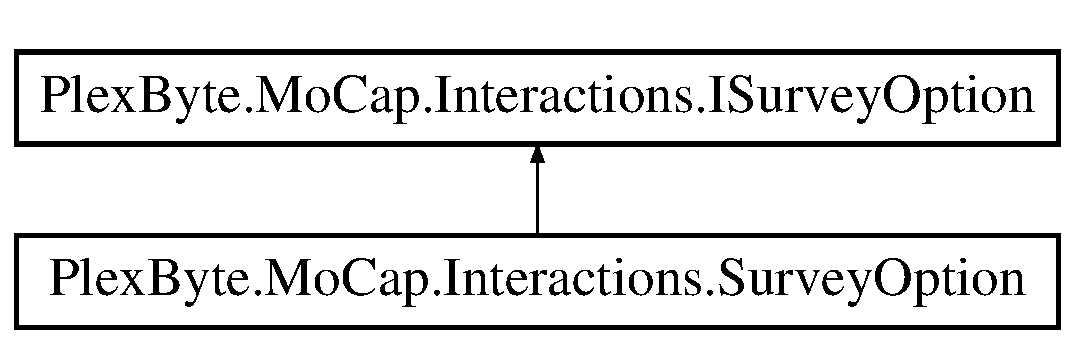
\includegraphics[height=2.000000cm]{class_plex_byte_1_1_mo_cap_1_1_interactions_1_1_survey_option}
\end{center}
\end{figure}
\subsection*{Public Member Functions}
\begin{DoxyCompactItemize}
\item 
\hyperlink{class_plex_byte_1_1_mo_cap_1_1_interactions_1_1_survey_option_ac4666dca9aede99181a51765fd0cd2bf}{Survey\+Option} (string p\+Id, string p\+Text)
\end{DoxyCompactItemize}
\subsection*{Properties}
\begin{DoxyCompactItemize}
\item 
Date\+Time \hyperlink{class_plex_byte_1_1_mo_cap_1_1_interactions_1_1_survey_option_a48d9a33c1256d0e03c9d2590af766865}{Created\+Date\+Time}\hspace{0.3cm}{\ttfamily  \mbox{[}get\mbox{]}}
\item 
string \hyperlink{class_plex_byte_1_1_mo_cap_1_1_interactions_1_1_survey_option_a9da80b0469096482b36fcfd126063d13}{Id}\hspace{0.3cm}{\ttfamily  \mbox{[}get\mbox{]}}
\item 
string \hyperlink{class_plex_byte_1_1_mo_cap_1_1_interactions_1_1_survey_option_a87cdd508f7cd9c80828c420486202bca}{Text}\hspace{0.3cm}{\ttfamily  \mbox{[}get\mbox{]}}
\end{DoxyCompactItemize}


\subsection{Detailed Description}
The survey option class, which hold the option text 



Definition at line 11 of file Survey\+Option.\+cs.



\subsection{Constructor \& Destructor Documentation}
\index{Plex\+Byte\+::\+Mo\+Cap\+::\+Interactions\+::\+Survey\+Option@{Plex\+Byte\+::\+Mo\+Cap\+::\+Interactions\+::\+Survey\+Option}!Survey\+Option@{Survey\+Option}}
\index{Survey\+Option@{Survey\+Option}!Plex\+Byte\+::\+Mo\+Cap\+::\+Interactions\+::\+Survey\+Option@{Plex\+Byte\+::\+Mo\+Cap\+::\+Interactions\+::\+Survey\+Option}}
\subsubsection[{\texorpdfstring{Survey\+Option(string p\+Id, string p\+Text)}{SurveyOption(string pId, string pText)}}]{\setlength{\rightskip}{0pt plus 5cm}Plex\+Byte.\+Mo\+Cap.\+Interactions.\+Survey\+Option.\+Survey\+Option (
\begin{DoxyParamCaption}
\item[{string}]{p\+Id, }
\item[{string}]{p\+Text}
\end{DoxyParamCaption}
)}\hypertarget{class_plex_byte_1_1_mo_cap_1_1_interactions_1_1_survey_option_ac4666dca9aede99181a51765fd0cd2bf}{}\label{class_plex_byte_1_1_mo_cap_1_1_interactions_1_1_survey_option_ac4666dca9aede99181a51765fd0cd2bf}


Definition at line 13 of file Survey\+Option.\+cs.



\subsection{Property Documentation}
\index{Plex\+Byte\+::\+Mo\+Cap\+::\+Interactions\+::\+Survey\+Option@{Plex\+Byte\+::\+Mo\+Cap\+::\+Interactions\+::\+Survey\+Option}!Created\+Date\+Time@{Created\+Date\+Time}}
\index{Created\+Date\+Time@{Created\+Date\+Time}!Plex\+Byte\+::\+Mo\+Cap\+::\+Interactions\+::\+Survey\+Option@{Plex\+Byte\+::\+Mo\+Cap\+::\+Interactions\+::\+Survey\+Option}}
\subsubsection[{\texorpdfstring{Created\+Date\+Time}{CreatedDateTime}}]{\setlength{\rightskip}{0pt plus 5cm}Date\+Time Plex\+Byte.\+Mo\+Cap.\+Interactions.\+Survey\+Option.\+Created\+Date\+Time\hspace{0.3cm}{\ttfamily [get]}}\hypertarget{class_plex_byte_1_1_mo_cap_1_1_interactions_1_1_survey_option_a48d9a33c1256d0e03c9d2590af766865}{}\label{class_plex_byte_1_1_mo_cap_1_1_interactions_1_1_survey_option_a48d9a33c1256d0e03c9d2590af766865}


Definition at line 20 of file Survey\+Option.\+cs.

\index{Plex\+Byte\+::\+Mo\+Cap\+::\+Interactions\+::\+Survey\+Option@{Plex\+Byte\+::\+Mo\+Cap\+::\+Interactions\+::\+Survey\+Option}!Id@{Id}}
\index{Id@{Id}!Plex\+Byte\+::\+Mo\+Cap\+::\+Interactions\+::\+Survey\+Option@{Plex\+Byte\+::\+Mo\+Cap\+::\+Interactions\+::\+Survey\+Option}}
\subsubsection[{\texorpdfstring{Id}{Id}}]{\setlength{\rightskip}{0pt plus 5cm}string Plex\+Byte.\+Mo\+Cap.\+Interactions.\+Survey\+Option.\+Id\hspace{0.3cm}{\ttfamily [get]}}\hypertarget{class_plex_byte_1_1_mo_cap_1_1_interactions_1_1_survey_option_a9da80b0469096482b36fcfd126063d13}{}\label{class_plex_byte_1_1_mo_cap_1_1_interactions_1_1_survey_option_a9da80b0469096482b36fcfd126063d13}


Definition at line 22 of file Survey\+Option.\+cs.

\index{Plex\+Byte\+::\+Mo\+Cap\+::\+Interactions\+::\+Survey\+Option@{Plex\+Byte\+::\+Mo\+Cap\+::\+Interactions\+::\+Survey\+Option}!Text@{Text}}
\index{Text@{Text}!Plex\+Byte\+::\+Mo\+Cap\+::\+Interactions\+::\+Survey\+Option@{Plex\+Byte\+::\+Mo\+Cap\+::\+Interactions\+::\+Survey\+Option}}
\subsubsection[{\texorpdfstring{Text}{Text}}]{\setlength{\rightskip}{0pt plus 5cm}string Plex\+Byte.\+Mo\+Cap.\+Interactions.\+Survey\+Option.\+Text\hspace{0.3cm}{\ttfamily [get]}}\hypertarget{class_plex_byte_1_1_mo_cap_1_1_interactions_1_1_survey_option_a87cdd508f7cd9c80828c420486202bca}{}\label{class_plex_byte_1_1_mo_cap_1_1_interactions_1_1_survey_option_a87cdd508f7cd9c80828c420486202bca}


Definition at line 24 of file Survey\+Option.\+cs.



The documentation for this class was generated from the following file\+:\begin{DoxyCompactItemize}
\item 
D\+:/\+Users/\+Christian\+B/\+Documents/\+\_\+\+H\+F Infomatik/\+Git\+Hub\+\_\+\+Repos/\+Mo\+Cap/\+Plex\+Byte.\+Mo\+Cap/\+Plex\+Byte.\+Mo\+Cap.\+Interactions/\hyperlink{_survey_option_8cs}{Survey\+Option.\+cs}\end{DoxyCompactItemize}

\hypertarget{class_plex_byte_1_1_mo_cap_1_1_interactions_1_1_task}{}\section{Plex\+Byte.\+Mo\+Cap.\+Interactions.\+Task Class Reference}
\label{class_plex_byte_1_1_mo_cap_1_1_interactions_1_1_task}\index{Plex\+Byte.\+Mo\+Cap.\+Interactions.\+Task@{Plex\+Byte.\+Mo\+Cap.\+Interactions.\+Task}}
Inheritance diagram for Plex\+Byte.\+Mo\+Cap.\+Interactions.\+Task\+:\begin{figure}[H]
\begin{center}
\leavevmode
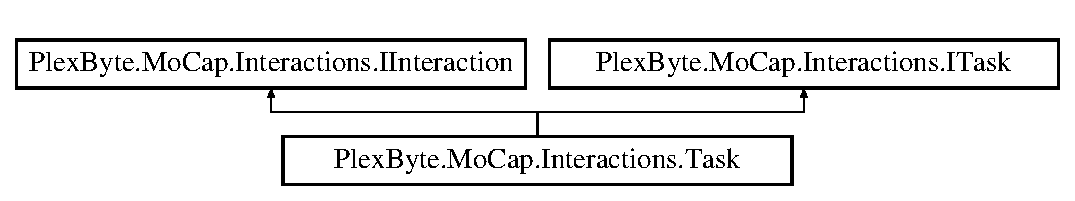
\includegraphics[height=2.000000cm]{class_plex_byte_1_1_mo_cap_1_1_interactions_1_1_task}
\end{center}
\end{figure}
\subsection*{Public Member Functions}
\begin{DoxyCompactItemize}
\item 
delegate void \hyperlink{class_plex_byte_1_1_mo_cap_1_1_interactions_1_1_task_a7a8fb4764f97d4221d9c01f36737350e}{Progress\+Update} (object sender, \hyperlink{class_plex_byte_1_1_mo_cap_1_1_interactions_1_1_interaction_event_args}{Interaction\+Event\+Args} e)
\item 
\hyperlink{class_plex_byte_1_1_mo_cap_1_1_interactions_1_1_task_a57a0376ee5adf1aa90a555a5e3e1a90e}{Task} (string p\+Id, string p\+Text, I\+User p\+Creator)
\item 
\hyperlink{class_plex_byte_1_1_mo_cap_1_1_interactions_1_1_task_ad7b0d80dfd8588bcae2b8b90404b279f}{Task} (string p\+Id, string p\+Text, I\+User p\+Creator, Date\+Time p\+Start\+Dt, Date\+Time p\+End\+Dt, Date\+Time p\+Due\+Dt)
\item 
\hyperlink{class_plex_byte_1_1_mo_cap_1_1_interactions_1_1_task_a7646af76da19c1b8f96d216ae76f6ed8}{Task} (string p\+Id, string p\+Text, string p\+Title, I\+User p\+Creator, Date\+Time p\+Start\+Dt, Date\+Time p\+End\+Dt, Date\+Time p\+Due\+Dt, decimal p\+Budget, int p\+Duration, int p\+Priority, \hyperlink{namespace_plex_byte_1_1_mo_cap_1_1_interactions_afcb673d9186608b6bd3b187179aedc8a}{Interaction\+State} p\+State, decimal p\+Budget\+Used, int p\+Time\+Used, List$<$ \hyperlink{interface_plex_byte_1_1_mo_cap_1_1_interactions_1_1_i_task}{I\+Task} $>$ p\+Sub\+Task, int p\+Progress)
\item 
virtual void \hyperlink{class_plex_byte_1_1_mo_cap_1_1_interactions_1_1_task_ab74ee9d89534254215ae13eb91e12227}{On\+Complete} (\hyperlink{class_plex_byte_1_1_mo_cap_1_1_interactions_1_1_interaction_event_args}{Interaction\+Event\+Args} p\+Event\+Args)
\item 
void \hyperlink{class_plex_byte_1_1_mo_cap_1_1_interactions_1_1_task_a94296d62be4af091fd6a5e9a8a0fde8a}{On\+State\+Changed} (\hyperlink{class_plex_byte_1_1_mo_cap_1_1_interactions_1_1_interaction_event_args}{Interaction\+Event\+Args} p\+Event\+Args)
\item 
virtual void \hyperlink{class_plex_byte_1_1_mo_cap_1_1_interactions_1_1_task_ae9e732dc2f41a35a77dd8e143c8cf9c7}{On\+Modify} (\hyperlink{class_plex_byte_1_1_mo_cap_1_1_interactions_1_1_interaction_event_args}{Interaction\+Event\+Args} p\+Event\+Args)
\item 
virtual void \hyperlink{class_plex_byte_1_1_mo_cap_1_1_interactions_1_1_task_a47eac360e6cf4cd6b84f7445ee4a6a33}{Change\+Owner} (I\+User p\+User)
\item 
virtual void \hyperlink{class_plex_byte_1_1_mo_cap_1_1_interactions_1_1_task_ae0cb74071fbffd9fa7cd1dba842b6715}{Change\+Is\+Active} (bool p\+Active)
\item 
virtual void \hyperlink{class_plex_byte_1_1_mo_cap_1_1_interactions_1_1_task_ab8d71506e5343bc302bb661a5131449b}{Add\+Timeslice} (int p\+Duration)
\item 
virtual void \hyperlink{class_plex_byte_1_1_mo_cap_1_1_interactions_1_1_task_a12136bc5d5722e10c4a20b4e9ab40788}{Add\+Expense} (decimal p\+Expense\+Value)
\item 
void \hyperlink{class_plex_byte_1_1_mo_cap_1_1_interactions_1_1_task_a42cc4439fb4ab6d4e11f8764b217b46d}{Change\+State} (\hyperlink{namespace_plex_byte_1_1_mo_cap_1_1_interactions_afcb673d9186608b6bd3b187179aedc8a}{Interaction\+State} p\+State)
\item 
void \hyperlink{class_plex_byte_1_1_mo_cap_1_1_interactions_1_1_task_aa152325c4d018f68b8dcbe1ef4c46497}{Add\+Sub\+Task} (\hyperlink{interface_plex_byte_1_1_mo_cap_1_1_interactions_1_1_i_task}{I\+Task} p\+Task)
\item 
void \hyperlink{class_plex_byte_1_1_mo_cap_1_1_interactions_1_1_task_af28b4349816bcd4d60c0746e7b7425d4}{Udate\+Progress} (int p\+Progress)
\end{DoxyCompactItemize}
\subsection*{Public Attributes}
\begin{DoxyCompactItemize}
\item 
string \hyperlink{class_plex_byte_1_1_mo_cap_1_1_interactions_1_1_task_a56373e896c8d387f53b89c820b78686c}{Id} =$>$ \+\_\+id
\begin{DoxyCompactList}\small\item\em The unique id of the task \end{DoxyCompactList}\item 
Date\+Time \hyperlink{class_plex_byte_1_1_mo_cap_1_1_interactions_1_1_task_ad09e75c883291d7bf2a5be651c2e48f5}{Created\+Date\+Time} =$>$ \+\_\+created\+Date\+Time
\begin{DoxyCompactList}\small\item\em The date and time the task was created \end{DoxyCompactList}\item 
bool \hyperlink{class_plex_byte_1_1_mo_cap_1_1_interactions_1_1_task_a4e3e7f12d9ebbef619979f8aa1debaa9}{Is\+Active} =$>$ \+\_\+is\+Active
\begin{DoxyCompactList}\small\item\em Flag indicating whether or not the task can be worked on \end{DoxyCompactList}\item 
I\+User \hyperlink{class_plex_byte_1_1_mo_cap_1_1_interactions_1_1_task_a8fbe07ee1d4f0d20465aa6eb78dd5959}{Creator} =$>$ \+\_\+creator
\begin{DoxyCompactList}\small\item\em The user that created the task \end{DoxyCompactList}\item 
\hyperlink{namespace_plex_byte_1_1_mo_cap_1_1_interactions_afcb673d9186608b6bd3b187179aedc8a}{Interaction\+State} \hyperlink{class_plex_byte_1_1_mo_cap_1_1_interactions_1_1_task_ade847c2f68b897a4eae7463134aadaa1}{State} =$>$ \+\_\+state
\begin{DoxyCompactList}\small\item\em The state of the task \end{DoxyCompactList}\item 
decimal \hyperlink{class_plex_byte_1_1_mo_cap_1_1_interactions_1_1_task_a754524cdae030db2de7d38cae665ed7e}{Budget} =$>$ \+\_\+budget
\begin{DoxyCompactList}\small\item\em The tasks budget \end{DoxyCompactList}\item 
int \hyperlink{class_plex_byte_1_1_mo_cap_1_1_interactions_1_1_task_a84a9a89d90c83269366f70ea3e6cc2b9}{Duration} =$>$ \+\_\+duration
\begin{DoxyCompactList}\small\item\em The task duration in seconds \end{DoxyCompactList}\item 
int \hyperlink{class_plex_byte_1_1_mo_cap_1_1_interactions_1_1_task_a4b3325d26ed2025dd44f597a428cfdd0}{Priority} =$>$ \+\_\+priority
\begin{DoxyCompactList}\small\item\em The priority of this task \end{DoxyCompactList}\item 
List$<$ \hyperlink{interface_plex_byte_1_1_mo_cap_1_1_interactions_1_1_i_task}{I\+Task} $>$ \hyperlink{class_plex_byte_1_1_mo_cap_1_1_interactions_1_1_task_adc2d20b794d9621f0f9496d753376a92}{Sub\+Tasks} =$>$ \+\_\+sub\+Tasks
\begin{DoxyCompactList}\small\item\em The list of sub tasks assigned \end{DoxyCompactList}\item 
int \hyperlink{class_plex_byte_1_1_mo_cap_1_1_interactions_1_1_task_a557416cee8b3425c49f40fc07435719e}{Progress} =$>$ \+\_\+progress
\begin{DoxyCompactList}\small\item\em The progresss of the task \end{DoxyCompactList}\item 
Date\+Time \hyperlink{class_plex_byte_1_1_mo_cap_1_1_interactions_1_1_task_ad232b867da717b3f823363d627b24009}{Due\+Date\+Time} =$>$ \+\_\+due\+Date\+Time
\end{DoxyCompactItemize}
\subsection*{Protected Member Functions}
\begin{DoxyCompactItemize}
\item 
virtual void \hyperlink{class_plex_byte_1_1_mo_cap_1_1_interactions_1_1_task_a9784fcd7276f0b4111d7a7f8ef64e34e}{On\+Progress\+Updated} (\hyperlink{class_plex_byte_1_1_mo_cap_1_1_interactions_1_1_interaction_event_args}{Interaction\+Event\+Args} e)
\end{DoxyCompactItemize}
\subsection*{Properties}
\begin{DoxyCompactItemize}
\item 
string \hyperlink{class_plex_byte_1_1_mo_cap_1_1_interactions_1_1_task_a1e0a8c220a72fc6189fa7081e6279a67}{Interaction\+Id}\hspace{0.3cm}{\ttfamily  \mbox{[}get, set\mbox{]}}
\item 
string \hyperlink{class_plex_byte_1_1_mo_cap_1_1_interactions_1_1_task_a5827bb9ca244149e76780756ce196057}{Project\+Id}\hspace{0.3cm}{\ttfamily  \mbox{[}get, set\mbox{]}}
\item 
Date\+Time \hyperlink{class_plex_byte_1_1_mo_cap_1_1_interactions_1_1_task_a3b4287e83b9825d68a583ad68ec60b65}{Start\+Date\+Time}\hspace{0.3cm}{\ttfamily  \mbox{[}get, set\mbox{]}}
\begin{DoxyCompactList}\small\item\em The date and time this task becomes active and can be worked on. As long as this date is not reached the state will remain queued and no work can be performed on the task as longs as it is in state queued \end{DoxyCompactList}\item 
Date\+Time \hyperlink{class_plex_byte_1_1_mo_cap_1_1_interactions_1_1_task_a7855e576032a285a50f918098e030c7f}{End\+Date\+Time}\hspace{0.3cm}{\ttfamily  \mbox{[}get, set\mbox{]}}
\begin{DoxyCompactList}\small\item\em The date and time this task should be finished. If this date is reached the state will change to expired \end{DoxyCompactList}\item 
Date\+Time \hyperlink{class_plex_byte_1_1_mo_cap_1_1_interactions_1_1_task_aea629926c184e80ae57914422f5fcb4c}{Modified\+Date\+Time}\hspace{0.3cm}{\ttfamily  \mbox{[}get, set\mbox{]}}
\begin{DoxyCompactList}\small\item\em The date and time the task was last modified \end{DoxyCompactList}\item 
string \hyperlink{class_plex_byte_1_1_mo_cap_1_1_interactions_1_1_task_afc2aa1b0a8699fe0a607b452eb5461c3}{Title}\hspace{0.3cm}{\ttfamily  \mbox{[}get, set\mbox{]}}
\item 
string \hyperlink{class_plex_byte_1_1_mo_cap_1_1_interactions_1_1_task_ad80addfa475e483ae816bbd1bd199bf9}{Text}\hspace{0.3cm}{\ttfamily  \mbox{[}get, set\mbox{]}}
\begin{DoxyCompactList}\small\item\em The text of this task (description) \end{DoxyCompactList}\item 
\hyperlink{namespace_plex_byte_1_1_mo_cap_1_1_interactions_a6e7bea333446664bbce2bb296db25e31}{Interaction\+Type} \hyperlink{class_plex_byte_1_1_mo_cap_1_1_interactions_1_1_task_a8d56efe5c3efeb4df5f291cac8a57128}{Type}\hspace{0.3cm}{\ttfamily  \mbox{[}get\mbox{]}}
\begin{DoxyCompactList}\small\item\em The type of interaction (will be always task) \end{DoxyCompactList}\item 
I\+User \hyperlink{class_plex_byte_1_1_mo_cap_1_1_interactions_1_1_task_a3cdc15c2ceb9683e5b19d76462a5fb21}{Owner}\hspace{0.3cm}{\ttfamily  \mbox{[}get, set\mbox{]}}
\begin{DoxyCompactList}\small\item\em The user currently owning the task \end{DoxyCompactList}\item 
int \hyperlink{class_plex_byte_1_1_mo_cap_1_1_interactions_1_1_task_a0f087ca6c9a9af79cddb8c409f810526}{Duration\+Current}\hspace{0.3cm}{\ttfamily  \mbox{[}get\mbox{]}}
\begin{DoxyCompactList}\small\item\em The time currently spent on this task in seconds \end{DoxyCompactList}\item 
decimal \hyperlink{class_plex_byte_1_1_mo_cap_1_1_interactions_1_1_task_a982a30703b7b2c3258adad8e09a1ea29}{Budget\+Used} = 0\hspace{0.3cm}{\ttfamily  \mbox{[}get\mbox{]}}
\begin{DoxyCompactList}\small\item\em The investment currently made in this task \end{DoxyCompactList}\end{DoxyCompactItemize}
\subsection*{Events}
\begin{DoxyCompactItemize}
\item 
\hyperlink{namespace_plex_byte_1_1_mo_cap_1_1_interactions_ac81ac3321ab2b018c75ad2c18ec15b9e}{Complete} \hyperlink{class_plex_byte_1_1_mo_cap_1_1_interactions_1_1_task_a0d4c6a5a630e50b403c7e767d970206f}{Completed}
\item 
\hyperlink{namespace_plex_byte_1_1_mo_cap_1_1_interactions_a490186f613e46adce26244f3b2c78a58}{Modify} \hyperlink{class_plex_byte_1_1_mo_cap_1_1_interactions_1_1_task_a84fdfe29a8cd9889cd2eb0d2216d01d1}{Modified}
\item 
\hyperlink{namespace_plex_byte_1_1_mo_cap_1_1_interactions_af2ff213e81451f96fc74bfad114cecde}{State\+Change} \hyperlink{class_plex_byte_1_1_mo_cap_1_1_interactions_1_1_task_ad95c06276af6eb715b37421f1a121cc8}{State\+Changed}
\item 
\hyperlink{class_plex_byte_1_1_mo_cap_1_1_interactions_1_1_task_a7a8fb4764f97d4221d9c01f36737350e}{Progress\+Update} \hyperlink{class_plex_byte_1_1_mo_cap_1_1_interactions_1_1_task_a018dbc01193478565a41d56409618e9a}{Progress\+Updated}
\end{DoxyCompactItemize}


\subsection{Detailed Description}


Definition at line 13 of file Task.\+cs.



\subsection{Constructor \& Destructor Documentation}
\index{Plex\+Byte\+::\+Mo\+Cap\+::\+Interactions\+::\+Task@{Plex\+Byte\+::\+Mo\+Cap\+::\+Interactions\+::\+Task}!Task@{Task}}
\index{Task@{Task}!Plex\+Byte\+::\+Mo\+Cap\+::\+Interactions\+::\+Task@{Plex\+Byte\+::\+Mo\+Cap\+::\+Interactions\+::\+Task}}
\subsubsection[{\texorpdfstring{Task(string p\+Id, string p\+Text, I\+User p\+Creator)}{Task(string pId, string pText, IUser pCreator)}}]{\setlength{\rightskip}{0pt plus 5cm}Plex\+Byte.\+Mo\+Cap.\+Interactions.\+Task.\+Task (
\begin{DoxyParamCaption}
\item[{string}]{p\+Id, }
\item[{string}]{p\+Text, }
\item[{I\+User}]{p\+Creator}
\end{DoxyParamCaption}
)}\hypertarget{class_plex_byte_1_1_mo_cap_1_1_interactions_1_1_task_a57a0376ee5adf1aa90a555a5e3e1a90e}{}\label{class_plex_byte_1_1_mo_cap_1_1_interactions_1_1_task_a57a0376ee5adf1aa90a555a5e3e1a90e}


Definition at line 156 of file Task.\+cs.

\index{Plex\+Byte\+::\+Mo\+Cap\+::\+Interactions\+::\+Task@{Plex\+Byte\+::\+Mo\+Cap\+::\+Interactions\+::\+Task}!Task@{Task}}
\index{Task@{Task}!Plex\+Byte\+::\+Mo\+Cap\+::\+Interactions\+::\+Task@{Plex\+Byte\+::\+Mo\+Cap\+::\+Interactions\+::\+Task}}
\subsubsection[{\texorpdfstring{Task(string p\+Id, string p\+Text, I\+User p\+Creator, Date\+Time p\+Start\+Dt, Date\+Time p\+End\+Dt, Date\+Time p\+Due\+Dt)}{Task(string pId, string pText, IUser pCreator, DateTime pStartDt, DateTime pEndDt, DateTime pDueDt)}}]{\setlength{\rightskip}{0pt plus 5cm}Plex\+Byte.\+Mo\+Cap.\+Interactions.\+Task.\+Task (
\begin{DoxyParamCaption}
\item[{string}]{p\+Id, }
\item[{string}]{p\+Text, }
\item[{I\+User}]{p\+Creator, }
\item[{Date\+Time}]{p\+Start\+Dt, }
\item[{Date\+Time}]{p\+End\+Dt, }
\item[{Date\+Time}]{p\+Due\+Dt}
\end{DoxyParamCaption}
)}\hypertarget{class_plex_byte_1_1_mo_cap_1_1_interactions_1_1_task_ad7b0d80dfd8588bcae2b8b90404b279f}{}\label{class_plex_byte_1_1_mo_cap_1_1_interactions_1_1_task_ad7b0d80dfd8588bcae2b8b90404b279f}


Definition at line 175 of file Task.\+cs.

\index{Plex\+Byte\+::\+Mo\+Cap\+::\+Interactions\+::\+Task@{Plex\+Byte\+::\+Mo\+Cap\+::\+Interactions\+::\+Task}!Task@{Task}}
\index{Task@{Task}!Plex\+Byte\+::\+Mo\+Cap\+::\+Interactions\+::\+Task@{Plex\+Byte\+::\+Mo\+Cap\+::\+Interactions\+::\+Task}}
\subsubsection[{\texorpdfstring{Task(string p\+Id, string p\+Text, string p\+Title, I\+User p\+Creator, Date\+Time p\+Start\+Dt, Date\+Time p\+End\+Dt, Date\+Time p\+Due\+Dt, decimal p\+Budget, int p\+Duration, int p\+Priority, Interaction\+State p\+State, decimal p\+Budget\+Used, int p\+Time\+Used, List$<$ I\+Task $>$ p\+Sub\+Task, int p\+Progress)}{Task(string pId, string pText, string pTitle, IUser pCreator, DateTime pStartDt, DateTime pEndDt, DateTime pDueDt, decimal pBudget, int pDuration, int pPriority, InteractionState pState, decimal pBudgetUsed, int pTimeUsed, List< ITask > pSubTask, int pProgress)}}]{\setlength{\rightskip}{0pt plus 5cm}Plex\+Byte.\+Mo\+Cap.\+Interactions.\+Task.\+Task (
\begin{DoxyParamCaption}
\item[{string}]{p\+Id, }
\item[{string}]{p\+Text, }
\item[{string}]{p\+Title, }
\item[{I\+User}]{p\+Creator, }
\item[{Date\+Time}]{p\+Start\+Dt, }
\item[{Date\+Time}]{p\+End\+Dt, }
\item[{Date\+Time}]{p\+Due\+Dt, }
\item[{decimal}]{p\+Budget, }
\item[{int}]{p\+Duration, }
\item[{int}]{p\+Priority, }
\item[{{\bf Interaction\+State}}]{p\+State, }
\item[{decimal}]{p\+Budget\+Used, }
\item[{int}]{p\+Time\+Used, }
\item[{List$<$ {\bf I\+Task} $>$}]{p\+Sub\+Task, }
\item[{int}]{p\+Progress}
\end{DoxyParamCaption}
)}\hypertarget{class_plex_byte_1_1_mo_cap_1_1_interactions_1_1_task_a7646af76da19c1b8f96d216ae76f6ed8}{}\label{class_plex_byte_1_1_mo_cap_1_1_interactions_1_1_task_a7646af76da19c1b8f96d216ae76f6ed8}


Definition at line 194 of file Task.\+cs.



\subsection{Member Function Documentation}
\index{Plex\+Byte\+::\+Mo\+Cap\+::\+Interactions\+::\+Task@{Plex\+Byte\+::\+Mo\+Cap\+::\+Interactions\+::\+Task}!Add\+Expense@{Add\+Expense}}
\index{Add\+Expense@{Add\+Expense}!Plex\+Byte\+::\+Mo\+Cap\+::\+Interactions\+::\+Task@{Plex\+Byte\+::\+Mo\+Cap\+::\+Interactions\+::\+Task}}
\subsubsection[{\texorpdfstring{Add\+Expense(decimal p\+Expense\+Value)}{AddExpense(decimal pExpenseValue)}}]{\setlength{\rightskip}{0pt plus 5cm}virtual void Plex\+Byte.\+Mo\+Cap.\+Interactions.\+Task.\+Add\+Expense (
\begin{DoxyParamCaption}
\item[{decimal}]{p\+Expense\+Value}
\end{DoxyParamCaption}
)\hspace{0.3cm}{\ttfamily [virtual]}}\hypertarget{class_plex_byte_1_1_mo_cap_1_1_interactions_1_1_task_a12136bc5d5722e10c4a20b4e9ab40788}{}\label{class_plex_byte_1_1_mo_cap_1_1_interactions_1_1_task_a12136bc5d5722e10c4a20b4e9ab40788}


Implements \hyperlink{interface_plex_byte_1_1_mo_cap_1_1_interactions_1_1_i_task_a96b54ce198b08eccb95456e16c4538d5}{Plex\+Byte.\+Mo\+Cap.\+Interactions.\+I\+Task}.



Definition at line 283 of file Task.\+cs.

\index{Plex\+Byte\+::\+Mo\+Cap\+::\+Interactions\+::\+Task@{Plex\+Byte\+::\+Mo\+Cap\+::\+Interactions\+::\+Task}!Add\+Sub\+Task@{Add\+Sub\+Task}}
\index{Add\+Sub\+Task@{Add\+Sub\+Task}!Plex\+Byte\+::\+Mo\+Cap\+::\+Interactions\+::\+Task@{Plex\+Byte\+::\+Mo\+Cap\+::\+Interactions\+::\+Task}}
\subsubsection[{\texorpdfstring{Add\+Sub\+Task(\+I\+Task p\+Task)}{AddSubTask(ITask pTask)}}]{\setlength{\rightskip}{0pt plus 5cm}void Plex\+Byte.\+Mo\+Cap.\+Interactions.\+Task.\+Add\+Sub\+Task (
\begin{DoxyParamCaption}
\item[{{\bf I\+Task}}]{p\+Task}
\end{DoxyParamCaption}
)}\hypertarget{class_plex_byte_1_1_mo_cap_1_1_interactions_1_1_task_aa152325c4d018f68b8dcbe1ef4c46497}{}\label{class_plex_byte_1_1_mo_cap_1_1_interactions_1_1_task_aa152325c4d018f68b8dcbe1ef4c46497}


Implements \hyperlink{interface_plex_byte_1_1_mo_cap_1_1_interactions_1_1_i_task_a20a23d8d8abb9f14330e75e8e09fe263}{Plex\+Byte.\+Mo\+Cap.\+Interactions.\+I\+Task}.



Definition at line 317 of file Task.\+cs.

\index{Plex\+Byte\+::\+Mo\+Cap\+::\+Interactions\+::\+Task@{Plex\+Byte\+::\+Mo\+Cap\+::\+Interactions\+::\+Task}!Add\+Timeslice@{Add\+Timeslice}}
\index{Add\+Timeslice@{Add\+Timeslice}!Plex\+Byte\+::\+Mo\+Cap\+::\+Interactions\+::\+Task@{Plex\+Byte\+::\+Mo\+Cap\+::\+Interactions\+::\+Task}}
\subsubsection[{\texorpdfstring{Add\+Timeslice(int p\+Duration)}{AddTimeslice(int pDuration)}}]{\setlength{\rightskip}{0pt plus 5cm}virtual void Plex\+Byte.\+Mo\+Cap.\+Interactions.\+Task.\+Add\+Timeslice (
\begin{DoxyParamCaption}
\item[{int}]{p\+Duration}
\end{DoxyParamCaption}
)\hspace{0.3cm}{\ttfamily [virtual]}}\hypertarget{class_plex_byte_1_1_mo_cap_1_1_interactions_1_1_task_ab8d71506e5343bc302bb661a5131449b}{}\label{class_plex_byte_1_1_mo_cap_1_1_interactions_1_1_task_ab8d71506e5343bc302bb661a5131449b}


Implements \hyperlink{interface_plex_byte_1_1_mo_cap_1_1_interactions_1_1_i_task_af70a3a36f24fedda95ad55714333090f}{Plex\+Byte.\+Mo\+Cap.\+Interactions.\+I\+Task}.



Definition at line 272 of file Task.\+cs.

\index{Plex\+Byte\+::\+Mo\+Cap\+::\+Interactions\+::\+Task@{Plex\+Byte\+::\+Mo\+Cap\+::\+Interactions\+::\+Task}!Change\+Is\+Active@{Change\+Is\+Active}}
\index{Change\+Is\+Active@{Change\+Is\+Active}!Plex\+Byte\+::\+Mo\+Cap\+::\+Interactions\+::\+Task@{Plex\+Byte\+::\+Mo\+Cap\+::\+Interactions\+::\+Task}}
\subsubsection[{\texorpdfstring{Change\+Is\+Active(bool p\+Active)}{ChangeIsActive(bool pActive)}}]{\setlength{\rightskip}{0pt plus 5cm}virtual void Plex\+Byte.\+Mo\+Cap.\+Interactions.\+Task.\+Change\+Is\+Active (
\begin{DoxyParamCaption}
\item[{bool}]{p\+Active}
\end{DoxyParamCaption}
)\hspace{0.3cm}{\ttfamily [virtual]}}\hypertarget{class_plex_byte_1_1_mo_cap_1_1_interactions_1_1_task_ae0cb74071fbffd9fa7cd1dba842b6715}{}\label{class_plex_byte_1_1_mo_cap_1_1_interactions_1_1_task_ae0cb74071fbffd9fa7cd1dba842b6715}


Implements \hyperlink{interface_plex_byte_1_1_mo_cap_1_1_interactions_1_1_i_interaction_ac2d9f47a1139b931939e8cff07153aba}{Plex\+Byte.\+Mo\+Cap.\+Interactions.\+I\+Interaction}.



Definition at line 256 of file Task.\+cs.

\index{Plex\+Byte\+::\+Mo\+Cap\+::\+Interactions\+::\+Task@{Plex\+Byte\+::\+Mo\+Cap\+::\+Interactions\+::\+Task}!Change\+Owner@{Change\+Owner}}
\index{Change\+Owner@{Change\+Owner}!Plex\+Byte\+::\+Mo\+Cap\+::\+Interactions\+::\+Task@{Plex\+Byte\+::\+Mo\+Cap\+::\+Interactions\+::\+Task}}
\subsubsection[{\texorpdfstring{Change\+Owner(\+I\+User p\+User)}{ChangeOwner(IUser pUser)}}]{\setlength{\rightskip}{0pt plus 5cm}virtual void Plex\+Byte.\+Mo\+Cap.\+Interactions.\+Task.\+Change\+Owner (
\begin{DoxyParamCaption}
\item[{I\+User}]{p\+User}
\end{DoxyParamCaption}
)\hspace{0.3cm}{\ttfamily [virtual]}}\hypertarget{class_plex_byte_1_1_mo_cap_1_1_interactions_1_1_task_a47eac360e6cf4cd6b84f7445ee4a6a33}{}\label{class_plex_byte_1_1_mo_cap_1_1_interactions_1_1_task_a47eac360e6cf4cd6b84f7445ee4a6a33}


Implements \hyperlink{interface_plex_byte_1_1_mo_cap_1_1_interactions_1_1_i_interaction_a7e3b0a67dc7d176877b8b94922a9bb52}{Plex\+Byte.\+Mo\+Cap.\+Interactions.\+I\+Interaction}.



Definition at line 246 of file Task.\+cs.

\index{Plex\+Byte\+::\+Mo\+Cap\+::\+Interactions\+::\+Task@{Plex\+Byte\+::\+Mo\+Cap\+::\+Interactions\+::\+Task}!Change\+State@{Change\+State}}
\index{Change\+State@{Change\+State}!Plex\+Byte\+::\+Mo\+Cap\+::\+Interactions\+::\+Task@{Plex\+Byte\+::\+Mo\+Cap\+::\+Interactions\+::\+Task}}
\subsubsection[{\texorpdfstring{Change\+State(\+Interaction\+State p\+State)}{ChangeState(InteractionState pState)}}]{\setlength{\rightskip}{0pt plus 5cm}void Plex\+Byte.\+Mo\+Cap.\+Interactions.\+Task.\+Change\+State (
\begin{DoxyParamCaption}
\item[{{\bf Interaction\+State}}]{p\+State}
\end{DoxyParamCaption}
)}\hypertarget{class_plex_byte_1_1_mo_cap_1_1_interactions_1_1_task_a42cc4439fb4ab6d4e11f8764b217b46d}{}\label{class_plex_byte_1_1_mo_cap_1_1_interactions_1_1_task_a42cc4439fb4ab6d4e11f8764b217b46d}


Implements \hyperlink{interface_plex_byte_1_1_mo_cap_1_1_interactions_1_1_i_interaction_a10beb35eb6061878469b5a6cd5431b32}{Plex\+Byte.\+Mo\+Cap.\+Interactions.\+I\+Interaction}.



Definition at line 294 of file Task.\+cs.

\index{Plex\+Byte\+::\+Mo\+Cap\+::\+Interactions\+::\+Task@{Plex\+Byte\+::\+Mo\+Cap\+::\+Interactions\+::\+Task}!On\+Complete@{On\+Complete}}
\index{On\+Complete@{On\+Complete}!Plex\+Byte\+::\+Mo\+Cap\+::\+Interactions\+::\+Task@{Plex\+Byte\+::\+Mo\+Cap\+::\+Interactions\+::\+Task}}
\subsubsection[{\texorpdfstring{On\+Complete(\+Interaction\+Event\+Args p\+Event\+Args)}{OnComplete(InteractionEventArgs pEventArgs)}}]{\setlength{\rightskip}{0pt plus 5cm}virtual void Plex\+Byte.\+Mo\+Cap.\+Interactions.\+Task.\+On\+Complete (
\begin{DoxyParamCaption}
\item[{{\bf Interaction\+Event\+Args}}]{p\+Event\+Args}
\end{DoxyParamCaption}
)\hspace{0.3cm}{\ttfamily [virtual]}}\hypertarget{class_plex_byte_1_1_mo_cap_1_1_interactions_1_1_task_ab74ee9d89534254215ae13eb91e12227}{}\label{class_plex_byte_1_1_mo_cap_1_1_interactions_1_1_task_ab74ee9d89534254215ae13eb91e12227}


Implements \hyperlink{interface_plex_byte_1_1_mo_cap_1_1_interactions_1_1_i_interaction_a9f32d6c1c2f2ae60dabb274f62128447}{Plex\+Byte.\+Mo\+Cap.\+Interactions.\+I\+Interaction}.



Definition at line 234 of file Task.\+cs.

\index{Plex\+Byte\+::\+Mo\+Cap\+::\+Interactions\+::\+Task@{Plex\+Byte\+::\+Mo\+Cap\+::\+Interactions\+::\+Task}!On\+Modify@{On\+Modify}}
\index{On\+Modify@{On\+Modify}!Plex\+Byte\+::\+Mo\+Cap\+::\+Interactions\+::\+Task@{Plex\+Byte\+::\+Mo\+Cap\+::\+Interactions\+::\+Task}}
\subsubsection[{\texorpdfstring{On\+Modify(\+Interaction\+Event\+Args p\+Event\+Args)}{OnModify(InteractionEventArgs pEventArgs)}}]{\setlength{\rightskip}{0pt plus 5cm}virtual void Plex\+Byte.\+Mo\+Cap.\+Interactions.\+Task.\+On\+Modify (
\begin{DoxyParamCaption}
\item[{{\bf Interaction\+Event\+Args}}]{p\+Event\+Args}
\end{DoxyParamCaption}
)\hspace{0.3cm}{\ttfamily [virtual]}}\hypertarget{class_plex_byte_1_1_mo_cap_1_1_interactions_1_1_task_ae9e732dc2f41a35a77dd8e143c8cf9c7}{}\label{class_plex_byte_1_1_mo_cap_1_1_interactions_1_1_task_ae9e732dc2f41a35a77dd8e143c8cf9c7}


Implements \hyperlink{interface_plex_byte_1_1_mo_cap_1_1_interactions_1_1_i_interaction_af4fac42d753ae7f9652541542b8961c6}{Plex\+Byte.\+Mo\+Cap.\+Interactions.\+I\+Interaction}.



Definition at line 238 of file Task.\+cs.

\index{Plex\+Byte\+::\+Mo\+Cap\+::\+Interactions\+::\+Task@{Plex\+Byte\+::\+Mo\+Cap\+::\+Interactions\+::\+Task}!On\+Progress\+Updated@{On\+Progress\+Updated}}
\index{On\+Progress\+Updated@{On\+Progress\+Updated}!Plex\+Byte\+::\+Mo\+Cap\+::\+Interactions\+::\+Task@{Plex\+Byte\+::\+Mo\+Cap\+::\+Interactions\+::\+Task}}
\subsubsection[{\texorpdfstring{On\+Progress\+Updated(\+Interaction\+Event\+Args e)}{OnProgressUpdated(InteractionEventArgs e)}}]{\setlength{\rightskip}{0pt plus 5cm}virtual void Plex\+Byte.\+Mo\+Cap.\+Interactions.\+Task.\+On\+Progress\+Updated (
\begin{DoxyParamCaption}
\item[{{\bf Interaction\+Event\+Args}}]{e}
\end{DoxyParamCaption}
)\hspace{0.3cm}{\ttfamily [protected]}, {\ttfamily [virtual]}}\hypertarget{class_plex_byte_1_1_mo_cap_1_1_interactions_1_1_task_a9784fcd7276f0b4111d7a7f8ef64e34e}{}\label{class_plex_byte_1_1_mo_cap_1_1_interactions_1_1_task_a9784fcd7276f0b4111d7a7f8ef64e34e}


Definition at line 240 of file Task.\+cs.

\index{Plex\+Byte\+::\+Mo\+Cap\+::\+Interactions\+::\+Task@{Plex\+Byte\+::\+Mo\+Cap\+::\+Interactions\+::\+Task}!On\+State\+Changed@{On\+State\+Changed}}
\index{On\+State\+Changed@{On\+State\+Changed}!Plex\+Byte\+::\+Mo\+Cap\+::\+Interactions\+::\+Task@{Plex\+Byte\+::\+Mo\+Cap\+::\+Interactions\+::\+Task}}
\subsubsection[{\texorpdfstring{On\+State\+Changed(\+Interaction\+Event\+Args p\+Event\+Args)}{OnStateChanged(InteractionEventArgs pEventArgs)}}]{\setlength{\rightskip}{0pt plus 5cm}void Plex\+Byte.\+Mo\+Cap.\+Interactions.\+Task.\+On\+State\+Changed (
\begin{DoxyParamCaption}
\item[{{\bf Interaction\+Event\+Args}}]{p\+Event\+Args}
\end{DoxyParamCaption}
)}\hypertarget{class_plex_byte_1_1_mo_cap_1_1_interactions_1_1_task_a94296d62be4af091fd6a5e9a8a0fde8a}{}\label{class_plex_byte_1_1_mo_cap_1_1_interactions_1_1_task_a94296d62be4af091fd6a5e9a8a0fde8a}


Implements \hyperlink{interface_plex_byte_1_1_mo_cap_1_1_interactions_1_1_i_interaction_a5250247fb5f22a633e22d7f8dc946c4d}{Plex\+Byte.\+Mo\+Cap.\+Interactions.\+I\+Interaction}.



Definition at line 236 of file Task.\+cs.

\index{Plex\+Byte\+::\+Mo\+Cap\+::\+Interactions\+::\+Task@{Plex\+Byte\+::\+Mo\+Cap\+::\+Interactions\+::\+Task}!Progress\+Update@{Progress\+Update}}
\index{Progress\+Update@{Progress\+Update}!Plex\+Byte\+::\+Mo\+Cap\+::\+Interactions\+::\+Task@{Plex\+Byte\+::\+Mo\+Cap\+::\+Interactions\+::\+Task}}
\subsubsection[{\texorpdfstring{Progress\+Update(object sender, Interaction\+Event\+Args e)}{ProgressUpdate(object sender, InteractionEventArgs e)}}]{\setlength{\rightskip}{0pt plus 5cm}delegate void Plex\+Byte.\+Mo\+Cap.\+Interactions.\+Task.\+Progress\+Update (
\begin{DoxyParamCaption}
\item[{object}]{sender, }
\item[{{\bf Interaction\+Event\+Args}}]{e}
\end{DoxyParamCaption}
)}\hypertarget{class_plex_byte_1_1_mo_cap_1_1_interactions_1_1_task_a7a8fb4764f97d4221d9c01f36737350e}{}\label{class_plex_byte_1_1_mo_cap_1_1_interactions_1_1_task_a7a8fb4764f97d4221d9c01f36737350e}
\index{Plex\+Byte\+::\+Mo\+Cap\+::\+Interactions\+::\+Task@{Plex\+Byte\+::\+Mo\+Cap\+::\+Interactions\+::\+Task}!Udate\+Progress@{Udate\+Progress}}
\index{Udate\+Progress@{Udate\+Progress}!Plex\+Byte\+::\+Mo\+Cap\+::\+Interactions\+::\+Task@{Plex\+Byte\+::\+Mo\+Cap\+::\+Interactions\+::\+Task}}
\subsubsection[{\texorpdfstring{Udate\+Progress(int p\+Progress)}{UdateProgress(int pProgress)}}]{\setlength{\rightskip}{0pt plus 5cm}void Plex\+Byte.\+Mo\+Cap.\+Interactions.\+Task.\+Udate\+Progress (
\begin{DoxyParamCaption}
\item[{int}]{p\+Progress}
\end{DoxyParamCaption}
)}\hypertarget{class_plex_byte_1_1_mo_cap_1_1_interactions_1_1_task_af28b4349816bcd4d60c0746e7b7425d4}{}\label{class_plex_byte_1_1_mo_cap_1_1_interactions_1_1_task_af28b4349816bcd4d60c0746e7b7425d4}


Implements \hyperlink{interface_plex_byte_1_1_mo_cap_1_1_interactions_1_1_i_task_a7e385a390973b7cc165bfbb6caf9ed75}{Plex\+Byte.\+Mo\+Cap.\+Interactions.\+I\+Task}.



Definition at line 319 of file Task.\+cs.



\subsection{Member Data Documentation}
\index{Plex\+Byte\+::\+Mo\+Cap\+::\+Interactions\+::\+Task@{Plex\+Byte\+::\+Mo\+Cap\+::\+Interactions\+::\+Task}!Budget@{Budget}}
\index{Budget@{Budget}!Plex\+Byte\+::\+Mo\+Cap\+::\+Interactions\+::\+Task@{Plex\+Byte\+::\+Mo\+Cap\+::\+Interactions\+::\+Task}}
\subsubsection[{\texorpdfstring{Budget}{Budget}}]{\setlength{\rightskip}{0pt plus 5cm}decimal Plex\+Byte.\+Mo\+Cap.\+Interactions.\+Task.\+Budget =$>$ \+\_\+budget}\hypertarget{class_plex_byte_1_1_mo_cap_1_1_interactions_1_1_task_a754524cdae030db2de7d38cae665ed7e}{}\label{class_plex_byte_1_1_mo_cap_1_1_interactions_1_1_task_a754524cdae030db2de7d38cae665ed7e}


The tasks budget 



Definition at line 89 of file Task.\+cs.

\index{Plex\+Byte\+::\+Mo\+Cap\+::\+Interactions\+::\+Task@{Plex\+Byte\+::\+Mo\+Cap\+::\+Interactions\+::\+Task}!Created\+Date\+Time@{Created\+Date\+Time}}
\index{Created\+Date\+Time@{Created\+Date\+Time}!Plex\+Byte\+::\+Mo\+Cap\+::\+Interactions\+::\+Task@{Plex\+Byte\+::\+Mo\+Cap\+::\+Interactions\+::\+Task}}
\subsubsection[{\texorpdfstring{Created\+Date\+Time}{CreatedDateTime}}]{\setlength{\rightskip}{0pt plus 5cm}Date\+Time Plex\+Byte.\+Mo\+Cap.\+Interactions.\+Task.\+Created\+Date\+Time =$>$ \+\_\+created\+Date\+Time}\hypertarget{class_plex_byte_1_1_mo_cap_1_1_interactions_1_1_task_ad09e75c883291d7bf2a5be651c2e48f5}{}\label{class_plex_byte_1_1_mo_cap_1_1_interactions_1_1_task_ad09e75c883291d7bf2a5be651c2e48f5}


The date and time the task was created 



Definition at line 47 of file Task.\+cs.

\index{Plex\+Byte\+::\+Mo\+Cap\+::\+Interactions\+::\+Task@{Plex\+Byte\+::\+Mo\+Cap\+::\+Interactions\+::\+Task}!Creator@{Creator}}
\index{Creator@{Creator}!Plex\+Byte\+::\+Mo\+Cap\+::\+Interactions\+::\+Task@{Plex\+Byte\+::\+Mo\+Cap\+::\+Interactions\+::\+Task}}
\subsubsection[{\texorpdfstring{Creator}{Creator}}]{\setlength{\rightskip}{0pt plus 5cm}I\+User Plex\+Byte.\+Mo\+Cap.\+Interactions.\+Task.\+Creator =$>$ \+\_\+creator}\hypertarget{class_plex_byte_1_1_mo_cap_1_1_interactions_1_1_task_a8fbe07ee1d4f0d20465aa6eb78dd5959}{}\label{class_plex_byte_1_1_mo_cap_1_1_interactions_1_1_task_a8fbe07ee1d4f0d20465aa6eb78dd5959}


The user that created the task 



Definition at line 74 of file Task.\+cs.

\index{Plex\+Byte\+::\+Mo\+Cap\+::\+Interactions\+::\+Task@{Plex\+Byte\+::\+Mo\+Cap\+::\+Interactions\+::\+Task}!Due\+Date\+Time@{Due\+Date\+Time}}
\index{Due\+Date\+Time@{Due\+Date\+Time}!Plex\+Byte\+::\+Mo\+Cap\+::\+Interactions\+::\+Task@{Plex\+Byte\+::\+Mo\+Cap\+::\+Interactions\+::\+Task}}
\subsubsection[{\texorpdfstring{Due\+Date\+Time}{DueDateTime}}]{\setlength{\rightskip}{0pt plus 5cm}Date\+Time Plex\+Byte.\+Mo\+Cap.\+Interactions.\+Task.\+Due\+Date\+Time =$>$ \+\_\+due\+Date\+Time}\hypertarget{class_plex_byte_1_1_mo_cap_1_1_interactions_1_1_task_ad232b867da717b3f823363d627b24009}{}\label{class_plex_byte_1_1_mo_cap_1_1_interactions_1_1_task_ad232b867da717b3f823363d627b24009}


Definition at line 121 of file Task.\+cs.

\index{Plex\+Byte\+::\+Mo\+Cap\+::\+Interactions\+::\+Task@{Plex\+Byte\+::\+Mo\+Cap\+::\+Interactions\+::\+Task}!Duration@{Duration}}
\index{Duration@{Duration}!Plex\+Byte\+::\+Mo\+Cap\+::\+Interactions\+::\+Task@{Plex\+Byte\+::\+Mo\+Cap\+::\+Interactions\+::\+Task}}
\subsubsection[{\texorpdfstring{Duration}{Duration}}]{\setlength{\rightskip}{0pt plus 5cm}int Plex\+Byte.\+Mo\+Cap.\+Interactions.\+Task.\+Duration =$>$ \+\_\+duration}\hypertarget{class_plex_byte_1_1_mo_cap_1_1_interactions_1_1_task_a84a9a89d90c83269366f70ea3e6cc2b9}{}\label{class_plex_byte_1_1_mo_cap_1_1_interactions_1_1_task_a84a9a89d90c83269366f70ea3e6cc2b9}


The task duration in seconds 



Definition at line 94 of file Task.\+cs.

\index{Plex\+Byte\+::\+Mo\+Cap\+::\+Interactions\+::\+Task@{Plex\+Byte\+::\+Mo\+Cap\+::\+Interactions\+::\+Task}!Id@{Id}}
\index{Id@{Id}!Plex\+Byte\+::\+Mo\+Cap\+::\+Interactions\+::\+Task@{Plex\+Byte\+::\+Mo\+Cap\+::\+Interactions\+::\+Task}}
\subsubsection[{\texorpdfstring{Id}{Id}}]{\setlength{\rightskip}{0pt plus 5cm}string Plex\+Byte.\+Mo\+Cap.\+Interactions.\+Task.\+Id =$>$ \+\_\+id}\hypertarget{class_plex_byte_1_1_mo_cap_1_1_interactions_1_1_task_a56373e896c8d387f53b89c820b78686c}{}\label{class_plex_byte_1_1_mo_cap_1_1_interactions_1_1_task_a56373e896c8d387f53b89c820b78686c}


The unique id of the task 



Definition at line 27 of file Task.\+cs.

\index{Plex\+Byte\+::\+Mo\+Cap\+::\+Interactions\+::\+Task@{Plex\+Byte\+::\+Mo\+Cap\+::\+Interactions\+::\+Task}!Is\+Active@{Is\+Active}}
\index{Is\+Active@{Is\+Active}!Plex\+Byte\+::\+Mo\+Cap\+::\+Interactions\+::\+Task@{Plex\+Byte\+::\+Mo\+Cap\+::\+Interactions\+::\+Task}}
\subsubsection[{\texorpdfstring{Is\+Active}{IsActive}}]{\setlength{\rightskip}{0pt plus 5cm}bool Plex\+Byte.\+Mo\+Cap.\+Interactions.\+Task.\+Is\+Active =$>$ \+\_\+is\+Active}\hypertarget{class_plex_byte_1_1_mo_cap_1_1_interactions_1_1_task_a4e3e7f12d9ebbef619979f8aa1debaa9}{}\label{class_plex_byte_1_1_mo_cap_1_1_interactions_1_1_task_a4e3e7f12d9ebbef619979f8aa1debaa9}


Flag indicating whether or not the task can be worked on 



Definition at line 59 of file Task.\+cs.

\index{Plex\+Byte\+::\+Mo\+Cap\+::\+Interactions\+::\+Task@{Plex\+Byte\+::\+Mo\+Cap\+::\+Interactions\+::\+Task}!Priority@{Priority}}
\index{Priority@{Priority}!Plex\+Byte\+::\+Mo\+Cap\+::\+Interactions\+::\+Task@{Plex\+Byte\+::\+Mo\+Cap\+::\+Interactions\+::\+Task}}
\subsubsection[{\texorpdfstring{Priority}{Priority}}]{\setlength{\rightskip}{0pt plus 5cm}int Plex\+Byte.\+Mo\+Cap.\+Interactions.\+Task.\+Priority =$>$ \+\_\+priority}\hypertarget{class_plex_byte_1_1_mo_cap_1_1_interactions_1_1_task_a4b3325d26ed2025dd44f597a428cfdd0}{}\label{class_plex_byte_1_1_mo_cap_1_1_interactions_1_1_task_a4b3325d26ed2025dd44f597a428cfdd0}


The priority of this task 



Definition at line 99 of file Task.\+cs.

\index{Plex\+Byte\+::\+Mo\+Cap\+::\+Interactions\+::\+Task@{Plex\+Byte\+::\+Mo\+Cap\+::\+Interactions\+::\+Task}!Progress@{Progress}}
\index{Progress@{Progress}!Plex\+Byte\+::\+Mo\+Cap\+::\+Interactions\+::\+Task@{Plex\+Byte\+::\+Mo\+Cap\+::\+Interactions\+::\+Task}}
\subsubsection[{\texorpdfstring{Progress}{Progress}}]{\setlength{\rightskip}{0pt plus 5cm}int Plex\+Byte.\+Mo\+Cap.\+Interactions.\+Task.\+Progress =$>$ \+\_\+progress}\hypertarget{class_plex_byte_1_1_mo_cap_1_1_interactions_1_1_task_a557416cee8b3425c49f40fc07435719e}{}\label{class_plex_byte_1_1_mo_cap_1_1_interactions_1_1_task_a557416cee8b3425c49f40fc07435719e}


The progresss of the task 



Definition at line 119 of file Task.\+cs.

\index{Plex\+Byte\+::\+Mo\+Cap\+::\+Interactions\+::\+Task@{Plex\+Byte\+::\+Mo\+Cap\+::\+Interactions\+::\+Task}!State@{State}}
\index{State@{State}!Plex\+Byte\+::\+Mo\+Cap\+::\+Interactions\+::\+Task@{Plex\+Byte\+::\+Mo\+Cap\+::\+Interactions\+::\+Task}}
\subsubsection[{\texorpdfstring{State}{State}}]{\setlength{\rightskip}{0pt plus 5cm}{\bf Interaction\+State} Plex\+Byte.\+Mo\+Cap.\+Interactions.\+Task.\+State =$>$ \+\_\+state}\hypertarget{class_plex_byte_1_1_mo_cap_1_1_interactions_1_1_task_ade847c2f68b897a4eae7463134aadaa1}{}\label{class_plex_byte_1_1_mo_cap_1_1_interactions_1_1_task_ade847c2f68b897a4eae7463134aadaa1}


The state of the task 



Definition at line 84 of file Task.\+cs.

\index{Plex\+Byte\+::\+Mo\+Cap\+::\+Interactions\+::\+Task@{Plex\+Byte\+::\+Mo\+Cap\+::\+Interactions\+::\+Task}!Sub\+Tasks@{Sub\+Tasks}}
\index{Sub\+Tasks@{Sub\+Tasks}!Plex\+Byte\+::\+Mo\+Cap\+::\+Interactions\+::\+Task@{Plex\+Byte\+::\+Mo\+Cap\+::\+Interactions\+::\+Task}}
\subsubsection[{\texorpdfstring{Sub\+Tasks}{SubTasks}}]{\setlength{\rightskip}{0pt plus 5cm}List$<${\bf I\+Task}$>$ Plex\+Byte.\+Mo\+Cap.\+Interactions.\+Task.\+Sub\+Tasks =$>$ \+\_\+sub\+Tasks}\hypertarget{class_plex_byte_1_1_mo_cap_1_1_interactions_1_1_task_adc2d20b794d9621f0f9496d753376a92}{}\label{class_plex_byte_1_1_mo_cap_1_1_interactions_1_1_task_adc2d20b794d9621f0f9496d753376a92}


The list of sub tasks assigned 



Definition at line 114 of file Task.\+cs.



\subsection{Property Documentation}
\index{Plex\+Byte\+::\+Mo\+Cap\+::\+Interactions\+::\+Task@{Plex\+Byte\+::\+Mo\+Cap\+::\+Interactions\+::\+Task}!Budget\+Used@{Budget\+Used}}
\index{Budget\+Used@{Budget\+Used}!Plex\+Byte\+::\+Mo\+Cap\+::\+Interactions\+::\+Task@{Plex\+Byte\+::\+Mo\+Cap\+::\+Interactions\+::\+Task}}
\subsubsection[{\texorpdfstring{Budget\+Used}{BudgetUsed}}]{\setlength{\rightskip}{0pt plus 5cm}decimal Plex\+Byte.\+Mo\+Cap.\+Interactions.\+Task.\+Budget\+Used = 0\hspace{0.3cm}{\ttfamily [get]}}\hypertarget{class_plex_byte_1_1_mo_cap_1_1_interactions_1_1_task_a982a30703b7b2c3258adad8e09a1ea29}{}\label{class_plex_byte_1_1_mo_cap_1_1_interactions_1_1_task_a982a30703b7b2c3258adad8e09a1ea29}


The investment currently made in this task 



Definition at line 109 of file Task.\+cs.

\index{Plex\+Byte\+::\+Mo\+Cap\+::\+Interactions\+::\+Task@{Plex\+Byte\+::\+Mo\+Cap\+::\+Interactions\+::\+Task}!Duration\+Current@{Duration\+Current}}
\index{Duration\+Current@{Duration\+Current}!Plex\+Byte\+::\+Mo\+Cap\+::\+Interactions\+::\+Task@{Plex\+Byte\+::\+Mo\+Cap\+::\+Interactions\+::\+Task}}
\subsubsection[{\texorpdfstring{Duration\+Current}{DurationCurrent}}]{\setlength{\rightskip}{0pt plus 5cm}int Plex\+Byte.\+Mo\+Cap.\+Interactions.\+Task.\+Duration\+Current\hspace{0.3cm}{\ttfamily [get]}}\hypertarget{class_plex_byte_1_1_mo_cap_1_1_interactions_1_1_task_a0f087ca6c9a9af79cddb8c409f810526}{}\label{class_plex_byte_1_1_mo_cap_1_1_interactions_1_1_task_a0f087ca6c9a9af79cddb8c409f810526}


The time currently spent on this task in seconds 



Definition at line 104 of file Task.\+cs.

\index{Plex\+Byte\+::\+Mo\+Cap\+::\+Interactions\+::\+Task@{Plex\+Byte\+::\+Mo\+Cap\+::\+Interactions\+::\+Task}!End\+Date\+Time@{End\+Date\+Time}}
\index{End\+Date\+Time@{End\+Date\+Time}!Plex\+Byte\+::\+Mo\+Cap\+::\+Interactions\+::\+Task@{Plex\+Byte\+::\+Mo\+Cap\+::\+Interactions\+::\+Task}}
\subsubsection[{\texorpdfstring{End\+Date\+Time}{EndDateTime}}]{\setlength{\rightskip}{0pt plus 5cm}Date\+Time Plex\+Byte.\+Mo\+Cap.\+Interactions.\+Task.\+End\+Date\+Time\hspace{0.3cm}{\ttfamily [get]}, {\ttfamily [set]}}\hypertarget{class_plex_byte_1_1_mo_cap_1_1_interactions_1_1_task_a7855e576032a285a50f918098e030c7f}{}\label{class_plex_byte_1_1_mo_cap_1_1_interactions_1_1_task_a7855e576032a285a50f918098e030c7f}


The date and time this task should be finished. If this date is reached the state will change to expired 



Definition at line 42 of file Task.\+cs.

\index{Plex\+Byte\+::\+Mo\+Cap\+::\+Interactions\+::\+Task@{Plex\+Byte\+::\+Mo\+Cap\+::\+Interactions\+::\+Task}!Interaction\+Id@{Interaction\+Id}}
\index{Interaction\+Id@{Interaction\+Id}!Plex\+Byte\+::\+Mo\+Cap\+::\+Interactions\+::\+Task@{Plex\+Byte\+::\+Mo\+Cap\+::\+Interactions\+::\+Task}}
\subsubsection[{\texorpdfstring{Interaction\+Id}{InteractionId}}]{\setlength{\rightskip}{0pt plus 5cm}string Plex\+Byte.\+Mo\+Cap.\+Interactions.\+Task.\+Interaction\+Id\hspace{0.3cm}{\ttfamily [get]}, {\ttfamily [set]}}\hypertarget{class_plex_byte_1_1_mo_cap_1_1_interactions_1_1_task_a1e0a8c220a72fc6189fa7081e6279a67}{}\label{class_plex_byte_1_1_mo_cap_1_1_interactions_1_1_task_a1e0a8c220a72fc6189fa7081e6279a67}


Definition at line 29 of file Task.\+cs.

\index{Plex\+Byte\+::\+Mo\+Cap\+::\+Interactions\+::\+Task@{Plex\+Byte\+::\+Mo\+Cap\+::\+Interactions\+::\+Task}!Modified\+Date\+Time@{Modified\+Date\+Time}}
\index{Modified\+Date\+Time@{Modified\+Date\+Time}!Plex\+Byte\+::\+Mo\+Cap\+::\+Interactions\+::\+Task@{Plex\+Byte\+::\+Mo\+Cap\+::\+Interactions\+::\+Task}}
\subsubsection[{\texorpdfstring{Modified\+Date\+Time}{ModifiedDateTime}}]{\setlength{\rightskip}{0pt plus 5cm}Date\+Time Plex\+Byte.\+Mo\+Cap.\+Interactions.\+Task.\+Modified\+Date\+Time\hspace{0.3cm}{\ttfamily [get]}, {\ttfamily [set]}}\hypertarget{class_plex_byte_1_1_mo_cap_1_1_interactions_1_1_task_aea629926c184e80ae57914422f5fcb4c}{}\label{class_plex_byte_1_1_mo_cap_1_1_interactions_1_1_task_aea629926c184e80ae57914422f5fcb4c}


The date and time the task was last modified 



Definition at line 52 of file Task.\+cs.

\index{Plex\+Byte\+::\+Mo\+Cap\+::\+Interactions\+::\+Task@{Plex\+Byte\+::\+Mo\+Cap\+::\+Interactions\+::\+Task}!Owner@{Owner}}
\index{Owner@{Owner}!Plex\+Byte\+::\+Mo\+Cap\+::\+Interactions\+::\+Task@{Plex\+Byte\+::\+Mo\+Cap\+::\+Interactions\+::\+Task}}
\subsubsection[{\texorpdfstring{Owner}{Owner}}]{\setlength{\rightskip}{0pt plus 5cm}I\+User Plex\+Byte.\+Mo\+Cap.\+Interactions.\+Task.\+Owner\hspace{0.3cm}{\ttfamily [get]}, {\ttfamily [set]}}\hypertarget{class_plex_byte_1_1_mo_cap_1_1_interactions_1_1_task_a3cdc15c2ceb9683e5b19d76462a5fb21}{}\label{class_plex_byte_1_1_mo_cap_1_1_interactions_1_1_task_a3cdc15c2ceb9683e5b19d76462a5fb21}


The user currently owning the task 



Definition at line 79 of file Task.\+cs.

\index{Plex\+Byte\+::\+Mo\+Cap\+::\+Interactions\+::\+Task@{Plex\+Byte\+::\+Mo\+Cap\+::\+Interactions\+::\+Task}!Project\+Id@{Project\+Id}}
\index{Project\+Id@{Project\+Id}!Plex\+Byte\+::\+Mo\+Cap\+::\+Interactions\+::\+Task@{Plex\+Byte\+::\+Mo\+Cap\+::\+Interactions\+::\+Task}}
\subsubsection[{\texorpdfstring{Project\+Id}{ProjectId}}]{\setlength{\rightskip}{0pt plus 5cm}string Plex\+Byte.\+Mo\+Cap.\+Interactions.\+Task.\+Project\+Id\hspace{0.3cm}{\ttfamily [get]}, {\ttfamily [set]}}\hypertarget{class_plex_byte_1_1_mo_cap_1_1_interactions_1_1_task_a5827bb9ca244149e76780756ce196057}{}\label{class_plex_byte_1_1_mo_cap_1_1_interactions_1_1_task_a5827bb9ca244149e76780756ce196057}


Definition at line 31 of file Task.\+cs.

\index{Plex\+Byte\+::\+Mo\+Cap\+::\+Interactions\+::\+Task@{Plex\+Byte\+::\+Mo\+Cap\+::\+Interactions\+::\+Task}!Start\+Date\+Time@{Start\+Date\+Time}}
\index{Start\+Date\+Time@{Start\+Date\+Time}!Plex\+Byte\+::\+Mo\+Cap\+::\+Interactions\+::\+Task@{Plex\+Byte\+::\+Mo\+Cap\+::\+Interactions\+::\+Task}}
\subsubsection[{\texorpdfstring{Start\+Date\+Time}{StartDateTime}}]{\setlength{\rightskip}{0pt plus 5cm}Date\+Time Plex\+Byte.\+Mo\+Cap.\+Interactions.\+Task.\+Start\+Date\+Time\hspace{0.3cm}{\ttfamily [get]}, {\ttfamily [set]}}\hypertarget{class_plex_byte_1_1_mo_cap_1_1_interactions_1_1_task_a3b4287e83b9825d68a583ad68ec60b65}{}\label{class_plex_byte_1_1_mo_cap_1_1_interactions_1_1_task_a3b4287e83b9825d68a583ad68ec60b65}


The date and time this task becomes active and can be worked on. As long as this date is not reached the state will remain queued and no work can be performed on the task as longs as it is in state queued 



Definition at line 37 of file Task.\+cs.

\index{Plex\+Byte\+::\+Mo\+Cap\+::\+Interactions\+::\+Task@{Plex\+Byte\+::\+Mo\+Cap\+::\+Interactions\+::\+Task}!Text@{Text}}
\index{Text@{Text}!Plex\+Byte\+::\+Mo\+Cap\+::\+Interactions\+::\+Task@{Plex\+Byte\+::\+Mo\+Cap\+::\+Interactions\+::\+Task}}
\subsubsection[{\texorpdfstring{Text}{Text}}]{\setlength{\rightskip}{0pt plus 5cm}string Plex\+Byte.\+Mo\+Cap.\+Interactions.\+Task.\+Text\hspace{0.3cm}{\ttfamily [get]}, {\ttfamily [set]}}\hypertarget{class_plex_byte_1_1_mo_cap_1_1_interactions_1_1_task_ad80addfa475e483ae816bbd1bd199bf9}{}\label{class_plex_byte_1_1_mo_cap_1_1_interactions_1_1_task_ad80addfa475e483ae816bbd1bd199bf9}


The text of this task (description) 



Definition at line 64 of file Task.\+cs.

\index{Plex\+Byte\+::\+Mo\+Cap\+::\+Interactions\+::\+Task@{Plex\+Byte\+::\+Mo\+Cap\+::\+Interactions\+::\+Task}!Title@{Title}}
\index{Title@{Title}!Plex\+Byte\+::\+Mo\+Cap\+::\+Interactions\+::\+Task@{Plex\+Byte\+::\+Mo\+Cap\+::\+Interactions\+::\+Task}}
\subsubsection[{\texorpdfstring{Title}{Title}}]{\setlength{\rightskip}{0pt plus 5cm}string Plex\+Byte.\+Mo\+Cap.\+Interactions.\+Task.\+Title\hspace{0.3cm}{\ttfamily [get]}, {\ttfamily [set]}}\hypertarget{class_plex_byte_1_1_mo_cap_1_1_interactions_1_1_task_afc2aa1b0a8699fe0a607b452eb5461c3}{}\label{class_plex_byte_1_1_mo_cap_1_1_interactions_1_1_task_afc2aa1b0a8699fe0a607b452eb5461c3}


Definition at line 54 of file Task.\+cs.

\index{Plex\+Byte\+::\+Mo\+Cap\+::\+Interactions\+::\+Task@{Plex\+Byte\+::\+Mo\+Cap\+::\+Interactions\+::\+Task}!Type@{Type}}
\index{Type@{Type}!Plex\+Byte\+::\+Mo\+Cap\+::\+Interactions\+::\+Task@{Plex\+Byte\+::\+Mo\+Cap\+::\+Interactions\+::\+Task}}
\subsubsection[{\texorpdfstring{Type}{Type}}]{\setlength{\rightskip}{0pt plus 5cm}{\bf Interaction\+Type} Plex\+Byte.\+Mo\+Cap.\+Interactions.\+Task.\+Type\hspace{0.3cm}{\ttfamily [get]}}\hypertarget{class_plex_byte_1_1_mo_cap_1_1_interactions_1_1_task_a8d56efe5c3efeb4df5f291cac8a57128}{}\label{class_plex_byte_1_1_mo_cap_1_1_interactions_1_1_task_a8d56efe5c3efeb4df5f291cac8a57128}


The type of interaction (will be always task) 



Definition at line 69 of file Task.\+cs.



\subsection{Event Documentation}
\index{Plex\+Byte\+::\+Mo\+Cap\+::\+Interactions\+::\+Task@{Plex\+Byte\+::\+Mo\+Cap\+::\+Interactions\+::\+Task}!Completed@{Completed}}
\index{Completed@{Completed}!Plex\+Byte\+::\+Mo\+Cap\+::\+Interactions\+::\+Task@{Plex\+Byte\+::\+Mo\+Cap\+::\+Interactions\+::\+Task}}
\subsubsection[{\texorpdfstring{Completed}{Completed}}]{\setlength{\rightskip}{0pt plus 5cm}{\bf Complete} Plex\+Byte.\+Mo\+Cap.\+Interactions.\+Task.\+Completed}\hypertarget{class_plex_byte_1_1_mo_cap_1_1_interactions_1_1_task_a0d4c6a5a630e50b403c7e767d970206f}{}\label{class_plex_byte_1_1_mo_cap_1_1_interactions_1_1_task_a0d4c6a5a630e50b403c7e767d970206f}


Definition at line 147 of file Task.\+cs.

\index{Plex\+Byte\+::\+Mo\+Cap\+::\+Interactions\+::\+Task@{Plex\+Byte\+::\+Mo\+Cap\+::\+Interactions\+::\+Task}!Modified@{Modified}}
\index{Modified@{Modified}!Plex\+Byte\+::\+Mo\+Cap\+::\+Interactions\+::\+Task@{Plex\+Byte\+::\+Mo\+Cap\+::\+Interactions\+::\+Task}}
\subsubsection[{\texorpdfstring{Modified}{Modified}}]{\setlength{\rightskip}{0pt plus 5cm}{\bf Modify} Plex\+Byte.\+Mo\+Cap.\+Interactions.\+Task.\+Modified}\hypertarget{class_plex_byte_1_1_mo_cap_1_1_interactions_1_1_task_a84fdfe29a8cd9889cd2eb0d2216d01d1}{}\label{class_plex_byte_1_1_mo_cap_1_1_interactions_1_1_task_a84fdfe29a8cd9889cd2eb0d2216d01d1}


Definition at line 148 of file Task.\+cs.

\index{Plex\+Byte\+::\+Mo\+Cap\+::\+Interactions\+::\+Task@{Plex\+Byte\+::\+Mo\+Cap\+::\+Interactions\+::\+Task}!Progress\+Updated@{Progress\+Updated}}
\index{Progress\+Updated@{Progress\+Updated}!Plex\+Byte\+::\+Mo\+Cap\+::\+Interactions\+::\+Task@{Plex\+Byte\+::\+Mo\+Cap\+::\+Interactions\+::\+Task}}
\subsubsection[{\texorpdfstring{Progress\+Updated}{ProgressUpdated}}]{\setlength{\rightskip}{0pt plus 5cm}{\bf Progress\+Update} Plex\+Byte.\+Mo\+Cap.\+Interactions.\+Task.\+Progress\+Updated}\hypertarget{class_plex_byte_1_1_mo_cap_1_1_interactions_1_1_task_a018dbc01193478565a41d56409618e9a}{}\label{class_plex_byte_1_1_mo_cap_1_1_interactions_1_1_task_a018dbc01193478565a41d56409618e9a}


Definition at line 150 of file Task.\+cs.

\index{Plex\+Byte\+::\+Mo\+Cap\+::\+Interactions\+::\+Task@{Plex\+Byte\+::\+Mo\+Cap\+::\+Interactions\+::\+Task}!State\+Changed@{State\+Changed}}
\index{State\+Changed@{State\+Changed}!Plex\+Byte\+::\+Mo\+Cap\+::\+Interactions\+::\+Task@{Plex\+Byte\+::\+Mo\+Cap\+::\+Interactions\+::\+Task}}
\subsubsection[{\texorpdfstring{State\+Changed}{StateChanged}}]{\setlength{\rightskip}{0pt plus 5cm}{\bf State\+Change} Plex\+Byte.\+Mo\+Cap.\+Interactions.\+Task.\+State\+Changed}\hypertarget{class_plex_byte_1_1_mo_cap_1_1_interactions_1_1_task_ad95c06276af6eb715b37421f1a121cc8}{}\label{class_plex_byte_1_1_mo_cap_1_1_interactions_1_1_task_ad95c06276af6eb715b37421f1a121cc8}


Definition at line 149 of file Task.\+cs.



The documentation for this class was generated from the following file\+:\begin{DoxyCompactItemize}
\item 
D\+:/\+Users/\+Christian\+B/\+Documents/\+\_\+\+H\+F Infomatik/\+Git\+Hub\+\_\+\+Repos/\+Mo\+Cap/\+Plex\+Byte.\+Mo\+Cap/\+Plex\+Byte.\+Mo\+Cap.\+Interactions/\hyperlink{_task_8cs}{Task.\+cs}\end{DoxyCompactItemize}

\hypertarget{class_plex_byte_1_1_mo_cap_1_1_interactions_1_1_timeslice}{}\section{Plex\+Byte.\+Mo\+Cap.\+Interactions.\+Timeslice Class Reference}
\label{class_plex_byte_1_1_mo_cap_1_1_interactions_1_1_timeslice}\index{Plex\+Byte.\+Mo\+Cap.\+Interactions.\+Timeslice@{Plex\+Byte.\+Mo\+Cap.\+Interactions.\+Timeslice}}
Inheritance diagram for Plex\+Byte.\+Mo\+Cap.\+Interactions.\+Timeslice\+:\begin{figure}[H]
\begin{center}
\leavevmode
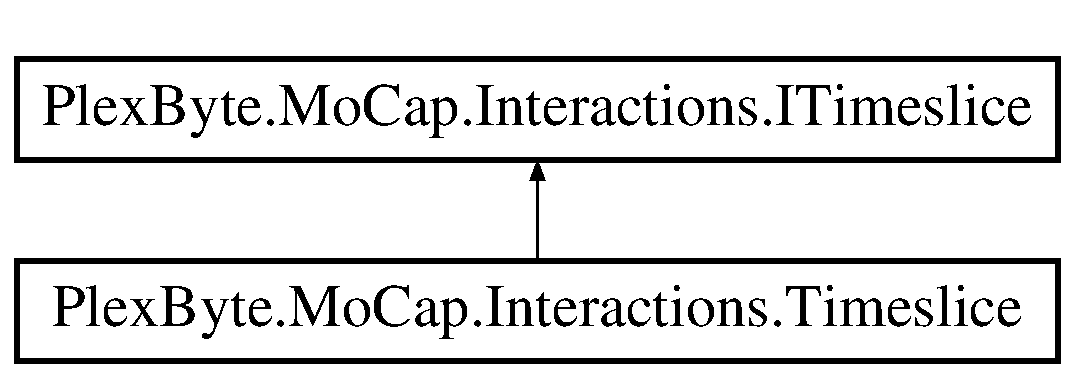
\includegraphics[height=2.000000cm]{class_plex_byte_1_1_mo_cap_1_1_interactions_1_1_timeslice}
\end{center}
\end{figure}
\subsection*{Public Member Functions}
\begin{DoxyCompactItemize}
\item 
\hyperlink{class_plex_byte_1_1_mo_cap_1_1_interactions_1_1_timeslice_ad175821da92a167c2aa6beb22e43b9bd}{Timeslice} (string p\+Id, I\+User p\+User, int p\+Duration, \hyperlink{interface_plex_byte_1_1_mo_cap_1_1_interactions_1_1_i_interaction}{I\+Interaction} p\+Target)
\begin{DoxyCompactList}\small\item\em Constructor of the class \end{DoxyCompactList}\item 
\hyperlink{class_plex_byte_1_1_mo_cap_1_1_interactions_1_1_timeslice_a2a40266754a890b0a0ab13c0a1908b0d}{Timeslice} (string p\+Id, I\+User p\+User, Date\+Time p\+Start\+DT, Date\+Time p\+End\+DT, \hyperlink{interface_plex_byte_1_1_mo_cap_1_1_interactions_1_1_i_interaction}{I\+Interaction} p\+Target)
\begin{DoxyCompactList}\small\item\em Constructor of the class \end{DoxyCompactList}\item 
virtual int \hyperlink{class_plex_byte_1_1_mo_cap_1_1_interactions_1_1_timeslice_acf019f3b3bfe9c64fc32d78e45c41f8a}{Calculate\+Duration} (Date\+Time p\+Start\+DT, Date\+Time p\+End\+DT)
\begin{DoxyCompactList}\small\item\em Calculates the duration between the start and end of a worksession \end{DoxyCompactList}\end{DoxyCompactItemize}
\subsection*{Properties}
\begin{DoxyCompactItemize}
\item 
string \hyperlink{class_plex_byte_1_1_mo_cap_1_1_interactions_1_1_timeslice_ad98eba507161ca5571fdfa56d03c22ab}{Id}\hspace{0.3cm}{\ttfamily  \mbox{[}get\mbox{]}}
\begin{DoxyCompactList}\small\item\em The unique id of the timeslice \end{DoxyCompactList}\item 
int \hyperlink{class_plex_byte_1_1_mo_cap_1_1_interactions_1_1_timeslice_ad5f08401972f9e23eb9afb0ff1ccfbd6}{Duration}\hspace{0.3cm}{\ttfamily  \mbox{[}get\mbox{]}}
\begin{DoxyCompactList}\small\item\em The worktime of the user \end{DoxyCompactList}\item 
string \hyperlink{class_plex_byte_1_1_mo_cap_1_1_interactions_1_1_timeslice_a27e3e7780a2a7fcb05d20418785d16a5}{Description}\hspace{0.3cm}{\ttfamily  \mbox{[}get, set\mbox{]}}
\begin{DoxyCompactList}\small\item\em The description for this timeslice \end{DoxyCompactList}\item 
I\+User \hyperlink{class_plex_byte_1_1_mo_cap_1_1_interactions_1_1_timeslice_aa4ece3cd52590ebbf1c8b27756994a9d}{User}\hspace{0.3cm}{\ttfamily  \mbox{[}get\mbox{]}}
\begin{DoxyCompactList}\small\item\em Owner of the time in the timeslice \end{DoxyCompactList}\item 
\hyperlink{interface_plex_byte_1_1_mo_cap_1_1_interactions_1_1_i_interaction}{I\+Interaction} \hyperlink{class_plex_byte_1_1_mo_cap_1_1_interactions_1_1_timeslice_a80b536958a41037922f51026651aafed}{Target}\hspace{0.3cm}{\ttfamily  \mbox{[}get\mbox{]}}
\begin{DoxyCompactList}\small\item\em The target to which a timeslice is connected \end{DoxyCompactList}\item 
Date\+Time \hyperlink{class_plex_byte_1_1_mo_cap_1_1_interactions_1_1_timeslice_a89403bba6198efa97b362901d8717222}{Created\+Date\+Time}\hspace{0.3cm}{\ttfamily  \mbox{[}get, set\mbox{]}}
\begin{DoxyCompactList}\small\item\em The date and time this timeslice was created \end{DoxyCompactList}\item 
Date\+Time \hyperlink{class_plex_byte_1_1_mo_cap_1_1_interactions_1_1_timeslice_a3fdb3920a4c5148c09fb74ba0d2a5d58}{Modified\+Date\+Time}\hspace{0.3cm}{\ttfamily  \mbox{[}get, set\mbox{]}}
\begin{DoxyCompactList}\small\item\em The date and time this timeslice was modified \end{DoxyCompactList}\end{DoxyCompactItemize}


\subsection{Detailed Description}


Definition at line 10 of file Timeslice.\+cs.



\subsection{Constructor \& Destructor Documentation}
\index{Plex\+Byte\+::\+Mo\+Cap\+::\+Interactions\+::\+Timeslice@{Plex\+Byte\+::\+Mo\+Cap\+::\+Interactions\+::\+Timeslice}!Timeslice@{Timeslice}}
\index{Timeslice@{Timeslice}!Plex\+Byte\+::\+Mo\+Cap\+::\+Interactions\+::\+Timeslice@{Plex\+Byte\+::\+Mo\+Cap\+::\+Interactions\+::\+Timeslice}}
\subsubsection[{\texorpdfstring{Timeslice(string p\+Id, I\+User p\+User, int p\+Duration, I\+Interaction p\+Target)}{Timeslice(string pId, IUser pUser, int pDuration, IInteraction pTarget)}}]{\setlength{\rightskip}{0pt plus 5cm}Plex\+Byte.\+Mo\+Cap.\+Interactions.\+Timeslice.\+Timeslice (
\begin{DoxyParamCaption}
\item[{string}]{p\+Id, }
\item[{I\+User}]{p\+User, }
\item[{int}]{p\+Duration, }
\item[{{\bf I\+Interaction}}]{p\+Target}
\end{DoxyParamCaption}
)}\hypertarget{class_plex_byte_1_1_mo_cap_1_1_interactions_1_1_timeslice_ad175821da92a167c2aa6beb22e43b9bd}{}\label{class_plex_byte_1_1_mo_cap_1_1_interactions_1_1_timeslice_ad175821da92a167c2aa6beb22e43b9bd}


Constructor of the class 


\begin{DoxyParams}{Parameters}
{\em p\+Id} & \\
\hline
{\em p\+User} & \\
\hline
{\em p\+Duration} & \\
\hline
\end{DoxyParams}


Definition at line 53 of file Timeslice.\+cs.

\index{Plex\+Byte\+::\+Mo\+Cap\+::\+Interactions\+::\+Timeslice@{Plex\+Byte\+::\+Mo\+Cap\+::\+Interactions\+::\+Timeslice}!Timeslice@{Timeslice}}
\index{Timeslice@{Timeslice}!Plex\+Byte\+::\+Mo\+Cap\+::\+Interactions\+::\+Timeslice@{Plex\+Byte\+::\+Mo\+Cap\+::\+Interactions\+::\+Timeslice}}
\subsubsection[{\texorpdfstring{Timeslice(string p\+Id, I\+User p\+User, Date\+Time p\+Start\+D\+T, Date\+Time p\+End\+D\+T, I\+Interaction p\+Target)}{Timeslice(string pId, IUser pUser, DateTime pStartDT, DateTime pEndDT, IInteraction pTarget)}}]{\setlength{\rightskip}{0pt plus 5cm}Plex\+Byte.\+Mo\+Cap.\+Interactions.\+Timeslice.\+Timeslice (
\begin{DoxyParamCaption}
\item[{string}]{p\+Id, }
\item[{I\+User}]{p\+User, }
\item[{Date\+Time}]{p\+Start\+DT, }
\item[{Date\+Time}]{p\+End\+DT, }
\item[{{\bf I\+Interaction}}]{p\+Target}
\end{DoxyParamCaption}
)}\hypertarget{class_plex_byte_1_1_mo_cap_1_1_interactions_1_1_timeslice_a2a40266754a890b0a0ab13c0a1908b0d}{}\label{class_plex_byte_1_1_mo_cap_1_1_interactions_1_1_timeslice_a2a40266754a890b0a0ab13c0a1908b0d}


Constructor of the class 


\begin{DoxyParams}{Parameters}
{\em p\+Id} & \\
\hline
{\em p\+User} & \\
\hline
{\em p\+Start\+DT} & \\
\hline
{\em p\+End\+DT} & \\
\hline
\end{DoxyParams}


Definition at line 65 of file Timeslice.\+cs.



\subsection{Member Function Documentation}
\index{Plex\+Byte\+::\+Mo\+Cap\+::\+Interactions\+::\+Timeslice@{Plex\+Byte\+::\+Mo\+Cap\+::\+Interactions\+::\+Timeslice}!Calculate\+Duration@{Calculate\+Duration}}
\index{Calculate\+Duration@{Calculate\+Duration}!Plex\+Byte\+::\+Mo\+Cap\+::\+Interactions\+::\+Timeslice@{Plex\+Byte\+::\+Mo\+Cap\+::\+Interactions\+::\+Timeslice}}
\subsubsection[{\texorpdfstring{Calculate\+Duration(\+Date\+Time p\+Start\+D\+T, Date\+Time p\+End\+D\+T)}{CalculateDuration(DateTime pStartDT, DateTime pEndDT)}}]{\setlength{\rightskip}{0pt plus 5cm}virtual int Plex\+Byte.\+Mo\+Cap.\+Interactions.\+Timeslice.\+Calculate\+Duration (
\begin{DoxyParamCaption}
\item[{Date\+Time}]{p\+Start\+DT, }
\item[{Date\+Time}]{p\+End\+DT}
\end{DoxyParamCaption}
)\hspace{0.3cm}{\ttfamily [virtual]}}\hypertarget{class_plex_byte_1_1_mo_cap_1_1_interactions_1_1_timeslice_acf019f3b3bfe9c64fc32d78e45c41f8a}{}\label{class_plex_byte_1_1_mo_cap_1_1_interactions_1_1_timeslice_acf019f3b3bfe9c64fc32d78e45c41f8a}


Calculates the duration between the start and end of a worksession 


\begin{DoxyParams}{Parameters}
{\em p\+Start\+DT} & \\
\hline
{\em p\+End\+DT} & \\
\hline
\end{DoxyParams}
\begin{DoxyReturn}{Returns}
int duration in Minutes
\end{DoxyReturn}


Implements \hyperlink{interface_plex_byte_1_1_mo_cap_1_1_interactions_1_1_i_timeslice_a4cf2fbe8712024476536bd187dab494c}{Plex\+Byte.\+Mo\+Cap.\+Interactions.\+I\+Timeslice}.



Definition at line 81 of file Timeslice.\+cs.



\subsection{Property Documentation}
\index{Plex\+Byte\+::\+Mo\+Cap\+::\+Interactions\+::\+Timeslice@{Plex\+Byte\+::\+Mo\+Cap\+::\+Interactions\+::\+Timeslice}!Created\+Date\+Time@{Created\+Date\+Time}}
\index{Created\+Date\+Time@{Created\+Date\+Time}!Plex\+Byte\+::\+Mo\+Cap\+::\+Interactions\+::\+Timeslice@{Plex\+Byte\+::\+Mo\+Cap\+::\+Interactions\+::\+Timeslice}}
\subsubsection[{\texorpdfstring{Created\+Date\+Time}{CreatedDateTime}}]{\setlength{\rightskip}{0pt plus 5cm}Date\+Time Plex\+Byte.\+Mo\+Cap.\+Interactions.\+Timeslice.\+Created\+Date\+Time\hspace{0.3cm}{\ttfamily [get]}, {\ttfamily [set]}}\hypertarget{class_plex_byte_1_1_mo_cap_1_1_interactions_1_1_timeslice_a89403bba6198efa97b362901d8717222}{}\label{class_plex_byte_1_1_mo_cap_1_1_interactions_1_1_timeslice_a89403bba6198efa97b362901d8717222}


The date and time this timeslice was created 



Definition at line 37 of file Timeslice.\+cs.

\index{Plex\+Byte\+::\+Mo\+Cap\+::\+Interactions\+::\+Timeslice@{Plex\+Byte\+::\+Mo\+Cap\+::\+Interactions\+::\+Timeslice}!Description@{Description}}
\index{Description@{Description}!Plex\+Byte\+::\+Mo\+Cap\+::\+Interactions\+::\+Timeslice@{Plex\+Byte\+::\+Mo\+Cap\+::\+Interactions\+::\+Timeslice}}
\subsubsection[{\texorpdfstring{Description}{Description}}]{\setlength{\rightskip}{0pt plus 5cm}string Plex\+Byte.\+Mo\+Cap.\+Interactions.\+Timeslice.\+Description\hspace{0.3cm}{\ttfamily [get]}, {\ttfamily [set]}}\hypertarget{class_plex_byte_1_1_mo_cap_1_1_interactions_1_1_timeslice_a27e3e7780a2a7fcb05d20418785d16a5}{}\label{class_plex_byte_1_1_mo_cap_1_1_interactions_1_1_timeslice_a27e3e7780a2a7fcb05d20418785d16a5}


The description for this timeslice 



Definition at line 25 of file Timeslice.\+cs.

\index{Plex\+Byte\+::\+Mo\+Cap\+::\+Interactions\+::\+Timeslice@{Plex\+Byte\+::\+Mo\+Cap\+::\+Interactions\+::\+Timeslice}!Duration@{Duration}}
\index{Duration@{Duration}!Plex\+Byte\+::\+Mo\+Cap\+::\+Interactions\+::\+Timeslice@{Plex\+Byte\+::\+Mo\+Cap\+::\+Interactions\+::\+Timeslice}}
\subsubsection[{\texorpdfstring{Duration}{Duration}}]{\setlength{\rightskip}{0pt plus 5cm}int Plex\+Byte.\+Mo\+Cap.\+Interactions.\+Timeslice.\+Duration\hspace{0.3cm}{\ttfamily [get]}}\hypertarget{class_plex_byte_1_1_mo_cap_1_1_interactions_1_1_timeslice_ad5f08401972f9e23eb9afb0ff1ccfbd6}{}\label{class_plex_byte_1_1_mo_cap_1_1_interactions_1_1_timeslice_ad5f08401972f9e23eb9afb0ff1ccfbd6}


The worktime of the user 



Definition at line 21 of file Timeslice.\+cs.

\index{Plex\+Byte\+::\+Mo\+Cap\+::\+Interactions\+::\+Timeslice@{Plex\+Byte\+::\+Mo\+Cap\+::\+Interactions\+::\+Timeslice}!Id@{Id}}
\index{Id@{Id}!Plex\+Byte\+::\+Mo\+Cap\+::\+Interactions\+::\+Timeslice@{Plex\+Byte\+::\+Mo\+Cap\+::\+Interactions\+::\+Timeslice}}
\subsubsection[{\texorpdfstring{Id}{Id}}]{\setlength{\rightskip}{0pt plus 5cm}string Plex\+Byte.\+Mo\+Cap.\+Interactions.\+Timeslice.\+Id\hspace{0.3cm}{\ttfamily [get]}}\hypertarget{class_plex_byte_1_1_mo_cap_1_1_interactions_1_1_timeslice_ad98eba507161ca5571fdfa56d03c22ab}{}\label{class_plex_byte_1_1_mo_cap_1_1_interactions_1_1_timeslice_ad98eba507161ca5571fdfa56d03c22ab}


The unique id of the timeslice 



Definition at line 17 of file Timeslice.\+cs.

\index{Plex\+Byte\+::\+Mo\+Cap\+::\+Interactions\+::\+Timeslice@{Plex\+Byte\+::\+Mo\+Cap\+::\+Interactions\+::\+Timeslice}!Modified\+Date\+Time@{Modified\+Date\+Time}}
\index{Modified\+Date\+Time@{Modified\+Date\+Time}!Plex\+Byte\+::\+Mo\+Cap\+::\+Interactions\+::\+Timeslice@{Plex\+Byte\+::\+Mo\+Cap\+::\+Interactions\+::\+Timeslice}}
\subsubsection[{\texorpdfstring{Modified\+Date\+Time}{ModifiedDateTime}}]{\setlength{\rightskip}{0pt plus 5cm}Date\+Time Plex\+Byte.\+Mo\+Cap.\+Interactions.\+Timeslice.\+Modified\+Date\+Time\hspace{0.3cm}{\ttfamily [get]}, {\ttfamily [set]}}\hypertarget{class_plex_byte_1_1_mo_cap_1_1_interactions_1_1_timeslice_a3fdb3920a4c5148c09fb74ba0d2a5d58}{}\label{class_plex_byte_1_1_mo_cap_1_1_interactions_1_1_timeslice_a3fdb3920a4c5148c09fb74ba0d2a5d58}


The date and time this timeslice was modified 



Definition at line 41 of file Timeslice.\+cs.

\index{Plex\+Byte\+::\+Mo\+Cap\+::\+Interactions\+::\+Timeslice@{Plex\+Byte\+::\+Mo\+Cap\+::\+Interactions\+::\+Timeslice}!Target@{Target}}
\index{Target@{Target}!Plex\+Byte\+::\+Mo\+Cap\+::\+Interactions\+::\+Timeslice@{Plex\+Byte\+::\+Mo\+Cap\+::\+Interactions\+::\+Timeslice}}
\subsubsection[{\texorpdfstring{Target}{Target}}]{\setlength{\rightskip}{0pt plus 5cm}{\bf I\+Interaction} Plex\+Byte.\+Mo\+Cap.\+Interactions.\+Timeslice.\+Target\hspace{0.3cm}{\ttfamily [get]}}\hypertarget{class_plex_byte_1_1_mo_cap_1_1_interactions_1_1_timeslice_a80b536958a41037922f51026651aafed}{}\label{class_plex_byte_1_1_mo_cap_1_1_interactions_1_1_timeslice_a80b536958a41037922f51026651aafed}


The target to which a timeslice is connected 



Definition at line 33 of file Timeslice.\+cs.

\index{Plex\+Byte\+::\+Mo\+Cap\+::\+Interactions\+::\+Timeslice@{Plex\+Byte\+::\+Mo\+Cap\+::\+Interactions\+::\+Timeslice}!User@{User}}
\index{User@{User}!Plex\+Byte\+::\+Mo\+Cap\+::\+Interactions\+::\+Timeslice@{Plex\+Byte\+::\+Mo\+Cap\+::\+Interactions\+::\+Timeslice}}
\subsubsection[{\texorpdfstring{User}{User}}]{\setlength{\rightskip}{0pt plus 5cm}I\+User Plex\+Byte.\+Mo\+Cap.\+Interactions.\+Timeslice.\+User\hspace{0.3cm}{\ttfamily [get]}}\hypertarget{class_plex_byte_1_1_mo_cap_1_1_interactions_1_1_timeslice_aa4ece3cd52590ebbf1c8b27756994a9d}{}\label{class_plex_byte_1_1_mo_cap_1_1_interactions_1_1_timeslice_aa4ece3cd52590ebbf1c8b27756994a9d}


Owner of the time in the timeslice 



Definition at line 29 of file Timeslice.\+cs.



The documentation for this class was generated from the following file\+:\begin{DoxyCompactItemize}
\item 
D\+:/\+Users/\+Christian\+B/\+Documents/\+\_\+\+H\+F Infomatik/\+Git\+Hub\+\_\+\+Repos/\+Mo\+Cap/\+Plex\+Byte.\+Mo\+Cap/\+Plex\+Byte.\+Mo\+Cap.\+Interactions/\hyperlink{_timeslice_8cs}{Timeslice.\+cs}\end{DoxyCompactItemize}

\hypertarget{class_plex_byte_1_1_mo_cap_1_1_interactions_1_1_vote}{}\section{Plex\+Byte.\+Mo\+Cap.\+Interactions.\+Vote Class Reference}
\label{class_plex_byte_1_1_mo_cap_1_1_interactions_1_1_vote}\index{Plex\+Byte.\+Mo\+Cap.\+Interactions.\+Vote@{Plex\+Byte.\+Mo\+Cap.\+Interactions.\+Vote}}


This class holds information about a users choice, containing the user and his choice selected  


Inheritance diagram for Plex\+Byte.\+Mo\+Cap.\+Interactions.\+Vote\+:\begin{figure}[H]
\begin{center}
\leavevmode
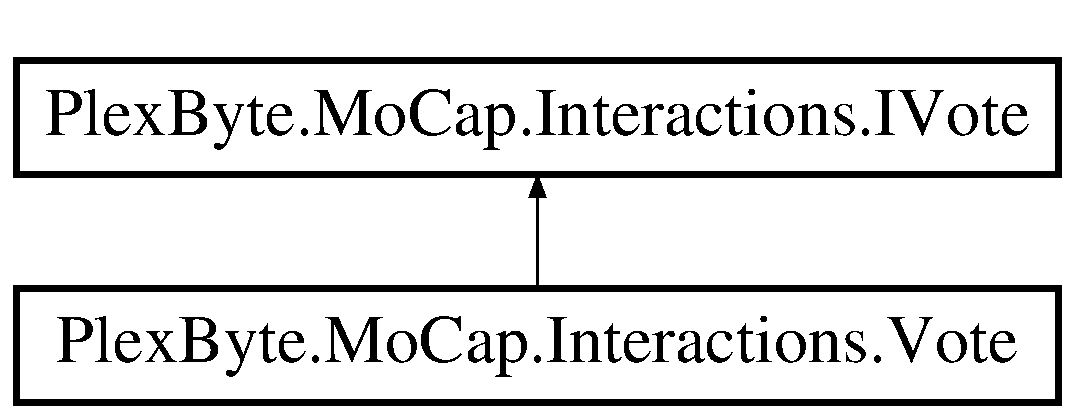
\includegraphics[height=2.000000cm]{class_plex_byte_1_1_mo_cap_1_1_interactions_1_1_vote}
\end{center}
\end{figure}
\subsection*{Public Member Functions}
\begin{DoxyCompactItemize}
\item 
\hyperlink{class_plex_byte_1_1_mo_cap_1_1_interactions_1_1_vote_a23a08f2604526ff8f6dbb330e09829f9}{Vote} (string p\+Id, I\+User p\+User, \hyperlink{interface_plex_byte_1_1_mo_cap_1_1_interactions_1_1_i_survey_option}{I\+Survey\+Option} p\+Option)
\begin{DoxyCompactList}\small\item\em The constructor of the class \end{DoxyCompactList}\end{DoxyCompactItemize}
\subsection*{Properties}
\begin{DoxyCompactItemize}
\item 
Date\+Time \hyperlink{class_plex_byte_1_1_mo_cap_1_1_interactions_1_1_vote_ae7cb6cc9d86a52d927f689c926a7e8a4}{Created\+Date\+Time}\hspace{0.3cm}{\ttfamily  \mbox{[}get\mbox{]}}
\begin{DoxyCompactList}\small\item\em The date and time this vote was left \end{DoxyCompactList}\item 
string \hyperlink{class_plex_byte_1_1_mo_cap_1_1_interactions_1_1_vote_a9ee8f835267b3c453ca79564e11a365f}{Id}\hspace{0.3cm}{\ttfamily  \mbox{[}get\mbox{]}}
\begin{DoxyCompactList}\small\item\em The unique id of this object \end{DoxyCompactList}\item 
\hyperlink{interface_plex_byte_1_1_mo_cap_1_1_interactions_1_1_i_survey_option}{I\+Survey\+Option} \hyperlink{class_plex_byte_1_1_mo_cap_1_1_interactions_1_1_vote_a84ca623bee92a24c658a532234f06a8f}{Option}\hspace{0.3cm}{\ttfamily  \mbox{[}get\mbox{]}}
\begin{DoxyCompactList}\small\item\em The survey option chosen by the user \end{DoxyCompactList}\item 
I\+User \hyperlink{class_plex_byte_1_1_mo_cap_1_1_interactions_1_1_vote_a704a068395851baacc22e71db46d3ea8}{User}\hspace{0.3cm}{\ttfamily  \mbox{[}get\mbox{]}}
\begin{DoxyCompactList}\small\item\em The user who votes \end{DoxyCompactList}\end{DoxyCompactItemize}


\subsection{Detailed Description}
This class holds information about a users choice, containing the user and his choice selected 



Definition at line 13 of file Vote.\+cs.



\subsection{Constructor \& Destructor Documentation}
\index{Plex\+Byte\+::\+Mo\+Cap\+::\+Interactions\+::\+Vote@{Plex\+Byte\+::\+Mo\+Cap\+::\+Interactions\+::\+Vote}!Vote@{Vote}}
\index{Vote@{Vote}!Plex\+Byte\+::\+Mo\+Cap\+::\+Interactions\+::\+Vote@{Plex\+Byte\+::\+Mo\+Cap\+::\+Interactions\+::\+Vote}}
\subsubsection[{\texorpdfstring{Vote(string p\+Id, I\+User p\+User, I\+Survey\+Option p\+Option)}{Vote(string pId, IUser pUser, ISurveyOption pOption)}}]{\setlength{\rightskip}{0pt plus 5cm}Plex\+Byte.\+Mo\+Cap.\+Interactions.\+Vote.\+Vote (
\begin{DoxyParamCaption}
\item[{string}]{p\+Id, }
\item[{I\+User}]{p\+User, }
\item[{{\bf I\+Survey\+Option}}]{p\+Option}
\end{DoxyParamCaption}
)}\hypertarget{class_plex_byte_1_1_mo_cap_1_1_interactions_1_1_vote_a23a08f2604526ff8f6dbb330e09829f9}{}\label{class_plex_byte_1_1_mo_cap_1_1_interactions_1_1_vote_a23a08f2604526ff8f6dbb330e09829f9}


The constructor of the class 


\begin{DoxyParams}{Parameters}
{\em p\+Id} & The unique id of this object\\
\hline
{\em p\+User} & The user who made the choice\\
\hline
{\em p\+Option} & The choice that was selected\\
\hline
\end{DoxyParams}


Definition at line 21 of file Vote.\+cs.



\subsection{Property Documentation}
\index{Plex\+Byte\+::\+Mo\+Cap\+::\+Interactions\+::\+Vote@{Plex\+Byte\+::\+Mo\+Cap\+::\+Interactions\+::\+Vote}!Created\+Date\+Time@{Created\+Date\+Time}}
\index{Created\+Date\+Time@{Created\+Date\+Time}!Plex\+Byte\+::\+Mo\+Cap\+::\+Interactions\+::\+Vote@{Plex\+Byte\+::\+Mo\+Cap\+::\+Interactions\+::\+Vote}}
\subsubsection[{\texorpdfstring{Created\+Date\+Time}{CreatedDateTime}}]{\setlength{\rightskip}{0pt plus 5cm}Date\+Time Plex\+Byte.\+Mo\+Cap.\+Interactions.\+Vote.\+Created\+Date\+Time\hspace{0.3cm}{\ttfamily [get]}}\hypertarget{class_plex_byte_1_1_mo_cap_1_1_interactions_1_1_vote_ae7cb6cc9d86a52d927f689c926a7e8a4}{}\label{class_plex_byte_1_1_mo_cap_1_1_interactions_1_1_vote_ae7cb6cc9d86a52d927f689c926a7e8a4}


The date and time this vote was left 



Definition at line 31 of file Vote.\+cs.

\index{Plex\+Byte\+::\+Mo\+Cap\+::\+Interactions\+::\+Vote@{Plex\+Byte\+::\+Mo\+Cap\+::\+Interactions\+::\+Vote}!Id@{Id}}
\index{Id@{Id}!Plex\+Byte\+::\+Mo\+Cap\+::\+Interactions\+::\+Vote@{Plex\+Byte\+::\+Mo\+Cap\+::\+Interactions\+::\+Vote}}
\subsubsection[{\texorpdfstring{Id}{Id}}]{\setlength{\rightskip}{0pt plus 5cm}string Plex\+Byte.\+Mo\+Cap.\+Interactions.\+Vote.\+Id\hspace{0.3cm}{\ttfamily [get]}}\hypertarget{class_plex_byte_1_1_mo_cap_1_1_interactions_1_1_vote_a9ee8f835267b3c453ca79564e11a365f}{}\label{class_plex_byte_1_1_mo_cap_1_1_interactions_1_1_vote_a9ee8f835267b3c453ca79564e11a365f}


The unique id of this object 



Definition at line 36 of file Vote.\+cs.

\index{Plex\+Byte\+::\+Mo\+Cap\+::\+Interactions\+::\+Vote@{Plex\+Byte\+::\+Mo\+Cap\+::\+Interactions\+::\+Vote}!Option@{Option}}
\index{Option@{Option}!Plex\+Byte\+::\+Mo\+Cap\+::\+Interactions\+::\+Vote@{Plex\+Byte\+::\+Mo\+Cap\+::\+Interactions\+::\+Vote}}
\subsubsection[{\texorpdfstring{Option}{Option}}]{\setlength{\rightskip}{0pt plus 5cm}{\bf I\+Survey\+Option} Plex\+Byte.\+Mo\+Cap.\+Interactions.\+Vote.\+Option\hspace{0.3cm}{\ttfamily [get]}}\hypertarget{class_plex_byte_1_1_mo_cap_1_1_interactions_1_1_vote_a84ca623bee92a24c658a532234f06a8f}{}\label{class_plex_byte_1_1_mo_cap_1_1_interactions_1_1_vote_a84ca623bee92a24c658a532234f06a8f}


The survey option chosen by the user 



Definition at line 41 of file Vote.\+cs.

\index{Plex\+Byte\+::\+Mo\+Cap\+::\+Interactions\+::\+Vote@{Plex\+Byte\+::\+Mo\+Cap\+::\+Interactions\+::\+Vote}!User@{User}}
\index{User@{User}!Plex\+Byte\+::\+Mo\+Cap\+::\+Interactions\+::\+Vote@{Plex\+Byte\+::\+Mo\+Cap\+::\+Interactions\+::\+Vote}}
\subsubsection[{\texorpdfstring{User}{User}}]{\setlength{\rightskip}{0pt plus 5cm}I\+User Plex\+Byte.\+Mo\+Cap.\+Interactions.\+Vote.\+User\hspace{0.3cm}{\ttfamily [get]}}\hypertarget{class_plex_byte_1_1_mo_cap_1_1_interactions_1_1_vote_a704a068395851baacc22e71db46d3ea8}{}\label{class_plex_byte_1_1_mo_cap_1_1_interactions_1_1_vote_a704a068395851baacc22e71db46d3ea8}


The user who votes 



Definition at line 46 of file Vote.\+cs.



The documentation for this class was generated from the following file\+:\begin{DoxyCompactItemize}
\item 
D\+:/\+Users/\+Christian\+B/\+Documents/\+\_\+\+H\+F Infomatik/\+Git\+Hub\+\_\+\+Repos/\+Mo\+Cap/\+Plex\+Byte.\+Mo\+Cap/\+Plex\+Byte.\+Mo\+Cap.\+Interactions/\hyperlink{_vote_8cs}{Vote.\+cs}\end{DoxyCompactItemize}

\chapter{File Documentation}
\hypertarget{_account_8cs}{}\section{D\+:/\+Users/\+Christian\+B/\+Documents/\+\_\+\+HF Infomatik/\+Git\+Hub\+\_\+\+Repos/\+Mo\+Cap/\+Plex\+Byte.Mo\+Cap/\+Plex\+Byte.Mo\+Cap.\+Interactions/\+Account.cs File Reference}
\label{_account_8cs}\index{D\+:/\+Users/\+Christian\+B/\+Documents/\+\_\+\+H\+F Infomatik/\+Git\+Hub\+\_\+\+Repos/\+Mo\+Cap/\+Plex\+Byte.\+Mo\+Cap/\+Plex\+Byte.\+Mo\+Cap.\+Interactions/\+Account.\+cs@{D\+:/\+Users/\+Christian\+B/\+Documents/\+\_\+\+H\+F Infomatik/\+Git\+Hub\+\_\+\+Repos/\+Mo\+Cap/\+Plex\+Byte.\+Mo\+Cap/\+Plex\+Byte.\+Mo\+Cap.\+Interactions/\+Account.\+cs}}
\subsection*{Classes}
\begin{DoxyCompactItemize}
\item 
class \hyperlink{class_plex_byte_1_1_mo_cap_1_1_interactions_1_1_account}{Plex\+Byte.\+Mo\+Cap.\+Interactions.\+Account}
\end{DoxyCompactItemize}
\subsection*{Namespaces}
\begin{DoxyCompactItemize}
\item 
namespace \hyperlink{namespace_plex_byte_1_1_mo_cap_1_1_interactions}{Plex\+Byte.\+Mo\+Cap.\+Interactions}
\end{DoxyCompactItemize}

\hypertarget{_expense_8cs}{}\section{D\+:/\+Users/\+Christian\+B/\+Documents/\+\_\+\+HF Infomatik/\+Git\+Hub\+\_\+\+Repos/\+Mo\+Cap/\+Plex\+Byte.Mo\+Cap/\+Plex\+Byte.Mo\+Cap.\+Interactions/\+Expense.cs File Reference}
\label{_expense_8cs}\index{D\+:/\+Users/\+Christian\+B/\+Documents/\+\_\+\+H\+F Infomatik/\+Git\+Hub\+\_\+\+Repos/\+Mo\+Cap/\+Plex\+Byte.\+Mo\+Cap/\+Plex\+Byte.\+Mo\+Cap.\+Interactions/\+Expense.\+cs@{D\+:/\+Users/\+Christian\+B/\+Documents/\+\_\+\+H\+F Infomatik/\+Git\+Hub\+\_\+\+Repos/\+Mo\+Cap/\+Plex\+Byte.\+Mo\+Cap/\+Plex\+Byte.\+Mo\+Cap.\+Interactions/\+Expense.\+cs}}
\subsection*{Classes}
\begin{DoxyCompactItemize}
\item 
class \hyperlink{class_plex_byte_1_1_mo_cap_1_1_interactions_1_1_expense}{Plex\+Byte.\+Mo\+Cap.\+Interactions.\+Expense}
\end{DoxyCompactItemize}
\subsection*{Namespaces}
\begin{DoxyCompactItemize}
\item 
namespace \hyperlink{namespace_plex_byte_1_1_mo_cap_1_1_interactions}{Plex\+Byte.\+Mo\+Cap.\+Interactions}
\end{DoxyCompactItemize}

\hypertarget{_i_account_8cs}{}\section{D\+:/\+Users/\+Christian\+B/\+Documents/\+\_\+\+HF Infomatik/\+Git\+Hub\+\_\+\+Repos/\+Mo\+Cap/\+Plex\+Byte.Mo\+Cap/\+Plex\+Byte.Mo\+Cap.\+Interactions/\+I\+Account.cs File Reference}
\label{_i_account_8cs}\index{D\+:/\+Users/\+Christian\+B/\+Documents/\+\_\+\+H\+F Infomatik/\+Git\+Hub\+\_\+\+Repos/\+Mo\+Cap/\+Plex\+Byte.\+Mo\+Cap/\+Plex\+Byte.\+Mo\+Cap.\+Interactions/\+I\+Account.\+cs@{D\+:/\+Users/\+Christian\+B/\+Documents/\+\_\+\+H\+F Infomatik/\+Git\+Hub\+\_\+\+Repos/\+Mo\+Cap/\+Plex\+Byte.\+Mo\+Cap/\+Plex\+Byte.\+Mo\+Cap.\+Interactions/\+I\+Account.\+cs}}
\subsection*{Classes}
\begin{DoxyCompactItemize}
\item 
interface \hyperlink{interface_plex_byte_1_1_mo_cap_1_1_interactions_1_1_i_account}{Plex\+Byte.\+Mo\+Cap.\+Interactions.\+I\+Account}
\end{DoxyCompactItemize}
\subsection*{Namespaces}
\begin{DoxyCompactItemize}
\item 
namespace \hyperlink{namespace_plex_byte_1_1_mo_cap_1_1_interactions}{Plex\+Byte.\+Mo\+Cap.\+Interactions}
\end{DoxyCompactItemize}
\subsection*{Functions}
\begin{DoxyCompactItemize}
\item 
delegate void \hyperlink{namespace_plex_byte_1_1_mo_cap_1_1_interactions_a7c03c08c6f524b34193985c455985f1f}{Plex\+Byte.\+Mo\+Cap.\+Interactions.\+Expense\+Add} (object sender, Interaction\+Event\+Args e)
\item 
delegate void \hyperlink{namespace_plex_byte_1_1_mo_cap_1_1_interactions_a600557b92ababd90f6a91c524998565a}{Plex\+Byte.\+Mo\+Cap.\+Interactions.\+Timeslice\+Add} (object sender, Interaction\+Event\+Args e)
\end{DoxyCompactItemize}

\hypertarget{_i_expense_8cs}{}\section{D\+:/\+Users/\+Christian\+B/\+Documents/\+\_\+\+HF Infomatik/\+Git\+Hub\+\_\+\+Repos/\+Mo\+Cap/\+Plex\+Byte.Mo\+Cap/\+Plex\+Byte.Mo\+Cap.\+Interactions/\+I\+Expense.cs File Reference}
\label{_i_expense_8cs}\index{D\+:/\+Users/\+Christian\+B/\+Documents/\+\_\+\+H\+F Infomatik/\+Git\+Hub\+\_\+\+Repos/\+Mo\+Cap/\+Plex\+Byte.\+Mo\+Cap/\+Plex\+Byte.\+Mo\+Cap.\+Interactions/\+I\+Expense.\+cs@{D\+:/\+Users/\+Christian\+B/\+Documents/\+\_\+\+H\+F Infomatik/\+Git\+Hub\+\_\+\+Repos/\+Mo\+Cap/\+Plex\+Byte.\+Mo\+Cap/\+Plex\+Byte.\+Mo\+Cap.\+Interactions/\+I\+Expense.\+cs}}
\subsection*{Classes}
\begin{DoxyCompactItemize}
\item 
interface \hyperlink{interface_plex_byte_1_1_mo_cap_1_1_interactions_1_1_i_expense}{Plex\+Byte.\+Mo\+Cap.\+Interactions.\+I\+Expense}
\end{DoxyCompactItemize}
\subsection*{Namespaces}
\begin{DoxyCompactItemize}
\item 
namespace \hyperlink{namespace_plex_byte_1_1_mo_cap_1_1_interactions}{Plex\+Byte.\+Mo\+Cap.\+Interactions}
\end{DoxyCompactItemize}

\hypertarget{_i_interaction_8cs}{}\section{D\+:/\+Users/\+Christian\+B/\+Documents/\+\_\+\+HF Infomatik/\+Git\+Hub\+\_\+\+Repos/\+Mo\+Cap/\+Plex\+Byte.Mo\+Cap/\+Plex\+Byte.Mo\+Cap.\+Interactions/\+I\+Interaction.cs File Reference}
\label{_i_interaction_8cs}\index{D\+:/\+Users/\+Christian\+B/\+Documents/\+\_\+\+H\+F Infomatik/\+Git\+Hub\+\_\+\+Repos/\+Mo\+Cap/\+Plex\+Byte.\+Mo\+Cap/\+Plex\+Byte.\+Mo\+Cap.\+Interactions/\+I\+Interaction.\+cs@{D\+:/\+Users/\+Christian\+B/\+Documents/\+\_\+\+H\+F Infomatik/\+Git\+Hub\+\_\+\+Repos/\+Mo\+Cap/\+Plex\+Byte.\+Mo\+Cap/\+Plex\+Byte.\+Mo\+Cap.\+Interactions/\+I\+Interaction.\+cs}}
\subsection*{Classes}
\begin{DoxyCompactItemize}
\item 
interface \hyperlink{interface_plex_byte_1_1_mo_cap_1_1_interactions_1_1_i_interaction}{Plex\+Byte.\+Mo\+Cap.\+Interactions.\+I\+Interaction}
\end{DoxyCompactItemize}
\subsection*{Namespaces}
\begin{DoxyCompactItemize}
\item 
namespace \hyperlink{namespace_plex_byte_1_1_mo_cap_1_1_interactions}{Plex\+Byte.\+Mo\+Cap.\+Interactions}
\end{DoxyCompactItemize}
\subsection*{Functions}
\begin{DoxyCompactItemize}
\item 
delegate void \hyperlink{namespace_plex_byte_1_1_mo_cap_1_1_interactions_ac81ac3321ab2b018c75ad2c18ec15b9e}{Plex\+Byte.\+Mo\+Cap.\+Interactions.\+Complete} (object sender, Interaction\+Event\+Args e)
\item 
delegate void \hyperlink{namespace_plex_byte_1_1_mo_cap_1_1_interactions_a490186f613e46adce26244f3b2c78a58}{Plex\+Byte.\+Mo\+Cap.\+Interactions.\+Modify} (object sender, Interaction\+Event\+Args e)
\item 
delegate void \hyperlink{namespace_plex_byte_1_1_mo_cap_1_1_interactions_af2ff213e81451f96fc74bfad114cecde}{Plex\+Byte.\+Mo\+Cap.\+Interactions.\+State\+Change} (object sender, Interaction\+Event\+Args e)
\end{DoxyCompactItemize}

\hypertarget{_i_interaction_factory_8cs}{}\section{D\+:/\+Users/\+Christian\+B/\+Documents/\+\_\+\+HF Infomatik/\+Git\+Hub\+\_\+\+Repos/\+Mo\+Cap/\+Plex\+Byte.Mo\+Cap/\+Plex\+Byte.Mo\+Cap.\+Interactions/\+I\+Interaction\+Factory.cs File Reference}
\label{_i_interaction_factory_8cs}\index{D\+:/\+Users/\+Christian\+B/\+Documents/\+\_\+\+H\+F Infomatik/\+Git\+Hub\+\_\+\+Repos/\+Mo\+Cap/\+Plex\+Byte.\+Mo\+Cap/\+Plex\+Byte.\+Mo\+Cap.\+Interactions/\+I\+Interaction\+Factory.\+cs@{D\+:/\+Users/\+Christian\+B/\+Documents/\+\_\+\+H\+F Infomatik/\+Git\+Hub\+\_\+\+Repos/\+Mo\+Cap/\+Plex\+Byte.\+Mo\+Cap/\+Plex\+Byte.\+Mo\+Cap.\+Interactions/\+I\+Interaction\+Factory.\+cs}}
\subsection*{Classes}
\begin{DoxyCompactItemize}
\item 
interface \hyperlink{interface_plex_byte_1_1_mo_cap_1_1_interactions_1_1_i_interaction_factory}{Plex\+Byte.\+Mo\+Cap.\+Interactions.\+I\+Interaction\+Factory}
\end{DoxyCompactItemize}
\subsection*{Namespaces}
\begin{DoxyCompactItemize}
\item 
namespace \hyperlink{namespace_plex_byte_1_1_mo_cap_1_1_interactions}{Plex\+Byte.\+Mo\+Cap.\+Interactions}
\end{DoxyCompactItemize}

\hypertarget{_interaction_8cs}{}\section{D\+:/\+Users/\+Christian\+B/\+Documents/\+\_\+\+HF Infomatik/\+Git\+Hub\+\_\+\+Repos/\+Mo\+Cap/\+Plex\+Byte.Mo\+Cap/\+Plex\+Byte.Mo\+Cap.\+Interactions/\+Interaction.cs File Reference}
\label{_interaction_8cs}\index{D\+:/\+Users/\+Christian\+B/\+Documents/\+\_\+\+H\+F Infomatik/\+Git\+Hub\+\_\+\+Repos/\+Mo\+Cap/\+Plex\+Byte.\+Mo\+Cap/\+Plex\+Byte.\+Mo\+Cap.\+Interactions/\+Interaction.\+cs@{D\+:/\+Users/\+Christian\+B/\+Documents/\+\_\+\+H\+F Infomatik/\+Git\+Hub\+\_\+\+Repos/\+Mo\+Cap/\+Plex\+Byte.\+Mo\+Cap/\+Plex\+Byte.\+Mo\+Cap.\+Interactions/\+Interaction.\+cs}}
\subsection*{Classes}
\begin{DoxyCompactItemize}
\item 
class \hyperlink{class_plex_byte_1_1_mo_cap_1_1_interactions_1_1_interaction}{Plex\+Byte.\+Mo\+Cap.\+Interactions.\+Interaction}
\end{DoxyCompactItemize}
\subsection*{Namespaces}
\begin{DoxyCompactItemize}
\item 
namespace \hyperlink{namespace_plex_byte_1_1_mo_cap_1_1_interactions}{Plex\+Byte.\+Mo\+Cap.\+Interactions}
\end{DoxyCompactItemize}

\hypertarget{_interaction_attributes_8cs}{}\section{D\+:/\+Users/\+Christian\+B/\+Documents/\+\_\+\+HF Infomatik/\+Git\+Hub\+\_\+\+Repos/\+Mo\+Cap/\+Plex\+Byte.Mo\+Cap/\+Plex\+Byte.Mo\+Cap.\+Interactions/\+Interaction\+Attributes.cs File Reference}
\label{_interaction_attributes_8cs}\index{D\+:/\+Users/\+Christian\+B/\+Documents/\+\_\+\+H\+F Infomatik/\+Git\+Hub\+\_\+\+Repos/\+Mo\+Cap/\+Plex\+Byte.\+Mo\+Cap/\+Plex\+Byte.\+Mo\+Cap.\+Interactions/\+Interaction\+Attributes.\+cs@{D\+:/\+Users/\+Christian\+B/\+Documents/\+\_\+\+H\+F Infomatik/\+Git\+Hub\+\_\+\+Repos/\+Mo\+Cap/\+Plex\+Byte.\+Mo\+Cap/\+Plex\+Byte.\+Mo\+Cap.\+Interactions/\+Interaction\+Attributes.\+cs}}
\subsection*{Namespaces}
\begin{DoxyCompactItemize}
\item 
namespace \hyperlink{namespace_plex_byte_1_1_mo_cap_1_1_interactions}{Plex\+Byte.\+Mo\+Cap.\+Interactions}
\end{DoxyCompactItemize}
\subsection*{Enumerations}
\begin{DoxyCompactItemize}
\item 
enum \hyperlink{namespace_plex_byte_1_1_mo_cap_1_1_interactions_aa78ff2ea1c7ea92537cb6b3552b6a7da}{Plex\+Byte.\+Mo\+Cap.\+Interactions.\+Interaction\+Attributes} \{ \\*
\hyperlink{namespace_plex_byte_1_1_mo_cap_1_1_interactions_aa78ff2ea1c7ea92537cb6b3552b6a7daaa10fd73f3ddd28f1e63ab772e0e204cd}{Plex\+Byte.\+Mo\+Cap.\+Interactions.\+Interaction\+Attributes.\+Created\+Date\+Time}, 
\hyperlink{namespace_plex_byte_1_1_mo_cap_1_1_interactions_aa78ff2ea1c7ea92537cb6b3552b6a7daa88c28c0fe268a710416759f5dffc06be}{Plex\+Byte.\+Mo\+Cap.\+Interactions.\+Interaction\+Attributes.\+End\+Date\+Time}, 
\hyperlink{namespace_plex_byte_1_1_mo_cap_1_1_interactions_aa78ff2ea1c7ea92537cb6b3552b6a7daa186152e397e1f2c77bd57fcb46acedf3}{Plex\+Byte.\+Mo\+Cap.\+Interactions.\+Interaction\+Attributes.\+Start\+Date\+Time}, 
\hyperlink{namespace_plex_byte_1_1_mo_cap_1_1_interactions_aa78ff2ea1c7ea92537cb6b3552b6a7daa0205bd44391ac41fa714e1d718993bbe}{Plex\+Byte.\+Mo\+Cap.\+Interactions.\+Interaction\+Attributes.\+Is\+Active}, 
\\*
\hyperlink{namespace_plex_byte_1_1_mo_cap_1_1_interactions_aa78ff2ea1c7ea92537cb6b3552b6a7daab6f4a2ec6356bbd56d49f2096bf9d3d3}{Plex\+Byte.\+Mo\+Cap.\+Interactions.\+Interaction\+Attributes.\+Owner}, 
\hyperlink{namespace_plex_byte_1_1_mo_cap_1_1_interactions_aa78ff2ea1c7ea92537cb6b3552b6a7daa46a2a41cc6e552044816a2d04634545d}{Plex\+Byte.\+Mo\+Cap.\+Interactions.\+Interaction\+Attributes.\+State}, 
\hyperlink{namespace_plex_byte_1_1_mo_cap_1_1_interactions_aa78ff2ea1c7ea92537cb6b3552b6a7daa9dffbf69ffba8bc38bc4e01abf4b1675}{Plex\+Byte.\+Mo\+Cap.\+Interactions.\+Interaction\+Attributes.\+Text}, 
\hyperlink{namespace_plex_byte_1_1_mo_cap_1_1_interactions_aa78ff2ea1c7ea92537cb6b3552b6a7daaa1fa27779242b4902f7ae3bdd5c6d508}{Plex\+Byte.\+Mo\+Cap.\+Interactions.\+Interaction\+Attributes.\+Type}, 
\\*
\hyperlink{namespace_plex_byte_1_1_mo_cap_1_1_interactions_aa78ff2ea1c7ea92537cb6b3552b6a7daa13bdab490cf0aa0bec1e26512f03f383}{Plex\+Byte.\+Mo\+Cap.\+Interactions.\+Interaction\+Attributes.\+Vote\+List}, 
\hyperlink{namespace_plex_byte_1_1_mo_cap_1_1_interactions_aa78ff2ea1c7ea92537cb6b3552b6a7daa722212420bfcea4162c4c64e339e8e52}{Plex\+Byte.\+Mo\+Cap.\+Interactions.\+Interaction\+Attributes.\+Option\+List}, 
\hyperlink{namespace_plex_byte_1_1_mo_cap_1_1_interactions_aa78ff2ea1c7ea92537cb6b3552b6a7daa02b034071e3c602d1ca1e6762b01fd08}{Plex\+Byte.\+Mo\+Cap.\+Interactions.\+Interaction\+Attributes.\+User\+List}, 
\hyperlink{namespace_plex_byte_1_1_mo_cap_1_1_interactions_aa78ff2ea1c7ea92537cb6b3552b6a7daa46b5f8c58b679b4243cbdb5749642c86}{Plex\+Byte.\+Mo\+Cap.\+Interactions.\+Interaction\+Attributes.\+Progress}, 
\\*
\hyperlink{namespace_plex_byte_1_1_mo_cap_1_1_interactions_aa78ff2ea1c7ea92537cb6b3552b6a7daa822bead6c149ffacbe7a12c44c3958ed}{Plex\+Byte.\+Mo\+Cap.\+Interactions.\+Interaction\+Attributes.\+Budget}, 
\hyperlink{namespace_plex_byte_1_1_mo_cap_1_1_interactions_aa78ff2ea1c7ea92537cb6b3552b6a7daafeadb1427974216b9cce2d063b99f676}{Plex\+Byte.\+Mo\+Cap.\+Interactions.\+Interaction\+Attributes.\+Used\+Budget}, 
\hyperlink{namespace_plex_byte_1_1_mo_cap_1_1_interactions_aa78ff2ea1c7ea92537cb6b3552b6a7daae797bfc09ca332460143a197adc82069}{Plex\+Byte.\+Mo\+Cap.\+Interactions.\+Interaction\+Attributes.\+Used\+Duration}, 
\hyperlink{namespace_plex_byte_1_1_mo_cap_1_1_interactions_aa78ff2ea1c7ea92537cb6b3552b6a7daab3f0f2eb7b25831c4e3f1d6fb7d48130}{Plex\+Byte.\+Mo\+Cap.\+Interactions.\+Interaction\+Attributes.\+Task\+List}, 
\\*
\hyperlink{namespace_plex_byte_1_1_mo_cap_1_1_interactions_aa78ff2ea1c7ea92537cb6b3552b6a7daaf698bdcd42e8985484f12fc4245a4843}{Plex\+Byte.\+Mo\+Cap.\+Interactions.\+Interaction\+Attributes.\+Survey\+List}, 
\hyperlink{namespace_plex_byte_1_1_mo_cap_1_1_interactions_aa78ff2ea1c7ea92537cb6b3552b6a7daa3547319d6f4e11ac104fe2012b8c99c4}{Plex\+Byte.\+Mo\+Cap.\+Interactions.\+Interaction\+Attributes.\+Member\+List}, 
\hyperlink{namespace_plex_byte_1_1_mo_cap_1_1_interactions_aa78ff2ea1c7ea92537cb6b3552b6a7daa1a7f5ee14da52a7231b80e347f1fe0eb}{Plex\+Byte.\+Mo\+Cap.\+Interactions.\+Interaction\+Attributes.\+Invitation\+List}, 
\hyperlink{namespace_plex_byte_1_1_mo_cap_1_1_interactions_aa78ff2ea1c7ea92537cb6b3552b6a7daa113e3eedabaf9be2bd854295eaccdd14}{Plex\+Byte.\+Mo\+Cap.\+Interactions.\+Interaction\+Attributes.\+Expense\+List}, 
\\*
\hyperlink{namespace_plex_byte_1_1_mo_cap_1_1_interactions_aa78ff2ea1c7ea92537cb6b3552b6a7daa689202409e48743b914713f96d93947c}{Plex\+Byte.\+Mo\+Cap.\+Interactions.\+Interaction\+Attributes.\+Value}, 
\hyperlink{namespace_plex_byte_1_1_mo_cap_1_1_interactions_aa78ff2ea1c7ea92537cb6b3552b6a7daa66f490bdfc85644a16c74931405eff12}{Plex\+Byte.\+Mo\+Cap.\+Interactions.\+Interaction\+Attributes.\+Timeslice\+List}, 
\hyperlink{namespace_plex_byte_1_1_mo_cap_1_1_interactions_aa78ff2ea1c7ea92537cb6b3552b6a7daad6d7c5a3f130174a472f0768c912a796}{Plex\+Byte.\+Mo\+Cap.\+Interactions.\+Interaction\+Attributes.\+Receipt}
 \}
\end{DoxyCompactItemize}

\hypertarget{_interaction_event_args_8cs}{}\section{D\+:/\+Users/\+Christian\+B/\+Documents/\+\_\+\+HF Infomatik/\+Git\+Hub\+\_\+\+Repos/\+Mo\+Cap/\+Plex\+Byte.Mo\+Cap/\+Plex\+Byte.Mo\+Cap.\+Interactions/\+Interaction\+Event\+Args.cs File Reference}
\label{_interaction_event_args_8cs}\index{D\+:/\+Users/\+Christian\+B/\+Documents/\+\_\+\+H\+F Infomatik/\+Git\+Hub\+\_\+\+Repos/\+Mo\+Cap/\+Plex\+Byte.\+Mo\+Cap/\+Plex\+Byte.\+Mo\+Cap.\+Interactions/\+Interaction\+Event\+Args.\+cs@{D\+:/\+Users/\+Christian\+B/\+Documents/\+\_\+\+H\+F Infomatik/\+Git\+Hub\+\_\+\+Repos/\+Mo\+Cap/\+Plex\+Byte.\+Mo\+Cap/\+Plex\+Byte.\+Mo\+Cap.\+Interactions/\+Interaction\+Event\+Args.\+cs}}
\subsection*{Classes}
\begin{DoxyCompactItemize}
\item 
class \hyperlink{class_plex_byte_1_1_mo_cap_1_1_interactions_1_1_interaction_event_args}{Plex\+Byte.\+Mo\+Cap.\+Interactions.\+Interaction\+Event\+Args}
\end{DoxyCompactItemize}
\subsection*{Namespaces}
\begin{DoxyCompactItemize}
\item 
namespace \hyperlink{namespace_plex_byte_1_1_mo_cap_1_1_interactions}{Plex\+Byte.\+Mo\+Cap.\+Interactions}
\end{DoxyCompactItemize}

\hypertarget{_interaction_factory_8cs}{}\section{D\+:/\+Users/\+Christian\+B/\+Documents/\+\_\+\+HF Infomatik/\+Git\+Hub\+\_\+\+Repos/\+Mo\+Cap/\+Plex\+Byte.Mo\+Cap/\+Plex\+Byte.Mo\+Cap.\+Interactions/\+Interaction\+Factory.cs File Reference}
\label{_interaction_factory_8cs}\index{D\+:/\+Users/\+Christian\+B/\+Documents/\+\_\+\+H\+F Infomatik/\+Git\+Hub\+\_\+\+Repos/\+Mo\+Cap/\+Plex\+Byte.\+Mo\+Cap/\+Plex\+Byte.\+Mo\+Cap.\+Interactions/\+Interaction\+Factory.\+cs@{D\+:/\+Users/\+Christian\+B/\+Documents/\+\_\+\+H\+F Infomatik/\+Git\+Hub\+\_\+\+Repos/\+Mo\+Cap/\+Plex\+Byte.\+Mo\+Cap/\+Plex\+Byte.\+Mo\+Cap.\+Interactions/\+Interaction\+Factory.\+cs}}
\subsection*{Classes}
\begin{DoxyCompactItemize}
\item 
class \hyperlink{class_plex_byte_1_1_mo_cap_1_1_interactions_1_1_interaction_factory}{Plex\+Byte.\+Mo\+Cap.\+Interactions.\+Interaction\+Factory}
\end{DoxyCompactItemize}
\subsection*{Namespaces}
\begin{DoxyCompactItemize}
\item 
namespace \hyperlink{namespace_plex_byte_1_1_mo_cap_1_1_interactions}{Plex\+Byte.\+Mo\+Cap.\+Interactions}
\end{DoxyCompactItemize}

\hypertarget{_interaction_state_8cs}{}\section{D\+:/\+Users/\+Christian\+B/\+Documents/\+\_\+\+HF Infomatik/\+Git\+Hub\+\_\+\+Repos/\+Mo\+Cap/\+Plex\+Byte.Mo\+Cap/\+Plex\+Byte.Mo\+Cap.\+Interactions/\+Interaction\+State.cs File Reference}
\label{_interaction_state_8cs}\index{D\+:/\+Users/\+Christian\+B/\+Documents/\+\_\+\+H\+F Infomatik/\+Git\+Hub\+\_\+\+Repos/\+Mo\+Cap/\+Plex\+Byte.\+Mo\+Cap/\+Plex\+Byte.\+Mo\+Cap.\+Interactions/\+Interaction\+State.\+cs@{D\+:/\+Users/\+Christian\+B/\+Documents/\+\_\+\+H\+F Infomatik/\+Git\+Hub\+\_\+\+Repos/\+Mo\+Cap/\+Plex\+Byte.\+Mo\+Cap/\+Plex\+Byte.\+Mo\+Cap.\+Interactions/\+Interaction\+State.\+cs}}
\subsection*{Namespaces}
\begin{DoxyCompactItemize}
\item 
namespace \hyperlink{namespace_plex_byte_1_1_mo_cap_1_1_interactions}{Plex\+Byte.\+Mo\+Cap.\+Interactions}
\end{DoxyCompactItemize}
\subsection*{Enumerations}
\begin{DoxyCompactItemize}
\item 
enum \hyperlink{namespace_plex_byte_1_1_mo_cap_1_1_interactions_afcb673d9186608b6bd3b187179aedc8a}{Plex\+Byte.\+Mo\+Cap.\+Interactions.\+Interaction\+State} \{ \\*
\hyperlink{namespace_plex_byte_1_1_mo_cap_1_1_interactions_afcb673d9186608b6bd3b187179aedc8aa7b2f31b90fe1c2cc33a52233c1925df3}{Plex\+Byte.\+Mo\+Cap.\+Interactions.\+Interaction\+State.\+Queued}, 
\hyperlink{namespace_plex_byte_1_1_mo_cap_1_1_interactions_afcb673d9186608b6bd3b187179aedc8aa4d3d769b812b6faa6b76e1a8abaece2d}{Plex\+Byte.\+Mo\+Cap.\+Interactions.\+Interaction\+State.\+Active}, 
\hyperlink{namespace_plex_byte_1_1_mo_cap_1_1_interactions_afcb673d9186608b6bd3b187179aedc8aa8f3d10eb21bd36347c258679eba9e92b}{Plex\+Byte.\+Mo\+Cap.\+Interactions.\+Interaction\+State.\+Finished}, 
\hyperlink{namespace_plex_byte_1_1_mo_cap_1_1_interactions_afcb673d9186608b6bd3b187179aedc8aa24fe48030f7d3097d5882535b04c3fa8}{Plex\+Byte.\+Mo\+Cap.\+Interactions.\+Interaction\+State.\+Expired}, 
\\*
\hyperlink{namespace_plex_byte_1_1_mo_cap_1_1_interactions_afcb673d9186608b6bd3b187179aedc8aaa149e85a44aeec9140e92733d9ed694e}{Plex\+Byte.\+Mo\+Cap.\+Interactions.\+Interaction\+State.\+Cancelled}
 \}
\end{DoxyCompactItemize}

\hypertarget{_interaction_type_8cs}{}\section{D\+:/\+Users/\+Christian\+B/\+Documents/\+\_\+\+HF Infomatik/\+Git\+Hub\+\_\+\+Repos/\+Mo\+Cap/\+Plex\+Byte.Mo\+Cap/\+Plex\+Byte.Mo\+Cap.\+Interactions/\+Interaction\+Type.cs File Reference}
\label{_interaction_type_8cs}\index{D\+:/\+Users/\+Christian\+B/\+Documents/\+\_\+\+H\+F Infomatik/\+Git\+Hub\+\_\+\+Repos/\+Mo\+Cap/\+Plex\+Byte.\+Mo\+Cap/\+Plex\+Byte.\+Mo\+Cap.\+Interactions/\+Interaction\+Type.\+cs@{D\+:/\+Users/\+Christian\+B/\+Documents/\+\_\+\+H\+F Infomatik/\+Git\+Hub\+\_\+\+Repos/\+Mo\+Cap/\+Plex\+Byte.\+Mo\+Cap/\+Plex\+Byte.\+Mo\+Cap.\+Interactions/\+Interaction\+Type.\+cs}}
\subsection*{Namespaces}
\begin{DoxyCompactItemize}
\item 
namespace \hyperlink{namespace_plex_byte_1_1_mo_cap_1_1_interactions}{Plex\+Byte.\+Mo\+Cap.\+Interactions}
\end{DoxyCompactItemize}
\subsection*{Enumerations}
\begin{DoxyCompactItemize}
\item 
enum \hyperlink{namespace_plex_byte_1_1_mo_cap_1_1_interactions_a6e7bea333446664bbce2bb296db25e31}{Plex\+Byte.\+Mo\+Cap.\+Interactions.\+Interaction\+Type} \+: int \{ \\*
\hyperlink{namespace_plex_byte_1_1_mo_cap_1_1_interactions_a6e7bea333446664bbce2bb296db25e31a9fd9f9ccd630cd4b6894051c35710572}{Plex\+Byte.\+Mo\+Cap.\+Interactions.\+Interaction\+Type.\+Survey}, 
\hyperlink{namespace_plex_byte_1_1_mo_cap_1_1_interactions_a6e7bea333446664bbce2bb296db25e31aeaeb30f9f18e0c50b178676f3eaef45f}{Plex\+Byte.\+Mo\+Cap.\+Interactions.\+Interaction\+Type.\+Task}, 
\hyperlink{namespace_plex_byte_1_1_mo_cap_1_1_interactions_a6e7bea333446664bbce2bb296db25e31a9e727fdd3aec8274f46685441900280d}{Plex\+Byte.\+Mo\+Cap.\+Interactions.\+Interaction\+Type.\+Project}, 
\hyperlink{namespace_plex_byte_1_1_mo_cap_1_1_interactions_a6e7bea333446664bbce2bb296db25e31a7bf48cb939975c27a0d9cfa99c6f3461}{Plex\+Byte.\+Mo\+Cap.\+Interactions.\+Interaction\+Type.\+Expense}, 
\\*
\hyperlink{namespace_plex_byte_1_1_mo_cap_1_1_interactions_a6e7bea333446664bbce2bb296db25e31a72906614067bd9545cfa9b677c55d144}{Plex\+Byte.\+Mo\+Cap.\+Interactions.\+Interaction\+Type.\+Timeslice}, 
\hyperlink{namespace_plex_byte_1_1_mo_cap_1_1_interactions_a6e7bea333446664bbce2bb296db25e31a08bd40c7543007ad06e4fce31618f6ec}{Plex\+Byte.\+Mo\+Cap.\+Interactions.\+Interaction\+Type.\+Account}
 \}
\end{DoxyCompactItemize}

\hypertarget{_i_object_factory_8cs}{}\section{D\+:/\+Users/\+Christian\+B/\+Documents/\+\_\+\+HF Infomatik/\+Git\+Hub\+\_\+\+Repos/\+Mo\+Cap/\+Plex\+Byte.Mo\+Cap/\+Plex\+Byte.Mo\+Cap.\+Interactions/\+I\+Object\+Factory.cs File Reference}
\label{_i_object_factory_8cs}\index{D\+:/\+Users/\+Christian\+B/\+Documents/\+\_\+\+H\+F Infomatik/\+Git\+Hub\+\_\+\+Repos/\+Mo\+Cap/\+Plex\+Byte.\+Mo\+Cap/\+Plex\+Byte.\+Mo\+Cap.\+Interactions/\+I\+Object\+Factory.\+cs@{D\+:/\+Users/\+Christian\+B/\+Documents/\+\_\+\+H\+F Infomatik/\+Git\+Hub\+\_\+\+Repos/\+Mo\+Cap/\+Plex\+Byte.\+Mo\+Cap/\+Plex\+Byte.\+Mo\+Cap.\+Interactions/\+I\+Object\+Factory.\+cs}}
\subsection*{Classes}
\begin{DoxyCompactItemize}
\item 
interface \hyperlink{interface_plex_byte_1_1_mo_cap_1_1_interactions_1_1_i_object_factory}{Plex\+Byte.\+Mo\+Cap.\+Interactions.\+I\+Object\+Factory}
\end{DoxyCompactItemize}
\subsection*{Namespaces}
\begin{DoxyCompactItemize}
\item 
namespace \hyperlink{namespace_plex_byte_1_1_mo_cap_1_1_interactions}{Plex\+Byte.\+Mo\+Cap.\+Interactions}
\end{DoxyCompactItemize}

\hypertarget{_i_project_8cs}{}\section{D\+:/\+Users/\+Christian\+B/\+Documents/\+\_\+\+HF Infomatik/\+Git\+Hub\+\_\+\+Repos/\+Mo\+Cap/\+Plex\+Byte.Mo\+Cap/\+Plex\+Byte.Mo\+Cap.\+Interactions/\+I\+Project.cs File Reference}
\label{_i_project_8cs}\index{D\+:/\+Users/\+Christian\+B/\+Documents/\+\_\+\+H\+F Infomatik/\+Git\+Hub\+\_\+\+Repos/\+Mo\+Cap/\+Plex\+Byte.\+Mo\+Cap/\+Plex\+Byte.\+Mo\+Cap.\+Interactions/\+I\+Project.\+cs@{D\+:/\+Users/\+Christian\+B/\+Documents/\+\_\+\+H\+F Infomatik/\+Git\+Hub\+\_\+\+Repos/\+Mo\+Cap/\+Plex\+Byte.\+Mo\+Cap/\+Plex\+Byte.\+Mo\+Cap.\+Interactions/\+I\+Project.\+cs}}
\subsection*{Classes}
\begin{DoxyCompactItemize}
\item 
interface \hyperlink{interface_plex_byte_1_1_mo_cap_1_1_interactions_1_1_i_project}{Plex\+Byte.\+Mo\+Cap.\+Interactions.\+I\+Project}
\end{DoxyCompactItemize}
\subsection*{Namespaces}
\begin{DoxyCompactItemize}
\item 
namespace \hyperlink{namespace_plex_byte_1_1_mo_cap_1_1_interactions}{Plex\+Byte.\+Mo\+Cap.\+Interactions}
\end{DoxyCompactItemize}
\subsection*{Functions}
\begin{DoxyCompactItemize}
\item 
delegate void \hyperlink{namespace_plex_byte_1_1_mo_cap_1_1_interactions_aef92e5d1e9d0a246188e890e95317f08}{Plex\+Byte.\+Mo\+Cap.\+Interactions.\+User\+Invite} (object sender, Interaction\+Event\+Args e)
\item 
delegate void \hyperlink{namespace_plex_byte_1_1_mo_cap_1_1_interactions_a16841bb191709e7941fc1acb4d96f24f}{Plex\+Byte.\+Mo\+Cap.\+Interactions.\+User\+Add} (object sender, Interaction\+Event\+Args e)
\item 
delegate void \hyperlink{namespace_plex_byte_1_1_mo_cap_1_1_interactions_a7dea125552945356069febe97eb72332}{Plex\+Byte.\+Mo\+Cap.\+Interactions.\+User\+Ban} (object sender, Interaction\+Event\+Args e)
\item 
delegate void \hyperlink{namespace_plex_byte_1_1_mo_cap_1_1_interactions_a5781fa40219fb39dbb38d341dc2a988a}{Plex\+Byte.\+Mo\+Cap.\+Interactions.\+Leave} (object sender, Interaction\+Event\+Args e)
\item 
delegate void \hyperlink{namespace_plex_byte_1_1_mo_cap_1_1_interactions_a15d0878ea4e4b99061b0424143eb2ce5}{Plex\+Byte.\+Mo\+Cap.\+Interactions.\+Task\+Add} (object sender, Interaction\+Event\+Args e)
\item 
delegate void \hyperlink{namespace_plex_byte_1_1_mo_cap_1_1_interactions_a1900501fc00150a42afd117937b7e88e}{Plex\+Byte.\+Mo\+Cap.\+Interactions.\+Survey\+Add} (object sender, Interaction\+Event\+Args e)
\end{DoxyCompactItemize}

\hypertarget{_i_survey_8cs}{}\section{D\+:/\+Users/\+Christian\+B/\+Documents/\+\_\+\+HF Infomatik/\+Git\+Hub\+\_\+\+Repos/\+Mo\+Cap/\+Plex\+Byte.Mo\+Cap/\+Plex\+Byte.Mo\+Cap.\+Interactions/\+I\+Survey.cs File Reference}
\label{_i_survey_8cs}\index{D\+:/\+Users/\+Christian\+B/\+Documents/\+\_\+\+H\+F Infomatik/\+Git\+Hub\+\_\+\+Repos/\+Mo\+Cap/\+Plex\+Byte.\+Mo\+Cap/\+Plex\+Byte.\+Mo\+Cap.\+Interactions/\+I\+Survey.\+cs@{D\+:/\+Users/\+Christian\+B/\+Documents/\+\_\+\+H\+F Infomatik/\+Git\+Hub\+\_\+\+Repos/\+Mo\+Cap/\+Plex\+Byte.\+Mo\+Cap/\+Plex\+Byte.\+Mo\+Cap.\+Interactions/\+I\+Survey.\+cs}}
\subsection*{Classes}
\begin{DoxyCompactItemize}
\item 
interface \hyperlink{interface_plex_byte_1_1_mo_cap_1_1_interactions_1_1_i_survey}{Plex\+Byte.\+Mo\+Cap.\+Interactions.\+I\+Survey}
\end{DoxyCompactItemize}
\subsection*{Namespaces}
\begin{DoxyCompactItemize}
\item 
namespace \hyperlink{namespace_plex_byte_1_1_mo_cap_1_1_interactions}{Plex\+Byte.\+Mo\+Cap.\+Interactions}
\end{DoxyCompactItemize}

\hypertarget{_i_survey_option_8cs}{}\section{D\+:/\+Users/\+Christian\+B/\+Documents/\+\_\+\+HF Infomatik/\+Git\+Hub\+\_\+\+Repos/\+Mo\+Cap/\+Plex\+Byte.Mo\+Cap/\+Plex\+Byte.Mo\+Cap.\+Interactions/\+I\+Survey\+Option.cs File Reference}
\label{_i_survey_option_8cs}\index{D\+:/\+Users/\+Christian\+B/\+Documents/\+\_\+\+H\+F Infomatik/\+Git\+Hub\+\_\+\+Repos/\+Mo\+Cap/\+Plex\+Byte.\+Mo\+Cap/\+Plex\+Byte.\+Mo\+Cap.\+Interactions/\+I\+Survey\+Option.\+cs@{D\+:/\+Users/\+Christian\+B/\+Documents/\+\_\+\+H\+F Infomatik/\+Git\+Hub\+\_\+\+Repos/\+Mo\+Cap/\+Plex\+Byte.\+Mo\+Cap/\+Plex\+Byte.\+Mo\+Cap.\+Interactions/\+I\+Survey\+Option.\+cs}}
\subsection*{Classes}
\begin{DoxyCompactItemize}
\item 
interface \hyperlink{interface_plex_byte_1_1_mo_cap_1_1_interactions_1_1_i_survey_option}{Plex\+Byte.\+Mo\+Cap.\+Interactions.\+I\+Survey\+Option}
\begin{DoxyCompactList}\small\item\em The survey option interface \end{DoxyCompactList}\end{DoxyCompactItemize}
\subsection*{Namespaces}
\begin{DoxyCompactItemize}
\item 
namespace \hyperlink{namespace_plex_byte_1_1_mo_cap_1_1_interactions}{Plex\+Byte.\+Mo\+Cap.\+Interactions}
\end{DoxyCompactItemize}

\hypertarget{_i_task_8cs}{}\section{D\+:/\+Users/\+Christian\+B/\+Documents/\+\_\+\+HF Infomatik/\+Git\+Hub\+\_\+\+Repos/\+Mo\+Cap/\+Plex\+Byte.Mo\+Cap/\+Plex\+Byte.Mo\+Cap.\+Interactions/\+I\+Task.cs File Reference}
\label{_i_task_8cs}\index{D\+:/\+Users/\+Christian\+B/\+Documents/\+\_\+\+H\+F Infomatik/\+Git\+Hub\+\_\+\+Repos/\+Mo\+Cap/\+Plex\+Byte.\+Mo\+Cap/\+Plex\+Byte.\+Mo\+Cap.\+Interactions/\+I\+Task.\+cs@{D\+:/\+Users/\+Christian\+B/\+Documents/\+\_\+\+H\+F Infomatik/\+Git\+Hub\+\_\+\+Repos/\+Mo\+Cap/\+Plex\+Byte.\+Mo\+Cap/\+Plex\+Byte.\+Mo\+Cap.\+Interactions/\+I\+Task.\+cs}}
\subsection*{Classes}
\begin{DoxyCompactItemize}
\item 
interface \hyperlink{interface_plex_byte_1_1_mo_cap_1_1_interactions_1_1_i_task}{Plex\+Byte.\+Mo\+Cap.\+Interactions.\+I\+Task}
\end{DoxyCompactItemize}
\subsection*{Namespaces}
\begin{DoxyCompactItemize}
\item 
namespace \hyperlink{namespace_plex_byte_1_1_mo_cap_1_1_interactions}{Plex\+Byte.\+Mo\+Cap.\+Interactions}
\end{DoxyCompactItemize}

\hypertarget{_i_timeslice_8cs}{}\section{D\+:/\+Users/\+Christian\+B/\+Documents/\+\_\+\+HF Infomatik/\+Git\+Hub\+\_\+\+Repos/\+Mo\+Cap/\+Plex\+Byte.Mo\+Cap/\+Plex\+Byte.Mo\+Cap.\+Interactions/\+I\+Timeslice.cs File Reference}
\label{_i_timeslice_8cs}\index{D\+:/\+Users/\+Christian\+B/\+Documents/\+\_\+\+H\+F Infomatik/\+Git\+Hub\+\_\+\+Repos/\+Mo\+Cap/\+Plex\+Byte.\+Mo\+Cap/\+Plex\+Byte.\+Mo\+Cap.\+Interactions/\+I\+Timeslice.\+cs@{D\+:/\+Users/\+Christian\+B/\+Documents/\+\_\+\+H\+F Infomatik/\+Git\+Hub\+\_\+\+Repos/\+Mo\+Cap/\+Plex\+Byte.\+Mo\+Cap/\+Plex\+Byte.\+Mo\+Cap.\+Interactions/\+I\+Timeslice.\+cs}}
\subsection*{Classes}
\begin{DoxyCompactItemize}
\item 
interface \hyperlink{interface_plex_byte_1_1_mo_cap_1_1_interactions_1_1_i_timeslice}{Plex\+Byte.\+Mo\+Cap.\+Interactions.\+I\+Timeslice}
\end{DoxyCompactItemize}
\subsection*{Namespaces}
\begin{DoxyCompactItemize}
\item 
namespace \hyperlink{namespace_plex_byte_1_1_mo_cap_1_1_interactions}{Plex\+Byte.\+Mo\+Cap.\+Interactions}
\end{DoxyCompactItemize}

\hypertarget{_i_vote_8cs}{}\section{D\+:/\+Users/\+Christian\+B/\+Documents/\+\_\+\+HF Infomatik/\+Git\+Hub\+\_\+\+Repos/\+Mo\+Cap/\+Plex\+Byte.Mo\+Cap/\+Plex\+Byte.Mo\+Cap.\+Interactions/\+I\+Vote.cs File Reference}
\label{_i_vote_8cs}\index{D\+:/\+Users/\+Christian\+B/\+Documents/\+\_\+\+H\+F Infomatik/\+Git\+Hub\+\_\+\+Repos/\+Mo\+Cap/\+Plex\+Byte.\+Mo\+Cap/\+Plex\+Byte.\+Mo\+Cap.\+Interactions/\+I\+Vote.\+cs@{D\+:/\+Users/\+Christian\+B/\+Documents/\+\_\+\+H\+F Infomatik/\+Git\+Hub\+\_\+\+Repos/\+Mo\+Cap/\+Plex\+Byte.\+Mo\+Cap/\+Plex\+Byte.\+Mo\+Cap.\+Interactions/\+I\+Vote.\+cs}}
\subsection*{Classes}
\begin{DoxyCompactItemize}
\item 
interface \hyperlink{interface_plex_byte_1_1_mo_cap_1_1_interactions_1_1_i_vote}{Plex\+Byte.\+Mo\+Cap.\+Interactions.\+I\+Vote}
\begin{DoxyCompactList}\small\item\em The vote interface \end{DoxyCompactList}\end{DoxyCompactItemize}
\subsection*{Namespaces}
\begin{DoxyCompactItemize}
\item 
namespace \hyperlink{namespace_plex_byte_1_1_mo_cap_1_1_interactions}{Plex\+Byte.\+Mo\+Cap.\+Interactions}
\end{DoxyCompactItemize}

\hypertarget{_object_factory_8cs}{}\section{D\+:/\+Users/\+Christian\+B/\+Documents/\+\_\+\+HF Infomatik/\+Git\+Hub\+\_\+\+Repos/\+Mo\+Cap/\+Plex\+Byte.Mo\+Cap/\+Plex\+Byte.Mo\+Cap.\+Interactions/\+Object\+Factory.cs File Reference}
\label{_object_factory_8cs}\index{D\+:/\+Users/\+Christian\+B/\+Documents/\+\_\+\+H\+F Infomatik/\+Git\+Hub\+\_\+\+Repos/\+Mo\+Cap/\+Plex\+Byte.\+Mo\+Cap/\+Plex\+Byte.\+Mo\+Cap.\+Interactions/\+Object\+Factory.\+cs@{D\+:/\+Users/\+Christian\+B/\+Documents/\+\_\+\+H\+F Infomatik/\+Git\+Hub\+\_\+\+Repos/\+Mo\+Cap/\+Plex\+Byte.\+Mo\+Cap/\+Plex\+Byte.\+Mo\+Cap.\+Interactions/\+Object\+Factory.\+cs}}
\subsection*{Classes}
\begin{DoxyCompactItemize}
\item 
class \hyperlink{class_plex_byte_1_1_mo_cap_1_1_interactions_1_1_object_factory}{Plex\+Byte.\+Mo\+Cap.\+Interactions.\+Object\+Factory}
\end{DoxyCompactItemize}
\subsection*{Namespaces}
\begin{DoxyCompactItemize}
\item 
namespace \hyperlink{namespace_plex_byte_1_1_mo_cap_1_1_interactions}{Plex\+Byte.\+Mo\+Cap.\+Interactions}
\end{DoxyCompactItemize}

\hypertarget{_project_8cs}{}\section{D\+:/\+Users/\+Christian\+B/\+Documents/\+\_\+\+HF Infomatik/\+Git\+Hub\+\_\+\+Repos/\+Mo\+Cap/\+Plex\+Byte.Mo\+Cap/\+Plex\+Byte.Mo\+Cap.\+Interactions/\+Project.cs File Reference}
\label{_project_8cs}\index{D\+:/\+Users/\+Christian\+B/\+Documents/\+\_\+\+H\+F Infomatik/\+Git\+Hub\+\_\+\+Repos/\+Mo\+Cap/\+Plex\+Byte.\+Mo\+Cap/\+Plex\+Byte.\+Mo\+Cap.\+Interactions/\+Project.\+cs@{D\+:/\+Users/\+Christian\+B/\+Documents/\+\_\+\+H\+F Infomatik/\+Git\+Hub\+\_\+\+Repos/\+Mo\+Cap/\+Plex\+Byte.\+Mo\+Cap/\+Plex\+Byte.\+Mo\+Cap.\+Interactions/\+Project.\+cs}}
\subsection*{Classes}
\begin{DoxyCompactItemize}
\item 
class \hyperlink{class_plex_byte_1_1_mo_cap_1_1_interactions_1_1_project}{Plex\+Byte.\+Mo\+Cap.\+Interactions.\+Project}
\end{DoxyCompactItemize}
\subsection*{Namespaces}
\begin{DoxyCompactItemize}
\item 
namespace \hyperlink{namespace_plex_byte_1_1_mo_cap_1_1_interactions}{Plex\+Byte.\+Mo\+Cap.\+Interactions}
\end{DoxyCompactItemize}

\hypertarget{_survey_8cs}{}\section{D\+:/\+Users/\+Christian\+B/\+Documents/\+\_\+\+HF Infomatik/\+Git\+Hub\+\_\+\+Repos/\+Mo\+Cap/\+Plex\+Byte.Mo\+Cap/\+Plex\+Byte.Mo\+Cap.\+Interactions/\+Survey.cs File Reference}
\label{_survey_8cs}\index{D\+:/\+Users/\+Christian\+B/\+Documents/\+\_\+\+H\+F Infomatik/\+Git\+Hub\+\_\+\+Repos/\+Mo\+Cap/\+Plex\+Byte.\+Mo\+Cap/\+Plex\+Byte.\+Mo\+Cap.\+Interactions/\+Survey.\+cs@{D\+:/\+Users/\+Christian\+B/\+Documents/\+\_\+\+H\+F Infomatik/\+Git\+Hub\+\_\+\+Repos/\+Mo\+Cap/\+Plex\+Byte.\+Mo\+Cap/\+Plex\+Byte.\+Mo\+Cap.\+Interactions/\+Survey.\+cs}}
\subsection*{Classes}
\begin{DoxyCompactItemize}
\item 
class \hyperlink{class_plex_byte_1_1_mo_cap_1_1_interactions_1_1_survey}{Plex\+Byte.\+Mo\+Cap.\+Interactions.\+Survey}
\end{DoxyCompactItemize}
\subsection*{Namespaces}
\begin{DoxyCompactItemize}
\item 
namespace \hyperlink{namespace_plex_byte_1_1_mo_cap_1_1_interactions}{Plex\+Byte.\+Mo\+Cap.\+Interactions}
\end{DoxyCompactItemize}

\hypertarget{_survey_option_8cs}{}\section{D\+:/\+Users/\+Christian\+B/\+Documents/\+\_\+\+HF Infomatik/\+Git\+Hub\+\_\+\+Repos/\+Mo\+Cap/\+Plex\+Byte.Mo\+Cap/\+Plex\+Byte.Mo\+Cap.\+Interactions/\+Survey\+Option.cs File Reference}
\label{_survey_option_8cs}\index{D\+:/\+Users/\+Christian\+B/\+Documents/\+\_\+\+H\+F Infomatik/\+Git\+Hub\+\_\+\+Repos/\+Mo\+Cap/\+Plex\+Byte.\+Mo\+Cap/\+Plex\+Byte.\+Mo\+Cap.\+Interactions/\+Survey\+Option.\+cs@{D\+:/\+Users/\+Christian\+B/\+Documents/\+\_\+\+H\+F Infomatik/\+Git\+Hub\+\_\+\+Repos/\+Mo\+Cap/\+Plex\+Byte.\+Mo\+Cap/\+Plex\+Byte.\+Mo\+Cap.\+Interactions/\+Survey\+Option.\+cs}}
\subsection*{Classes}
\begin{DoxyCompactItemize}
\item 
class \hyperlink{class_plex_byte_1_1_mo_cap_1_1_interactions_1_1_survey_option}{Plex\+Byte.\+Mo\+Cap.\+Interactions.\+Survey\+Option}
\begin{DoxyCompactList}\small\item\em The survey option class, which hold the option text \end{DoxyCompactList}\end{DoxyCompactItemize}
\subsection*{Namespaces}
\begin{DoxyCompactItemize}
\item 
namespace \hyperlink{namespace_plex_byte_1_1_mo_cap_1_1_interactions}{Plex\+Byte.\+Mo\+Cap.\+Interactions}
\end{DoxyCompactItemize}

\hypertarget{_task_8cs}{}\section{D\+:/\+Users/\+Christian\+B/\+Documents/\+\_\+\+HF Infomatik/\+Git\+Hub\+\_\+\+Repos/\+Mo\+Cap/\+Plex\+Byte.Mo\+Cap/\+Plex\+Byte.Mo\+Cap.\+Interactions/\+Task.cs File Reference}
\label{_task_8cs}\index{D\+:/\+Users/\+Christian\+B/\+Documents/\+\_\+\+H\+F Infomatik/\+Git\+Hub\+\_\+\+Repos/\+Mo\+Cap/\+Plex\+Byte.\+Mo\+Cap/\+Plex\+Byte.\+Mo\+Cap.\+Interactions/\+Task.\+cs@{D\+:/\+Users/\+Christian\+B/\+Documents/\+\_\+\+H\+F Infomatik/\+Git\+Hub\+\_\+\+Repos/\+Mo\+Cap/\+Plex\+Byte.\+Mo\+Cap/\+Plex\+Byte.\+Mo\+Cap.\+Interactions/\+Task.\+cs}}
\subsection*{Classes}
\begin{DoxyCompactItemize}
\item 
class \hyperlink{class_plex_byte_1_1_mo_cap_1_1_interactions_1_1_task}{Plex\+Byte.\+Mo\+Cap.\+Interactions.\+Task}
\end{DoxyCompactItemize}
\subsection*{Namespaces}
\begin{DoxyCompactItemize}
\item 
namespace \hyperlink{namespace_plex_byte_1_1_mo_cap_1_1_interactions}{Plex\+Byte.\+Mo\+Cap.\+Interactions}
\end{DoxyCompactItemize}

\hypertarget{_timeslice_8cs}{}\section{D\+:/\+Users/\+Christian\+B/\+Documents/\+\_\+\+HF Infomatik/\+Git\+Hub\+\_\+\+Repos/\+Mo\+Cap/\+Plex\+Byte.Mo\+Cap/\+Plex\+Byte.Mo\+Cap.\+Interactions/\+Timeslice.cs File Reference}
\label{_timeslice_8cs}\index{D\+:/\+Users/\+Christian\+B/\+Documents/\+\_\+\+H\+F Infomatik/\+Git\+Hub\+\_\+\+Repos/\+Mo\+Cap/\+Plex\+Byte.\+Mo\+Cap/\+Plex\+Byte.\+Mo\+Cap.\+Interactions/\+Timeslice.\+cs@{D\+:/\+Users/\+Christian\+B/\+Documents/\+\_\+\+H\+F Infomatik/\+Git\+Hub\+\_\+\+Repos/\+Mo\+Cap/\+Plex\+Byte.\+Mo\+Cap/\+Plex\+Byte.\+Mo\+Cap.\+Interactions/\+Timeslice.\+cs}}
\subsection*{Classes}
\begin{DoxyCompactItemize}
\item 
class \hyperlink{class_plex_byte_1_1_mo_cap_1_1_interactions_1_1_timeslice}{Plex\+Byte.\+Mo\+Cap.\+Interactions.\+Timeslice}
\end{DoxyCompactItemize}
\subsection*{Namespaces}
\begin{DoxyCompactItemize}
\item 
namespace \hyperlink{namespace_plex_byte_1_1_mo_cap_1_1_interactions}{Plex\+Byte.\+Mo\+Cap.\+Interactions}
\end{DoxyCompactItemize}

\hypertarget{_vote_8cs}{}\section{D\+:/\+Users/\+Christian\+B/\+Documents/\+\_\+\+HF Infomatik/\+Git\+Hub\+\_\+\+Repos/\+Mo\+Cap/\+Plex\+Byte.Mo\+Cap/\+Plex\+Byte.Mo\+Cap.\+Interactions/\+Vote.cs File Reference}
\label{_vote_8cs}\index{D\+:/\+Users/\+Christian\+B/\+Documents/\+\_\+\+H\+F Infomatik/\+Git\+Hub\+\_\+\+Repos/\+Mo\+Cap/\+Plex\+Byte.\+Mo\+Cap/\+Plex\+Byte.\+Mo\+Cap.\+Interactions/\+Vote.\+cs@{D\+:/\+Users/\+Christian\+B/\+Documents/\+\_\+\+H\+F Infomatik/\+Git\+Hub\+\_\+\+Repos/\+Mo\+Cap/\+Plex\+Byte.\+Mo\+Cap/\+Plex\+Byte.\+Mo\+Cap.\+Interactions/\+Vote.\+cs}}
\subsection*{Classes}
\begin{DoxyCompactItemize}
\item 
class \hyperlink{class_plex_byte_1_1_mo_cap_1_1_interactions_1_1_vote}{Plex\+Byte.\+Mo\+Cap.\+Interactions.\+Vote}
\begin{DoxyCompactList}\small\item\em This class holds information about a users choice, containing the user and his choice selected \end{DoxyCompactList}\end{DoxyCompactItemize}
\subsection*{Namespaces}
\begin{DoxyCompactItemize}
\item 
namespace \hyperlink{namespace_plex_byte_1_1_mo_cap_1_1_interactions}{Plex\+Byte.\+Mo\+Cap.\+Interactions}
\end{DoxyCompactItemize}

%--- End generated contents ---

% Index
\backmatter
\newpage
\phantomsection
\clearemptydoublepage
\addcontentsline{toc}{chapter}{Index}
\printindex

\end{document}
